\documentclass[11pt]{book}
\usepackage{lmodern}
\usepackage{amssymb,amsmath}
\usepackage{ifxetex,ifluatex}
\usepackage{fixltx2e} % provides \textsubscript
\ifnum 0\ifxetex 1\fi\ifluatex 1\fi=0 % if pdftex
  \usepackage[T1]{fontenc}
  \usepackage[utf8]{inputenc}
\else % if luatex or xelatex
  \ifxetex
    \usepackage{mathspec}
  \else
    \usepackage{fontspec}
  \fi
  \defaultfontfeatures{Ligatures=TeX,Scale=MatchLowercase}
    \setmainfont[]{NanumBarunGothic}
\fi
% use upquote if available, for straight quotes in verbatim environments
\IfFileExists{upquote.sty}{\usepackage{upquote}}{}
% use microtype if available
\IfFileExists{microtype.sty}{%
\usepackage{microtype}
\UseMicrotypeSet[protrusion]{basicmath} % disable protrusion for tt fonts
}{}
\usepackage[paperheight=10in,paperwidth=7in,margin=1in,inner=1in,outer=0.65in,top=0.8in,bottom=0.8in]{geometry}
\usepackage{hyperref}
\hypersetup{unicode=true,
            pdftitle={The Book of OHDSI Korea},
            pdfauthor={OHDSI-Korea},
            pdfborder={0 0 0},
            breaklinks=true}
\urlstyle{same}  % don't use monospace font for urls
\usepackage{natbib}
\bibliographystyle{apalike}
\usepackage{color}
\usepackage{fancyvrb}
\newcommand{\VerbBar}{|}
\newcommand{\VERB}{\Verb[commandchars=\\\{\}]}
\DefineVerbatimEnvironment{Highlighting}{Verbatim}{commandchars=\\\{\}}
% Add ',fontsize=\small' for more characters per line
\usepackage{framed}
\definecolor{shadecolor}{RGB}{248,248,248}
\newenvironment{Shaded}{\begin{snugshade}}{\end{snugshade}}
\newcommand{\KeywordTok}[1]{\textcolor[rgb]{0.13,0.29,0.53}{\textbf{#1}}}
\newcommand{\DataTypeTok}[1]{\textcolor[rgb]{0.13,0.29,0.53}{#1}}
\newcommand{\DecValTok}[1]{\textcolor[rgb]{0.00,0.00,0.81}{#1}}
\newcommand{\BaseNTok}[1]{\textcolor[rgb]{0.00,0.00,0.81}{#1}}
\newcommand{\FloatTok}[1]{\textcolor[rgb]{0.00,0.00,0.81}{#1}}
\newcommand{\ConstantTok}[1]{\textcolor[rgb]{0.00,0.00,0.00}{#1}}
\newcommand{\CharTok}[1]{\textcolor[rgb]{0.31,0.60,0.02}{#1}}
\newcommand{\SpecialCharTok}[1]{\textcolor[rgb]{0.00,0.00,0.00}{#1}}
\newcommand{\StringTok}[1]{\textcolor[rgb]{0.31,0.60,0.02}{#1}}
\newcommand{\VerbatimStringTok}[1]{\textcolor[rgb]{0.31,0.60,0.02}{#1}}
\newcommand{\SpecialStringTok}[1]{\textcolor[rgb]{0.31,0.60,0.02}{#1}}
\newcommand{\ImportTok}[1]{#1}
\newcommand{\CommentTok}[1]{\textcolor[rgb]{0.56,0.35,0.01}{\textit{#1}}}
\newcommand{\DocumentationTok}[1]{\textcolor[rgb]{0.56,0.35,0.01}{\textbf{\textit{#1}}}}
\newcommand{\AnnotationTok}[1]{\textcolor[rgb]{0.56,0.35,0.01}{\textbf{\textit{#1}}}}
\newcommand{\CommentVarTok}[1]{\textcolor[rgb]{0.56,0.35,0.01}{\textbf{\textit{#1}}}}
\newcommand{\OtherTok}[1]{\textcolor[rgb]{0.56,0.35,0.01}{#1}}
\newcommand{\FunctionTok}[1]{\textcolor[rgb]{0.00,0.00,0.00}{#1}}
\newcommand{\VariableTok}[1]{\textcolor[rgb]{0.00,0.00,0.00}{#1}}
\newcommand{\ControlFlowTok}[1]{\textcolor[rgb]{0.13,0.29,0.53}{\textbf{#1}}}
\newcommand{\OperatorTok}[1]{\textcolor[rgb]{0.81,0.36,0.00}{\textbf{#1}}}
\newcommand{\BuiltInTok}[1]{#1}
\newcommand{\ExtensionTok}[1]{#1}
\newcommand{\PreprocessorTok}[1]{\textcolor[rgb]{0.56,0.35,0.01}{\textit{#1}}}
\newcommand{\AttributeTok}[1]{\textcolor[rgb]{0.77,0.63,0.00}{#1}}
\newcommand{\RegionMarkerTok}[1]{#1}
\newcommand{\InformationTok}[1]{\textcolor[rgb]{0.56,0.35,0.01}{\textbf{\textit{#1}}}}
\newcommand{\WarningTok}[1]{\textcolor[rgb]{0.56,0.35,0.01}{\textbf{\textit{#1}}}}
\newcommand{\AlertTok}[1]{\textcolor[rgb]{0.94,0.16,0.16}{#1}}
\newcommand{\ErrorTok}[1]{\textcolor[rgb]{0.64,0.00,0.00}{\textbf{#1}}}
\newcommand{\NormalTok}[1]{#1}
\usepackage{longtable,booktabs}
\usepackage{graphicx,grffile}
\makeatletter
\def\maxwidth{\ifdim\Gin@nat@width>\linewidth\linewidth\else\Gin@nat@width\fi}
\def\maxheight{\ifdim\Gin@nat@height>\textheight\textheight\else\Gin@nat@height\fi}
\makeatother
% Scale images if necessary, so that they will not overflow the page
% margins by default, and it is still possible to overwrite the defaults
% using explicit options in \includegraphics[width, height, ...]{}
\setkeys{Gin}{width=\maxwidth,height=\maxheight,keepaspectratio}
\IfFileExists{parskip.sty}{%
\usepackage{parskip}
}{% else
\setlength{\parindent}{0pt}
\setlength{\parskip}{6pt plus 2pt minus 1pt}
}
\setlength{\emergencystretch}{3em}  % prevent overfull lines
\providecommand{\tightlist}{%
  \setlength{\itemsep}{0pt}\setlength{\parskip}{0pt}}
\setcounter{secnumdepth}{5}
% Redefines (sub)paragraphs to behave more like sections
\ifx\paragraph\undefined\else
\let\oldparagraph\paragraph
\renewcommand{\paragraph}[1]{\oldparagraph{#1}\mbox{}}
\fi
\ifx\subparagraph\undefined\else
\let\oldsubparagraph\subparagraph
\renewcommand{\subparagraph}[1]{\oldsubparagraph{#1}\mbox{}}
\fi

%%% Use protect on footnotes to avoid problems with footnotes in titles
\let\rmarkdownfootnote\footnote%
\def\footnote{\protect\rmarkdownfootnote}

%%% Change title format to be more compact
\usepackage{titling}

% Create subtitle command for use in maketitle
\newcommand{\subtitle}[1]{
  \posttitle{
    \begin{center}\large#1\end{center}
    }
}

\setlength{\droptitle}{-2em}

  \title{The Book of OHDSI Korea}
    \pretitle{\vspace{\droptitle}\centering\huge}
  \posttitle{\par}
    \author{OHDSI-Korea}
    \preauthor{\centering\large\emph}
  \postauthor{\par}
      \predate{\centering\large\emph}
  \postdate{\par}
    \date{2019-10-16}

\usepackage{booktabs}
\usepackage{longtable}
\usepackage{amsthm}
\usepackage{xcolor}

\usepackage{makeidx}
\makeindex
\usepackage[nottoc]{tocbibind}

\makeatletter
\def\thm@space@setup{%
  \thm@preskip=8pt plus 2pt minus 4pt
  \thm@postskip=\thm@preskip
}
\makeatother

\definecolor{myShadeColor}{gray}{0.93}

\makeatletter
\newenvironment{kframe}{%
\medskip{}
\setlength{\fboxsep}{.8em}
 \def\at@end@of@kframe{}%
 \ifinner\ifhmode%
  \def\at@end@of@kframe{\end{minipage}}%
  \begin{minipage}{\columnwidth}%
 \fi\fi%
 \def\FrameCommand##1{\hskip\@totalleftmargin \hskip-\fboxsep
 \colorbox{myShadeColor}{##1}\hskip-\fboxsep
     % There is no \\@totalrightmargin, so:
     \hskip-\linewidth \hskip-\@totalleftmargin \hskip\columnwidth}%
 \MakeFramed {\advance\hsize-\width
   \@totalleftmargin\z@ \linewidth\hsize
   \@setminipage}}%
 {\par\unskip\endMakeFramed%
 \at@end@of@kframe}
\makeatother

\makeatletter
\@ifundefined{Shaded}{
}{\renewenvironment{Shaded}{\begin{kframe}}{\end{kframe}}}
\makeatother

\newenvironment{rmdblock}[1]
  {
  \begin{itemize}
  \renewcommand{\labelitemi}{
    \raisebox{-.7\height}[0pt][0pt]{
      {\setkeys{Gin}{width=3em,keepaspectratio}\includegraphics{images/#1}}
    }
  }
  \setlength{\fboxsep}{1em}
  \begin{kframe}
  \item
  }
  {
  \end{kframe}
  \end{itemize}
  }
\newenvironment{rmdimportant}
  {\begin{rmdblock}{important}}
  {\end{rmdblock}}
\newenvironment{rmdsummary}
  {\begin{rmdblock}{summary}}
  {\end{rmdblock}}

%\sloppy % helps with poorly wrapped URLs, but can look ugly in places
%\AtBeginDocument{\raggedright}

%\usepackage{fontspec} % Requires xelatex
%\setmainfont{Arial}

\let\llncsparagraph\paragraph
\let\paragraph\subsection
\let\llncssubparagraph\subparagraph
\let\subparagraph\paragraph

\usepackage{titlesec}
%\titleformat{\chapter}% reformat chapter headings
%   [hang]% like section, with number on same line
%   {\Huge\bfseries\sffamily}% formatting applied to whole
%   {Chapter \thechapter:}% Chapter number
%   {0.5em}% space between # and title
%   {}% formatting applied just to title

\titleformat{\part}% reformat chapter headings
   [display]% like section, with number on same line
   {\center\huge\bfseries\sffamily}% formatting applied to whole
   {Part \thepart}% Chapter number
   {1.0em}% space between # and title
   {\Huge}% formatting applied just to title

\titleformat{\chapter}% reformat chapter headings
   [display]% like section, with number on same line
   {\huge\bfseries\sffamily}% formatting applied to whole
   {Chapter \thechapter}% Chapter number
   {1.0em}% space between # and title
   {\Huge}% formatting applied just to title

\titleformat{\section}% reformat chapter headings
   [hang]% like section, with number on same line
   {\Large\bfseries\sffamily}% formatting applied to whole
   {\thesection}% Chapter number
   {1.0em}% space between # and title
   {}% formatting applied just to title

\titleformat{\subsection}% reformat chapter headings
   [hang]% like section, with number on same line
   {\large\bfseries\sffamily}% formatting applied to whole
   {\thesubsection}% Chapter number
   {1.0em}% space between # and title
   {}% formatting applied just to title

\titleformat{\subsubsection}
{\normalfont\normalsize\bfseries}{}{0em}{}

\let\paragraph\llncsparagraph
\let\subparagraph\llncssubparagraph

\DefineVerbatimEnvironment{Highlighting}{Verbatim}{commandchars=\\\{\},fontsize=\small}

% This is how to remove allcaps from chapter header without fancyhdr. Couldn't figure out how to do it for the section header:
%\renewcommand{\chaptermark}[1]{\markboth{\chaptername\ \thechapter.\ #1}{}}

\usepackage{fancyhdr}
\renewcommand{\chaptermark}[1]{\markboth{#1}{}}
\renewcommand{\sectionmark}[1]{\markright{#1}}
\pagestyle{fancy}
\fancyhf{}
\fancyhead[LE,RO]{\thepage}
\fancyhead[LO]{\itshape\nouppercase{\rightmark}}
\fancyhead[RE]{\itshape\nouppercase{\leftmark}}
\renewcommand{\headrulewidth}{0pt}

\setlength{\headheight}{13.6pt} % Avoids warning: Package Fancyhdr Warning: \headheight is too small (12.0pt)

% Change font of title/author/date on title page
\usepackage{titling}
\pretitle{\begin{center}\Huge\sffamily}
\posttitle{\end{center}}
% \preauthor{\begin{center}\large\sffamily}
% \postauthor{\par\end{center}}
% \predate{\begin{center}\sffamily}
% \postdate{\par\end{center}}

\frontmatter
\usepackage{kotex}
\usepackage{booktabs}
\usepackage{longtable}
\usepackage{array}
\usepackage{multirow}
\usepackage{wrapfig}
\usepackage{float}
\usepackage{colortbl}
\usepackage{pdflscape}
\usepackage{tabu}
\usepackage{threeparttable}
\usepackage{threeparttablex}
\usepackage[normalem]{ulem}
\usepackage{makecell}
\usepackage{xcolor}

\usepackage{amsthm}
\newtheorem{theorem}{Theorem}[chapter]
\newtheorem{lemma}{Lemma}[chapter]
\newtheorem{corollary}{Corollary}[chapter]
\newtheorem{proposition}{Proposition}[chapter]
\newtheorem{conjecture}{Conjecture}[chapter]
\theoremstyle{definition}
\newtheorem{definition}{Definition}[chapter]
\theoremstyle{definition}
\newtheorem{example}{Example}[chapter]
\theoremstyle{definition}
\newtheorem{exercise}{Exercise}[chapter]
\theoremstyle{remark}
\newtheorem*{remark}{Remark}
\newtheorem*{solution}{Solution}
\let\BeginKnitrBlock\begin \let\EndKnitrBlock\end
\begin{document}
\maketitle

{
\setcounter{tocdepth}{1}
\tableofcontents
}
\chapter*{서문}
\addcontentsline{toc}{chapter}{서문}

 이 책은 관찰 보건 데이터 과학 및 정보학 (Observational Health Data
Sicence and Informatics : OHDSI) 공동작업에 대한 내용을 담고있다. OHDSI
커뮤니티에 의해 작성된 이 책은 OHDSI 관련 모든 지식의 중앙저장소 역활을
담당하고자 쓰여졌으며 오픈소스 개발 도구들을 통해 커뮤니티에 의해
관리되는 생명력있는 문서로 계속 진화하고 있다. 또한
\href{https://ohdsi-korea.github.io/TheBookOfOhdsiKorea/}{ohdsi-korea.github.io/TheBookOfOhdsiKorea/}에서
온라인으로 항상 최신 버전의 책을 무료로 받아 볼 수 있으며 실물로 구입을
원할 경우
\href{https://www.amazon.com/OHDSI-Observational-Health-Sciences-Informatics/dp/1088855199}{Amazon}
등에서 구입이 가능하다.

\section*{이 책의 목표}\label{--}
\addcontentsline{toc}{section}{이 책의 목표}

이 책은 OHDSI 관련 모든 지식의 중앙저장소 역할을 담당하고자 쓰여졌으며
OHDSI 커뮤니티, OHDSI 데이타 기준과 OHDSI 도구들에 중점을 두었다.
OHDSI의 초보자와 숙련자 모두를 위해 현실적으로 필요 이론과 사용방법에
대한 교육을 제공하는 실용적인 부분에 목표를 두고 있다. 이 책을 읽은 뒤
당신은 OHDSI란 무엇인가, 또한 그 여정에 어떻게 동참할 것인가에 관하여
이해하게 될 것이다. 또한 공통 데이터 모델(CDM)과 표준화된 용어들이
무엇인지, 이러한 것들이 관찰 보건 데이터베이스의 표준화에 어떻게
사용되는지 알게 될 것이다. 이 데이터에 대해 Clinical characterization,
Population-level estimation, Population-level prediction, 이 3가지 주요
이용 사례들을 배우게 될 것이다. 이 책을 통해 이 3가지 활동을 지원하는
OHDSI의 오픈 소스 도구와 사용법에 대해 익히게 될 것이다. 데이터 품질,
임상적 타당성, 소프트웨어 타당성, 방법의 타당성 등에 관한 chapter들에서
CDM 에서 생성된 근거들의 품질을 어떻게 확립했는지를 설명할 것이다.
마지막으로, 분산 연구망에서 이러한 연구들을 실행하기 위해 OHDSI 를
어떻게 사용하는지를 배우게 될 것이다.

\section*{이 책의 구성}\label{--}
\addcontentsline{toc}{section}{이 책의 구성}

이 책은 5개의 주요 섹션으로 정리되어있다:

\begin{enumerate}
\def\labelenumi{\Roman{enumi})}
\tightlist
\item
  OHDSI 커뮤니티
\item
  획일적 데이터 표현
\item
  데이터 분석
\item
  근거 품질
\item
  OHDSI 연구
\end{enumerate}

각각의 섹션은 다수의 chapter로 구성되어 있으며 각각의 chapter는 아래의
순서대로 해당 chapter에 맞게 구성되어 있다: 도입, 이론, 실행, 요약,
예제.

\section*{기여자}
\addcontentsline{toc}{section}{기여자}

각각의 chapter는 해당 chapter를 이끈 주요 작성자들을 표기하고 있다.
그러나 주요작성자 외에도 이 책을 완성하는데 기여를 한 많은 사람들이
있으며 아래의 기여자들에게 감사를 표한다:

\begin{tabular}{l|l|l}
\hline
Hamed Abedtash & Mustafa Ascha & Mark Beno\\
\hline
Clair Blacketer & David Blatt & Brian Christian\\
\hline
Gino Cloft & Frank DeFalco & Sara Dempster\\
\hline
Jon Duke & Sergio Eslava & Clark Evans\\
\hline
Thomas Falconer & George Hripcsak & Vojtech Huser\\
\hline
Mark Khayter & Greg Klebanov & Kristin Kostka\\
\hline
Bob Lanese & Wanda Lattimore & Chun Li\\
\hline
David Madigan & Sindhoosha Malay & Harry Menegay\\
\hline
Akihiko Nishimura & Ellen Palmer & Nirav Patil\\
\hline
Jose Posada & Nicole Pratt & Dani Prieto-Alhambra\\
\hline
Christian Reich & Jenna Reps & Peter Rijnbeek\\
\hline
Patrick Ryan & Craig Sachson & Izzy Saridakis\\
\hline
Paola Saroufim & Martijn Schuemie & Sarah Seager\\
\hline
Anthony Sena & Sunah Song & Matt Spotnitz\\
\hline
Marc Suchard & Joel Swerdel & Devin Tian\\
\hline
Don Torok & Kees van Bochove & Mui Van Zandt\\
\hline
Erica Voss & Kristin Waite & Mike Warfe\\
\hline
Jamie Weaver & James Wiggins & Andrew Williams\\
\hline
Seng Chan You &  & \\
\hline
\end{tabular}

\section*{소프트웨어 버전}\label{-}
\addcontentsline{toc}{section}{소프트웨어 버전}

이 책의 많은 부분은 OHDSI의 오픈소스 소프트웨어를 다루고 있으며 이
소프트웨어는 시간이 지나면서 계속 진화해 나갈 것이다. 개발자들은
사용들에게 일관되고 안정적인 경험을 제공하고자 최선을 다할 것이나,
시간이 지나면서 소프트웨어의 개선으로 인해 불가피하게 이 책의 내용이
더이상 맞지 않는 경우가 발생할 것이다. 이를 보완하기 위해 커뮤니티는
온라인 버전을 통해 변화를 계속 업데이트할 예정이며 새로운 에디션의 실물
책을 출간할 예정이다. 이 책이 쓰여진 버전의 소프트웨어 버전은 아래를
참고하면 된다 :

\begin{itemize}
\tightlist
\item
  ACHILLES: version 1.6.6
\item
  ATLAS: version 2.7.3
\item
  EUNOMIA: version 1.0.0
\item
  Methods Library packages: 테이블 참조 \ref{tab:packageVersions}
\end{itemize}

\begin{table}[t]

\caption{\label{tab:packageVersions}Versions of packages in the Methods Library used in this book.}
\centering
\begin{tabular}{ll}
\toprule
Package & Version\\
\midrule
CaseControl & 1.6.0\\
CaseCrossover & 1.1.0\\
CohortMethod & 3.1.0\\
Cyclops & 2.0.2\\
DatabaseConnector & 2.4.1\\
\addlinespace
EmpiricalCalibration & 2.0.0\\
EvidenceSynthesis & 0.0.4\\
FeatureExtraction & 2.2.4\\
MethodEvaluation & 1.1.0\\
ParallelLogger & 1.1.0\\
\addlinespace
PatientLevelPrediction & 3.0.6\\
SelfControlledCaseSeries & 1.4.0\\
SelfControlledCohort & 1.5.0\\
SqlRender & 1.6.2\\
\bottomrule
\end{tabular}
\end{table}

\section*{라이선스}
\addcontentsline{toc}{section}{라이선스}

이 책은
\href{http://creativecommons.org/publicdomain/zero/1.0/}{Creative
Commons Zero v1.0 Universal license}.로 인가되었다.

\begin{figure}
\centering

\includegraphics{images/Preface/cc0.png}
\caption{}
\end{figure}

\section*{이 책이 쓰여진 과정}\label{---}
\addcontentsline{toc}{section}{이 책이 쓰여진 과정}

이 책은 \href{https://bookdown.org}{bookdown} 패키지를 사용한
\href{https://rmarkdown.rstudio.com}{RMarkdown}으로 쓰여졌다. 온라인
버전은 지속적 통합 시스템인 \href{http://travis-ci.org/}{``travis''}를
통해서 \url{https://github.com/OHDSI-Korea/TheBookOfOhdsiKorea}의
저장소를 사용해 자동작성 되었다. 이러한 온라인 버전은 정기적으로 스냅샷
형식으로 저장되며 이렇게 저장된 파일을 ``에디션''이라 표기한다. 이
에디션들의 실물 책자들은 아마존에서 구입이 가능하다.

\mainmatter

\part{The OHDSI Community}\label{part-the-ohdsi-community}

\chapter{The OHDSI Community}\label{OhdsiCommunity}

\emph{Chapter leads: Patrick Ryan \& George Hripcsak}

\begin{quote}
함께 모이면 시작되고, 함께 지내면 진보하고, 함께 일하면 성공한다. -헨리
포드
\end{quote}

\section{데이터에서 근거로의 여정 (The Journey from Data to
Evidence)}\label{---the-journey-from-data-to-evidence}

의료 연구 기관 및 사설 의료 기관, 규제 기관 및 의료 제품 제조업체, 보험
회사 및 정책 기관, 그리고 환자와 의료 제공자 간의 모든 상호관계를
포함하는 전 세계 보건 의료의 어느 곳에서나 공통적인 과제가 있다. 어떻게
우리가 과거에서 배운 것을 토대로 미래를 위해 더 나은 결정을 내릴 수 있을
것인가?

10년이 넘도록, 많은 사람들이 \textbf{보건의료 체계 학습 (learning
healthcare system)} 의 비전에 대해서 논의해 왔다. ``그것은, 환자와 의료
제공자의 협력적인 보건 의료 선택에 있어 최상의 근거를 생성하고 적용하기
위함입니다. 또한 환자 치료의 자연스러운 발전을 도모하고, 보건의료의
혁신, 질, 안전 및 가치를 보장하기 위함입니다.''\citep{olsen2007learning}
이 원대한 계획의 주요한 요소는 일상적인 임상 치료 과정에서 수집된 환자
수준 (patient-level) 데이터를 분석하여 \textbf{실세계 근거 (real-world
evidence)} 를 생성할 수 있으며, 의료 시스템에 전파되어 실제의 임상에
정보를 제공 할 수 있으리라는 흥미로운 전망에 있다. 의학 연구소
(Institute of Medicine) 의 근거 중심 의학 원탁회 (Roundtable on
Evidence-Based Medicine) 가 발간한 2007년 보고서에서 ``2020년까지 90\%의
임상 결정이 정확하고, 시기 적절하고, 최신의 임상 정보에 의해 뒷받침 될
것이며, 그것은 가능한 최선의 근거를 반영할 것이다.''라고
예측했다.\citep{olsen2007learning} 비록 여러가지면에서 엄청난 발전이
있었지만, 우리는 여전히 이 위대한 열망에는 한참 미치지 못하고 있다.

무엇때문인가? 부분적으로는 환자 수준의 데이터에서 신뢰할만한 근거까지의
여정이 몹시 고되기 때문일 것이다. 데이터로부터 근거를 생성하는데에는
정해진 하나의 길이 없으며, 어떠한 지도도 그 길을 안내해주지 않는다.
사실, ``데이터 (data)'' 가 무엇인지, 그리고 ``근거 (evidence)''가
무엇인지에 대한 통일된 관념도 존재하지 않는다.

\begin{figure}

{\centering 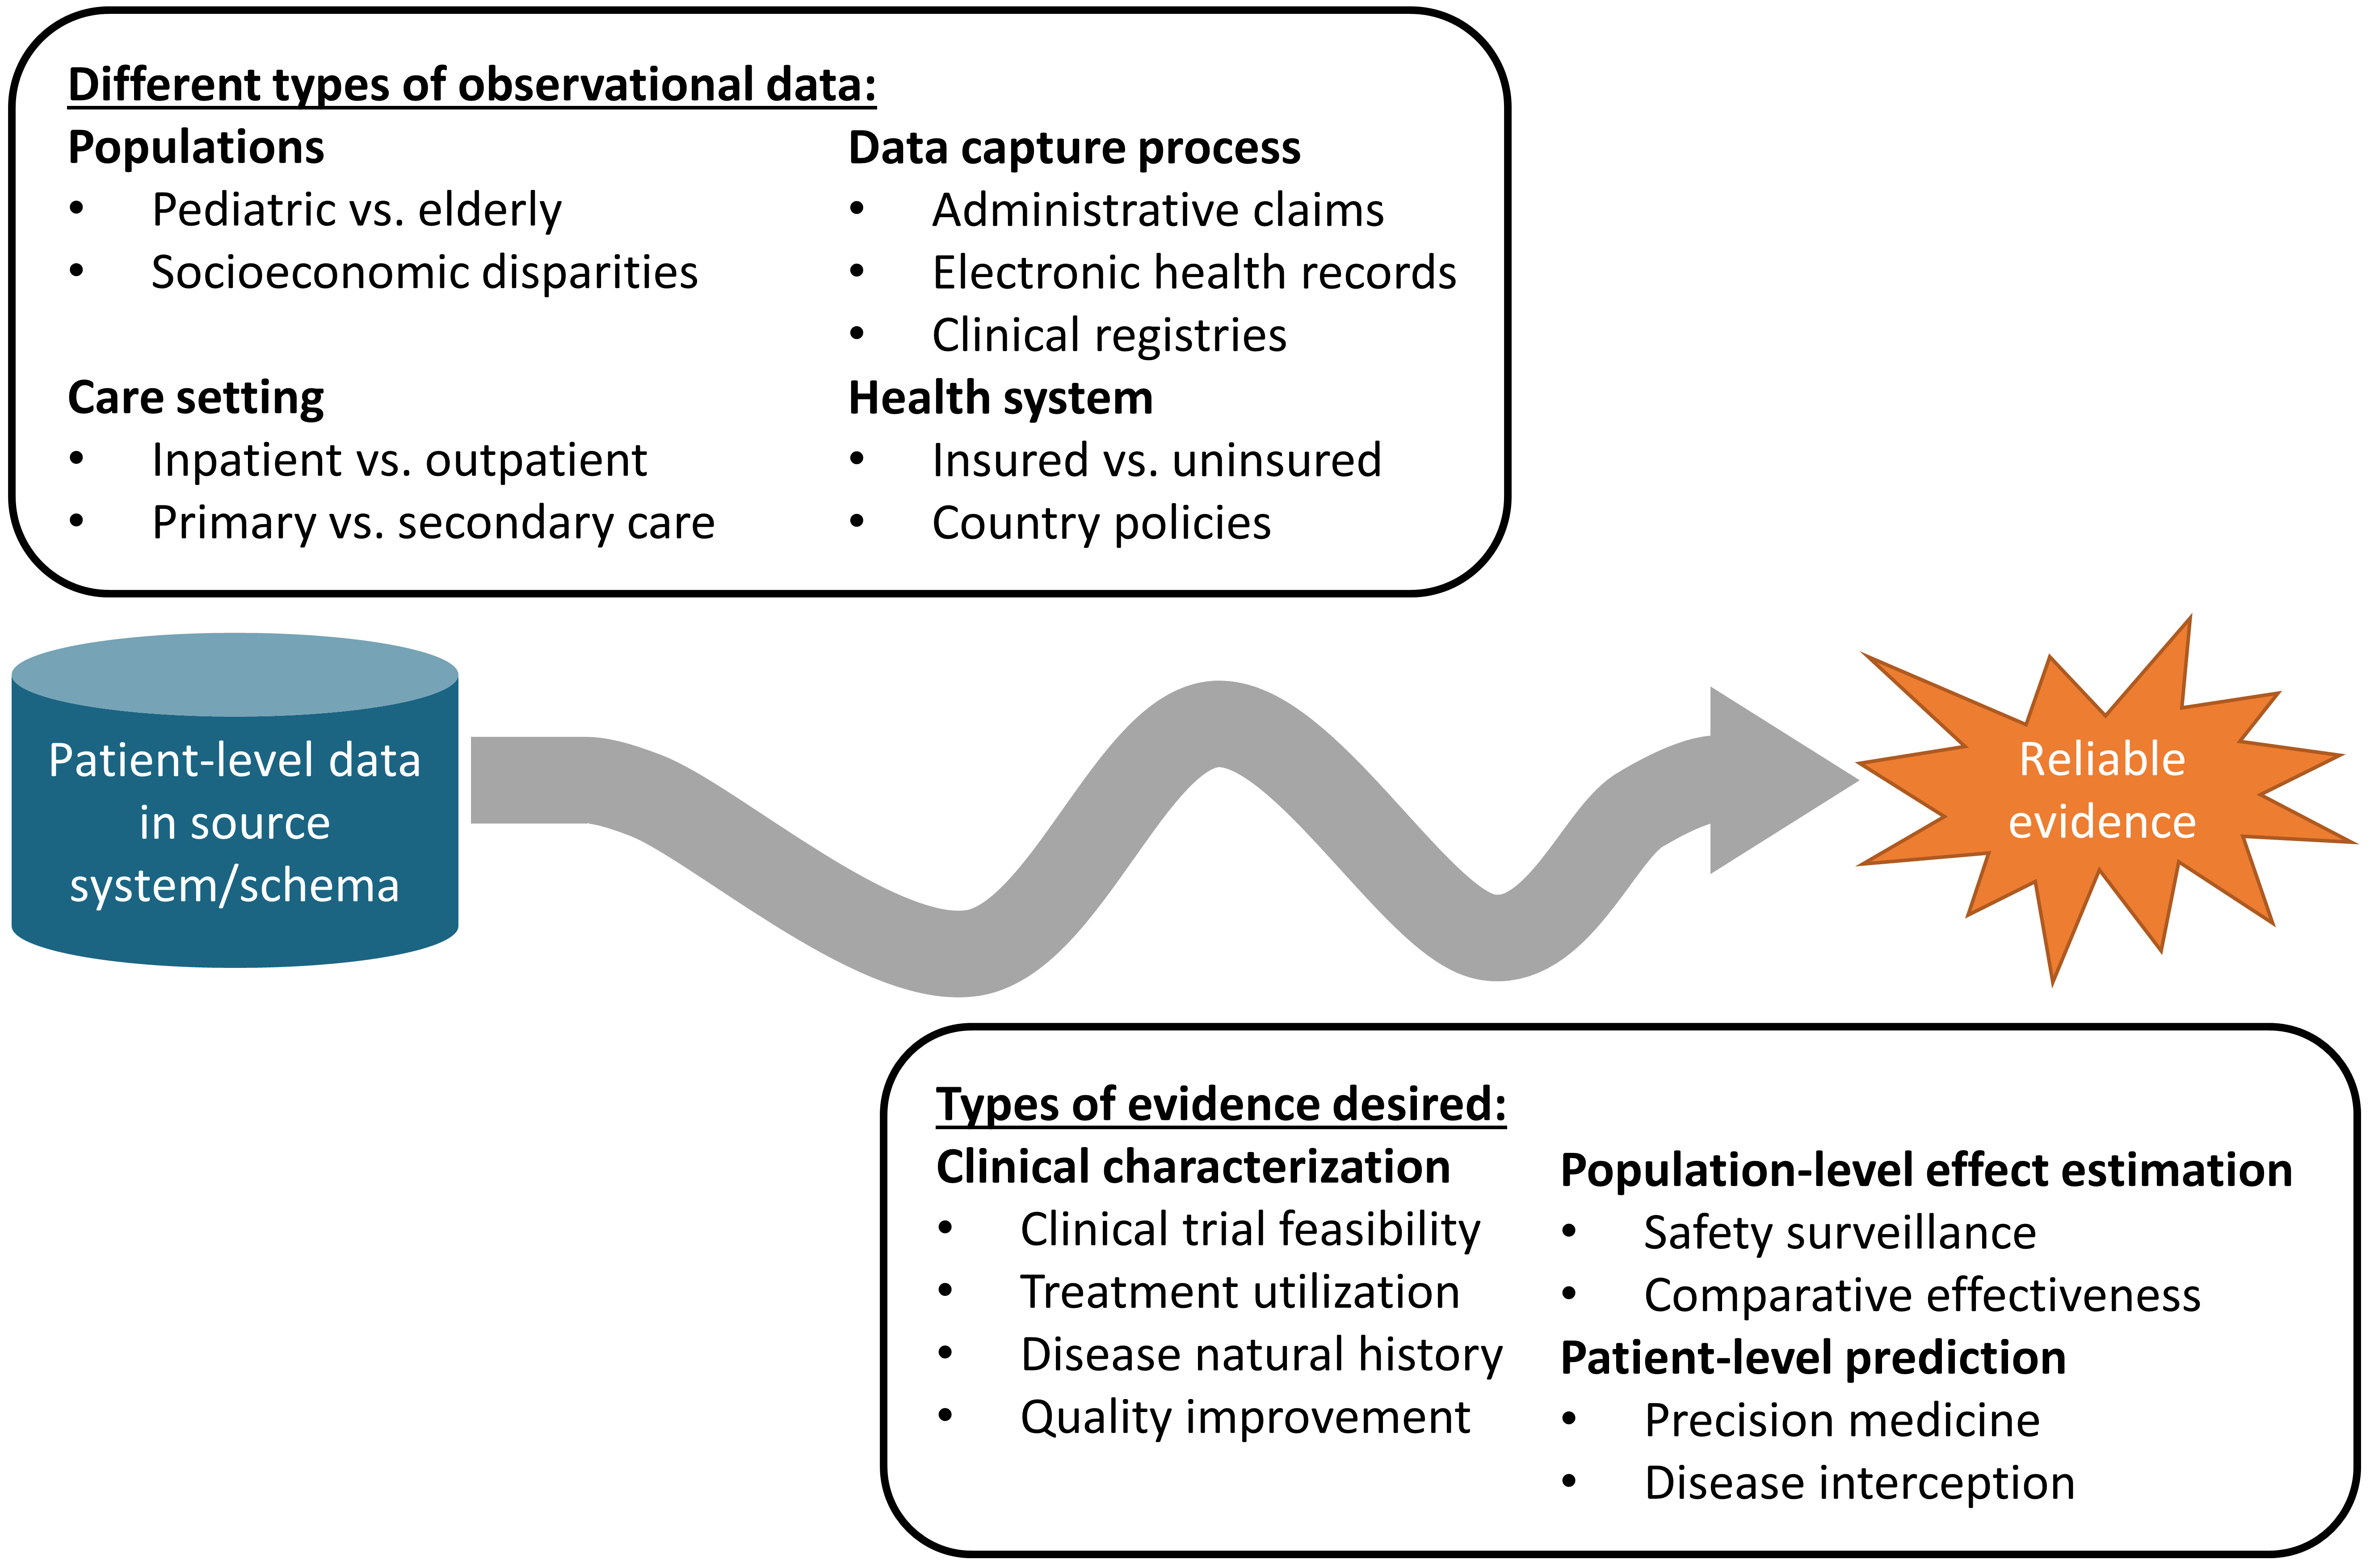
\includegraphics[width=1\linewidth]{images/OhdsiCommunity/datajourney} 

}

\caption{The journey from data to evidence}\label{fig:datajourney}
\end{figure}

원본 시스템에서 다양한 환자 수준의 데이터를 수집하는 여러 유형의 관찰
데이터베이스 (observational database)가 있다. 이 데이터베이스는 서로
다른 의료 시스템 내부의 인구, 치료 설정 및 데이터 수집 프로세스의
이질성만큼 다양하다. 의사 결정에 도움이 될 수있는 다양한 유형의 근거가
있으며, 환자 특성 분석 (clinical characterization), 인구 수준 추정
(population-level estimation) 및 환자 수준 예측 (patient-level
prediction) 으로 분류할 수 있다. 모집단 수준 영향 추정 및 환자 수준
예측의 분석 사용 사례로 분류 할 수 있습니다. 출발지 (원본 데이터) 및
원하는 목적지 (근거)와는 별도로, 여정을 수행하는 데 필요한 광범위한
임상, 과학 및 기술 역량들은 문제를 더욱 복잡하게 만든다. 보험 청구나
진료 과정이 데이터로 수집되면서 보건 정책이나 보험 환급과 관련된 행동
동기들로 인해 데이터 수집 및 정제 과정에서 발생할 수 있는 편향을
비롯하여, 환자와 의료 제공자간의 접점으로부터 원본 데이터가 발생하는
전반적인 과정에 대한 철저한 이해도 필요하다. 임상적 의문을 관련 해답을
도출하는 데 적합한 관찰 연구 설계으로 변환하기 위해선 역학 원칙과 통계적
방법을 숙지해야 한다. 수백만 명의 환자의 수년간의 종적 추적에 걸친
수십억 건의 임상 관찰을 가진 데이터셋에 대해 계산적으로 효율적인 데이터
과학 알고리즘을 구현하고 실행할 수 있는 기술적 능력 역시 필요하다.
관찰형 연구 통해 습득한 내용을 다른 종류의 근거와 통합하고, 이 새로운
지식이 건강 정책 및 임상 관행에 어떤 영향을 미칠지 결정하기 위해 임상
지식 또한 필요하다. 따라서, 한 개인이 데이터에서 근거를 성공적으로
만들어 내는 데 필요한 기술과 자원을 모두 보유하는 것은 매우 드문 일이다.
그보다는 이용 가능한 최선의 데이터를 가장 적절한 방법으로 분석하여 모든
이해당사자들이 의사결정 과정에 신뢰하고 사용할 수 있는 근거를 생산하는,
데이터에서 근거까지의 이 여정을 위해서는 보통 여러 개인과 조직의 협력이
필요하다.

\section{오몹 (Observational Medical Outcomes Partnership,
OMOP)}\label{-observational-medical-outcomes-partnership-omop}

협력 관찰형 연구 모델로써 주목할만한 예시로 오몹 (Observational Medical
Outcomes Partnership, OMOP)이 있었다. 오몹은 미국의 식품의약국 (FDA)이
주관하고, 미국 국립 보건원 (National Institutes of Health) 관리하에 학술
연구자 및 보건 데이터 파트너와 협력하는 제약 회사의 컨소시엄로
구성되었으며, 관찰형 보건의료 데이터를 이용하여 능동적 의료 제품 안전성
감시의 발전을 꾀하는 민관 협력체였다. \citep{stang2010omop} OMOP은
다수의 이해관계자 간의 거버넌스 구조를 확립했고, 다수의 청구자료 및 전자
의무 기록 데이터베이스에 적용하여 진정한 약물 안전성 연관성과 거짓 양성
소견을 식별할 수 있는 대안적인 역학 설계 및 통계 방법의 성능을
경험적으로 검증하는 일련의 방법론적 실험을 설계하였다. 분산되어 있는
관찰형 데이터 베이스를 통해 연구릴 진행함에 있어 기술적인 난제를
인식하고, 연구진들은 데이터의 구조, 내용 및 용어를 표준화하여 하나의
통계 분석 코드가 모든 데이터 파트너에서 사용될 수 있도록, OMOP 공통
데이터 모델 (Common Data Model, CDM) 을 설계하였다.
\citep{overhage2012cdm} OMOP 실험은 공통 데이터 모델과 표준화된 어휘를
확립하는 것이 가능하다는 것을 증명했다. 이는 서로 다른 관리
설정으로부터, 다른 용어 체계를 통해 다른 데이터 유형을 수용하고 하여
기관 간 협업과 효율적인 분석을 용이하게 할 수 있는 방식으로 구현되었다.

OMOP는 처음부터 연구 설계, 데이터 표준, 분석 코드, 경험적 결과 등 모든
작업 제품을 공공에 배포하여 투명성을 증진하고, OMOP가 수행하고 있는
연구에 대한 신뢰도를 쌓을 뿐 아니라, 또한 다른 이들의 연구 목적을 위하여
발전할 수 있도록 개방형 과학 (open science) 정책을 채택하였다. OMOP의
원래 초점은 약물 안전성이었지만, OMOP-CDM은 의료 처치와 보건 시스템
정책의 비교 효과성을 포함한 확대된 분석 사용 사례를 지원하기 위해
지속적으로 발전했다.

비록 OMOP이 대규모의 경험적 실험을 완성하는 데 성공하였고,
\citep{ryan2012omop, ryan2013omop} 방법론적인 혁신을 만들고,
\citep{schuemie_2014} 관찰형 데이터를 이용하여 안정성에 관련되어
의사결정에 유용한 지식 생성을 위한 적절한 방법론을 제시하였지만,
\citep{madigan_2013, madigan2013design} 이제 OMOP의 유산은 OHDSI
커뮤니티의 형성에 동기를 부여한 자극과 개방형 과학 원칙을 조기에 채택한
것으로 더 기억될 수 있다.

OMOP 프로젝트가 FDA의 능동 감시에 도움을 줄 숭 있는 관찰론적 연구를
완료하고 종료된 이후, 사람들은 OMOP 여정의 끝이, 새로운 여정의 시작이
되어야 된다고 생각했다. OMOP의 방법론적 연구가 관찰 데이터에서 생성되는
근거의 품질을 명시적으로 개선할 수 있는 과학적 모범 사례에 대한 가시적
통찰력을 제공함에도 불구하고, 그러한 모범 사례의 채택은 느렸다. 몇 가지
장애물들을 있었는데, 1) 방법론적의 혁신 이전에 관찰형 데이터 품질에 대한
근본적인 우려 2) 방법론적 문제와 해결책에 대한 불충분한 개념적 이해 3)
개별 데이터 파트너의 로컬 환경 내에서 솔루션을 독립적으로 구현할 수
없다는 점 4) 이러한 접근방식이 그들의 관심 임상 문제에 적용 가능한지에
대한 불확실성 등이었다. 이러한 모든 장애물에 대한 하나의 공통된 실마리는
한 사람만이 스스로 변화를 만드는 데 필요한 모든 것을 가지고 있지는
않지만, 여러 사람이 협력하면 이러한 문제들을 극복할 수 있다는 것이었다.

\begin{itemize}
\tightlist
\item
  기초 데이터 품질에 대한 신뢰도를 높이며 구조, 콘텐츠 및 의미론의
  일관성을 촉진하여 표준화된 분석이 가능하도록 개방형 커뮤니티의 (open
  community) 데이터 구조, 어휘 및 추출 변환 적재
  (Extract-Transform-Load, ETL)의 표준 규약 구축을 위한 협업
\item
  약물 안전성 연구 외에도 clinical characterization, population-level
  effect estimation, patient-level prediction을 위한 보다 광범위한 모범
  사례 (best practice)을 확립하기 위한 협업. 방법론적 연구를 통해 입증된
  과학적 모범 사례 구현을 코드화하고 연구자들이 쉽게 채택할 수 있는 오픈
  소스 분석 소프트웨어 개발에 대한 협업.
\item
  데이터에서 근거로의 여정을 인도해줄, 주요한 보건 문제에 대한 공동체
  공통의 질문에 대한 임상적 적용에 대한 협업
\end{itemize}

이러한 통찰을 통해, 오딧세이 (OHDSI)가 태어났다.

\section{개방형 협업 공동체로서의 오딧세이 (OHDSI as an Open-Science
Collaborative)}\label{----ohdsi-as-an-open-science-collaborative}

OHDSI (Observational Health data Sciences and Informatics, 오딧세이) 는
보다 더 나은 의료 결정과 더 나은 보건 관리를 촉진할 수 있는 과학적
근거를 공동으로 생성하도록 함으로써 보건 수준을 향상시키는 것을 목표로
하는 개방형 과학 공동체다. \citep{Hripcsak2015} OHDSI는 관찰 건강
데이터의 적절한 사용에 대한 과학적 모범 사례를 확립하기 위한 방법론적
연구를 수행하고, 이러한 연구방법론을 일관되고 투명하며 재현 가능한
솔루션으로 코드화하는 오픈 소스 분석 소프트웨어를 개발하여, 보건의료
정책 및 환자 치료에 도움이 될 수 있는 임상적 근거를 마련하는 데에 적용할
수 있도록 노력한다.

\subsection{OHDSI의 사명 (Our Mission)}\label{ohdsi--our-mission}

참여 공동체의 상호협력 하에 의료 발전을 촉진하는 근거를 생성하는 능력을
부여한다.

\begin{quote}
To improve health by empowering a community to collaboratively generate
the evidence that promotes better health decisions and better care.
\index{mission}
\end{quote}

\subsection{OHDSI의 이상 (Our Vision)}\label{ohdsi--our-vision}

의료 빅데이터의 분석을 통해 세계에 건강과 질병에 대한 포괄적인 이해를
제공한다.

\begin{quote}
A world in which observational research produces a comprehensive
understanding of health and disease. \index{vision}
\end{quote}

\subsection{OHDSI의 핵심 가치 (Our
Objectives)}\label{ohdsi---our-objectives}

\begin{itemize}
\tightlist
\item
  \textbf{혁신성 Innovation}: 우리는 적극적으로 의료 빅데이터 분석 및
  연구에 대한 혁신적인 방법론과 접근법을 찾고 격려한다.
\end{itemize}

\begin{quote}
Observational research is a field which will benefit greatly from
disruptive thinking. We actively seek and encourage fresh methodological
approaches in our work.
\end{quote}

\begin{itemize}
\tightlist
\item
  \textbf{재현성 Reproducibility}: 우리는 보건 증진을 위하여 정확하고,
  재현 가능하며, 잘 보정된 근거를 찾도록 노력한다.
\end{itemize}

\begin{quote}
Accurate, reproducible, and well-calibrated evidence is necessary for
health improvement.
\end{quote}

\begin{itemize}
\tightlist
\item
  \textbf{공동체 정신 Community}: 우리는 모든 참여자들을 환영하며
  동등하게 우리의 활동에 참여할 수 있도록 돕는다.
\end{itemize}

\begin{quote}
Everyone is welcome to actively participate in OHDSI, whether you are a
patient, a health professional, a researcher, or someone who simply
believes in our cause.
\end{quote}

\begin{itemize}
\tightlist
\item
  \textbf{개방성 Openness}: 우리는 의사 결정 과정의 투명성을 지향하며,
  우리의 진보 및 우리가 생성한 방법론, 소프트웨어, 근거를 가능한
  공개적으로 접근 가능하게 한다.
\end{itemize}

\begin{quote}
We strive to make all our community's proceeds open and publicly
accessible, including the methods, tools and the evidence that we
generate.
\end{quote}

\begin{itemize}
\tightlist
\item
  \textbf{협력 정신 Collaboration}: 우리는 참여자들의 실제적 요구를
  우선적으로 다루고, 그것을 위해 공동으로 노력한다.
\end{itemize}

\begin{quote}
We work collectively to prioritize and address the real world needs of
our community's participants.
\end{quote}

\begin{itemize}
\tightlist
\item
  \textbf{선행의 정신 Beneficence}: 우리는 고통 받는 환자를 비롯하여
  참여자 및 참여기관의 권리를 보호하기 위해 노력한다.
\end{itemize}

\begin{quote}
We seek to protect the rights of individuals and organizations within
our community at all times.
\end{quote}

\index{objectives}

\section{오딧세이의 진척 (OHDSI's Progress)}\label{--ohdsis-progress}

OHDSI는 2014년 설립된 이래 성장을 지속하여 컴퓨터 과학, 역학, 통계, 생물
의학 정보학, 보건 정책 및 임상 의학 등 다양한 분야를 대표하는 학계, 의료
제품 산업, 규제 기관, 정부, 보험자, 기술 제공자, 의료 시스템, 임상의사
및 환자 집단 2,500명 이상의 다양한 이해관계자이 온라인 포럼에서 활동하고
있다. OHDSI 협력체로써 자발적으로 보고한 기관 및 데이터베이스의 리스트는
OHDSI 웹사이트에서 확인할 수 있다. \footnote{\url{https://www.ohdsi.org/who-we-are/collaborators/}}
오딧세이 협력 지도 (Figure \ref{fig:collaboratormap}) 는 폭넓은 국제
공동체로써의 다양성을 상기시킨다.

\begin{figure}

{\centering 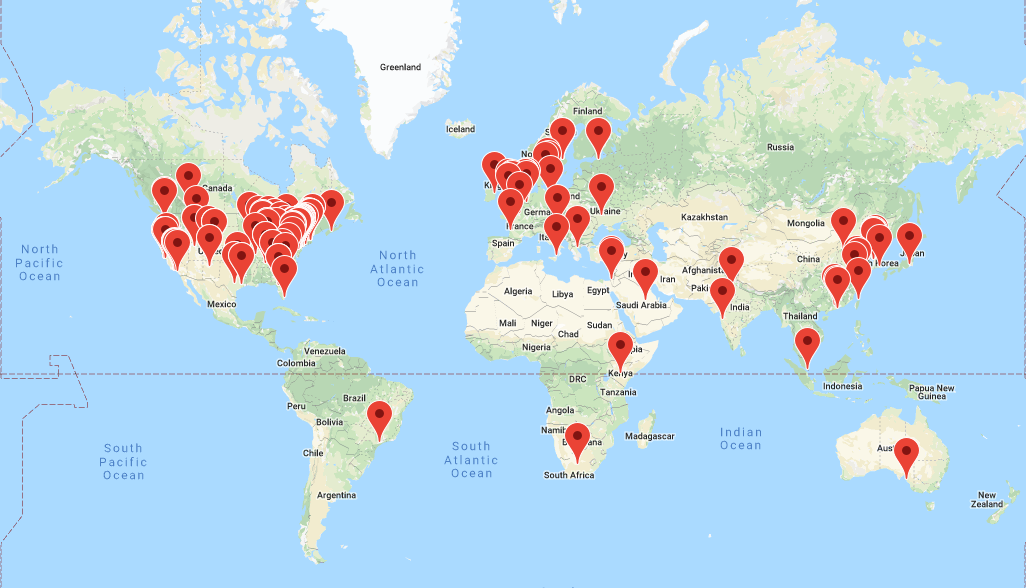
\includegraphics[width=1\linewidth]{images/OhdsiCommunity/mapOfCollaborators} 

}

\caption{Map of OHDSI collaborators as of August, 2019}\label{fig:collaboratormap}
\end{figure}

OHDSI는 OMOP-CDM이라는 개방형 공동체 데이터 표준 기반으로 2019년 8월
기준으로 20여개국, 100개 이상의 의료 데이터베이스들로 구성된 분산형
연구망 (distributed research network, DRN)을 구축했다. 분산형 연구망이란
환자 수준의 데이터를 개인이나 조직 간에 공유할 필요가 없다는 것을
의미한다. 분산연구망에서는, 데이터를 기관 폐쇄망 안에 두고 연구자는
프로토콜 형태의 분석코드/프로그램을 공유한다. 데이터 파트너들은 연구자의
요청에 따라 기관 안에서 연구 프로토콜을 실행해 자동으로 생성되는 요약
집합정보(평균, 합, 표준편차, 오즈비, 위험도 등)만 연구자에게 회신하는
방식으로, 연구자는 폐쇄망 안에 있는 환자의 개별 정보를 보거나 취득하지
않는다. OHDSI 분산망에서 각 데이터 파트너는 환자 수준 데이터의 사용에
대한 완전한 자율성을 유지하고, 각 기관의 데이터 거버넌스 정책을
지속적으로 준수한다.

OHDSI 개발자 커뮤니티는 3가지의 사용 사례를 지원하기 위해 OMOP CDM 위에
다음 3가지의 강력한 오픈 소스 분석 소프트웨어 라이브러리를 구축하였다.

\begin{enumerate}
\def\labelenumi{\arabic{enumi})}
\tightlist
\item
  Clinical characterization: 질병의 자연 경과, 치료 행태 및 질 향상을
  위한 임상 특성 분석
\item
  Population-level effect estimation: 의약품 안전성 감시 및 비교 효과
  연구에서의 인과성 분석
\item
  Patient-level prediction: 머신러닝 알고리즘을 활용한 정밀 의학 또는
  의료 개입
\end{enumerate}

OHDSI 개발자들은 또한 OMOP CDM의 채택, 데이터 품질 평가, OHDSI 네트워크
연구의 촉진을 지원하는 애플리케이션을 개발했다. 이러한 소프트웨어에는
R과 Python에 내장된 백엔드 통계 패키지 및 HTML과 Javascript로 개발된
프론트엔드 웹 어플리케이션이 포함된다. 모든 OHDSI 소프트웨어들은 오픈
소스 정책을 채택하여 Github을 통해 공개된다. \footnote{\url{https://github.com/OHDSI}}

오픈 소스 소프트웨어들과 함께, OHDSI의 개방형 과학 공동체적 접근은
관찰형 연구의 발전을 가능하게 했다. 첫번째 OHDSI 네트워크 연구는 당뇨,
우울증, 고혈압의 3가지 만성 질병에 대한 치료 패턴을 분석하는 것이었다.
PNAS(Proceedings of the National Academy of Science) 에 출판된 연구는,
그 때까지 수행된 최대 규모의 관찰형 연구로써 11개의 데이터베이스에서 2억
5천만명의 환자 데이터를 이용하여 이전에 보고된 적 없는 치료 패턴의
지역적 차이 및 환자별 치료선택에 대한 이질성에 대해 발표하였다.
\citep{Hripcsak7329} OHDSI는 교란변수를 통제하는 새로운 통계적 방법론을
제시하였고, \citep{tian_2018} 인과성 검증 능력에 대해 검증하였고,
\citep{schuemie_2018} 이러한 방법론을 뇌전증 약제의 개별 안전성 연구
\citep{duke_2017} 및 당뇨병의 이차 약제의 비교 효과 연구
\citep{vashisht_2018} 및 우울증 치료의 대규모 비교 효과 연구
\citep{schuemie_2018b}에 활용하였다. OHDSI 공동체는 또한 관찰형 보건의료
데이터의 머신러닝 알고리즘을 활용 프레임 워크를 구축 \citep{reps2018}
하여 다양한 치료 분야에 활용하였다.
\citep{johnston_2019, cepeda_2018, reps_2019}

\section{Collaborating in OHDSI}\label{collaborating-in-ohdsi}

OHDSI는 근거를 생성하기 위해 협업을 강화하는 것을 목표로 하는
공동체인데, OHDSI 참가자가 된다는 것은 무엇을 의미하는가? 만약 당신이
OHDSI의 사명을 믿고 데이터에서 근거에 이르는 여정의 어디든지 기여를 하는
데 관심이 있다면, OHDSI는 당신을 위한 공동체가 될 수 있다. OHDSI
참가자는 보건 의료 데이터에 접근이 가능하고, 이를 활용해 의학적 근거를
생성하고 싶은 개인일 수 있다. OHDSI 참가자는 과학적 모범 사례를 수립하고
대안적 접근법을 평가하는 데 관심이 있는 방법론 연구자일 수 있다. OHDSI
참가자는 OHDSI의 타 연구자들이 사용할 수 있는 도구를 만들기 위해
프로그래밍 기술을 적용하는 데 관심이 있는 소프트웨어 개발자일 수 있다.
OHDSI 참가자는 중요한 의학보건학적 질문을 가지고 있고 논문 발표 등을
통해 그러한 질문들에 대한 근거를 보다 더 큰 의료 커뮤니티에 제공하고자
하는 임상 연구자일 수 있다. OHDSI 참가자는 공공 보건을 위해 이러한
공통적인 사명과 가치를 믿고 해당 지역의 공동체가 OHDSI 관련 교육과
심포지엄 개최를 포함하여, 그 임무를 지속할 수 있도록 자원을 제공하는
개인 또는 단체일 수도 있다. 당신의 배경이나 소속과 관계없이, OHDSI는
개개인이 공통의 목적을 위해 함께 일할 수 있는 공동체가 되기를 추구하고
있으며, 각 개인이 공동으로 의료 서비스를 발전시킬 수 있는 기여를 하고
있다. 이 여정에 함께하고 싶다면, 챕터 \ref{WhereToBegin} (``Where To
Begin'') 를 통해 어떻게 시작하는 지 배울 수 있다.

\section{한국 오딧세이의 역사}\label{--}

아주대학교 박래웅 교수가 아주대 병원의 전자의무기록을 이용하여 2014년
OMOP-CDM 도입을 시작하였고, 2015년 첫 연례 심포지엄에서 활용 결과를
발표하면서 한국의 OHDSI 참여가 시작되었다. 이후 계속적으로 한국에서
OMOP-CDM, OHDSI 전파를 위해 노력하였고, 2016년부터는 최초로 국제 OHDSI
committee에서 개별 국가를 위한 포럼
\href{http://forums.ohdsi.org/c/For-collaborators-wishing-to-communicate-in-Korean}{Korean
chapter}을 개설하고, 한국의 OHDSI 참여를 독려하였다. 첫 한국 국제
오딧세이 심포지엄은 2017년 3월 아주대학교에서 튜토리얼, 리더십 미팅을
포함하여 3일간 개최되었다.

\begin{figure}
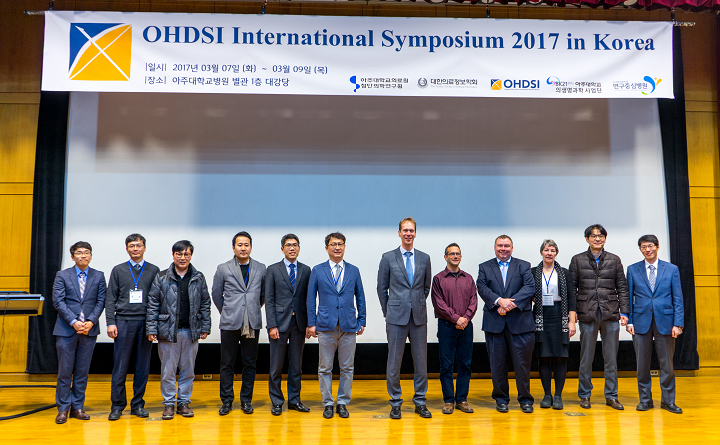
\includegraphics[width=0.8\linewidth]{images/OhdsiCommunity/DSC01956} \caption{OHDSI International Symposium 2017 in Korea}\label{fig:OHDSIInternationalSymposium2017inKorea1}
\end{figure}\begin{figure}
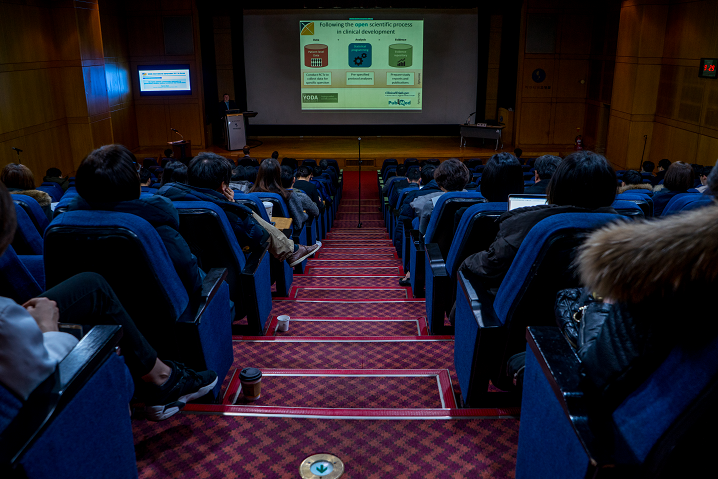
\includegraphics[width=0.8\linewidth]{images/OhdsiCommunity/DSC01861} \caption{OHDSI International Symposium 2017 in Korea}\label{fig:OHDSIInternationalSymposium2017inKorea1}
\end{figure}

\begin{figure}
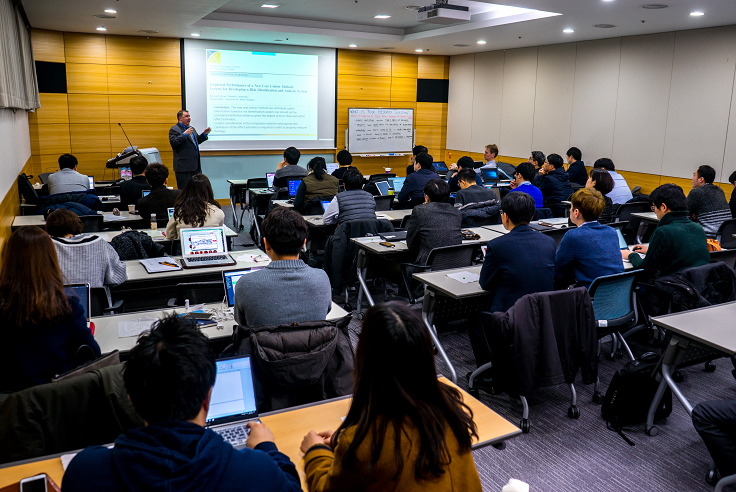
\includegraphics[width=0.8\linewidth]{images/OhdsiCommunity/DSC02166} \caption{Tutorial in the OHDSI International Symposium 2017}\label{fig:OHDSIInternationalSymposium2017inKorea2}
\end{figure}

한국 OHDSI 네트워크에 참여를 희망하는 병원 관계자들과 함께 2017년 3월
7일 첫번째 리더십 미팅을 가진 후 현재까지 2달마다 전국의 의과대학/병원을
순회하며 한국 OHDSI 리더십 미팅을 개최하며 OHDSI 전파 및 상호 협력을
꾀하고 있다.

\section{Summary}\label{summary}

\BeginKnitrBlock{rmdsummary}
\begin{itemize}
\item
  OHDSI의 사명은 참여 공동체의 상호협력 하에 의료 발전을 촉진하는 근거를
  생성하는 능력을 부여하는 것이다.
\item
  OHDSI의 이상은 혁신성, 재현성, 공동체 정신, 개방성, 협력 정신, 선행의
  정신을 바탕으로 의료 빅데이터의 분석을 통해 세계에 건강과 질병에 대한
  포괄적인 이해를 제공하는 것이다.
\item
  OHDSI 참가자들은 개방형 공동체로서의 데이터 표준, 방법론 연구,
  오픈소스 분석 소프트웨어 개발 및 임상적 적용을 통해 데이터로부터
  근거로의 여정을 발전시키고자 노력한다.
\end{itemize}
\EndKnitrBlock{rmdsummary}

\chapter{어디서부터 시작할 것 인가 (Where to Begin)}\label{WhereToBegin}

\emph{Chapter leads: Hamed Abedtash \& Kristin Kostka}

\begin{quote}
``천리길도 한 걸음부터'' - 노자
\end{quote}

OHDSI 커뮤니티는 학계, 산업 및 정부기관 전반에 걸쳐 다양한
이해관계자들을 대표하고 있다. 본 커뮤니티의 작업으로 의료 시스템 뿐
아니라 환자, 의료제공자, 연구자들을 포함한 다양한 개인들과 기관들이
혜택을 받게 된다. 이러한 이점은 이해관계자들에게 의료 데이터 를 더
유용하게 해주고 의료데이터 분석의 질도 향상시켜주는 덕분이다. 관찰연구는
파괴적인 생각(disruptive thinking)으로부터 혜택을 받는 분야라고
생각한다. 우리는 새로운 방법론적인 접근법을 적극적으로 추구하고
장려합니다. \index{community}

\section{여정에 동참 하십시오}\label{--}

환자, 의료 전문가, 연구원 혹은 단순히 OHDSI의 목적에 동감하는 사람이든
누구든지 OHDSI 커뮤니티에 적극적으로 참여할 수 있다. OHDSI는 포용적
멤버십 모델을 추구하며 OHDSI의 공동연구자가 되기 위한 멤버십 비용은
없다. 참여를 원하는 사람은 단지 손을 들어서 매년 OHDSI 멤버십 카운트에
포함되면 된다. 참여는 전적으로 자의에 의한 것이며 매주 커뮤니티의
네트워크 스터디나 OHDSI 작업 그룹에 참여하는 것 만으로도 충분하다. 꼭
데이터를 보유하고 있어야만 OHDSI 커뮤니티의 액티브 멤버가 되는 것은
아니며 본 커뮤니티는 데이터 보유자, 연구원, 헬스케어 제공자, 환자와
소비자 모두에게 도움을 주고자 한다. 공동연구자의 프로필은 OHDSI
웹사이트에서 관리되고 정기적으로 업데이트 되고 있다. 멤버십은 OHDSI
커뮤니티 콜, 워크그룹, 지역별 모임을 통해 육성되고 있다.
\index{join the journey} \index{workgroups} \index{chapters}

\begin{figure}

{\centering 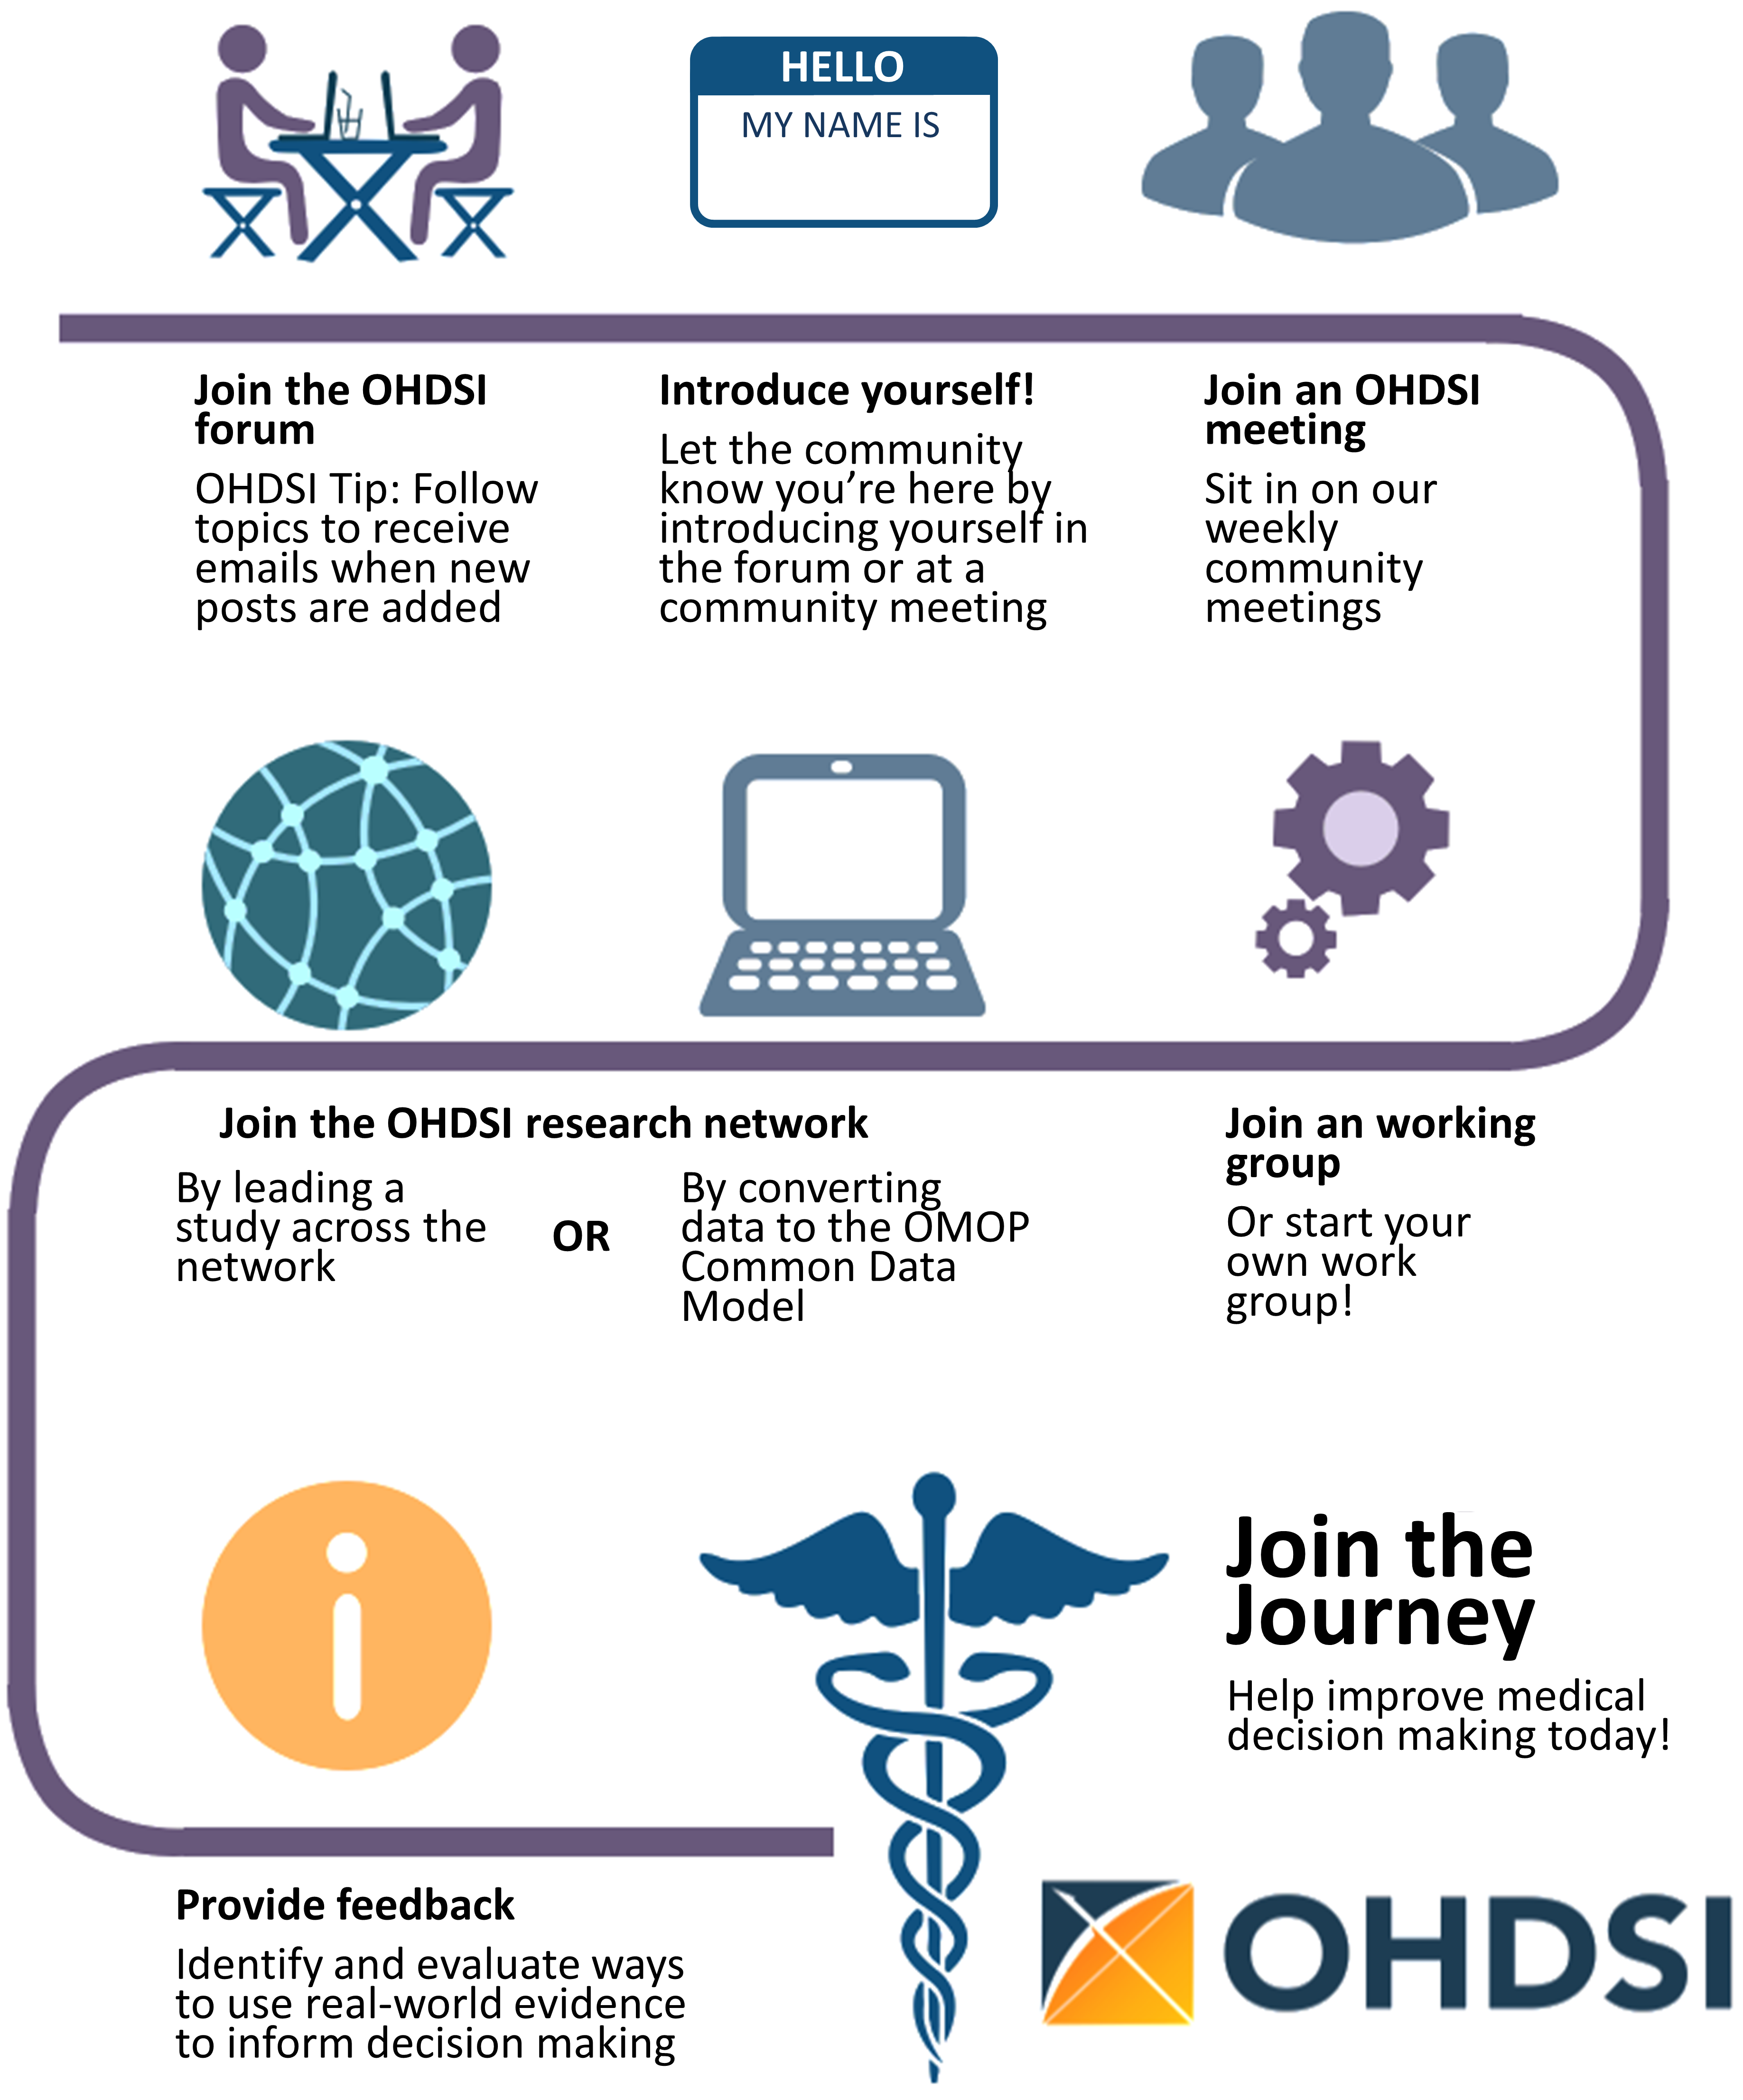
\includegraphics[width=0.9\linewidth]{images/WhereToBegin/joinTheJourney} 

}

\caption{특성 분석 결과 - 하나의 concept에 대하여 자세한 내용이 들어있는 새로운 창.}\label{fig:jointhejourney}
\end{figure}

\hypertarget{ohdsi-}{\subsection{OHDSI 포럼}\label{ohdsi-}}

OHDSI 포럼1은 OHDSI 커뮤니티 공동연구자들이 메시지를 올리는 형식을 통해
대화하는 온라인 토론 사이트이다. 포럼은 트리와 같은 구조로 구성되었다.
가장 상위에는 ``카테고리''가 있으며 관련성 있는 토론 카테고리로
나눠진다. 각 카테고리 아래로는 하위 포럼과 추가적인 하위 포럼들로
구성된다. 각 토픽(스레드라고도 불림)의 가장 낮은 하위 포럼에서 포럼
멤버들간의 토론 혹은 포스트가 작성된다.

OHDSI 포럼에서는 다음을 포함한 콘텐츠 카테고리를 찾을 수 있다:

\begin{itemize}
\tightlist
\item
  \textbf{일반}: OHDSI 커뮤니티와 참여 방법에 대한 전반적인 토론
\item
  \textbf{시행자}: 로컬 환경에서 공동 데이터 모델과 OHDSI 분석
  프레임워크 구현하는 방법에 대한 토론
\item
  \textbf{개발자}: OHDSI 어플리케이션의 오픈 소스 개발과 OMOP CDM과의
  균형을 위한 도구에 관한 논의
\item
  \textbf{연구원}: OHDI 연구 네트워크를 위한 근거 발생, 공동 연구,
  통계적 방법과 기타 CDM 기반 연구의 다른 토픽들에 관한 토론
\item
  \textbf{CDM 개발자}: 진행중인 CDM을 위한 조건, vocabulary 그리고
  테크닉적인 요소들에 관한 토론
\item
  \textbf{Vocabulary 유저}: Vocabulary 콘텐츠에 관한 토론
\item
  \textbf{지역 지부(예: 한국, 중국, 유럽)}: 지역별 언어로 진행되는 로컬
  OMOP 구현과 OHDSI 커뮤니티 활동에 관한 토론
\end{itemize}

개별적인 주제로 포스팅을 올리려면 계정 등록을 먼저 해야 한다. 포럼
계정을 오픈하고 나면 General Topic 아래 ``Welcome to OHDSI! -- Please
introduce yourself''라는 토픽에 본인 소개를 하는 것을 추천한다.\\
1) 본인 소개 및 본인의 업무 소개 2) 커뮤니티 안에서 어떤 방식으로 도움을
줄 수 있는지 (예: 소프트웨어 개발, 연구, 연구 논문 작성 등)를 본인
소개에 설명한다. 이제 OHDSI 여정에 동참하였습니다! 이 후엔 토론에
참여하는 것을 권장합니다. OHDSI 커뮤니티 포럼을 통해 자신의 질문을
포스팅하고 새로운 아이디어와 협업에 참여하시기 바랍니다. \index{forum}

\BeginKnitrBlock{rmdimportant}
토픽을 ``watch'' 할 수도 있다. 이 뜻은 관심있는 토픽에 새로운 포스트가
올라올 경우, 이메일로 안내를 받고 이메일 답장을 통해 다시 답장을 보낼
수도 있다. 앞으로 다가올 미팅에 대한 아젠다도 확인할 수 있으며
공동작업기회와 주간 OHDSI 다이제스트를 개별 이메일 받은편지함에서 수령할
수 있다.
\EndKnitrBlock{rmdimportant}

\hypertarget{ohdsi-}{\subsection{OHDSI 이벤트}\label{ohdsi-}}

OHDSI는 정기적으로 직접 참여가 가능한 이벤트를 개최하여 공동연구자들이
서로 학습하고 향후 협력 관계를 강화할 수 있는 기회를 제공한다. 이러한
이벤트는 OHDSI웹사이트를 통해 전달되며 참석에 관심이 있는 사람들에게
무료로 제공된다.

OHDSI 심포지엄은 미국, 유럽, 아시아 등에서 매년 개최되는 과학
컨퍼런스로, 이를 통해 공동 연구자들이 총회, 포스터 발표 및 소프트웨어
시연 등을 통해 각각의 최신 연구를 발표할 수 있다. OHDSI심포지엄은
커뮤니티 내에서 최신의 진행상황을 배울 수 있는 네트워크를 위한 훌륭한
장소를 제공하고 있다. 일반적으로 OHDSI심포지엄은 새로운 커뮤니티
참여자들이 데이터 표준과 분석에 대한 모범사례에 관한 주제들에 대해
실질적 참여 기회를 가질 수 있도록 동료 공동연구자들이 강의 교수로 참여는
OHDSI 튜토리얼이 함께 진행된다.

OHDSI공동연구자들의 대면 이벤트는 좀더 규모가 작은 포럼인데, 일반적으로
함께 관심을 가지게 될 문제들에 중심으로 구성된다. 지난 이벤트들 중에는
``Phenotype hack-a-thon'', ``데이터 퀄리티 hack-a-thon'', ``오픈소스
소프트웨어 documentation-a-thon'' 등이 있었다. OHDSI는 다양한
study-a-thon 이벤트를 개최했으며 이를 통해 공동연구자들이 며칠간 함께
팀이 되어 특정 연구 질문에 대하여 적절한 관찰 분석과 OHDSI 네트워크에
관한 학습, 대중 보급을 위한 근거 합성을 할 수 있는 기회를 제공하였다.
이런 행사들에서, 공통의 문제를 해결하려는 공동의 희망과 관심사가
보였는데, 배움과 지속적인 발전을 도모하는 환경을 제공하였다.

OHDSI 커뮤니티의 힘을 보다 자세히 배우기 바란다. OHDSI 웹사이트의
\href{https://www.ohdsi.org/past-events/}{OHDSI Past Events section}에서
지난 심포지엄, 대면 미팅, OHDSI 튜토리얼 등을 접할 수 있다.

\subsection{OHDSI 커뮤니티 콜}\label{ohdsi--}

OHDSI 커뮤니티 콜은 매주 OHDSI 커뮤니티 안에서 발생하는 활동들에 대해
배울 수 있는 기회이다. 매주 화요일 오후 12시부터 1시 (동부시각)에 전화
컨퍼런스로 진행되고 있으며 OHDSI 커뮤니티가 최근 개발된 사항을 공유하고
개별 공동 연구자들 및 그룹 활동과 커뮤니티의 전체적인 성과를 알 수 있는
기회이다. 주간 미팅은 모두 녹음되고 있으며 발표자료들은 OHDSI 웹사이트
리소스에 기록된다.

모든 OHDSI공동 연구자들은 주간 전화 컨퍼런스에 초청되고 커뮤니티 토론을
위한 주제를 제안하도록 권유된다. OHDSI 커뮤니티 콜은 연구 결과를
공유하고 현재 활발히 진행중인 작업에 대한 의견을 제시하고 피드백을
얻으며, 개발 중인 오픈소스 소프트웨어를 시연하고, 데이터 모델링과 분석에
대한 모범사례를 커뮤니티와 함께 논의하고, 보조금/간행/컨퍼런스 워크샵
등을 위한 미래의 공동 작업 기회에 대해 많은 아이디어를 논의하는 포럼이
될 수 있다. 만약 당신이 다가올 OHDSI 공동연구자 미팅의 주제에
공동연구자라면, OHDSI 포럼에 초청받아서 본인 의견을 올릴 수 있다.

OHDSI 커뮤니티에 새로 들어온 사람은 이런 콜 시리즈를 개별 일정에
추가하여 OHDSI 네트워크 내에서 일어나는 일들에 대하여 숙지하는 것이
좋다. OHDSI 콜에 참여하기 원한다면
\href{https://www.ohdsi.org/web/wiki/doku.php?id=projects:ohdsi_community}{OHDSI
Wiki}를 참고하기 바란다. 커뮤니티 콜의 주제는 매주 다르다. OHDSI 포럼의
OHDSI 주간 다이제스트를 통해 매주 발표주제에 관한 정보를 받을 수 있다.
새로 온 사람은 처음 참여하는 콜에서 초청받으면 본인의 백그라운드와 OHDSI
가입 동기에 관해 소개한다. \index{community!community calls}

\hypertarget{ohdsi-}{\subsection{OHDSI 워크그룹}\label{ohdsi-}}

OHDSI 는 워크그룹 팀들이 이끌어가는 다양한 프로젝트들이 있다. 각각의
워크그룹은 커뮤니티에 기여하기 위한 프로젝트의 objective, goal,
artifacts 등을 결정하는 리더십 팀을 가지고 있다. 워크그룹 참여는
프로젝트 objective와 goal에 기여하고 싶은 참가자들에게 열려있다.
워크그룹은 오래된 전략적 목표를 가지고 있거나 커뮤니티의 특정 필요를
충족시키기 위한 단기 프로젝트일 수도 있다. 워크그룹의 정기 미팅은
프로젝트 리더들에 의해 결정되며 그룹마다 각각 다르다. 활동중인
워크그룹들의 리스트는
\href{https://www.ohdsi.org/web/wiki/doku.php?id=projects:overview}{OHDSI
Wiki}에서 관리되고 있다. \index{workgroups}

테이블 \ref{tab:OHDSIworkgroups}은 활동중인 OHDSI워크그룹의 빠른
레퍼런스를 제공한다. 프로젝트에 참여하여 배우길 독려한다.

테이블: \label{tab:OHDSIworkgroups}주목할 만한 OHDSI 워크그룹

\begin{longtable}[]{@{}lll@{}}
\toprule
\begin{minipage}[b]{0.19\columnwidth}\raggedright\strut
Workgroup Name\strut
\end{minipage} & \begin{minipage}[b]{0.16\columnwidth}\raggedright\strut
Objective\strut
\end{minipage} & \begin{minipage}[b]{0.22\columnwidth}\raggedright\strut
Target Audience\strut
\end{minipage}\tabularnewline
\midrule
\endhead
\begin{minipage}[t]{0.19\columnwidth}\raggedright\strut
Atlas \& WebAPI\strut
\end{minipage} & \begin{minipage}[t]{0.16\columnwidth}\raggedright\strut
Atlas \& WebAPI는 OHDSI 오픈소스 소프트웨어 구성의 일환으로 OMOP 공통
데이터 모델을 기반으로 한 표준화된 분석 기능을 제공하는 것에 중점을 두고
있다.\strut
\end{minipage} & \begin{minipage}[t]{0.22\columnwidth}\raggedright\strut
오픈소스 Atlas/WebAPI 플랫폼의 개선과 기여하고 싶은 Java와 JavaScript
소프트웨어 개발자들\strut
\end{minipage}\tabularnewline
\begin{minipage}[t]{0.19\columnwidth}\raggedright\strut
CDM \& Vocabulary\strut
\end{minipage} & \begin{minipage}[t]{0.16\columnwidth}\raggedright\strut
체계적이고 표준화되었으며 임상 환자 데이터에 적용되는 대량 분석을 위한
OMOP 공통 데이터 모델의 지속적인 개발. 타 워크그룹에 의해 개발된
표준화된 분석을 지원하기 위해 국제 코딩 시스템과 환자 케어의 임상적
측면의 증가를 통해 표준화된 Vocabulary의 질적 개선.\strut
\end{minipage} & \begin{minipage}[t]{0.22\columnwidth}\raggedright\strut
모든 필요와 사례들에 적용될OMOP 공통 데이터 모델과 표준화된 Vocabulary를
개선하고 싶은 사람\strut
\end{minipage}\tabularnewline
\begin{minipage}[t]{0.19\columnwidth}\raggedright\strut
Genomics\strut
\end{minipage} & \begin{minipage}[t]{0.16\columnwidth}\raggedright\strut
환자들의 게놈 데이터의OMOP 공통 데이터 모델로의 포함을 위한 확장. 다양한
시퀀싱 작업을 통해 유전 변종을 저장하고 있는 CDM-compatible schema의
정의를 내리는 그룹\strut
\end{minipage} & \begin{minipage}[t]{0.22\columnwidth}\raggedright\strut
제한 없음\strut
\end{minipage}\tabularnewline
\begin{minipage}[t]{0.19\columnwidth}\raggedright\strut
Population- Level Estimation\strut
\end{minipage} & \begin{minipage}[t]{0.16\columnwidth}\raggedright\strut
정확하고 믿을 수 있으며 재현가능한 population level estimates of
effects를 얻기 위한 관찰 연구의 과학적 방법을 개발하여 커뮤니티에 이러한
방법의 사용을 촉진한다.\strut
\end{minipage} & \begin{minipage}[t]{0.22\columnwidth}\raggedright\strut
제한 없음\strut
\end{minipage}\tabularnewline
\begin{minipage}[t]{0.19\columnwidth}\raggedright\strut
Natural Language Processing\strut
\end{minipage} & \begin{minipage}[t]{0.16\columnwidth}\raggedright\strut
OHDSI umbrella 아래의 관찰 연구를 위한 전자 의무기록의 텍스트 정보
사용의 홍보. 이 목표를 촉진하기 위해 이 그룹은OHDSI 커뮤니티의 연구 임상
텍스트의 활용을 구현할 수 있는 소프트웨어와 방법을 개발한다.\strut
\end{minipage} & \begin{minipage}[t]{0.22\columnwidth}\raggedright\strut
제한 없음\strut
\end{minipage}\tabularnewline
\begin{minipage}[t]{0.19\columnwidth}\raggedright\strut
Patient- Level Prediction\strut
\end{minipage} & \begin{minipage}[t]{0.16\columnwidth}\raggedright\strut
정확하고 잘 보정된 환자 중심의 예측 모델의 표준화된 프로세스를 구축하여
관심집단의 결과를 이끌어내며 또한 관심 밖의 소집단 환자의 관찰 헬스케어
데이터에도 반영이 가능하도록 함.\strut
\end{minipage} & \begin{minipage}[t]{0.22\columnwidth}\raggedright\strut
제한 없음\strut
\end{minipage}\tabularnewline
\begin{minipage}[t]{0.19\columnwidth}\raggedright\strut
Gold Standard Phenotype Library\strut
\end{minipage} & \begin{minipage}[t]{0.16\columnwidth}\raggedright\strut
OHDSI 커뮤니티 멤버들로 하여금 커뮤니티가 함께 검증한 연구와 다른
활동들의 정의를 발견, 평가, 활용하도록 함.\strut
\end{minipage} & \begin{minipage}[t]{0.22\columnwidth}\raggedright\strut
표현형(Phenotype)의 큐레이션과 입증에 관심이 있는 사람\strut
\end{minipage}\tabularnewline
\begin{minipage}[t]{0.19\columnwidth}\raggedright\strut
FHIR Workgroup\strut
\end{minipage} & \begin{minipage}[t]{0.16\columnwidth}\raggedright\strut
OHDSI FHIR 통합에 대한 로드맵을 수립하고 커뮤니티에 OHDSI기반의 관찰
연구를 위한 EHR커뮤니티내의 데이터와 FHIR 구현의 활용을 권고하며 FHIR
기반의 툴과 API를 통한 OHDSI데이터와 연구 결과의 전파\strut
\end{minipage} & \begin{minipage}[t]{0.22\columnwidth}\raggedright\strut
상호 운용성 (interoperability)에 관심 있는 사람\strut
\end{minipage}\tabularnewline
\begin{minipage}[t]{0.19\columnwidth}\raggedright\strut
GIS\strut
\end{minipage} & \begin{minipage}[t]{0.16\columnwidth}\raggedright\strut
OMOP CDM을 확장하며 OHDSI툴을 활용하여 환자의 환경 노출 역사가 그들의
임상적 phenotype과 관련이 있게 함.\strut
\end{minipage} & \begin{minipage}[t]{0.22\columnwidth}\raggedright\strut
건강관련 지리적 특성에 관심 있는 사람\strut
\end{minipage}\tabularnewline
\begin{minipage}[t]{0.19\columnwidth}\raggedright\strut
Clinical Trials\strut
\end{minipage} & \begin{minipage}[t]{0.16\columnwidth}\raggedright\strut
OHDSI 플랫폼과 어떤 측면에서도 실험에 도움이 되는 에코시스템의 임상 실험
케이스의 이해 그리고 OHDSI 툴의 업데이트의 도움을 통한 서포트\strut
\end{minipage} & \begin{minipage}[t]{0.22\columnwidth}\raggedright\strut
임상 실험에 관심 있는 사람\strut
\end{minipage}\tabularnewline
\begin{minipage}[t]{0.19\columnwidth}\raggedright\strut
THEMIS\strut
\end{minipage} & \begin{minipage}[t]{0.16\columnwidth}\raggedright\strut
OMOP사이트에서 디자인 된 ETL 프로토콜들이 높은 퀄리티와 재현할 수 있으며
효율적이도록 확인할 수 있도록 OMOP CDM 규칙에 더하여 표준 규칙의
개발\strut
\end{minipage} & \begin{minipage}[t]{0.22\columnwidth}\raggedright\strut
제한 없음\strut
\end{minipage}\tabularnewline
\begin{minipage}[t]{0.19\columnwidth}\raggedright\strut
Metadata \& Annotations\strut
\end{minipage} & \begin{minipage}[t]{0.16\columnwidth}\raggedright\strut
인간과 기계가 작성한 메타데이터 저장의 표준 프로세스와 공통 데이터
모델의 주석을 정의하여 연구원들이 관찰 데이터 세트의 유용한 데이터
아티팩트를 소비하고 만들어 낼 수 있도록 함.\strut
\end{minipage} & \begin{minipage}[t]{0.22\columnwidth}\raggedright\strut
제한 없음\strut
\end{minipage}\tabularnewline
\begin{minipage}[t]{0.19\columnwidth}\raggedright\strut
Patient Generated Health Data (PGHD)\strut
\end{minipage} & \begin{minipage}[t]{0.16\columnwidth}\raggedright\strut
스마트폰, 앱, 웨어러블 기기를 통해 생성된 ETL 규칙, 임상 데이터의 통합된
프로세스, PGHD의 분석 프로세스의 개발\strut
\end{minipage} & \begin{minipage}[t]{0.22\columnwidth}\raggedright\strut
제한 없음\strut
\end{minipage}\tabularnewline
\begin{minipage}[t]{0.19\columnwidth}\raggedright\strut
Women of OHDSI\strut
\end{minipage} & \begin{minipage}[t]{0.16\columnwidth}\raggedright\strut
OHDSI커뮤니티 내부의 여성들이 함께 모여 과학계, 테크놀로지, 엔지니어링,
수학 (STEM)분야에서 여성으로 겪는 도전을 나누기 위한 포럼 제공. 여성들이
함께 관점, 우려 사항, 아이디어를 나누며 OHDSI커뮤니티가 STEM분야의
여성들을 지원할 수 있을지에 대한 의견 교환 촉진. 궁극적으로 여성들로
하여금 존경받는 분야에서 여성이 리더가 될 수 있도록 장려.\strut
\end{minipage} & \begin{minipage}[t]{0.22\columnwidth}\raggedright\strut
이 목표에 동감하는 사람\strut
\end{minipage}\tabularnewline
\begin{minipage}[t]{0.19\columnwidth}\raggedright\strut
Steering Committee\strut
\end{minipage} & \begin{minipage}[t]{0.16\columnwidth}\raggedright\strut
모든 OHDSI 활동과 이벤트가 발전해나가는 커뮤니티의 필요사항과 부합하도록
확인함으로 OHDSI의 사명과 비전, 가치를 유지함. 또한 미래 방향에 대한
지침을 제공함으로 Columbia에 기반을 둔 OHDSI coordination center의
자문그룹 역활을 수행중.\strut
\end{minipage} & \begin{minipage}[t]{0.22\columnwidth}\raggedright\strut
커뮤니티 내부의 리더들\strut
\end{minipage}\tabularnewline
\bottomrule
\end{longtable}

\subsection{OHDSI 지역 지부}\label{ohdsi--}

OHDSI 지역 지부는 각각의 지리적 위치의 특정 문제를 해결하기 위해 로컬
네트워킹 이벤트 및 회의를 개최하고자 하는 지리적 영역에 위치한 OHDSI
공동 작업자 그룹을 대표한다. 현재 OHDSI 지역 지부는 유럽\footnote{\url{https://www.ohdsi-europe.org/}},
한국\footnote{\url{http://forums.ohdsi.org/c/For-collaborators-wishing-to-communicate-in-Korean}},
중국\footnote{\url{https://ohdsichina.org/}}을 포함하고있다. 만약 본인의
지역에 OHDSI 지역 지부를 셋업하고 싶다면
\href{https://www.ohdsi.org/who-we-are/regional-chapters}{OHDSI
website}에 설명된 OHDSI 지역 지부 프로세스를 따라 진행할 수 있다.
\index{chapters}

\subsection{OHDSI 리서치 네트워크}\label{ohdsi--}

다수의 OHDSI 공동연구자들은 자신의 데이터를 OMOP 공동 데이터 모델로
변환하는 것에 관심이 있다. OHDSI 리서치 네트워크는 OMOP호환성을 준수하기
위해 추출-변환-로드(ETL) 프로세스를 거친 관측 데이터베이스의 다양하고
글로벌한 커뮤니티를 나타낸다. 만약 OHDSI 커뮤니티에서 당신의 여정에
데이터 변환이 포함되어 있다면 OMOP CDM 및 Vocabulary에 대한 튜토리얼,
변환을 지원하는 무료 툴, 특정 도메인 또는 데이터 타입의 유형을 타겟으로
하는 워크그룹이 있다. OHDSI 공동연구자들은 OHDSI포럼을 활용하여 CDM 변환
중에 발생하는 문제를 논의하고 해결하는 것을 장려한다.

\section{적합한 위치}\label{-}

\emph{이제 지금쯤이면 과연 나는 OHDSI 커뮤니티의 어디에 어울릴까?}라는
고민을 할 것이다.

\textbf{저는 연구를 시작하려는 임상 연구원입니다.} 만약 당신이 OHDSI
리서치 네트워크를 사용하여 특정 질문에 답하거나, 논문을 출판하려는 임상
연구원이라면, 잘 찾아 왔습니다. 우선 OHDSI 포럼의
\href{https://forums.ohdsi.org/c/researchers}{OHDSI Researchers Topic}에
당신의 아이디어를 게시할 수 있습니다. 이 것은 당신과 비슷한 관심의
연구자와의 연결에 도움이 됩니다. OHDSI는 출판을 좋아하고, 당신의 연구
질문을 분석 및 논문으로 신속하게 전환할 수 있는 많은 리소스를 보유하고
있습니다. 이에 관한 자세한 내용은 챕터 \ref{Characterization},
\ref{PopulationLevelEstimation}, \ref{PatientLevelPrediction}에서 확인
가능합니다.

\textbf{OHDSI 커뮤니티가 생산하는 정보를 읽고 소비하고 싶습니다.} 당신이
환자, 임상 의료진 혹은 의료 분야 전문가이든, OHDSI는 health outcome 을
더 잘 이해할 수 있도록 고품질의 근거를 제공하고자 합니다. 어쩌면 당신은
코딩해본 지 오래 되었을 수도 있고, 프로그램밍을 한번도 해본 적이 없을
수도 있습니다. 그래도 당신은 이 커뮤니티의 일환이 될 수 있습니다. 우리는
당신을 근거 소비자 \emph{evidence consumer} --- OHDSI 연구를 행동으로
옮기는 - 라고 부릅니다. 당신은 OHDSI가 어떤 근거를 만들었거나, 만들고
있는 지를 파악하기 위해 정밀하게 선별하고, 아마도 당신과 관련된 질문들을
제안하기를 원할지도 모릅니다.

이런 당신을 토론에 초대합니다. \href{http://forum.ohdsi.org}{OHDSI
Forum}에 질문을 올려주십시오. 커뮤니티 콜에 참석하시어 최신 연구를
들어보십시오. OHDSI 심포지엄 및 대면 미팅에 참석하여 커뮤니티에 직접
참여하십시오. 당신의 질문은 OHDSI 커뮤니티의 중요 부분입니다. 당신이
어떤 근거를 찾고 있는지 우리가 알 수 있도록 목소리를 높여주십시오!

\textbf{저는 헬스케어 리더십 역활로 일하고 있습니다. 저는 데이터
소유자거나 그 소유자를 대표할 수 있습니다. 저는 제 조직에 대한 OMOP CDM
및 OHDSI 분석 도구의 유용성을 평가하고 있습니다.} 조직의 관리자/리더로서
OHDSI에 관해 들어봤을 수 있으며OMOP CDM이 어떻게 당신 사례에 사용될 수
있는 지 궁금할 수 있습니다. 그렇다면
\href{https://www.ohdsi.org/past-events/}{OHDSI Past Events}의 자료를
통해 연구의 본문을 보는 것으로 시작할 수 있습니다. 커뮤니티 콜에
참여하여 단순히 듣기만 할 수도 있습니다. \ref{DataAnalyticsUseCases}
(데이터 분석 사용 사례)은 OMOP CDM 및 OHDSI 분석 도구가 사용할 수 있는
연구의 종류를 이해하는데 도움이 될 것입니다. 당신을 위해 OHDSI
커뮤니티가 당신의 여정에 있습니다. 관심있는 특정 영역이 있다면 이에 대한
예를 물어보는 것에 두려워 하지 마십시오. 전 세계 200개 이상의 조직이
OHDSI 내에서 협력하고 있으며 이 커뮤니티의 가치를 보여주는데 도움이 되는
성공 사례가 많이 있습니다.

\textbf{저는 제 기관의 데이터를 ETL/convert 하여 OMOP CDM으로 변환하고자
하는 데이터베이스 관리자입니다.} 당신의 데이터를 ``OMOP'' 하고자 하는
것은 고귀하고 가치 있는 사업입니다. 만약 ETL프로세스를 막 시작하는
경우에는
\href{https://www.ohdsi-europe.org/images/symposium-2019/tutorials/OHDSI_Vocabulary_CDM_Tutorial.pdf}{OHDSI
Community ETL Tutorial Slides}를 참조하거나 다가오는 OHDSI 심포지엄의
신청하십시오. THEMIS 워크그룹 콜에 연락하거나 OHDSI 포럼에 질문을 올리는
것을 고려해 보십시오. OMOP CDM의 성공적인 구현을 돕는 것에 관심이 많은
커뮤니티에서 풍부한 지식을 찾을 수 있을 것 입니다. 부끄러워 하지
마십시오.

\textbf{저는 OHDSI 툴 스택에 기여를 하고 싶은 생물통계학자 혹은 방법
개발자입니다.} 무엇보다 OHDSI 방법 라이브러리에 당신의 전문 지식을
도입하고 이런 방법을 더욱 개발하기 위한 열정에 감사합니다. 우선
Population-Level Estimation이나 Patient Level Prediction 워크그룹 콜에
참여하여 커뮤니티의 현 우선순위에 대하여 자세히 들어 보기를 추천합니다.
OHDSI 툴을 사용하면서 각 GitHub repo에 문제 제기를 할 수도 있습니다.
(예: SQL 렌더 패키지의 문제일 경우OHDSI/SqlRender에 대한 GitHub Repo에
문제를 제기하면 됩니다.) 당신의 기여를 환영합니다!

\textbf{저는 OHDSI툴 스택을 보완하는 툴을 만드는 것에 관심이 있는
소프트웨어 개발자입니다.} 커뮤니티에 오신 것을 환영합니다! OHDSI 임무의
일환으로 저희의 툴들은 오픈소스이며 Apache licenses에 따라 관리됩니다.
OHDSI 툴 스택을 보완하는 솔루션을 개발해 주시는 것을 환영합니다. 언제든
워크그룹에 참여하여 아이디어를 제안하여 주십시오. 다만 OHDSI는 오픈
사이언스(개방형 과학) 개방형 협업에 많은 투자를 하고 있는 점을 유의해
주십시오. 독점적인 알고리즘과 소프트웨어 솔루션도 환영합니다만 저희
소프트웨어 개발 노력의 주요 초점은 아닙니다.

\textbf{저는 OHDSI커뮤니티에 조언을 하고싶은 컨설턴트입니다.} 커뮤니티에
오신 것을 환영합니다!귀하의 전문 지식은 소중하고 감사드립니다.
OHDSI포럼에 적절하게 본인의 서비스를 홍보하여 주십시오. OHDSI 튜토리얼에
참여하시기를 바라며 매년 열리는 심포지엄의 절차와 OHDSI 대면 미팅에서
당신의 전문 지식으로 기여하는 것을 고려하여 주십시오.

\textbf{저는 OHDSI에 대하여 더 배우고 싶은 학생입니다.}올바로
찾아오셨습니다! OHDSI 커뮤니티 콜에 참여하여 본인을 소개하는 것을 고려해
보십시오. OHDSI 튜토리얼을 참구하고 OHDSI 심포지엄의 대면 미팅에
참여하여 OHDSI 커뮤니티가 제공하는 방법과 툴에 관하여 자세히 알아보시기
바랍니다. 만약 특정 연구에 관심이 있다면 OHDSI 포럼의 연구원 토픽에 글을
올려주십시오. 다양한 조직에서 OHDSI 후원의 연구 기회(예: 박사후과정,
연구 펠로우십)을 제공합니다. OHDSI 포럼은 이러한 기회 등에 대한 최신
정보를 제공할 것입니다.

\section{요약}

\BeginKnitrBlock{rmdsummary}
\begin{itemize}
\item
  OHDSI 커뮤니티에서 시작하는 것은 마치 인사를 하는 것만큼 쉽습니다!
  \textbf{OHDSI Forum}에 글을 올리고 커뮤니티 콜에 참여하세요.
\item
  OHDSI 포럼에 본인의 연구나 ETL질문을 올리세요.
\end{itemize}
\EndKnitrBlock{rmdsummary}

\chapter{오픈 사이언스}\label{OpenScience}

\index{open science}

\emph{Chapter lead: Kees van Bochove}

\section{오픈 사이언스}\label{-}

`오픈 사이언스'라는 용어는 90년대부터 사용되어 왔다. 하지만 OHDSI가
생겨난 2010년대부터 견인력을 얻기 시작했다.
위키피디아\citep{wiki:Open_science}는 이 용어의 뜻을 ``과학 연구(간행물,
데이터, 실제 샘플 및 소프트웨어 포함)를 만들어내고 사회, 아마추어 또는
전문가의 모든 수준에서의 접근을 전파하는 운동''이라 정의하고 있으며 더
나아가 일반적으로 공동 네트워크를 통해 개발된다고 말한다.
OHDSI커뮤니티는 자체적으로 '오픈 사이언스' 집단 혹은 네트워크라고
정의하지 않았으나 이 용어는 OHDSI의 개념과 원칙을 사용하는데 자주
사용된다. 예를 들어 2015년 Jon Duke는 OHDSI를 ``의료 근거 생성에 관한
오픈 사이언스 접근법''\footnote{\url{https://www.ohdsi.org/wp-content/uploads/2014/07/ARM-OHDSI_Duke.pdf}}
이라 말하였으며 2019년에는 EHDEN 컨소시움의 입문용 웹 세미나에서는 OHDSI
네트워크 접근 방식을 ``21세기 리얼 월드 오픈 사이언스''\footnote{\url{https://www.ehden.eu/webinars/}}
라고 극찬하였다. 이번 챕터에서 보게 되겠으나 오픈 사이언스의 많은
실행들은 오늘날의 OHDSI 커뮤니티에서 발견될 수 있다. 어떤 이들은 OHDSI
커뮤니티는 의료 근거 생성의 투명성과 신뢰성을 개선하기 위한 공동 욕구에
의해 시작된 풀뿌리 오픈 사이언스 집단이라고 주장 하기도 한다.

오픈 사이언스 또는 ``사이언스 2.0'' \citep{wiki:Science_2.0} 접근법은
현재 의학계의 관행에서 인식된 여러가지 문제를 해결할 것이다. 정보 기술은
데이터 생성 및 분석 방법의 폭발적인 증가로 이어졌으며 개별 연구원의 경우
전문 분야에 발표된 모든 문헌을 따라잡기가 매우 어렵다. 특히 평소
진료일을 하면서 최신 의학에 뒤처지지 않아야 하는 의료계 의사의 경우는
훨씬 더 그렇다. 게다가, 많은 수의 실험들이 열악한 통계 디자인, 편향된
발행물, p-hacking 및 유사한 통계적 문제로 영향을 받고 있으며 재현하기
어렵다는 우려가 커지고 있다. 이러한 우려를 교정할 전통적인 방법인 출간된
논문에 대한 Peer review로는 이런 문제들을 찾아서 해결하지 못한다. 2018년
Nature의 특집호에서 ``재현할 수 없는 연구의 어려움''\footnote{\url{https://www.nature.com/collections/prbfkwmwvz}}은
몇가지 예를 보여주었다. 한 저자 그룹은 자신들이 속한 분야의 기사에
체계적인 Peer review를 적용하려 하였으나, 여러가지 이유로, 식별된 논문
오류를 수정하기 어렵다는 것을 발견하였다. 특히 결함이 있는 디자인으로
시작한 실험은 특히 수정하기 어렵다. Ronald Fisher의 말에 의하면 ``실험을
마친 후 통계학자와 상담하는 것은 마치 그에게 사체부검을 해달라는 것과
같습니다. 아마 무엇 때문에 그 실험이 사망했는지는 말해줄 수 있겠지요.''
\citep{wikiquote:Ronald_Fisher} 저자는 통계적 의미나 메타분석의 잘못된
계산, 부적절한 기준선 비교와 관련된 잘못된 결론을 이끌게 되는 결함 있는
무작위 실험설계 같은 통계적 문제들을 흔히 만난다. \citep{allison_2016}
물리학의 경험을 예로 들면, 같은 컬렉션의 또 다른 논문에서는, 기본
데이터를 이용할수 있게 제공할 뿐 아니라, 데이터 처리와 분석 사본을
출판하고 적절하기 기록 문서로 만들어서 충분히 재현해볼 수 있도록 하는
것이 중요하다고 주장한다.\citep{Chen2018}

OHDSI 커뮤니티는 이러한 어려움들에 대해 자체적으로 해결하고, 대규모로
의학 근거를 만드는 것이 중요하다는 데 중점을 두고 있다.
\citet{schuemie_2018b} 에 명시 되었듯이 현 패러다임은 ``알 수 없는
신뢰성과 출판물(or not)을 사용한 독특한 연구 디자인에서 한 번에 하나의
추정치를 생성하는데 중점을 두고''있으나 OHDSI 커뮤니티는 일관되고
표준화된 방법을 사용하여 높은 처리량의 관측 연구를 지지하며, 평가, 교정
및 편견 없는 보급을 통해 보다 안정적이고 완전한 근거 기반을 만들 수
있다. 이는 데이터를 OMOP 공동 데이터 모델에 매핑하는 의료 데이터
소스들의 네트워크와, 모든 사람들이 사용할수 있고 증명할수 있는 오픈 소스
분석 코드, 그리고, howoftten.org에서 발표한 질환 발생 관련한 대규모 기준
데이터들을 조합하여 이룰 수 있다. 다음 단락에서는 구체적인 예시를
보여주고, 오픈 스탠다드, 오픈 소스, 오픈 데이터, 열린 담론의 4가지
원칙을 이용하여 OHDSI의 오픈 사이언스 접근 방식을 보다 자세히 설명할
것이다. 이번 챕터는 오픈 사이언스의 관점에서 OHDSI 에 대한 공정한 원칙과
전망에 대해 간략하게 참고한 것으로 마무리 한다.

\section{실천의 오픈 사이언스: Study-a-Thon}\label{---study-a-thon}

\index{study-a-thon}

커뮤니티 내부의 최근 동향은 `Study-a-thons'의 출현이다. Study-a-thon이란
OMOP 데이터 모델과 OHDSI 툴을 사용하여, 중요하고 임상적으로 관련이 있는
연구 질문에 대답하기 위해 여러 학문 분야에 걸친 과학자들이 모여서 짧고
집중된 대면회의 하는 모임이다. 이에 관한 좋은 예는 EHDEN 웨비나 에서
설명한 2018 Oxford study-a-thon 인데, 과정을 단계별로 제공하고
공개적으로 사용할 수 있는 결과를 강조하고 있다. Study-a-thon에 이어지는
기간 동안, 참가자는 의학적으로 관련이 있는 연구 질문을 제안하고 하나
이상의 연구 질문은 study-a-thon 자체가 진행되는 동안 연구될 수 있도록
선정된다. OMOP 형식의 환자 레벨 데이터에 접근할 수 있고 이러한 데이터
소스에 추출조건을 시행할 수 있는 참가자들을 통해 데이터가 제공된다. 실제
study-a-thon시간의 대부분은 통계적 접근법 (챕터 \ref{WhereToBegin}참조),
데이터 소스의 적합성, 상호작용으로 만들어진 결과와 이러한 결과에 의해
필연적으로 제기되는 후속 질문에 대해 논의하는데 사용된다. Oxford
study-a-thon의 경우 다양한 무릎 대체 수술 후 발생하는 부작용에 대한
연구를 중심으로 질문이 이루어졌으며 OHDSI 포럼 및 tool 을 이용하여
study-a-thon이 진행하는 동안 대화식으로 결과를 발표되었다. (챕터
\ref{OhdsiAnalyticsTools}참조) ATLAS와 같은 OHDSI tool은 코호트(cohort)
정의의 신속한 생성, 교환, 토론 및 테스트를 용이하게 하여, 문제 정의와
방법 선택에 대한 합의에 도달하는 초기 프로세스를 아주 빠르게 가속화
해준다. 관련 데이터 소스와 OHDSI 오픈소스 patient level prediction
패키지 \ref{PatientLevelPrediction}의 사용성 덕분에, 하루만에 수술 90일
후 사망률에 대한 예측 모델을 만들고, 다음 날 여러 대규모 데이터 소스에서
이 모델에 대한 외부 검증이 가능했다. 또한 study-a-thon은 전통적인 학술
논문 (개발 및 무릎 관절 전체 성형술 부작용에 대한 patient-level의 예측
모델의 검증, Ross Williams, Daniel Prieto-Alhambra et al., 논문 작성
중)을 만들어 냈는데, Peer review를 통해서 진행되었다면 몇 달 걸렸을
작업이다. 그러나 수억 명의 환자 기록을 다루는 다수의 의료 데이터베이스에
대한 분석 스크립트와 결과가 1주일 안에 낙서 같은 초안으로부터 구상, 생산
및 출판되었다는 사실은, OHDSI 가 근거를 만드는데 필요한 처리 기간을
몇달에서 몇일로 감소시켜서 의학 분야를 근본적으로 향상시킬 수 있다는
것을 보여 준다.

\section{오픈 스탠다드}\label{-}

\index{open science!open standards}

OHDSI 커뮤니티에서 유지 관리되는 매우 중요한 커뮤니티 리소스는 OMOP 공통
데이터 모델(챕터 \ref{CommonDataModel} 참조)와 관련 Standardized
Vocabulary(챕터 \ref{StandardizedVocabularies} 참조)이다. 모델 자체는
관측 의료 데이터를 수집하기 위해 범위가 정해졌으며 원래는 약물, 절차,
장치 등에 노출되는 것과 조건 및 측정과 같은 결과 간의 연관성을 분석하기
위한 것이었으나 이제는 다양한 분석 사용 사례로 확장되었다. (챕터
\ref{DataAnalyticsUseCases} 참조) 그러나 다양한 코딩 시스템, 의료
패러다임 및 다양한 유형의 의료 소스에서 전 세계의 의료 데이터를
조화시키려면 소스 코드와 가장 가까운 스탠다드화 된 카운터파트 간에
엄청난 양의 '매핑'이 필요하다. OMOP Standardized Vocabulary는 챕터
\ref{DataAnalyticsUseCases}에서 추가로 설명되며 전 세계적으로 사용되는
수백 개의 의료 코딩 시스템의 매핑을 포함하고 있으며 OHDSI Athena 툴을
통해 열람할 수 있다. 이러한 vocabulary와 매핑을 자유롭게 사용할 수 있는
커뮤니티 리소스로 제공함로써, OMOP와 OHDSI커뮤니티는 의료 데이터 분석에
상당한 기여를 하고 있으며 여러 계정에 따르면 이러한 목적을 위한 가장
포괄적인 모델이며 전세계적으로 약 12억 건의 의료 기록을 대표하고
있다.\footnote{\url{https://www.ema.europa.eu/en/events/common-data-model-europe-why-which-how}}
\citep{garza_2016}

\section{오픈 소스}\label{-}

\index{open science!open source}

OHDSI커뮤니티가 제공하는 또 다른 핵심 리소스는 오픈 소스 프로그램이다.
여기에는 데이터를 OMOP에 매핑하기 위한 도우미 툴(챕터
\ref{ExtractTransformLoad} 참조), 일반적으로 사용되는 강력한 통계 방법을
포함하는 OHDSI 방법 라이브러리, 공개된 관찰 연구를 위한 오픈 소스 코드,
OHDSI ecosystem을 뒷받침하는 ATLAS, Athena 및 기타 인프라 관련
소프트웨어(챕터 \ref{OhdsiAnalyticsTools} 참조)로 나눌 수 있다. 오픈
사이언스 관점에서, 가장 중요한 리소스 중 하나는 OHDSI연구 네트워크와
같은 실제 연구 실행을 위한 코드이다.(챕터 \ref{NetworkResearch} 참조) 그
다음에, 이 프로그램들은 GitHub를 통해 점검, 검토 및 기여가 가능한 완전
오픈 소스 OHDSI stack을 활용한다. 예를 들어, 네트워크 연구는 분석법 이용
사례에 대한 통계적 방법을 일관되게 재사용 할 수 있는 라이브러리를
기반으로 하는 경우가 많다. OHDSI의 오픈 소스 소프트웨어 사용과 협력이
생성된 근거들에 대한 품질과 신뢰성을 어떻게 뒷받침하는 지에 대해 자세한
개요는 \ref{SoftwareValidity}장을 참고 하기 바란다.

\section{오픈 데이터}\label{-}

\index{open science!open data}

개인 정보 보호에 민감한 의료 데이터의 특성 때문에 완전 개방적이고
포괄적인 patient-level데이터 세트는 일반적으로 사용할 수 없다. 그러나
앞서 언급된 \url{http://howoften.org} 및 \url{http://data.ohdsi.org에}
게시된 다른 공개 결과 세트들과 같은 중요한 집계 데이터나 결과 세트를
게시하기 위해 OMOP 매핑된 데이터 세트를 활용하는 건 가능하다. 또한,
OHDSI 커뮤니티는 테스트와 개발을 위해 SynPUF와 같은 시뮬레이션 데이터
세트를 제공하며, OMOP에 매핑되어서 이용 가능한 데이터 소스들의 네트워크
안에서 연구를 수행하는 데 OHDSI 연구 네트워크 (\ref{NetworkResearch}
참조)가 이용될 수 있다. 소스 데이터와 OMOP CDM 간의 매핑을 투명하기 하기
위해 한 매핑을 위해, 데이터 소스가 OHDSI ETL 또는 `매핑' 툴을 재사용하고
매핑 코드를 오픈 소스로도 게시하는 것이 바람직하다. 또한 OHDSI
커뮤니티는 테스트 및 개발 목적으로 SynPUF와 같은 시뮬레이션 된 데이터
세트를 제공하며 OHDSI 리서치 네트워크 (20 참조)를 활용하여 데이터를
OMOP에 매핑 한 사용 가능한 데이터 소스 네트워크에서 연구를 실행할 수
있습니다. 소스 데이터와 OMOP CDM 간의 매핑을 명료하게 하기 위해 OHDSI
ETL 또는 '매핑'도구를 재사용하는 동시에 매핑 코드를 공개소스로 게시하는
것이 좋다.

\section{열린 담론}\label{-}

\index{open science!open discourse}

오픈 스탠다드, 오픈 소스, 오픈 데이터는 훌륭한 자산이지만, 그 자체로는
진료 행위에 큰 영향은 없을 것이다. OHDSI의 오픈 사이언스 활동과 영향의
핵심은 의학적 근거 생성을 구현하여 과학으로부터 진료 현장으로 이행하도록
해주는 것이다. OHDSI 커뮤니티는 미국, 유럽, 아시아에서 개최되는 여러
연례 OHDSI 심포지엄을 비롯하여, 특히 중국과 한국의 헌신적으로 실천하는
커뮤니티들을 보유하고 있다. 이들 심포지엄에서는 통계적 방법, 데이터 및
소프트웨어 툴링, 표준화된 어휘, 그리고 OHDSI 오픈 소스 커뮤니티의 다른
모든 측면에서의 발전에 대해 논의한다. OHDSI 포럼\footnote{\url{https://forums.ohdsi.org}}과
위키\footnote{\url{https://www.ohdsi.org/web/wiki}}는 전 세계 수천 명의
연구자들이 관찰 연구를 수행하도록 돕는다. 커뮤니티 콜\footnote{\url{https://www.ohdsi.org/web/wiki/doku.php?id=projects:overview}}과
GitHub\footnote{\url{https://github.com/ohdsi}}의 코드, 이슈, pull
requests는 코드, CDM과 같은 오픈 커뮤니티의 자산을 지속적으로 발전시키고
OHDSI 네트워크 연구에서는 전 세계적으로 수억 개의 환자 기록을 이용하여
개방적이고 투명한 방법으로 글로벌 관찰 연구가 행해지고 있다. 개방성과
열린 담론은 커뮤니티 전반에 걸쳐 권장되며 바로 이 책은 OHDSI wiki,
커뮤니티 콜, GitHub repository에 의해 촉진되는 오픈 프로세스를 통해
쓰여진다.\footnote{\url{https://github.com/OHDSI/TheBookOfOhdsi}} 그러나
OHDSI 공동연구자들이 없다면 프로세스와 툴은 빈 껍데기가 될 것이라는 점을
강조할 필요가 있다. 실제로 OHDSI 커뮤니티의 진정한 가치는 챕터
\ref{OhdsiCommunity}에서 논의한 바와 같이 협력과 오픈 사이언스를 통해
건강을 증진시킨다는 비전을 공유하는 회원들과 함께 한다고 말할 수 있다.

\section{OHDSI와 FAIR 가이드 원칙}\label{ohdsi-fair--}

\index{FAIR}

\subsection{도입}

이 챕터의 마지막 단락은 \citet{wilkinson2016} 등 발표한 FAIR 데이터
가이드 원칙을 사용하여 OHDSI커뮤니티와 툴링의 현재 상태를 살펴본다.

\subsection{검색성}

OMOP에 매핑되어 분석에 사용되는 모든 의료 데이터베이스는 과학적 관점에서
미래 참조와 재현성을 위해 지속되어야 한다. OMOP 데이터베이스를 위한 영구
식별자를 사용하는 것이 아직 널리 확산되지는 않았는데, 부분적으로는
이러한 데이터베이스가 방화벽 뒤에 담겨있거나 내부 네트워크에 있어서,
그리고, 인터넷에 반드시 연결 되지는 않기 때문이다. 그러나, 인용 목적과
같이 참조할 수 있는 설명 기록으로 데이터베이스 요약을 게시하는 것은
전적으로 가능하다. 이 방법은 EMIF 카탈로그11의 예를 따르며 이 카탈로그는
데이터 수집 목적, 소스, vocabulary 및 용어, 액세스 제어 메커니즘,
라이센스, 동의 등의 측면에서 데이터베이스에 대한 포괄적인 기록을
제공한다. \citep{Oliveira2019} 이 접근 방식은 IMI EHDEN 프로젝트에서
더욱 개발되었다.

\subsection{접근성}

오픈 프로토콜을 통해 OMOP 매핑된 데이터는 일반적으로 SQL 인터페이스를
통해 이뤄지는데, 이 인터페이스는 OMOP CDM과 결합하여OMOP 데이터에
접근하기 위한 표준화되고 잘 문서화된 방법을 제공한다. 그러나, 위에서
논의한 바와 같이, OMOP 소스는 보안상의 이유 로 인터넷을 통해 직접 이용할
수 없는 경우가 많다. IMI EHDEN과 같은 프로젝트의 활발한 연구 주제와 운영
목표는 연구원들이 접근할 수 있는 안전한 전 세계 의료 데이터 네트워크를
만드는 것이다. 그러나, LEGEND와 \url{http://howoften.org과} 같은 OHDSI
발안자들을 통해 보여지듯, 다수의 OMOP 데이터베이스의 분석 결과를
공개적으로 게시될 수 있다.

\subsection{상호운용성}

상호운용성은 틀림없이 OMOP 데이터 모델과 OHDSI 툴링의 강력한 장점이다.
근거 생성을 위해 활용할 수 있는 전 세계적으로 강력한 의료 데이터 소스
네트워크를 구축하기 위해서는 의료 데이터 소스 간의 상호운용성을 달성하는
것이 핵심이며, 이는 OMOP모델과 표준어휘들(Standardized Vocabularies)을
통해 달성된다. 그러나 코호트 정의와 통계적 접근법을 공유함으로써
OHDSI커뮤니티는 코드 매핑을 넘어 의료 데이터에 대한 분석 방법의 상호운용
가능한 이해를 만들기 위한 플랫폼을 제공한다. 병원과 같은 의료 시스템은
종종 OMOP 데이터에 대한 기록의 소스이기 때문에, OHDSI 접근방식의
상호운용성은 HL7 FHIR, HL7 CIMI 및 OpenEHR과 같은 운영적인 의료
상호운용성 스탠다드와 일치함으로써 더욱 향상될 수 있다. CDISC나 생물의학
온톨로지 같은 임상적 상호운용성 표준과의 정렬도 마찬가지다. 특히
종양학과 같은 분야에서는 이것은 중요한 주제로서, OHDSI 커뮤니티의
Oncology Working Group과 Clinical Trials Working Group은 이러한 문제가
적극적으로 논의되는 포럼의 좋은 예들을 보여준다. 다른 데이터의 참조 및
특히 온톨로지 용어 측면에서, ATLAS와 OHDSI Athena는 다른 이용 가능한
의료 코딩 시스템의 맥락에서 OMOP Standardized Vocabularies를 탐색할 수
있기 때문에 중요한 툴이다.

\subsection{재사용 가능성}\label{-}

재사용 가능성에 관한 FAIR 원칙은 데이터 라이선스, 출처(데이터가 어떻게
존재했는지 명확화) 및 관련 커뮤니티 스탠다드와의 연결과 같은 중요한
문제에 초점을 맞추고 있다. 데이터 라이선스는 복잡한 주제로서, 특히 관할
구역에서 더욱 복잡하며, 광범위하게 다루기에는 이 책의 범위를 벗어난다.
그러나 당신의 데이터(예: 분석 결과)를 다른 사용자가 자유롭게 사용할 수
있도록 하려는 경우 데이터 라이선스를 통해 이러한 권한을 명시적으로
제공하는 것이 좋다. 그러나 아직 인터넷에서 찾을 수 있는 대부분의
데이터에 대한 일반적인 관행이 아니며 불행히도 OHDSI 커뮤니티 역시 예외가
아니다. OMOP 데이터베이스의 데이터 출처와 관련하여, CDM 버전,
Standardized Vocabularies 배포, 사용자 정의 코드 목록 등과 같이 자동화된
방식으로 메타 데이터를 사용할 수 있도록 하기 위해 잠재적으로 개선할 점이
존재한다. OHDSI ETL 툴은 현재 이 정보를 자동으로 생성하지 않지만, Data
Quality Working Group과 Metadata Working Group같은 워크그룹은 이에 대해
활발하게 작업중이다. 또 다른 중요한 측면은 기본 데이터베이스 자체의 출처
검증이다. 병원이나 GP 정보 시스템이 교체되었는지 또는 변경되었는지,
그리고 알려진 데이터 누락이나 다른 데이터 문제가 과거에 언제
발생했는지를 아는 것이 중요하다. OMOP CDM에서 이러한 메타데이터를
체계적으로 연결하는 방법을 탐색하는 것이 Metadata Working Group의
영역이다.

\BeginKnitrBlock{rmdsummary}
\begin{itemize}
\item
  OHDSI커뮤니티는 의료 근거 생성의 상호 운용성과 재현성을 적극적으로
  추구하는 오픈 사이언스 커뮤니티로 볼 수 있다.
\item
  또한 단일 연구 및 단일 추정 의학 연구에서 대규모 체계적 근거 생성으로
  패러다임의 전환을 주장하며 기준선 발생과 같은 사실이 알려지고 그
  근거는 실제 세계 의료 출처의 중재 및 치료의 효과를 통계적으로 추정하는
  데 초점을 맞추고 있다.
\end{itemize}
\EndKnitrBlock{rmdsummary}

\part{Uniform Data
Representation}\label{part-uniform-data-representation}

\chapter{공통 데이터 모델}\label{CommonDataModel}

\emph{챕터 책임자: Clair Blacketer}

관찰 데이터는 환자가 의료 혜택을 받는 동안 어떤 일들이 일어나는지를
보여준다. 전 세계적으로 점점 더 많은 수의 환자에 대한 데이터가 빅
데이터라고 불리는 형태로 수집 및 저장되고 있다. 이러한 수집의 목적은
다음과 같은 세 가지로 설명할 수 있다. (i) 직접적으로 (많은 경우에 설문
조사 및 레지스트리 정보를 활용한) 연구를 용이하게 하기 위해, (ii) 의료
행위 수행을 지원하기 위해 (이를 보통 EHR - Electronic Health
Records이라고 함), 또는 (iii) 의료비 지불 관리를 위함 (청구 데이터). 세
가지 목적 모두 임상 연구에 보편적으로 사용되고, 아래 두 항목은 이차적인
목적으로 사용하는 데이터로 사용되며, 모두 일반적으로 고유한 내용의 형식
및 인코딩으로 이루어져 있다. \index{Common Data Model}
\index{CDM |see {Common Data Model}}
\index{relational data model|see {Common Data Model}}

관찰형 의료 데이터 (Observational healthcare data)에 공통 데이터 모델이
필요한 이유는 무엇일까?

일차적인 목적에 의해 모든 임상적인 사건들을 동일하게 포착하는 관찰형
데이터베이스 (Observational database)는 없다. 따라서, 여러 다른 데이터
출처에서 연구 결과를 도출하고 데이터를 포착하는 과정에서 발생하는
잠재적인 치우침 (bias)의 영향을 이해하기 위해 이를 비교 및 대조해야
한다. 또한 통계적 검증력을 갖춘 결론을 도출하려면 많은 수의 관찰 환자가
필요하다. 이는 여러 데이터 출처를 동시에 평가하고 분석해야 할 필요성을
설명한다. 그러기 위해서는 데이터를 공통 데이터 표준 (common data
standard)으로 화합할 필요가 있다. 게다가 환자 데이터는 높은 수준의
보안이 필요하다. 기존에 그래왔듯이 분석을 목적으로 하는 데이터 추출은
엄격한 데이터 사용 계약 및 복잡한 접근 제어 방식이 필요하다. 공통 데이터
표준은 추출 단계를 생략하고 기본 환경의 데이터에 대해 표준화된 분석을
실행할 수 있도록 하여 이러한 필요성을 줄여 줄 수 있다- 분석을 위한
데이터가 아닌 데이터를 위한 분석적 접근(the analytic comes to the data
instead of the data to the analytic).

이러한 표준은 공통 데이터 모델 (Common Data Model, CDM)에 의해 제공된다.
CDM은 표준화된 내용을 기반으로(\ref{StandardizedVocabularies}장 참조)
연구 방법들이 효과적으로 비교 가능하고 재현 가능한 결과를 얻을 수 있게
체계적으로 응용될 수 있도록 한다. 이 장에서는 데이터의 모델을 비롯한
디자인, 규칙 및 테이블 선택에 대한 논의를 제공하고자 한다.

CDM내의 모든 테이블에 대한 개요를 Figure \ref{fig:cdmDiagram}
\index{Common Data Model!data model diagram}에서 살펴볼 수 있다.

\begin{figure}
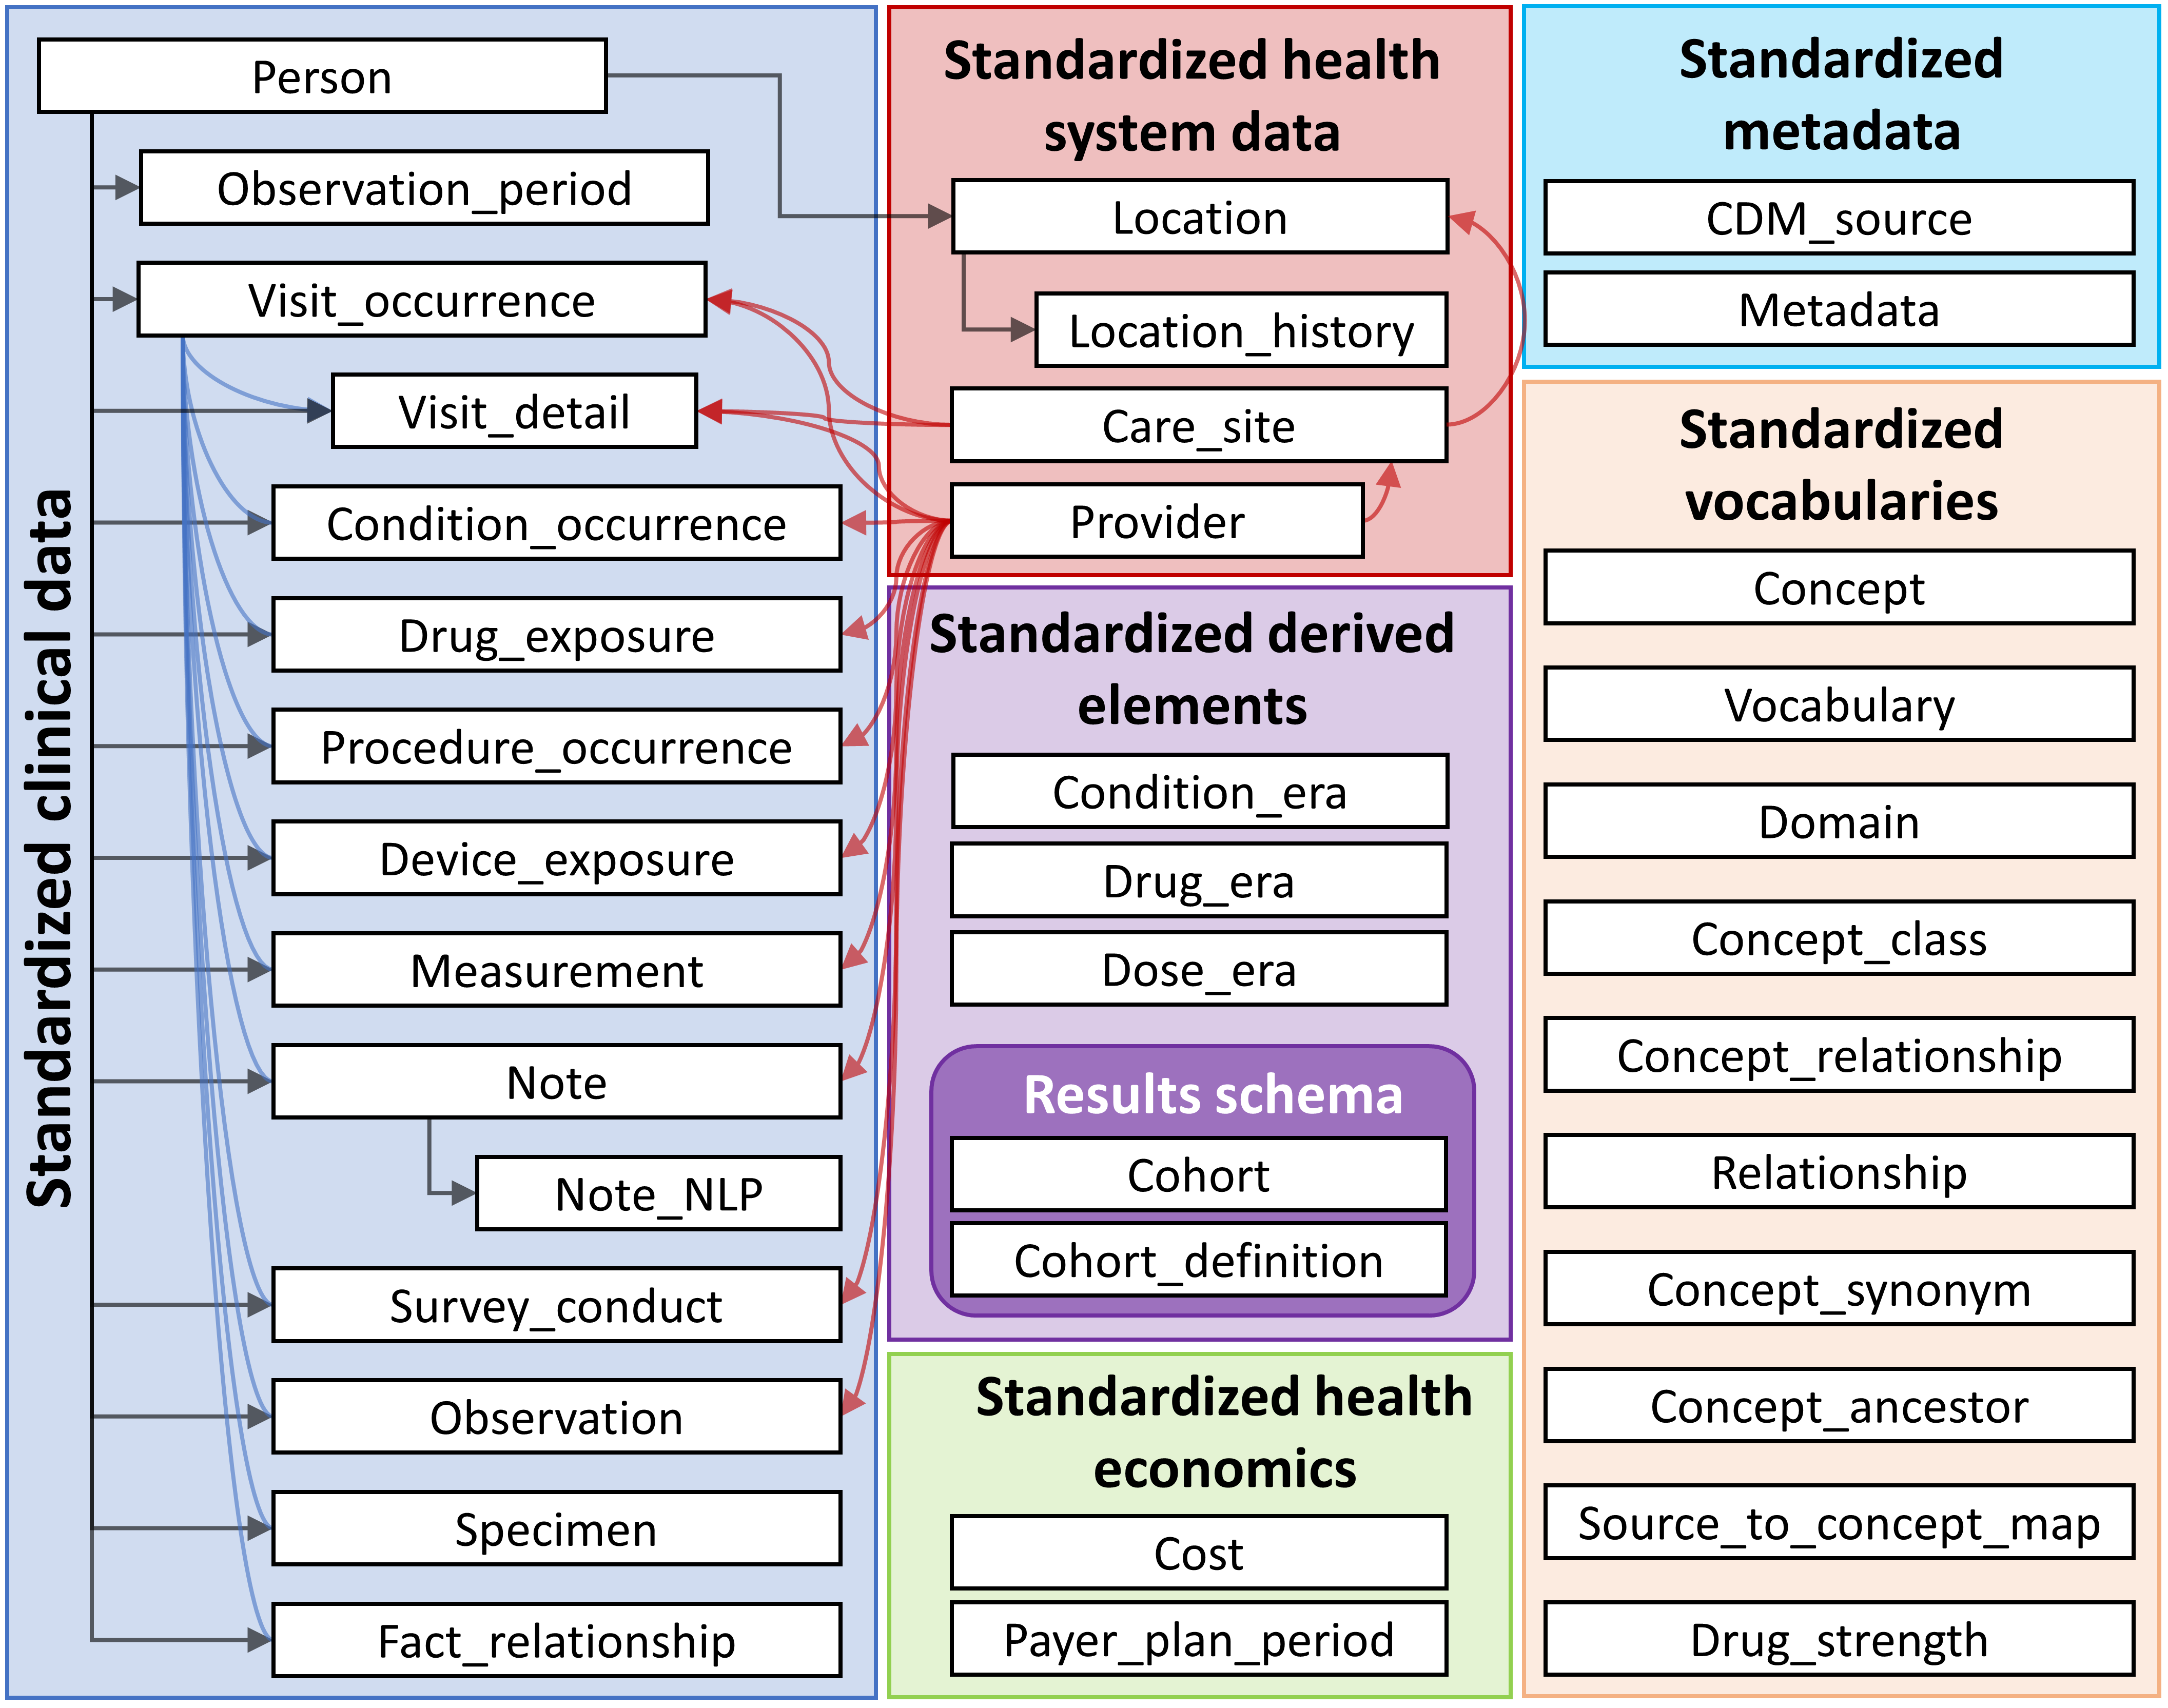
\includegraphics[width=1\linewidth]{images/CommonDataModel/cdmDiagram} \caption{CDM 6.0 버전의 모든 테이블에 대한 개요. 테이블 간의 모든 관계가 묘사되어 있는 것은 아니다.}\label{fig:cdmDiagram}
\end{figure}

\section{설계 원리}\label{-}

CDM은 다음과 같은 전형적인 관찰 연구 목적에 최적화되어
있다.\index{Common Data Model!design principles}

\begin{itemize}
\tightlist
\item
  특정한 의료 행위의 개입(약물 노출, 시술(procedure), 의료 정책 변경
  등)이 있거나 의료 관련 결과(질환, 시술(procedure), 기타 약물 노출에
  대한)를 포함하는 환자 집단 확인.
\item
  인구 통계학적 정보, 질병의 자연사, 의료 서비스 전달, 활용 및 비용,
  병적 상태, 치료 및 치료 과정 등과 같은 다양한 매개 변수에 대한 환자
  집단의 특성 확인.
\item
  개별 환자에서 결과들의 발생 예측 - \ref{PatientLevelPrediction}장
  참고,
\item
  앞서 설명한 의료 행위의 개입들이 인구에 미치는 영향 추정 -
  \ref{PopulationLevelEstimation}장 참고,
\end{itemize}

이러한 목표를 달성하기 위해서 CDM의 개발은 다음과 같은 설계 요소를
따른다:

\begin{itemize}
\tightlist
\item
  \textbf{목적에 대한 적합성}: CDM은 의료 서비스 제공자 혹은 지불인의
  운영 요구를 해결하기 위한 목적 보다는 분석에 최적화된 방식으로 구성된
  데이터를 제공하는 것을 목표로 한다.
  \index{Common Data Model!suitability for purpose}
\item
  \textbf{데이터 보호}: 이름, 생년월일 등 환자의 신원 및 안전을 위협할
  수 있는 모든 데이터는 제한되어 있다. 영아에 대한 연구를 위한 정확한
  생년 월일과 같은 보다 자세한 정보가 명시적으로 필요한 경우에는 예외가
  가능하다.\index{Common Data Model!data protection}
\item
  \textbf{도메인 설계}: 도메인은 개인 중심 관계형 데이터
  모델(person-centric relational data model)로 모델링 되며 각 기록마다
  개인의 신원과 날짜 정보가 최소한으로 수집된다. 여기서 관계형 데이터
  모델은 데이터가 기본 키와 외래 키로 연결된 테이블의 모음으로 표현되는
  모델이다.
\item
  \textbf{도메인의 이론적 근거}: 개체-관계 모델(entity-relationship
  model)에서 도메인은 분석 이용 사례가 있는지 (예를 들면,
  질환(conditions)) 그리고 달리 적용 가능한 방안이 없는 특정한
  속성(attributes)이 있는지에 따라 식별되고 별도로 정의된다. 다른 모든
  데이터는 개체-속성-값 구조(entity-attribute-value structure)의
  Observation 테이블에 관찰 데이터로 보존될 수 있다.
  \index{Common Data Model!domains}
\item
  \textbf{표준화된 어휘}: 기록들의 내용을 표준화하기 위해, CDM은 모든
  필수적이고 적절한 표준 건강 관리 개념(concept)을 포함하는 표준화된
  어휘에 의존한다.
\item
  \textbf{기존 어휘 재사용}: 이러한 개념은 국립 의학 도서관, 재향 군인
  담당 부서, 질병 통제 및 예방 센터 등과 같은 국가 및 산업 표준화 또는
  용어 정의 주도 기관이나 협회에서 활용되기도 한다.
\item
  \textbf{원본 코드 유지 관리}: 모든 코드가 표준화된 어휘에
  매핑(mapping)되어 있더라도 정보가 소실되지 않도록 원본 코드도
  저장한다. \index{Common Data Model!Source Codes}
  \index{Common Data Model!data loss prevention}
\item
  \textbf{기술 중립성}: CDM에는 특정한 기술을 필요로 하지 않는다.
  Oracle, SQL Server 등과 같은 관계형 데이터베이스 또는 SAS 분석 데이터
  세트로 구현될 수 있다. \index{Common Data Model!technology neutrality}
\item
  \textbf{확장성}: CDM은 데이터 처리 및 계산 분석에 최적화되어 있기
  때문에 수 억 명에 이르는 데이터베이스와 수 십 억 건에 달하는 임상
  관찰을 비롯한 데이터 베이스의 크기가 다양한 원천 데이터를 수용할 수
  있다. \index{Common Data Model!scalability}
\item
  \textbf{이전 버전과의 호환성}: 이전 CDM로부터의 모든 변경 사항은
  github 저장소
  \href{https://github.com/OHDSI/CommonDataModel}{(https://github.com/OHDSI/CommonDataModel)}에
  명확하게 서술되어 있다. CDM의 이전 버전은 현재 버전을 이용해 쉽게 만들
  수 있으며, 이전에 있었던 정보는 손실되지 않는다.
  \index{Common Data Model!backwards compatibility}
\end{itemize}

\section{데이터 모델 규칙}\label{--}

CDM에 채택된 많은 암시적 혹은 명시적인 규칙이 있다. CDM에 관련한 메소드
개발자들은 이러한 규칙들을 이해하고 있어야 한다.
\index{Common Data Model!conventions}

\subsection{모델의 일반적인 규칙}\label{model-Conv}

CDM은 ``개인 중심''모델로서, 모든 임상적인 사건에 대한 테이블이 PERSON
테이블에 연결되어 있다. 시작 날짜 및 기타 날짜 정보들과 더불어 이는 모든
의료 관련 사건에 대해 각 사람별로 종적 관찰이 가능하도록 한다. 이러한
규칙들의 예외 사항은 다양한 도메인의 사건들에 직접 연결되는 표준화된
의료 체계의 데이터 테이블들이다.

\subsection{스키마의 일반적인 규칙}\label{--}

스키마 또는 데이터베이스의 사용자는 읽기 전용 테이블과 읽기/쓰기
테이블을 분리할 수 있다. 임상 사건 및 어휘 테이블은 ``CDM'' 스키마에
저장되어 있으며 최종 사용자 또는 분석 도구에서는 읽기 전용으로 이용된다.
웹 기반 도구 및 최종 사용자에 의해 조작될 필요가 있는 테이블은 ``결과''
스키마에 저장된다. ``결과'' 스키마의 두 테이블은 COHORT와
COHORT\_DEFINITON이다. 이 테이블들은 \ref{Cohorts} 장에 자세히 설명되어
있는 것처럼 사용자가 정의할 수 있는 관심 그룹을 설명하기 위한 것이다.
이는 런타임 동안에 테이블이 작성될 수 있음을, 즉 코호트가 COHORT
테이블에 저장될 수 있다는 것을 의미한다. 모든 사용자를 위한 읽기-쓰기
스키마는 단 하나뿐이므로, 여러 사용자 접근이 어떻게 구성되고
제어되는지는 CDM의 구현에 달려 있다.

\subsection{데이터 테이블의 일반적인 규칙}\label{---}

CDM은 플랫폼에 비의존적이다. 데이터 유형은 일반적으로 ANSI SQL 데이터
유형(VARCHAR, INTEGER, FLOAT, DATE, DATETIME, CLOB)을 사용하여 정의된다.
VARCHAR에서만 정밀도가 제공된다. 이는 필요한 최소 문자열 길이를
반영하지만 구체적인 CDM 인스턴스화 내에서 확장될 수 있다. CDM은 날짜 및
날짜시간 형식을 규정하지 않는다. CDM에 대한 표준 쿼리는 로컬 인스턴스 및
날짜/시간 구성에 따라 달라질 수 있다.

\emph{참고}: 데이터 모델 자체는 플랫폼에 독립적이지만, 데이터 모델과
함께 작동하도록 구축된 여러 도구는 특정 사양이 요구된다. 이에 대한
자세한 내용은 \ref{OhdsiAnalyticsTools}장을 참조.

\subsection{도메인의 일반적인 규칙}\label{domains}

서로 다른 성격의 사건들은 도메인에 정리되어 있다. 이러한 사건들은
도메인별로 테이블과 필드에 저장되고, 표준화된 어휘에 정의되어 있는 대로
도메인별 표준 Concept으로 표현된다(\ref{conceptDomains} 참조). 각 표준
Concept에 고유한 도메인 할당이 되는데, 이는 어떤 테이블에 기록되는지를
정의한다. 정확한 도메인 할당이 커뮤니티내에서 항상 논의의 대상이 되지만,
엄격한 도메인-테이블-필드간 대응 규칙은 어떤 코드나 Concept에 대해서도
항상 모호한 위치는 없음을 보장한다. 예를 들어, 증상 및 진단 Concept은
Condition 도메인에 속하며 Condition\_OCCURRENCE
테이블의CONDITION\_CONCEP\_ID로 기록된다. 소위 말하는 시술약품은
일반적으로 원천 데이터의 Procedure 테이블에 Procedure 코드로 기록된다.
CDM에서 이러한 정보들은 매핑된 표준 Concept이 약물 도메인에 할당
되어있기 때문에 DRUG\_EXPOSURE 테이블에서 찾을 수 있다. 표
\ref{tab:domains}과 같이 총 30개의 도메인이 있다.

\begin{longtable}[]{@{}llll@{}}
\caption{\label{tab:domains} 각 도메인에 속하는 표준 Concept의
수.}\tabularnewline
\toprule
Concept Count & Domain ID & Concept Count & Domain ID\tabularnewline
\midrule
\endfirsthead
\toprule
Concept Count & Domain ID & Concept Count & Domain ID\tabularnewline
\midrule
\endhead
1731378 & Drug & 183 & Route\tabularnewline
477597 & Device & 180 & Currency\tabularnewline
257000 & Procedure & 158 & Payer\tabularnewline
163807 & Condition & 123 & Visit\tabularnewline
145898 & Observation & 51 & Cost\tabularnewline
89645 & Measurement & 50 & Race\tabularnewline
33759 & Spec Anatomic Site & 13 & Plan Stop Reason\tabularnewline
17302 & Meas Value & 11 & Plan\tabularnewline
1799 & Specimen & 6 & Episode\tabularnewline
1215 & Provider Specialty & 6 & Sponsor\tabularnewline
1046 & Unit & 5 & Meas Value Operator\tabularnewline
944 & Metadata & 3 & Spec Disease Status\tabularnewline
538 & Revenue Code & 2 & Gender\tabularnewline
336 & Type Concept & 2 & Ethnicity\tabularnewline
194 & Relationship & 1 & Observation Type\tabularnewline
\bottomrule
\end{longtable}

\subsection{Concept을 통한 내용의 표현}\label{concept---}

CDM 데이터의 테이블에서는 각 정보의 내용이 완전히 정규화되어 Concept으로
표현된다. Concept은 CONCEPT 테이블의 외래 키 역할을 하는 각각의
CONCEPT\_ID 값이 할당되어 사건 테이블에 저장되며, 모든 CDM의
인스턴스들은 Concept에 대한 참고 자료로써 공통 데이터 모델과 함께
상호운용의 핵심 메커니즘이자 OHDSI 연구 네트워크의 기반인 동일한 CONCEPT
테이블을 사용한다. 표준 Concept이 없거나 식별되지 않는 경우에는
CONCEPT\_ID가 존재하지 않는 Concept이거나 알 수 없음 또는 매핑이
불가능함을 의미하는 0으로 설정된다.

CONCEPT 테이블의 정보들은 각각의 Concept에 대한 상세 정보(이름, 도메인,
클래스 등)를 포함하고 있다. Concepts, Concept Relationships, Concept
Ancestors 및 다른 Concept과 관련 있는 정보들은 표준화된 용어에 포함되어
있다(\ref{StandardizedVocabularies}장 참조).

\subsection{필드 명명 규칙}\label{--}

모든 테이블의 변수명은 하나의 규칙을 따른다:

\begin{longtable}[]{@{}ll@{}}
\caption{\label{tab:fieldConventions} 필드 명 규칙.}\tabularnewline
\toprule
\begin{minipage}[b]{0.34\columnwidth}\raggedright\strut
Notation\strut
\end{minipage} & \begin{minipage}[b]{0.60\columnwidth}\raggedright\strut
Description\strut
\end{minipage}\tabularnewline
\midrule
\endfirsthead
\toprule
\begin{minipage}[b]{0.34\columnwidth}\raggedright\strut
Notation\strut
\end{minipage} & \begin{minipage}[b]{0.60\columnwidth}\raggedright\strut
Description\strut
\end{minipage}\tabularnewline
\midrule
\endhead
\begin{minipage}[t]{0.34\columnwidth}\raggedright\strut
{[}Event{]}\_ID\strut
\end{minipage} & \begin{minipage}[t]{0.60\columnwidth}\raggedright\strut
각 행의 고유 식별자로, 사건 테이블간 관계를 설정하는 외래 키 역할을
한다. 예를 들어 PERSON\_ID는 각 개인을 고유하게 식별한다.
VISIT\_OCCURRENCE\_ID는 방문을 고유하게 식별한다.\strut
\end{minipage}\tabularnewline
\begin{minipage}[t]{0.34\columnwidth}\raggedright\strut
{[}Event{]}\_CONCEPT\_ID\strut
\end{minipage} & \begin{minipage}[t]{0.60\columnwidth}\raggedright\strut
CONCEPT 참고 테이블의 표준 Concept에 대한 외래 키. 이는 모든 표준화된
분석에 기본 기반이 되는 사건의 주요 표현이다. 예를 들어
CONDITION\_CONCEPT\_ID =
\href{http://athena.ohdsi.org/search-terms/terms/31967}{31967}에는
SNOMED Concept인 ``Nausea''에 대한 참조 값을 포함하고 있다.\strut
\end{minipage}\tabularnewline
\begin{minipage}[t]{0.34\columnwidth}\raggedright\strut
{[}Event{]}\_SOURCE \_CONCEPT\_ID\strut
\end{minipage} & \begin{minipage}[t]{0.60\columnwidth}\raggedright\strut
CONCEPT 참고 테이블의 행에 대한 외래 키. 이 Concept은 원본 값(아래)과
동등하며, 이때 {[}EVENT\_CONCEPT\_ID{]}와 동일한 표준 개념이거나 또 다른
비-표준 concept일 수 있다. 예를 들어, Condition\_SOURCE\_CONCEPT\_ID =
\href{http://athena.ohdsi.org/search-terms/terms/45431665}{45431665}는
독해용 용어의 ``Nausea'' 개념을 나타내며, 유사한
CONDITION\_CONCEPT\_ID는 표준 SNOMED-CT concept으로
\href{http://athena.ohdsi.org/search-terms/terms/31967}{31967}이다. 표준
Concept만이 사건의 의미를 모호하지 않게 표현하므로 표준 분석에 응용 시
상호 운용성이 없는 원본 개념을 사용하는 것은 바람직하지 않다.\strut
\end{minipage}\tabularnewline
\begin{minipage}[t]{0.34\columnwidth}\raggedright\strut
{[}Event{]}\_TYPE\_CONCEPT\_ID\strut
\end{minipage} & \begin{minipage}[t]{0.60\columnwidth}\raggedright\strut
표준화된 용어를 표준화되어 있고 원본 정보의 출처를 나타내는 CONCEPT 참고
테이블의 행에 대한 외래 키. 이는 사건의 유형이나 concept의 유형을
나타내는 것이 아니라 이 기록를 생성한 메커니즘에 대한 정보를 수집하는
것을 의미한다. 예를 들면, DRUG\_TYPE\_CONCEPT\_ID는 이 기록이 약국에서의
처방 (``Pharmacy dispensing'')으로 부터 발생하였는지 혹은 전자 처방
신청서 (``Prescription written'')로부터 발생하였는지를 구분한다.\strut
\end{minipage}\tabularnewline
\begin{minipage}[t]{0.34\columnwidth}\raggedright\strut
{[}Event{]}\_SOURCE\_VALUE\strut
\end{minipage} & \begin{minipage}[t]{0.60\columnwidth}\raggedright\strut
이 사건이 원천 데이터에 표현되어 있는 방식을 쓰여진 그대로의 코드 혹은
자유 텍스트 문자열이다. 이 원본 값들은 데이터 원본간에 통일되어 있지
않으므로 표준 분석 방식에 사용하는 것은 좋지 않다. 예를 들면,
CONDITION\_SOURCE\_VALUE는 ICD-9 코드 787.02에 점을 제외하고
``78702''라는 기록를 포함할 수 있다.\strut
\end{minipage}\tabularnewline
\bottomrule
\end{longtable}

\subsection{concept과 원본 값과의 차이}\label{concepts-Sources}

많은 테이블이 원본 값, 원본 concept, 표준 concept으로 다양한 위치에
동일한 정보를 포함하고 있다.

\begin{itemize}
\tightlist
\item
  \textbf{Source Values} 은 원천 데이터에서의 사건 기록의 본래의
  표현이다. 이는 ICD9CM, NDC 또는 Read와 같은 널리 사용되는 공공
  도메인의 코딩 시스템이나 CPT4, GPI 또는 MedDRA와 같이 독점적인 코딩
  시스템, 혹은 남성은 M 여성은 F와 같이 원천 데이터에서만 사용되는
  제한된 어휘의 코드일 수 있다. 또한 표준화 및 제어되지 않은 짧은 자유
  텍스트 문구 일 수도 있다. 원본 값은 데이터 테이블의 {[}Event{]}
  \_SOURCE\_VALUE 필드에 저장됩니다. concept은 임상적 요소의 의미를
  일반화하는 CDM 특이적인 개체이다. 대부분의 concept은 이미 의료계에
  존재하는 공개되었거나 독점적인 코딩 체계를 기반으로 하고 있지만,
  일부는 새롭게 생성되었다 (CONCEPT\_CODE는 ``OMOP''으로부터 시작됨).
  concept은 모든 도메인에 걸쳐 고유한 ID를 가지고 있다.
\item
  \textbf{Concepts} 은 임상적 요소의 의미를 일반화하는 CDM 특이적인
  개체이다. 대부분의 concept은 이미 의료계에 존재하는 공개되었거나
  독점적인 코딩 체계를 기반으로 하고 있지만, 일부는 새롭게 생성되었다
  (CONCEPT\_CODE는 ``OMOP''으로부터 시작됨). concept은 모든 도메인에
  걸쳐 고유한 ID를 가지고 있다.
\item
  \textbf{Source Concepts} 은 원 자료에서 사용된 코드를 나타내는
  concept이다. 원본 concept은 OMOP기반의 concept이 아니라 기존에
  존재하는 공개되었거나 독점적인 코딩 체계만을 위해 사용한다. 원본
  concept은 데이터 테이블의 {[}Event{]} \_SOURCE\_CONCEPT\_ID 필드에
  저장된다.
\item
  \textbf{Standard Concepts} 은 모든 데이터 베이스에서 고유하게 임상적인
  개체의 의미를 정의하는 데에 사용되고 원본에서 사용한 코딩 체계와는
  독립적인 concept이다. 표준 concept은 일반적으로 이미 공개되어 있거나
  독점적인 용어 원본에서 가져온다. 표준 concept과 동일한 의미를 가진 비
  표준 concept은 표준 용어의 표준 concept에 매핑되어 있다. 표준
  concept은 데이터 테이블의 {[}Event{]} \_CONCEPT\_ID 필드에서 참조된다.
\end{itemize}

원본 값은 편의 및 품질 보증 (Quality Assurance, QA) 목적으로만 제공된다.
여기에는 특정 데이터 원본의 맥락에서만 의미 있는 정보가 포함될 수 있다.
원본 값이나 원본 concept을 사용하는 것은 선택사항이지만, 원본 데이터가
코딩 시스템을 사용하는 경우 \textbf{강력하게 권장}된다. 하지만 표준
concept의 경우 \textbf{필수 사항}이다. 이 표준 concept을 필수적으로
사용하면 모든 CDM 인스턴스가 동일한 언어를 사용할 수 있다. 예를 들면
``Pulmonary Tuberculosis'' (TB, Figure \ref{fig:pulmTubICD9})의
condition은 TB에 대한 ICD9CM 코드가 011임을 나타낸다.

\begin{figure}

{\centering 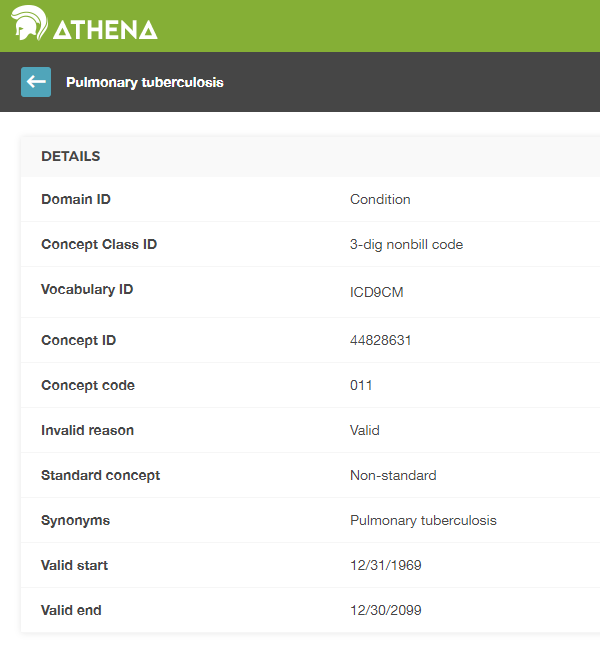
\includegraphics[width=0.75\linewidth]{images/CommonDataModel/pulmTubICD9} 

}

\caption{Pulmonary Tuberculosis의 ICD9CM 코드}\label{fig:pulmTubICD9}
\end{figure}

문맥이 없으면, 코드 011은 UB04 언어의 ``Hospital Inpatient (Including
Medicare Part A)''로 해석되거나, DRG 용어의 ``Nervous System Neoplasms
without Complications, Comorbidities''로 해석될 수 있다. 이것이 원본와
표준 모두의 concept ID가 중요한 이유이다. 011인 ICD9CM 코드를 나타내는
CONCEPT\_ID 값은
\href{http://athena.ohdsi.org/search-terms/terms/44828631}{44828631}이다.
이는 ICD9CM을 UBO4 및 DRG와 구별한다. ICD9CM의 TB 원본 concept은 그림
\ref{fig:pulmTubMap}과 같이``OMOP (Non-standard to Standard Map)''관계를
통해 SNOMED 어휘에서 표준 concept
\href{http://athena.ohdsi.org/search-terms/terms/253954}{253954}로
매핑된다. 표준 SNOMED 개념을 참조하는 모든 연구가 지원되는 모든 원본
코드를 포함할 수 있도록 Read, ICD10, CIEL 및 MeSH 코드에도 동일한 매핑
관계가 존재한다.

\begin{figure}
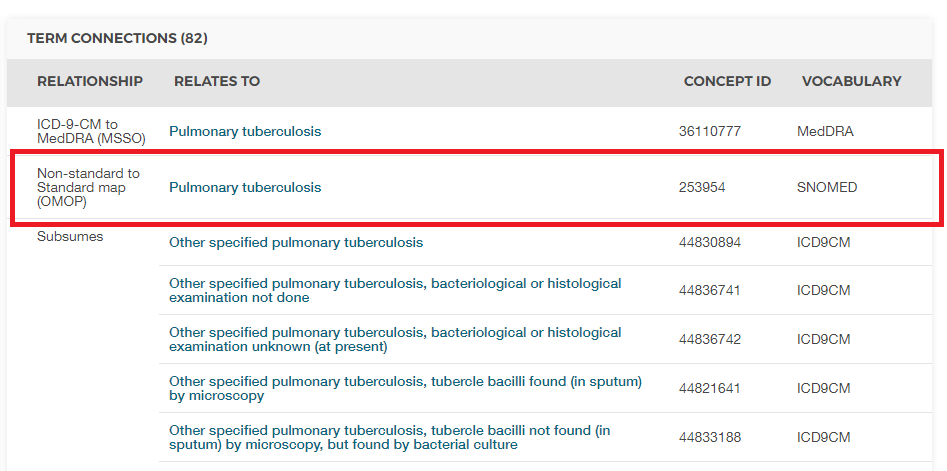
\includegraphics[width=1\linewidth]{images/CommonDataModel/pulmTubMap} \caption{Pulmonary Tuberculosis의 SNOMED 코드}\label{fig:pulmTubMap}
\end{figure}

표준 concept과 원본 concept의 관계를 보여주는 예가
표\ref{tab:conditionOccurrence}에 나와있다.

\section{표준화된 CDM 테이블}\label{-cdm-}

\index{Common Data Model!standardized tables}

DM에는 16개의 임상 사건 테이블, 10개의 어휘 테이블, 2개의 메타데이터
테이블, 4개의 보건 시스템 데이터 테이블, 2개의 보건 경제학 데이터
테이블, 3개의 표준화된 파생 요소 및 2개의 결과 스키마 테이블이 포함되어
있다. 이 테이블들은 CDM Wiki에 전체 명시되어 있다.\footnote{\url{https://github.com/OHDSI/CommonDataModel/wiki}}

이러한 테이블들이 실제로 어떻게 사용되는지를 설명하기 위해, 한 사람의
데이터를 이 장의 나머지 부분에서 걸쳐 공통으로 사용할 것이다.

\subsection{실행 예제: 자궁내막증}\label{--}

자궁내막증은 보통 여성의 자궁 안쪽에서 발견되는 세포가 신체 다른 곳에서
생겨나는 고통스러운 질환이다. 심한 경우는 불임, 장, 방광 문제를 일으킬
수 있다. 해당 섹션에서는 한 환자의 이 질병에 대한 경험과 이 질병이 공통
데이터 모델로 어떻게 표현되는지를 상세하게 설명하고자 한다.

\begin{center}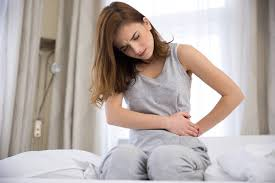
\includegraphics[width=0.5\linewidth]{images/CommonDataModel/Lauren} \end{center}

\begin{quote}
나는 이 고통스러운 여정의 모든 과정마다 내가 얼마만큼의 고통을 받고
있는지를 모두에게 납득시켜야 했다.
\end{quote}

Lauren은 수년 동안 자궁 내막증 증상을 겪어 왔다. 그러나 진단을 받기 전에
난소에서 낭종이 파열되었다. Lauren에 대한 자세한 내용은
\url{https://www.endometriosis-uk.org/laurens-story}에서 확인할 수 있다.

\subsection{PERSON 테이블}\label{person}

\subsubsection*{Lauren에 대해서 우리가 알고 있는
것은?}\label{lauren-----}
\addcontentsline{toc}{subsubsection}{Lauren에 대해서 우리가 알고 있는
것은?}

\begin{itemize}
\tightlist
\item
  그녀는 36세 여성이다
\item
  그녀의 생년월일은 1982년 3월 12일이다
\item
  그녀는 백인이다
\item
  그녀는 영국인이다
\end{itemize}

이를 염두에 두면 PERSON 테이블을 다음과 같이 나타낼 수 있다:

\begin{longtable}[]{@{}lll@{}}
\caption{\label{tab:person} PERSON 테이블.}\tabularnewline
\toprule
\begin{minipage}[b]{0.28\columnwidth}\raggedright\strut
Column name\strut
\end{minipage} & \begin{minipage}[b]{0.16\columnwidth}\raggedright\strut
Value\strut
\end{minipage} & \begin{minipage}[b]{0.48\columnwidth}\raggedright\strut
Explanation\strut
\end{minipage}\tabularnewline
\midrule
\endfirsthead
\toprule
\begin{minipage}[b]{0.28\columnwidth}\raggedright\strut
Column name\strut
\end{minipage} & \begin{minipage}[b]{0.16\columnwidth}\raggedright\strut
Value\strut
\end{minipage} & \begin{minipage}[b]{0.48\columnwidth}\raggedright\strut
Explanation\strut
\end{minipage}\tabularnewline
\midrule
\endhead
\begin{minipage}[t]{0.28\columnwidth}\raggedright\strut
PERSON\_ID\strut
\end{minipage} & \begin{minipage}[t]{0.16\columnwidth}\raggedright\strut
1\strut
\end{minipage} & \begin{minipage}[t]{0.48\columnwidth}\raggedright\strut
PERSON\_ID는 원본에서 직접적으로 생성되거나 빌드 과정의 일부분으로
생성된 정수여야 한다.\strut
\end{minipage}\tabularnewline
\begin{minipage}[t]{0.28\columnwidth}\raggedright\strut
GENDER\_CONCEPT\_ID\strut
\end{minipage} & \begin{minipage}[t]{0.16\columnwidth}\raggedright\strut
8532\strut
\end{minipage} & \begin{minipage}[t]{0.48\columnwidth}\raggedright\strut
여성을 의미하는 concept ID는
\href{http://athena.ohdsi.org/search-terms/terms/8532}{8532}이다.\strut
\end{minipage}\tabularnewline
\begin{minipage}[t]{0.28\columnwidth}\raggedright\strut
YEAR\_OF\_BIRTH\strut
\end{minipage} & \begin{minipage}[t]{0.16\columnwidth}\raggedright\strut
1982\strut
\end{minipage} & \begin{minipage}[t]{0.48\columnwidth}\raggedright\strut
\strut
\end{minipage}\tabularnewline
\begin{minipage}[t]{0.28\columnwidth}\raggedright\strut
MONTH\_OF\_BIRTH\strut
\end{minipage} & \begin{minipage}[t]{0.16\columnwidth}\raggedright\strut
3\strut
\end{minipage} & \begin{minipage}[t]{0.48\columnwidth}\raggedright\strut
\strut
\end{minipage}\tabularnewline
\begin{minipage}[t]{0.28\columnwidth}\raggedright\strut
DAY\_OF\_BIRTH\strut
\end{minipage} & \begin{minipage}[t]{0.16\columnwidth}\raggedright\strut
12\strut
\end{minipage} & \begin{minipage}[t]{0.48\columnwidth}\raggedright\strut
\strut
\end{minipage}\tabularnewline
\begin{minipage}[t]{0.28\columnwidth}\raggedright\strut
BIRTH\_DATETIME\strut
\end{minipage} & \begin{minipage}[t]{0.16\columnwidth}\raggedright\strut
1982-03-12 00:00:00\strut
\end{minipage} & \begin{minipage}[t]{0.48\columnwidth}\raggedright\strut
시간을 정확히 알 수 없는 경우 자정으로 한다.\strut
\end{minipage}\tabularnewline
\begin{minipage}[t]{0.28\columnwidth}\raggedright\strut
DEATH\_DATETIME\strut
\end{minipage} & \begin{minipage}[t]{0.16\columnwidth}\raggedright\strut
\strut
\end{minipage} & \begin{minipage}[t]{0.48\columnwidth}\raggedright\strut
\strut
\end{minipage}\tabularnewline
\begin{minipage}[t]{0.28\columnwidth}\raggedright\strut
RACE\_CONCEPT\_ID\strut
\end{minipage} & \begin{minipage}[t]{0.16\columnwidth}\raggedright\strut
8527\strut
\end{minipage} & \begin{minipage}[t]{0.48\columnwidth}\raggedright\strut
백인을 의미하는 concept ID는
\href{http://athena.ohdsi.org/search-terms/terms/8527}{8527}이다.
영국인이라는 민족성은
\href{http://athena.ohdsi.org/search-terms/terms/4093769}{4093769}이다.
둘 다 해당할 경우 전자를 활용한다. 민족성은 ETHNICITY\_CONCEPT\_ID가
아닌 인종의 일부로써 여기에 저장된다.\strut
\end{minipage}\tabularnewline
\begin{minipage}[t]{0.28\columnwidth}\raggedright\strut
ETHNICITY\_CONCEPT\_ ID\strut
\end{minipage} & \begin{minipage}[t]{0.16\columnwidth}\raggedright\strut
38003564\strut
\end{minipage} & \begin{minipage}[t]{0.48\columnwidth}\raggedright\strut
이는 히스패닉을 다른 사람들과 구분하기 위해 사용되는 전형적인 미국식
표기법이다. 이 경우 영국인인 민족성은 RACE\_CONCEPT\_ID에 저장된다. 미국
이외의 지역에서는 사용되지 않는다.
\href{http://athena.ohdsi.org/search-terms/terms/38003564}{38003564}는
``히스패닉이 아님''을 나타낸다.\strut
\end{minipage}\tabularnewline
\begin{minipage}[t]{0.28\columnwidth}\raggedright\strut
LOCATION\_ID\strut
\end{minipage} & \begin{minipage}[t]{0.16\columnwidth}\raggedright\strut
\strut
\end{minipage} & \begin{minipage}[t]{0.48\columnwidth}\raggedright\strut
주소는 알려져 있지 않다.\strut
\end{minipage}\tabularnewline
\begin{minipage}[t]{0.28\columnwidth}\raggedright\strut
PROVIDER\_ID\strut
\end{minipage} & \begin{minipage}[t]{0.16\columnwidth}\raggedright\strut
\strut
\end{minipage} & \begin{minipage}[t]{0.48\columnwidth}\raggedright\strut
일차 진료 제공자는 알려져 있지 않다.\strut
\end{minipage}\tabularnewline
\begin{minipage}[t]{0.28\columnwidth}\raggedright\strut
CARE\_SITE\strut
\end{minipage} & \begin{minipage}[t]{0.16\columnwidth}\raggedright\strut
\strut
\end{minipage} & \begin{minipage}[t]{0.48\columnwidth}\raggedright\strut
일차 진료 장소는 알려져 있지 않다.\strut
\end{minipage}\tabularnewline
\begin{minipage}[t]{0.28\columnwidth}\raggedright\strut
PERSON\_SOURCE\_ VALUE\strut
\end{minipage} & \begin{minipage}[t]{0.16\columnwidth}\raggedright\strut
1\strut
\end{minipage} & \begin{minipage}[t]{0.48\columnwidth}\raggedright\strut
대부분 PERSON\_ID 와 동일 하지만 일반적으로 이는 원본 데이터에서의
그녀의 식별자가 될 것이다.\strut
\end{minipage}\tabularnewline
\begin{minipage}[t]{0.28\columnwidth}\raggedright\strut
GENDER\_SOURCE\_ VALUE\strut
\end{minipage} & \begin{minipage}[t]{0.16\columnwidth}\raggedright\strut
F\strut
\end{minipage} & \begin{minipage}[t]{0.48\columnwidth}\raggedright\strut
원본에 나타난 성별에 대한 값이 여기에 저장되어 있다.\strut
\end{minipage}\tabularnewline
\begin{minipage}[t]{0.28\columnwidth}\raggedright\strut
GENDER\_SOURCE\_ CONCEPT\_ID\strut
\end{minipage} & \begin{minipage}[t]{0.16\columnwidth}\raggedright\strut
0\strut
\end{minipage} & \begin{minipage}[t]{0.48\columnwidth}\raggedright\strut
원본의 성별에 대한 값이 OHDSI에서 지원하는 코딩 체계를 사용한 경우 해당
concept이 여기에 해당한다. 예를 들어, 그녀의 성별이 원본에서
``sex-F''이고 PCORNet 어휘 concept에 있다고 언급되어 있다면
\href{http://athena.ohdsi.org/search-terms/terms/44814665}{44814665}이
이 필드에 입력될 것이다.\strut
\end{minipage}\tabularnewline
\begin{minipage}[t]{0.28\columnwidth}\raggedright\strut
RACE\_SOURCE\_ VALUE\strut
\end{minipage} & \begin{minipage}[t]{0.16\columnwidth}\raggedright\strut
white\strut
\end{minipage} & \begin{minipage}[t]{0.48\columnwidth}\raggedright\strut
인종 값이 원본에 있는대로 여기에 저장된다.\strut
\end{minipage}\tabularnewline
\begin{minipage}[t]{0.28\columnwidth}\raggedright\strut
RACE\_SOURCE\_ CONCEPT\_ID\strut
\end{minipage} & \begin{minipage}[t]{0.16\columnwidth}\raggedright\strut
0\strut
\end{minipage} & \begin{minipage}[t]{0.48\columnwidth}\raggedright\strut
GENDER\_CONCEPT\_ID와 같은 원리 적용.\strut
\end{minipage}\tabularnewline
\begin{minipage}[t]{0.28\columnwidth}\raggedright\strut
ETHNICITY\_SOURCE\_ VALUE\strut
\end{minipage} & \begin{minipage}[t]{0.16\columnwidth}\raggedright\strut
english\strut
\end{minipage} & \begin{minipage}[t]{0.48\columnwidth}\raggedright\strut
민족성 값이 원본에 나와 있는대로 여기에 저장된다.\strut
\end{minipage}\tabularnewline
\begin{minipage}[t]{0.28\columnwidth}\raggedright\strut
ETHNICITY\_SOURCE\_ CONCEPT\_ID\strut
\end{minipage} & \begin{minipage}[t]{0.16\columnwidth}\raggedright\strut
0\strut
\end{minipage} & \begin{minipage}[t]{0.48\columnwidth}\raggedright\strut
GENDER\_SOURCE\_CONCEPT\_ID와 같은 원리 적용.\strut
\end{minipage}\tabularnewline
\bottomrule
\end{longtable}

\subsection{OBSERVATION\_PERIOD 테이블}\label{observationPeriod}

OBSERVATION\_PERIAD 테이블은 최소한 환자의 인구통계, 질환, 시술 및
약물이 원본 시스템에 기록되는 시간을 민감성과 특수성을 고려하여 합리적인
예상을 통해 정의하도록 설계되었다. 보험 데이터의 경우 일반적으로 환자의
등록 시기이다. 대부분의 의료 시스템이 어떤 의료 기관이나 제공업체를
방문할지 결정해두지 않기 때문에 전자 건강 기록(EHR)에서는 더욱 까다롭다.
차선책으로서 시스템의 첫 번째 기록은 관측 기간의 시작일로 간주되고 최신
기록은 종료일로 간주된다.

\subsubsection*{Lauren의 Observation Period은 어떻게
정의될까?}\label{lauren-observation-period--}
\addcontentsline{toc}{subsubsection}{Lauren의 Observation Period은
어떻게 정의될까?}

표 \ref{tab:encounters}에 나타난 Lauren의 정보가 EHR 시스템에
기록되었다고 가정하자. 그녀의 Observation period에서 얻어진 방문기록은
다음과 같다:

\begin{longtable}[]{@{}llll@{}}
\caption{\label{tab:encounters} Lauren의 의료 기관 방문.}\tabularnewline
\toprule
Encounter ID & Start date & Stop date & Type\tabularnewline
\midrule
\endfirsthead
\toprule
Encounter ID & Start date & Stop date & Type\tabularnewline
\midrule
\endhead
70 & 2010-01-06 & 2010-01-06 & outpatient\tabularnewline
80 & 2011-01-06 & 2011-01-06 & outpatient\tabularnewline
90 & 2012-01-06 & 2012-01-06 & outpatient\tabularnewline
100 & 2013-01-07 & 2013-01-07 & outpatient\tabularnewline
101 & 2013-01-14 & 2013-01-14 & ambulatory\tabularnewline
102 & 2013-01-17 & 2013-01-24 & inpatient\tabularnewline
\bottomrule
\end{longtable}

방문기록을 기반으로 했을 때 그녀의 OBSERVATION\_PERIOD 테이블은 다음과
같을 것이다:

\begin{longtable}[]{@{}lll@{}}
\caption{\label{tab:observationPeriod} OBSERVATION\_PERIOD
테이블.}\tabularnewline
\toprule
\begin{minipage}[b]{0.29\columnwidth}\raggedright\strut
Column name\strut
\end{minipage} & \begin{minipage}[b]{0.14\columnwidth}\raggedright\strut
Value\strut
\end{minipage} & \begin{minipage}[b]{0.48\columnwidth}\raggedright\strut
Explanation\strut
\end{minipage}\tabularnewline
\midrule
\endfirsthead
\toprule
\begin{minipage}[b]{0.29\columnwidth}\raggedright\strut
Column name\strut
\end{minipage} & \begin{minipage}[b]{0.14\columnwidth}\raggedright\strut
Value\strut
\end{minipage} & \begin{minipage}[b]{0.48\columnwidth}\raggedright\strut
Explanation\strut
\end{minipage}\tabularnewline
\midrule
\endhead
\begin{minipage}[t]{0.29\columnwidth}\raggedright\strut
OBSERVATION\_ PERIOD\_ID\strut
\end{minipage} & \begin{minipage}[t]{0.14\columnwidth}\raggedright\strut
1\strut
\end{minipage} & \begin{minipage}[t]{0.48\columnwidth}\raggedright\strut
이는 일반적으로 테이블의 각 기록에 대한 고유 식별자를 생성하는 자동으로
생성되는 값이다.\strut
\end{minipage}\tabularnewline
\begin{minipage}[t]{0.29\columnwidth}\raggedright\strut
PERSON\_ID\strut
\end{minipage} & \begin{minipage}[t]{0.14\columnwidth}\raggedright\strut
1\strut
\end{minipage} & \begin{minipage}[t]{0.48\columnwidth}\raggedright\strut
PERSON 테이블에서 Laura의 기록에 대한 외래 키이며 PERSON을
OBSERVATION\_PERIOD 테이블에 연결한다.\strut
\end{minipage}\tabularnewline
\begin{minipage}[t]{0.29\columnwidth}\raggedright\strut
OBSERVATION\_PERIOD\_ START\_DATE\strut
\end{minipage} & \begin{minipage}[t]{0.14\columnwidth}\raggedright\strut
2010-01-06\strut
\end{minipage} & \begin{minipage}[t]{0.48\columnwidth}\raggedright\strut
이는 기록상 그녀의 가장 처음 방문했을 때 시작 날짜이다.\strut
\end{minipage}\tabularnewline
\begin{minipage}[t]{0.29\columnwidth}\raggedright\strut
OBSERVATION\_PERIOD\_ END\_DATE\strut
\end{minipage} & \begin{minipage}[t]{0.14\columnwidth}\raggedright\strut
2013-01-24\strut
\end{minipage} & \begin{minipage}[t]{0.48\columnwidth}\raggedright\strut
이는 기록상 그녀의 가장 마지막 방문했을 때 마지막 날짜이다.\strut
\end{minipage}\tabularnewline
\begin{minipage}[t]{0.29\columnwidth}\raggedright\strut
PERIOD\_TYPE\_ CONCEPT\_ID\strut
\end{minipage} & \begin{minipage}[t]{0.14\columnwidth}\raggedright\strut
44814725\strut
\end{minipage} & \begin{minipage}[t]{0.48\columnwidth}\raggedright\strut
concept의 클래스가 ``Obs Period Type''인 어휘에서 가장 좋은 선택은
\href{http://athena.ohdsi.org/search-terms/terms/44814724}{44814724}이며,
이는 ``의료 관련 방문 기간(Period covering healthcare encounters)''을
나타냅니다.\strut
\end{minipage}\tabularnewline
\bottomrule
\end{longtable}

\subsection{VISIT\_OCCURRENCE}\label{visitOccurrence}

VISIT\_OCCURRENCE에서는 환자의 의료 시스템에 방문한 정보에 대해 저장되어
있다. OHDSI 언어내에서 이를 Visit이라고 하며 주요한 사건로 간주한다.
의료 서비스가 제공될 수 있는 다양한 환경을 나타내는 광범위한 계층 구조를
가진 12 가지 주요 방문 카테고리가 있다. 가장 일반적인 Visit 기록는
입원(inpatient), 외래(outpatient), 응급실(emergency department) 및
비-의료 기관방문(non-medical institution Visits)이다.

\subsubsection*{Lauren의 방문을 Visit으로 어떻게 표현할 수
있을까?}\label{lauren--visit----}
\addcontentsline{toc}{subsubsection}{Lauren의 방문을 Visit으로 어떻게
표현할 수 있을까?}

예를 들어 VISIT\_OCCURRENCE 테이블의 표 \ref{tab:encounters}의 입원 환자
방문을 나타내어 보자.

\begin{longtable}[]{@{}lll@{}}
\caption{\label{tab:visitOccurrence} VISIT\_OCCURRENCE
테이블.}\tabularnewline
\toprule
\begin{minipage}[b]{0.28\columnwidth}\raggedright\strut
Column name\strut
\end{minipage} & \begin{minipage}[b]{0.16\columnwidth}\raggedright\strut
Value\strut
\end{minipage} & \begin{minipage}[b]{0.48\columnwidth}\raggedright\strut
Explanation\strut
\end{minipage}\tabularnewline
\midrule
\endfirsthead
\toprule
\begin{minipage}[b]{0.28\columnwidth}\raggedright\strut
Column name\strut
\end{minipage} & \begin{minipage}[b]{0.16\columnwidth}\raggedright\strut
Value\strut
\end{minipage} & \begin{minipage}[b]{0.48\columnwidth}\raggedright\strut
Explanation\strut
\end{minipage}\tabularnewline
\midrule
\endhead
\begin{minipage}[t]{0.28\columnwidth}\raggedright\strut
VISIT\_OCCURRENCE\_ ID\strut
\end{minipage} & \begin{minipage}[t]{0.16\columnwidth}\raggedright\strut
514\strut
\end{minipage} & \begin{minipage}[t]{0.48\columnwidth}\raggedright\strut
이는 일반적으로 테이블의 각 기록에 대한 고유 식별자를 생성하는 자동으로
생성되는 값이다.\strut
\end{minipage}\tabularnewline
\begin{minipage}[t]{0.28\columnwidth}\raggedright\strut
PERSON\_ID\strut
\end{minipage} & \begin{minipage}[t]{0.16\columnwidth}\raggedright\strut
1\strut
\end{minipage} & \begin{minipage}[t]{0.48\columnwidth}\raggedright\strut
PERSON 테이블에서 Laura의 기록에 대한 외래 키이며 PERSON을
VISIT\_OCCURRENCE에 연결한다.\strut
\end{minipage}\tabularnewline
\begin{minipage}[t]{0.28\columnwidth}\raggedright\strut
VISIT\_CONCEPT\_ID\strut
\end{minipage} & \begin{minipage}[t]{0.16\columnwidth}\raggedright\strut
9201\strut
\end{minipage} & \begin{minipage}[t]{0.48\columnwidth}\raggedright\strut
입원 환자 방문을 나타내는 외래 키는
\href{http://athena.ohdsi.org/search-terms/terms/9201}{9201}이다.\strut
\end{minipage}\tabularnewline
\begin{minipage}[t]{0.28\columnwidth}\raggedright\strut
VISIT\_START\_DATE\strut
\end{minipage} & \begin{minipage}[t]{0.16\columnwidth}\raggedright\strut
2013-01-17\strut
\end{minipage} & \begin{minipage}[t]{0.48\columnwidth}\raggedright\strut
Visit의 시작 날짜.\strut
\end{minipage}\tabularnewline
\begin{minipage}[t]{0.28\columnwidth}\raggedright\strut
VISIT\_START\_ DATETIME\strut
\end{minipage} & \begin{minipage}[t]{0.16\columnwidth}\raggedright\strut
2013-01-17 00:00:00\strut
\end{minipage} & \begin{minipage}[t]{0.48\columnwidth}\raggedright\strut
Visit의 날짜와 시간. 시간을 알 수 없기 때문에 자정으로 나타낸다.\strut
\end{minipage}\tabularnewline
\begin{minipage}[t]{0.28\columnwidth}\raggedright\strut
VISIT\_END\_DATE\strut
\end{minipage} & \begin{minipage}[t]{0.16\columnwidth}\raggedright\strut
2013-01-24\strut
\end{minipage} & \begin{minipage}[t]{0.48\columnwidth}\raggedright\strut
Visit의 종료 날짜. 일일 방문이라면 이 값이 시작 날짜와 동일해야
한다.\strut
\end{minipage}\tabularnewline
\begin{minipage}[t]{0.28\columnwidth}\raggedright\strut
VISIT\_END\_DATETIME\strut
\end{minipage} & \begin{minipage}[t]{0.16\columnwidth}\raggedright\strut
2013-01-24 00:00:00\strut
\end{minipage} & \begin{minipage}[t]{0.48\columnwidth}\raggedright\strut
Visit의 종료 날짜와 시간. 시간을 알 수 없기 때문에 자정으로
나타낸다.\strut
\end{minipage}\tabularnewline
\begin{minipage}[t]{0.28\columnwidth}\raggedright\strut
VISIT\_TYPE\_ CONCEPT\_ID\strut
\end{minipage} & \begin{minipage}[t]{0.16\columnwidth}\raggedright\strut
32035\strut
\end{minipage} & \begin{minipage}[t]{0.48\columnwidth}\raggedright\strut
이는 방문 기록의 보험 청구, 병원 청구, EHR 기록과 같은 제공처에 대한
정보를 제공한다. 해당 예에서는 방문 기록이 EHR과 유사하므로 concept ID
\href{http://athena.ohdsi.org/search-terms/terms/32035}{32035} (``Visit
derived from EHR encounter record'')이 사용되었다.\strut
\end{minipage}\tabularnewline
\begin{minipage}[t]{0.28\columnwidth}\raggedright\strut
PROVIDER\_ID*\strut
\end{minipage} & \begin{minipage}[t]{0.16\columnwidth}\raggedright\strut
NULL\strut
\end{minipage} & \begin{minipage}[t]{0.48\columnwidth}\raggedright\strut
방문 기록에 해당 제공자와 관련된 ID가 있을 경우 이 필드에 기록한다. 이는
PROVIDER 테이블의 PROVIDER\_ID 필드의 내용이어야 한다.\strut
\end{minipage}\tabularnewline
\begin{minipage}[t]{0.28\columnwidth}\raggedright\strut
CARE\_SITE\_ID\strut
\end{minipage} & \begin{minipage}[t]{0.16\columnwidth}\raggedright\strut
NULL\strut
\end{minipage} & \begin{minipage}[t]{0.48\columnwidth}\raggedright\strut
방문 기록에 치료 제공 장소와 관련된 ID가 있을 경우 이 필드에 기록한다.
이는 CARE\_SITE 테이블의 CARE\_SITE\_ID 필드의 내용이어야 한다.\strut
\end{minipage}\tabularnewline
\begin{minipage}[t]{0.28\columnwidth}\raggedright\strut
VISIT\_SOURCE\_ VALUE\strut
\end{minipage} & \begin{minipage}[t]{0.16\columnwidth}\raggedright\strut
inpatient\strut
\end{minipage} & \begin{minipage}[t]{0.48\columnwidth}\raggedright\strut
출처에 나와 있는 방문 값 그대로 여기에 입력한다. Lauren의 데이터에는
존재하지 않는다.\strut
\end{minipage}\tabularnewline
\begin{minipage}[t]{0.28\columnwidth}\raggedright\strut
VISIT\_SOURCE\_ CONCEPT\_ID\strut
\end{minipage} & \begin{minipage}[t]{0.16\columnwidth}\raggedright\strut
0\strut
\end{minipage} & \begin{minipage}[t]{0.48\columnwidth}\raggedright\strut
출처의 방문 값이 OHDSI에서 통용되는 용어를 사용하여 코딩 되어 있는 경우
원본 코드를 나타내는 CONCEPT\_ID 값을 여기에 넣는다. Lauren의 데이터에는
존재하지 않는다.\strut
\end{minipage}\tabularnewline
\begin{minipage}[t]{0.28\columnwidth}\raggedright\strut
ADMITTED\_FROM\_ CONCEPT\_ID\strut
\end{minipage} & \begin{minipage}[t]{0.16\columnwidth}\raggedright\strut
0\strut
\end{minipage} & \begin{minipage}[t]{0.48\columnwidth}\raggedright\strut
환자가 어디에서부터 입원해 왔는지 알 수 있는 경우 이를 나타내는
concept을 포함하고 있다. 이 concept은 ``Visit''의 도메인을 가지고 있어야
한다. 예를 들어 만약 환자가 집에서 병원으로 입원한 경우
\href{http://athena.ohdsi.org/search-terms/terms/8536}{8536}
(``Home'')값일 것이다.\strut
\end{minipage}\tabularnewline
\begin{minipage}[t]{0.28\columnwidth}\raggedright\strut
ADMITTED\_FROM\_ SOURCE\_CONCEPT\_ID\strut
\end{minipage} & \begin{minipage}[t]{0.16\columnwidth}\raggedright\strut
NULL\strut
\end{minipage} & \begin{minipage}[t]{0.48\columnwidth}\raggedright\strut
환자가 어디에서부터 입원해 왔는지를 나타내는 원본 값이다. 위의 예를
활용하면 여기에는 ``Home''이 들어가야 한다.\strut
\end{minipage}\tabularnewline
\begin{minipage}[t]{0.28\columnwidth}\raggedright\strut
DISCHARGE\_TO\_ CONCEPT\_ID\strut
\end{minipage} & \begin{minipage}[t]{0.16\columnwidth}\raggedright\strut
0\strut
\end{minipage} & \begin{minipage}[t]{0.48\columnwidth}\raggedright\strut
환자가 어디로 퇴원 되었는지 알 수 있는 경우 이를 나타내는 concept을
나타낸다. 이 concept은 ``Visit'' 도메인을 가지고 있어야 한다. 예를 들면,
만약 환자가 보조 생활 시설로 보내졌을 경우 concept ID는
\href{http://athena.ohdsi.org/search-terms/terms/8615}{8615} (``Assisted
Living Facility'')일 것이다.\strut
\end{minipage}\tabularnewline
\begin{minipage}[t]{0.28\columnwidth}\raggedright\strut
DISCHARGE\_TO\_ SOURCE\_VALUE\strut
\end{minipage} & \begin{minipage}[t]{0.16\columnwidth}\raggedright\strut
0\strut
\end{minipage} & \begin{minipage}[t]{0.48\columnwidth}\raggedright\strut
환자가 퇴원 한 곳을 나타내는 원본 값이다. 위의 예를 활용하면``보조 생활
시설''이 된다.\strut
\end{minipage}\tabularnewline
\begin{minipage}[t]{0.28\columnwidth}\raggedright\strut
PRECEDING\_VISIT\_ OCCURRENCE\_ID\strut
\end{minipage} & \begin{minipage}[t]{0.16\columnwidth}\raggedright\strut
NULL\strut
\end{minipage} & \begin{minipage}[t]{0.48\columnwidth}\raggedright\strut
현재 Visit의 바로 이전의 방문을 나타낸다. ADMITTED\_FROM\_CONCEPT\_ID와
달리 Visit Concept이 아닌 실제 Visit Occurrence 기록에 연결된다. 또한
Visit Occurrence에 따른 기록는 없으며 Visit Occurrence는 이 필드를
통해서만 연결되어 있다.\strut
\end{minipage}\tabularnewline
\bottomrule
\end{longtable}

\begin{itemize}
\tightlist
\item
  환자는 입원하는 경우와 마찬가지로 한번 방문하는 동안 여러 의료
  제공자와 상호 작용할 수 있다. 이러한 상호작용은 VISIT\_DETAIL 테이블에
  기록될 수 있다. 이 장에서는 자세히 다루지 않지만
  \href{https://github.com/OHDSI/CommonDataModel/wiki/VISIT_DETAIL}{CDM
  wiki}에서 VISIT\_DETAIL 테이블에 대한 자세한 내용을 확인할 수 있다.
\end{itemize}

\subsection{CONDITION\_OCCURRENCE}\label{conditionOccurrence}

CONDITION\_OCCURRENCE 테이블의 기록는 제공자가 관찰하거나 환자가 보고한
상태의 진단,징후 또는 증상이다.

\subsubsection*{Lauren의 condition은 무엇일까?}\label{lauren-condition-}
\addcontentsline{toc}{subsubsection}{Lauren의 condition은 무엇일까?}

그녀의 예로 돌아가자면 그녀는 다음과 같이 말한다:

\begin{quote}
3년 정도 전쯤 그 동안 매우 통증이 심했던 월경이 점점 더 고통스러워지고
있다는 것을 알아챘다. 나는 내 결장 바로 옆에서 날카롭게 쑤시는 통증을
느끼기 시작했고 꼬리뼈와 아랫골반 부위가 따갑고 부풀어 오르는 것을
느꼈다. 내 월경이 너무 고통스러워져서 일을 한달에 하루 이틀 쉬었다.
진통제가 가끔 고통을 줄여 주긴 했지만 보통은 그렇지 않았다.
\end{quote}

월경통이라고 하는 고통스러운 월경 경련의 SNOMED 코드는 266599000이다. 표
\ref{tab:conditionOccurrence} 은 CONDITION\_OCCURRENCE 테이블에 어떻게
표시되는 지를 보여준다:

\begin{longtable}[]{@{}lll@{}}
\caption{\label{tab:conditionOccurrence} CONDITION\_OCCURRENCE
테이블.}\tabularnewline
\toprule
\begin{minipage}[b]{0.28\columnwidth}\raggedright\strut
Column name\strut
\end{minipage} & \begin{minipage}[b]{0.16\columnwidth}\raggedright\strut
Value\strut
\end{minipage} & \begin{minipage}[b]{0.48\columnwidth}\raggedright\strut
Explanation\strut
\end{minipage}\tabularnewline
\midrule
\endfirsthead
\toprule
\begin{minipage}[b]{0.28\columnwidth}\raggedright\strut
Column name\strut
\end{minipage} & \begin{minipage}[b]{0.16\columnwidth}\raggedright\strut
Value\strut
\end{minipage} & \begin{minipage}[b]{0.48\columnwidth}\raggedright\strut
Explanation\strut
\end{minipage}\tabularnewline
\midrule
\endhead
\begin{minipage}[t]{0.28\columnwidth}\raggedright\strut
CONDITION\_ OCCURRENCE\_ID\strut
\end{minipage} & \begin{minipage}[t]{0.16\columnwidth}\raggedright\strut
964\strut
\end{minipage} & \begin{minipage}[t]{0.48\columnwidth}\raggedright\strut
이는 일반적으로 테이블의 각 기록에 대한 고유 식별자를 생성하는 자동으로
생성되는 값이다.\strut
\end{minipage}\tabularnewline
\begin{minipage}[t]{0.28\columnwidth}\raggedright\strut
PERSON\_ID\strut
\end{minipage} & \begin{minipage}[t]{0.16\columnwidth}\raggedright\strut
1\strut
\end{minipage} & \begin{minipage}[t]{0.48\columnwidth}\raggedright\strut
이는 PERSON 테이블에서 Laura의 기록에 대한 외래 키이며 PERSON을
CONDITION\_OCCURRENCE에 연결한다.\strut
\end{minipage}\tabularnewline
\begin{minipage}[t]{0.28\columnwidth}\raggedright\strut
CONDITION\_ CONCEPT\_ID\strut
\end{minipage} & \begin{minipage}[t]{0.16\columnwidth}\raggedright\strut
194696\strut
\end{minipage} & \begin{minipage}[t]{0.48\columnwidth}\raggedright\strut
SNOMED 코드 266599000을 나타내는 외래 키:
\href{http://athena.ohdsi.org/search-terms/terms/194696}{194696}.\strut
\end{minipage}\tabularnewline
\begin{minipage}[t]{0.28\columnwidth}\raggedright\strut
CONDITION\_START\_ DATE\strut
\end{minipage} & \begin{minipage}[t]{0.16\columnwidth}\raggedright\strut
2010-01-06\strut
\end{minipage} & \begin{minipage}[t]{0.48\columnwidth}\raggedright\strut
Condition의 인스턴스가 기록된 날짜이다.\strut
\end{minipage}\tabularnewline
\begin{minipage}[t]{0.28\columnwidth}\raggedright\strut
CONDITION\_START\_ DATETIME\strut
\end{minipage} & \begin{minipage}[t]{0.16\columnwidth}\raggedright\strut
2010-01-06 00:00:00\strut
\end{minipage} & \begin{minipage}[t]{0.48\columnwidth}\raggedright\strut
Condition의 인스턴스가 기록된 날짜 및 시간이다. 시간을 알 수 없으므로
자정으로 입력한다.\strut
\end{minipage}\tabularnewline
\begin{minipage}[t]{0.28\columnwidth}\raggedright\strut
CONDITION\_END\_ DATE\strut
\end{minipage} & \begin{minipage}[t]{0.16\columnwidth}\raggedright\strut
NULL\strut
\end{minipage} & \begin{minipage}[t]{0.48\columnwidth}\raggedright\strut
이는 인스턴스가 종료된 것으로 여겨지는 날짜지만 거의 기록되지
않는다.\strut
\end{minipage}\tabularnewline
\begin{minipage}[t]{0.28\columnwidth}\raggedright\strut
CONDITION\_END\_ DATETIME\strut
\end{minipage} & \begin{minipage}[t]{0.16\columnwidth}\raggedright\strut
NULL\strut
\end{minipage} & \begin{minipage}[t]{0.48\columnwidth}\raggedright\strut
Condition의 인스턴스가 종료된 것으로 여겨지는 날짜 및 시간이 알려져 있을
경우 입력한다.\strut
\end{minipage}\tabularnewline
\begin{minipage}[t]{0.28\columnwidth}\raggedright\strut
CONDITION\_TYPE\_ CONCEPT\_ID\strut
\end{minipage} & \begin{minipage}[t]{0.16\columnwidth}\raggedright\strut
32020\strut
\end{minipage} & \begin{minipage}[t]{0.48\columnwidth}\raggedright\strut
이 열은 기록의 출처, 즉 보험 청구, 병원 청구 기록, EHR 기록 등에서 얻어
졌다는 정보를 제공하기 위한 것이다. 해당 예에서는 방문 기록이 EHR과
유사하기 때문에 concept
\href{http://athena.ohdsi.org/search-terms/terms/32020}{32020} (``EHR
encounter diagnosis'')을 사용한다. 이 필드에 있는 concept은 ``Condition
Type''용어에 있는 것이여야 한다.\strut
\end{minipage}\tabularnewline
\begin{minipage}[t]{0.28\columnwidth}\raggedright\strut
CONDITION\_STATUS\_ CONCEPT\_ID\strut
\end{minipage} & \begin{minipage}[t]{0.16\columnwidth}\raggedright\strut
0\strut
\end{minipage} & \begin{minipage}[t]{0.48\columnwidth}\raggedright\strut
상황에 대해 알려진 것이 있을 경우 입력한다. 예를 들어, concept ID에
\href{http://athena.ohdsi.org/search-terms/terms/4203942}{4203942}가
사용되었을 경우 Condition이 인정된 진단명일 수 있다.\strut
\end{minipage}\tabularnewline
\begin{minipage}[t]{0.28\columnwidth}\raggedright\strut
STOP\_REASON\strut
\end{minipage} & \begin{minipage}[t]{0.16\columnwidth}\raggedright\strut
NULL\strut
\end{minipage} & \begin{minipage}[t]{0.48\columnwidth}\raggedright\strut
Condition이 더 이상 존재하지 않는 이유가 알려져 있으면 원본 데이터에
있는대로 입력한다.\strut
\end{minipage}\tabularnewline
\begin{minipage}[t]{0.28\columnwidth}\raggedright\strut
PROVIDER\_ID\strut
\end{minipage} & \begin{minipage}[t]{0.16\columnwidth}\raggedright\strut
NULL\strut
\end{minipage} & \begin{minipage}[t]{0.48\columnwidth}\raggedright\strut
만약 condition 기록에 진단의 제공자가 수록되어 있으면 해당 제공자의 ID를
이 필드에 입력한다. 이는 방문 시 제공자를 나타내는 PROVIDER 테이블의
PROVIDER\_ID의 내용이어야 한다.\strut
\end{minipage}\tabularnewline
\begin{minipage}[t]{0.28\columnwidth}\raggedright\strut
VISIT\_OCCURRENCE\_ ID\strut
\end{minipage} & \begin{minipage}[t]{0.16\columnwidth}\raggedright\strut
509\strut
\end{minipage} & \begin{minipage}[t]{0.48\columnwidth}\raggedright\strut
Condition이 진단되었을 당시 Visit값(VISIT\_OCCURRENCE 테이블의
VISIT\_OCCURRENCE\_ID에 대한 외래 키).\strut
\end{minipage}\tabularnewline
\begin{minipage}[t]{0.28\columnwidth}\raggedright\strut
CONDITION\_SOURCE\_ VALUE\strut
\end{minipage} & \begin{minipage}[t]{0.16\columnwidth}\raggedright\strut
266599000\strut
\end{minipage} & \begin{minipage}[t]{0.48\columnwidth}\raggedright\strut
Conditions을 나타내는 원래의 원본 값. Lauren의 월경 곤란의 사례에서는
해당 Condition에 대한 SNOMED 코드가 여기에 저장되고 코드를 나타내는
Concept은 CONDITION\_SOURCE\_CONCEPT\_ID로 이동했으며 이로부터 매핑된
표준 Concept은 CONDITION\_CONCEPT\_ID 필드에 저장된다.\strut
\end{minipage}\tabularnewline
\begin{minipage}[t]{0.28\columnwidth}\raggedright\strut
CONDITION\_SOURCE\_ CONCEPT\_ID\strut
\end{minipage} & \begin{minipage}[t]{0.16\columnwidth}\raggedright\strut
194696\strut
\end{minipage} & \begin{minipage}[t]{0.48\columnwidth}\raggedright\strut
원본의 질환 값이 OHDSI에서 활용하는 용어로 코드화되어 있을 경우 그 값을
나타내는 concept ID를 여기에 입력한다. 월경 곤란의 예에서는 그 원본 값이
SNOMED 코드 이므로 코드를 나타내는 Concept은 194696이다. 이 경우에서는
CONDITION\_CONCEPT\_ID 영역과 같은 값이다.\strut
\end{minipage}\tabularnewline
\begin{minipage}[t]{0.28\columnwidth}\raggedright\strut
CONDITION\_STATUS\_ SOURCE\_VALUE\strut
\end{minipage} & \begin{minipage}[t]{0.16\columnwidth}\raggedright\strut
0\strut
\end{minipage} & \begin{minipage}[t]{0.48\columnwidth}\raggedright\strut
원본의 질환의 상태 값이 OHDSI에서 지원하는 방식으로 코드화 되어 있을
경우 해당 concept을 여기에 입력한다.\strut
\end{minipage}\tabularnewline
\bottomrule
\end{longtable}

\subsection{DRUG\_EXPOSURE}\label{drugExposure}

DRUG\_EXPOSURE 테이블은 환자에 신체에 약물을 투여하고자 한 의도나 실제
투여에 대한 기록을 수집한다. 의약품에는 처방전이 필수적인 의약품과
처방전 없이 구입할 수 있는 의약품, 백신 및 고분자의 생물학적 제제를
포함한다. 약물 노출은 주문, 처방된 처방전, 약품 조제, 절차적 등록, 기타
환자가 보고한 정보와 같은 임상적인 사건에서 유추된다.

\subsubsection*{Lauren의 약물 노출은 어떻게 나타낼 수
있을까?}\label{lauren------}
\addcontentsline{toc}{subsubsection}{Lauren의 약물 노출은 어떻게 나타낼
수 있을까?}

월경 곤란 통증을 완화하기 위해 Lauren은 2010 년 1 월 6 일 방문하여 375mg
Acetaminophen (일명 Paracetamol, 미국 NDC 코드 69842087651) 경구 제제
60알을 30일치 받았다. 이는 DRUG\_EXPOSURE 테이블에서 다음과 같이
나타난다:

\begin{longtable}[]{@{}lll@{}}
\caption{\label{tab:drugExposure} DRUG\_EXPOSURE 테이블.}\tabularnewline
\toprule
\begin{minipage}[b]{0.28\columnwidth}\raggedright\strut
Column name\strut
\end{minipage} & \begin{minipage}[b]{0.16\columnwidth}\raggedright\strut
Value\strut
\end{minipage} & \begin{minipage}[b]{0.48\columnwidth}\raggedright\strut
Explanation\strut
\end{minipage}\tabularnewline
\midrule
\endfirsthead
\toprule
\begin{minipage}[b]{0.28\columnwidth}\raggedright\strut
Column name\strut
\end{minipage} & \begin{minipage}[b]{0.16\columnwidth}\raggedright\strut
Value\strut
\end{minipage} & \begin{minipage}[b]{0.48\columnwidth}\raggedright\strut
Explanation\strut
\end{minipage}\tabularnewline
\midrule
\endhead
\begin{minipage}[t]{0.28\columnwidth}\raggedright\strut
DRUG\_EXPOSURE\_ID\strut
\end{minipage} & \begin{minipage}[t]{0.16\columnwidth}\raggedright\strut
1001\strut
\end{minipage} & \begin{minipage}[t]{0.48\columnwidth}\raggedright\strut
이는 일반적으로 테이블의 각 기록에 대한 고유 식별자를 생성하는 자동으로
생성되는 값이다.\strut
\end{minipage}\tabularnewline
\begin{minipage}[t]{0.28\columnwidth}\raggedright\strut
PERSON\_ID\strut
\end{minipage} & \begin{minipage}[t]{0.16\columnwidth}\raggedright\strut
1\strut
\end{minipage} & \begin{minipage}[t]{0.48\columnwidth}\raggedright\strut
PERSON 테이블에서 Laura의 기록에 대한 외래 키이며 PERSON을
DRUG\_EXPOSURE에 연결한다.\strut
\end{minipage}\tabularnewline
\begin{minipage}[t]{0.28\columnwidth}\raggedright\strut
DRUG\_CONCEPT\_ID\strut
\end{minipage} & \begin{minipage}[t]{0.16\columnwidth}\raggedright\strut
1127433\strut
\end{minipage} & \begin{minipage}[t]{0.48\columnwidth}\raggedright\strut
의약품에 대한 개념. 아세트 아미노펜에 대한 NDC 코드는 Concept
\href{http://athena.ohdsi.org/search-terms/terms/1127433}{1127433}으로
표시되는 RxNorm 코드 313782에 매핑된다.\strut
\end{minipage}\tabularnewline
\begin{minipage}[t]{0.28\columnwidth}\raggedright\strut
DRUG\_EXPOSURE\_ START\_DATE\strut
\end{minipage} & \begin{minipage}[t]{0.16\columnwidth}\raggedright\strut
2010-01-06\strut
\end{minipage} & \begin{minipage}[t]{0.48\columnwidth}\raggedright\strut
약물에 노출되기 시작한 날짜.\strut
\end{minipage}\tabularnewline
\begin{minipage}[t]{0.28\columnwidth}\raggedright\strut
DRUG\_EXPOSURE\_ START\_DATETIME\strut
\end{minipage} & \begin{minipage}[t]{0.16\columnwidth}\raggedright\strut
2010-01-06 00:00:00\strut
\end{minipage} & \begin{minipage}[t]{0.48\columnwidth}\raggedright\strut
약물에 노출되기 시작한 날짜 및 시각. 알 수 없을 경우 자정을 입력\strut
\end{minipage}\tabularnewline
\begin{minipage}[t]{0.28\columnwidth}\raggedright\strut
DRUG\_EXPOSURE\_ END\_DATE\strut
\end{minipage} & \begin{minipage}[t]{0.16\columnwidth}\raggedright\strut
2010-02-05\strut
\end{minipage} & \begin{minipage}[t]{0.48\columnwidth}\raggedright\strut
약물 노출이 종료되는 날짜. 서로 다른 출처에서 알려져 있는 날짜나 추정된
날짜 일 수 있으며 환자가 약물에 노출 지속된 날짜의 마지막 날을 의미한다.
해당 사례에서는 Lauren이 30일 동안 제공받았음을 알기에 이 날짜가 추론될
수 있다.\strut
\end{minipage}\tabularnewline
\begin{minipage}[t]{0.28\columnwidth}\raggedright\strut
DRUG\_EXPOSURE\_ END\_DATETIME\strut
\end{minipage} & \begin{minipage}[t]{0.16\columnwidth}\raggedright\strut
2010-02-05 00:00:00\strut
\end{minipage} & \begin{minipage}[t]{0.48\columnwidth}\raggedright\strut
약물 노출 종료 날짜 및 시간. DRUG\_EXPOSURE\_END\_DATE와 비슷한 규칙이
적용된다. 알 수 없을 경우 자정을 입력.\strut
\end{minipage}\tabularnewline
\begin{minipage}[t]{0.28\columnwidth}\raggedright\strut
VERBATIM\_END\_DATE\strut
\end{minipage} & \begin{minipage}[t]{0.16\columnwidth}\raggedright\strut
NULL\strut
\end{minipage} & \begin{minipage}[t]{0.48\columnwidth}\raggedright\strut
원본에서 실제 종료 날짜를 명시한 경우, 환자가 전체 날짜에 약물에
노출되었다고 가정하여 유추되어 결정된다.\strut
\end{minipage}\tabularnewline
\begin{minipage}[t]{0.28\columnwidth}\raggedright\strut
DRUG\_TYPE\_ CONCEPT\_ID\strut
\end{minipage} & \begin{minipage}[t]{0.16\columnwidth}\raggedright\strut
38000177\strut
\end{minipage} & \begin{minipage}[t]{0.48\columnwidth}\raggedright\strut
해당 열은 보험 청구, 처방 기록 등에서 비롯된 기록의 출처에 대한 정보를
제공하기 위해 작성이 되었다. 이 예에서는 Concept
\href{http://athena.ohdsi.org/search-terms/terms/38000177}{38000177}
(``Prescription written'')이 사용되었다.\strut
\end{minipage}\tabularnewline
\begin{minipage}[t]{0.28\columnwidth}\raggedright\strut
STOP\_REASON\strut
\end{minipage} & \begin{minipage}[t]{0.16\columnwidth}\raggedright\strut
NULL\strut
\end{minipage} & \begin{minipage}[t]{0.48\columnwidth}\raggedright\strut
T약물 투여가 중단된 이유. 요법 완료, 변경 제거 등이 이유에 포함된다. 이
정보가 수집되는 경우는 거의 없다.\strut
\end{minipage}\tabularnewline
\begin{minipage}[t]{0.28\columnwidth}\raggedright\strut
REFILLS\strut
\end{minipage} & \begin{minipage}[t]{0.16\columnwidth}\raggedright\strut
NULL\strut
\end{minipage} & \begin{minipage}[t]{0.48\columnwidth}\raggedright\strut
대다수의 나라에서 처방 시스템의 일부인 초기 처방 이후 자동 재조제 횟수.
초기 처방은 세지 않고 NULL로 시작한다.Lauren의 아세트아미노펜의 경우
재조제되지 않았으므로 NULL이다.\strut
\end{minipage}\tabularnewline
\begin{minipage}[t]{0.28\columnwidth}\raggedright\strut
QUANTITY\strut
\end{minipage} & \begin{minipage}[t]{0.16\columnwidth}\raggedright\strut
60\strut
\end{minipage} & \begin{minipage}[t]{0.48\columnwidth}\raggedright\strut
최초 처방전 또는 조제 기록에 기록된 약물의 양.\strut
\end{minipage}\tabularnewline
\begin{minipage}[t]{0.28\columnwidth}\raggedright\strut
DAYS\_SUPPLY\strut
\end{minipage} & \begin{minipage}[t]{0.16\columnwidth}\raggedright\strut
30\strut
\end{minipage} & \begin{minipage}[t]{0.48\columnwidth}\raggedright\strut
처방 된 약의 투여 일수.\strut
\end{minipage}\tabularnewline
\begin{minipage}[t]{0.28\columnwidth}\raggedright\strut
SIG\strut
\end{minipage} & \begin{minipage}[t]{0.16\columnwidth}\raggedright\strut
NULL\strut
\end{minipage} & \begin{minipage}[t]{0.48\columnwidth}\raggedright\strut
최초 처방전 또는 조제 기록에 기록된 미국 처방 시스템의 용기에 인쇄된 약
처방전의 지침 (``signetur''). 약물 지침은 CDM에서 아직 표준화되지
않았으며 표기된 그대로 입력된다.\strut
\end{minipage}\tabularnewline
\begin{minipage}[t]{0.28\columnwidth}\raggedright\strut
ROUTE\_CONCEPT\_ID\strut
\end{minipage} & \begin{minipage}[t]{0.16\columnwidth}\raggedright\strut
4132161\strut
\end{minipage} & \begin{minipage}[t]{0.48\columnwidth}\raggedright\strut
이 Concept은 환자의 약물 투여 경로를 나타낸다. Lauren은 아세트아미노펜을
경구 복용하였으므로, Concept ID
\href{http://athena.ohdsi.org/search-terms/terms/4132161}{4132161}을
사용하였다.\strut
\end{minipage}\tabularnewline
\begin{minipage}[t]{0.28\columnwidth}\raggedright\strut
LOT\_NUMBER\strut
\end{minipage} & \begin{minipage}[t]{0.16\columnwidth}\raggedright\strut
NULL\strut
\end{minipage} & \begin{minipage}[t]{0.48\columnwidth}\raggedright\strut
제조업체로부터의 특정 수량 또는 의약품에 할당된 식별자. 이 정보는 거의
수집되지 않는다.\strut
\end{minipage}\tabularnewline
\begin{minipage}[t]{0.28\columnwidth}\raggedright\strut
PROVIDER\_ID\strut
\end{minipage} & \begin{minipage}[t]{0.16\columnwidth}\raggedright\strut
NULL\strut
\end{minipage} & \begin{minipage}[t]{0.48\columnwidth}\raggedright\strut
약품 기록에 처방자에 대한 정보가 있으면 해당 공급자의 ID가 해당 영역에
들어간다. 이때PROVIDER 테이블의 PROVIDER\_ID를 사용한다.\strut
\end{minipage}\tabularnewline
\begin{minipage}[t]{0.28\columnwidth}\raggedright\strut
VISIT\_OCCURRENCE\_ ID\strut
\end{minipage} & \begin{minipage}[t]{0.16\columnwidth}\raggedright\strut
509\strut
\end{minipage} & \begin{minipage}[t]{0.48\columnwidth}\raggedright\strut
약물 처방 시 VISIT\_OCCURRENCE 테이블에 대한 외래 키.\strut
\end{minipage}\tabularnewline
\begin{minipage}[t]{0.28\columnwidth}\raggedright\strut
VISIT\_DETAIL\_ID\strut
\end{minipage} & \begin{minipage}[t]{0.16\columnwidth}\raggedright\strut
NULL\strut
\end{minipage} & \begin{minipage}[t]{0.48\columnwidth}\raggedright\strut
약물 처방 시 VISIT\_DETAIL 테이블에 대한 외래 키.\strut
\end{minipage}\tabularnewline
\begin{minipage}[t]{0.28\columnwidth}\raggedright\strut
DRUG\_SOURCE\_ VALUE\strut
\end{minipage} & \begin{minipage}[t]{0.16\columnwidth}\raggedright\strut
69842087651\strut
\end{minipage} & \begin{minipage}[t]{0.48\columnwidth}\raggedright\strut
원본 데이터에 나와있는 의약품의 원본 코드. Lauren의 예에서 NDC 코드가
저장된다.\strut
\end{minipage}\tabularnewline
\begin{minipage}[t]{0.28\columnwidth}\raggedright\strut
DRUG\_SOURCE\_ CONCEPT\_ID\strut
\end{minipage} & \begin{minipage}[t]{0.16\columnwidth}\raggedright\strut
750264\strut
\end{minipage} & \begin{minipage}[t]{0.48\columnwidth}\raggedright\strut
이는 약물의 원본 값을 나타내는 Concept이다.
\href{http://athena.ohdsi.org/search-terms/terms/750264}{750264}
Concept은 ``Acetaminophen 325 MG Oral Tablet''의 NDC 코드를
나타낸다.\strut
\end{minipage}\tabularnewline
\begin{minipage}[t]{0.28\columnwidth}\raggedright\strut
ROUTE\_SOURCE\_ VALUE\strut
\end{minipage} & \begin{minipage}[t]{0.16\columnwidth}\raggedright\strut
NULL\strut
\end{minipage} & \begin{minipage}[t]{0.48\columnwidth}\raggedright\strut
원본에 나와 있는 그대로의 등록 경로를 나타낸다.\strut
\end{minipage}\tabularnewline
\bottomrule
\end{longtable}

\subsection{PROCEDURE\_OCCURRENCE}\label{procedureOccurrence}

PROCEDURE\_OCCURRENCE 테이블에는 의료 서비스 제공자가 진단 또는 치료
목적으로 환자에게 주문하거나 시행한 활동 또는 과정에 대한 기록이
포함되어 있다. Procedure는 다양한 수준의 표준화를 통해 다양한 형태로
여러 데이터 출처에 존재한다. 예를 들면 다음과 같다:

\begin{itemize}
\tightlist
\item
  수행된 시술을 포함한 의료 서비스에 대한 청구의 일부로 시술 코드가
  포함하는 의료 청구.
\item
  발주 정보로부터 시술에 대한 정보를 수집하는 전자 의무 기록.
\end{itemize}

\subsubsection*{Lauren이 받은 시술은 무엇일까?}\label{lauren---}
\addcontentsline{toc}{subsubsection}{Lauren이 받은 시술은 무엇일까?}

Lauren의 설명에서 2013년 1월 14일에 4x5cm 낭종을 왼쪽 난소 초음파를 통해
확인했다는 것을 알 수 있다. PROCEDURE\_OCCURRENCE 테이블에 나타내는
방법은 다음과 같다:

\begin{longtable}[]{@{}lll@{}}
\caption{\label{tab:procedureOccurrence} PROCEDURE\_OCCURRENCE
테이블.}\tabularnewline
\toprule
\begin{minipage}[b]{0.28\columnwidth}\raggedright\strut
Column name\strut
\end{minipage} & \begin{minipage}[b]{0.16\columnwidth}\raggedright\strut
Value\strut
\end{minipage} & \begin{minipage}[b]{0.48\columnwidth}\raggedright\strut
Explanation\strut
\end{minipage}\tabularnewline
\midrule
\endfirsthead
\toprule
\begin{minipage}[b]{0.28\columnwidth}\raggedright\strut
Column name\strut
\end{minipage} & \begin{minipage}[b]{0.16\columnwidth}\raggedright\strut
Value\strut
\end{minipage} & \begin{minipage}[b]{0.48\columnwidth}\raggedright\strut
Explanation\strut
\end{minipage}\tabularnewline
\midrule
\endhead
\begin{minipage}[t]{0.28\columnwidth}\raggedright\strut
PROCEDURE\_ OCCURRENCE\_ID\strut
\end{minipage} & \begin{minipage}[t]{0.16\columnwidth}\raggedright\strut
1277\strut
\end{minipage} & \begin{minipage}[t]{0.48\columnwidth}\raggedright\strut
이는 일반적으로 테이블의 각 기록에 대한 고유 식별자를 생성하는 자동으로
생성되는 값이다.\strut
\end{minipage}\tabularnewline
\begin{minipage}[t]{0.28\columnwidth}\raggedright\strut
PERSON\_ID\strut
\end{minipage} & \begin{minipage}[t]{0.16\columnwidth}\raggedright\strut
1\strut
\end{minipage} & \begin{minipage}[t]{0.48\columnwidth}\raggedright\strut
PERSON 테이블에서 Laura의 기록에 대한 외래 키이며 PERSON을
PROCEDURE\_OCCURRENCE에 연결한다.\strut
\end{minipage}\tabularnewline
\begin{minipage}[t]{0.28\columnwidth}\raggedright\strut
PROCEDURE\_ CONCEPT\_ID\strut
\end{minipage} & \begin{minipage}[t]{0.16\columnwidth}\raggedright\strut
4127451\strut
\end{minipage} & \begin{minipage}[t]{0.48\columnwidth}\raggedright\strut
골반 초음파에 대한 SNOMDE 처치 코드는 304435002이고, Concept
\href{http://athena.ohdsi.org/search-terms/terms/4127451}{4127451}로
나타낼 수 있다.\strut
\end{minipage}\tabularnewline
\begin{minipage}[t]{0.28\columnwidth}\raggedright\strut
PROCEDURE\_DATE\strut
\end{minipage} & \begin{minipage}[t]{0.16\columnwidth}\raggedright\strut
2013-01-14\strut
\end{minipage} & \begin{minipage}[t]{0.48\columnwidth}\raggedright\strut
처치가 시행된 날짜.\strut
\end{minipage}\tabularnewline
\begin{minipage}[t]{0.28\columnwidth}\raggedright\strut
PROCEDURE\_ DATETIME\strut
\end{minipage} & \begin{minipage}[t]{0.16\columnwidth}\raggedright\strut
2013-01-14 00:00:00\strut
\end{minipage} & \begin{minipage}[t]{0.48\columnwidth}\raggedright\strut
처치가 시행된 날짜 및 시각. 시간을 알 수 없는 경우 자정으로
입력한다.\strut
\end{minipage}\tabularnewline
\begin{minipage}[t]{0.28\columnwidth}\raggedright\strut
PROCEDURE\_TYPE\_ CONCEPT\_ID\strut
\end{minipage} & \begin{minipage}[t]{0.16\columnwidth}\raggedright\strut
38000275\strut
\end{minipage} & \begin{minipage}[t]{0.48\columnwidth}\raggedright\strut
해당 열은 보험 청구, EHR내의 발주 기록과 같은 처치 기록의 출처에 대한
정보를 제공하기 위한 것이다. 해당 예제에서 Concept ID
\href{http://athena.ohdsi.org/search-terms/terms/38000275}{38000275}
(``EHR order list entry'')이 EHR 기록으로부터의 처치 기록으로
사용된다.\strut
\end{minipage}\tabularnewline
\begin{minipage}[t]{0.28\columnwidth}\raggedright\strut
MODIFIER\_CONCEPT\_ ID\strut
\end{minipage} & \begin{minipage}[t]{0.16\columnwidth}\raggedright\strut
0\strut
\end{minipage} & \begin{minipage}[t]{0.48\columnwidth}\raggedright\strut
이는 처치에 대한 한정어를 나타내는 Concept Id를 위한 부분이다. 예를
들어, 기록에 CPT4의 처치가 양측에서 수행되었다고 한다면 concept ID
\href{http://athena.ohdsi.org/search-terms/terms/42739579}{42739579}
(``Bilateral procedure'')가 사용되는 것이다.\strut
\end{minipage}\tabularnewline
\begin{minipage}[t]{0.28\columnwidth}\raggedright\strut
QUANTITY\strut
\end{minipage} & \begin{minipage}[t]{0.16\columnwidth}\raggedright\strut
0\strut
\end{minipage} & \begin{minipage}[t]{0.48\columnwidth}\raggedright\strut
발주 또는 등록된 처치의 수. 수량이 누락되거나 숫자 0 또는 1일 경우 모두
같은 뜻이다.\strut
\end{minipage}\tabularnewline
\begin{minipage}[t]{0.28\columnwidth}\raggedright\strut
PROVIDER\_ID\strut
\end{minipage} & \begin{minipage}[t]{0.16\columnwidth}\raggedright\strut
NULL\strut
\end{minipage} & \begin{minipage}[t]{0.48\columnwidth}\raggedright\strut
처치 기록에 제공자가 기록되어 있으면, 제공자의 ID를 이 영역에 입력한다.
이는 PROVIDER 테이블에 있는 PROVIDER\_ID의 외래 키 여야만 한다.\strut
\end{minipage}\tabularnewline
\begin{minipage}[t]{0.28\columnwidth}\raggedright\strut
VISIT\_OCCURRENCE\_ ID\strut
\end{minipage} & \begin{minipage}[t]{0.16\columnwidth}\raggedright\strut
740\strut
\end{minipage} & \begin{minipage}[t]{0.48\columnwidth}\raggedright\strut
처치가 실행된 방문 정보(VISIT\_OCCURRENCE 테이블의
VISIT\_OCCURRENCE\_ID로 표시됨)를 알 수 있을 경우 입력한다.\strut
\end{minipage}\tabularnewline
\begin{minipage}[t]{0.28\columnwidth}\raggedright\strut
VISIT\_DETAIL\_ID\strut
\end{minipage} & \begin{minipage}[t]{0.16\columnwidth}\raggedright\strut
NULL\strut
\end{minipage} & \begin{minipage}[t]{0.48\columnwidth}\raggedright\strut
처치가 실행된 방문에 대한 세부 사항(VISIT\_DETAIL 테이블의
VISIT\_DETAIL\_ID로 표시됨)이 있을 경우 입력한다.\strut
\end{minipage}\tabularnewline
\begin{minipage}[t]{0.28\columnwidth}\raggedright\strut
PROCEDURE\_SOURCE\_ VALUE\strut
\end{minipage} & \begin{minipage}[t]{0.16\columnwidth}\raggedright\strut
304435002\strut
\end{minipage} & \begin{minipage}[t]{0.48\columnwidth}\raggedright\strut
원본 데이터에 있는 그대로의 처치에 대한 코드 및 정보.\strut
\end{minipage}\tabularnewline
\begin{minipage}[t]{0.28\columnwidth}\raggedright\strut
PROCEDURE\_SOURCE\_ CONCEPT\_ID\strut
\end{minipage} & \begin{minipage}[t]{0.16\columnwidth}\raggedright\strut
4127451\strut
\end{minipage} & \begin{minipage}[t]{0.48\columnwidth}\raggedright\strut
처치의 원본 값을 나타내는 Concept.\strut
\end{minipage}\tabularnewline
\begin{minipage}[t]{0.28\columnwidth}\raggedright\strut
MODIFIER\_SOURCE\_ VALUE\strut
\end{minipage} & \begin{minipage}[t]{0.16\columnwidth}\raggedright\strut
NULL\strut
\end{minipage} & \begin{minipage}[t]{0.48\columnwidth}\raggedright\strut
원본 데이터에 나타난 그대로의 원본 코드에 대한 한정어.\strut
\end{minipage}\tabularnewline
\bottomrule
\end{longtable}

\section{부가 정보}\label{-}

이 장에서는 데이터 표현 방법의 예로 CDM에서 사용할 수 있는 일부
테이블만을 다룬다. 자세한 정보는 위키 사이트\footnote{\url{https://github.com/OHDSI/CommonDataModel/wiki}}에서
참고할 수 있다.

\section{요약}\label{-1}

\BeginKnitrBlock{rmdsummary}
\begin{itemize}
\item
  CDM은 광범위한 관찰 연구 활동을 지원하도록 설계되었다.
\item
  CDM은 개인 중심 모델입니다.
\item
  CDM은 데이터 구조를 표준화할뿐만 아니라 표준화된 어휘를 통해 내용
  표현을 표준화한다.
\item
  완벽히 추적이 가능하도록 원본 코드가 CDM에 유지된다.
\end{itemize}
\EndKnitrBlock{rmdsummary}

\section{예제}

\subsubsection*{전제 조건}\label{-}
\addcontentsline{toc}{subsubsection}{전제 조건}

첫번째 연습에서는 앞에서 설명한 CDM테이블을 확인해야 하며,
ATHENA\footnote{\url{http://athena.ohdsi.org/}} 또는 ATLAS\footnote{\url{http://atlas-demo.ohdsi.org}}를
통해 용어에 있는 Concept을 찾아야 할 것이다.

\BeginKnitrBlock{exercise}
\protect\hypertarget{exr:exerciseJohnPerson}{}{\label{exr:exerciseJohnPerson}
}John은 1974 년 8 월 4 일에 태어난 흑인 남자이다. 이 정보를 인코딩하는
PERSON 테이블 항목을 정의하라.
\EndKnitrBlock{exercise}

\BeginKnitrBlock{exercise}
\protect\hypertarget{exr:exerciseJohnOp}{}{\label{exr:exerciseJohnOp}
}John은 2015 년 1 월 1 일에 현재 이용하는 보험에 등록했다. 그의 보험
데이터베이스의 데이터는 2019 년 7 월 1 일에 추출되었다. 이 정보를
인코딩하는 OBSERVATION\_PERIOD 테이블 항목을 정의하라.
\EndKnitrBlock{exercise}

\BeginKnitrBlock{exercise}
\protect\hypertarget{exr:exerciseJohnDrug}{}{\label{exr:exerciseJohnDrug}
}John은 2019 년 5 월 1 일에 Ibuprofen 200 MG Oral 정제 (NDC 코드 :
76168009520)를 30 일간 투여하도록 처방되었다. 이 정보를 인코딩하는
DRUG\_EXPOSURE 테이블 항목을 정의하라.
\EndKnitrBlock{exercise}

\subsubsection*{전제 조건}\label{--1}
\addcontentsline{toc}{subsubsection}{전제 조건}

해당 마지막 세 연습 문제에서는 \ref{installR} 부분에 설명된 것과 같이
R,R-Studio 그리고 Java가 설치되었다고 가정한다.
\href{https://ohdsi.github.io/SqlRender/}{SqlRender},
\href{https://ohdsi.github.io/DatabaseConnector/}{DatabaseConnector} 및
\href{https://ohdsi.github.io/Eunomia/}{Eunomia} 패키지가 요구되고 아래
내용을 통해 설치할 수 있다:

\begin{Shaded}
\begin{Highlighting}[]
\KeywordTok{install.packages}\NormalTok{(}\KeywordTok{c}\NormalTok{(}\StringTok{"SqlRender"}\NormalTok{, }\StringTok{"DatabaseConnector"}\NormalTok{, }\StringTok{"devtools"}\NormalTok{))}
\NormalTok{devtools}\OperatorTok{::}\KeywordTok{install_github}\NormalTok{(}\StringTok{"ohdsi/Eunomia"}\NormalTok{, }\DataTypeTok{ref =} \StringTok{"v1.0.0"}\NormalTok{)}
\end{Highlighting}
\end{Shaded}

Eunomia 패키지는 로컬 R 세션 내에서 실행될 CDM의 가상 데이터 세트를
제공한다. 연결 세부 사항은 아래 내용을 통하여 얻을 수 있다:

\begin{Shaded}
\begin{Highlighting}[]
\NormalTok{connectionDetails <-}\StringTok{ }\NormalTok{Eunomia}\OperatorTok{::}\KeywordTok{getEunomiaConnectionDetails}\NormalTok{()}
\end{Highlighting}
\end{Shaded}

CDM 데이터 베이스 스키마는 ``main''이다.

\BeginKnitrBlock{exercise}
\protect\hypertarget{exr:exerciseGiBleedRecords}{}{\label{exr:exerciseGiBleedRecords}
}SQL과 R을 사용하여 ``Gastrointestinal hemorrhage'' (concept ID
\href{http://athena.ohdsi.org/search-terms/terms/192671}{192671}) 질환의
모든 기록을 검색한다.
\EndKnitrBlock{exercise}

\BeginKnitrBlock{exercise}
\protect\hypertarget{exr:exercisePersonSource}{}{\label{exr:exercisePersonSource}
}SQL과 R을 사용하여 원본 코드로 ``Gastrointestinal hemorrhage'' 질환의
모든 기록을 검색한다. 이 데이터베이스는 ICD-10을 사용하며 관련 ICD-10
코드는 ``K92.2''이다.
\EndKnitrBlock{exercise}

\BeginKnitrBlock{exercise}
\protect\hypertarget{exr:exercisePerson61Records}{}{\label{exr:exercisePerson61Records}
}SQL과 R을 사용하여 PERSON\_ID가 61 인 사람의 관찰 기간을 검색하라.
\EndKnitrBlock{exercise}

답변은 부록 \ref{Cdmanswers}에서 확인 할 수 있다.

\chapter{Standardized Vocabularies}\label{StandardizedVocabularies}

\index{standardized vocabularies}

\emph{Chapter leads: Christian Reich \& Anna Ostropolets}

The OMOP Standardized Vocabularies, often referred to simply as ``the
Vocabulary'', are a foundational part of the OHDSI research network, and
an integral part of the Common Data Model (CDM). They allow
standardization of methods, definitions and results by defining the
content of the data, paving the way for true remote (behind the
firewall) network research and analytics. Usually, finding and
interpreting the content of observational healthcare data, whether it is
structured data using coding schemes or laid down in free text, is
passed all the way through to the researcher, who is faced with a myriad
of different ways to describe clinical events. OHDSI requires
harmonization not only to a standardized format, but also to a rigorous
standard content.

In this chapter we first describe the main principles of the
Standardized Vocabularies, their components, and the relevant rules,
conventions and some typical situations, all of which are necessary to
understand and utilizing this foundational resource. We also point out
where the support of the community is required to continuously improve
it.

\section{Why Vocabularies, and Why
Standardizing}\label{why-vocabularies-and-why-standardizing}

Medical vocabularies go back to the Bills of Mortality in medieval
London to manage outbreaks of the plague and other diseases (see Figure
\ref{fig:bill}). \index{Bill of Mortality}

\begin{figure}

{\centering 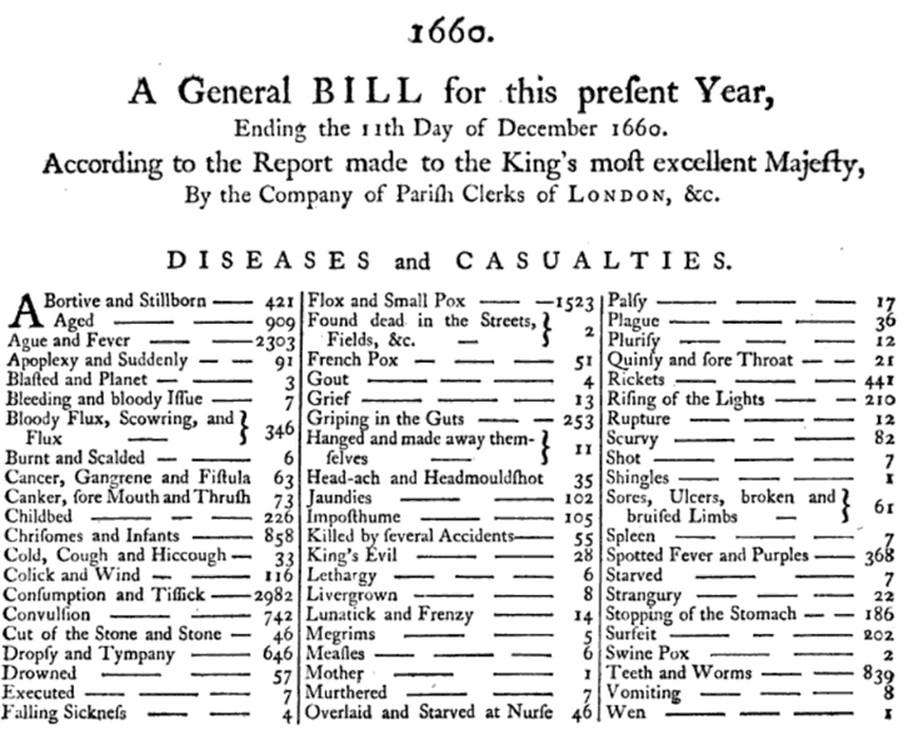
\includegraphics[width=1\linewidth]{images/StandardizedVocabularies/bill} 

}

\caption{1660 London Bill of Mortality, showing the cause of death for deceased inhabitants using a classification system of 62 diseases known at the time.}\label{fig:bill}
\end{figure}

Since then, the classifications have greatly expanded in size and
complexity and spread into other aspects of healthcare, such as
procedures and services, drugs, medical devices, etc. The main
principles have remained the same: they are controlled vocabularies,
terminologies, hierarchies or ontologies that some healthcare
communities agree upon for the purpose of capturing, classifying and
analyzing patient data. Many of these vocabularies are maintained by
public and government agencies with a long-term mandate for doing so.
For example, the World Health Organization (WHO) produces the
International Classification of Disease (ICD) with the recent addition
of its 11th revision (ICD11). Local governments create country-specific
versions, such as ICD10CM (USA), ICD10GM (Germany), etc. Governments
also control the marketing and sale of drugs and maintain national
repositories of such certified drugs. Vocabularies are also used in the
private sector, either as commercial products or for internal use, such
as electronic health record (EHR) systems or for medical insurance claim
reporting.

As a result, each country, region, healthcare system and institution
tends to have their own classifications that would most likely only be
relevant where it is used. This myriad of vocabularies prevents
interoperability of the systems they are used in. Standardization is the
key that enables patient data exchange, unlocks health data analysis on
a global level and allows systematic and standardized research,
including performance characterization and quality assessment. To
address that problem, multinational organizations have sprung up and
started creating broad standards, such as the WHO mentioned above and
the Standard Nomenclature of Medicine (SNOMED) or Logical Observation
Identifiers Names and Codes (LOINC). In the US, the Health IT Standards
Committee (HITAC) recommends the use of SNOMED, LOINC and the drug
vocabulary RxNorm as standards to the National Coordinator for Health IT
(ONC) for use in a common platform for nationwide health information
exchange across diverse entities.

OHDSI developed the OMOP CDM, a global standard for observational
research. As part of the CDM, the OMOP Standardized Vocabularies are
available for two main purposes:

\begin{itemize}
\tightlist
\item
  Common repository of all vocabularies used in the community
\item
  Standardization and mapping for use in research
\end{itemize}

The Standardized Vocabularies are available to the community free of
charge and \textbf{must be used} for OMOP CDM instance \textbf{as its
mandatory reference table}.

\subsection{Building the Standardized
Vocabularies}\label{building-the-standardized-vocabularies}

All vocabularies of the Standardized Vocabularies are consolidated into
the same common format. This relieves the researchers from having to
understand and handle multiple different formats and life-cycle
conventions of the originating vocabularies. All vocabularies are
regularly refreshed and incorporated using the Pallas system.\footnote{\url{https://github.com/OHDSI/Vocabulary-v5.0}}
It is built and run by the OHDSI Vocabulary Team, which is part of the
overall OMOP CDM Workgroup. If you find mistakes please report and help
improve our resource by posting in either the OHDSI Forums\footnote{\url{https://forums.ohdsi.org}}
or CDM Github page.\footnote{\url{https://github.com/OHDSI/CommonDataModel/issues}}
\index{Pallas system}

\subsection{Access to the Standardized
Vocabularies}\label{accessVocabularies}

In order to obtain the Standardized Vocabularies, you do not have to run
Pallas yourself. Instead, you can download the latest version from
ATHENA\footnote{\url{http://athena.ohdsi.org}} and load it into your
local database. ATHENA also allows faceted search of the Vocabularies.
\index{ATHENA} \index{standardized vocabularies!download}
\index{standardized vocabularies!search}

To download a zip file with all Standardized Vocabularies tables select
all the vocabularies you need for your OMOP CDM. Vocabularies with
Standard Concepts (see Section \ref{standardConcepts}) and very common
usage are preselected. Add vocabularies that are used in your source
data. Vocabularies that are proprietary have no select button. Click on
the ``License required'' button to incorporate such a vocabulary into
your list. The Vocabulary Team will contact you and request you
demonstrate your license or help you connect to the right folks to
obtain one.

\subsection{Source of Vocabularies: Adopt Versus
Build}\label{source-of-vocabularies-adopt-versus-build}

OHDSI generally prefers adopting existing vocabularies, rather than
de-novo construction, because (i) many vocabularies have already been
utilized in observational data in the community, and (ii) construction
and maintenance of vocabularies is complex and requires the input of
many stakeholders over long periods of time to mature. For that reason,
dedicated organizations provide vocabularies, which are subject to a
life-cycle of generation, deprecation, merging and splitting (see
Section \ref{conceptLifeCycle}). Currently, OHDSI only produces internal
administrative vocabularies like Type Concepts (e.g.~condition type
concepts). The only exception is RxNorm Extension, a vocabulary covering
drugs that are only used outside the United States (see Section
\ref{rxNormExtension}).

\section{Concepts}\label{concepts}

All clinical events in the OMOP CDM are expressed as concepts, which
represent the semantic notion of each event. They are the fundamental
building blocks of the data records, making almost all tables fully
normalized with few exceptions. Concepts are stored in the CONCEPT table
(see Figure \ref{fig:concept}). \index{concept}

\begin{figure}

{\centering 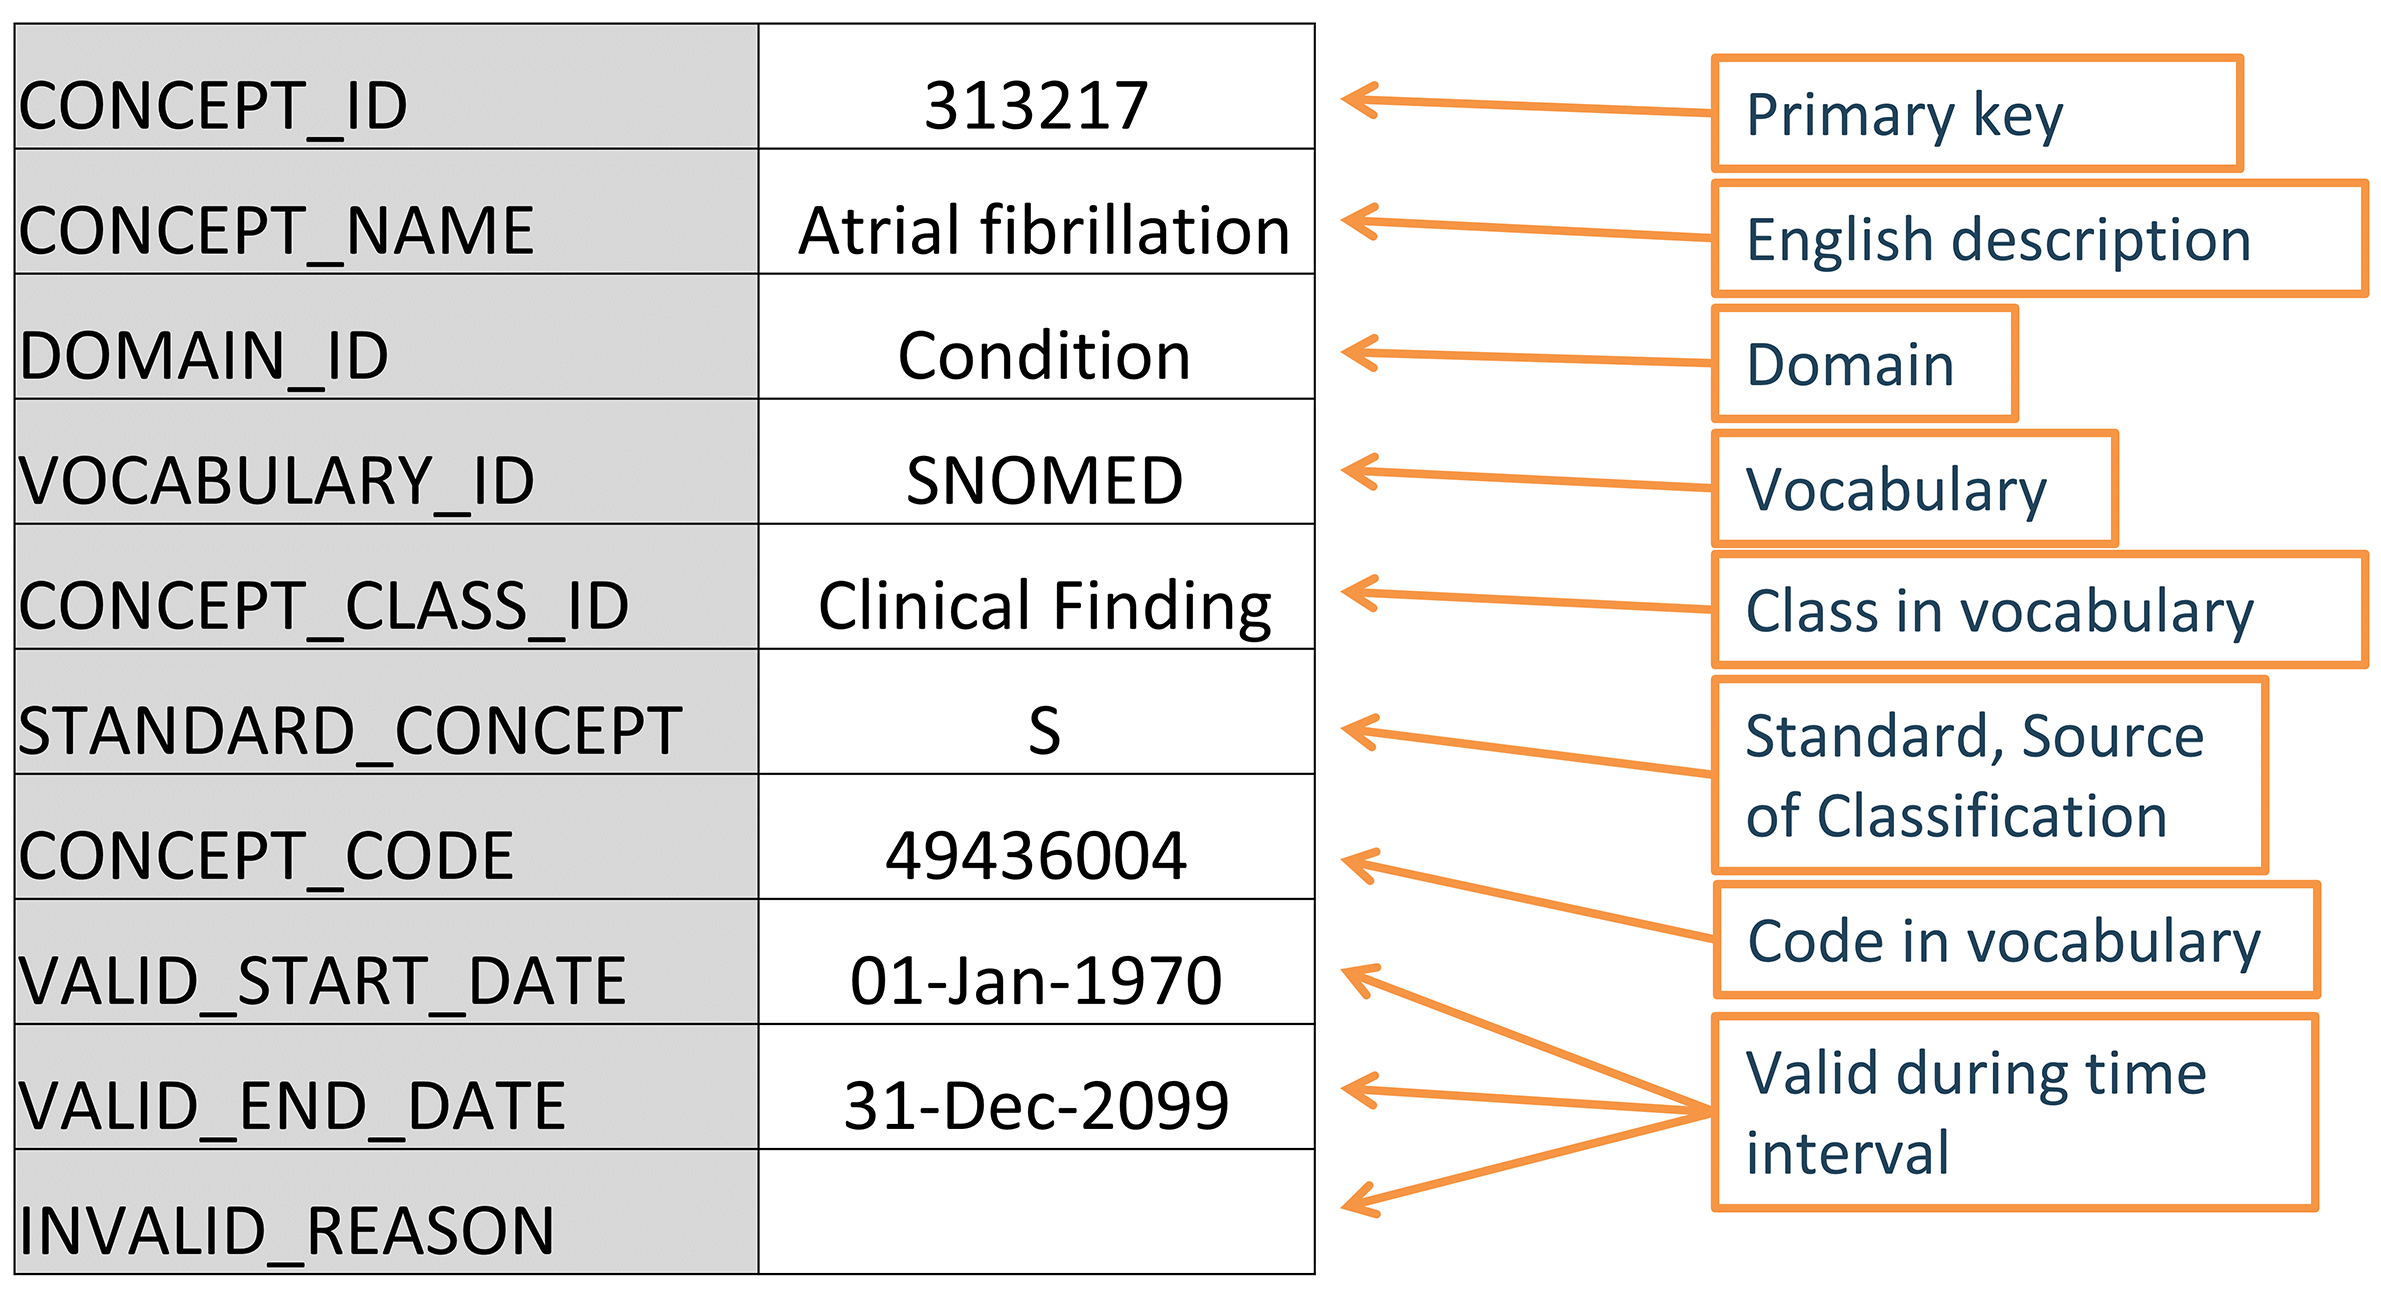
\includegraphics[width=0.9\linewidth]{images/StandardizedVocabularies/concept} 

}

\caption{Standard representation of vocabulary concepts in the OMOP CDM. The example provided is the CONCEPT table record for the SNOMED code for Atrial Fibrillation.}\label{fig:concept}
\end{figure}

This system is meant to be \textbf{comprehensive}, i.e.~there are enough
concepts to cover any event relevant to the patient's healthcare
experience (e.g.~conditions, procedures, exposures to drug, etc.) as
well as some of the administrative information of the healthcare system
(e.g.~visits, care sites, etc.).

\subsection{Concept IDs}\label{concept-ids}

Each concept is assigned a concept ID to be used as a primary key. This
meaningless integer ID, rather than the original code from the
vocabulary, is used to record data in the CDM event tables.
\index{concept!identifier}

\subsection{Concept Names}\label{concept-names}

Each concept has one name. Names are always in English. They are
imported from the source of the vocabulary. If the source vocabulary has
more than one name, the most expressive is selected and the remaining
ones are stored in the CONCEPT\_SYNONYM table under the same CONCEPT\_ID
key. Non-English names are recorded in CONCEPT\_SYNONYM as well, with
the appropriate language concept ID in the LANGUAGE\_CONCEPT\_ID field.
The name is 255 characters long, which means that very long names get
truncated and the full-length version recorded as another synonym, which
can hold up to 1000 characters.

\subsection{Domains}\label{conceptDomains}

Each concept is assigned a domain in the DOMAIN\_ID field, which in
contrast to the numerical CONCEPT\_ID is a short case-sensitive unique
alphanumeric ID for the domain. Examples of such domain identifiers are
``Condition,'' ``Drug,'' ``Procedure,'' ``Visit,'' ``Device,''
``Specimen,'' etc. Ambiguous or pre-coordinated (combination) concepts
can belong to a combination domain, but Standard Concepts (see Section
\ref{standardConcepts}) are always assigned a singular domain. Domains
also direct to which CDM table and field a clinical event or event
attribute is recorded. Domain assignments are an OMOP-specific feature
done during vocabulary ingestion using a heuristic laid out in
\href{https://github.com/ohDSI/vocabulary-v5.0}{Pallas}. Source
vocabularies tend to combine codes of mixed domains, but to a varying
degree (see Figure \ref{fig:domains}). \index{domain!concept}

\begin{figure}

{\centering 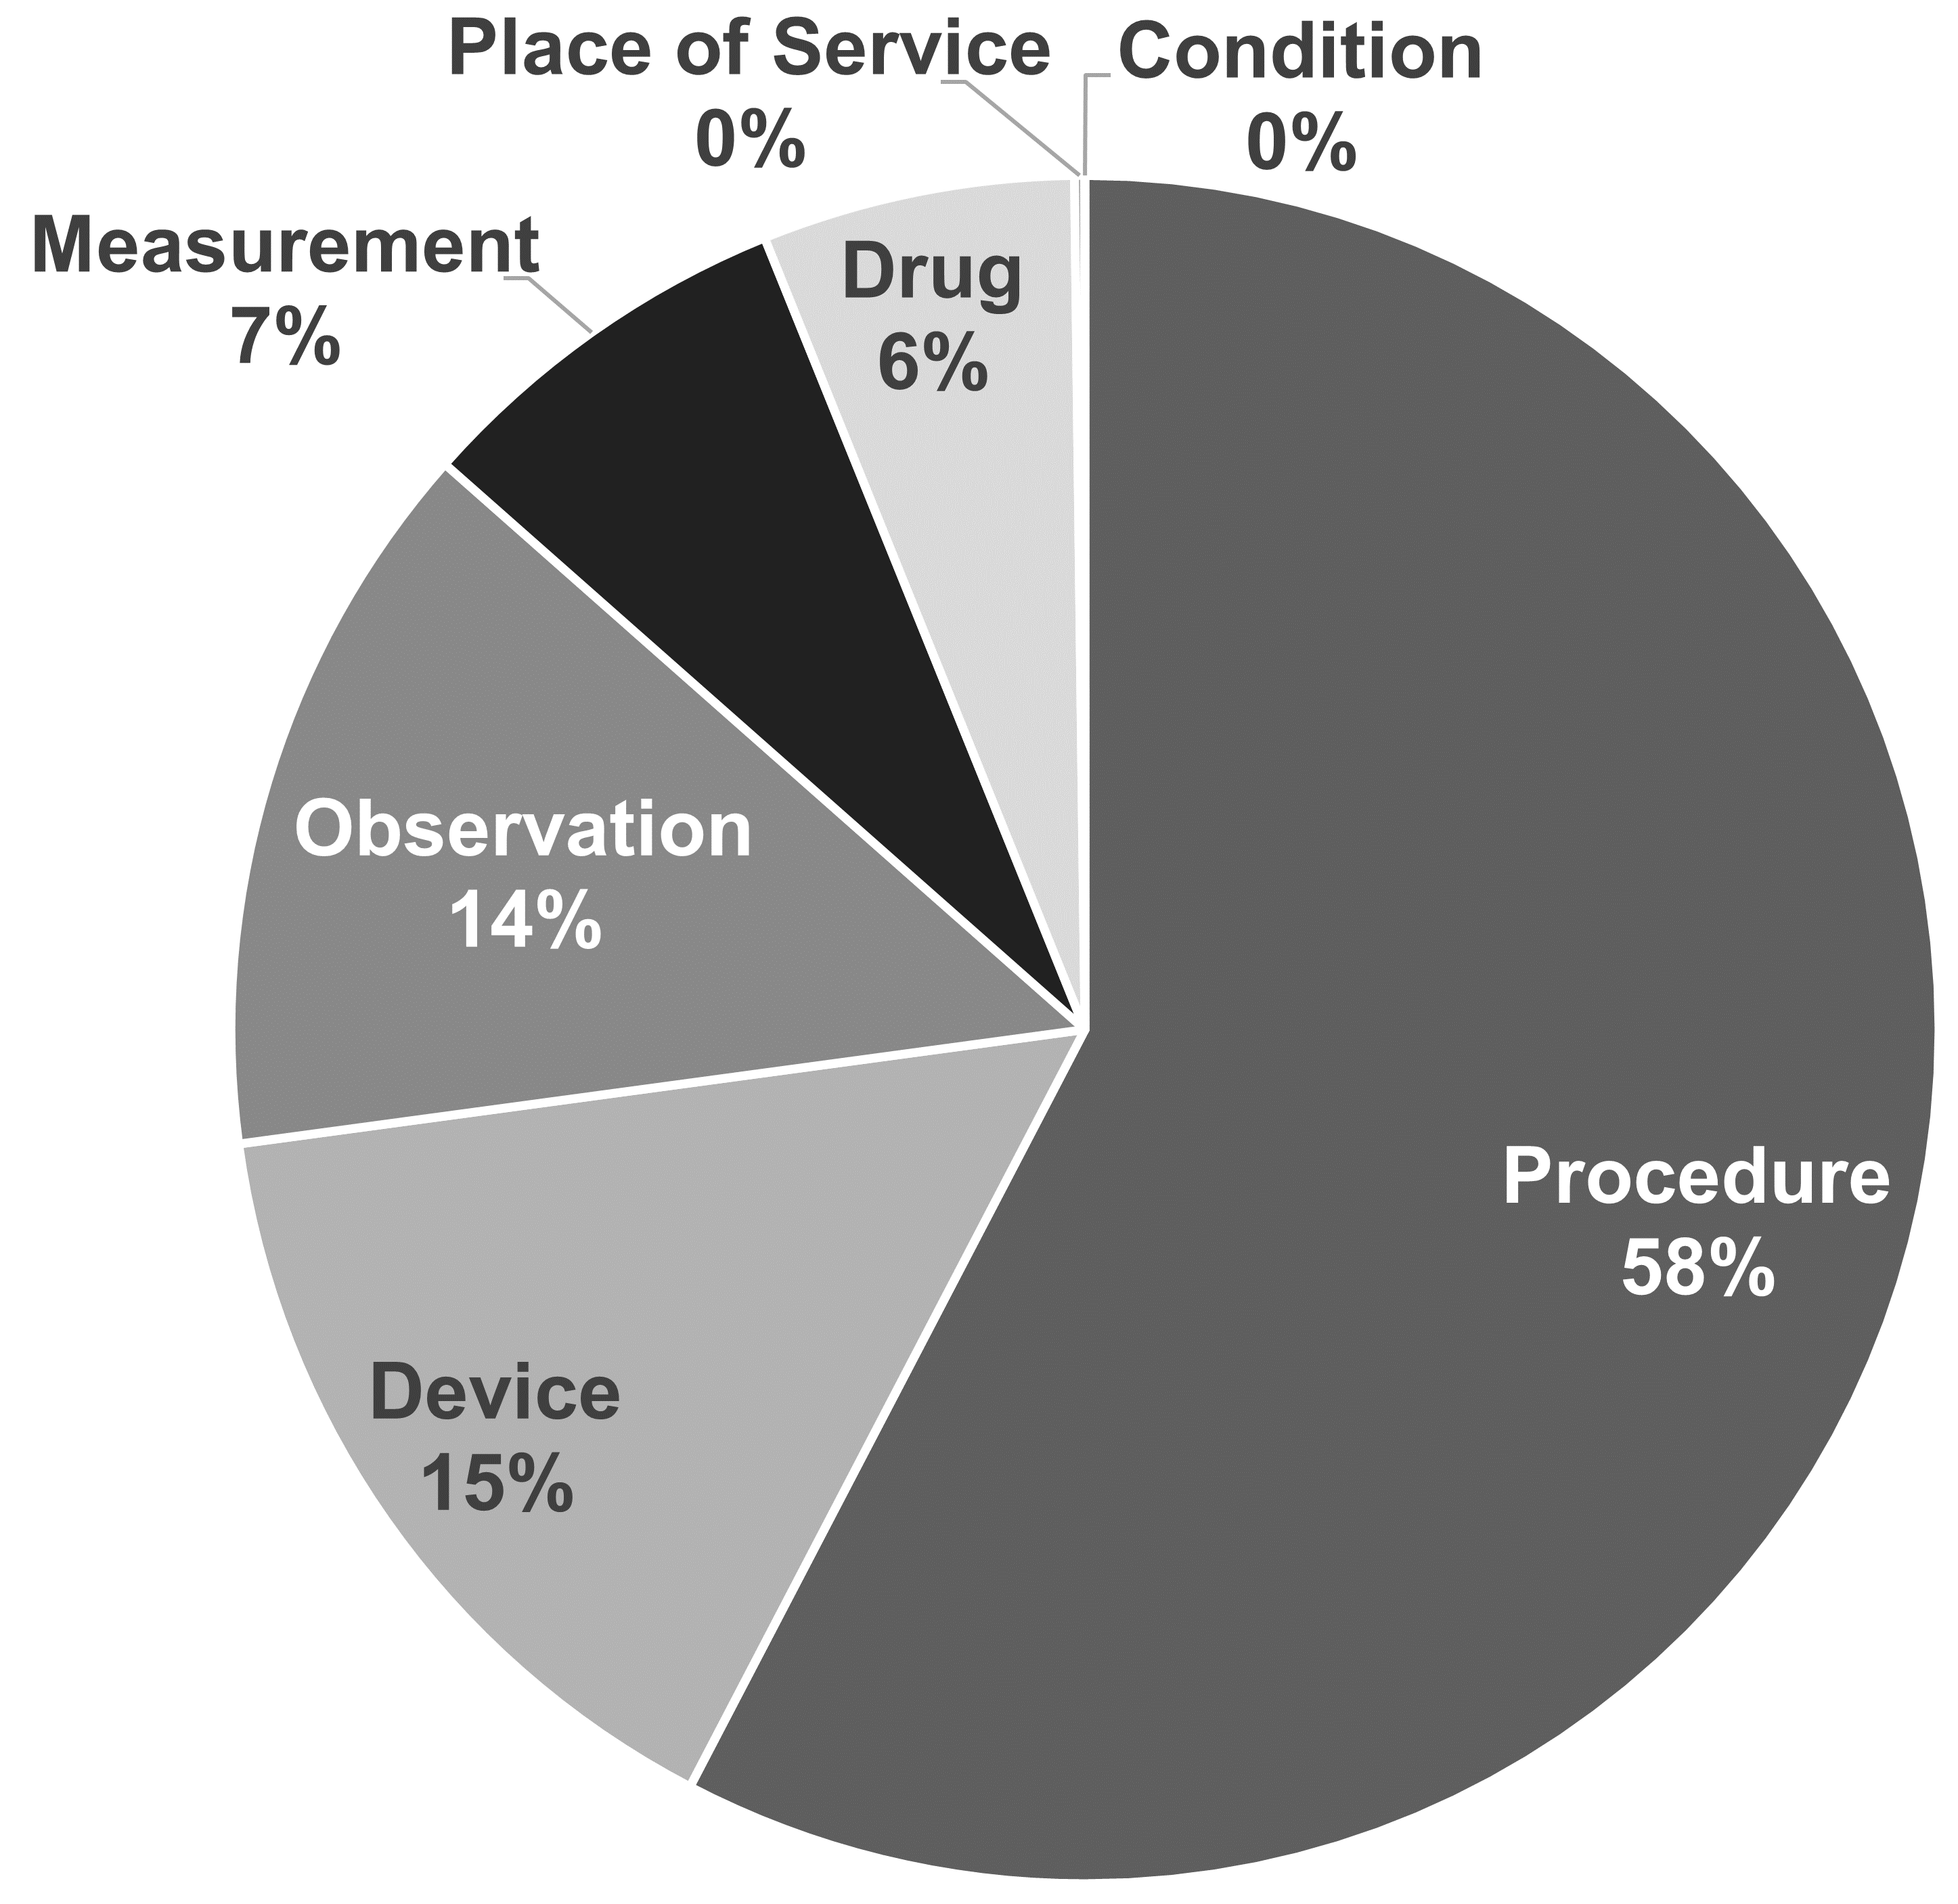
\includegraphics[width=0.7\linewidth]{images/StandardizedVocabularies/domains} 

}

\caption{Domain assignment in procedure vocabularies CPT4 and HCPCS. By intuition, these vocabularies should contain codes and concepts of a single domain, but in reality they are mixed.}\label{fig:domains}
\end{figure}

The domain heuristic follows the definitions of the domains. These
definitions are derived from the table and field definitions in the CDM
(see Chapter \ref{CommonDataModel}). The heuristic is not perfect; there
are grey zones (see Section \ref{specialSituations} ``Special
Situations''). If you find concept domains assigned incorrectly please
report and help improve the process through a
\href{https://forums.ohdsi.org}{Forums} or
\href{https://github.com/OHDSI/CommonDataModel/issues}{CDM issue} post.

\subsection{Vocabularies}\label{vocabularies}

Each vocabulary has a short case-sensitive unique alphanumeric ID, which
generally follows the abbreviated name of the vocabulary, omitting
dashes. For example, ICD-9-CM has the vocabulary ID ``ICD9CM''. There
are 111 vocabularies currently supported by OHDSI, of which 78 are
adopted from external sources, while the rest are OMOP-internal
vocabularies. These vocabularies are typically refreshed at a quarterly
schedule. The source and the version of the vocabularies is defined in
the VOCABULARY reference file. \index{vocabulary}

\subsection{Concept Classes}\label{concept-classes}

Some vocabularies classify their codes or concepts, denoted through
their case-sensitive unique alphanumerical IDs. For example, SNOMED has
33 such concept classes, which SNOMED refers to as ``semantic tags'':
clinical finding, social context, body structure, etc. These are
vertical divisions of the concepts. Others, such as MedDRA or RxNorm,
have concept classes classifying horizontal levels in their stratified
hierarchies. Vocabularies without any concept classes, such as HCPCS,
use the vocabulary ID as the Concept Class ID. \index{concept!class}

\begin{longtable}[]{@{}ll@{}}
\caption{\label{tab:sublassification} Vocabularies with or without
horizontal and vertical sub-classification principles in concept
class.}\tabularnewline
\toprule
\begin{minipage}[b]{0.13\columnwidth}\raggedright\strut
Concept class subdivision principle\strut
\end{minipage} & \begin{minipage}[b]{0.47\columnwidth}\raggedright\strut
Vocabulary\strut
\end{minipage}\tabularnewline
\midrule
\endfirsthead
\toprule
\begin{minipage}[b]{0.13\columnwidth}\raggedright\strut
Concept class subdivision principle\strut
\end{minipage} & \begin{minipage}[b]{0.47\columnwidth}\raggedright\strut
Vocabulary\strut
\end{minipage}\tabularnewline
\midrule
\endhead
\begin{minipage}[t]{0.13\columnwidth}\raggedright\strut
Horizontal\strut
\end{minipage} & \begin{minipage}[t]{0.47\columnwidth}\raggedright\strut
all drug vocabularies, ATC, CDТ, Episode, HCPCS, HemOnc, ICDs, MedDRA,
OSM, Census\strut
\end{minipage}\tabularnewline
\begin{minipage}[t]{0.13\columnwidth}\raggedright\strut
Vertical\strut
\end{minipage} & \begin{minipage}[t]{0.47\columnwidth}\raggedright\strut
CIEL, HES Specialty, ICDO3, MeSH, NAACCR, NDFRT, OPCS4, PCORNET, Plan,
PPI, Provider, SNOMED, SPL, UCUM\strut
\end{minipage}\tabularnewline
\begin{minipage}[t]{0.13\columnwidth}\raggedright\strut
Mixed\strut
\end{minipage} & \begin{minipage}[t]{0.47\columnwidth}\raggedright\strut
CPT4, ISBT, LOINC\strut
\end{minipage}\tabularnewline
\begin{minipage}[t]{0.13\columnwidth}\raggedright\strut
None\strut
\end{minipage} & \begin{minipage}[t]{0.47\columnwidth}\raggedright\strut
APC, all Type Concepts, Ethnicity, OXMIS, Race, Revenue Code, Sponsor,
Supplier, UB04s, Visit\strut
\end{minipage}\tabularnewline
\bottomrule
\end{longtable}

Horizontal concept classes allow you to determine a specific
hierarchical level. For example, in the drug vocabulary RxNorm the
concept class ``Ingredient'' defines the top level of the hierarchy. In
the vertical model, members of a concept class can be of any
hierarchical level from the top to the very bottom.

\subsection{Standard Concepts}\label{standardConcepts}

One concept representing the meaning of each clinical event is
designated the Standard. For example, MESH code D001281, CIEL code
148203, SNOMED code 49436004, ICD9CM code 427.31 and Read code G573000
all define ``Atrial fibrillation'' in the condition domain, but only the
SNOMED concept is Standard and represents the condition in the data. The
others are designated non-standard or source concepts and mapped to the
Standard ones. Standard Concepts are indicated through an ``S'' in the
STANDARD\_CONCEPT field. And only these Standard Concepts are used to
record data in the CDM fields ending in ``\_CONCEPT\_ID``.
\index{standard concept}

\subsection{Non-Standard Concepts}\label{non-standard-concepts}

Non-standard concepts are not used to represent the clinical events, but
they are still part of the Standardized Vocabularies, and are often
found in the source data. For that reason, they are also called ``source
concepts''. The conversion of source concepts to Standard Concepts is a
process called ``mapping'' (see Section \ref{conceptMapping}).
Non-standard concepts have no value (NULL) In the STANDARD\_CONCEPT
field.

\subsection{Classification Concepts}\label{classification-concepts}

These concepts are not Standard, and hence cannot be used to represent
the data. But they are participating in the hierarchy with the Standard
Concepts, and can therefore be used to perform hierarchical queries. For
example, querying for all descendants of MedDRA code 10037908 (not
visible for users who have not obtained a MedDRA license, see Section
\ref{accessVocabularies} for access restrictions) will retrieve the
Standard SNOMED concept for Atrial Fibrillation (see Section
\ref{conceptAncestor} for hierarchical queries using the
CONCEPT\_ANCESTOR table) - see Figure \ref{fig:hierarchy}.
\index{classification concept}

\begin{figure}

{\centering 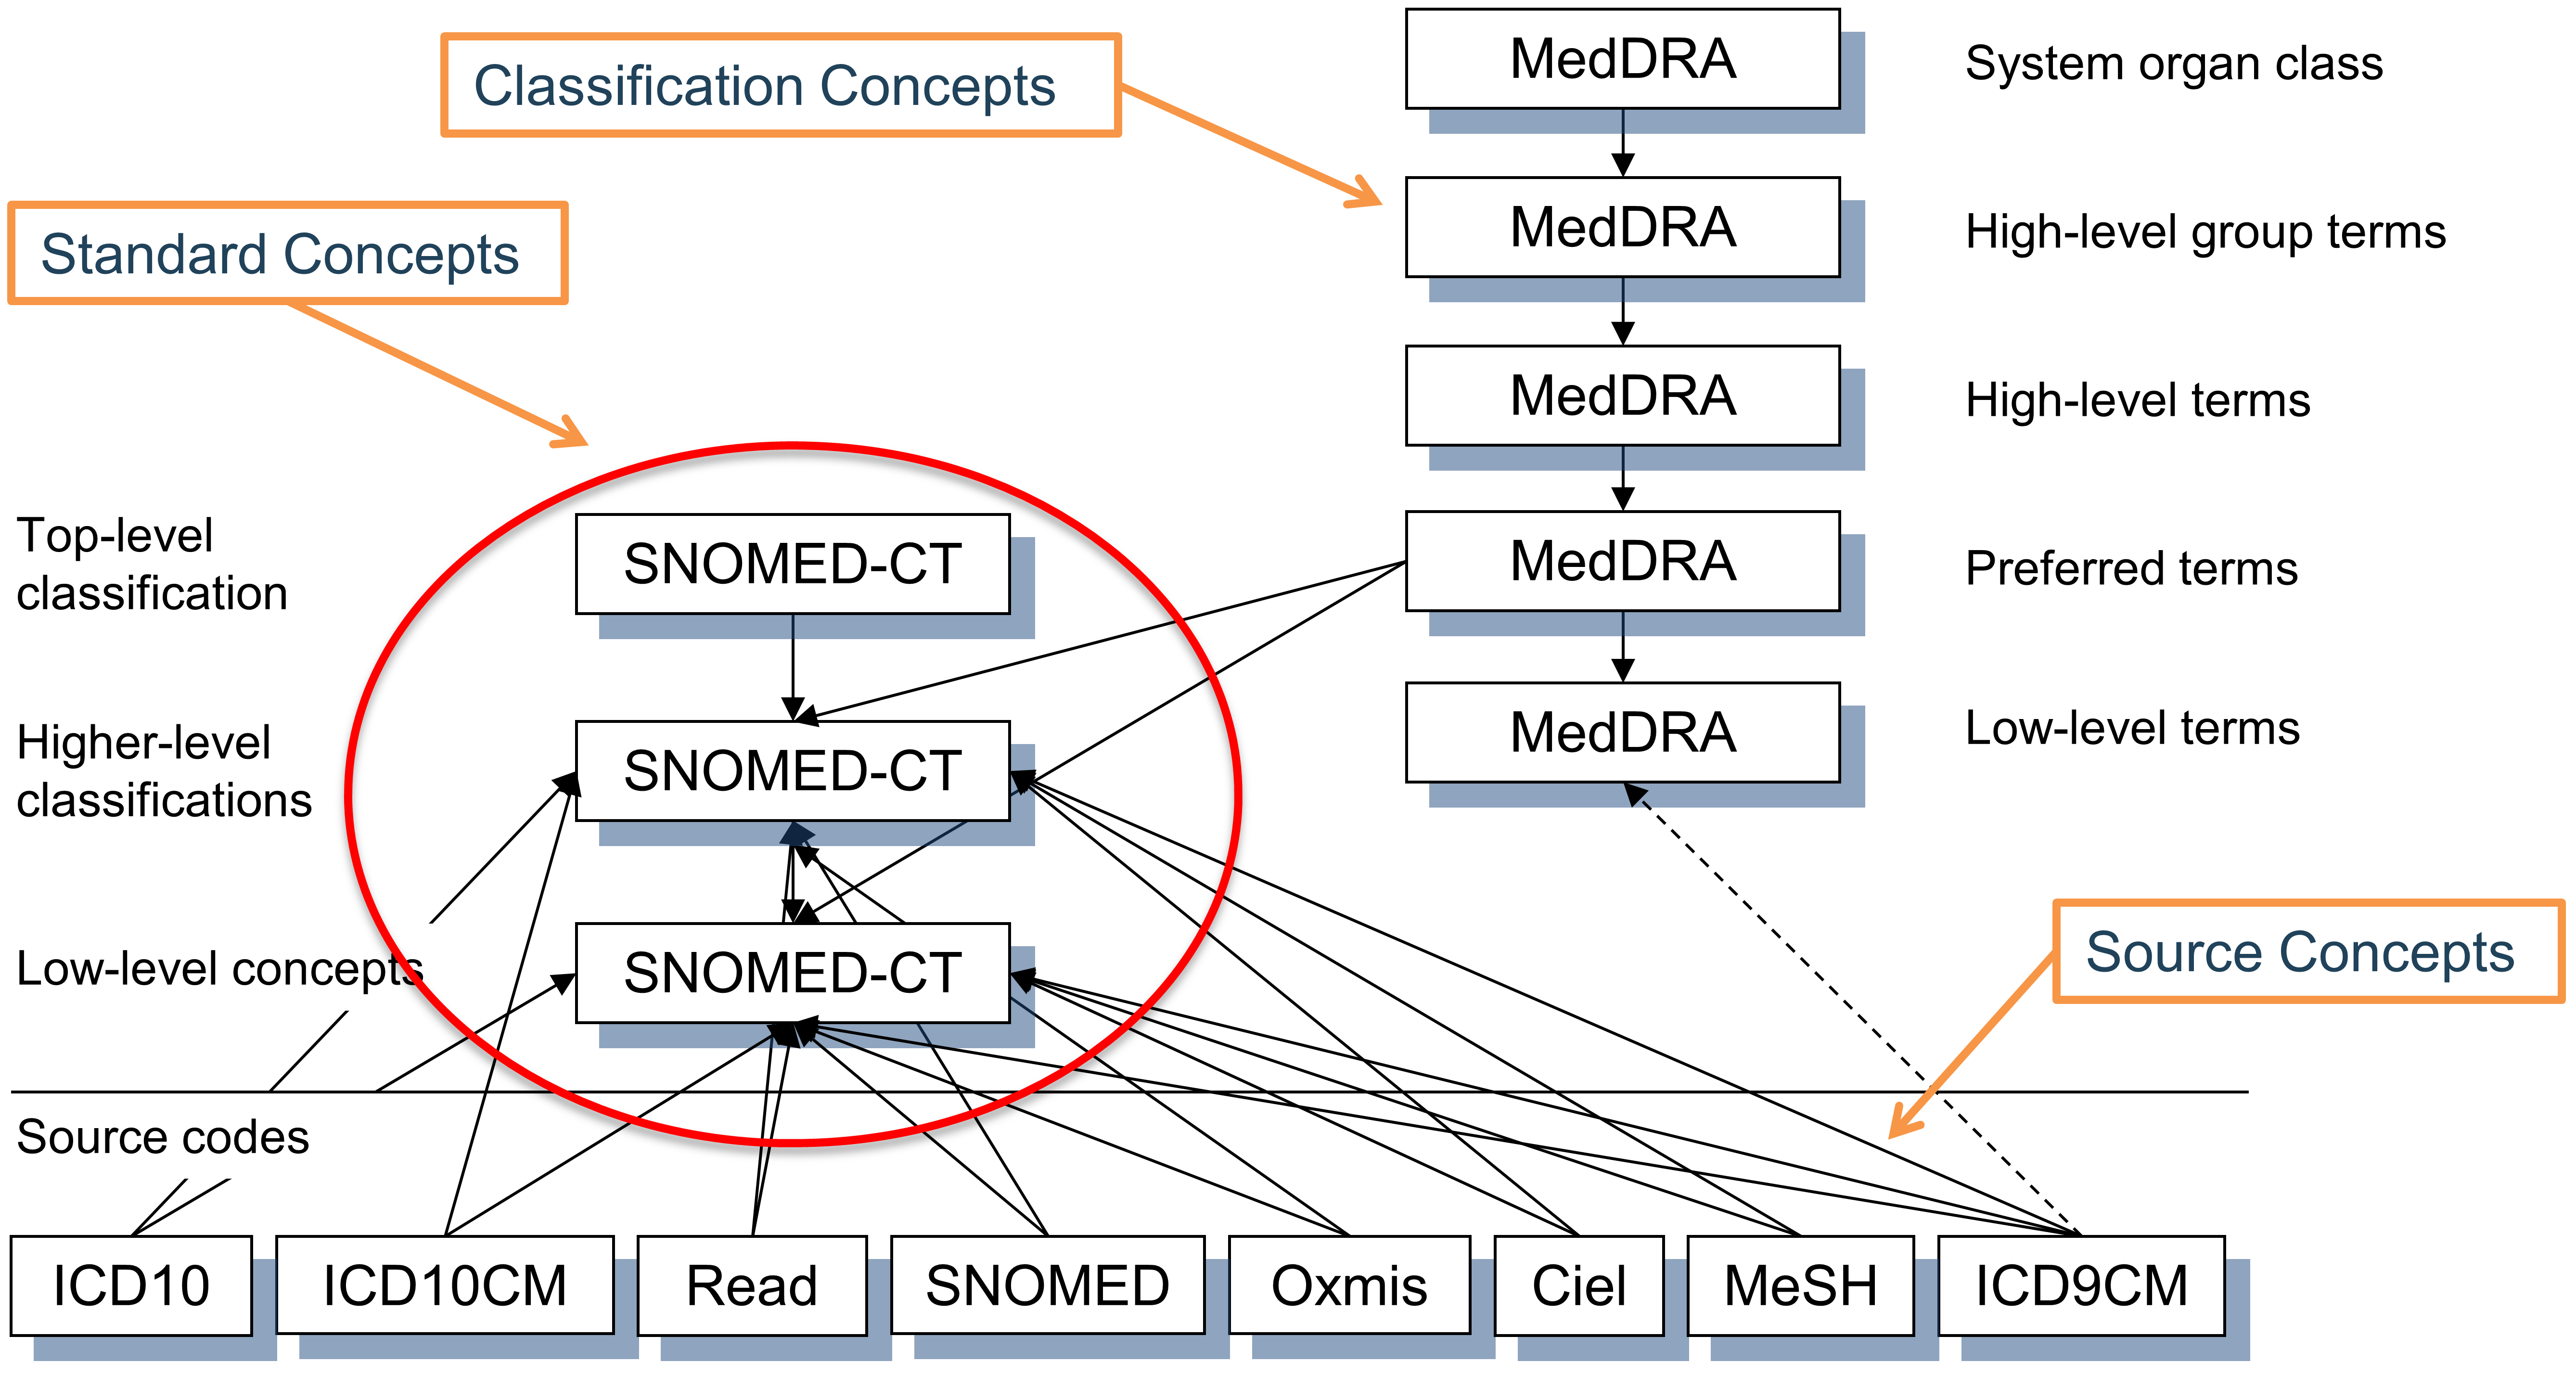
\includegraphics[width=1\linewidth]{images/StandardizedVocabularies/hierarchy} 

}

\caption{Standard, non-standard source and classification concepts and their hierarchical relationships in the condition domain. SNOMED is used for most standard condition concepts (with some oncology-related concepts derived from ICDO3), MedDRA concepts are used for hierarchical classification concepts, and all other vocabularies contain non-standard or source concepts, which do not participate in the hierarchy.}\label{fig:hierarchy}
\end{figure}

The choice of concept designation as Standard, non-standard and
classification is typically done for each domain separately at the
vocabulary level. This is based on the quality of the concepts, the
built-in hierarchy and the declared purpose of the vocabulary. Also, not
all concepts of a vocabulary are used as Standard Concepts. The
designation is separate for each domain, each concept has to be active
(see Section \ref{conceptLifeCycle}) and there might be an order of
precedence if more than one concept from different vocabularies compete
for the same meaning. In other words, there is no such a thing as a
``standard vocabulary.'' See Table \ref{tab:vocabList} for examples.

\begin{longtable}[]{@{}llll@{}}
\caption{\label{tab:vocabList} List of vocabularies to utilize for
Standard/non-standard/classification concept
assignments.}\tabularnewline
\toprule
\begin{minipage}[b]{0.12\columnwidth}\raggedright\strut
Domain\strut
\end{minipage} & \begin{minipage}[b]{0.21\columnwidth}\raggedright\strut
for Standard Concepts\strut
\end{minipage} & \begin{minipage}[b]{0.21\columnwidth}\raggedright\strut
for source concepts\strut
\end{minipage} & \begin{minipage}[b]{0.18\columnwidth}\raggedright\strut
for classification concepts\strut
\end{minipage}\tabularnewline
\midrule
\endfirsthead
\toprule
\begin{minipage}[b]{0.12\columnwidth}\raggedright\strut
Domain\strut
\end{minipage} & \begin{minipage}[b]{0.21\columnwidth}\raggedright\strut
for Standard Concepts\strut
\end{minipage} & \begin{minipage}[b]{0.21\columnwidth}\raggedright\strut
for source concepts\strut
\end{minipage} & \begin{minipage}[b]{0.18\columnwidth}\raggedright\strut
for classification concepts\strut
\end{minipage}\tabularnewline
\midrule
\endhead
\begin{minipage}[t]{0.12\columnwidth}\raggedright\strut
Condition\strut
\end{minipage} & \begin{minipage}[t]{0.21\columnwidth}\raggedright\strut
SNOMED, ICDO3\strut
\end{minipage} & \begin{minipage}[t]{0.21\columnwidth}\raggedright\strut
SNOMED Veterinary\strut
\end{minipage} & \begin{minipage}[t]{0.18\columnwidth}\raggedright\strut
MedDRA\strut
\end{minipage}\tabularnewline
\begin{minipage}[t]{0.12\columnwidth}\raggedright\strut
Procedure\strut
\end{minipage} & \begin{minipage}[t]{0.21\columnwidth}\raggedright\strut
SNOMED, CPT4, HCPCS, ICD10PCS, ICD9Proc, OPCS4\strut
\end{minipage} & \begin{minipage}[t]{0.21\columnwidth}\raggedright\strut
SNOMED Veterinary, HemOnc, NAACCR\strut
\end{minipage} & \begin{minipage}[t]{0.18\columnwidth}\raggedright\strut
None at this point\strut
\end{minipage}\tabularnewline
\begin{minipage}[t]{0.12\columnwidth}\raggedright\strut
Measurement\strut
\end{minipage} & \begin{minipage}[t]{0.21\columnwidth}\raggedright\strut
SNOMED, LOINC\strut
\end{minipage} & \begin{minipage}[t]{0.21\columnwidth}\raggedright\strut
SNOMED Veterinary, NAACCR, CPT4, HCPCS, OPCS4, PPI\strut
\end{minipage} & \begin{minipage}[t]{0.18\columnwidth}\raggedright\strut
None at this point\strut
\end{minipage}\tabularnewline
\begin{minipage}[t]{0.12\columnwidth}\raggedright\strut
Drug\strut
\end{minipage} & \begin{minipage}[t]{0.21\columnwidth}\raggedright\strut
RxNorm, RxNorm Extension, CVX\strut
\end{minipage} & \begin{minipage}[t]{0.21\columnwidth}\raggedright\strut
HCPCS, CPT4, HemOnc, NAAACCR\strut
\end{minipage} & \begin{minipage}[t]{0.18\columnwidth}\raggedright\strut
ATC\strut
\end{minipage}\tabularnewline
\begin{minipage}[t]{0.12\columnwidth}\raggedright\strut
Device\strut
\end{minipage} & \begin{minipage}[t]{0.21\columnwidth}\raggedright\strut
SNOMED\strut
\end{minipage} & \begin{minipage}[t]{0.21\columnwidth}\raggedright\strut
Others, currently not normalized\strut
\end{minipage} & \begin{minipage}[t]{0.18\columnwidth}\raggedright\strut
None at this point\strut
\end{minipage}\tabularnewline
\begin{minipage}[t]{0.12\columnwidth}\raggedright\strut
Observation\strut
\end{minipage} & \begin{minipage}[t]{0.21\columnwidth}\raggedright\strut
SNOMED\strut
\end{minipage} & \begin{minipage}[t]{0.21\columnwidth}\raggedright\strut
Others\strut
\end{minipage} & \begin{minipage}[t]{0.18\columnwidth}\raggedright\strut
None at this point\strut
\end{minipage}\tabularnewline
\begin{minipage}[t]{0.12\columnwidth}\raggedright\strut
Visit\strut
\end{minipage} & \begin{minipage}[t]{0.21\columnwidth}\raggedright\strut
CMS Place of Service, ABMT, NUCC\strut
\end{minipage} & \begin{minipage}[t]{0.21\columnwidth}\raggedright\strut
SNOMED, HCPCS, CPT4, UB04\strut
\end{minipage} & \begin{minipage}[t]{0.18\columnwidth}\raggedright\strut
None at this point\strut
\end{minipage}\tabularnewline
\bottomrule
\end{longtable}

\subsection{Concept Codes}\label{concept-codes}

Concept codes are the identifiers used in the source vocabularies. For
example, ICD9CM or NDC codes are stored in this field, while the OMOP
tables use the concept ID as a foreign key into the CONCEPT table. The
reason is that the name space overlaps across vocabularies, i.e.~the
same code can exist in different vocabularies with completely different
meanings (see Table \ref{tab:code1001}) \index{concept!code}

\begin{longtable}[]{@{}llllll@{}}
\caption{\label{tab:code1001} Concepts with identical concept code 1001, but
different vocabularies, domains and concept classes.}\tabularnewline
\toprule
\begin{minipage}[b]{0.13\columnwidth}\raggedright\strut
Concept ID\strut
\end{minipage} & \begin{minipage}[b]{0.07\columnwidth}\raggedright\strut
Concept Code\strut
\end{minipage} & \begin{minipage}[b]{0.16\columnwidth}\raggedright\strut
Concept Name\strut
\end{minipage} & \begin{minipage}[b]{0.14\columnwidth}\raggedright\strut
Domain ID\strut
\end{minipage} & \begin{minipage}[b]{0.14\columnwidth}\raggedright\strut
Vocabulary ID\strut
\end{minipage} & \begin{minipage}[b]{0.14\columnwidth}\raggedright\strut
Concept Class\strut
\end{minipage}\tabularnewline
\midrule
\endfirsthead
\toprule
\begin{minipage}[b]{0.13\columnwidth}\raggedright\strut
Concept ID\strut
\end{minipage} & \begin{minipage}[b]{0.07\columnwidth}\raggedright\strut
Concept Code\strut
\end{minipage} & \begin{minipage}[b]{0.16\columnwidth}\raggedright\strut
Concept Name\strut
\end{minipage} & \begin{minipage}[b]{0.14\columnwidth}\raggedright\strut
Domain ID\strut
\end{minipage} & \begin{minipage}[b]{0.14\columnwidth}\raggedright\strut
Vocabulary ID\strut
\end{minipage} & \begin{minipage}[b]{0.14\columnwidth}\raggedright\strut
Concept Class\strut
\end{minipage}\tabularnewline
\midrule
\endhead
\begin{minipage}[t]{0.13\columnwidth}\raggedright\strut
35803438\strut
\end{minipage} & \begin{minipage}[t]{0.07\columnwidth}\raggedright\strut
1001\strut
\end{minipage} & \begin{minipage}[t]{0.16\columnwidth}\raggedright\strut
Granulocyte colony-stimulating factors\strut
\end{minipage} & \begin{minipage}[t]{0.14\columnwidth}\raggedright\strut
Drug\strut
\end{minipage} & \begin{minipage}[t]{0.14\columnwidth}\raggedright\strut
HemOnc\strut
\end{minipage} & \begin{minipage}[t]{0.14\columnwidth}\raggedright\strut
Component Class\strut
\end{minipage}\tabularnewline
\begin{minipage}[t]{0.13\columnwidth}\raggedright\strut
35942070\strut
\end{minipage} & \begin{minipage}[t]{0.07\columnwidth}\raggedright\strut
1001\strut
\end{minipage} & \begin{minipage}[t]{0.16\columnwidth}\raggedright\strut
AJCC TNM Clin T\strut
\end{minipage} & \begin{minipage}[t]{0.14\columnwidth}\raggedright\strut
Measurement\strut
\end{minipage} & \begin{minipage}[t]{0.14\columnwidth}\raggedright\strut
NAACCR\strut
\end{minipage} & \begin{minipage}[t]{0.14\columnwidth}\raggedright\strut
NAACCR Variable\strut
\end{minipage}\tabularnewline
\begin{minipage}[t]{0.13\columnwidth}\raggedright\strut
1036059\strut
\end{minipage} & \begin{minipage}[t]{0.07\columnwidth}\raggedright\strut
1001\strut
\end{minipage} & \begin{minipage}[t]{0.16\columnwidth}\raggedright\strut
Antipyrine\strut
\end{minipage} & \begin{minipage}[t]{0.14\columnwidth}\raggedright\strut
Drug\strut
\end{minipage} & \begin{minipage}[t]{0.14\columnwidth}\raggedright\strut
RxNorm\strut
\end{minipage} & \begin{minipage}[t]{0.14\columnwidth}\raggedright\strut
Ingredient\strut
\end{minipage}\tabularnewline
\begin{minipage}[t]{0.13\columnwidth}\raggedright\strut
38003544\strut
\end{minipage} & \begin{minipage}[t]{0.07\columnwidth}\raggedright\strut
1001\strut
\end{minipage} & \begin{minipage}[t]{0.16\columnwidth}\raggedright\strut
Residential Treatment - Psychiatric\strut
\end{minipage} & \begin{minipage}[t]{0.14\columnwidth}\raggedright\strut
Revenue Code\strut
\end{minipage} & \begin{minipage}[t]{0.14\columnwidth}\raggedright\strut
Revenue Code\strut
\end{minipage} & \begin{minipage}[t]{0.14\columnwidth}\raggedright\strut
Revenue Code\strut
\end{minipage}\tabularnewline
\begin{minipage}[t]{0.13\columnwidth}\raggedright\strut
43228317\strut
\end{minipage} & \begin{minipage}[t]{0.07\columnwidth}\raggedright\strut
1001\strut
\end{minipage} & \begin{minipage}[t]{0.16\columnwidth}\raggedright\strut
Aceprometazine maleate\strut
\end{minipage} & \begin{minipage}[t]{0.14\columnwidth}\raggedright\strut
Drug\strut
\end{minipage} & \begin{minipage}[t]{0.14\columnwidth}\raggedright\strut
BDPM\strut
\end{minipage} & \begin{minipage}[t]{0.14\columnwidth}\raggedright\strut
Ingredient\strut
\end{minipage}\tabularnewline
\begin{minipage}[t]{0.13\columnwidth}\raggedright\strut
45417187\strut
\end{minipage} & \begin{minipage}[t]{0.07\columnwidth}\raggedright\strut
1001\strut
\end{minipage} & \begin{minipage}[t]{0.16\columnwidth}\raggedright\strut
Brompheniramine Maleate, 10 mg/mL injectable solution\strut
\end{minipage} & \begin{minipage}[t]{0.14\columnwidth}\raggedright\strut
Drug\strut
\end{minipage} & \begin{minipage}[t]{0.14\columnwidth}\raggedright\strut
Multum\strut
\end{minipage} & \begin{minipage}[t]{0.14\columnwidth}\raggedright\strut
Multum\strut
\end{minipage}\tabularnewline
\begin{minipage}[t]{0.13\columnwidth}\raggedright\strut
45912144\strut
\end{minipage} & \begin{minipage}[t]{0.07\columnwidth}\raggedright\strut
1001\strut
\end{minipage} & \begin{minipage}[t]{0.16\columnwidth}\raggedright\strut
Serum\strut
\end{minipage} & \begin{minipage}[t]{0.14\columnwidth}\raggedright\strut
Specimen\strut
\end{minipage} & \begin{minipage}[t]{0.14\columnwidth}\raggedright\strut
CIEL\strut
\end{minipage} & \begin{minipage}[t]{0.14\columnwidth}\raggedright\strut
Specimen\strut
\end{minipage}\tabularnewline
\bottomrule
\end{longtable}

\subsection{Life-Cycle}\label{conceptLifeCycle}

Vocabularies are rarely permanent corpora with a fixed set of codes.
Instead, codes and concepts are added and get deprecated. The OMOP CDM
is a model to support longitudinal patient data, which means it needs to
support concepts that were used in the past and might no longer be
active, as well as supporting new concepts and placing them into
context. There are three fields in the CONCEPT table that describe the
possible life-cycle statuses: VALID\_START\_DATE, VALID\_END\_DATE, and
INVALID\_REASON. Their values differ depending on the concept life-cycle
status:

\begin{itemize}
\tightlist
\item
  \textbf{Active or new concept}

  \begin{itemize}
  \tightlist
  \item
    Description: Concept in use.
  \item
    VALID\_START\_DATE: Day of instantiation of concept, if that is not
    known day of incorporation of concept in Vocabularies, if that is
    not known 1970-1-1.
  \item
    VALID\_END\_DATE: Set to 2099-12-31 as a convention to indicate
    ``Might become invalid in an undefined future, but active right
    now''.
  \item
    INVALID\_REASON: NULL
  \end{itemize}
\item
  \textbf{Deprecated Concept with no successor}

  \begin{itemize}
  \tightlist
  \item
    Description: Concept inactive and cannot be used as Standard (see
    Section \ref{standardConcepts}).
  \item
    VALID\_START\_DATE: Day of instantiation of concept, if that is not
    known day of incorporation of concept in Vocabularies, if that is
    not known 1970-1-1.
  \item
    VALID\_END\_DATE: Day in the past indicating deprecation, or if that
    is not known day of vocabulary refresh where concept in vocabulary
    went missing or set to inactive.
  \item
    INVALID\_REASON: ``D''
  \end{itemize}
\item
  \textbf{Upgraded Concept with successor}

  \begin{itemize}
  \tightlist
  \item
    Description: Concept inactive, but has defined successor. These are
    typically concepts which went through de-duplication.
  \item
    VALID\_START\_DATE: Day of instantiation of concept, if that is not
    known day of incorporation of concept in Vocabularies, if that is
    not known 1970-1-1.
  \item
    VALID\_END\_DATE: Day in the past indicating an upgrade, or if that
    is not known day of vocabulary refresh where the upgrade was
    included.
  \item
    INVALID\_REASON: ``U''
  \end{itemize}
\item
  \textbf{Reused code for another new concept}

  \begin{itemize}
  \tightlist
  \item
    Description: The vocabulary reused the concept code of this
    deprecated concept for a new concept.
  \item
    VALID\_START\_DATE: Day of instantiation of concept, if that is not
    known day of incorporation of concept in Vocabularies, if that is
    not known 1970-1-1.
  \item
    VALID\_END\_DATE: Day in the past indicating deprecation, or if that
    is not known day of vocabulary refresh where concept in vocabulary
    went missing or set to inactive.
  \item
    INVALID\_REASON: ``R''
  \end{itemize}
\end{itemize}

In general, concept codes are not reused. But there are a few
vocabularies that deviate from this rule, in particular HCPCS, NDC and
DRG. For those, the same concept code appears in more than one concept
of the same vocabulary. Their CONCEPT\_ID value stays unique. These
reused concept codes are marked with an ``R'' in the INVALID\_REASON
field, and the VALID\_START\_DATE to VALID\_END\_DATE period should be
used to distinguish concepts with the same concept codes.

\section{Relationships}\label{relationships}

Any two concepts can have a defined relationship, regardless of whether
the two concepts belong to the same domain or vocabulary. The nature of
the relationships is indicated in its short case-sensitive unique
alphanumeric ID in the RELATIONSHIP\_ID field of the
CONCEPT\_RELATIONSHIP table. Relationships are symmetrical, i.e.~for
each relationship an equivalent relationship exists, where the content
of the fields CONCEPT\_ID\_1 and CONCEPT\_ID\_2 are swapped, and the
RELATIONHSIP\_ID is changed to its opposite. For example, the ``Maps
to'' relationship has an opposite relationship ``Mapped from.''
\index{concept!relationship}

CONCEPT\_RELATIONSHIP table records also have life-cycle fields
RELATIONSHIP\_START\_DATE, RELATIONSHIP\_END\_DATE and INVALID\_REASON.
However, only active records with INVALID\_REASON = NULL are available
through ATHENA. Inactive relationships are kept in the Pallas system for
internal processing only. The RELATIONSHIP table serves as the reference
with the full list of relationship IDs and their reverse counterparts.

\subsection{Mapping Relationships}\label{conceptMapping}

These relationships provide translations from non-standard to Standard
concepts, supported by two relationship ID pairs (see Table
\ref{tab:mappingRelationships}). \index{concept!mapping}

\begin{longtable}[]{@{}ll@{}}
\caption{\label{tab:mappingRelationships} Type of mapping
relationships.}\tabularnewline
\toprule
\begin{minipage}[b]{0.20\columnwidth}\raggedright\strut
Relationship ID pair\strut
\end{minipage} & \begin{minipage}[b]{0.71\columnwidth}\raggedright\strut
Purpose\strut
\end{minipage}\tabularnewline
\midrule
\endfirsthead
\toprule
\begin{minipage}[b]{0.20\columnwidth}\raggedright\strut
Relationship ID pair\strut
\end{minipage} & \begin{minipage}[b]{0.71\columnwidth}\raggedright\strut
Purpose\strut
\end{minipage}\tabularnewline
\midrule
\endhead
\begin{minipage}[t]{0.20\columnwidth}\raggedright\strut
``Maps to'' and ``Mapped from''\strut
\end{minipage} & \begin{minipage}[t]{0.71\columnwidth}\raggedright\strut
Mapping to Standard Concepts. Standard Concepts are mapped to
themselves, non-standard concepts to Standard Concepts. Most
non-standard and all Standard Concepts have this relationship to a
Standard Concept. The former are stored in *\_SOURCE\_CONCEPT\_ID, and
the latter in the *\_CONCEPT\_ID fields. Classification concepts are not
mapped.\strut
\end{minipage}\tabularnewline
\begin{minipage}[t]{0.20\columnwidth}\raggedright\strut
``Maps to value'' and ``Value mapped from''\strut
\end{minipage} & \begin{minipage}[t]{0.71\columnwidth}\raggedright\strut
Mapping to a concept that represents a Value to be placed into the
VALUE\_AS\_CONCEPT\_ID fields of the MEASUREMENT and OBSERVATION
tables.\strut
\end{minipage}\tabularnewline
\bottomrule
\end{longtable}

The purpose of these mapping relationships is to allow a crosswalk
between equivalent concepts to harmonize how clinical events are
represented in the OMOP CDM. This is a main achievement of the
Standardized Vocabularies.

``Equivalent concepts'' means it carries the same meaning, and,
importantly, the hierarchical descendants cover the same semantic space.
If an equivalent concept is not available and the concept is not
Standard, it is still mapped, but to a slightly broader concept
(so-called ``up-hill mappings''). For example, ICD10CM W61.51 ``Bitten
by goose'' has no equivalent in the SNOMED vocabulary, which is
generally used for standard condition concepts. Instead, it is mapped to
SNOMED 217716004 ``Peck by bird,'' losing the context of the bird being
a goose. Up-hill mappings are only used if the loss of information is
considered irrelevant to standard research use cases.

Some mappings connect a source concept to more than one Standard
Concept. For example, ICD9CM 070.43 ``Hepatitis E with hepatic coma'' is
mapped to both SNOMED 235867002 ``Acute hepatitis E'' as well as SNOMED
72836002 ``Hepatic Coma.'' The reason for this is that the original
source concept is a pre-coordinated combination of two conditions,
hepatitis and coma. SNOMED does not have that combination, which results
in two records written for the ICD9CM record, one with each mapped
Standard Concept.

Relationships ``Maps to value'' have the purpose of splitting of a value
for OMOP CDM tables following an entity-attribute-value (EAV) model.
This is typically the case in the following situations:

\begin{itemize}
\tightlist
\item
  Measurements consisting of a test and a result value
\item
  Personal or family disease history
\item
  Allergy to substance
\item
  Need for immunization
\end{itemize}

In these situations, the source concept is a combination of the
attribute (test or history) and the value (test result or disease). The
``Maps to'' relationship maps this source to the attribute concept, and
the ``Maps to value'' to the value concept. See Figure
\ref{fig:conceptValue} for an example.

\begin{figure}

{\centering 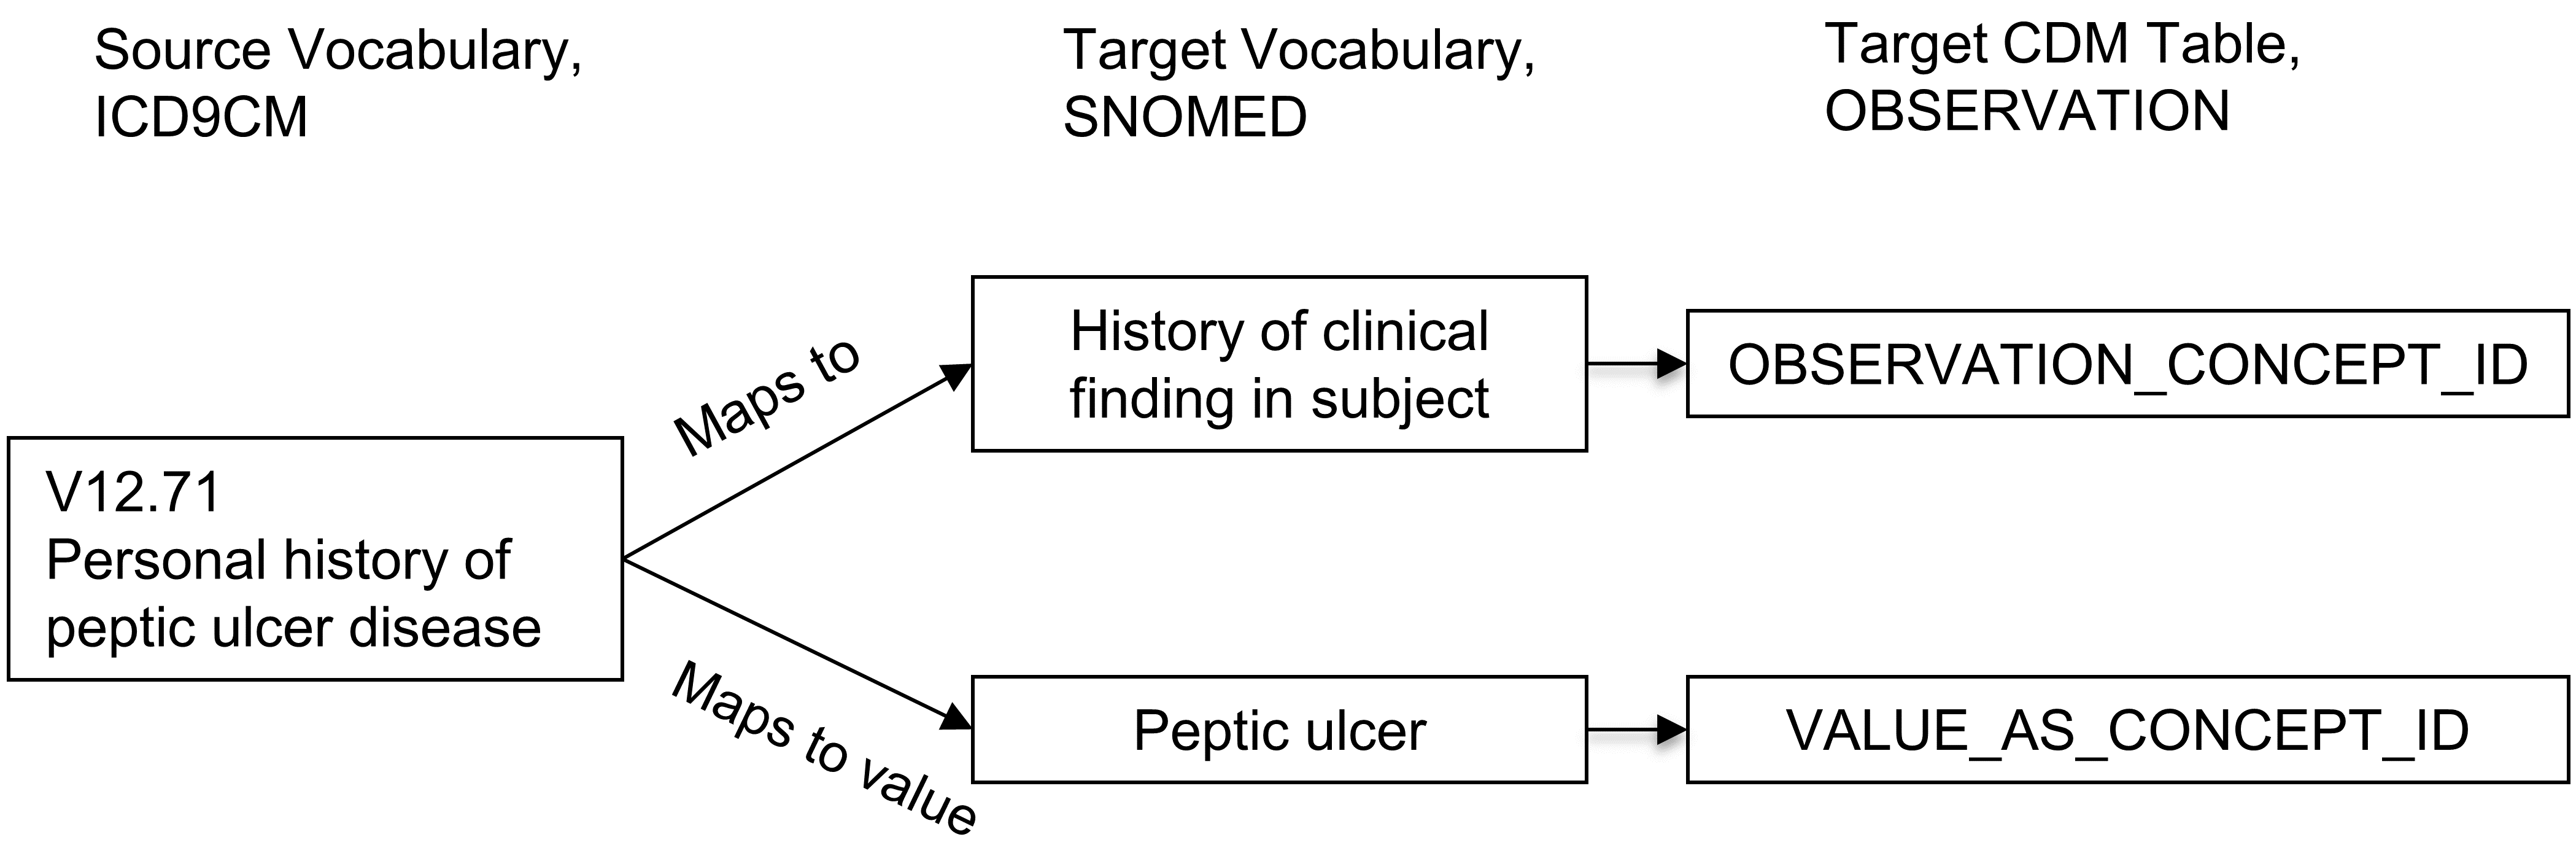
\includegraphics[width=1\linewidth]{images/StandardizedVocabularies/conceptValue} 

}

\caption{One-to-many mapping between source concept and Standard Concepts. A pre-coordinated concept is split into two concepts, one of which is the attribute (here history of clinical finding) and the other one is the value (peptic ulcer). While "Maps to" relationship will map to concepts of the measurement or observation domains, the ‘Maps to value" concepts have no domain restriction.}\label{fig:conceptValue}
\end{figure}

Mapping of concepts is another central feature of the OMOP Standardized
Vocabularies provided for free and supporting the efforts of the
community conducting Network Studies. Mapping relationships are derived
from external sources or maintained manually by the Vocabulary Team.
This means they are not perfect. If you find wrong or objectionable
mapping relationships it is crucial that you report and help improve the
process through a \href{https://forums.ohdsi.org}{Forums} or
\href{https://github.com/OHDSI/CommonDataModel/issues}{CDM issue} post.

A more detailed description of mapping conventions can be found in the
OHDSI Wiki.\footnote{\url{https://www.ohdsi.org/web/wiki/doku.php?id=documentation:vocabulary:mapping}}

\subsection{Hierarchical
Relationships}\label{hierarchical-relationships}

Relationships which indicate a hierarchy are defined through the ``Is
a'' - ``Subsumes'' relationship pair. Hierarchical relationships are
defined such that the child concept has all the attributes of the parent
concept, plus one or more additional attributes or a more precisely
defined attribute. For example, SNOMED 49436004 ``Atrial fibrillation''
is related to SNOMED 17366009 ``Atrial arrhythmia'' through a ``Is a''
relationship. Both concepts have an identical set of attributes except
the type of arrhythmia, which is defined as fibrillation in one but not
the other. Concepts can have more than one parent and more than one
child concept. In this example, SNOMED 49436004 ``Atrial fibrillation''
is also an ``Is a'' to SNOMED 40593004 ``Fibrillation.''
\index{concept!hierarchy}

\subsection{Relationships Between Concepts of Different
Vocabularies}\label{relationships-between-concepts-of-different-vocabularies}

These relationships are typically of the type ``Vocabulary A -
Vocabulary B equivalent'', which is either supplied by the original
source of the vocabulary or is built by the OHDSI Vocabulary team. They
may serve as approximate mappings but often times are less precise than
the better curated mapping relationships. High-quality equivalence
relationships (such as ``Source - RxNorm equivalent'') are always
duplicated by ``Maps to'' relationship.

\subsection{Relationships Between Concepts of the Same
Vocabulary}\label{relationships-between-concepts-of-the-same-vocabulary}

Internal vocabulary relationships are usually supplied by the vocabulary
provider. Full descriptions can be found in the vocabulary documentation
under the individual vocabulary at the OHDSI Wiki.\footnote{\url{https://www.ohdsi.org/web/wiki/doku.php?id=documentation:vocabulary}}

Many of these define relationships between clinical events and can be
used for information retrieval. For example, disorders of the urethra
can be found by following the ``Finding site of'' relationship (see
Table \ref{tab:findingSite}):

\begin{longtable}[]{@{}ll@{}}
\caption{\label{tab:findingSite} ``Finding site of'' relationship of the
``Urethra,'' indicating conditions that are situated all in the this
anatomical structure.}\tabularnewline
\toprule
CONCEPT\_ID\_1 & CONCEPT\_ID\_2\tabularnewline
\midrule
\endfirsthead
\toprule
CONCEPT\_ID\_1 & CONCEPT\_ID\_2\tabularnewline
\midrule
\endhead
4000504 ``Urethra part'' & 36713433 ``Partial duplication of
urethra''\tabularnewline
4000504 ``Urethra part'' & 433583 ``Epispadias''\tabularnewline
4000504 ``Urethra part'' & 443533 ``Epispadias, male''\tabularnewline
4000504 ``Urethra part'' & 4005956 ``Epispadias, female''\tabularnewline
\bottomrule
\end{longtable}

The quality and comprehensiveness of these relationships varies
depending on the quality in the original vocabulary. Generally,
vocabularies that are used to draw Standard Concepts from, such as
SNOMED, are chosen for the reason of their better curation and therefore
tend to have higher quality internal relationships as well.

\section{Hierarchy}\label{conceptAncestor}

Within a domain, standard and classification concepts are organized in a
hierarchical structure and stored in the CONCEPT\_ANCESTOR table. This
allows querying and retrieving concepts and all their hierarchical
descendants. These descendants have the same attributes as their
ancestor, but also additional or more defined ones.

The CONCEPT\_ANCESTOR table is built automatically from the
CONCEPT\_RELATIONSHIP table traversing all possible concepts connected
through hierarchical relationships. These are the ``Is a'' -
``Subsumes'' pairs (see Figure \ref{fig:conceptAncestor}), and other
relationships connecting hierarchies across vocabularies. The choice
whether a relationship participates in the hierarchy constructor is
defined for each relationship ID by the flag DEFINES\_ANCESTRY in the
RELATIONSHIP reference table.







\begin{figure}

{\centering 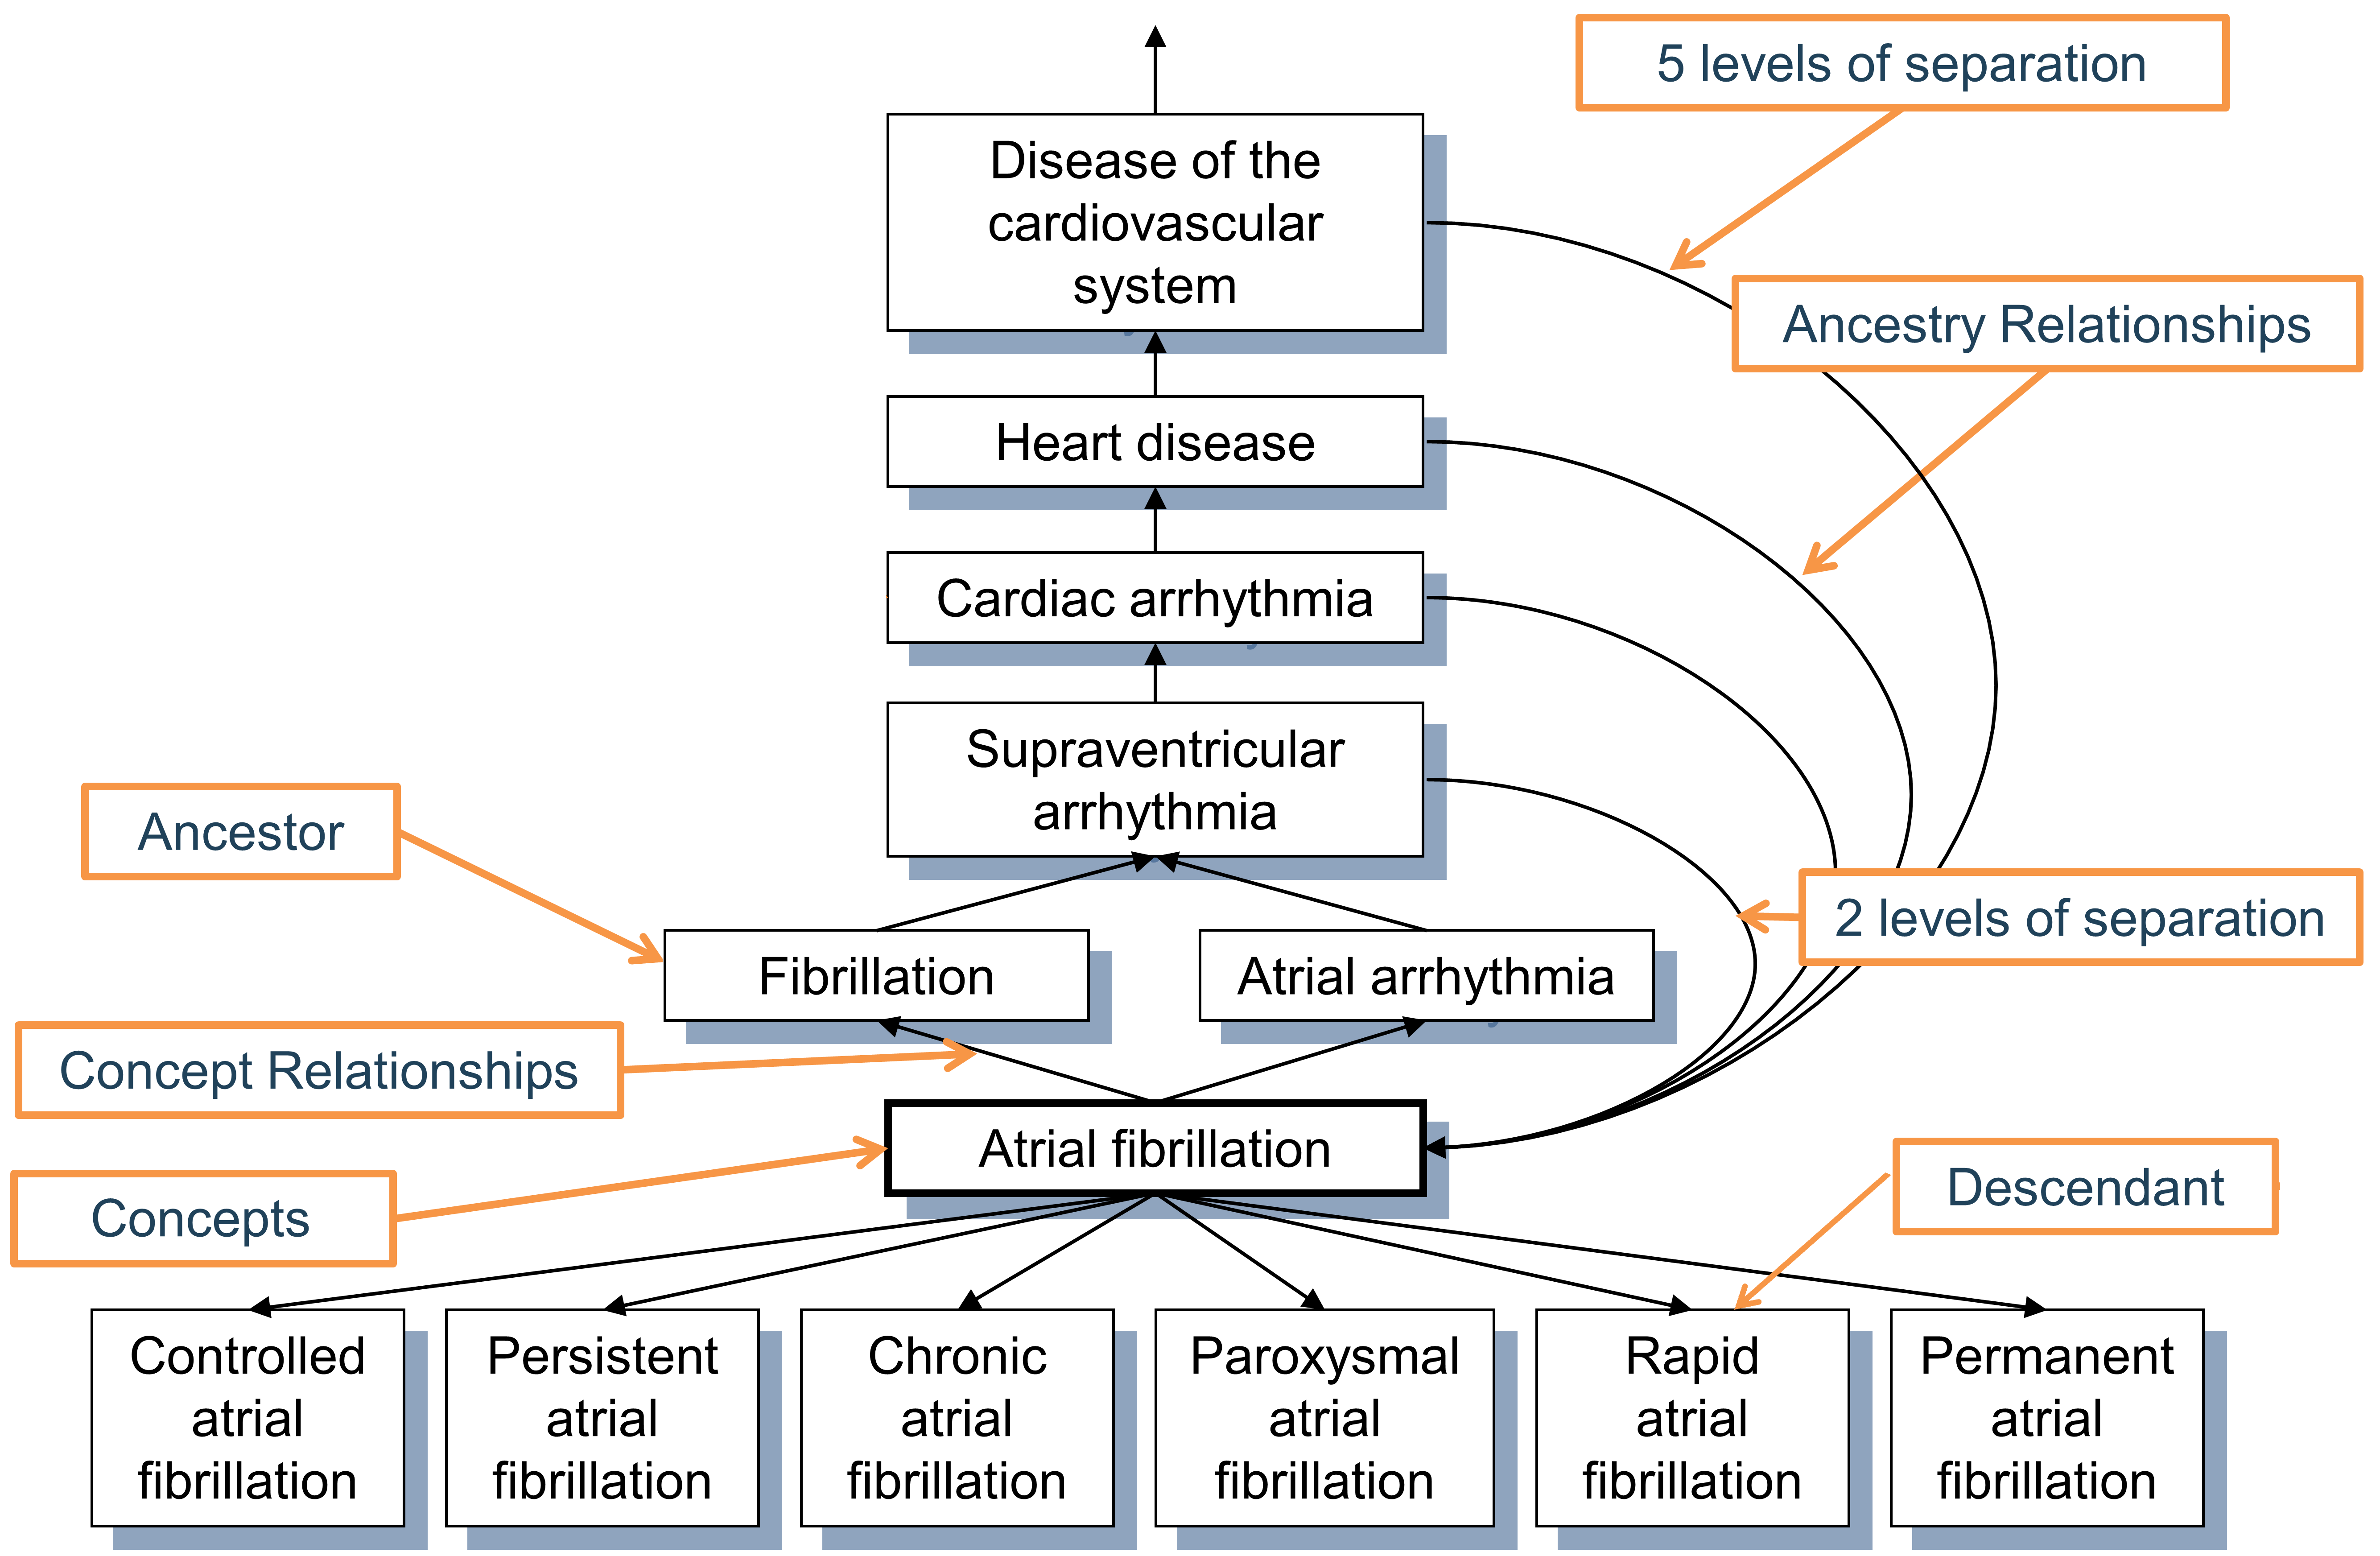
\includegraphics[width=1\linewidth]{images/StandardizedVocabularies/conceptAncestor} 

}

\caption{Hierarchy of the condition ``Atrial fibrillation.'' First
degree ancestry is defined through ``Is a'' and ``Subsumes''
relationships, while all higher degree relations are inferred and stored
in the CONCEPT\_ANCESTOR table. Each concept is also its own descendant
with both levels of separation equal to 0. \index{concept!ancestor}}\label{fig:conceptAncestor}
\end{figure}

The ancestral degree, or the number of steps between ancestor and
descendant, is captured in the MIN\_LEVELS\_OF\_SEPARATION and
MAX\_LEVELS\_OF\_SEPARATION fields, defining the shortest or longest
possible connection. Not all hierarchical relationships contribute
equally to the levels-of-separation calculation. A step counted for the
degree is determined by the IS\_HIERARCHICAL flag in the RELATIONSHIP
reference table for each relationship ID.

At the moment, a high-quality comprehensive hierarchy exists only for
two domains: drug and condition. Procedure, measurement and observation
domains are only partially covered and in the process of construction.
The ancestry is particularly useful for the drug domain as it allows
browsing all drugs with a given ingredient or members of drug classes
irrespective of the country of origin, brand name or other attributes.

\section{Internal Reference Tables}\label{internal-reference-tables}

DOMAIN\_ID, VOCABULARY\_ID, CONCEPT\_CLASS\_ID (all in CONCEPT records)
and CONCEPT\_RELATIONSHIP\_ID (in CONCEPT\_RELATIONSHIP) are all
controlled by their own vocabularies. They are defined in the four
reference tables DOMAIN, VOCABULARY, CONCEPT\_CLASS and RELATIONSHIP,
containing the *\_ID fields as primary keys, a more detailed *\_NAME
field and a *\_CONCEPT\_ID field with a reference back to the CONCEPT
table, which contains a concept for each of the reference table records.
The purpose of these duplicate records is to support an information
model allowing for automatic navigation engines.

The VOCABULARY table also contains the VOCABULARY\_REFERENCE and
VOCABULARY\_VERSION fields referring to the source and version of the
original vocabulary. The RELATIONSHIP table has the additional fields
DEFINES\_ANCESTRY, IS\_HIERARCHICAL and REVERSE\_RELATIONSHIP\_ID. The
latter defines the counter relationship ID for a pair of relationships.

\section{Special Situations}\label{specialSituations}

\subsection{Gender}\label{gender}

Gender in the OMOP CDM and Standardized Vocabularies denotes the
biological sex at birth. Often, questions are posed how to define
alternative genders. These use cases have to be covered through records
in the OBSERVATION table, where the self-defined gender of a person is
stored (if the data asset contains such information).

\subsection{Race and Ethnicity}\label{race-and-ethnicity}

These follow the definitions of how the US government defines this.
Ethnicity is a differentiation of Hispanic or non-Hispanic populations,
which can have any race. Race is divided into the common 5 top races,
which have ethnicities as their hierarchical descendants. Mixed races
are not included.

\subsection{Diagnostic Coding Schemes and OMOP
Conditions}\label{diagnostic-coding-schemes-and-omop-conditions}

Commonly used coding schemes such as ICD-9 or ICD-10 define more or less
well-defined diagnoses based on a proper diagnostic work-up. The
condition domain is not identical with this semantic space, but
partially overlapping. For example, conditions also contain signs and
symptoms that are recorded before a diagnosis is derived, and ICD codes
contain concepts that belong to other domains (e.g.~procedures).

\subsection{Procedure Coding Systems}\label{procedure-coding-systems}

Similarly, coding schemes like HCPCS and CPT4 are thought to be listings
of medical procedures. In reality, they are more like a menu of
justifications for payment for medical service. Many of these services
are subsumed under the procedure domain, but many concepts fall outside
this realm.

\subsection{Devices}\label{devices}

Device concepts have no standardized coding scheme that could be used to
source Standard Concepts. In many source data, devices are not even
coded or contained in an external coding scheme. For this same reason,
there is currently no hierarchical system available.

\subsection{Visits and Services}\label{visits-and-services}

Visits concepts define the nature of healthcare encounters. In many
source systems they are called Place of Service, denoting some
organization or physical structure, such as a hospital. In others, they
are called services. These also differ between countries, and their
definition is hard to obtain. Care sites are often specializing on one
of few visits (XYZ Hospital), but still should not be defined by them
(even in XYZ hospital patients might encounter non-hospital visits).

\subsection{Providers and Specialties}\label{providers-and-specialties}

Any human provider is defined in the provider domain. These can be
medical professionals such as doctors and nurses, but also non-medical
providers like optometrists or shoemakers. Specialties are descendants
of the provider ``Physician.'' Care Sites cannot carry a specialty, even
though they are often defined by the specialty of their main staff
(``Surgical department'').

\subsection{Therapeutic Areas With Special
Requirements}\label{therapeutic-areas-with-special-requirements}

The Standardized Vocabularies cover all aspects of healthcare in a
comprehensive fashion. However, some therapeutic areas have special
needs and require special vocabularies. Examples are oncology,
radiology, and genomics. Special OHDSI Working Groups develop these
extensions. As a result, the OMOP Standardized Vocabularies constitutes
an integrated system, where concepts from different origins and purposes
all reside in the same domain-specific hierarchies.

\subsection{Standard Concepts in the Drug Domain}\label{rxNormExtension}

Many concepts of the drug domain are sourced from RxNorm, a publicly
available vocabulary produced by the US National Library of Medicine.
However, drugs outside the US may or may not be covered, depending on
whether or not the combination of ingredient, form and strength is
marketed in the US. Drugs that are not on the US market are added by the
OHDSI Vocabulary Team under a vocabulary called
\href{https://www.ohdsi.org/web/wiki/doku.php?id=documentation:vocabulary:rxnorm_extension}{RxNorm
Extension}, which is the only large domain vocabulary produced by OHDSI.

\subsection{Flavors of NULL}\label{flavors-of-null}

Many vocabularies contain codes about absence of information. For
example, of the five gender concepts 8507 ``Male,'' 8532 ``Female,''
8570 ``Ambiguous,'' 8551 ``Unknown,'' and 8521 ``Other'', only the first
two are Standard, and the other three are source concepts with no
mapping. In the Standardized Vocabularies, there is no distinction made
why a piece of information is not available; it might be because of an
active withdrawal of information by the patient, a missing value, a
value that is not defined or standardized in some way, or the absence of
a mapping record in CONCEPT\_RELATIONSHIP. Any such concept is not
mapped, which corresponds to a default mapping to the Standard Concept
with the concept ID = 0.

\section{Summary}\label{summary-1}

\BeginKnitrBlock{rmdsummary}
\begin{itemize}
\tightlist
\item
  All events and administrative facts are represented in the OMOP
  Standardized Vocabularies as concepts, concept relationships, and
  concept ancestor hierarchy.
\item
  Most of these are adopted from existing coding schemes or
  vocabularies, while some of them are curated de-novo by the OHDSI
  Vocabulary Team.
\item
  All concepts are assigned a domain, which controls where the fact
  represented by the concept is stored in the CDM.
\item
  Concepts of equivalent meaning in different vocabularies are mapped to
  one of them, which is designated the Standard Concept. The others are
  source concepts.
\item
  Mapping is done through the concept relationships ``Maps to'' and
  ``Maps to value''.
\item
  There is an additional class of concepts called classification
  concepts, which are non-standard, but in contrast to source concepts
  they participate in the hierarchy.
\item
  Concepts have a life-cycle over time.
\item
  Concepts within a domain are organized into hierarchies. The quality
  of the hierarchy differs between domains, and the completion of the
  hierarchy system is an ongoing task.
\item
  You are strongly encouraged to engage with the community if you
  believe you found a mistake or inaccuracy.
\end{itemize}
\EndKnitrBlock{rmdsummary}

\section{Exercises}\label{exercises}

\subsubsection*{Prerequisites}\label{prerequisites}
\addcontentsline{toc}{subsubsection}{Prerequisites}

For these first exercises you will need to look up concepts in the
Standardized Vocabularies, which can be done through ATHENA\footnote{\url{http://athena.ohdsi.org/}}
or ATLAS.\footnote{\url{http://atlas-demo.ohdsi.org}}

\BeginKnitrBlock{exercise}
\protect\hypertarget{exr:exerciseVocab1}{}{\label{exr:exerciseVocab1} }What
is the Standard Concept ID for ``Gastrointestinal hemorrhage''?
\EndKnitrBlock{exercise}

\BeginKnitrBlock{exercise}
\protect\hypertarget{exr:exerciseVocab2}{}{\label{exr:exerciseVocab2} }Which
ICD-10CM codes map to the Standard Concept for ``Gastrointestinal
hemorrhage''? Which ICD-9CM codes map to this Standard Concept?
\EndKnitrBlock{exercise}

\BeginKnitrBlock{exercise}
\protect\hypertarget{exr:exerciseVocab3}{}{\label{exr:exerciseVocab3} }What
are the MedDRA preferred terms that are equivalent to the Standard
Concept for ``Gastrointestinal hemorrhage''?
\EndKnitrBlock{exercise}

Suggested answers can be found in Appendix \ref{Vocabanswers}.

\chapter{추출 변환 적재}\label{ExtractTransformLoad}

\emph{챕터 작성자 : Clair Blacketer \& Erica Voss}

\section{서론}

원천 데이터에서 OMOP 공통 데이터 모델(Common Data Model, CDM)을 얻기
위해서는 추출, 변환, 적재(Extract Transform Load, ETL) 절차가 필요하다.
이 절차는 데이터를 CDM으로 재구축 과정이며, 표준용어로의 매핑, SQL
코드들을 이용한 자동화된 절차로 이루어지게 된다. ETL 절차는 원천
데이터가 갱신될 때마다 언제든지 재수행 가능하게끔 반복 가능하게 구축하는
것이 중요하다. \index{ETL|see {extract, transform and load (ETL)}}
\index{raw data} \index{native data|see {raw data}}
\index{source data|see{raw data}}

ETL을 진행한다는 것은 많은 일들을 필요로 한다. 몇 년 동안의 과정을 통해
우리는 4가지 단계들로 이루어진 최상의 단계들을 개발하였다.

\begin{enumerate}
\def\labelenumi{\arabic{enumi}.}
\tightlist
\item
  데이터 전문가와 CDM 전문가가 함게 ETL을 설계할 것.
\item
  의학 지식이 있는 사람들이 코드 매핑을 작업할 것.
\item
  기술자가 ETL을 수행할 것.
\item
  모든 사람이 질 관리에 참여할 것.
\end{enumerate}

이 챕터에서 우리는 각 단계들을 세부적으로 살펴볼 것이다. 각 절차들을
보조하기 위해 다양한 도구들이 OHDSI 커뮤니티에 의해 개발되어왔고, 이
도구들에 대해서도 다룰 것이다. 마지막으로 CDM과 ETL의 유지에 관해
이야기하며 마무리할 것이다.

\section{1단계 : ETL 설계}\label{-etl-}

ETL 설계와 ETL 수행을 명확하게 분리하는 것은 중요하다. ETL을 설계하는
것은 원천 데이터와 CDM 모두에 대한 넓은 지식을 필요로 한다. 반대로 ETL을
수행할 때는 ETL을 기술적인 측면에서 효율적으로 수행하는 방법에 대해 기술
전문가들에게 의존하게 된다. 만약 동시에 두 가지 모두를 진행하려 한다면,
전체적인 그림에 집중할 때보다 세부적인 사항에서 막히게 될 가능성이 높다.

두 가지의 밀접하게 연관된 도구들이 ETL 설계를 위해 개발되었다: 흰 토끼
(White Rabbit), 모자 속 토끼 (Rabbit-in-a-Hat)

\subsection{흰 토끼 (White Rabbit)}\label{--white-rabbit}

ETL 절차를 시작하기 위해서는 테이블, 필드, 내용을 포함한 데이터에 대한
이해가 필요하다. 하단의 링크에
\href{https://github.com/OHDSI/WhiteRabbit}{White Rabbit}에 대한 정보가
기록되어 있다. White Rabbit은 장기적인 보건의료 데이터베이스의
\href{https://github.com/OHDSI/CommonDataModel}{OMOP CDM}으로의 ETL 작업
준비를 도와주기 위한 소프트웨어이다. White Rabbit은 데이터를 탐색하고
ETL 설계를 시작하기 위한 필수적인 정보들에 대한 보고서를 생성해준다.
모든 소스 코드와 설치 방법 뿐만 아니라 설명서는 깃헙(Github)에서 확인
가능하다.\footnote{\url{https://github.com/OHDSI/WhiteRabbit}.}
\index{White Rabbit} \index{data profiling|see {White Rabbit}}

\subsubsection*{범위와 목표}\label{-}
\addcontentsline{toc}{subsubsection}{범위와 목표}

White Rabbit의 주요 기능은 원천 데이터에 대한 탐색을 수행하고, 테이블,
필드, 필드값들에 대한 세부적인 정보를 제공하는 것이다. 원천 데이터는
comma-seperated 텍스트 파일일 수도 있고, 데이터베이스(MySQL, SQL Server,
Oracle, PostgreSQL, Microsoft APS, Microsoft Access, Amazon RedShift)에
적재되어 있을 수도 있다. 탐색 과정에서 Rabbit-In-a-Hat 도구와 함께
쓴다면 ETL을 설계할 때 참고할 수 있는 보고서를 생성할 수 있다. White
Rabbit은 다른 표준 데이터 프로파일링 도구들과는 달리 개인 식별
정보(Personally Identifiable Information, PII)가 결과 데이터 파일에서
보여지는 것을 방지한다.

\subsubsection*{절차 개요}\label{-}
\addcontentsline{toc}{subsubsection}{절차 개요}

원천 데이터를 탐색하기 위해 소프트웨어를 사용하는 일반적인 순서:

\begin{enumerate}
\def\labelenumi{\arabic{enumi}.}
\tightlist
\item
  로컬 컴퓨터에서의 결과를 내보낼 작업 폴더를 설정.
\item
  데이터베이스 혹은 CSV 텍스트 파일과의 연결 및 연결 확인.
\item
  탐색 대상 테이블 선택 및 탐색.
\item
  White Rabbit의 원천 데이터에 대한 정보 생성 및 내보내기.
\end{enumerate}

\subsubsection*{작업 폴더 설정}\label{--}
\addcontentsline{toc}{subsubsection}{작업 폴더 설정}

White Rabbit 어플리케이션의 다운로드 및 설치 이후, 처음으로 할 일은 작업
폴더를 설정하는 것이다. White Rabbit이 생성하는 모든 파일들은 설정한
로컬 폴더에 생성될 것이다. 그림 \ref{fig:WhiteRabbitLocation}에서
보여지는 ``Pick Folder'' 버튼을 사용하여 탐색 문서들이 저장될 로컬
환경을 탐색할 수 있다.

\begin{figure}

{\centering 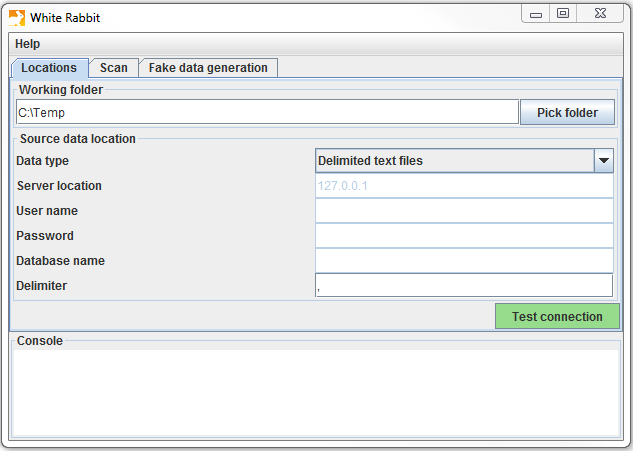
\includegraphics[width=1\linewidth]{images/ExtractTransformLoad/WhiteRabbitLocation} 

}

\caption{The "Pick Folder" button allows the specification of a working folder for the White Rabbit application.}\label{fig:WhiteRabbitLocation}
\end{figure}

\subsubsection*{데이터베이스 연결}\label{-}
\addcontentsline{toc}{subsubsection}{데이터베이스 연결}

White Rabbit은 구분된 텍스트 파일들과 데이터베이스를 지원한다. 다양한
필드들에 대한 필요 항목들의 설명을 보려면 마우스를 올려야한다. 더욱
자세한 설명은 설명서에서 확인할 수 있다.

\subsubsection*{데이터베이스의 테이블 탐색}\label{--}
\addcontentsline{toc}{subsubsection}{데이터베이스의 테이블 탐색}

데이터베이스에 연결한 이후에는 데이터베이스에 적재되어있는 테이블들을
탐색할 수 있다. 탐색 과정은 ETL을 설계하는데 도움을 되는 원천 데이터에
대한 정보를 담은 보고서를 생성할 수 있다. 그림
\ref{fig:WhiteRabbitAddTables}에 보이는 Scan 탭의 ``Add'' (Ctrl + mouse
click) 버튼을 눌러서 선택된 원천 데이터베이스의 각 테이블들을
선택하거나, ``Add all in DB'' 누름으로써 모든 테이블들을 자동적으로
선택할 수 있다.

\begin{figure}

{\centering 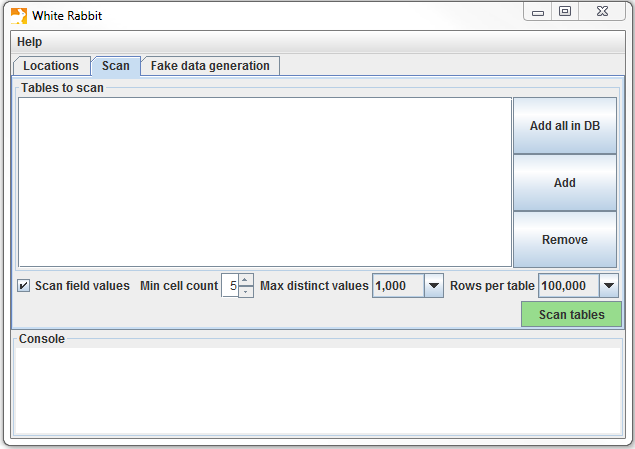
\includegraphics[width=1\linewidth]{images/ExtractTransformLoad/WhiteRabbitAddTables} 

}

\caption{White Rabbit Scan tab.}\label{fig:WhiteRabbitAddTables}
\end{figure}

탐색에 사용될 몇 가지 옵션들:

\begin{itemize}
\tightlist
\item
  ``Scan field values'' 는 열에 어떠한 값들을 나타나는지 보고싶을때
  사용한다.
\item
  ``Min cell count'' 는 필드값을 탐색할 때 쓰이는 옵션이다. 기본값은 5로
  설정되어 있으며, 이는 원천 데이터에서 5번 이하로 나타나는 값들은
  보고서에 나타내지 않는 것을 의미한다. 각 데이터셋들은 각각의 고유한
  규칙에 따라 minimal cell count가 정해져야할 것이다.
\item
  ``Rows per table'' 는 필드값을 탐색할 때 쓰이는 옵션이다. 기본값으로
  White Rabbit은 테이블에서 무작위로 100,000개의 행렬을 선택하여 탐색할
  것이다.
\end{itemize}

모든 옵션들이 설정된 이후에는 ``Scan tables''을 누르면 된다. 탐색이
완료된 이후에는 보고서가 작업 폴더에 생성될 것이다.

\subsubsection*{탐색 보고서의 이해}\label{--}
\addcontentsline{toc}{subsubsection}{탐색 보고서의 이해}

탐색이 완료된 이후에는 선택된 작업 폴더에 엑셀 파일이 생성될 것이며,
엑셀 파일에는 스캔한 각 테이블에 대한 하나의 탭과 개요 탭이 생성된다.
개요 탭은 탐색한 모든 테이블들이며, 각 테이블의 필드, 각 필드의 데이터
타입, 필드의 최대 길이, 테이블의 행의 수, 탐색한 행의 수, 그리고 얼마나
많은 필드들이 비어있었는지 보여준다. 그림 \ref{fig:ScanOverviewTab}은
개요 탭의 예시를 보여준다.

\begin{figure}

{\centering 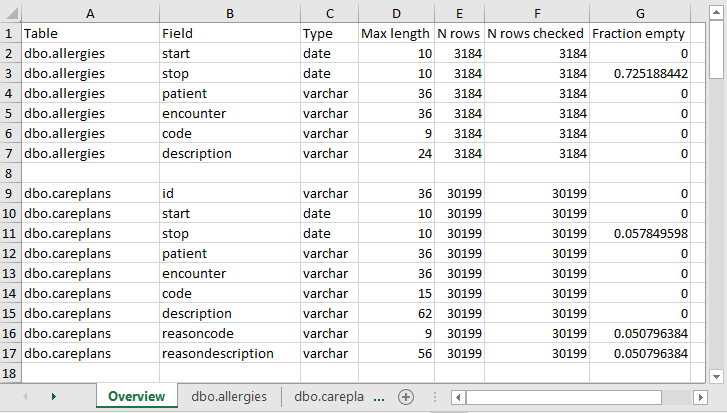
\includegraphics[width=1\linewidth]{images/ExtractTransformLoad/ScanOverviewTab} 

}

\caption{Example overview tab from a scan report.}\label{fig:ScanOverviewTab}
\end{figure}

각 테이블들의 탭들은 각각의 필드, 필드의 값들, 그리고 값들의 빈도를
나타낸다. 각 원천 테이블의 컬럼들은 엑셀에서 두 개의 컬럼들로 생성된다.
하나는 탐색 시 설정한 ``Min cell count'' 보다 큰 값들의 고유한 값을
보여준다. 만약 고유한 값 목록이 잘려있다면, 목록의 마지막 값은 ``List
truncated'' 가 될 것이다; 이는 하나 혹은 그 이상의 값들이 ``Min cell
count'' 보다 작은 고유한 값이 있음을 나타낸다. 각각의 고유한 값 옆에는
빈도를 나타내는 두 번째 컬럼이 있다(표본에서 값이 발생하는 횟수). 이 두
컬럼들(고유한 값과 빈도 수)은 작업책(workbook)의 프로파일링된 테이블의
모든 원천 변수들에 대해 반복되서 나타난다.

\begin{figure}

{\centering 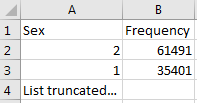
\includegraphics[width=0.3\linewidth]{images/ExtractTransformLoad/ScanSex} 

}

\caption{Example values for a single column.}\label{fig:scanSex}
\end{figure}

보고서는 원천 데이터에 무엇이 있는지를 강조함으로써 데이터를 이해하는데
강력한 도움을 준다. 예를 들면, 그림 \ref{fig:scanSex}에 나타난 결과가
탐색된 테이블 컬럼 중 하나인 ``Sex''에 반환될 경우, 우리는 각각
61,491번과 35,401번 나타난 공통된 값들(1과 2)이 있음을 알 수 있다. White
Rabbit은 1을 남성으로, 2를 여성으로 정의하지는 않을 것이다; 데이터
소유자가 일반적으로 원천 시스템에 고유한 원천 코드를 정의해야한다.
하지만 이 두 가지 값(1 \& 2)들은 데이터에 있는 유일한 값들이 아니기
때문에 우리는 잘린 목록을 확인해야한다. 이 값들은 (``Min cell count''
정의에 따라) 매우 낮은 빈도로 나타나게 되고, 종종 부정확하거나 매우
의심스러운 값들로 표현된다. ETL 수행을 계획할 때 우리는 높은 빈도의 성별
개념로써 1과 2만 다루는 것이 아니라, 컬럼에 존재하는 낮은 빈도의 값들도
고려해야한다. 예를 들어 만약 낮은 빈도의 성별들이 ``NULL''일 경우 ETL
진행 시 이러한 데이터에 대해 어떻게 처리할 것인지 확실히 해야한다.

\subsection{모자 속 토끼 (Rabbit-In-a-Hat)}\label{---rabbit-in-a-hat}

White Rabbit과 함께 우리는 원천 데이터에 대한 분명한 그림을 그릴 수
있다. 또한 우리는 CDM에 대한 전체 명세서를 알고 있다. 이제 우리는
하나에서 다른 하나로 넘어갈 로직을 정의해야한다. 이 설계 활동은 원천
데이터와 CDM 모두에 대한 온전한 지식을 요구한다. White Rabbit
소프트웨어와 함께 사용되는 Rabbit-in-a-Hat 도구는 명확하게 이 분야의
전문가들을 위해 개발되었다. 일반적으로 ETL 설계팀은 회의실에 같이 앉아
Rabbit-in-a-Hat을 프로젝터 화면으로 같이 보면서 작업을 한다. 첫 번째로
테이블 간의 매핑은 협력적으로 결정될 수 있으며, 그 후에는 필드 간의
매핑이 설계되는 동시에 어떤한 값들을 변환시킬지 로직을 정의할 수 있다.
\index{Rabbit-In-A-Hat} \index{ETL design|see {Rabbit-In-A-Hat}}

\subsubsection*{범위와 목표}\label{--1}
\addcontentsline{toc}{subsubsection}{범위와 목표}

Rabbit-In-a-Hat은 White Rabbit의 탐색 문서들을 읽고 나타내기 위해
설계되었다. White Rabbit은 원천 데이터에 대한 정보를 생성하는반면,
Rabbit-In-a-Hat은 그 정보를 사용하고 그래픽 사용자 인터페이스를 통하여
사용자들로 하여금 원천 데이터의 테이블과 컬럼들을 CDM으로 연결시게끔
해준다. Rabbit-In-a-Hat은 ETL 절차에 대한 문서를 생성해주지만 ETL을 위한
코드는 생성하지 않는다.

\subsubsection*{절차 개요}\label{--1}
\addcontentsline{toc}{subsubsection}{절차 개요}

소프트웨어를 이용한 ETL 문서 생성을 위한 일반적인 순서:

\begin{enumerate}
\def\labelenumi{\arabic{enumi}.}
\tightlist
\item
  WhiteRabbit의 탐색 완료 결과.
\item
  탐색 결과 확인; 인터페이스가 원천 테이블들과 CDM 테이블들을 보여줌.
\item
  원천 테이블들의 정보와 상응하는 CDM 테이블들의 연결.
\item
  CDM 테이블에 상응하는 각 원천 테이블들에 대해서 세부적인 원천 컬럼과
  CDM 컬럼의 연결을 정의.
\item
  Rabbit-In-a-Hat 작업을 저장하고 MS 워드 문서로 내보내기.
\end{enumerate}

\subsubsection*{ETL 로직 작성}\label{etl--}
\addcontentsline{toc}{subsubsection}{ETL 로직 작성}

일단 Rabbit-In-a-Hat 내의 White Rabbit 탐색 보고서를 확인한다면, 원천
데이터를 OMOP CDM으로 변환하는 설계와 로직 작성을 시작할 준비가 된다.
하나의 예시로써 하단의 챕터들에서 Synthea\footnote{Synthea\textsuperscript{TM}
  is a patient generator that aims to model real patients. Data are
  created based on parameters passed to the application.The structure of
  the data can be found here:
  \url{https://github.com/synthetichealth/synthea/wiki}.} 데이터베이스의
일부 테이블들의 변환을 보여줄 것이다.

\subsubsection*{ETL의 일반적인 흐름}\label{etl--}
\addcontentsline{toc}{subsubsection}{ETL의 일반적인 흐름}

CDM이 사람 중심의 모델이기 때문에 PERSON 테이블 먼저 매핑을 시작하는
것이 좋다. 모든 임상적 사건과 관련있는 테이블들(CONDITION\_OCCURRENCE,
DRUG\_EXPOSURE, PROCEDURE\_OCCURRENCE 기타 등.)은 PERSON 테이블의
person\_id를 참조하기에 PERSON 테이블에 대한 로직을 먼저 작성하는 것이
나중을 위해 좋다. PERSON 테이블을 변환한 다음에는 OBSERVATION\_PERIOD를
변환하는 것이 좋은 선택이다. CDM 데이터베이스의 각 사람들은 최소한
하나의 OBSERVATION\_PERIOD를 가져야하고, 일반적으로 한 사람에 대한 모든
사건들은 이 관측시기 내에 맞춰지게 된다. PERSON과 OBSERVATION\_PERIOD
테이블들이 완료되면 보통 PROVIDER, CARE\_SITE, 그리고 LOCATION과 같은
디멘션 테이블(dimensional table)들이 다음 대상이 된다. 임상 테이블
이전에 마지막으로 로직을 작성해야하는 테이블은 VISIT\_OCCURRENCE이다. 한
사람의 환자로써의 여정에서 대부분의 사건들이 방문할 때 발생하기 때문에
종종 모든 ETL 과정에서 가장 복잡하고 중요한 부분이기도 하다. 일단 이
테이블들이 완료되면 어떤 CDM 테이블들 어떤 순서대로 매핑할 지는 선택하기
나름이다.

\begin{figure}

{\centering 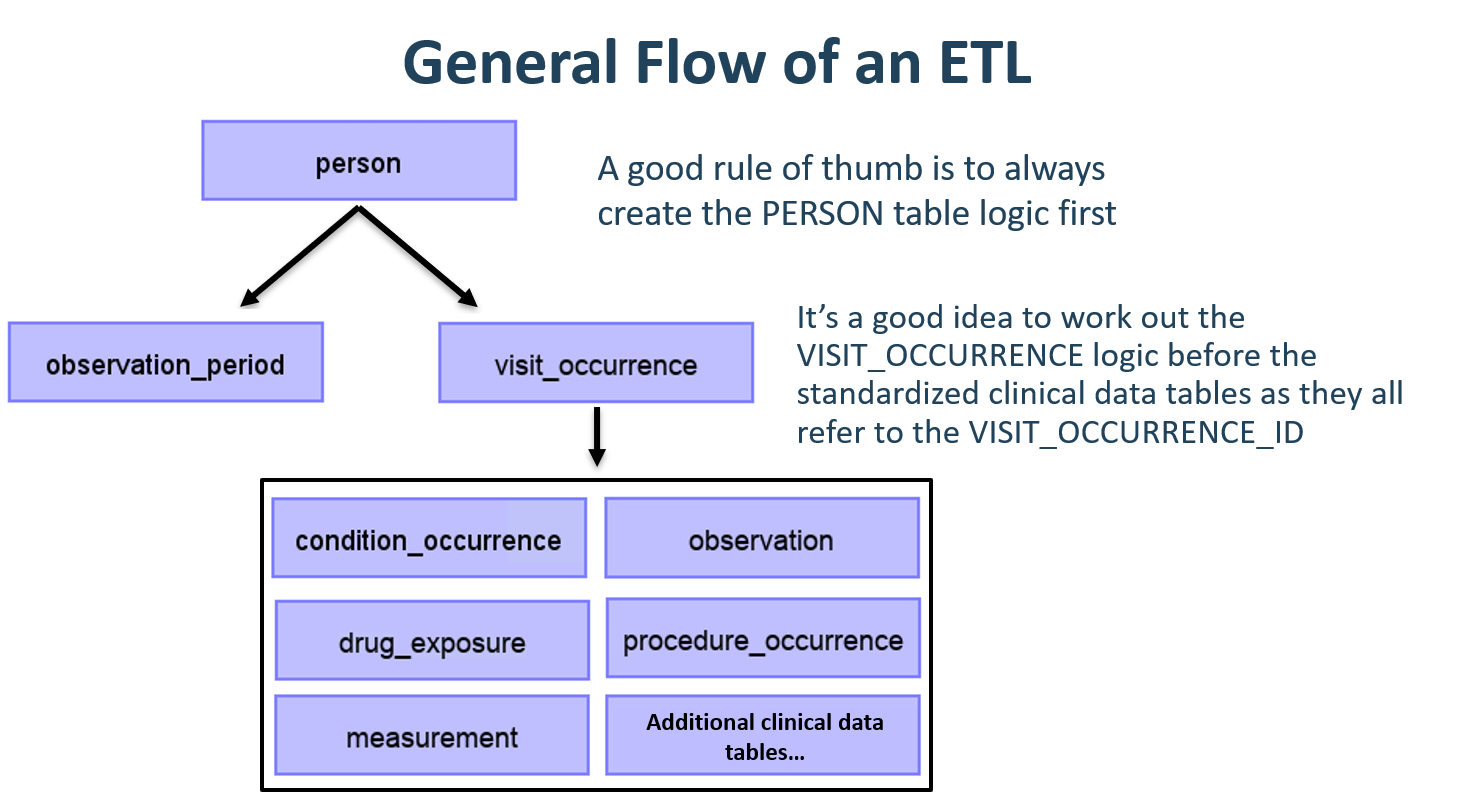
\includegraphics[width=1\linewidth]{images/ExtractTransformLoad/flowOfEtl} 

}

\caption{General flow of an ETL and which tables to map first.}\label{fig:etlFlow}
\end{figure}

CDM 변환 과정에서 종종 중간 테이블들을 만들 필요가 있을 수 있다. 올바른
VISIT\_OCCURRENCE\_ID들을 해당 사건들에 부여하거나 아니면 원천 코드를
표준 코드로 매핑하는 경우들일 수도 있다(이 단계는 종종 매우 느리게
진행된다). 중간 테이블들은 100\% 허용되고 장려된다. 하지만 이러한 중간
테이블들이 변환이 완료된 이후에도 남아있거나 사용되는 것은 장려되지
않는다.

\subsubsection*{매핑 예시: PERSON 테이블}\label{--person-}
\addcontentsline{toc}{subsubsection}{매핑 예시: PERSON 테이블}

Synthea 데이터 구조에서 환자 테이블은 20개의 열들을 갖고 있지만 그림
\ref{fig:syntheaPerson}에서 보이는 것처럼 모든 열들이 PERSON 테이블에
필요한 것은 아니다. 이런 일은 매우 흔한 일이고 문제가 되지 않는다. 이
예시에서는 환자 이름, 운전면허번호, 여권 번호 등 Synthea의 환자 테이블의
많은 데이터 포인트들이 CDM PERSON 테이블에 사용되지 않는 것을 알 수
있다.

\begin{figure}

{\centering 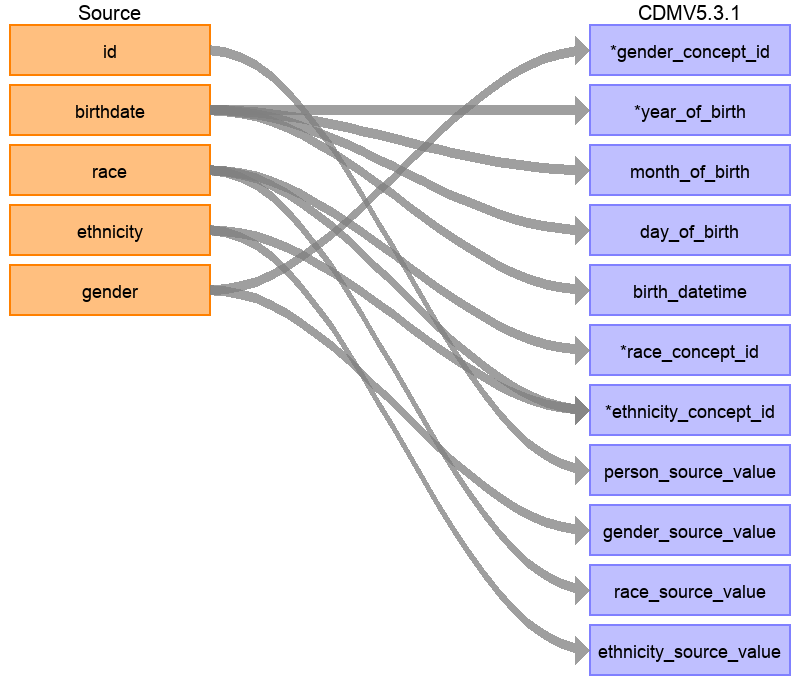
\includegraphics[width=1\linewidth]{images/ExtractTransformLoad/syntheaPersonTable} 

}

\caption{Mapping of Synthea Patients table to CDM PERSON table.}\label{fig:syntheaPerson}
\end{figure}

하단의 표 \ref{tab:syntheaEtlPerson}는 Synthea의 환자 테이블이 CDM
PERSON 테이블로 변환되는 로직을 보여준다. `Destination Field'는 CDM
데이터의 어디에 매핑되는지를 나타낸다. `Source field'는 원천
테이블(예시에서는 환자 테이블)의 어느 열에서 CDM의 열로 변하는지
나타낸다. 마지막으로, `Logic \& comments'는 로직에 대한 설명을 의미한다.

\begin{longtable}[]{@{}lll@{}}
\caption{\label{tab:syntheaEtlPerson} ETL logic to convert the Synthea
Patients table to CDM PERSON table.}\tabularnewline
\toprule
\begin{minipage}[b]{0.28\columnwidth}\raggedright\strut
Destination Field\strut
\end{minipage} & \begin{minipage}[b]{0.13\columnwidth}\raggedright\strut
Source field\strut
\end{minipage} & \begin{minipage}[b]{0.50\columnwidth}\raggedright\strut
Logic \& comments\strut
\end{minipage}\tabularnewline
\midrule
\endfirsthead
\toprule
\begin{minipage}[b]{0.28\columnwidth}\raggedright\strut
Destination Field\strut
\end{minipage} & \begin{minipage}[b]{0.13\columnwidth}\raggedright\strut
Source field\strut
\end{minipage} & \begin{minipage}[b]{0.50\columnwidth}\raggedright\strut
Logic \& comments\strut
\end{minipage}\tabularnewline
\midrule
\endhead
\begin{minipage}[t]{0.28\columnwidth}\raggedright\strut
PERSON\_ID\strut
\end{minipage} & \begin{minipage}[t]{0.13\columnwidth}\raggedright\strut
\strut
\end{minipage} & \begin{minipage}[t]{0.50\columnwidth}\raggedright\strut
Autogenerate. The PERSON\_ID will be generated at the time of
implementation. This is because the id value from the source is a
varchar value while the PERSON\_ID is an integer. The id field from the
source is set as the PERSON\_SOURCE\_VALUE to preserve that value and
allow for error-checking if necessary.\strut
\end{minipage}\tabularnewline
\begin{minipage}[t]{0.28\columnwidth}\raggedright\strut
GENDER\_CONCEPT\_ID\strut
\end{minipage} & \begin{minipage}[t]{0.13\columnwidth}\raggedright\strut
gender\strut
\end{minipage} & \begin{minipage}[t]{0.50\columnwidth}\raggedright\strut
When gender = `M' then set GENDER\_CONCEPT\_ID to 8507, when gender =
`F' then set to 8532. Drop any rows with missing/unknown gender. These
two concepts were chosen as they are the only two standard concepts in
the gender domain. The choice to drop patients with unknown genders
tends to be site-based, though it is recommended they are removed as
people without a gender are excluded from analyses.\strut
\end{minipage}\tabularnewline
\begin{minipage}[t]{0.28\columnwidth}\raggedright\strut
YEAR\_OF\_BIRTH\strut
\end{minipage} & \begin{minipage}[t]{0.13\columnwidth}\raggedright\strut
birthdate\strut
\end{minipage} & \begin{minipage}[t]{0.50\columnwidth}\raggedright\strut
Take year from birthdate\strut
\end{minipage}\tabularnewline
\begin{minipage}[t]{0.28\columnwidth}\raggedright\strut
MONTH\_OF\_BIRTH\strut
\end{minipage} & \begin{minipage}[t]{0.13\columnwidth}\raggedright\strut
birthdate\strut
\end{minipage} & \begin{minipage}[t]{0.50\columnwidth}\raggedright\strut
Take month from birthdate\strut
\end{minipage}\tabularnewline
\begin{minipage}[t]{0.28\columnwidth}\raggedright\strut
DAY\_OF\_BIRTH\strut
\end{minipage} & \begin{minipage}[t]{0.13\columnwidth}\raggedright\strut
birthdate\strut
\end{minipage} & \begin{minipage}[t]{0.50\columnwidth}\raggedright\strut
Take day from birthdate\strut
\end{minipage}\tabularnewline
\begin{minipage}[t]{0.28\columnwidth}\raggedright\strut
BIRTH\_DATETIME\strut
\end{minipage} & \begin{minipage}[t]{0.13\columnwidth}\raggedright\strut
birthdate\strut
\end{minipage} & \begin{minipage}[t]{0.50\columnwidth}\raggedright\strut
With midnight as time 00:00:00. Here, the source did not supply a time
of birth so the choice was made to set it at midnight.\strut
\end{minipage}\tabularnewline
\begin{minipage}[t]{0.28\columnwidth}\raggedright\strut
RACE\_CONCEPT\_ID\strut
\end{minipage} & \begin{minipage}[t]{0.13\columnwidth}\raggedright\strut
race\strut
\end{minipage} & \begin{minipage}[t]{0.50\columnwidth}\raggedright\strut
When race = `WHITE' then set as 8527, when race = `BLACK' then set as
8516, when race = `ASIAN' then set as 8515, otherwise set as 0. These
concepts were chosen because they are the standard concepts belonging to
the race domain that most closely align with the race categories in the
source.\strut
\end{minipage}\tabularnewline
\begin{minipage}[t]{0.28\columnwidth}\raggedright\strut
ETHNICITY\_ CONCEPT\_ID\strut
\end{minipage} & \begin{minipage}[t]{0.13\columnwidth}\raggedright\strut
race ethnicity\strut
\end{minipage} & \begin{minipage}[t]{0.50\columnwidth}\raggedright\strut
When race = `HISPANIC', or when ethnicity in (`CENTRAL\_AMERICAN',
`DOMINICAN', `MEXICAN', `PUERTO\_RICAN', `SOUTH\_AMERICAN') then set as
38003563, otherwise set as 0. This is a good example of how multiple
source columns can contribute to one CDM column. In the CDM ethnicity is
represented as either Hispanic or not Hispanic so values from both the
source column race and source column ethnicity will determine this
value.\strut
\end{minipage}\tabularnewline
\begin{minipage}[t]{0.28\columnwidth}\raggedright\strut
LOCATION\_ID\strut
\end{minipage} & \begin{minipage}[t]{0.13\columnwidth}\raggedright\strut
\strut
\end{minipage} & \begin{minipage}[t]{0.50\columnwidth}\raggedright\strut
\strut
\end{minipage}\tabularnewline
\begin{minipage}[t]{0.28\columnwidth}\raggedright\strut
PROVIDER\_ID\strut
\end{minipage} & \begin{minipage}[t]{0.13\columnwidth}\raggedright\strut
\strut
\end{minipage} & \begin{minipage}[t]{0.50\columnwidth}\raggedright\strut
\strut
\end{minipage}\tabularnewline
\begin{minipage}[t]{0.28\columnwidth}\raggedright\strut
CARE\_SITE\_ID\strut
\end{minipage} & \begin{minipage}[t]{0.13\columnwidth}\raggedright\strut
\strut
\end{minipage} & \begin{minipage}[t]{0.50\columnwidth}\raggedright\strut
\strut
\end{minipage}\tabularnewline
\begin{minipage}[t]{0.28\columnwidth}\raggedright\strut
PERSON\_SOURCE\_ VALUE\strut
\end{minipage} & \begin{minipage}[t]{0.13\columnwidth}\raggedright\strut
id\strut
\end{minipage} & \begin{minipage}[t]{0.50\columnwidth}\raggedright\strut
\strut
\end{minipage}\tabularnewline
\begin{minipage}[t]{0.28\columnwidth}\raggedright\strut
GENDER\_SOURCE\_ VALUE\strut
\end{minipage} & \begin{minipage}[t]{0.13\columnwidth}\raggedright\strut
gender\strut
\end{minipage} & \begin{minipage}[t]{0.50\columnwidth}\raggedright\strut
\strut
\end{minipage}\tabularnewline
\begin{minipage}[t]{0.28\columnwidth}\raggedright\strut
GENDER\_SOURCE\_ CONCEPT\_ID\strut
\end{minipage} & \begin{minipage}[t]{0.13\columnwidth}\raggedright\strut
\strut
\end{minipage} & \begin{minipage}[t]{0.50\columnwidth}\raggedright\strut
\strut
\end{minipage}\tabularnewline
\begin{minipage}[t]{0.28\columnwidth}\raggedright\strut
RACE\_SOURCE\_ VALUE\strut
\end{minipage} & \begin{minipage}[t]{0.13\columnwidth}\raggedright\strut
race\strut
\end{minipage} & \begin{minipage}[t]{0.50\columnwidth}\raggedright\strut
\strut
\end{minipage}\tabularnewline
\begin{minipage}[t]{0.28\columnwidth}\raggedright\strut
RACE\_SOURCE\_ CONCEPT\_ID\strut
\end{minipage} & \begin{minipage}[t]{0.13\columnwidth}\raggedright\strut
\strut
\end{minipage} & \begin{minipage}[t]{0.50\columnwidth}\raggedright\strut
\strut
\end{minipage}\tabularnewline
\begin{minipage}[t]{0.28\columnwidth}\raggedright\strut
ETHNICITY\_ SOURCE\_VALUE\strut
\end{minipage} & \begin{minipage}[t]{0.13\columnwidth}\raggedright\strut
ethnicity\strut
\end{minipage} & \begin{minipage}[t]{0.50\columnwidth}\raggedright\strut
In this case the ETHNICITY\_SOURCE\_VALUE will have more granularity
than the ETHNICITY\_CONCEPT\_ID.\strut
\end{minipage}\tabularnewline
\begin{minipage}[t]{0.28\columnwidth}\raggedright\strut
ETHNICITY\_ SOURCE\_CONCEPT\_ID\strut
\end{minipage} & \begin{minipage}[t]{0.13\columnwidth}\raggedright\strut
\strut
\end{minipage} & \begin{minipage}[t]{0.50\columnwidth}\raggedright\strut
\strut
\end{minipage}\tabularnewline
\bottomrule
\end{longtable}

Synthea 데이터의 CDM으로의 변환에 대한 더 자세한 설명은 전체 명세서를
참고하면 된다.\footnote{\url{https://ohdsi.github.io/ETL-Synthea/}}

\section{2 단계: 코드 매핑 생성}\label{---}

점점 더 많은 원천 코드들이 OMOP 용어에 추가되어지고 있다. 이것은 CDM으로
변환된 데이터의 코딩 체계가 이미 CDM에 포함되거나 매핑되었을 수도 있다는
것을 의미한다. OMOP Vocabulary의 VOCABULARY 테이블을 통해 어떤 용어들이
포함되었는지 확인할 수 있다. 비표준인 원천 코드들(e.g.~ICD-10CM
codes)에서 표준용어들(e.g.~SNOMED codes)로의 매핑을 확인하려면
CONCEPT\_RELATIONSHIP 테이블 내의 relationship\_id = ``Maps to'' 인
값들을 찾으면 확인할 수 있다. 예를 들면 ICD-10CM 코드 `I21' (``Acute
Myocardial Infarction'')의 표준용어 ID를 확인하기 위해 다음과 같은 SQL을
사용할 수 있다:

\begin{Shaded}
\begin{Highlighting}[]
\KeywordTok{SELECT}\NormalTok{ concept_id_2 standard_concept_id}
\KeywordTok{FROM}\NormalTok{ concept_relationship}
\KeywordTok{INNER} \KeywordTok{JOIN}\NormalTok{ concept source_concept}
  \KeywordTok{ON}\NormalTok{ concept_id = concept_id_}\DecValTok{1}
\KeywordTok{WHERE}\NormalTok{ concept_code = }\StringTok{'I21'}
  \KeywordTok{AND}\NormalTok{ vocabulary_id = }\StringTok{'ICD10CM'}
  \KeywordTok{AND}\NormalTok{ relationship_id = }\StringTok{'Maps to'}\NormalTok{; }
\end{Highlighting}
\end{Shaded}

\begin{longtable}[]{@{}r@{}}
\toprule
STANDARD\_CONCEPT\_ID\tabularnewline
\midrule
\endhead
312327\tabularnewline
\bottomrule
\end{longtable}

하지만 가끔은 원천 데이터가 Vocabulary에 없는 코딩 시스템을 사용할 수도
있다. 이러한 경우에는 원천 코딩 시스템의 Standard Concept으로의 매핑을
정의하여야한다. 하지만 원천 코딩 시스템에 많은 수의 용어들이 있을 경우
코드 매핑이 어려울 수도 있다. 이를 쉽게 진행하기 위한 몇 가지
참고사항들이 있다.

\begin{itemize}
\tightlist
\item
  가장 높은 빈도의 코드들에 집중하라. 절대 쓰이지 않는 코드나 거의 안
  쓰이는 코드들은 실제 연구에서도 안 쓰이기 때문에 많은 노력을 들여서
  매핑을 진행할 필요가 없다.
\item
  가능하면 기존의 정보들을 활용하라. 예를 들어서 많은 국가 약물 코딩
  시스템은 이미 ATC로 매핑되어있다. 비록 ATC가 많은 목적에 대해
  세부적으로 부합하지는 않지만, ATC와 RxNorm의 관계를 통해 어떤 RxNorm
  코드들이 사용되는지 추측할 수는 있다.
\item
  우사기(Usagi)를 사용하라.
\end{itemize}

\subsection{우사기(Usagi)}\label{usagi}

우사기(Usagi)는 코드 매핑의 절차를 도와주는 도구이다. Usagi는 코드
설명의 단어 유사도에 기반하여 매핑을 추천할 수 있다. 만약 원천 코드가
외국어로만 확인 가능하다면, Google Translate\footnote{\url{https://translate.google.com/}}를
통해 종종 해당 용어들의 훌륭한 영어 번역을 확인할 수 있다. Usagi는
사용자들로 하여금 자동 추천이 정확하지 않을 경우 적절한 목표 개념을 찾을
수 있도록 하고 있다. 최종적으로 사용자는 어떤 매핑이 ETL에 사용될 수
있는지 지정할 수 있다. Usagi는 GitHub\footnote{\url{https://github.com/OHDSI/Usagi}}을
통해 사용할 수 있다. \index{Usagi}
\index{source code mapping|see {Usagi}}

\subsubsection*{범위와 목표}\label{--2}
\addcontentsline{toc}{subsubsection}{범위와 목표}

매핑이 필요한 원천 코드들은 Usagi로 불러올 수 있다(만약 코드들이 영어가
아닐경우, 추가적으로 번역된 열들이 필요하다). 단어 유사도 접근법은 원천
코드와 Vocabulary 개념들을 연결시키기 위해 필요하다.하지만 이러한 코드
연결은 수동적으로 검토해야하고, Usagi는 이를 수행하기 위한 인터페이스를
제공한다. Usagi는 Vocabulary에 Standard인 concept들만을 제안한다.

\subsubsection*{절차 개요}\label{--2}
\addcontentsline{toc}{subsubsection}{절차 개요}

소프트웨어를 사용하기 위한 일반적인 순서:

\begin{enumerate}
\def\labelenumi{\arabic{enumi}.}
\tightlist
\item
  원천 시스템(``원천 코드'')로부터 Vocabulary concepts들로의 매핑을
  진행하고 싶은 코드들을 올림.
\item
  Usagi 단어 유사도 접근법을 이용하여 Vocabulary concepts들로의 매핑을
  진행.
\item
  Usagi 인터페이스를 활용하여 제안된 매핑을 확인하고 필요할 경우 개선.
\item
  매핑 결과를 Vocabulary의 SOURCE\_TO\_CONCEPT\_MAP으로 내보냄.
\end{enumerate}

\subsubsection{Usagi로의 원천 코드 가져오기}\label{usagi---}

원천 시스템에서 CSV나 엑셀(.xlsx) 파일로 원천 코드들을 내보낸다. 이 때
파일은 원천 코드와 영어 코드 설명에 대한 열들이 있어야하지만, 추가적인
정보들 역시 더해질 수 있다(e.g.~약물 용량, 번역되었을 경우 원래 언어로의
코드 설명). 게다가 원천 코드에 대한 정보 뿐만 아니라, 어떤 코드를 먼저
매핑해야할지 정하는데 도움이 되기 때문에 빈도 역시 포함되있는 것이
좋다(e.g.~1,000개의 원천 코드를 가져올 수 있지만, 100개만 실제 시스템에
정말로 사용되는 경우). 만약 원천 코드가 영어로의 번역이 필요할 경우,
Google Translate이 도움이 될 수 있다.

참고: 원천 코드는 도메인(domain)에 의해 분류되어야하며, 하나의 파일로
묶여서는 안됨.

파일로부터 원천 코드를 Usagi로 올린다 -\textgreater{} 코드 메뉴를
가져온다. 여기서 ``Import codes \ldots{}''는 그림
\ref{fig:usagiImport}과 같이 보일 것이다. 이 그림에서 원천 코드 용어들은
네덜란드어이고, 영어로 번역되어있다. Usagi는 표준용어로의 매핑을 위해
영어 번역을 이용할 것이다.

\begin{figure}

{\centering 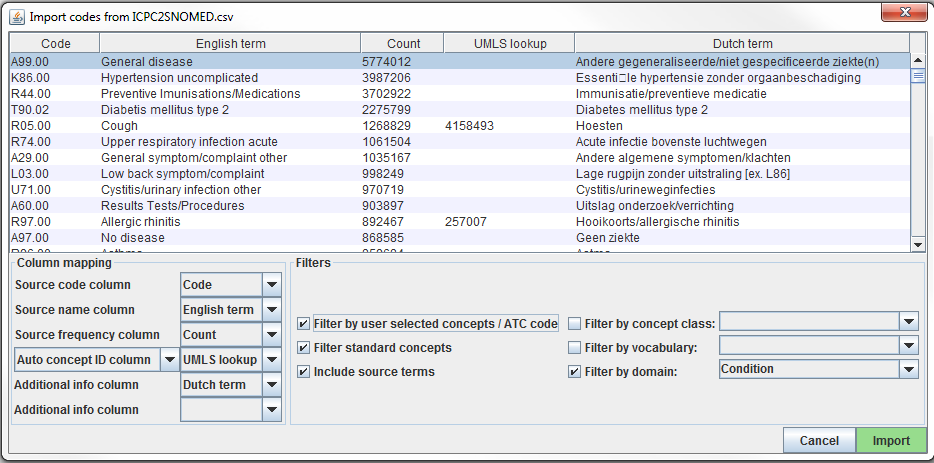
\includegraphics[width=1\linewidth]{images/ExtractTransformLoad/usagiImport} 

}

\caption{Usagi source code input screen.}\label{fig:usagiImport}
\end{figure}

``Column mapping'' 부분(왼쪽 아래)은 Usagi로 하여금 불러온 테이블을
어떻게 사용할 것인지 정하는 단계이다. 만약 마우스를 끌어다 놓으면, 각
컬럼들을 정의하는 팝업창이 나타날 것이다. Usagi는 원천 코드를 Vocaublary
concept 코드에 연결시키는 정보로써 ``Additional info'' 컬럼을 사용하지
않을 것이다; 하지만 이 추가적인 정보는 개인이 원천 코드 매핑을
검토하는데 도움을 줄 수 있기에 포함되어야 한다.

마지막으로 ``Filters'' 부분(아래 오른쪽)에서 Usagi로 매핑할 때의 몇 가지
제한을 설정할 수 있다. 예를 들어 그림 \ref{fig:usagiImport}에서 사용자는
Condition 도메인에만 원천 코드를 매핑하고 있다. 기본적으로 Usagi는
Standard Ceoncepts에만 매핑을 진행하지만, 만약 ``Filter standard
concepts'' 옵션이 아닐 경우, Usagi는 Classification Concepts 또한 검토할
것이다. 마우스를 다른 필터에 올려놓으면 해당 필터에 대한 추가적인 정보가
나타날 것이다.

한 가지 특별한 필터는 ``Filter by automatically selected concepts / ATC
code''이다. 만약 검색에 조건을 걸어야 한다면, 자동 concept ID로 표시되는
컬럼(세미콜론으로 구분)에 CONCEPT\_ID 목록이나 ATC 코드를을 제공하여
하면 된다. 예를 들어 약물의 경우 이미 각 약들에 ATC 코드가 이미 할당되어
있을 수 이따. 비록 ATC 코드가 하나의 RxNorm 약물 코드로 인지되지
않더라도, Vocabulary의 ATC 코드 한정으로 검색을 제한하는데 도와줄 수
있다. ATC 코드를 사용하려면 다음 절차를 따르면 된다:

\begin{enumerate}
\def\labelenumi{\arabic{enumi}.}
\tightlist
\item
  컬럼 매핑 부분에서, ``Auto concept ID column''을 ``ATC column''로
  바꾸어라.
\item
  컬럼 매핑 부분에서, ATC 코드가 포함된 열을 ``ATC column''으로
  선택하여라.
\item
  ``Filter by user selected concepts / ATC code'' 필터를 눌러라.
\end{enumerate}

또한 ATC 코드 이외의 다른 것들로도 조건을 설정할 수 있다. 위의 그림
예시에서 보여지듯이 우리는 UMLS의 부분 매핑을 이용하여 Usagi의 검색을
설정하였다. 이런 경우에는 ``Auto concept ID column''을 사용하여야 한다.

일단 모든 설정을 마치고 나면, ``Import'' 버튼을 눌러서 파일을
불러와야한다. 파일 불러오기를 할 때 단어 유사도 알고리즘을 이용하여 원천
코드를 매핑하기 때문에 대략 몇 분 정도 소요될 수 있다.

\subsubsection*{원천 코드의 Vocabulary Concept 매핑
검토}\label{--vocabulary-concept--}
\addcontentsline{toc}{subsubsection}{원천 코드의 Vocabulary Concept 매핑
검토}

일단 원천 코드의 파일을 불러오면, 매핑 절차가 시작된다. 그림
\ref{fig:usagiOverview}에서 Usagi 화면이 3가지 주요 기능으로 구분된 것을
확인할 수 있다: 개요 테이블, 선택된 매핑 테이블, 검색 기능. 이 때, 오른
클릭을 하여 어떤 테이블에 대해서도 컬럼들을 선택하여 숨기거나 가려서
시각적 복잡성을 줄일 수 있다는 것을 참고하면 된다.

\begin{figure}

{\centering 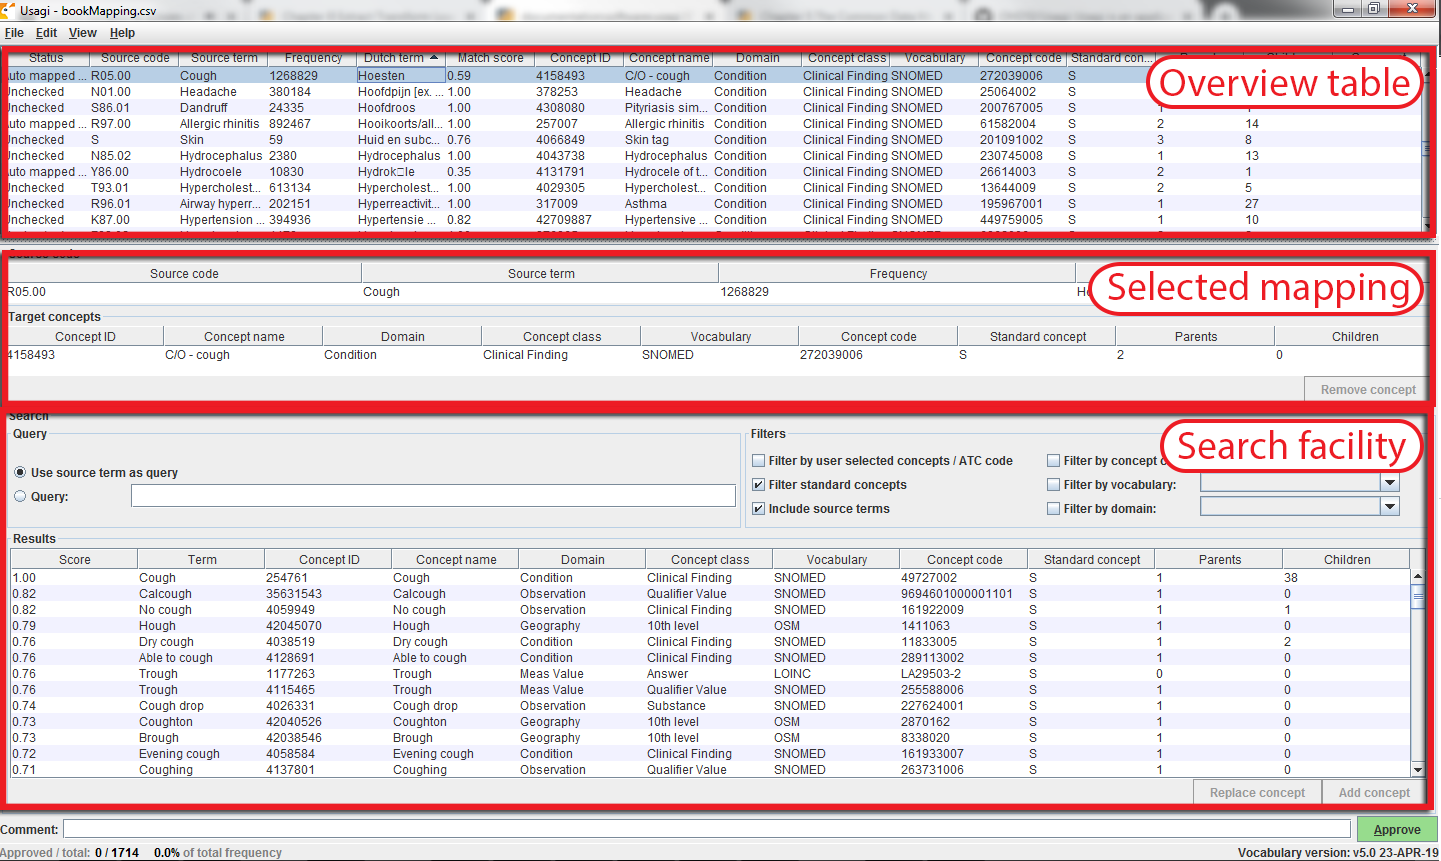
\includegraphics[width=1\linewidth]{images/ExtractTransformLoad/usagiOverview} 

}

\caption{Usagi source code input screen.}\label{fig:usagiOverview}
\end{figure}

\subsubsection*{제안된 매핑의 승인}\label{--}
\addcontentsline{toc}{subsubsection}{제안된 매핑의 승인}

``Overview Table''은 현재의 원천 코드의 매핑을 보여준다. 원천 코드를
불러온 직후, 검색 설정과 단어 유사도를 기반으로 자동으로 생성되고
제안되는 매핑을 포함하고 있다. 그림 \ref{fig:usagiOverview}에서
나타나듯이, 사용자가 검색 옵션을 Condition으로 설정했기에 네덜란드어
Condition 코드의 영어 이름은 Condition 도메인의 표준용어로 매핑되는 것을
볼 수 있다. Usagi는 원천 코드 기술서의 컨셉 이름과 동의어를 비교함으로써
최적의 매칭을 수행한다. 사용자가 ``Include source terms''를 선택하였기
때문에 Usagi는 vocabulary의 특정 코드로 매핑되는 모든 원천 코드의 이름과
동의어까지 검토하게 된다. 만약 Usagi가 매핑을 진행할 수 없을 경우,
CONCEPT\_ID = 0 으로 매핑될 것이다.

코딩 시스템에 익숙한 사람이 원천 코드의 표준 용어로의 매핑을 도와주는
것이 권장된다. 각 개인은 ``Overview Table'' 탭에서 각 코드에 대하여
Usagi가 권장하는 매핑을 받아들이거나 아니면 새로운 매핑을 선택하는
작업을 하게 된다. 예를 들어 그림 \ref{fig:usagiOverview}에서 우리는
네덜란드어 ``Hoesten''가 영어 ``Cough''로 번역되는 것을 볼 수 있다.
Usagi는 ``Cough''를 사용하고 Vocabualry 개념 ``4158493-C/O - cough''로
매핑을 한다. 이 때의 매핑에 대하여 매칭 점수는 0.58(매칭 점수는
일반적으로 0에서 1의 값을 가짐)이였고, 이는 Usagi가 이 네덜란드어에
대하여 SNOMED에 대해 매핑한 결과에 대해 확실하게 제시하기 어렵다는 것을
의미한다. 이 예시에서는 해당 매핑 결과에 동의하였고, 화면의 하단 우측의
``Approve'' 버튼을 클릭함으로써 승인하였다.

\subsubsection*{새로운 매핑의 탐색}\label{--}
\addcontentsline{toc}{subsubsection}{새로운 매핑의 탐색}

Usagi가 제시해주는 매핑에 대하여 사용자가 새로운 매핑을 찾거나 아니면
컨셉이 없도록(CONCEPT\_ID = 0) 하는 경우들도 있을 것이다. 그림
\ref{fig:usagiOverview}의 예시를 통해 네덜란드어 ``Hoesten''가 영어
``Cough''로 번역되는 것을 확인할 수 있었다. Usagi의 제안은 UMLS에서
파생된 매핑으로 제한되기에, 그 결과가 적합하지 않을 수도 있다. 검색
기능을 통해서 실제 용어 자체 혹은 검색 상자 쿼리를 이용해서 다른
컨셉들을 찾을 수 있다.

메뉴얼 검색 상자를 이용할 때, Usagi는 구조화된 검색 쿼리를 지원하지 않고
fuzzy search를 한다는 것을 기억하여야 한다. 그리고 현재까지는 AND나 OR과
같은 Boolean 연산자에 대해서는 검색을 지원하지 않고 있다.

``Cough''에 대해서 더 나은 매핑을 찾는다고 가정해보자. 검색 기능의
오른편 쿼리 부분에 Vocabulary 검색을 할 때 결과를 정리해주는 기능을
제공하는 필터 부분이 있다. 이러한 경우에는 우리는 표준 용어만을 찾아야
하며, 표준 용어에 매핑되는 코드의 이름과 동의어를 기반으로 검색할 수
있다.

이러한 검색 기준을 적용한다면 ``254761-Cough''과 같은 코드를 찾을 수
있으며, 이는 네덜란드어의 코드 매핑에 적합한 용어일 수도 있다. 이를
적용하기 위해 ``Selected Source Code'' 업데이트의 ``Replace concept''
버튼을 누르고, ``Approve'' 버튼을 누르면 된다. 또한 ``Add concept''
버튼이 있는데, 이는 하나의 원천 코드에 대한 다수의 표준 용어 개념 매핑을
할 수 있게 해준다(e.g.일부 원천 코드들은 표준 용어와는 달리 다양한
질병들을 함께 포함하고 있을 수 있다).

\subsubsection*{개념 정보}\label{-}
\addcontentsline{toc}{subsubsection}{개념 정보}

적절한 개념을 찾아 매핑을 하려 할 때, 컨셉의 ``social life''을 고려하는
것은 중요하다. 개념의 의미는 계층 구조에서의 위치에 따라 부분적으로
의존적일 수 있으며, 종종 계층적 지위와 거의 혹은 전혀 상관없고 대상
컨셉으로도 적절하지 않은 ``orphan concepts''들도 있다. Usagi는 각 개념에
대해 얼마나 많은 부모, 자식 개념들이 있는지 알려주기도 하고, ALT + C를
누르거나 위쪽 메뉴바의 view -\textgreater{} Concept을 누르면 더 자세한
정보를 볼 수 있게 해준다.

\begin{figure}

{\centering 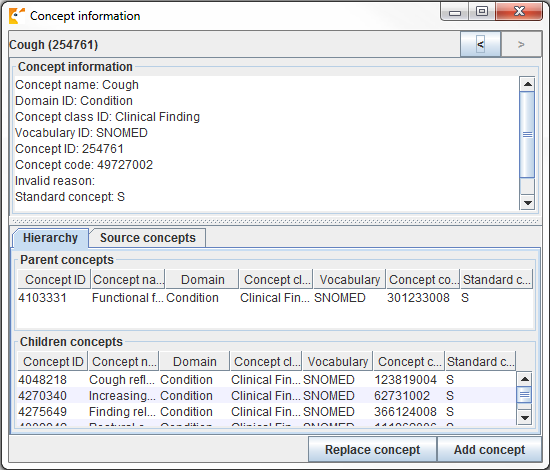
\includegraphics[width=1\linewidth]{images/ExtractTransformLoad/usagiConceptInfo} 

}

\caption{Usagi concept information panel.}\label{fig:usagiConceptInfo}
\end{figure}

그림 \ref{fig:usagiConceptInfo}은 개념 정보 패널을 보여준다. 개념의
일반적인 정보부터, 부모, 자식, 그리고 다른 원천 코드들과의 정보도
보여준다. 사용자는 이 패널을 이용해서 계층 구조를 탐색할 수 있고, 다른
목표 컨셉을 정할 수도 있다.

모든 코드가 끝날 때까지 코드를 따라 이 절차를 진행하면 된다. 화면의 맨
위의 원천 코드 목록에서, 열 머리글 별로 코드들을 정렬할 수 있다. 종종
최빈도부터 최저빈도의 코드까지 살펴보는 것을 권장한다. 화면의 하단 왼쪽
편에는 매핑을 허용한 코드들의 개수, 그리고 그에 따라 얼마나 많은
코드들이 발생했는지를 확인할 수 있다.

또한 매핑 결정에 대한 설명을 추가하여 문서화 시에 사용할 수도 있다.

\subsubsection*{최적의 절차}\label{-}
\addcontentsline{toc}{subsubsection}{최적의 절차}

\begin{itemize}
\tightlist
\item
  코딩 스키마에 경험이 있는 사람이 할 것
\item
  ``Overview Table''의 컬럼들을 컬럼 이름을 눌러서 정렬할 수 있다.
  ``Match Score''를 눌러서 정렬하는 것이 중요할 수도 있다; Usagi가 가장
  확실하게 제안하는 매핑 코드들을 검토하면 많은 코드들이의 작업이 빠르게
  끝날 수도 있다. 그리고 빈도가 높은 단어와 낮은 단어들에 쓰이는 노력이
  각각 다르기 때문에 ``Frequency''로 정렬해서 작업하는 것도 중요하다.
\item
  CONCEPT\_ID= 0으로 매핑하는 것도 괜찮지만, 어떤 코드들은 최적의 매핑
  코드들이 없을 수도 있고, 어떤 것들은 단지 마땅한 코드들이 없어서 일
  수도 있다.
\item
  특히 부모 계층과 자녀 계층에 대해서는 개념의 내용을 고려하는 것이
  중요하다.
\end{itemize}

\subsubsection*{Usagi 매핑 내보내기}\label{usagi--}
\addcontentsline{toc}{subsubsection}{Usagi 매핑 내보내기}

일단 USAGI를 통해 매핑을 생성하였으면, 이를 사용하기 가장 좋은 방법은
매핑을 내보낸 다음 Vocabulary의 SOURCE\_TO\_CONCEPT\_MAP 테이블에
추가하는 것이다.

매핑을 내보내기 위해서는, File -\textgreater{} Export
source\_to\_concept\_map으로 가면 된다. 이 때 어느
SOURCE\_VOCABULARY\_ID를 이용할 것인지 묻는 팝업창이 나타나는데 짧은
식별자를 입력하면 된다. Usagi는 입력된 식별자를 이용할 것이다.
SOURCE\_VOCABULARY\_ID가 SOURCE\_TO\_CONCEPT\_MAP 테이블의 특정 매핑을
식별할 수 있게끔 할 수 있다.

SOURCE\_VOCABULARY\_ID를 선택한 후에는, 내보낼 CSV 파일의 이름과 파일
경로를 입력하게 된다. 내보내는 CSV 파일의 구조는
SOURCE\_TO\_CONCEPT\_MAP 테이블과 동일하다. 이 매핑은 Vocabulary의
SOURCE\_TO\_CONCEPT 테이블로 추가될 수 있다. 그리고 앞선 단계에서 정의한
SOURCE\_VOCABULARY\_ID를 정의하는 VOCABULARY 테이블에 단일 행으로
추가하는 것이 좋다. 마지막으로, ``Approved'' 상태인 매핑들만을 CSV
파일로 내보내는 것이 중요하다; 매핑을 내보내기 위해서는 USAGI에서 매핑을
완료해야만 한다.

\subsubsection*{Usagi 매핑 업데이트}\label{usagi--}
\addcontentsline{toc}{subsubsection}{Usagi 매핑 업데이트}

매핑은 종종 한 번에 끝나지 않는다. 원천 코드가 추가되는 식으로 데이터가
업데이트 되거나 용어가 정기적으로 업데이트되면 매핑 또한 업데이트 되어야
할 것이다.

원천 코드가 업데이트될 때는 다음과 같은 단계들을 따르는 것이 좋다:

\begin{enumerate}
\def\labelenumi{\arabic{enumi}.}
\tightlist
\item
  새로운 원천 코드 파일을 불러온다.
\item
  파일을 고른다 -\textgreater{} 이전의 매핑을 적용시키고, 예전의 Usagi
  매핑 파일을 선택한다.
\item
  이전의 매핑 파일에서 매핑되지 않았던 코드들을 식별하고, 새롭게
  매핑한다.
\end{enumerate}

용어가 업데이트 되면 아래의 단계를 따른다:

\begin{enumerate}
\def\labelenumi{\arabic{enumi}.}
\tightlist
\item
  Athena에서 새로운 용어 파일들을 다운받는다.
\item
  Usagi 인덱스를 새로 빌딩한다(Help -\textgreater{} Rebuild index).
\item
  매핑 파일을 연다.
\item
  새로운 용어 버전에 따라 표준 용어가 아닌 코드들을 식별하여 적절한 목표
  컨셉들을 찾는다.
\end{enumerate}

\section{3 단계: ETL 수행}\label{-etl-}

일단 설계와 코드 매핑이 완료된다면, ETL 절차는 소프트웨어를 통해 수행
가능하다. ETL이 설계될 때, CDM과 원천 데이터 둘 다에 대해 잘 아는 사람이
참여하기를 권장하였다. 마찬가지로 ETL이 수행될 때도, 데이터(특히
빅데이터)와 ETL 수행 경험이 있는 사람이 참여하는 것이 바람직하다. 즉,
이건 그룹 외부의 기술 전문가를 고용하거나 초청하여 ETL 수행을 시키는
것일 수도 있다. 또한 이건 한 번에 끝나는 작업이 아니라는 점을 참고하기
바란다. 그렇기에 앞으로는 ETL 수행 및 유지에 일정 시간 이상을 할애할 수
있는 사람이나 팀이 있는 것이 좋을 것이다(\ref{CDMandETLMaintenance}에서
더 명확히 설명할 것이다).

수행은 각 기관에 따라 다양한 양상을 보이며 특히 인프라, 데이터베이스의
크기, ETL의 복잡성, 기술 전문가의 능력 등의 요소에 따라 많이 달라진다.
많은 요소들에 따라 달라지기 때문에 OHDSI는 ETL을 수행하기 위한 최선의
방법에 대한 공식적인 권고를 하고 있지 않다. 그 동안 많은 그룹들이 SQL
builders, SAS, C\#, Java, Kettle들을 사용해왔다. 각각 장점들과 단점들이
있었고, 그 어느 것도 이러한 기술에 익숙한 사람이 없으면 아무것도 사용할
수 없었다.

각각 다른 ETL의 예시들 (복잡성에 따라 정렬됨):

\begin{itemize}
\tightlist
\item
  ETL-Synthea - SQL을 이용한 Synthea 데이터베이스 변환
\item
  \url{https://github.com/OHDSI/etl-synthea}
\item
  ETL-CDMBuilder - 다수의 데이터베이스를 변환하기 위해 고안된 .NET
  application
\item
  \url{https://github.com/OHDSI/etl-cdmbuilder}
\item
  ETL-LambdaBuilder - AWS lamda 기능을 이용한 빌더
\item
  \url{https://github.com/OHDSI/etl-lambdabuilder}
\end{itemize}

그동안 많은 시도들이 있었지만, `ultimate'한 사용자 친화적인 ETL 도구를
개발하는데에는 포기했다. 항상 많은 경우에 이러한 도구들은 ETL 작업의
80\%까지는 잘 수행하지만, 남은 20\%에 있어서는 원천 데이터베이스에 따라
low-level에서의 코드 작성이 필요하다.

일단 기술 전문가가 수행할 준비가 된다면, ETL 설계 문서가 그들과
공유되어야만 한다. 문서에는 수행을 시작할만한 충분한 정보가
있어야하지만, 항상 개발자들이 개발 과정 중에 ETL 설계자들에게 질문할 수
있는 환경 역시 마련되있어야한다. ETL 설계자들에게는 로직이 명확해
보일지라도 CDM이나 데이터에 친숙하지 않은 수행자들에게는 명확하지 않아
보일 수도 있다. 그렇기에 수행 단계는 팀으로써 수행하여야 한다.
설계자들과 수행자들 모두 로직이 올바르게 작동한다고 동의할 때까지, 둘
사이에서 CDM 생성과 검증을 수행하는 것으로 간주한다.

\section{4 단계: 질 관리}\label{--}

추출, 변환, 적재의 절차 수행을 위해서 질 관리는 반복적으로 수행된다. 질
관리의 전형적인 패턴은 로직 작성 -\textgreater{} 로직 수행
-\textgreater{} 로직 검증 -\textgreater{} 로직 수정 및 작성 이다. CDM을
검증하기 위한 많은 방법들이 있지만, 아래의 단계들은 몇 년간의 ETL 수행을
통해 OHDSI 내부에서 권고하는 단계들이다. \index{ETL!quality control}

\begin{itemize}
\tightlist
\item
  ETL 설계 문서, 컴퓨터 코드, 코드 매핑을 검토하라. 어느 누구라도 실수를
  할 수 있기 때문에, 항상 한 명 이상이 다른 사람이 어떤 작업을 수행하고
  있는지 검토해야한다.
\item
  컴퓨터 코드의 가장 큰 문제점은 원천 데이터의 원천 코드가 표준 용어에
  어떻게 매핑되었는지에 따라 나타나는 경향이 있는 것이다. 특히 NDC처럼
  날짜와 관련있을 경우에 매핑이 더욱 어려울 수 있다. 원천 용어가 항상
  적절한 개념으로 변환되도록 매핑이 수행되는 부분을 두 번씩 봐야한다.
\item
  원천 데이터와 목표 데이터의 표본으로로써 한 사람의 모든 정보를
  수작업으로 비교하라.
\item
  여러 개의 기록을 갖고 있는 한 사람의 데이터를 살펴보는 것이 큰 도움이
  될 수 있다. 한 사람의 기록을 추적함으로써 CDM 데이터가 로직에 따라
  기대했던 결과와 다른 경우들을 발견해낼 수도 있다.
\item
  원천 데이터와 목표 데이터의 전체 수를 비교하라.
\item
  특정 문제들을 어떻게 해결하는지 설명하기에 따라 몇 가지 차이점들이
  있을 수 있다. 예를 들면, 연구자들에 따라 성별이 NULL로 기록된 사람들을
  어차피 연구에 포함되지 않기 때문에 삭제하기로 결정할 수도 있다. 그리고
  CDM에서의 방문이나 원천 데이터에서의 방문이 다르게 구성될 수도 있다.
  따라서 CDM과 원천 데이터의 총합을 비교할 때는 이러한 차이점들 발생할
  수 있다는 것을 예상하고 설명할 수 있어야한다.
\item
  해당 CDM 버전에 대해 수행된 기존의 연구를 수행해본다.
\item
  비록 시간이 많이 들겠지만, 원천 데이터와 CDM 버전에 따른 큰 차이점들을
  확인하기에 좋은 방법이다.
\item
  ETL에서 다뤄야하는 원천 데이터들의 패턴을 따라하기 위한 단위 검정(Unit
  Test)을 작성하라. 예를 들어 만약 ETL 명세에서 성별 정보가 없는
  환자들을 없애야 한다고 명시한다면, 성별이 없는 환자들에 대한 단위
  검정을 작성하고 수행자가 처리하는 방안을 평가하라.
\item
  단위 검정은 ETL 변환의 정확도와 질을 평가하기 위한 편리한 방법이다.
  보통은 변환하고자 하는 원천 데이터의 작은 표본을 사용한다. 데이터셋의
  각 사람이나 기록은 ETL 문서에 기록된대로 로직의 특정 부분들로
  검정해야한다. 이 방법을 쓴다면 issue를 파악하거나 로직 실패를
  확인하기에 좋다. 작은 사이즈는 컴퓨터 코드가 훨씬 빠르고 여러 번
  시행하기에도 좋고 에러를 빨리 확인하는데에도 좋다.
\end{itemize}

ETL의 관점에서 고차원의 질 관리 접근법도 있다. 데이터 질 관리에 대한 더
구체적인 노력은 OHDSI에서 진행되고 있으며, 챕터 \ref{DataQuality}를
확인해주기 바란다.

\section{ETL 협약과 THEMIS}\label{etl--themis}

많은 그룹들이 데이터를 CDM으로 변환함에 따라 구체적인 협약의 필요성이
명확해졌다. 예를 들어 만약 한 사람의 기록에서 출생년도가 없을 경우의
ETL은 어떻게 할 것인가? CDM의 목적은 보건의료 데이터의 표준화이지만 만약
모든 그룹이 데이터의 특정 시나리오를 각각 다르게 다룬다면 network를 통해
systematically하게 데이터를 다루는 것이 더욱 어려워질 것이다.

OHDSI 공동체는 CDM의 일관성을 증진시키기 위해 협약 문서 작성을
시작하였다. OHDSI가 동의하는 이러한 협약의 정의에 대해서는 CDM wiki를
통해 확인 가능하다.\footnote{\url{https://github.com/OHDSI/CommonDataModel/wiki}{]}.}
각 CDM 테이블들은 ETL 설계시 참고될 수 있는 고유의 협약들을 가지고 있다.
ETL을 설계할 때 이 협약들을 참고한다면 OHDSI와 동일한 일관성을 가질 수
있게끔 설계 디자인 결정을 내리게끔 도와줄 수 있다.

발생가능한 모든 데이터 시나리오에 대해서 어떻게 다뤄야할 지에 대한
문서를 작성하는 것은 불가능하지만, OHDSI working group을 통해 공통적인
시나리오들을 문서화하는 것은 가능하다. THEMIS\footnote{\url{https://github.com/OHDSI/Themis}}는
협약들을 모으고, 명시하고, 공동체에 조언을 나눈 다음, 마지막으로 CDM
wiki에 완성된 문서를 공개하는 일을 하는 각 개인들로 구성되어 있다.
Themis는 고대 그리스의 질서, 공정함, 법, 자연법, 관습을 관장하는
티타니스로 이 그룹에 적합해보인다. ETL을 수행할 때, 만약 특정 시나리오에
대해 어떻게 할 지 모르겠다면, THEMIS는 OHDSI 포럼에 질문을 남기기를
권장한다.\footnote{\url{http://forums.ohdsi.org/}} 대부분의 경우 질문에
대해 community의 다른 사람들 역시 고민하고 있을 수 있다. THEMIS는 이런
토론들과 work group 미팅과 대면 토론들을 통하여 어떤 협약들이 문서화될
필요가 있는지 알려주고는 한다.

\section{CDM과 ETL의 유지}\label{CDMandETLMaintenance}

ETL을 설계하고, 매핑을 만들고, ETL을 수행하고, 질 관리 검증들을 만드는
것은은 절대 쉽지 않다 . 안타깝게도, 여기서 끝이 아니다. 첫 번째 CDM이
만들어진 후 지속적으로 이어지는 ETL 유지의 과정이 있다. 유지를 요구하는
몇몇 공통되는 trigger들은 다음과 같다: 원천 데이터의 변화, ETL 상의 bug,
새로운 OMOP Vocabulary의 출시. ETL 수행에 새용되는 소프트웨어, 예시
검정들과 질 관리.

보건의료 데이터들은 종종 영원이 바뀌고는 한다. 새로운 데이터의
출시(e.g.~데이터에 새로운 열의 추가). 기존에 존재하지 않았던 새로운 환자
시나리오의 출현(e.g.출생 전에 사망이 기록되어있는 새로운 환자). 데이터에
대한 이해도의 상승(e.g.입원 아동 환자의 출생 기록이 청구 과정으로 인해
외래에서 발견). 원천 데이터의 모든 변경 사항에 대해서는 아니지만, 최소한
ETL 절차를 망가뜨리는 변경 사항들은 다루어야만 할 것이다.

만약 bugs들이 발견된다면 역시 다루어야할 것이다. 하지만 모든 bugs들이
동일하게 생성되는 것은 아니라는 것을 염두해 두어야한다. 예를 들어 COST
테이블에서 cost 한 자릿수에서 반올림 되었다고 가정해보자(원천 데이터에서
\$3.82이 CDM에서는 \$4.00이 됨). 만약 이 데이터를 사용하는 주요
연구자들이 환자 약물 노출과 진단들에 대한 characterizations을 주로
한다면, 이는 별로 중요하지 않으며 향후 해결하면 된다. 만약 이 데이터를
사용하는 주요 연구자들 중 보건경제학자들이 있다면, 이는 즉시
해결해야되는 주요 문제가 될 것이다.

OMOP Vocabulary 역시 원천 데이터처럼 지속적으로 변화한다. 사실
Vocabulary는 한 달 안에도 용어들이 업데이트 됨에 따라 여러 개의 버전들을
가질 수 있다.각 CDM은 특정 Vocabulary 버전 기반으로 운영되며, 새로운
Vocabulary 버전에 작동할 때 원천 코드들이 표준 용어로의 매핑 정도에 따라
다른 결과를 만들 수도 있다. Vocabulary들 간의 차이는 미미할 수도 있지만,
Vocabulary가 새로 나올 때마다 CDM을 새로 만드는 것은 불필요하다. 하지만,
일 년에 한두 번 정도 새로 출시된 Vocabulary 기반으로 CDM을 재가공하는
것은 좋을 수 있다. ETL 코드 자체를 새로 업데이트해야 할 정도로 새로운
버전의 Vocabulary가 나오는 일은 매우 드물다.

CDM 또는 ETL의 유지를 하게끔 하는 마지막 trigger는 공통 데이터 모델
자체의 업데이트이다. 공동체가 커져감에 따라 새로운 데이터의 필요성이
커지고, 이는 CDM의 추가적인 데이터로 이끌게 된다. 이는 이전의 CDM에
없었던 데이터가 새로운 버전의 CDM에 들어갈 수 있는 것을 의미한다. CDM
구조의 변화는 잘 생기지 않지만 충분히 가능한 일이다. 예를 들어 CDM은
원래의 DATE 필드에서 DATETIME 필드로 적응해갔고, 이는 ETL 절차에서
에러를 발생시킬 수 있는 일이다. CDM 버전은 자주 출시되지 않고, 각 기관은
데이터를 옮길 때 결정할 수 있다.

\section{ETL에 대한 마지막 생각}\label{etl---}

ETL 절차는 여러 가지 이유로 완전히 통달하기 어려운 절차인데 단순히
최소한 각각의 고유한 원천 데이터에 대해 작업하고 있을 뿐만이 아니라
``one-size-fits-all'' 방안을 만드는 것이 어려워지고 있다. 하지만, 수년간
시도에서 배운 몇 가지 교훈들이 있다.

\begin{itemize}
\tightlist
\item
  80/20 규칙. 피할 수만 있다면 너무 많은 시간을 원천 코드의 개념으로의
  수동? 매핑에 많은 시간을 할애하지 말아라. 데이터의 상당수를 차지하는
  원천 코드들을 매핑하는 것이 이상적이다. 이건 시작하기에 충분할 것이고,
  실제 사용 예시에 기반하여 남은 코드들도 다룰 수 있다.
\item
  연구 질에 맞지 않는 데이터를 잃어버리는 것은 괜찮다. 이런 기록들은
  분석을 시작하기 전에 결국은 버려지게 되고, 우리는 대신 ETL 절차에서
  삭제할 뿐이다.
\item
  CDM은 유지를 필요로 한다. 단순히 ETL을 완료했다는 것은 두 번 다시
  손대지 않는 것을 의미하는 것은 아니다. 원천 데이터는 변할 수도 있고,
  코드에 bug가 있을 수도 있고, 새로운 용어가 나오거나 CDM에 업데이트가
  있을 수 있다. 이러한 변화에 대비하고 ETL을 최신 상태로 유지하기 위해
  자원을 할당하는 것이 필요하다.
\item
  OHDSI CDM으로 시작하는 것을 돕고, 데이터베이스의 변환을 수행하거나
  분석 도구를 사용하기 위해 Implementers Forum에 방문해주길
  바란다.\footnote{\url{https://forums.ohdsi.org/c/implementers}}
\end{itemize}

\section{요약}\label{-2}

\BeginKnitrBlock{rmdsummary}
\begin{itemize}
\item
  ETL을 위해 접근하는 일반적으로 다음과 같은 동의되는 절차들이 있다,
\item
  데이터 전문가와 CDM 전문가가 함께 ETL을 설계한다.
\item
  의료 지식이 있는 사람들이 코드 매핑을 진행한다.
\item
  기술 전문가가 ETL을 수행한다.
\item
  모든 사람들이 질 관리에 참여한다.
\item
  이러한 단계들을 돕기 위해 OHDSI 공동체에서 무료로 사용 가능한 도구들을
  개발하였다.
\item
  많은 ETL 예시들이 있으며, 가이드로 삼을만한 협약들이 있다.
\end{itemize}
\EndKnitrBlock{rmdsummary}

\section{예제}\label{-1}

\BeginKnitrBlock{exercise}
\protect\hypertarget{exr:exerciseEtl1}{}{\label{exr:exerciseEtl1} }다음 ETL
절차들을 올바른 단계로 정렬하시요:

가) 데이터 전문가와 CDM 전문가가 함께 ETL을 설계한다. 나) 지술 전문가가
ETL을 수행한다. 다) 의료 지식이 있는 사람들이 코드 매핑을 진행한다. 라)
모든 사람들이 질 관리에 참여한다.
\EndKnitrBlock{exercise}

\BeginKnitrBlock{exercise}
\protect\hypertarget{exr:exerciseEtl2}{}{\label{exr:exerciseEtl2} }선택한
OHDSI 자원을 활용하여, 테이블 \ref{tab:exercisePersonTable}의 PERSON
기록에서 나타나는 4가지 문제들을 발견하시오(공간 상 축약된 형태의 표):

\begin{longtable}[]{@{}ll@{}}
\caption{\label{tab:exercisePersonTable} A PERSON table.}\tabularnewline
\toprule
Column & Value\tabularnewline
\midrule
\endfirsthead
\toprule
Column & Value\tabularnewline
\midrule
\endhead
PERSON\_ID & A123B456\tabularnewline
GENDER\_CONCEPT\_ID & 8532\tabularnewline
YEAR\_OF\_BIRTH & NULL\tabularnewline
MONTH\_OF\_BIRTH & NULL\tabularnewline
DAY\_OF\_BIRTH & NULL\tabularnewline
RACE\_CONCEPT\_ID & 0\tabularnewline
ETHNICITY\_CONCEPT\_ID & 8527\tabularnewline
PERSON\_SOURCE\_VALUE & A123B456\tabularnewline
GENDER\_SOURCE\_VALUE & F\tabularnewline
RACE\_SOURCE\_VALUE & WHITE\tabularnewline
ETHNICITY\_SOURCE\_VALUE & NONE PROVIDED\tabularnewline
\bottomrule
\end{longtable}
\EndKnitrBlock{exercise}

\BeginKnitrBlock{exercise}
\protect\hypertarget{exr:exerciseEtl3}{}{\label{exr:exerciseEtl3}
}VISIT\_OCCURRENCE 기록들을 만들어보자. Synthea에 대한 예시 로직이
다음과 같이 있다: PATIENT, START, END에 따라 오름차순으로 데이터를
정렬하라. 그 다음 PERSON\_ID 별로, 하나의 기록의 END 시간과 다음 기록의
START 시간의 차이가 1일 이하인 기록들을 하나로 만들어준다. 각 통합된
입원 환자 기록들은 하나의 입원 환자 방문으로 간주되며, 다음과 같이
설정된다:

\begin{itemize}
\tightlist
\item
  MIN(START) as VISIT\_START\_DATE
\item
  MAX(END) as VISIT\_END\_DATE
\item
  ``IP'' as PLACE\_OF\_SERVICE\_SOURCE\_VALUE
\end{itemize}

만약 아래와 같은 그림 \ref{fig:exerciseSourceData}의 방문 기록들이 원천
데이터라고 가정한다면, CDM에서의 VISIT\_OCCURRENCE 기록은 어떻게 보여질
것인가?
\EndKnitrBlock{exercise}

\begin{figure}

{\centering 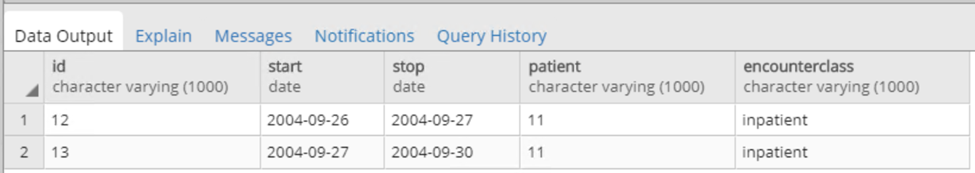
\includegraphics[width=1\linewidth]{images/ExtractTransformLoad/exerciseSourceData} 

}

\caption{Example source data.}\label{fig:exerciseSourceData}
\end{figure}

예시 답안은 Appendix \ref{Etlanswers}에서 확인할 수 있다.

\part{Data Analytics}\label{part-data-analytics}

\chapter{데이터 분석 이용 사례}\label{DataAnalyticsUseCases}

\emph{Chapter lead: David Madigan}

OHDSI는 실세계 헬스케어 데이터 (일반적으로 보험청구 또는 의무기록
데이터베이스)로부터 믿을만한 근거를 만들어내는데 초점을 맞춰 왔다.
OHDSI가 관심을 가져온 이용 사례들은 크게 3개의 카테고리로 구분된다:

\begin{itemize}
\tightlist
\item
  특성 분석
\item
  인구 수준 추정
\item
  환자 수준 예측
\end{itemize}

본 장에서는 각 카테고리들에 대해 설명한다. 모든 이용 사례들에 있어서,
생성된 근거들은 데이터 자체가 가지고 있는 한계를 이어 받는다는 점을
유념하라. 이 한계들에 대해서는 이 책의 ``근거의 질'' 챕터에서 다루고
있다. (챕터 \ref{EvidenceQuality} - \ref{MethodValidity})

\section{특성 분석}\label{-}

\index{characterization}

특성 분석은 다음과 같은 질문에 답변을 시도한다.

\begin{quote}
그들에게 무슨 일이 발생했는가?
\end{quote}

우리는 데이터를 이용하여 코호트 또는 전체 데이터베이스 내 환자들과
헬스케어의 특성을 묻는 질문에 답할 수 있으며, 시간이 경과함에 따라 이
특성들이 어떻게 변화하는지 알 수 있다.

데이터는 다음과 같은 질문들에 답을 제공할 수 있다:

\begin{itemize}
\tightlist
\item
  심방세동으로 새 진단을 받은 환자들 중 얼마나 많은 사람이 와파린을 처방
  받는가?
\item
  고관절 치환술을 받은 환자들의 평균 연령은 어떻게 되는가?
\item
  65세 이상 환자들 중 폐렴 발생률은 얼마나 되는가?
\end{itemize}

일반적인 특성 분석 질문들은 다음과 같이 표현된다:

\begin{itemize}
\tightlist
\item
  얼마나 많은 환자들이\ldots{}?
\item
  얼마나 자주\ldots{}?
\item
  환자들 중 어느 정도의 비율이\ldots{}?
\item
  \ldots{} 검사에 대한 결과값의 분포가 어떠한가?
\item
  \ldots{} 질병을 가진 환자들의 당화혈색소(HbA1c) 수준이 어떠한가?
\item
  \ldots{} 환자들에 대한 검사 결과값이 어떠한가?
\item
  환자가 \ldots{}에 노출되는 평균 노출 기간은 얼마인가?
\item
  \ldots{}의 시간 경과에 따른 트렌드는 무엇인가?
\item
  이 환자들이 사용하는 다른 약들이 무엇인가?
\item
  수반되는 치료법들이 무엇인가?
\item
  \ldots{}에 대한 충분한 케이스들이 있는가?
\item
  \ldots{}에 대한 연구X가 실행 가능한가?
\item
  \ldots{}에 대한 인구통계학적 특징은 무엇인가?
\item
  \ldots{}의 위험인자들이 무엇인가? (특정 위험인자가 구분된다면, 이는
  예측이 아닌 추정에 해당함)
\item
  \ldots{}의 예측요인들이 무엇인가?
\end{itemize}

그리고 원하는 결과값은 다음과 같다:

\begin{itemize}
\tightlist
\item
  건수 또는 퍼센트
\item
  평균
\item
  기술 통계값
\item
  발병률
\item
  유병율
\item
  코호트
\item
  규칙 기반 표현형
\item
  약물 사용
\item
  질병의 자연 경과
\item
  이행
\item
  동반질환 프로필
\item
  치료 경로
\item
  치료 요법
\end{itemize}

\section{인구 수준 추정}\label{--}

\index{population-level estimation}

데이터가 한정된 범위까지는 헬스케어 개입의 효과에 대한 인과적 추론들을
제공할 수 있다

\begin{quote}
무엇이 인과 효과들인가?
\end{quote}

우리는 행동의 결과를 이해하기 위해 인과 효과를 파악하고자 한다. 예를
들어, 우리가 어떤 치료법을 사용하기로 결정했다면, 이것이 앞으로 우리에게
무슨 변화를 일으킬까?

데이터는 다음과 같은 질문들에 답을 줄 수 있다:

\begin{itemize}
\tightlist
\item
  새로 심방세동으로 진단받은 환자들에 있어서, 치료 시작한지 1년 내에
  와파린이 다비가트란보다 주요 출혈을 더 일으키는가?
\item
  메트포르민이 설사에 미치는 인과 효과가 연령에 따라 다른가?
\end{itemize}

일반적인 인구 수준 효과 추정 질문들은 다음과 같이 표현된다:

\begin{itemize}
\tightlist
\item
  \ldots{}의 효과는 무엇인가?
\item
  내가 개입한다면 어떻게 될까\ldots{}?
\item
  어떤 치료가 더 효과가 좋을까?
\item
  X가 Y에 미치는 위험이 무엇일까?
\item
  \ldots{} 이벤트 발생에 걸리는 시간이 얼마나 될까?
\end{itemize}

그리고 원하는 결과값은 다음과 같다:

\begin{itemize}
\tightlist
\item
  상대 위험도
\item
  발생 위험비
\item
  승산비
\item
  평균 처치 효과
\item
  인과 관계
\item
  연관 관계
\item
  상관 관계
\item
  안전성 감시
\item
  비교 효과
\end{itemize}

\section{환자 수준 예측}\label{--}

\index{patient-level prediction}

데이터베이스에 쌓인 환자 건강 이력을 기반으로, 우리는 미래에 발생할 건강
이벤트에 대해 환자 수준의 예측을 할 수 있다.

\begin{quote}
나에게 무슨 일이 발생할까?
\end{quote}

데이터는 다음과 같은 질문에 답을 제공할 수 있다:

\begin{itemize}
\tightlist
\item
  주요 우울증으로 새롭게 진단 받은 특정 환자가 진단받은지 1년 안에
  자살을 시도할 확률이 얼마나 되는가?
\item
  심방세동으로 새롭게 진단 받은 특정 환자가, 와파린으로 치료를 시작한지
  1년 안에 허혈성 뇌졸증을 겪을 확률이 얼마나 되는가?
\end{itemize}

일반적인 환자 수준 예측에 대한 질문들은 다음과 같이 표현된다:

\begin{itemize}
\tightlist
\item
  이 환자가 \ldots{}할 가능성이 얼마나 되는가?
\item
  \ldots{}에 대한 후보자들이 누구인가?
\end{itemize}

그리고 원하는 결과값은 다음과 같다:

\begin{itemize}
\tightlist
\item
  개인에 대한 확률
\item
  예측 모델
\item
  높은/낮은 위험군
\item
  확률론적 표현형
\end{itemize}

인구 수준 추정과 환자 수준 예측은 어느 정도 중복된다. 예를 들어, 예측을
위한 중요한 이용사례는 특정 환자의 결과에 약물 A가 처방되었다고 예측하고
약물 B가 처방된 것과 동일한 결과가 나타나는지 예측하는 것이다. 실제로 이
약들 중 하나(약물 A이라고 하자)를 처방 받았고, 약물 A의 예상되는 결과가
실제로 일어나는지를 살펴봤다고 가정해 보자. 약물 B는 처방되지 않았고
치료 B 이후의 결과는 관찰된 적이 없으므로 예측은 할 수 있더라도 사실과
다를 수 있다. 이러한 각각의 예측 작업은 환자 수준 예측에 속한다. 그러나
두 결과의 차이(또는 비율)는 단위 수준의 \emph{인과적} 효과이며, 인과적
영향 추정 방법을 사용하여 추정해야 한다.

\BeginKnitrBlock{rmdimportant}
사람들은 예측모델을 인과모델로 잘못 해석하는 자연스러운 경향이 있다.
그러나 예측 모델은 인과성이 아닌 상관성만을 보여줄 수 있다. 예를 들자면,
당뇨병이 심근경색의 강한 예측변수이기 때문에, 당뇨병 약의 사용이
심근경색의 강한 예측변수일 수 있다. 그러나 이것이 당뇨병 약 복용을
중단하는 것이 심근경색을 막는다는 것을 의미하는 것은 아니다!
\EndKnitrBlock{rmdimportant}

\section{고혈압 이용 사례 예}\label{---}

당신은 고혈압의 1차 요법으로서 ACE 억제제 단일요법과 타이아자이드 이뇨제
단일요법이 급성 심근경색과 혈관부종에 미치는 영향을 연구하는데 관심이
있는 연구자이다. 당신은 OHDSI 연구에 기반하여 인구 수준 추정 연구질문을
도출했지만, 먼저 관심을 가지고 있는 특정 치료에 대한 특성을 어떻게
분석할 것인지 해결해야 한다.

\subsection{특성 분석 질문}\label{--}

급성 심근경색은 고혈압 환자들에게 일어날 수 있는 심혈관계 합병증으로,
고혈압에 대한 효과적인 치료로 이 위험을 줄여야 한다. 혈관부종은
희귀하지만 잠재적으로 심각한 ACE 억제제의 알려진 부작용이다. 당신은 관심
약제(ACE 억제제와 타이아자이드 이뇨제)들에 노출된 코호트 (챕터
\ref{Cohorts} 참고) 들을 생성하는 것으로부터 연구를 시작한다. 노출된
환자들의 인구통계학적 정보, 병적 상태, 병용 약물 등 기저 특성을 파악하기
위하여 특성 분석 (챕터 \ref{Characterization} 참고) 을 수행한다. 또한 이
노출 환자 내에서 분석하고자 하는 결과가 얼마나 발생하는지 추정하는 또
다른 특성 분석을 수행한다. 그리고, 당신은 `얼마나 자주 1) 급성
심근경색과 2) 혈관부종이 ACE 억제제와 타이아자이드 이뇨제에 노출된 기간
동안 발생하는가?'를 묻게 된다. 이러한 특성 분석은 인구 수준 추정 연구
수행의 실현 가능성을 판단하게 하고, 두 치료군이 비교 가능한지를 평가하게
하며, 환자들이 받는 치료에 예측되는 위험 요소들을 파악할 수 있게 한다.

\subsection{인구 수준 추정 질문}\label{---}

인구 수준 효과 추정 연구 (챕터 \ref{PopulationLevelEstimation} 참고) 는
ACE 억제제와 타이아자이드 이뇨제가 급성 심근경색과 혈관부종에 미치는
상대 위험을 추정한다. 더 나아가, 진료군과 음성대조군 분석을 통해 평균
치료 효과에 대해 믿을 수 있는 추정치를 도출했는지 평가한다.

\subsection{환자 수준 예측 질문}\label{---}

당신은 노출의 인과적 영향 여부와 상관없이, 가장 위험한 결과에 처한
환자들을 알아내고자 할 수 있다. 이것은 환자 수준 예측 (챕터
\ref{PatientLevelPrediction} 참고) 의 문제이다. ACE 억제제를 처음
사용하는 환자들 중 치료 시작한지 1년 동안 급성 심근경색 발병 위험이 가장
높은 환자들을 평가하는 예측 모델을 개발한다고 생각해 보아라. 이 모델을
통해 우리는 처음으로 ACE 처방을 받은 환자의 병력에서 관찰된 사건을
바탕으로, 향후 1년 동안 급성 심근경색을 겪을 가능성을 예측할 수 있다.

\section{관찰 연구의 한계}\label{--}

\index{limitations of obervational research}

OHDSI 데이터베이스가 답변을 제공할 수 없는 중요한 헬스케어 질문들이 많이
존재한다. 아래 질문들이 이에 해당한다:

\begin{itemize}
\tightlist
\item
  위약과 비교한 치료의 인과 효과. 때때로 치료의 인과 효과를 위약 치료가
  아닌 비치료와 비교하여 분석하는 것은 가능하다.
\item
  처방전 없이 구입할 수 있는 의약품과 관련된 모든 것
\item
  많은 결과와 다른 변수들이 거의 기록되지 않음. 사망률, 행동 결과,
  라이프 스타일 및 사회-경제적 지위와 같은 것들이 이에 포함된다.
\item
  환자는 건강이 좋지 않을 때만 의료 시스템을 이용하는 경향이 있기
  때문에, 치료의 이점을 측정하는 것이 쉽지 않다.
\end{itemize}

\subsection{잘못된 데이터}\label{-}

OHDSI 데이터베이스에 기록된 임상 데이터는 의료 현실과 차이가 있을 수
있다. 예를 들어, 환자가 심근 경색을 경험한 적이 없어도 환자의 기록에
심근 경색 코드가 포함되어 있을 수 있다. 마찬가지로 검사 값이
잘못되었거나 시술에 대한 잘못된 코드가 데이터베이스에 저장되었을 수도
있다. \ref{DataQuality}와 \ref{ClinicalValidity} 챕터는 이와 같은
이슈들을 다루고 있으며, 모범 사례를 통해 이러한 문제들을 최대한 식별하고
수정하고자 한다. 그럼에도 불구하고, 잘못된 데이터는 필연적으로 어느
정도까지 존재할 수 밖에 없으며, 분석의 타당성을 약화시킬 수 있다. 매우
많은 문헌들이 데이터 오류들을 처리하기 위한 통계적 추론 조정에 초점을
맞추고 있다. - 예: \citet{fuller2009measurement} 참조

\subsection{결측 데이터}\label{-}

\index{missing data}

OHDSI 데이터베이스에서의 결측은 감지하기 어려운 문제점들을 낳는다.
데이터베이스에 기록되어야 하는 건강 이벤트(예: 처방, 검사 값 등)가
기록되지 않은 것, 그것이 ``결측''이다. 통계 문헌들은 ``임의의 완전
결측'', ``임의의 결측'', ``임의가 아닌 결측''과 같은 결측 유형들과
이러한 유형들을 다루는 복잡한 방법론들을 구별하고 있다.
\citet{perkins2017principled} 가 이 주제에 대한 유용한 입문서를
제공한다.

\section{요약}\label{-3}

\BeginKnitrBlock{rmdsummary}
\begin{itemize}
\item
  관찰 연구의 이용 사례들은 크게 3개의 카테고리로 구분된다.
\item
  \textbf{특성 분석}은 ``그들에게 무슨 일이 발생했는가?''라는 질문에
  답하는 것을 목적으로 한다.
\item
  \textbf{인구 수준 추정}은 ``인과적 영향이 무엇인가?''라는 질문에
  답하는 것을 목적으로 한다.
\item
  \textbf{환자 수준 예측}은 ``나에게 무엇이 일어날까?''라는 질문에
  답하는 것을 목적으로 한다.
\item
  예측 모델은 인과 모델이 아니다; 강한 예측변수에 대한 개입이 결과에
  영향을 미칠 것이라고 믿을 근거가 없다.
\item
  헬스케어 관찰 데이터를 이용하여 연구할 수 없는 질문들도 있다.
\end{itemize}
\EndKnitrBlock{rmdsummary}

\section{연습문제}

\BeginKnitrBlock{exercise}
\protect\hypertarget{exr:exerciseUseCases1}{}{\label{exr:exerciseUseCases1}
}다음 질문들은 어떤 사용 사례 카테고리에 해당하는가?

\begin{enumerate}
\def\labelenumi{\arabic{enumi}.}
\item
  비스테로이드 약물에 최근 노출되었던 환자들이 위장관 출혈을 겪을 비율을
  계산하라.
\item
  기저 특성을 기반으로 특정 환자가 차년도에 위장관 출혈을 겪을 확률을
  계산하라.
\item
  셀레콕시브와 비교하여 디클로페낙이 위장관 출혈에 미치는 위험을
  추정하라.
\end{enumerate}
\EndKnitrBlock{exercise}

\BeginKnitrBlock{exercise}
\protect\hypertarget{exr:exerciseUseCases2}{}{\label{exr:exerciseUseCases2}
}당신은 디클로페낙이 위장관 출혈에 미치는 위험을 비노출(위약)의 경우와
비교하여 추정하고자 한다. 이와 같은 연구가 헬스케어 관찰 데이터를
이용하여 수행 가능한가?
\EndKnitrBlock{exercise}

정답은 부록 \ref{UseCasesanswers}에서 확인할 수 있다.

\chapter{OHDSI Analytics Tools}\label{OhdsiAnalyticsTools}

\emph{Chapter leads: Martijn Schuemie \& Frank DeFalco}

OHDSI는 관찰 환자 수준 데이터에 대한 다양한 데이터 분석 사용 사례를
지원하는 광범위한 오픈 소스 도구를 제공한다. 이러한 도구의 공통점은 공통
데이터 모델(CDM)을 사용하여 하나 이상의 데이터베이스와 상호 작용할 수
있다는 것이다. 또한, 이러한 도구는 다양한 사용 사례에 대한 분석을
표준화한다. 처음부터 시작하는 것이 아니라 표준 템플릿을 작성함으로써
분석을 구현할 수 있다. 이렇게 하면 분석을 더 쉽게 수행할 수 있고,
재현성과 투명성을 향상시킬 수 있다. 예를 들어, 발생률을 계산하는 방법은
무한에 가까운 수가 있는 것처럼 보이지만, 이러한 방법은 몇 가지
선택사항으로 OHDSI 도구에 지정할 수 있으며, 동일한 선택을 하는 사람은
동일한 방법으로 발병률을 계산할 것이다.

이 장에서는 먼저 분석을 실행하기 위해 선택할 수 있는 다양한 방법과
분석에서 어떤 전략을 사용할 수 있는지 설명한다. 그런 다음 다양한 OHDSI
툴과 다양한 사용 사례에 적합한 방법을 검토한다.

\section{Analysis Implementation}\label{analysisImplementation}

그림 \ref{fig:implementations} 은 CDM을 사용하여 데이터베이스에 대한
연구를 구현하도록 선택할 수 있는 다양한 방법을 보여준다.
\index{analysis implementation}

\begin{figure}

{\centering 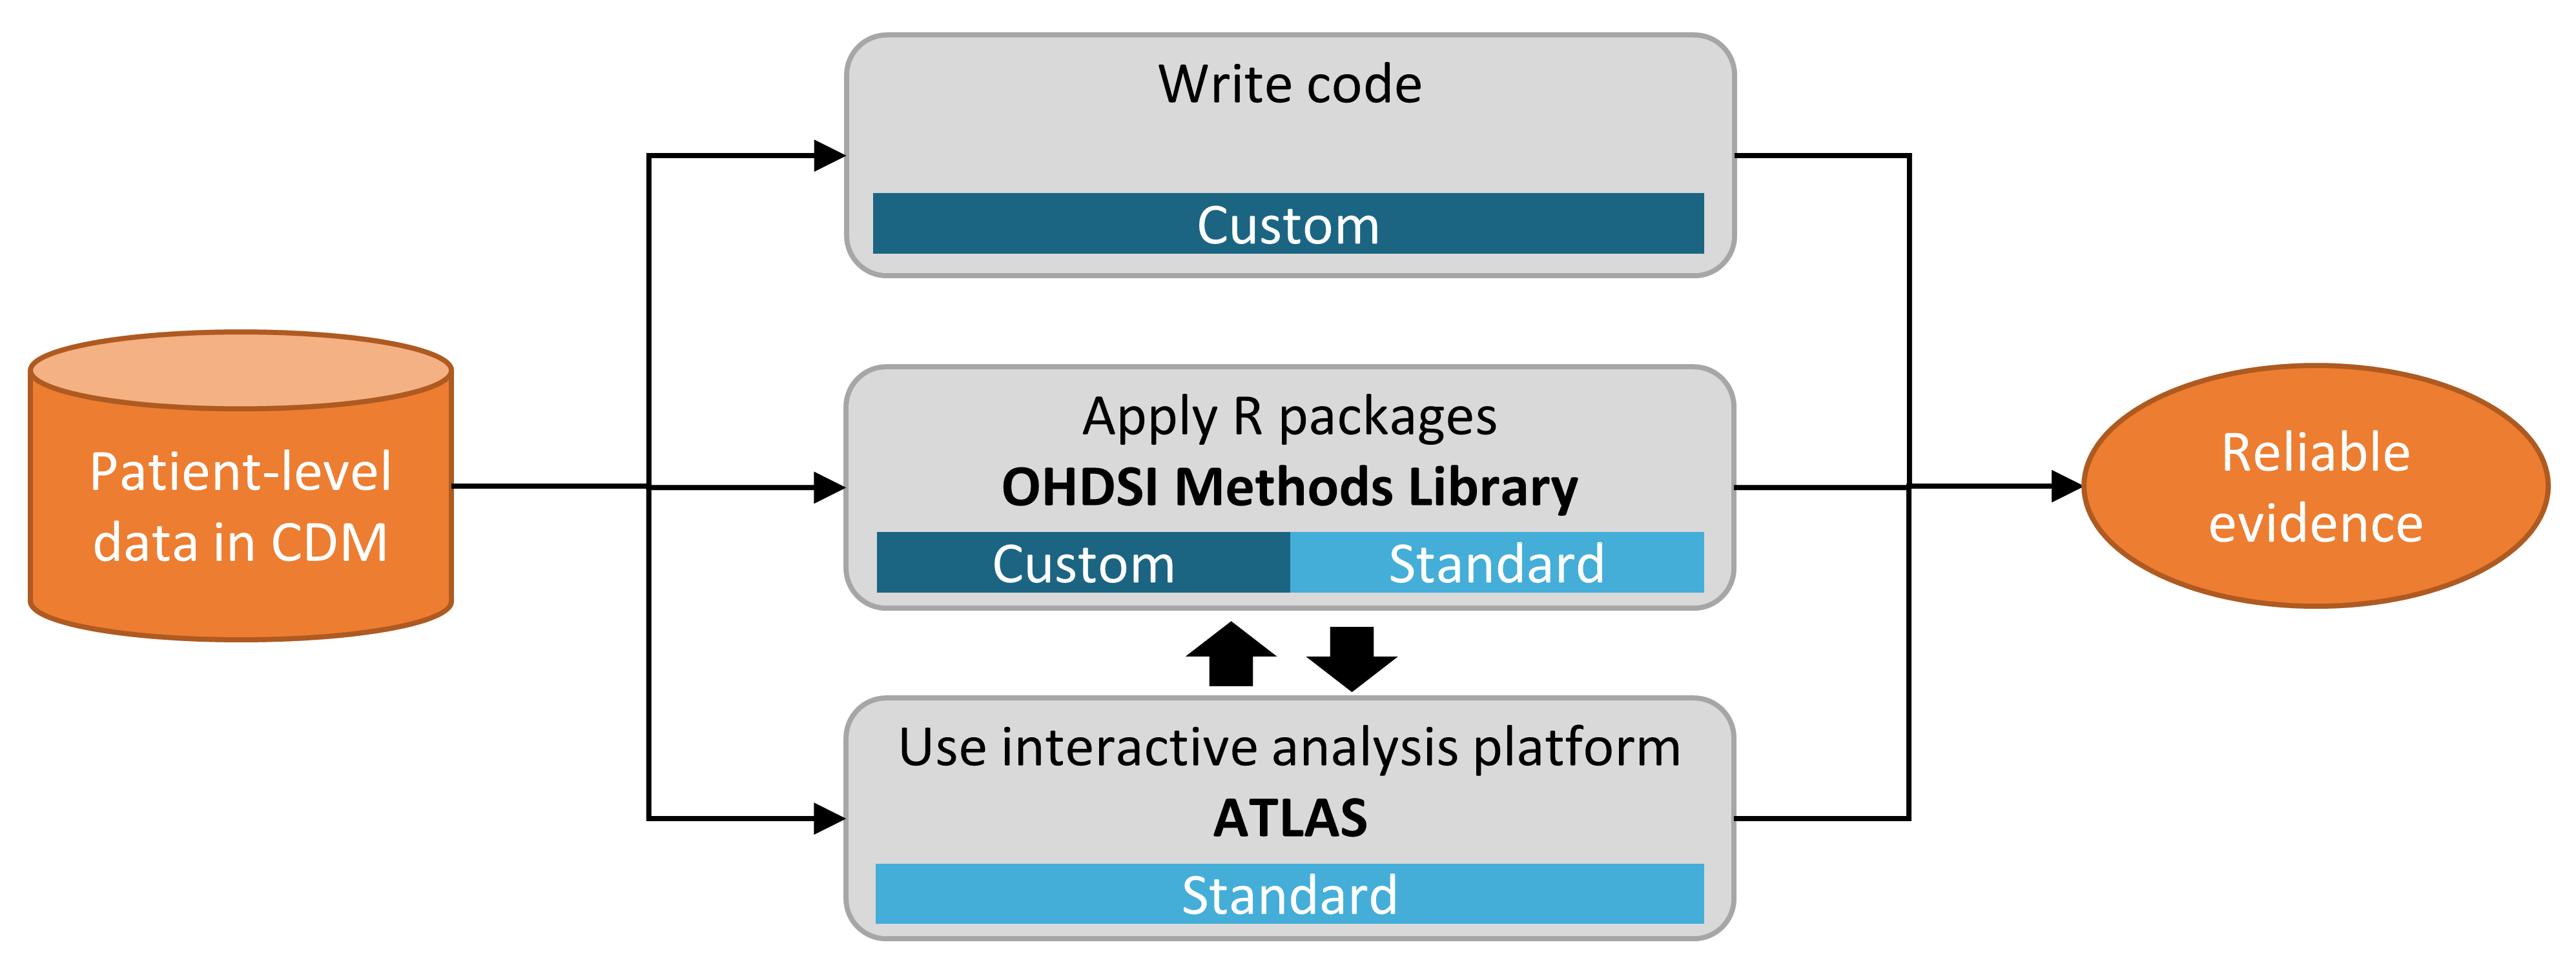
\includegraphics[width=0.9\linewidth]{images/OhdsiAnalyticsTools/implementations} 

}

\caption{CDM의 데이터에 대한 분석을 구현하는 다양한 방법}\label{fig:implementations}
\end{figure}

연구를 이행하는 데는 세 가지 주요 접근법이 있다. 첫 번째는 OHDSI가
제공해야 하는 도구를 사용하지 않는 사용자 정의 코드를 작성하는 것이다.
R, SAS 또는 다른 언어로 de novo 분석을 쓸 수 있다. 이는 최대의 유연성을
제공하며, 특정 분석이 우리의 툴에 의해 뒷받침되지 않는 경우 사실상
유일한 선택사항이 될 수 있다. 그러나 이러한 경로에는 많은 기술적 스킬과
시간, 노력이 필요하며, 분석이 복잡성이 증가함에 따라 코드의 오류를
피하기 어려워진다.

두 번째 접근방식은 R의 분석 개발과
\href{https://ohdsi.github.io/MethodsLibrary/}{OHDSI Methods Library}의
패키지 사용을 포함한다. 최소한 \ref{SqlAndR}장에 설명되어 있는
\href{https://ohdsi.github.io/SqlRender/}{SqlRender} 및
\href{https://ohdsi.github.io/DatabaseConnector/}{DatabaseConnector}
패키지를 사용하여 PostgreSQL, SQL Server, 그리고 Oracle과 같은 다양한
데이터베이스 플랫폼에서 동일한 코드를 실행할 수 있다.
\href{https://ohdsi.github.io/CohortMethod/}{CohortMethod}와
\href{https://ohdsi.github.io/PatientLevelPrediction/}{PatientLevelPrediction}과
같은 다른 패키지는 자신의 코드로 호출할 수 있는 CDM에 대한 고급 분석을
위한 R 기능을 제공한다. 이것은 여전히 많은 기술적 전문지식을 필요로
하지만, Methods Library의 검증된 구성요소를 다시 사용함으로써 우리는
완전한 사용자 정의 코드를 사용할 때보다 더 효율적이고 오류가 덜 발생할
수 있다.

세 번째 접근법은 프로그래머가 아닌 사람들이 다양한 분석을 효율적으로
수행할 수 있도록 해주는 웹 기반 툴인 우리의 대화형 분석 플랫폼
\href{https://github.com/OHDSI/Atlas/wiki}{ATLAS}에 의존한다. ATLAS는
Method Libraries를 사용하지만 분석을 설계하기 위한 간단한 그래픽
인터페이스를 제공하며 많은 경우 분석을 실행하는 데 필요한 R 코드를
생성한다. 그러나 ATLAS는 Methods Library에서 사용할 수 있는 모든 옵션을
지원하지 않는다. 대부분의 연구가 ATLAS를 통해 수행될 수 있을 것으로
예상되지만, 일부 연구는 두 번째 접근방식이 제공하는 유연성을 요구할 수
있다.

ATLAS와 Methods Library는 독립적이지 않다. ATLAS에서 호출할 수 있는 더
복잡한 분석 중 일부는 Methods Library의 패키지에 대한 호출을 통해
실행된다. 마찬가지로 Methods Library에 사용되는 코호트는 ATLAS에서
설계되는 경우가 많다.

\section{Analysis Strategies}\label{analysis-strategies}

사용자 정의 코드를 사용하거나 Methods Library의 표준 분석 코드를
사용하여 CDM에 대한 분석을 구현하는 것 외에도, 그러한 분석 기법을
사용하여 근거를 생성하는 데에는 여러 가지 전략이 있다. 그림
\ref{fig:strategies}는 OHDSI에 채택된 세 가지 전략을 강조한다.

\begin{figure}

{\centering 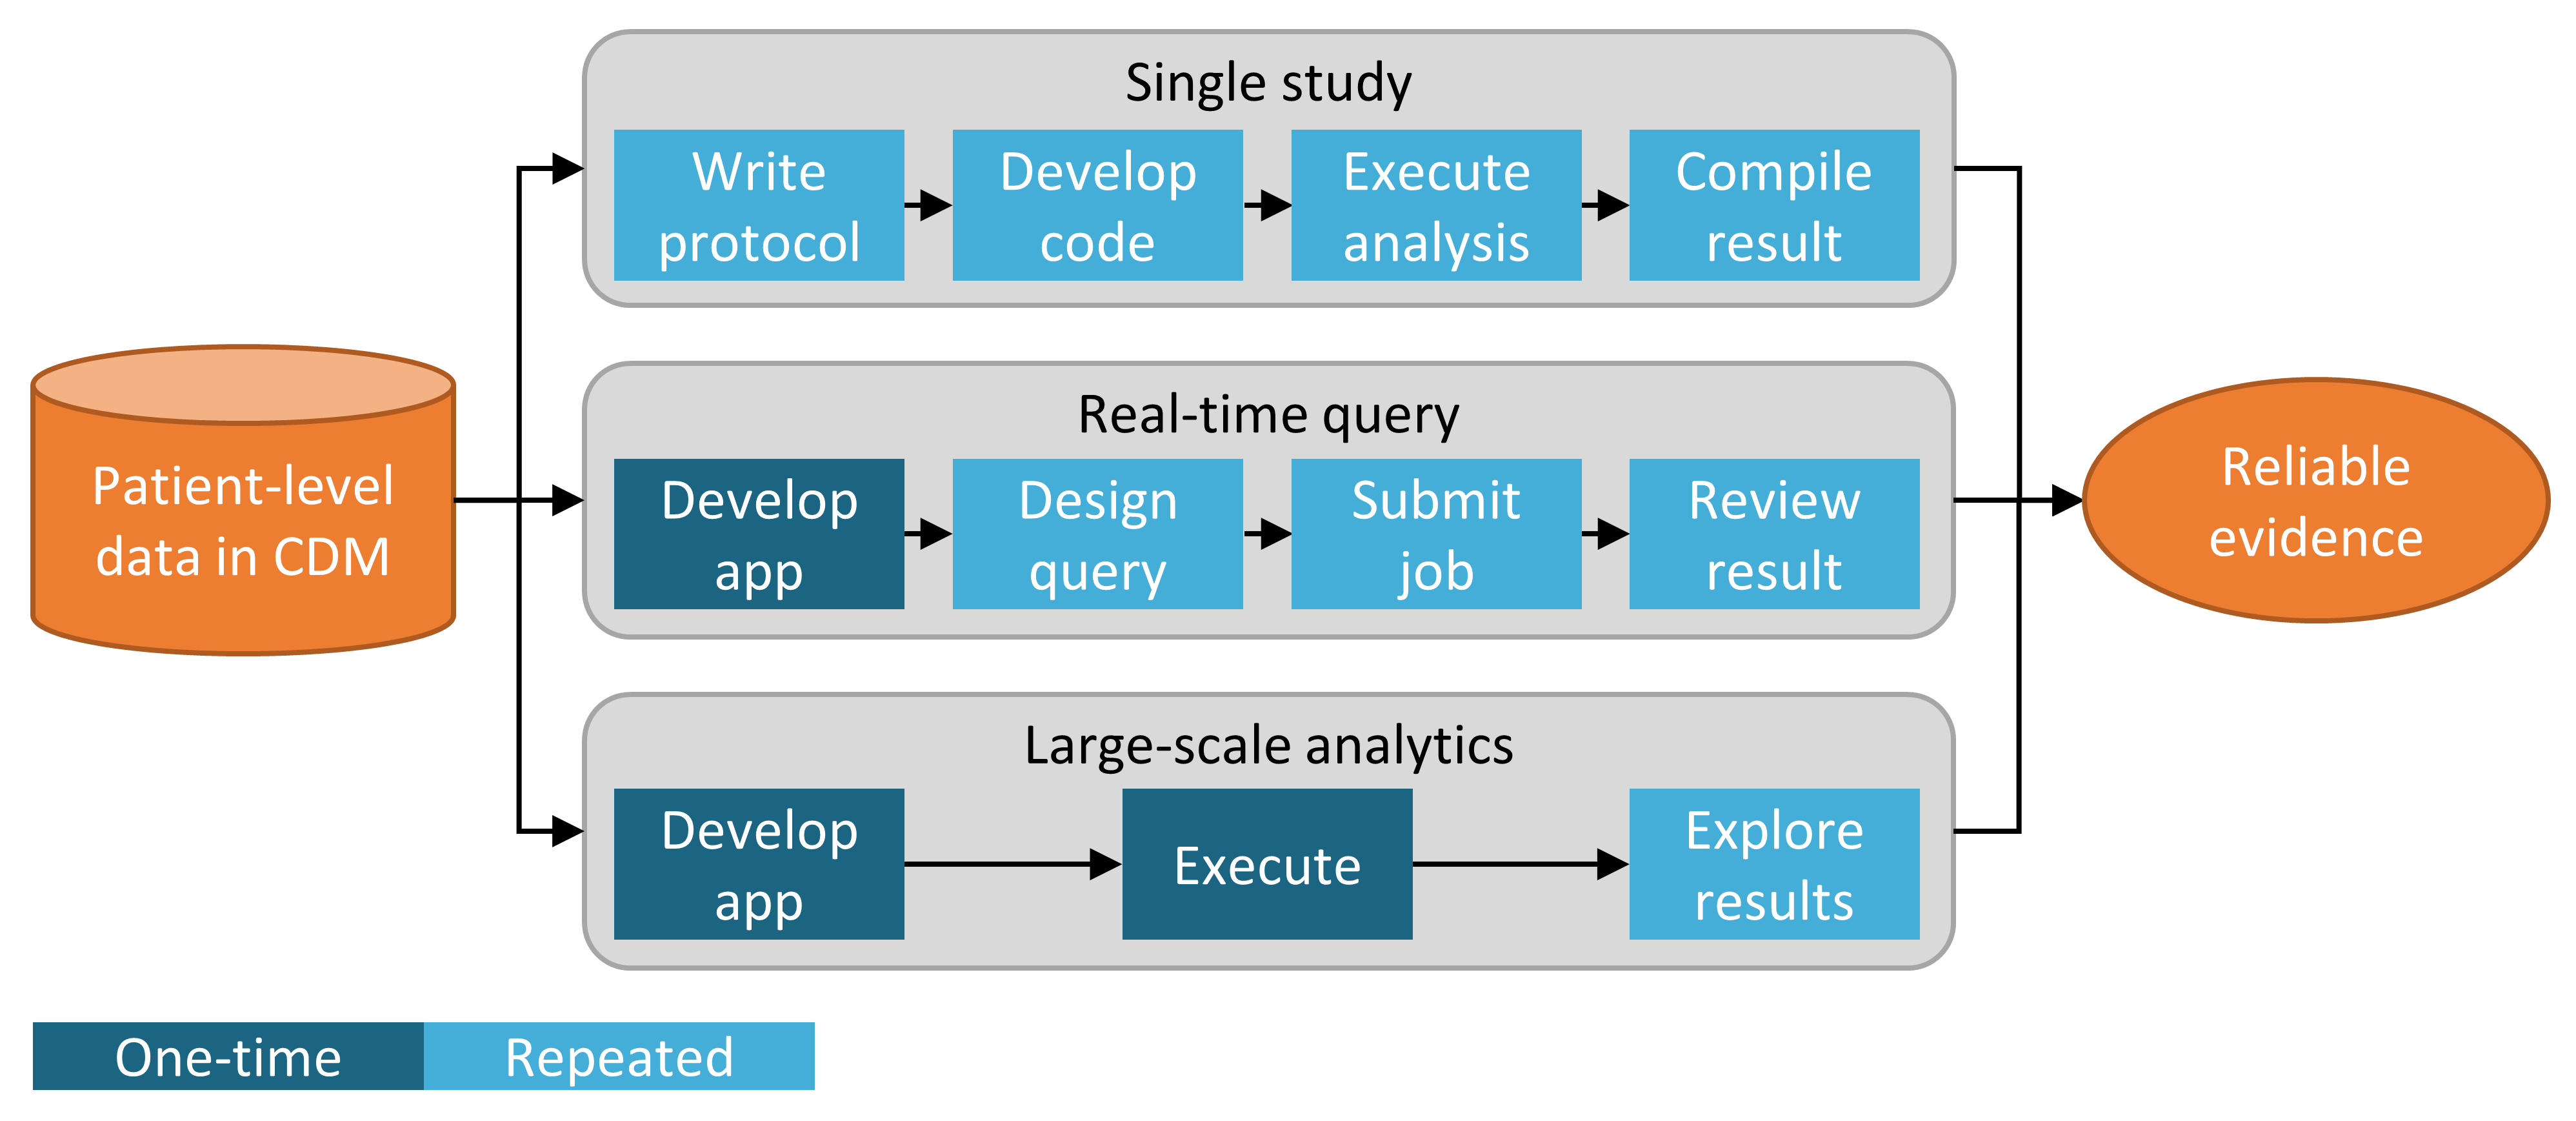
\includegraphics[width=0.9\linewidth]{images/OhdsiAnalyticsTools/strategies} 

}

\caption{(임상적) 질문에 대한 근거를 생성하기 위한 전략}\label{fig:strategies}
\end{figure}

첫 번째 전략은 모든 분석을 하나의 개별적인 연구로 본다. 분석은
프로토콜에 미리 지정되어야 하고, 코드로 구현되어야 하며, 데이터에 대해
실행되어야 하며, 그 후에 결과를 컴파일하고 해석할 수 있어야 한다. 모든
질문에 대해 모든 단계를 반복해야 한다. 그러한 분석의 예로는 phenytoin과
비교하여 levetiracetam과 관련된 혈관부종(angioedema)의 위험에 대한 OHDSI
연구가 있다. \citep{duke_2017} 이 연구에서, 프로토콜이 처음으로
작성되었고, OHDSI Methods Library를 이용한 분석 코드가 OHDSI 네트워크를
통해 개발되어 실행되었으며, 결과를 편집하여 저널 간행물에 배포하였다.

두 번째 전략은 사용자가 특정 종류의 질문에 실시간으로 또는 거의
실시간으로 답할 수 있는 애플리케이션을 개발한다. 애플리케이션이 개발되면
사용자는 상호 작용적으로 쿼리를 정의하고 제출하고 결과를 볼 수 있다. 이
전략의 예로는 ATLAS의 코호트 정의 및 생성 도구가 있다. 이 도구는
사용자가 다양한 복잡성에 대한 코호트 정의를 지정하고, 다양한 포함 및
제외 기준을 충족하는 사용자 수를 확인하기 위해 데이터베이스에 대한
정의를 실행할 수 있도록 한다.

세 번째 전략은 비슷하게 질문의 종류에 초점을 맞추지만, 그 다음 클래스
내의 질문에 대한 모든 근거를 남김없이 생성하려고 시도한다. 사용자는
다양한 인터페이스를 통해 필요에 따라 근거를 탐색할 수 있다. 한 예로
우울증 치료의 영향에 대한 OHDSI 연구가 있다. \citep{schuemie_2018b} 이
연구에서 모든 우울증 치료는 4개의 큰 관찰 데이터베이스에서 관심 있는 큰
결과 집합에 대해 비교된다. 광범위한 연구 진단과 함께 경험적으로 보정된
위험 비율 17,718을 포함한 전체 결과는 대화형 웹 앱에서 이용할 수
있다.\footnote{\url{http://data.ohdsi.org/SystematicEvidence/}}

\section{ATLAS}\label{atlas}

ATLAS는 CDM 형식으로 표준화된 환자 수준 관측 데이터에 대한 분석의 설계와
실행을 촉진하는 OHDSI 커뮤니티에서 개발한 무료 웹 기반 툴이다. ATLAS는
OHDSI WebAPI와 함께 웹 애플리케이션으로 배포되며 일반적으로 Apache
Tomcat에서 호스팅된다. 실시간 분석을 수행하려면 CDM에 있는 환자 수준
데이터에 액세스해야 하므로 일반적으로 조직의 방화벽 뒤에 설치된다.
그러나 공용 ATLAS\footnote{\url{http://www.ohdsi.org/web/atlas}}도
있으며, 이 ATLAS 인스턴스는 몇 개의 소규모 시뮬레이션 데이터셋에만
액세스할 수 있지만, 여전히 테스트와 훈련을 포함한 여러 용도로 사용할 수
있다. ATLAS의 공개 인스턴스를 사용하여 효과 추정 또는 예측 연구를 완전히
정의하고, 연구를 실행하기 위한 R 코드를 자동으로 생성할 수도 있다. 이
코드는 ATLAS와 WebAPI를 설치할 필요 없이 사용 가능한 CDM이 있는 모든
환경에서 실행될 수 있다. \index{ATLAS}

\begin{figure}

{\centering 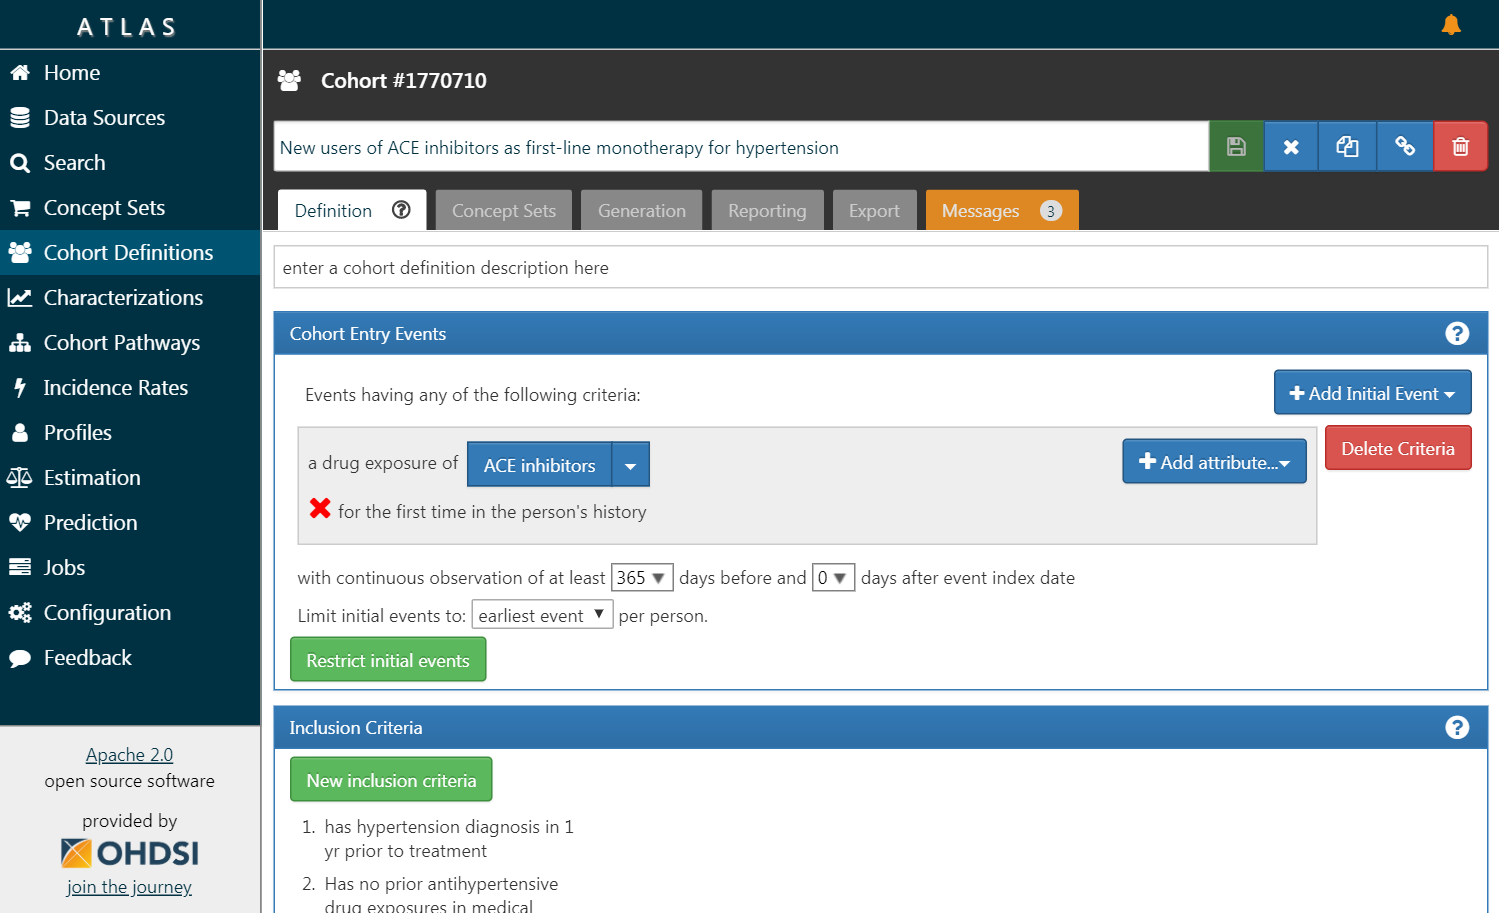
\includegraphics[width=1\linewidth]{images/OhdsiAnalyticsTools/atlas} 

}

\caption{ATLAS 사용자 인터페이스}\label{fig:atlas}
\end{figure}

ATLAS 스크린샷은 그림 \ref{fig:atlas} 에 제공된다. 왼쪽에는 ATLAS에서
제공하는 다양한 기능을 보여주는 내비게이션 바가 있다:

\begin{description}
\tightlist
\item[Data Sources \index{ATLAS!Data Sources}
\index{Achilles|see {ATLAS!data sources}}]
데이터 원본(Data sources)은 Atlas 플랫폼 내에서 구성한 각 데이터 원본에
대해 기술적이고 표준화된 보고 기능을 제공한다. 이 기능은 대규모 분석
전략을 사용한다. 모든 서술은 사전에 계산된 것이다. 데이터 출처는
\ref{Characterization}장에서 논한다.
\item[Vocabulary Search \index{ATLAS!vocabulary search}]
Atlas는 OMOP 표준화된 어휘를 검색하고 탐색하여 그러한 어휘 안에 존재하는
개념과 데이터 소스에 대한 표준화된 분석에서 그러한 개념을 적용하는
방법을 이해할 수 있는 능력을 제공한다. 이 특성은
\ref{StandardizedVocabularies}장에서 논한다.
\item[Concept Sets \index{ATLAS!concept sets}]
개념 집합은 표준화된 분석에서 사용할 개념 집합을 식별하는 데 사용할 수
있는 논리 표현식의 집합을 만들 수 있는 능력을 제공한다. 개념 집합은
단순한 코드나 값 리스트보다 더 정교하게 만들어 준다. 개념 집합은
사용자가 어휘 계층에 관련 개념을 포함하거나 배제하는 것에 관심이 있다는
것을 명시할 수 있도록 하는 논리적 지표와 함께 표준화된 어휘에서 나온
여러 개념으로 구성되어 있다. 어휘를 검색하고, 개념 집합을 식별하며, 개념
집합을 해결하기 위해 사용할 논리를 명시하는 것은 분석 계획에 자주
사용되는 모호한 의학 언어를 정의하는 강력한 메커니즘을 제공한다. 이러한
개념 집합은 ATLAS 내에 저장한 다음 코호트 정의 또는 분석 규격의 일부로
분석 내내 사용할 수 있다.
\item[Cohort Definitions \index{ATLAS!cohort definitions}]
코호트 정의는 일정 기간 동안 하나 이상의 기준을 충족하는 일련의 사람들을
구성할 수 있는 능력이며, 이러한 코호트는 이후 모든 분석에 대한 입력의
기초가 될 수 있다. 이 특성은 \ref{Cohorts}장에서 논한다.
\item[Characterizations \index{ATLAS!cohort characterization}]
특성은 당신이 정의한 하나 이상의 코호트를 보고 그 환자군에 대한 특성을
요약할 수 있는 분석 능력이다. 이 기능은 실시간 쿼리 전략을 사용하며,
\ref{Characterization}장에서 논한다.
\item[Cohort Pathways \index{ATLAS!cohort pathways}]
코호트 경로(Cohort pathways)는 하나 이상의 인구 내에서 발생하는 임상
사건의 순서를 살펴볼 수 있는 분석 툴이다. 이 기능은 실시간 쿼리 전략을
사용하며, \ref{Characterization}장에서 논한다.
\item[Incidence Rates \index{ATLAS!incidence rates}]
발생률은 관심 대상 인구 내에서 예후의 발생률을 추정할 수 있는 도구다. 이
기능은 실시간 쿼리 전략을 사용하며, \ref{Characterization}장에서 논한다.
\item[Profiles \index{ATLAS!profiles}]
프로필은 개별 환자에 대해 종적 관찰 데이터를 탐색하여 특정 개인 내에서
일어나는 일을 요약할 수 있는 도구다. 이 기능은 실시간 쿼리 전략을
사용한다.
\item[Population Level Estimation
\index{ATLAS!population level estimation}]
추정은 비교 코호트 설계를 사용하여 인구 수준 효과 추정 연구를 정의할 수
있는 능력이며, 여기서 하나 이상의 대상과 비교기 코호트 간의 비교를 통해
일련의 결과에 대해 탐색할 수 있다. 이 특징은 코딩이 필요하지 않으므로
실시간 쿼리 전략을 구현한다고 말할 수 있으며,
\ref{PopulationLevelEstimation}장에서 논의한다.
\item[Patient Level Prediction \index{ATLAS!patient level prediction}]
예측은 주어진 목표 노출 내에서 결과를 예측할 수 있는 환자 수준 예측
분석을 수행하기 위해 기계 학습 알고리즘을 적용할 수 있는 기능이다. 이
특성은 코딩이 필요하지 않으므로 실시간 쿼리 전략을 구현한다고 할 수
있으며, \ref{PatientLevelPrediction}장에서 논한다.
\item[Jobs \index{ATLAS!jobs}]
WebAPI를 통해 실행 중인 프로세스의 상태를 탐색하려면 작업 메뉴 항목을
선택하십시오. 작업은 종종 코호트 특성 보고서를 생성하거나 컴퓨팅 코호트
특성화 보고서를 생성하는 것과 같은 장기 실행 과정이다.
\item[Configuration \index{ATLAS!configuration}]
소스 구성 섹션에 구성된 데이터 소스를 검토하려면 구성 메뉴 항목을
선택하십시오.
\item[Feedback \index{ATLAS!feedback}]
피드백 링크는 Atlas의 이슈 로그로 이동시켜 새로운 이슈를 기록하거나 기존
이슈를 검색할 수 있도록 해준다. 새로운 기능이나 개선사항에 대한
아이디어가 있다면, 이것은 개발 커뮤니티에 대한 참고 사항이기도 하다.
\end{description}

\subsection{Security}\label{security}

ATLAS와 WebAPI는 전체 플랫폼 내의 기능 또는 데이터 소스에 대한 액세스를
제어하기 위한 세분화된 보안 모델을 제공한다. 이 보안 시스템은 Apache
Shiro 라이브러리를 활용하여 구축된다. 보안 시스템에 대한 추가 정보는
온라인 WebAPI 보안 위키에서 찾을 수 있다.\footnote{\url{https://github.com/OHDSI/WebAPI/wiki/Security-Configuration}}
\index{ATLAS!security}

\subsection{Documentation}\label{documentation}

ATLAS에 대한 설명서는 ATLAS GitHub repository wiki.\footnote{\url{https://github.com/OHDSI/ATLAS/wiki}}
이 위키에는 온라인 비디오 튜토리얼에 대한 링크뿐만 아니라 다양한
애플리케이션 기능에 대한 정보가 포함되어 있다.
\index{ATLAS!documentation}

\subsection{How to Install}\label{how-to-install}

ATLAS 설치는 OHDSI WebAPI와 함께 수행된다. 각 구성 요소의 설치 가이드는
ATLAS GitHub 저장소 설정 가이드\footnote{\url{https://github.com/OHDSI/Atlas/wiki/Atlas-Setup-Guide}}
및 WebAPI GitHub 저장소 설치 가이드\footnote{\url{https://github.com/OHDSI/WebAPI/wiki/WebAPI-Installation-Guide}}
\index{ATLAS!installation}

\section{Methods Library}\label{methods-library}

The \href{https://ohdsi.github.io/MethodsLibrary/}{OHDSI Methods
Library}는 그림 \ref{fig:methodsLibrary}에 표시된 오픈 소스 R 패키지의
모음입니다. \index{methods library}

\begin{figure}

{\centering 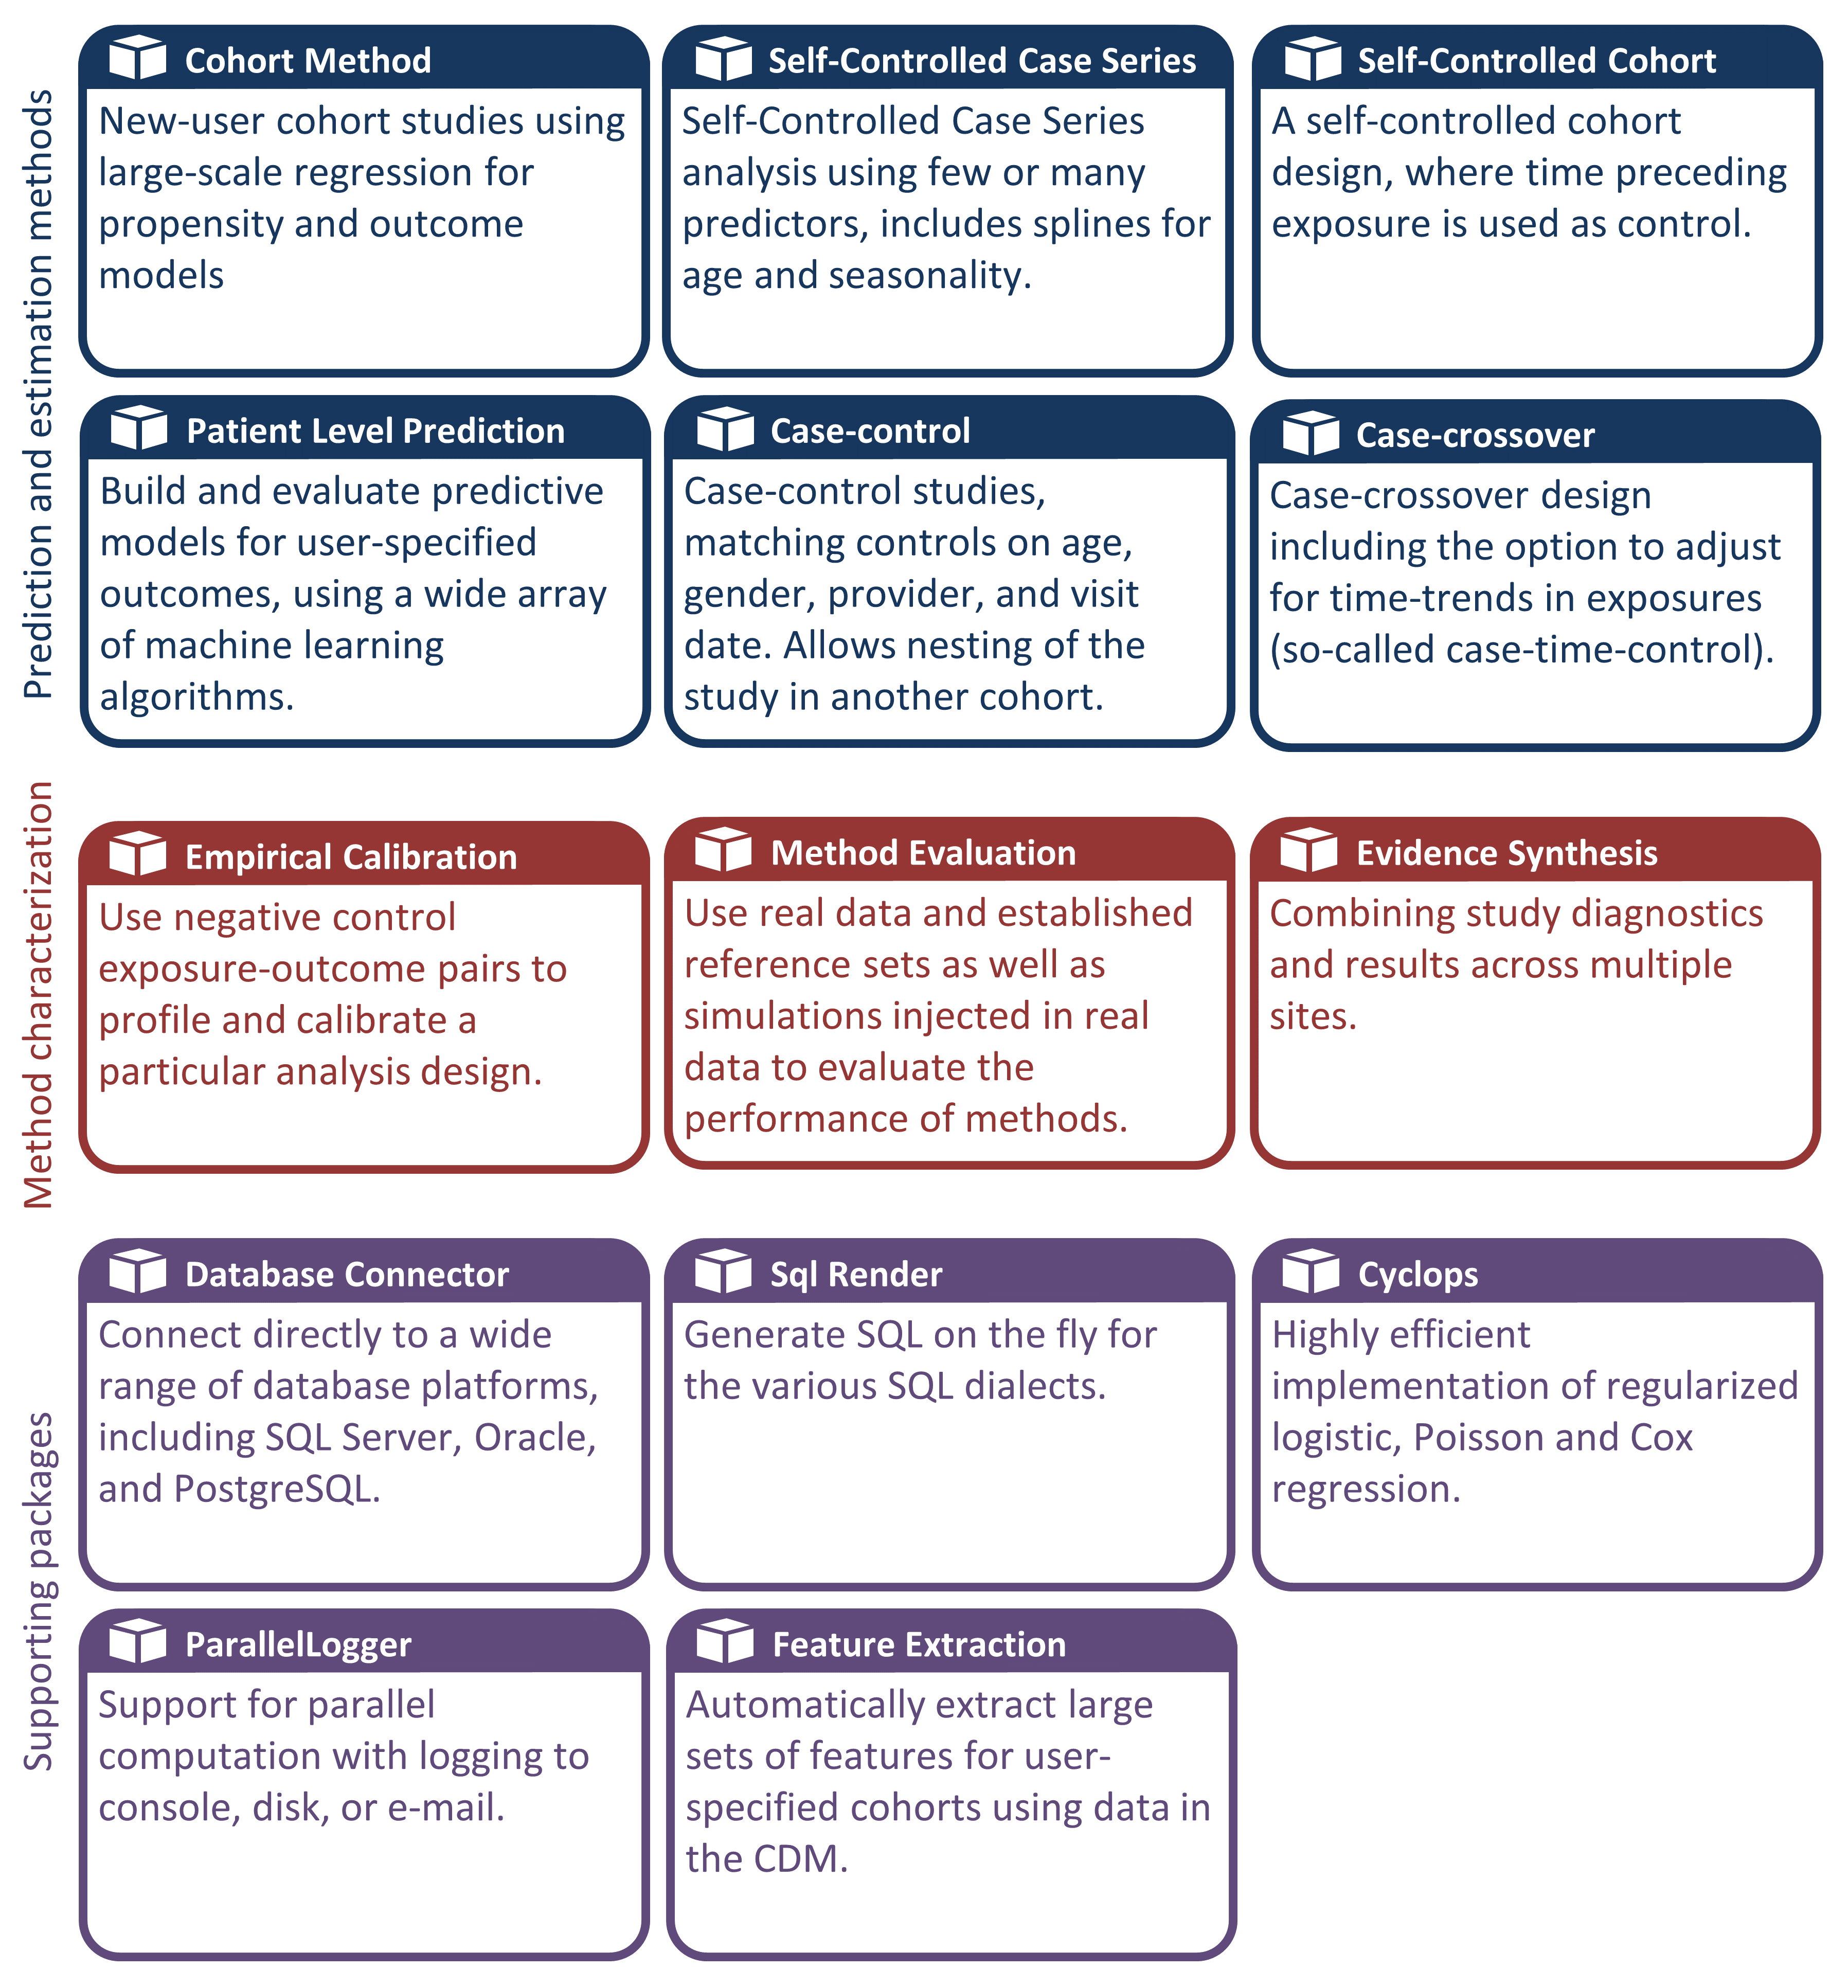
\includegraphics[width=1\linewidth]{images/OhdsiAnalyticsTools/methodsLibrary} 

}

\caption{The OHDSI Methods Library의 패키지}\label{fig:methodsLibrary}
\end{figure}

패키지는 완전한 관찰 연구를 수행하기 위해 함께 사용할 수 있는 R 기능을
제공하며, CDM의 데이터에서 시작하여 결과 추정치와 이를 뒷받침하는 통계,
수치 및 표를 제공한다. 패키지는 CDM의 관측 데이터와 직접 상호작용하며,
단순히 \ref{SqlAndR}장에서 설명한 대로 완전한 사용자 정의 분석에 대한
플랫폼 간 호환성을 제공하는 데 사용하거나, 인구 특성화를 위한 고급
표준화 분석(제 \ref{Characterization}장), 인구 수준 효과 추정(제
\ref{PopulationLevelEstimation}장) 및 환자 수준 예측(제
\ref{PatientLevelPrediction}장)을 제공할 수 있다. The Methods Library는
(이전 또는 진행 중인 연구에서 학습한) 투명성, 재현성, 뿐만 아니라 ``특정
맥락에서 methods의 작동 특성(operating characteristics) 측정'' 및
이어지는 ``methods로부터 생성된 측정치의 경험적 교정(empirical
calibration)''과 같은 관찰 데이터 및 관찰 연구 설계의 사용을 위한 모범
사례를 지원한다.

Method Library는 이미 발표된 많은 임상 연구
\citep{boland_2017, duke_2017, ramcharran_2017, weinstein_2017, wang_2017, ryan_2017, ryan_2018, vashisht_2018, yuan_2018, johnston_2019}와
방법론 연구에 사용되어 왔다.
\citep{schuemie_2014, schuemie_2016, reps2018, tian_2018, schuemie_2018, schuemie_2018b, reps_2019}
The Methods Library에서 방법 구현의 타당성은 \ref{SoftwareValidity}장에
설명되어 있다.

\subsection{Support for Large-Scale
Analytics}\label{support-for-large-scale-analytics}

모든 패키지에 통합된 한 가지 주요 특징은 많은 분석을 효율적으로 실행할
수 있는 능력이다. 예를 들어 인구 수준 추정을 수행할 때 CohortMethod
패키지는 다양한 분석 설정을 사용하여 많은 노출(exposure) 및
결과(outcome)에 대한 효과 크기 추정치(effect-size estimates)를 계산할 수
있도록 하며, 패키지는 필요한 모든 중간 및 최종 데이터 세트를 계산하는
최적의 방법을 자동으로 선택한다. ``공변량 추출(extraction of
covariates)''이나 하나의 대상 비교기 쌍(target-comparator pair)과 복수의
결과에 사용되는 ``성향 모델 장착(fitting a propensity model)''과 같이
재사용할 수 있는 단계는 한 번만 실행된다. 가능한 경우 계산 자원의 사용을
극대화하기 위해 연산은 병행으로 수행될 것이다.

이러한 계산 효율은 대규모 분석을 가능하게 하여 한꺼번에 많은 질문에 답할
수 있으며, 또한 제어 가설(예: 음성 제어(negative controls)을 포함시켜
우리 방법의 작동 특성(operating characteristics)을 측정하고
\ref{MethodValidity}장에 기술된 경험적 교정(empirical calibration)을
수행하는 데 필수적이다. \index{control hypotheses}

\subsection{Support for Big Data}\label{BigDataSupport}

The Methods Library는 또한 매우 큰 데이터베이스에 대해 실행하고 대량의
데이터를 포함하는 계산을 수행할 수 있도록 설계되었다. 이는 다음과 같은
세 가지 방법으로 달성되었다:

\begin{enumerate}
\def\labelenumi{\arabic{enumi}.}
\tightlist
\item
  대부분의 데이터 조작은 데이터베이스 서버에서 수행된다. 분석은
  일반적으로 데이터베이스에 있는 전체 데이터의 극히 일부만 필요로 하며
  Methods Library는 SqlRender 및 DatabaseConnector 패키지를 통해
  서버에서 고급 작업을 수행하여 관련 데이터를 사전 처리하고 추출할 수
  있도록 한다.
\item
  대용량 로컬 데이터 객체는 메모리 효율적인 방식으로 저장된다. 로컬
  시스템으로 다운로드 되는 데이터의 경우 Method Library는
  \href{https://cran.r-project.org/web/packages/ff}{ff} 패키지를
  사용하여 대용량 데이터 객체를 저장하고 작업한다. 이것은 우리가
  메모리를 직접적으로 사용하는 것보다 훨씬 더 큰 데이터로 작업할 수 있게
  해준다.
\item
  필요한 곳에 고성능 컴퓨팅을 적용한다. 예를 들어,
  \href{https://ohdsi.github.io/Cyclops/}{Cyclops} 패키지는 Methods
  Library 전체에서 대량의 변수, 관측치로 인해 달리 방법이 없는 경우
  대규모 회귀를 수행하기 위해 사용되는 매우 효율적인 회귀 엔진을
  구현한다.
\end{enumerate}

\subsection{Documentation}\label{documentation-1}

R은 패키지를 문서화하는 표준화된 방법을 제공한다. 각 패키지에는 패키지에
포함된 모든 기능과 데이터 세트를 문서화하는 \emph{패키지 설명서}가 있다.
모든 패키지 매뉴얼은 the Methods Library 웹 사이트\footnote{\url{https://ohdsi.github.io/MethodsLibrary}}를
통해 온라인으로, 패키지 GitHub 저장소를 통해 사용할 수 있으며 CRAN을
통해 사용할 수 있는 패키지의 경우 CRAN에서 찾을 수 있다. 또한, R 내에서
물음표를 사용하여 패키지 설명서를 참조할 수 있다. 예를 들어
DatabaseConnector 패키지를 로드한 후 \texttt{?connect} 명령을 입력하면
``연결(connect)'' 기능에 대한 문서가 나타난다.

패키지 설명서 외에도 많은 패키지가 \emph{vignette}를 제공한다.
Vignettes는 특정 작업을 수행하기 위해 어떻게 패키지를 사용할 수 있는지
설명하는 긴 형식의 문서다. 예를 들어, 하나의 vignette\footnote{\url{https://ohdsi.github.io/CohortMethod/articles/MultipleAnalyses.html}}은
CohortMethod 패키지를 사용하여 여러 가지 분석을 효율적으로 수행하는
방법을 설명한다. 또한 Vignettes는 Methods Library 웹 사이트, 패키지
GitHub 저장소를 통해 찾을 수 있으며, CRAN을 통해 이용할 수 있는 패키지의
경우 CRAN에서 찾을 수 있다. Vignettes는 the Methods Library 웹 사이트를
통해 온라인으로, 패키지 GitHub 저장소를 통해 사용할 수 있으며 CRAN을
통해 사용할 수 있는 패키지의 경우 CRAN에서 찾을 수 있다.
\index{vignette}

\subsection{System Requirements}\label{system-requirements}

시스템 요구 사항을 논의할 때 두 가지 컴퓨팅 환경이 적합하다:
데이터베이스 서버 및 분석 워크스테이션 \index{system requirements}

데이터베이스 서버는 관찰 의료 데이터를 CDM 형식으로 보관해야 한다.
Method Library는 전통적인 데이터베이스 시스템(PostgreSQL, Microsoft SQL
Server, 그리고 Oracle), 병렬 데이터 웨어하우스(Microsoft APS, IBM
Netezza, 그리고 Amazon RedShift) 및 빅데이터 플랫폼(Impala를 통한
Hadoop, 그리고 Google BigQuery)을 포함한 광범위한 데이터베이스 관리
시스템을 지원한다.

분석 워크스테이션은 Methods Library가 설치되고 실행되는 곳이다. 이것은
누군가의 랩톱과 같은 로컬 시스템이나 RStudio Server를 실행하는 원격
서버일 수 있다. 모든 경우에, R은 RStudio와 함께 설치되어야 한다. Methods
Library는 또한 Java를 설치할 것을 요구한다. 또한 분석 워크스테이션은
데이터베이스 서버에 연결할 수 있어야 하며, 특히 이들 사이의 방화벽은
데이터베이스 서버 액세스 포트를 워크스테이션에 개방해야 한다. 일부
분석은 계산 집약적일 수 있으므로 여러 개의 처리 코어와 충분한 메모리를
갖는 것이 분석 속도를 높이는 데 도움이 될 수 있다. 적어도 4개의 코어와
16GB의 메모리를 가질 것을 추천한다.

\subsection{How to Install}\label{installR}

다음은 OHDSI R 패키지를 실행하는 데 필요한 환경을 설치하는 단계다. 다음
네 가지를 설치해야 한다: \index{R!installation}

\begin{enumerate}
\def\labelenumi{\arabic{enumi}.}
\tightlist
\item
  \textbf{R}은 통계 컴퓨팅 환경이다. 그것은 주로 명령어 인터페이스인
  기본 사용자 인터페이스와 함께 제공된다.
\item
  \textbf{RTools}는 Windows에서 소스로부터 R 패키지를 만드는 데 필요한
  프로그램들의 모음이다.
\item
  \textbf{RStudio}는 R을 사용하기 쉽게 하는 통합 개발 환경(IDE,
  Integrated Development Environment)이다. 여기에는 코드 편집기, 디버깅
  및 시각화 도구가 포함되어 있다. 좋은 R 경험을 얻기 위해 그것을
  사용하라.
\item
  \textbf{Java}는 OHDSI R 패키지의 일부 구성 요소(예: 데이터베이스에
  연결하는 데 필요한 구성 요소)를 실행하는 데 필요한 컴퓨팅 환경이다.
\end{enumerate}

아래에서는 Windows 환경에 이러한 각 항목을 설치하는 방법에 대해
설명한다.

\BeginKnitrBlock{rmdimportant}
윈도우즈에서 R과 Java는 모두 32-bit 및 64-bit 아키텍처로 제공된다. 두
아키텍처에 R을 설치하는 경우, \textbf{반드시} 두 아키텍처에 모두 Java를
설치해야 한다. R의 64-bit 버전만 설치하는 것을 추천한다.
\EndKnitrBlock{rmdimportant}

\subsubsection*{Installing R}\label{installing-r}
\addcontentsline{toc}{subsubsection}{Installing R}

\begin{enumerate}
\def\labelenumi{\arabic{enumi}.}
\tightlist
\item
  \url{https://cran.r-project.org/}으로 이동하여, ``Download R for
  Windows''를 클릭한 다음 ``base''를 클릭한 다음 그림
  \ref{fig:downloadR}에 표시된 다운로드 링크를 클릭하십시오.
\end{enumerate}

\begin{figure}

{\centering 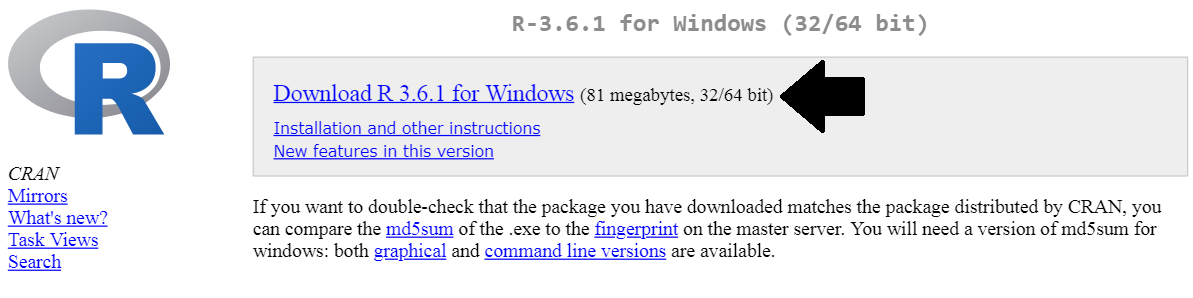
\includegraphics[width=1\linewidth]{images/OhdsiAnalyticsTools/downloadR} 

}

\caption{CRAN으로부터 R 다운로드}\label{fig:downloadR}
\end{figure}

\begin{enumerate}
\def\labelenumi{\arabic{enumi}.}
\setcounter{enumi}{1}
\tightlist
\item
  다운로드가 완료된 후 설치 프로그램을 실행하십시오. 다음 두 가지 예외를
  제외하고 모든 곳에서 기본 옵션을 사용하십시오. 첫째, 프로그램 파일에
  설치하지 않는 것이 좋다. 대신 R을 그림 \ref{fig:rDestination}과 같이 C
  드라이브의 하위 폴더로 만드십시오. 둘째, R과 Java 간의 아키텍처 차이로
  인한 문제를 방지하려면 그림 \ref{fig:no32Bits}과 같이 32-bit
  아키텍처를 비활성화 하십시오.
\end{enumerate}

\begin{figure}

{\centering 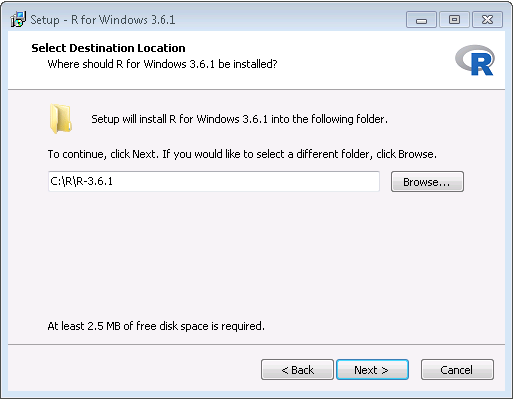
\includegraphics[width=0.8\linewidth]{images/OhdsiAnalyticsTools/rDestination} 

}

\caption{R의 대상 폴더를 설정하시오.}\label{fig:rDestination}
\end{figure}

\begin{figure}

{\centering 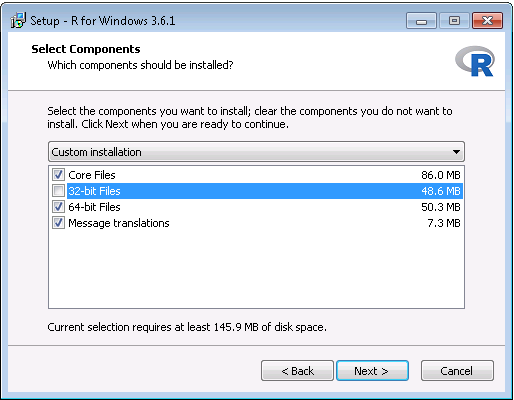
\includegraphics[width=0.8\linewidth]{images/OhdsiAnalyticsTools/no32Bits} 

}

\caption{32-bit 버전의 R을 사용하지 않도록 설정}\label{fig:no32Bits}
\end{figure}

완료되면 시작 메뉴에서 R을 선택할 수 있어야 한다.

\subsubsection*{Installing RTools}\label{installing-rtools}
\addcontentsline{toc}{subsubsection}{Installing RTools}

\begin{enumerate}
\def\labelenumi{\arabic{enumi}.}
\item
  \url{https://cran.r-project.org/},으로 이동하여 ``Windows용 R
  다운로드''를 클릭한 다음 ``Rtools''를 클릭하고 다운로드할 최신 버전의
  RTools를 선택하십시오.
\item
  다운로드가 완료된 후 설치 프로그램을 실행하십시오. 어디에서나 기본
  옵션을 선택하십시오.
\end{enumerate}

\subsubsection*{Installing RStudio}\label{installing-rstudio}
\addcontentsline{toc}{subsubsection}{Installing RStudio}

\begin{enumerate}
\def\labelenumi{\arabic{enumi}.}
\tightlist
\item
  \url{https://www.rstudio.com/}으로 이동하여, ``Download RStudio''을
  선택(또는 ``RStudio''에서 ``Download'' 버튼을 선택)하고, 무료 버전을
  선택한 후, 그림 \ref{fig:downloadRStudio}과 같이 Windows용 설치
  프로그램을 다운로드하십시오.
\end{enumerate}

\begin{figure}

{\centering 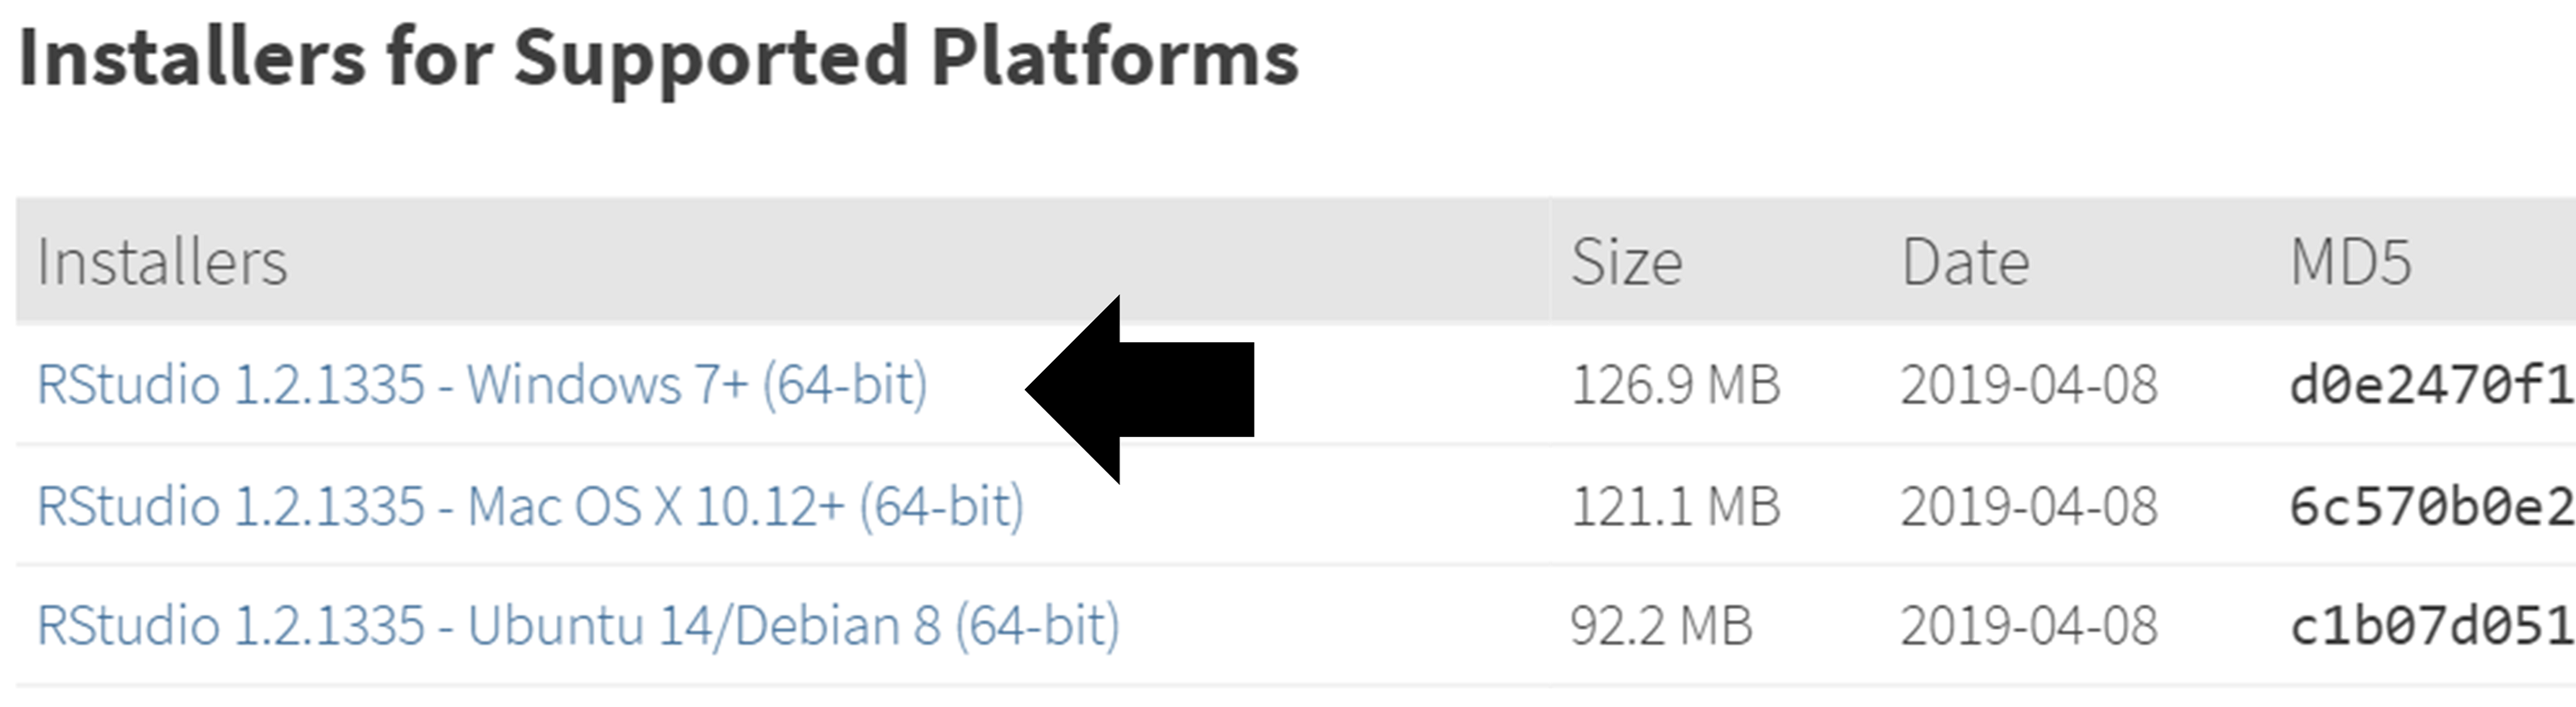
\includegraphics[width=1\linewidth]{images/OhdsiAnalyticsTools/downloadRStudio} 

}

\caption{RStudio 다운로드}\label{fig:downloadRStudio}
\end{figure}

\begin{enumerate}
\def\labelenumi{\arabic{enumi}.}
\setcounter{enumi}{1}
\tightlist
\item
  다운로드한 후, 설치 관리자를 시작하고, 모든 곳에서 기본 옵션을
  선택하십시오.
\end{enumerate}

\subsubsection*{Installing Java}\label{installing-java}
\addcontentsline{toc}{subsubsection}{Installing Java}

\begin{enumerate}
\def\labelenumi{\arabic{enumi}.}
\tightlist
\item
  \url{https://java.com/en/download/manual.jsp}으로 이동하여, 그림
  \ref{fig:downloadJava}와 같이 Windows 64-bit installer를 선택하십시오.
  32-bit 버전의 R도 설치한 경우 \emph{반드시} 다른 32-bit 버전의 Java도
  설치해야 한다.
\end{enumerate}

\begin{figure}

{\centering 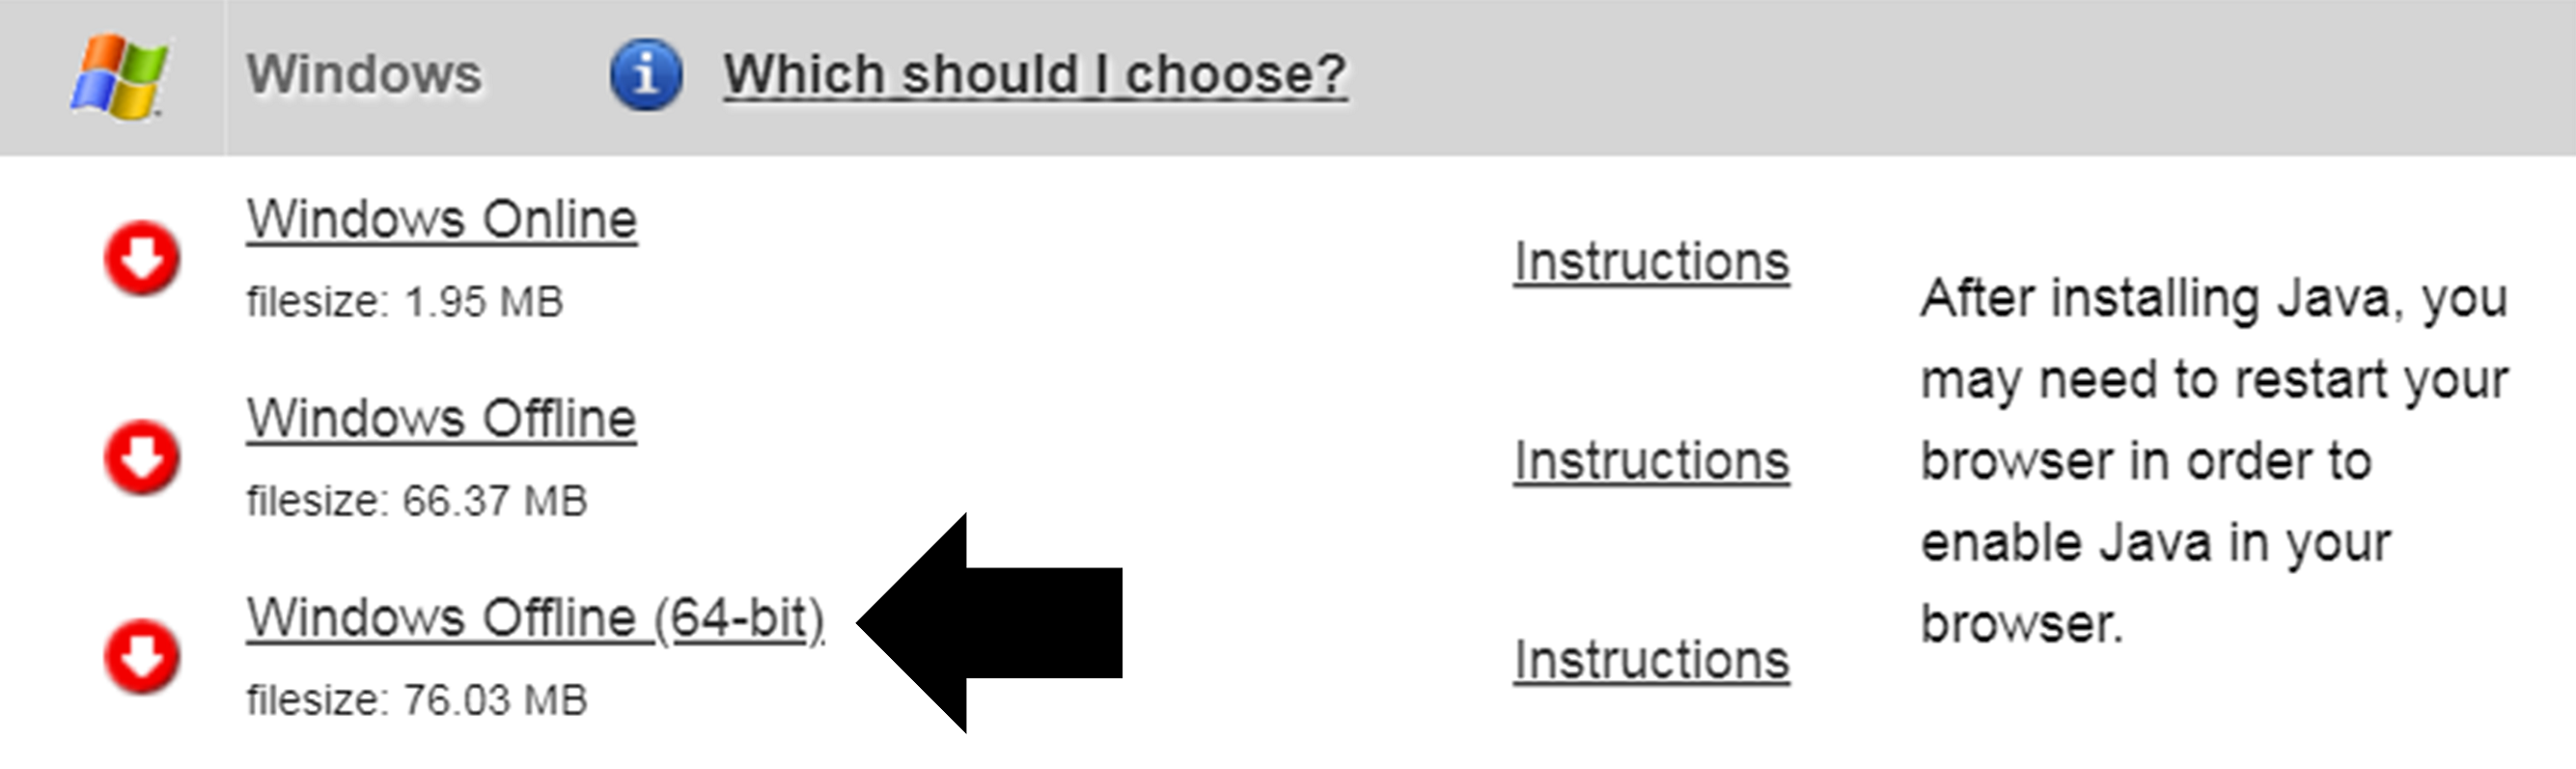
\includegraphics[width=1\linewidth]{images/OhdsiAnalyticsTools/downloadJava} 

}

\caption{Java 다운로드}\label{fig:downloadJava}
\end{figure}

\begin{enumerate}
\def\labelenumi{\arabic{enumi}.}
\setcounter{enumi}{1}
\tightlist
\item
  다운로드한 후 설치 프로그램을 실행하십시오.
\end{enumerate}

\subsubsection*{Verifying the
Installation}\label{verifying-the-installation}
\addcontentsline{toc}{subsubsection}{Verifying the Installation}

이제 시작할 준비를 해야 하지만, 그 전에 확실히 해야 한다. RStudio를
시작하고 및 아래의 내용을 입력하자.

\begin{Shaded}
\begin{Highlighting}[]
\KeywordTok{install.packages}\NormalTok{(}\StringTok{"SqlRender"}\NormalTok{)}
\KeywordTok{library}\NormalTok{(SqlRender)}
\KeywordTok{translate}\NormalTok{(}\StringTok{"SELECT TOP 10 * FROM person;"}\NormalTok{, }\StringTok{"postgresql"}\NormalTok{)}
\end{Highlighting}
\end{Shaded}

\begin{verbatim}
## [1] "SELECT  * FROM person LIMIT 10;"
\end{verbatim}

이 기능은 Java를 사용하기 때문에, 만약 모든 것이 잘 된다면, R과 Java가
모두 올바르게 설치되었다는 것을 알 수 있다!

또 다른 테스트는 소스 패키지를 제대로 구축할 수 있는지 확인하는 것이다.
다음 R 코드를 실행하여 OHDSI GitHub 저장소에서 \texttt{CohortMethod}
패키지를 설치하십시오:

\begin{Shaded}
\begin{Highlighting}[]
\KeywordTok{install.packages}\NormalTok{(}\StringTok{"drat"}\NormalTok{)}
\NormalTok{drat}\OperatorTok{::}\KeywordTok{addRepo}\NormalTok{(}\StringTok{"OHDSI"}\NormalTok{)}
\KeywordTok{install.packages}\NormalTok{(}\StringTok{"CohortMethod"}\NormalTok{)}
\end{Highlighting}
\end{Shaded}

\section{Deployment Strategies}\label{deployment-strategies}

ATLAS 및 Method Library를 포함한 전체 OHDSI 도구 스택을 조직에 배치하는
것은 어려운 작업이다. 의존성 높은 구성 요소들을 많이 고려해야 하고,
설정해야 할 환경이 많다. 이 때문에 두 이니셔티브(Broadsea와 AWS(Amazon
Web Services))는 일부 가상화 형태를 이용해 전체 스택을 하나의 패키지로
설치할 수 있는 통합 배치 전략을 개발했다. \index{tools deployment}

\subsection{Broadsea}\label{broadsea}

Broadsea\footnote{\url{https://github.com/OHDSI/Broadsea}}은 Docker
컨테이너 기술을 사용한다.\footnote{\url{https://www.docker.com/}} OHDSI
도구는 의존성과 함께 Docker Image라는 단일 휴대용 이진 파일로
패키징된다. 그러면 이 이미지는 Docker 엔진 서비스에서 실행되고, 모든
소프트웨어가 설치되어 실행 준비가 된 가상 시스템(virtual machine)을
생성할 수 있다. Docker 엔진은 마이크로소프트 윈도우, 맥OS, 리눅스를
포함한 대부분의 운영 체제에 사용할 수 있다. Broadsea Docker 이미지에는
Methods Library와 ATLAS를 포함한 주요 OHDSI 도구가 포함되어 있다.
\index{tools deployment!Broadsea}

\subsection{Amazon AWS}\label{amazon-aws}

Amazon은 버튼 클릭 한 번으로 AWS 클라우드 컴퓨팅 환경에서 인스턴스화할
수 있는 두 가지 환경, 즉 OHDSI-in-a-Box\footnote{\url{https://github.com/OHDSI/OHDSI-in-a-Box}}와
OHDSIonAWS.\footnote{\url{https://github.com/OHDSI/OHDSIonAWS}}을
준비했다. \index{tools deployment!Amazon AWS}

OHDSI-in-a-Box is specifically created as a learning environment, and is
used in most of the tutorials provided by the OHDSI community. It
includes many OHDSI tools, sample data sets, RStudio and other
supporting software in a single, low cost Windows virtual machine. A
PostgreSQL database is used to store the CDM and also to store the
intermediary results from ATLAS. The OMOP CDM data mapping and ETL tools
are also included in OHDSI-in-a-Box. The architecture for OHDSI-in-a-Box
is depicted in Figure \ref{fig:ohdsiinaboxDiagram}.

OHDSI-in-a-Box는 특별히 학습 환경으로 만들어졌으며, OHDSI 커뮤니티에서
제공하는 대부분의 튜토리얼에 사용된다. 그것은 많은 OHDSI 도구, 샘플
데이터 세트, RStudio 및 기타 지원 소프트웨어를 저렴한 단일 윈도우즈 가상
머신에 포함한다. PostgreSQL 데이터베이스는 CDM을 저장하고 ATLAS의 중간
결과를 저장하는 데 사용된다. OMOP CDM 데이터 매핑과 ETL 툴도
OHDSI-in-a-Box에 포함되어 있다. OHDSI-in-a-Box 아키텍처는 그림
\ref{fig:ohdsiinaboxDiagram}에 나타나 있다.

\begin{figure}

{\centering 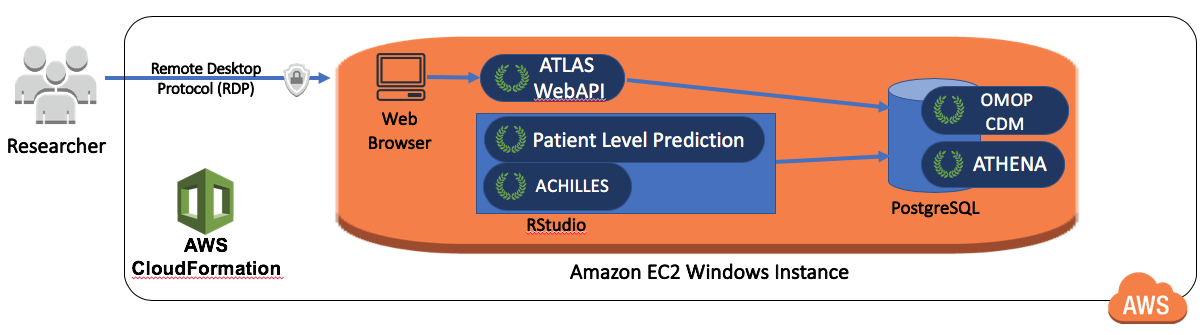
\includegraphics[width=1\linewidth]{images/OhdsiAnalyticsTools/OHDSI-in-a-BoxDiagram} 

}

\caption{OHDSI-in-a-Box용 Amazon Web Services 아키텍처}\label{fig:ohdsiinaboxDiagram}
\end{figure}

OHDSIonAWS는 조직이 그들의 데이터 분석을 수행하는 데 사용할 수 있는
엔터프라이즈급, 다중 사용자, 확장 가능하고 내결함성 OHDSI 환경을 위한
참조 아키텍처다. 여기에는 몇 가지 샘플 데이터 세트가 포함되어 있으며
조직의 실제 의료 데이터를 자동으로 적재할 수도 있다. 데이터는 OHDSI
도구에 의해 지원되는 Amazon Redshift 데이터베이스 플랫폼에 배치된다.
ATLAS의 중간 결과는 PostgreSQL 데이터베이스에 저장된다. 프런트 엔드에서
사용자는 웹 인터페이스(leveraging RStudio Server)를 통해 ATLAS와
RStudio에 접근할 수 있다. RStudio에는 OHDSI Methods Library가 이미
설치되어 있으며, 데이터베이스에 연결하는 데 사용할 수 있다. OHDSIonAWS를
배포하는 자동화는 오픈 소스로, 조직의 관리 툴과 모범 사례를 포함하도록
사용자 정의할 수 있다. OHDSIonAWS에 대한 아키텍처는 그림
\ref{fig:ohdsionawsDiagram}에 설명되어 있다.

\begin{figure}

{\centering 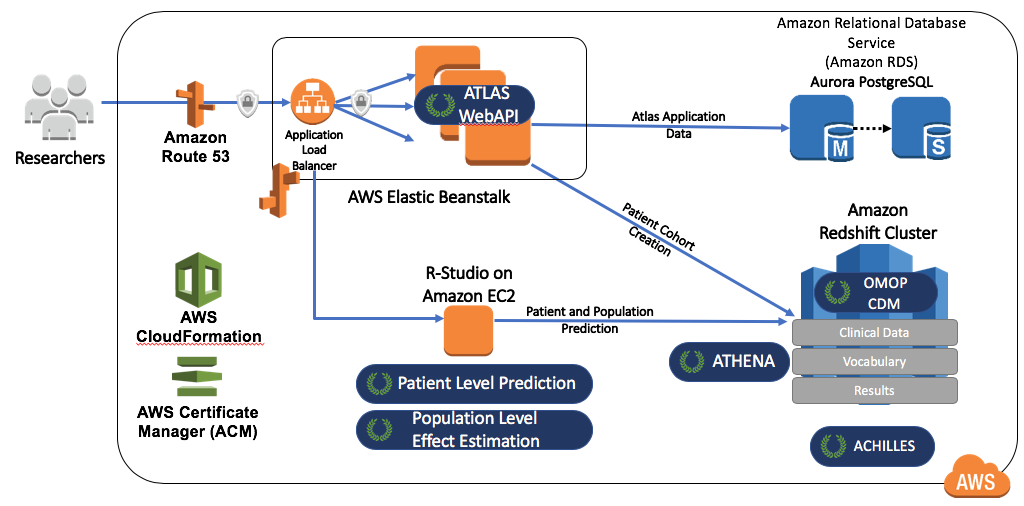
\includegraphics[width=1\linewidth]{images/OhdsiAnalyticsTools/OHDSIonAWSDiagram} 

}

\caption{OHDSIonAWS를 위한 Amazon Web Services 아카이브}\label{fig:ohdsionawsDiagram}
\end{figure}

\section{Summary}\label{summary-2}

\BeginKnitrBlock{rmdsummary}
\begin{itemize}
\tightlist
\item
  다음을 통해 CDM의 데이터에 대한 분석을 수행할 수 있다.

  \begin{itemize}
  \tightlist
  \item
    사용자 지정 코드 작성
  \item
    OHDSI Method Library에서 R 패키지를 사용하는 코드 작성
  \item
    대화형 분석 플랫폼 ATLAS 사용
  \end{itemize}
\item
  OHDSI 툴은 다양한 분석 전략을 사용한다.

  \begin{itemize}
  \tightlist
  \item
    단일 연구
  \item
    실시간 쿼리
  \item
    대규모 분석
  \end{itemize}
\item
  대부분의 OHDSI 분석 툴이 다음에 내장되어 있다.

  \begin{itemize}
  \tightlist
  \item
    대화형 분석 플랫폼 ATLAS
  \item
    OHDSI Methods Library R 패키지
  \end{itemize}
\item
  OHDSI 툴의 구축을 촉진하는 몇 가지 전략이 존재한다.
\end{itemize}
\EndKnitrBlock{rmdsummary}

\chapter{SQL and R}\label{SqlAndR}

\emph{Chapter leads: Martijn Schuemie \& Peter Rijnbeek}

공통 데이터 모델(Common Data Model, CDM)은 모든 데이터가 필드가 있는
테이블의 레코드로 표시되는 관계형 데이터베이스 모델입니다. 이는
일반적으로 PostgreSQL, Oracle, Microsoft SQL Server와 같은 소프트웨어
플랫폼을 사용하여 데이터가 관계형 데이터 베이스에 저장된다는 것을
의미합니다. ATLAS와 Methods Library 같은 다양한 OHDSI 도구는
백그라운드에서 데이터베이스에 질의하여 작동하지만 적절한 접근 권한이
있으면 직접 데이터베이스에 질의할 수도 있습니다. 데이터베이스에 직접
질의하는 주된 이유는 현재 기존 도구가 지원하지 않는 분석을 수행하기 위한
것입니다. 그러나 OHDSI 도구는 보통 사용자가 데이터를 적절하게 분석을 할
수 있는 지침을 안내하도록 설계되어 있기 때문에 직접 데이터베이스에
질의하는 것은 실수를 범할 위험이 더 커집니다. 직접 질의하는 것은 그런
지침을 제공하지 않습니다. 관계형 데이터베이스에 질의하기 위한 표준
언어는 Structured Query Language (SQL)이며, 이는 데이터에 대한 변경 뿐만
아니라 데이터베이스에 대한 질의를 위해 사용할 수 있다. SQL의 기본
명령어는 실제로 표준이고 소프트웨어 플랫폼 전반에 걸쳐 동일한 의미를
가지지만, 각 플랫폼마다 미묘한 변경이 있는 고유한 문법을 가지고
있습니다. 예를 들면, SQL Server에서 PERSON 테이블에서 상위 10개의 행을
검색하려면 다음을 입력합니다: \index{SQL}
\index{structured query language|see {SQL}}

\begin{Shaded}
\begin{Highlighting}[]
\KeywordTok{SELECT}\NormalTok{ TOP }\DecValTok{10}\NormalTok{ * }\KeywordTok{FROM}\NormalTok{ person;}
\end{Highlighting}
\end{Shaded}

PostgreSQL의 동일한 질의는 다음과 같습니다:

\begin{Shaded}
\begin{Highlighting}[]
\KeywordTok{SELECT}\NormalTok{ * }\KeywordTok{FROM}\NormalTok{ person }\KeywordTok{LIMIT} \DecValTok{10}\NormalTok{;}
\end{Highlighting}
\end{Shaded}

OHDSI에서는 플랫폼이 사용하는 고유한 문법에 구애받지 않고 모든 OHDSI
데이터베이스에서 동일한 SQL 언어를 사용하고자 합니다. 이러한 이유로
OHDSI는 이 장의 뒤에서 논의하게 될, 하나의 표준 문법을 다른 여러 개의
문법으로 번역해줄 수 있는 패키지인
\href{https://ohdsi.github.io/SqlRender/}{SqlRender} 를 개발했습니다. 이
표준 언어 - \textbf{OHDSI SQL} - 는 주로 SQL Server SQL 언어의 하위
집합입니다. 이 장에서 제공되는 SQL 문 예는 모두 OHDSI SQL을 사용합니다.
\index{SqlRender} \index{agnostic SQL|see {SqlRender}}
\index{Standard SQL Dialect|see {SqlRender}}
\index{OHDSI SQL|see {SqlRender}}

각 데이터베이스 플랫폼에는 SQL을 사용하여 데이터베이스를 질의하기 위한
자체 소프트웨어 도구가 제공됩니다. OHDSI는 여러 데이터베이스 플랫폼에
연결할 수 있는 하나의 R 패키지인
\href{https://ohdsi.github.io/DatabaseConnector/}{DatabaseConnector} 를
개발했습니다. DatabaseConnector도 이 장의 뒤에서 논의할 것입니다.
\index{DatabaseConnector}

따라서 OHDSI 도구를 사용하지 않고 CDM에 맞게 질의할 수 있지만
DatabaseConnector 및 SqlRender 패키지를 사용하는 것을 권장합니다. 이를
통해 한 사이트에서 개발된 질의를 수정하지 않고 다른 사이트에서 사용할 수
있습니다. R 자체는 통계 분석 및 대화식 그래프 생성과 같이
데이터베이스에서 추출된 데이터를 추가로 분석하는 기능도 직접 제공합니다.
\index{R}

이 장에서는 독자가 SQL에 대한 기본 지식을 가지고 있다고 가정합니다. 먼저
SqlRender 및 DatabaseConnector 사용 방법을 검토합니다. 독자가 이
패키지를 사용할 의도가 없는 경우 이 절은 건너 뛸 수 있습니다.
\ref{QueryTheCdm} 절에서는 SQL (OHDSI SQL)을 사용하여 CDM에 질의하는
방법에 대해 설명합니다. 그 다음 절에서는 CDM에 질의할 때 OHDSI 표준
용어를 사용하는 방법을 강조합니다. 공개적으로 이용 가능한 CDM에 대해
일반적으로 사용되는 질의 모음인 QueryLibrary를 강조합니다. 발생률을
추정하는 예제 연구로 이 장을 마무리하고 SqlRender 및 DatabaseConnector를
사용하여 이 연구를 구현합니다. \index{Query Library}
\index{SQL Query Libary|see {Query Library}}

\hypertarget{SqlRender}{\section{SqlRender}\label{SqlRender}}

\href{https://ohdsi.github.io/SqlRender/}{SqlRender} 패키지는
Comprehensive R Archive Network (CRAN)에서 이용할 수 있으므로 다음을
사용하여 설치할 수 있습니다:

\begin{Shaded}
\begin{Highlighting}[]
\KeywordTok{install.packages}\NormalTok{(}\StringTok{"SqlRender"}\NormalTok{)}
\end{Highlighting}
\end{Shaded}

SqlRender는 전통적인 데이터베이스 시스템(PostgreSQL, Microsoft SQL
Server, SQLite, and Oracle), 병렬 데이터 웨어하우스(Microsoft APS, IBM
Netezza, and Amazon RedShift), 빅데이터 플랫폼(Hadoop through Impala,
and Google BigQuery)을 포함한 다수의 기술 플랫폼을 지원합니다.

\subsection{SQL Parameterization}\label{sql-parameterization}

패키지의 기능 중 하나는 SQL의 매개 변수화를 지원하는 것입니다. 일부 매개
변수에 기반하여 SQL의 작은 변형들을 생성할 필요가 종종 있습니다.
SqlRender는 매개 변수화를 허용하기 위해 SQL 코드 내에서 간단한 마크업
구문을 제공합니다. 매개 변수를 기반으로 SQL을 렌더링하는 것은
\texttt{render()} 함수를 사용하여 수행됩니다.
\index{SqlRender!parameterization}

\subsubsection*{Substituting Parameter
Values}\label{substituting-parameter-values}
\addcontentsline{toc}{subsubsection}{Substituting Parameter Values}

\texttt{@} 문자는 렌더링 시 실제 매개 변수 값과 교환해야하는 매개 변수
이름을 나타내는데 사용할 수 있습니다. 다음 예에서 \texttt{a}라고 불리는
변수가 SQL에서 언급되어 있습니다. 렌더 함수를 호출할 때 이 매개 변수의
값이 정의됩니다:

\begin{Shaded}
\begin{Highlighting}[]
\NormalTok{sql <-}\StringTok{ "SELECT * FROM concept WHERE concept_id = @a;"}
\KeywordTok{render}\NormalTok{(sql, }\DataTypeTok{a =} \DecValTok{123}\NormalTok{)}
\end{Highlighting}
\end{Shaded}

\begin{verbatim}
## [1] "SELECT * FROM concept WHERE concept_id = 123;"
\end{verbatim}

대부분의 데이터베이스 관리 시스템에서 제공하는 매개 변수화와 달리 테이블
또는 필드 이름을 값으로 매개 변수화 하는 것이 쉽다는 것에 주목하십시오:

\begin{Shaded}
\begin{Highlighting}[]
\NormalTok{sql <-}\StringTok{ "SELECT * FROM @x WHERE person_id = @a;"}
\KeywordTok{render}\NormalTok{(sql, }\DataTypeTok{x =} \StringTok{"observation"}\NormalTok{, }\DataTypeTok{a =} \DecValTok{123}\NormalTok{)}
\end{Highlighting}
\end{Shaded}

\begin{verbatim}
## [1] "SELECT * FROM observation WHERE person_id = 123;"
\end{verbatim}

매개 변수 값은 숫자, 문자열, 부울 및 쉼표를 기준으로 항목을 나눈
리스트로 변환된 벡터일 수 있습니다:

\begin{Shaded}
\begin{Highlighting}[]
\NormalTok{sql <-}\StringTok{ "SELECT * FROM concept WHERE concept_id IN (@a);"}
\KeywordTok{render}\NormalTok{(sql, }\DataTypeTok{a =} \KeywordTok{c}\NormalTok{(}\DecValTok{123}\NormalTok{, }\DecValTok{234}\NormalTok{, }\DecValTok{345}\NormalTok{))}
\end{Highlighting}
\end{Shaded}

\begin{verbatim}
## [1] "SELECT * FROM concept WHERE concept_id IN (123,234,345);"
\end{verbatim}

\subsubsection*{If-Then-Else}\label{if-then-else}
\addcontentsline{toc}{subsubsection}{If-Then-Else}

때로는 하나 이상의 매개 변수 값에 따라 코드 블록을 켜거나 끌 필요가
있습니다. 이 작업은
\texttt{\{Condition\}\ ?\ \{if\ true\}\ :\ \{if\ false\}} 구문을
사용합니다. \emph{조건}이 참 또는 1로 평가되면, \emph{if true} 블록을
사용되고 그렇지 않으면, \emph{if false} 블록이 표시됩니다(있는 경우).

\begin{Shaded}
\begin{Highlighting}[]
\NormalTok{sql <-}\StringTok{ "SELECT * FROM cohort \{@x\} ? \{WHERE subject_id = 1\}"}
\KeywordTok{render}\NormalTok{(sql, }\DataTypeTok{x =} \OtherTok{FALSE}\NormalTok{)}
\end{Highlighting}
\end{Shaded}

\begin{verbatim}
## [1] "SELECT * FROM cohort "
\end{verbatim}

\begin{Shaded}
\begin{Highlighting}[]
\KeywordTok{render}\NormalTok{(sql, }\DataTypeTok{x =} \OtherTok{TRUE}\NormalTok{)}
\end{Highlighting}
\end{Shaded}

\begin{verbatim}
## [1] "SELECT * FROM cohort WHERE subject_id = 1"
\end{verbatim}

간단한 비교도 지원됩니다:

\begin{Shaded}
\begin{Highlighting}[]
\NormalTok{sql <-}\StringTok{ "SELECT * FROM cohort \{@x == 1\} ? \{WHERE subject_id = 1\};"}
\KeywordTok{render}\NormalTok{(sql, }\DataTypeTok{x =} \DecValTok{1}\NormalTok{)}
\end{Highlighting}
\end{Shaded}

\begin{verbatim}
## [1] "SELECT * FROM cohort WHERE subject_id = 1;"
\end{verbatim}

\begin{Shaded}
\begin{Highlighting}[]
\KeywordTok{render}\NormalTok{(sql, }\DataTypeTok{x =} \DecValTok{2}\NormalTok{)}
\end{Highlighting}
\end{Shaded}

\begin{verbatim}
## [1] "SELECT * FROM cohort ;"
\end{verbatim}

IN 연산자도 지원됩니다:

\begin{Shaded}
\begin{Highlighting}[]
\NormalTok{sql <-}\StringTok{ "SELECT * FROM cohort \{@x IN (1,2,3)\} ? \{WHERE subject_id = 1\};"}
\KeywordTok{render}\NormalTok{(sql, }\DataTypeTok{x =} \DecValTok{2}\NormalTok{)}
\end{Highlighting}
\end{Shaded}

\begin{verbatim}
## [1] "SELECT * FROM cohort WHERE subject_id = 1;"
\end{verbatim}

\subsection{Translation to Other SQL
Dialects}\label{translation-to-other-sql-dialects}

\href{https://ohdsi.github.io/SqlRender/}{SqlRender} 패키지의 또 다른
기능은 OHDSI SQL에서 다른 SQL 언어로 변환하는 것입니다. 예를 들면 다음과
같습니다:

\begin{Shaded}
\begin{Highlighting}[]
\NormalTok{sql <-}\StringTok{ "SELECT TOP 10 * FROM person;"}
\KeywordTok{translate}\NormalTok{(sql, }\DataTypeTok{targetDialect =} \StringTok{"postgresql"}\NormalTok{)}
\end{Highlighting}
\end{Shaded}

\begin{verbatim}
## [1] "SELECT  * FROM person LIMIT 10;"
\end{verbatim}

\texttt{targetDialect} 매개 변수는 다음과 같은 값을 가질 수 있습니다:
``oracle'', ``postgresql'', ``pdw''``,''redshift``'', ``impala'',
``netezza'', ``bigquery'', ``sqlite'', and ``sql server''.
\index{SqlRender!translation}

\BeginKnitrBlock{rmdimportant}
패키지에는 제한된 변환 규칙 세트만 구현되었기 때문에 SQL의 함수 및
구성을 적절하게 번역되는 것에는 한계가 있을 뿐 아니라 일부 SQL의 특징은
모든 언어에서 동일하지 않습니다. OHDSI SQL이 독자적인 새로운 문법으로
개발된 주된 이유입니다. 하지만 이미 있는 것을 다시 만드느라 쓸데없이
시간을 낭비하지 않기 위해 SQL Server 구문을 유지했습니다.
\EndKnitrBlock{rmdimportant}

최선의 노력에도 불구하고, 지원되는 모든 플랫폼에서 오류없이 실행될 OHDSI
SQL을 작성할 때 고려해야 할 사항이 몇 가지 있습니다. 다음은 이러한 고려
사항에 대해 자세히 설명합니다.

\subsubsection*{Functions and Structures Supported By
Translate}\label{functions-and-structures-supported-by-translate}
\addcontentsline{toc}{subsubsection}{Functions and Structures Supported
By Translate}

다음과 같은 SQL Server 함수는 테스트되었으며 다양한 언어로 올바르게 번환
되는 것으로 밝혀졌습니다: \index{SqlRender!supported functions}

\begin{longtable}[]{@{}lll@{}}
\caption{\label{tab:sqlFunctions} Functions supported by
translate.}\tabularnewline
\toprule
Function & Function & Function\tabularnewline
\midrule
\endfirsthead
\toprule
Function & Function & Function\tabularnewline
\midrule
\endhead
ABS & EXP & RAND\tabularnewline
ACOS & FLOOR & RANK\tabularnewline
ASIN & GETDATE & RIGHT\tabularnewline
ATAN & HASHBYTES* & ROUND\tabularnewline
AVG & ISNULL & ROW\_NUMBER\tabularnewline
CAST & ISNUMERIC & RTRIM\tabularnewline
CEILING & LEFT & SIN\tabularnewline
CHARINDEX & LEN & SQRT\tabularnewline
CONCAT & LOG & SQUARE\tabularnewline
COS & LOG10 & STDEV\tabularnewline
COUNT & LOWER & SUM\tabularnewline
COUNT\_BIG & LTRIM & TAN\tabularnewline
DATEADD & MAX & UPPER\tabularnewline
DATEDIFF & MIN & VAR\tabularnewline
DATEFROMPARTS & MONTH & YEAR\tabularnewline
DATETIMEFROMPARTS & NEWID &\tabularnewline
DAY & PI &\tabularnewline
EOMONTH & POWER &\tabularnewline
\bottomrule
\end{longtable}

* Oracle은 특별 권한이 필요합니다. SQLite에는 해당되는 것이 없습니다.

마찬가지로 많은 SQL 구문 구조가 지원됩니다. 다음은 우리가 잘 번역할 수
있는 표현식의 전체 목록입니다:

\begin{Shaded}
\begin{Highlighting}[]
\CommentTok{-- Simple selects:}
\KeywordTok{SELECT}\NormalTok{ * }\KeywordTok{FROM} \KeywordTok{table}\NormalTok{;}

\CommentTok{-- Selects with joins:}
\KeywordTok{SELECT}\NormalTok{ * }\KeywordTok{FROM}\NormalTok{ table_1 }\KeywordTok{INNER} \KeywordTok{JOIN}\NormalTok{ table_2 }\KeywordTok{ON}\NormalTok{ a = b;}

\CommentTok{-- Nested queries:}
\KeywordTok{SELECT}\NormalTok{ * }\KeywordTok{FROM}\NormalTok{ (}\KeywordTok{SELECT}\NormalTok{ * }\KeywordTok{FROM}\NormalTok{ table_1) tmp }\KeywordTok{WHERE}\NormalTok{ a = b;}

\CommentTok{-- Limiting to top rows:}
\KeywordTok{SELECT}\NormalTok{ TOP }\DecValTok{10}\NormalTok{ * }\KeywordTok{FROM} \KeywordTok{table}\NormalTok{;}

\CommentTok{-- Selecting into a new table:}
\KeywordTok{SELECT}\NormalTok{ * }\KeywordTok{INTO}\NormalTok{ new_table }\KeywordTok{FROM} \KeywordTok{table}\NormalTok{;}

\CommentTok{-- Creating tables:}
\KeywordTok{CREATE} \KeywordTok{TABLE} \KeywordTok{table}\NormalTok{ (field }\DataTypeTok{INT}\NormalTok{);}

\CommentTok{-- Inserting verbatim values:}
\KeywordTok{INSERT} \KeywordTok{INTO}\NormalTok{ other_table (field_1) }\KeywordTok{VALUES}\NormalTok{ (}\DecValTok{1}\NormalTok{);}

\CommentTok{-- Inserting from SELECT:}
\KeywordTok{INSERT} \KeywordTok{INTO}\NormalTok{ other_table (field_1) }\KeywordTok{SELECT} \FunctionTok{value} \KeywordTok{FROM} \KeywordTok{table}\NormalTok{;}
  
\CommentTok{-- Simple drop commands:}
\KeywordTok{DROP} \KeywordTok{TABLE} \KeywordTok{table}\NormalTok{;}

\CommentTok{-- Drop table if it exists:}
\KeywordTok{IF}\NormalTok{ OBJECT_ID(}\StringTok{'ACHILLES_analysis'}\NormalTok{, }\StringTok{'U'}\NormalTok{) }\KeywordTok{IS} \KeywordTok{NOT} \KeywordTok{NULL}
  \KeywordTok{DROP} \KeywordTok{TABLE}\NormalTok{ ACHILLES_analysis;}
  
\CommentTok{-- Drop temp table if it exists:}
\KeywordTok{IF}\NormalTok{ OBJECT_ID(}\StringTok{'tempdb..#cohorts'}\NormalTok{, }\StringTok{'U'}\NormalTok{) }\KeywordTok{IS} \KeywordTok{NOT} \KeywordTok{NULL}
  \KeywordTok{DROP} \KeywordTok{TABLE}\NormalTok{ #cohorts;  }

\CommentTok{-- Common table expressions:}
\KeywordTok{WITH}\NormalTok{ cte }\KeywordTok{AS}\NormalTok{ (}\KeywordTok{SELECT}\NormalTok{ * }\KeywordTok{FROM} \KeywordTok{table}\NormalTok{) }\KeywordTok{SELECT}\NormalTok{ * }\KeywordTok{FROM}\NormalTok{ cte;}

\CommentTok{-- OVER clauses:}
\KeywordTok{SELECT} \FunctionTok{ROW_NUMBER}\NormalTok{() }\KeywordTok{OVER}\NormalTok{ (}\KeywordTok{PARTITION} \KeywordTok{BY}\NormalTok{ a }\KeywordTok{ORDER} \KeywordTok{BY}\NormalTok{ b)}
  \KeywordTok{AS} \OtherTok{"Row Number"} \KeywordTok{FROM} \KeywordTok{table}\NormalTok{;}
  
\CommentTok{-- CASE WHEN clauses:}
\KeywordTok{SELECT} \KeywordTok{CASE} \KeywordTok{WHEN}\NormalTok{ a=}\DecValTok{1} \KeywordTok{THEN}\NormalTok{ a }\KeywordTok{ELSE} \DecValTok{0} \KeywordTok{END} \KeywordTok{AS} \FunctionTok{value} \KeywordTok{FROM} \KeywordTok{table}\NormalTok{;}

\CommentTok{-- UNIONs:}
\KeywordTok{SELECT}\NormalTok{ * }\KeywordTok{FROM}\NormalTok{ a }\KeywordTok{UNION} \KeywordTok{SELECT}\NormalTok{ * }\KeywordTok{FROM}\NormalTok{ b;}

\CommentTok{-- INTERSECTIONs:}
\KeywordTok{SELECT}\NormalTok{ * }\KeywordTok{FROM}\NormalTok{ a }\KeywordTok{INTERSECT} \KeywordTok{SELECT}\NormalTok{ * }\KeywordTok{FROM}\NormalTok{ b;}

\CommentTok{-- EXCEPT:}
\KeywordTok{SELECT}\NormalTok{ * }\KeywordTok{FROM}\NormalTok{ a }\KeywordTok{EXCEPT} \KeywordTok{SELECT}\NormalTok{ * }\KeywordTok{FROM}\NormalTok{ b;}
\end{Highlighting}
\end{Shaded}

\subsubsection*{String Concatenation}\label{string-concatenation}
\addcontentsline{toc}{subsubsection}{String Concatenation}

문자열 연결은 SQL Server가 다른 언어보다 덜 구체적인 영역입니다. SQL
Server에서는
\texttt{SELECT\ first\_name\ +\ \textquotesingle{}\ \textquotesingle{}\ +\ last\_name\ AS\ full\_name\ FROM\ table}와
같이 작성하지만 Postgres와 Oracle에서는
\texttt{SELECT\ first\_name\ \textbar{}\textbar{}\ \textquotesingle{}\ \textquotesingle{}\ \textbar{}\textbar{}\ last\_name\ AS\ full\_name\ FROM\ table}
라고 작성합니다. SqlRender는 연결되는 값이 문자열인지 추측하려고 합니다.
위의 예에서 명시적인 문자열(작은 따옴표로 묶인 공백)이 있음으로 번역은
정확할 것입니다. 그러나
\texttt{SELECT\ first\_name\ +\ last\_name\ AS\ full\_name\ FROM\ table}와
같이 작성한다면 SqlRender는 두 필드가 문자열이라는 단서가 없으며, 잘못된
더하기 기호를 남겼습니다. 값이 문자열이라는 또 다른 단서는 ``VARCHAR''에
대한 명시적 형변환이므로
\texttt{SELECT\ last\_name\ +\ CAST(age\ AS\ VARCHAR(3))\ AS\ full\_name\ FROM\ table}
도 올바르게 변환됩니다. 모호성을 피하려면 \texttt{CONCAT()} 함수를
사용하여 두개 이상의 문자열을 연결하는 것이 가장 좋습니다.

\subsubsection*{Table Aliases and the AS
Keyword}\label{table-aliases-and-the-as-keyword}
\addcontentsline{toc}{subsubsection}{Table Aliases and the AS Keyword}

많은 SQL 언어는 테이블 별칭을 정의할 때 \texttt{AS} 키워드를 사용할 수
있지만 키워드 없이도 잘 동작 합니다. 예를 들어, 이 두 SQL 문은 SQL
Server, PostgreSQL, RedShift 등에 적합합니다:

\begin{Shaded}
\begin{Highlighting}[]
\CommentTok{-- Using AS keyword}
\KeywordTok{SELECT}\NormalTok{ * }
\KeywordTok{FROM}\NormalTok{ my_table }\KeywordTok{AS}\NormalTok{ table_}\DecValTok{1}
\KeywordTok{INNER} \KeywordTok{JOIN}\NormalTok{ (}
  \KeywordTok{SELECT}\NormalTok{ * }\KeywordTok{FROM}\NormalTok{ other_table}
\NormalTok{) }\KeywordTok{AS}\NormalTok{ table_}\DecValTok{2}
\KeywordTok{ON}\NormalTok{ table_1.person_id = table_2.person_id;}

\CommentTok{-- Not using AS keyword}
\KeywordTok{SELECT}\NormalTok{ * }
\KeywordTok{FROM}\NormalTok{ my_table table_}\DecValTok{1}
\KeywordTok{INNER} \KeywordTok{JOIN}\NormalTok{ (}
  \KeywordTok{SELECT}\NormalTok{ * }\KeywordTok{FROM}\NormalTok{ other_table}
\NormalTok{) table_}\DecValTok{2}
\KeywordTok{ON}\NormalTok{ table_1.person_id = table_2.person_id;}
\end{Highlighting}
\end{Shaded}

그러나 Oracle에서는 \texttt{AS} 키워드를 사용하면 오류가 발생합니다.
위의 예제 중 첫번째 질의는 실패합니다. 따라서 테이블 별칭을 지정할 때
\texttt{AS} 키워드를 사용하지 않는 것이 좋습니다. (참고: Oracle에서
\texttt{AS}를 사용할 수 없는 테이블 별칭과 이 \texttt{AS} 를 사용해야
하는 필드 별칭을 쉽게 구별할 수 없기 때문에 SqlRender가 이 것을
처리하도록 만들 수 없습니다.)

\subsubsection*{Temp Tables}\label{temp-tables}
\addcontentsline{toc}{subsubsection}{Temp Tables}

임시 테이블은 중간 결과를 저장하는 데 매우 유용할 수 있으며 올바르게
사용하면 질의 성능을 크게 향상시킬 수 있습니다. 대부분의 데이터베이스
플랫폼에서 임시 테이블의 매우 좋은 속성을 가지고 있습니다: 현재
사용자에게만 보이며 세션이 끝나면 자동으로 삭제되고 사용자에게 쓰기
권한이 없어도 생성할 수 있습니다. 불행히도, Oracle에서 임시테이블은
기본적으로 영구적인 테이블이며, 데이터의 내부는 현재 사용자에게만
보인다는 차이점만 있습니다. 이것이 Oracle에서 SqlRender가 다음을 통해
임시 테이블을 에뮬레이션 하려고 시도하는 이유입니다

\begin{enumerate}
\def\labelenumi{\arabic{enumi}.}
\tightlist
\item
  테이블 이름에 임의의 문자열을 추가하여 다른 사용자의 테이블이 충돌하지
  않도록 합니다.
\item
  사용자가 임시 테이블이 작성될 스키마를 지정할 수 있도록 허용합니다.
\end{enumerate}

예를 들면:

\begin{Shaded}
\begin{Highlighting}[]
\NormalTok{sql <-}\StringTok{ "SELECT * FROM #children;"}
\KeywordTok{translate}\NormalTok{(sql, }\DataTypeTok{targetDialect =} \StringTok{"oracle"}\NormalTok{, }\DataTypeTok{oracleTempSchema =} \StringTok{"temp_schema"}\NormalTok{)}
\end{Highlighting}
\end{Shaded}

\begin{verbatim}
## [1] "SELECT * FROM temp_schema.qg1fxse3children ;"
\end{verbatim}

사용자는 \texttt{temp\_schema}에 대한 쓰기 권한이 있어야 합니다.

또한 Oracle은 테이블 이름이 30자로 제한되어 있습니다. 세션 아이디를
추가한 후 이름이 너무 길어지기 때문에 \textbf{임시 테이블 이름은 최대
22자까지만 허용됩니다}.

뿐만 아니라 Oracle은 임시 테이블은 자동 삭제되지 않음으로 Oracle 임시
테이블 스키마에 누적되는 것을 방지하기 위해 모든 임시 테이블을 사용한
후에는 명시적으로 \texttt{TRUNCATE} 및 \texttt{DROP} 을 해야 합니다.

\subsubsection*{Implicit Casts}\label{implicit-casts}
\addcontentsline{toc}{subsubsection}{Implicit Casts}

SQL Server가 다른 언어보다 덜 명시적인 몇 가지 점 중 하나는 암묵적인
형변환을 허용한다는 것입니다. 예를 들어 이 코드는 SQL Server에서
작동합니다:

\begin{Shaded}
\begin{Highlighting}[]
\KeywordTok{CREATE} \KeywordTok{TABLE}\NormalTok{ #temp (txt }\DataTypeTok{VARCHAR}\NormalTok{);}

\KeywordTok{INSERT} \KeywordTok{INTO}\NormalTok{ #temp}
\KeywordTok{SELECT} \StringTok{'1'}\NormalTok{;}

\KeywordTok{SELECT}\NormalTok{ * }\KeywordTok{FROM}\NormalTok{ #temp }\KeywordTok{WHERE}\NormalTok{ txt = }\DecValTok{1}\NormalTok{;}
\end{Highlighting}
\end{Shaded}

비록 \texttt{txt} 는 VARCHAR 필드이고 이것을 정수와 비교하고 있지만, SQL
Server는 비교를 허용하기 위해 두 가지 중 하나를 자동으로 올바른 타입으로
변환합니다. 이와 대조적으로, PostgreSQL과 같은 다른 언어는 VARCHAR와
INT를 비교하려고 할 때 오류를 일으킬 것입니다.

따라서 형변환은 항상 명시적으로 해야 합니다. 위에 마지막에 있는 예는

\begin{Shaded}
\begin{Highlighting}[]
\KeywordTok{SELECT}\NormalTok{ * }\KeywordTok{FROM}\NormalTok{ #temp }\KeywordTok{WHERE}\NormalTok{ txt = }\FunctionTok{CAST}\NormalTok{(}\DecValTok{1} \KeywordTok{AS} \DataTypeTok{VARCHAR}\NormalTok{);}
\end{Highlighting}
\end{Shaded}

또는 아래와 같이 대체되야 합니다.

\begin{Shaded}
\begin{Highlighting}[]
\KeywordTok{SELECT}\NormalTok{ * }\KeywordTok{FROM}\NormalTok{ #temp }\KeywordTok{WHERE} \FunctionTok{CAST}\NormalTok{(txt }\KeywordTok{AS} \DataTypeTok{INT}\NormalTok{) = }\DecValTok{1}\NormalTok{;}
\end{Highlighting}
\end{Shaded}

\subsubsection*{Case Sensitivity in String
Comparisons}\label{case-sensitivity-in-string-comparisons}
\addcontentsline{toc}{subsubsection}{Case Sensitivity in String
Comparisons}

SQL Server와 같은 일부 DBMS 플랫폼은 대소문자를 구분하지 않는 비교를
수행하는 반면 PostgreSQL과 같은 다른 플랫폼은 대소문자를 구분합니다.
따라서 항상 대소문자를 구분하는 비교를 가정하고 명확하게 모르는 경우
명시적으로 대소문자를 구분하지 않는 비교를 하는 것을 추천합니다. 예를
들어

\begin{Shaded}
\begin{Highlighting}[]
\KeywordTok{SELECT}\NormalTok{ * }\KeywordTok{FROM}\NormalTok{ concept }\KeywordTok{WHERE}\NormalTok{ concep_class_id = }\StringTok{'Clinical Finding'}
\end{Highlighting}
\end{Shaded}

대신에 다음과 같이 사용하는 것이 좋습니다.

\begin{Shaded}
\begin{Highlighting}[]
\KeywordTok{SELECT}\NormalTok{ * }\KeywordTok{FROM}\NormalTok{ concept }\KeywordTok{WHERE} \FunctionTok{LOWER}\NormalTok{(concep_class_id) = }\StringTok{'clinical finding'}
\end{Highlighting}
\end{Shaded}

\subsubsection*{Schemas and Databases}\label{schemas-and-databases}
\addcontentsline{toc}{subsubsection}{Schemas and Databases}

SQL Server에서 테이블은 스키마안에 있으며 스키마는 데이터베이스 안에
있습니다. 예를 들면 \texttt{cdm\_data.dbo.person}은 \texttt{cdm\_data}
데이터베이스의 \texttt{dbo} 스키마 안에 있는 \texttt{person} 테이블을
말합니다.다른 언어에서는 비슷한 계층 구조가 종종 존재하더라도 매우
다르게 사용됩니다. SQL Server에는 일반적으로 데이터베이스 당 하나의
스키마 (\texttt{dbo}라고 함), 가 있으며 사용자는 다른 데이터베이스의
데이터를 쉽게 사용할 수 있습니다. Postgres와 같은 다른 플랫폼에서는 단일
세션에서 데이터베이스간 데이터를 사용할 수 없지만 데이터베이스 안에는
많은 스키마를 가지고 있습니다. SQL Server의 데이터베이스는
PostgreSQL에서 스키마라고 할 수 있습니다.

따라서 SQL Server의 데이터베이스와 스키마를 단일 매개변수로 연결할 것을
권장합니다. 이 매개 변수는 일반적으로 \texttt{@databaseSchema}.라고
합니다. 예를 들면 우리는 파라메터화 된 SQL을 가질 수 있습니다.

\begin{Shaded}
\begin{Highlighting}[]
\KeywordTok{SELECT}\NormalTok{ * }\KeywordTok{FROM}\NormalTok{ @databaseSchema.person}
\end{Highlighting}
\end{Shaded}

SQL Server에서 \texttt{databaseSchema\ =\ "cdm\_data.dbo"}값에
데이터베이스와 스키마이름을 모두 포함할 수 있습니다. 다른 플랫폼에서는
동일한 코드를 사용할 수 있지만 스키마 매개 변수 값은 다음과 같이
지정합니다 \texttt{databaseSchema\ =\ "cdm\_data"}.

이것이 실패하는 한가지 상황은 에러를 발생시키는
\texttt{USE\ cdm\_data.dbo;}, 즉 \texttt{USE} 명령어를 사용했기 때문에
입니다. 따라서 \texttt{USE} 명령어를 사용하지 말고 항상 테이블이 있는
데이터베이스 및 스키마를 지정하는 것이 바람직합니다.

\subsubsection*{Debugging Parameterized
SQL}\label{debugging-parameterized-sql}
\addcontentsline{toc}{subsubsection}{Debugging Parameterized SQL}

매개 변수화 된 SQL을 디버깅하는 것은 약간 복잡할 수 있습니다. 랜더링 된
SQL만 데이터베이스 서버에 대해 테스트할 수 있지만 매개 변수화 된(사전
랜더링 된) SQL에서 코드를 변경해야 합니다. \index{SqlRender!debugging}

Render 패키지에 포함되어 있습니다. 이 앱은 다음을 사용하여 시작할 수
있습니다:

\begin{Shaded}
\begin{Highlighting}[]
\KeywordTok{launchSqlRenderDeveloper}\NormalTok{()}
\end{Highlighting}
\end{Shaded}

그러면 그림 \ref{fig:sqlDeveloper}에 표시된 앱으로 기본 브라우저가
열립니다. 이 앱은 웹에서도 공개적으로 사용할 수 있습니다.\footnote{\url{http://data.ohdsi.org/SqlDeveloper/}}

\begin{figure}

{\centering 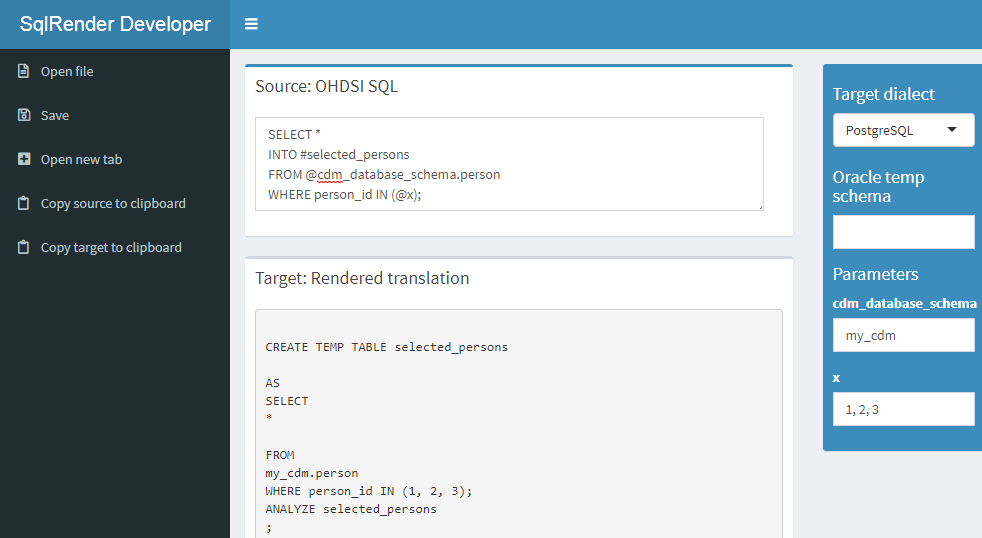
\includegraphics[width=1\linewidth]{images/SqlAndR/sqlDeveloper} 

}

\caption{The SqlDeveloper Shiny app.}\label{fig:sqlDeveloper}
\end{figure}

앱에서 OHDSI SQL을 입력하고 대상 언어를 선택하고 SQL에 매개 변수 값을
제공하면 자동으로 번역이 하단에 나타납니다.

\hypertarget{DatabaseConnector}{\section{DatabaseConnector}\label{DatabaseConnector}}

\href{https://ohdsi.github.io/DatabaseConnector/}{DatabaseConnector} 는
Java의 JDBC 드라이버를 사용하여 다양한 데이터베이스 플랫폼에
연결하기위한 R 패키지입니다. DatabaseConnector 패키지는 CRAN (종합 R
아카이브 네트워크)에서 사용할 수 있으므로 다음을 사용하여 설치할 수
있습니다:

\begin{Shaded}
\begin{Highlighting}[]
\KeywordTok{install.packages}\NormalTok{(}\StringTok{"DatabaseConnector"}\NormalTok{)}
\end{Highlighting}
\end{Shaded}

DatabaseConnector는 기존 데이터베이스 시스템(PostgreSQL, Microsoft SQL
Server, SQLite 및 Oracle), 병렬 데이터웨어 하우스(Microsoft APS, IBM
Netezza 및 Amazon RedShift) 및 빅데이터 플랫폼(Hadoop through Impla 및
Google BigQuery)을 포함한 다양한 기술 플랫폼을 지원합니다. 패키지에는
이미 대부분의 드라이버가 포함되어 있지만 라이선스 문제로 인해 BigQuery,
Netezza 및 Impla 용 드라이버는 포함되어 있지 않아서 사용자가 획득해야
합니다. 이러한 드라이버를 다운로드하는 방법에 대한 지침을 보려면
\texttt{?jdbcDrivers} 를 입력합니다. 다운로드한 후 \texttt{connect},
\texttt{dbConnect}, and \texttt{createConnectionDetails} 함수의
\texttt{pathToDriver} 인수로 사용할 수 있습니다.

\subsection{Creating a Connection}\label{creating-a-connection}

데이터베이스에 연결하려면 데이터베이스 플랫폼, 서버의 위치, 사용자 이름
및 비밀번호와 같은 많은 세부 사항을 지정해야 합니다. \texttt{connect}
함수를 호출하여 다음 세부 사항을 직접 지정할 수 있습니다:
\index{DatabaseConnector!creating a connection}

\begin{Shaded}
\begin{Highlighting}[]
\NormalTok{conn <-}\StringTok{ }\KeywordTok{connect}\NormalTok{(}\DataTypeTok{dbms =} \StringTok{"postgresql"}\NormalTok{,}
                \DataTypeTok{server =} \StringTok{"localhost/postgres"}\NormalTok{,}
                \DataTypeTok{user =} \StringTok{"joe"}\NormalTok{,}
                \DataTypeTok{password =} \StringTok{"secret"}\NormalTok{,}
                \DataTypeTok{schema =} \StringTok{"cdm"}\NormalTok{)}
\end{Highlighting}
\end{Shaded}

\begin{verbatim}
## Connecting using PostgreSQL driver
\end{verbatim}

각 플랫폼에 필요한 세부 사항에 대한 정보는 \texttt{?connect} 를
참조하십시오. 나중에 연결을 끊는 것을 잊지 마십시오:

\begin{Shaded}
\begin{Highlighting}[]
\KeywordTok{disconnect}\NormalTok{(conn)}
\end{Highlighting}
\end{Shaded}

서버이름을 제공하는 대신 JDBC connecting string을 사용하는 것이 더
편리할 경우 이를 제공할 수도 있다는 점에 유의하십시오:

\begin{Shaded}
\begin{Highlighting}[]
\NormalTok{connString <-}\StringTok{ "jdbc:postgresql://localhost:5432/postgres"}
\NormalTok{conn <-}\StringTok{ }\KeywordTok{connect}\NormalTok{(}\DataTypeTok{dbms =} \StringTok{"postgresql"}\NormalTok{,}
                \DataTypeTok{connectionString =}\NormalTok{ connString,}
                \DataTypeTok{user =} \StringTok{"joe"}\NormalTok{,}
                \DataTypeTok{password =} \StringTok{"secret"}\NormalTok{,}
                \DataTypeTok{schema =} \StringTok{"cdm"}\NormalTok{)}
\end{Highlighting}
\end{Shaded}

\begin{verbatim}
## Connecting using PostgreSQL driver
\end{verbatim}

때때로 우리는 먼저 세부 사항을 지정하고 나중에 연결할 때까지 연결을
연기해야 할 수 있습니다. 예를 들어 함수 내에서 연결이 설정되고 세부
사항은 인수로 전달해야 하는 경우 편리할 수 있습니다. 이 목적으로
\texttt{createConnectionDetails} 함수를 사용할 수 있습니다:

\begin{Shaded}
\begin{Highlighting}[]
\NormalTok{details <-}\StringTok{ }\KeywordTok{createConnectionDetails}\NormalTok{(}\DataTypeTok{dbms =} \StringTok{"postgresql"}\NormalTok{,}
                                   \DataTypeTok{server =} \StringTok{"localhost/postgres"}\NormalTok{,}
                                   \DataTypeTok{user =} \StringTok{"joe"}\NormalTok{,}
                                   \DataTypeTok{password =} \StringTok{"secret"}\NormalTok{,}
                                   \DataTypeTok{schema =} \StringTok{"cdm"}\NormalTok{)}
\NormalTok{conn <-}\StringTok{ }\KeywordTok{connect}\NormalTok{(details)}
\end{Highlighting}
\end{Shaded}

\begin{verbatim}
## Connecting using PostgreSQL driver
\end{verbatim}

\subsection{Querying}\label{querying}

데이터베이스 질의를 위한 주요 함수는 \texttt{querySql}과
\texttt{executeSql} functions. 입니다. 이러한 함수의 차이점은
\texttt{querySql}은 데이터베이스가 데이터를 반환할 것으로 예상하며,
한번에 하나의 SQL문만 처리할 수 있다는 것입니다. 이와 대조적으로
\texttt{executeSql}은 데이터를 반환할 것을 예상하지 않으며, 단일 SQL
문자열에서 복수의 SQL 문을 수용합니다.
\index{DatabaseConnector!querying}

Some examples:

\begin{Shaded}
\begin{Highlighting}[]
\KeywordTok{querySql}\NormalTok{(conn, }\StringTok{"SELECT TOP 3 * FROM person"}\NormalTok{)}
\end{Highlighting}
\end{Shaded}

\begin{verbatim}
##   person_id gender_concept_id year_of_birth
## 1         1              8507          1975
## 2         2              8507          1976
## 3         3              8507          1977
\end{verbatim}

\begin{Shaded}
\begin{Highlighting}[]
\KeywordTok{executeSql}\NormalTok{(conn, }\StringTok{"TRUNCATE TABLE foo; DROP TABLE foo;"}\NormalTok{)}
\end{Highlighting}
\end{Shaded}

두 함수 모두 광범위한 오류보고 기능을 제공합니다: 서버에서 오류가
발생하면 오류 메시지와 문제가 되는 SQL 부분이 텍스트 파일에 기록되어 더
나은 디버깅을 허용합니다. 기본적으로 \texttt{executeSql} 함수도 실행 된
SQL 문의 백분율을 나타내는 진행 표시 줄을 보여줍니다. 이러한 속성이
필요하지 않은 경우 패키지는 \texttt{lowLevelQuerySql}과
\texttt{lowLevelExecuteSql} 함수도 제공합니다.

\subsection{Querying Using Ffdf
Objects}\label{querying-using-ffdf-objects}

데이터베이스에서 가져올 데이터가 너무 커서 종종 메모리에 들어갈 수 없는
경우도 있습니다. \ref{BigDataSupport}, 절에서 언급했듯이, 그러한 경우
\texttt{ff} 패키지를 사용하여 R 데이터 객체를 파일에 저장하고 메모리에서
사용할 수 있는 것처럼 사용할 수 있습니다. \texttt{DatabaseConnector}는
객체에 데이터를 직접 다운로드 할 수 있습니다:

\begin{Shaded}
\begin{Highlighting}[]
\NormalTok{x <-}\StringTok{ }\KeywordTok{querySql.ffdf}\NormalTok{(conn, }\StringTok{"SELECT * FROM person"}\NormalTok{)}
\end{Highlighting}
\end{Shaded}

x는 이제 ffdf 객체입니다.

\subsection{Querying Different Platforms Using the Same
SQL}\label{querying-different-platforms-using-the-same-sql}

SqlRender 패키지의 \texttt{render} 및 \texttt{translate} 함수를 먼저
호출하는 다음과 같은 편의 함수를 사용할 수 있습니다:
\texttt{renderTranslateExecuteSql}, \texttt{renderTranslateQuerySql},
\texttt{renderTranslateQuerySql.ffdf}. 예를 들면:

\begin{Shaded}
\begin{Highlighting}[]
\NormalTok{x <-}\StringTok{ }\KeywordTok{renderTranslateQuerySql}\NormalTok{(conn, }
                             \DataTypeTok{sql =} \StringTok{"SELECT TOP 10 * FROM @schema.person"}\NormalTok{,}
                             \DataTypeTok{schema =} \StringTok{"cdm_synpuf"}\NormalTok{)}
\end{Highlighting}
\end{Shaded}

SQL Server 관련 `TOP 10' 구문은 PostgreSQL에서 예를 들어 `LIMIT 10'으로
변환되며 SQL 매개변수 \texttt{@schema} 는 제공된 값 `cdm\_synpuf'로
인스턴스화 되는 것에 주의해야합니다.

\subsection{Inserting Tables}\label{inserting-tables}

\texttt{executeSql} 함수를 사용하여 SQL 문을 전송하여 데이터베이스에
데이터를 삽입할 수도 있지만, \texttt{insertTable} 함수를 사용하는 것이
더 편리하고 빠릅니다(일부 최적화로 인해):

\begin{Shaded}
\begin{Highlighting}[]
\KeywordTok{data}\NormalTok{(mtcars)}
\KeywordTok{insertTable}\NormalTok{(conn, }\StringTok{"mtcars"}\NormalTok{, mtcars, }\DataTypeTok{createTable =} \OtherTok{TRUE}\NormalTok{)}
\end{Highlighting}
\end{Shaded}

이 예는 mtcars 데이터 프레임을 자동으로 서버의 'mtcars'라는 테이블로
업로드하고 생성합니다.

\section{Querying the CDM}\label{QueryTheCdm}

다음 예에서는 CDM이 적용된 데이터베이스를 질의하기 위해 OHDSI SQL을
사용합니다. 이러한 쿼리는 CDM의 데이터를 찾을 수 있는 데이터베이스
스키마를 나타내기 위해 \texttt{@cdm}을 사용합니다.

데이터베이스에 얼마나 많은 사람이 있는지 질의하는 것부터 시작할 수
있습니다:

\begin{Shaded}
\begin{Highlighting}[]
\KeywordTok{SELECT} \FunctionTok{COUNT}\NormalTok{(*) }\KeywordTok{AS}\NormalTok{ person_count }\KeywordTok{FROM}\NormalTok{ @cdm.person;}
\end{Highlighting}
\end{Shaded}

\begin{longtable}[]{@{}r@{}}
\toprule
PERSON\_COUNT\tabularnewline
\midrule
\endhead
26299001\tabularnewline
\bottomrule
\end{longtable}

아니면 observation period의 평균에 관심이 있을 수도 있습니다:

\begin{Shaded}
\begin{Highlighting}[]
\KeywordTok{SELECT} \FunctionTok{AVG}\NormalTok{(DATEDIFF(}\DataTypeTok{DAY}\NormalTok{, }
\NormalTok{                    observation_period_start_date, }
\NormalTok{                    observation_period_end_date) / }\FloatTok{365.25}\NormalTok{) }\KeywordTok{AS}\NormalTok{ num_years}
\KeywordTok{FROM}\NormalTok{ @cdm.observation_period;}
\end{Highlighting}
\end{Shaded}

\begin{longtable}[]{@{}r@{}}
\toprule
NUM\_YEARS\tabularnewline
\midrule
\endhead
1.980803\tabularnewline
\bottomrule
\end{longtable}

테이블을 조인하여 추가 통계를 생성할 수 있습니다. 조인은 일반적으로
테이블의 특정 필드가 동일한 값을 갖도록 하여 여러 테이블의 필드를
결합합니다. 예를 들어 여기서 두 테이블 모두 가지고 있는 PERSON\_ID
필드로 PERSON 테이블과 OBSERVATION\_PEROPD 테이블을 조인합니다. 즉,
조인의 결과는 두 테이블의 모든 필드를 갖는 새로운 테이블과 같은
집합이지만, 모든 행에서 두테이블의 PERSON\_ID는 동일한 값을
가져야합니다. 예를 들어 PERSON 테이블의 YEAR\_OF\_BIRTH 필드와 함께
OBSERVATION\_PERIOD 테이블의 OBSERVATION\_PERIOD\_END\_DATE 필드를
사용하여 관찰 종료 최대 연력을 계산할 수 있습니다:

\begin{Shaded}
\begin{Highlighting}[]
\KeywordTok{SELECT} \FunctionTok{MAX}\NormalTok{(}\DataTypeTok{YEAR}\NormalTok{(observation_period_end_date) -}
\NormalTok{           year_of_birth) }\KeywordTok{AS}\NormalTok{ max_age}
\KeywordTok{FROM}\NormalTok{ @cdm.person}
\KeywordTok{INNER} \KeywordTok{JOIN}\NormalTok{ @cdm.observation_period}
  \KeywordTok{ON}\NormalTok{ person.person_id = observation_period.person_id;}
\end{Highlighting}
\end{Shaded}

\begin{longtable}[]{@{}r@{}}
\toprule
MAX\_AGE\tabularnewline
\midrule
\endhead
90\tabularnewline
\bottomrule
\end{longtable}

관찰 시작 당시시연령 분포를 결정하려면 훨씬 더 복잡한 질의가 필요합니다.
이 질의에서는 먼저 PERSON 테이블과 OBSERVATION\_PERIOD을 조인하여 관찰
당시 연령을 계산합니다. 또한 연령을 기준으로 이 조인된 집합의 순서를
정렬하고 order\_nr로 저장합니다. 이 조인의 결과를 여러 번 사용하고 싶기
때문에 ``ages''라고 하는 common table expression (CTE)
(\texttt{WITH\ ...\ AS}를 사용하여 정의된) 으로 정의한다. 즉, 연령을
기존 테이블인 것처럼 나타낼 수 있습니다. ``ages''의 행 수를 세어 ``n''을
생성하고 각 사분위수에 대해 order\_nr이 분수 시간 ``n,'' 보다 작은 최소
연령을 찾습니다. 예를 들어, 중앙값을 찾기 위해 \(order\_nr < .50 * n\)인
최소 연령을 사용합니다. 최소 및 최대 연령은 별도로 계산됩니다:

\begin{Shaded}
\begin{Highlighting}[]
\KeywordTok{WITH}\NormalTok{ ages}
\KeywordTok{AS}\NormalTok{ (}
    \KeywordTok{SELECT}\NormalTok{ age,}
        \FunctionTok{ROW_NUMBER}\NormalTok{() }\KeywordTok{OVER}\NormalTok{ (}
            \KeywordTok{ORDER} \KeywordTok{BY}\NormalTok{ age}
\NormalTok{            ) order_nr}
    \KeywordTok{FROM}\NormalTok{ (}
        \KeywordTok{SELECT} \DataTypeTok{YEAR}\NormalTok{(observation_period_start_date) - year_of_birth }\KeywordTok{AS}\NormalTok{ age}
        \KeywordTok{FROM}\NormalTok{ @cdm.person}
        \KeywordTok{INNER} \KeywordTok{JOIN}\NormalTok{ @cdm.observation_period}
            \KeywordTok{ON}\NormalTok{ person.person_id = observation_period.person_id}
\NormalTok{        ) age_computed}
\NormalTok{    )}
\KeywordTok{SELECT} \FunctionTok{MIN}\NormalTok{(age) }\KeywordTok{AS}\NormalTok{ min_age,}
    \FunctionTok{MIN}\NormalTok{(}\KeywordTok{CASE} 
            \KeywordTok{WHEN}\NormalTok{ order_nr < .}\DecValTok{25}\NormalTok{ * n}
                \KeywordTok{THEN} \DecValTok{9999}
            \KeywordTok{ELSE}\NormalTok{ age}
            \KeywordTok{END}\NormalTok{) }\KeywordTok{AS}\NormalTok{ q25_age,}
    \FunctionTok{MIN}\NormalTok{(}\KeywordTok{CASE} 
            \KeywordTok{WHEN}\NormalTok{ order_nr < .}\DecValTok{50}\NormalTok{ * n}
                \KeywordTok{THEN} \DecValTok{9999}
            \KeywordTok{ELSE}\NormalTok{ age}
            \KeywordTok{END}\NormalTok{) }\KeywordTok{AS}\NormalTok{ median_age,}
    \FunctionTok{MIN}\NormalTok{(}\KeywordTok{CASE} 
            \KeywordTok{WHEN}\NormalTok{ order_nr < .}\DecValTok{75}\NormalTok{ * n}
                \KeywordTok{THEN} \DecValTok{9999}
            \KeywordTok{ELSE}\NormalTok{ age}
            \KeywordTok{END}\NormalTok{) }\KeywordTok{AS}\NormalTok{ q75_age,}
    \FunctionTok{MAX}\NormalTok{(age) }\KeywordTok{AS}\NormalTok{ max_age}
\KeywordTok{FROM}\NormalTok{ ages}
\KeywordTok{CROSS} \KeywordTok{JOIN}\NormalTok{ (}
    \KeywordTok{SELECT} \FunctionTok{COUNT}\NormalTok{(*) }\KeywordTok{AS}\NormalTok{ n}
    \KeywordTok{FROM}\NormalTok{ ages}
\NormalTok{    ) population_size;}
\end{Highlighting}
\end{Shaded}

\begin{longtable}[]{@{}rrrrr@{}}
\toprule
MIN\_AGE & Q25\_AGE & MEDIAN\_AGE & Q75\_AGE & MAX\_AGE\tabularnewline
\midrule
\endhead
0 & 6 & 17 & 34 & 90\tabularnewline
\bottomrule
\end{longtable}

SQL을 사용하는 대신 R에서 더 복잡한 계산을 수행할 수도 있습니다. 예를
들어, 이 코드를 사용하여 동일한 결과를 얻을 수 있습니다:

\begin{Shaded}
\begin{Highlighting}[]
\NormalTok{sql <-}\StringTok{ "SELECT YEAR(observation_period_start_date) -}
\StringTok{               year_of_birth AS age}
\StringTok{FROM @cdm.person}
\StringTok{INNER JOIN @cdm.observation_period}
\StringTok{  ON person.person_id = observation_period.person_id;"}
\NormalTok{age <-}\StringTok{ }\KeywordTok{renderTranslateQuerySql}\NormalTok{(conn, sql, }\DataTypeTok{cdm =} \StringTok{"cdm"}\NormalTok{)}
\KeywordTok{quantile}\NormalTok{(age[, }\DecValTok{1}\NormalTok{], }\KeywordTok{c}\NormalTok{(}\DecValTok{0}\NormalTok{, }\FloatTok{0.25}\NormalTok{, }\FloatTok{0.5}\NormalTok{, }\FloatTok{0.75}\NormalTok{, }\DecValTok{1}\NormalTok{))}
\end{Highlighting}
\end{Shaded}

\begin{verbatim}
##   0%  25%  50%  75% 100% 
##    0    6   17   34   90
\end{verbatim}

서버에서 연령을 계산하고 모든 연령들을 다운로드한 다음 연령 분포를
계산합니다. 그러나 이를 위해서는 데이터베이스 서버에서 수백만 행의
데이터를 다운로드해야 하므로 효율성이 떨어집니다. 계산이 SQL에서 가장 잘
수행되는지 R에서 가장 잘 수행되는지 여부를 사례별로 결정해야합니다.

질의는 CDM의 source value를 사용할 수 있습니다. 예를 들어, 다음을
사용하여 가장 빈번한 상위 10개의 condition source code를 검색할 수
있습니다:

\begin{Shaded}
\begin{Highlighting}[]
\KeywordTok{SELECT}\NormalTok{ TOP }\DecValTok{10}\NormalTok{ condition_source_value, }
  \FunctionTok{COUNT}\NormalTok{(*) }\KeywordTok{AS}\NormalTok{ code_count}
\KeywordTok{FROM}\NormalTok{ @cdm.condition_occurrence}
\KeywordTok{GROUP} \KeywordTok{BY}\NormalTok{ condition_source_value}
\KeywordTok{ORDER} \KeywordTok{BY}\NormalTok{ -COUNT(*);}
\end{Highlighting}
\end{Shaded}

\begin{longtable}[]{@{}rr@{}}
\toprule
CONDITION\_SOURCE\_VALUE & CODE\_COUNT\tabularnewline
\midrule
\endhead
4019 & 49094668\tabularnewline
25000 & 36149139\tabularnewline
78099 & 28908399\tabularnewline
319 & 25798284\tabularnewline
31401 & 22547122\tabularnewline
317 & 22453999\tabularnewline
311 & 19626574\tabularnewline
496 & 19570098\tabularnewline
I10 & 19453451\tabularnewline
3180 & 18973883\tabularnewline
\bottomrule
\end{longtable}

여기서 CONDITION\_OCCURRENCE 테이블의 행을 CONDITION\_SOURCE\_VALUE
필드의 값으로 그룹화하고 각 그룹의 행 수를 세었습니다.

\section{Using the Vocabulary When
Querying}\label{using-the-vocabulary-when-querying}

많은 작업에서 Vocabulary는 유용합니다. Vocabulary 테이블은 CDM의
일부이므로 SQL 쿼리를 사용하여 이용할 수 있습니다. Vocabulary에 대한
질의가 CDM에 대한 질의와 어떻게 결합될 수 있는지 보여줍니다. CDM의 많은
필드에는 CONCEPT 테이블을 사용하여 확인할 수 있는 concept ID들을
포함되어 있습니다. 예를 들어, 성별에 따라 계층화된 데이터베이스의
인원수를 셀 수 있고. GENDER\_CONCEPT\_ID를 concept name으로 해결하는
것이 편리할 것입니다:

\begin{Shaded}
\begin{Highlighting}[]
\KeywordTok{SELECT} \FunctionTok{COUNT}\NormalTok{(*) }\KeywordTok{AS}\NormalTok{ subject_count,}
\NormalTok{  concept_name}
\KeywordTok{FROM}\NormalTok{ @cdm.person}
\KeywordTok{INNER} \KeywordTok{JOIN}\NormalTok{ @cdm.concept}
  \KeywordTok{ON}\NormalTok{ person.gender_concept_id = concept.concept_id}
\KeywordTok{GROUP} \KeywordTok{BY}\NormalTok{ concept_name;}
\end{Highlighting}
\end{Shaded}

\begin{longtable}[]{@{}rr@{}}
\toprule
SUBJECT\_COUNT & CONCEPT\_NAME\tabularnewline
\midrule
\endhead
14927548 & FEMALE\tabularnewline
11371453 & MALE\tabularnewline
\bottomrule
\end{longtable}

Vocabulary의 매우 강력한 특징은 계층입니다. 매우 일반적인 질의는 특정
개념과 \emph{모든 하위 개념}을 찾습니다. 예를 들어, ibuprofen 성분이
들어있는 처방전의 수를 세고 싶다고 상상해보십시오:

\begin{Shaded}
\begin{Highlighting}[]
\KeywordTok{SELECT} \FunctionTok{COUNT}\NormalTok{(*) }\KeywordTok{AS}\NormalTok{ prescription_count}
\KeywordTok{FROM}\NormalTok{ @cdm.drug_exposure}
\KeywordTok{INNER} \KeywordTok{JOIN}\NormalTok{ @cdm.concept_ancestor}
  \KeywordTok{ON}\NormalTok{ drug_concept_id = descendant_concept_id}
\KeywordTok{INNER} \KeywordTok{JOIN}\NormalTok{ @cdm.concept ingredient}
  \KeywordTok{ON}\NormalTok{ ancestor_concept_id = ingredient.concept_id}
\KeywordTok{WHERE} \FunctionTok{LOWER}\NormalTok{(ingredient.concept_name) = }\StringTok{'ibuprofen'}
  \KeywordTok{AND}\NormalTok{ ingredient.concept_class_id = }\StringTok{'Ingredient'}
  \KeywordTok{AND}\NormalTok{ ingredient.standard_concept = }\StringTok{'S'}\NormalTok{;}
\end{Highlighting}
\end{Shaded}

\begin{longtable}[]{@{}r@{}}
\toprule
PRESCRIPTION\_COUNT\tabularnewline
\midrule
\endhead
26871214\tabularnewline
\bottomrule
\end{longtable}

\section{QueryLibrary}\label{querylibrary}

\index{QueryLibrary}

QueryLibrary는 CDM에 대해 일반적으로 사용되는 SQL 질의들의
라이브러리입니다. 그림 \ref{fig:queryLibrary}에 표시된 응용
프로그램\footnote{\url{http://data.ohdsi.org/QueryLibrary}} 및 R
패키지로 제공됩니다.\footnote{\url{https://github.com/OHDSI/QueryLibrary}}

\begin{figure}

{\centering 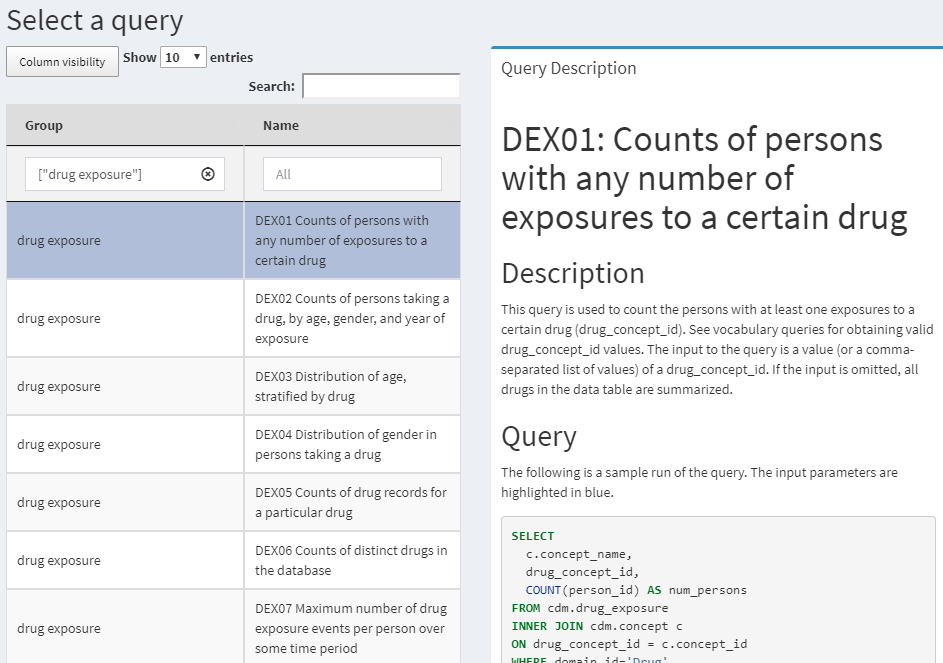
\includegraphics[width=1\linewidth]{images/SqlAndR/queryLibrary} 

}

\caption{QueryLibrary: a library of SQL queries against the CDM.}\label{fig:queryLibrary}
\end{figure}

라이브러리의 목적은 새로운 사용자가 CDM에 질의하는 방법을 배우도록 돕는
것입니다. 라이브러리의 질의는 OHDSI 커뮤니티에서 검토하고 승인했습니다.
질의 라이브러리는 주로 교육 목적으로 사용되지만 숙련된 사용자에게 유용한
자원이기도 합니다,

QueryLibrary는 SqlRender를 사용하여 선택한 SQL 언어로 질의를 출력합니다.
사용자는 CDM 데이터베이스 스키마, vocabulary 데이터베이스 스키마(별도의
경우) 및 Oracle 임시 스키마(필요한 경우)를 지정할 수 있으므로 이러한
설정으로 질의가 자동으로 랜더링 됩니다.

\section{Designing a Simple Study}\label{designing-a-simple-study}

\subsection{Problem Definition}\label{problem-definition}

Angioedema (혈관 부종)은 ACE inhibitor (ACEi)의 잘 알려진 부작용입니다.
\citet{slater_1988} ACEi 치료 첫 주에 혈관 부종의 발생률이 주당 3,000
명의 환자 당 1건인 것으로 추정했습니다. 여기서 우리는 이 결론을 모방하고
연령과 성별에 따라 계층화합니다. 간단하게 하기 위해서 우리는 하나의
ACEi: lisinopril에 중점을 둡니다. 따라서 우리는 질문에 대답합니다.

\begin{quote}
Lisinopril 치료 개시 후 첫 주에 연령과 성별에 따라 계층화되는 혈관
부종의 비율은 얼마입니까?
\end{quote}

\subsection{Exposure}\label{exposure}

Exposure (노출)은 lisinopril에 대한 첫번째 노출로 정의합니다. 먼저
이전에 lisinopril에 노출되지 않았음을 의미합니다. 첫 노출 전에 365 일의
연속 관찰 기간이 필요합니다.

\subsection{Outcome}\label{outcome}

입원 또는 응급실 방문 중 혈관 부종 진단 코드의 발생으로 혈관 부종을
정의합니다.

\subsection{Time-At-Risk}\label{time-at-risk}

환자가 일주일 동안 노출되었는지 여부에 관계없이 이 치료 시작 후 첫 주에
발생률을 계산합니다.

\section{Implementing the Study Using SQL and
R}\label{implementing-the-study-using-sql-and-r}

OHDSI 툴 규약에 구속되지 않지만 동일한 원칙을 따르는 것은 도움이 됩니다.
이 경우 OHDSI 툴의 작동 방식과 유사하게 SQL을 사용하여 cohort(코호트)
테이블을 채웁니다. 코호트 테이블은 CDM에 정의되어 있으며 사전 정의된
필드 집합도 있습니다. 먼저 쓰기 접근 권한이 있는 데이터베이스 스키마에
COHORT 테이블을 만들어야 하는데, 이는 CDM 형식으로 데이터를 저장하는
데이터베이스 스키마와 동일하지 않을 수 있습니다.

\begin{Shaded}
\begin{Highlighting}[]
\KeywordTok{library}\NormalTok{(DatabaseConnector)}
\NormalTok{conn <-}\StringTok{ }\KeywordTok{connect}\NormalTok{(}\DataTypeTok{dbms =} \StringTok{"postgresql"}\NormalTok{,}
                \DataTypeTok{server =} \StringTok{"localhost/postgres"}\NormalTok{,}
                \DataTypeTok{user =} \StringTok{"joe"}\NormalTok{,}
                \DataTypeTok{password =} \StringTok{"secret"}\NormalTok{)}
\NormalTok{cdmDbSchema <-}\StringTok{ "cdm"}
\NormalTok{cohortDbSchema <-}\StringTok{ "scratch"}
\NormalTok{cohortTable <-}\StringTok{ "my_cohorts"}

\NormalTok{sql <-}\StringTok{ "}
\StringTok{CREATE TABLE @cohort_db_schema.@cohort_table (}
\StringTok{  cohort_definition_id INT,}
\StringTok{  cohort_start_date DATE,}
\StringTok{  cohort_end_date DATE,}
\StringTok{  subject_id BIGINT}
\StringTok{);}
\StringTok{"}
\KeywordTok{renderTranslateExecuteSql}\NormalTok{(conn, sql,}
                          \DataTypeTok{cohort_db_schema =}\NormalTok{ cohortDbSchema,}
                          \DataTypeTok{cohort_table =}\NormalTok{ cohortTable)}
\end{Highlighting}
\end{Shaded}

여기서는 데이터베이스 스키마 및 테이블 이름을 매개 변수화 하여 다른
환경에 쉽게 적용할 수 있습니다. 결과는 데이터베이스 서버의 빈
테이블입니다.

\subsection{Exposure Cohort}\label{exposure-cohort}

다음으로 노출 코호트를 만들어 COHORT 테이블에 삽입합니다:

\begin{Shaded}
\begin{Highlighting}[]
\NormalTok{sql <-}\StringTok{ "}
\StringTok{INSERT INTO @cohort_db_schema.@cohort_table (}
\StringTok{  cohort_definition_id,}
\StringTok{  cohort_start_date,}
\StringTok{  cohort_end_date,}
\StringTok{  subject_id}
\StringTok{)}
\StringTok{SELECT 1 AS cohort_definition_id,}
\StringTok{  cohort_start_date,}
\StringTok{  cohort_end_date,}
\StringTok{  subject_id}
\StringTok{FROM (}
\StringTok{  SELECT drug_era_start_date AS cohort_start_date,}
\StringTok{    drug_era_end_date AS cohort_end_date,}
\StringTok{    person_id AS subject_id}
\StringTok{  FROM (}
\StringTok{    SELECT drug_era_start_date,}
\StringTok{      drug_era_end_date,}
\StringTok{      person_id,}
\StringTok{      ROW_NUMBER() OVER (}
\StringTok{        PARTITION BY person_id}
\StringTok{            ORDER BY drug_era_start_date}
\StringTok{      ) order_nr}
\StringTok{    FROM @cdm_db_schema.drug_era}
\StringTok{    WHERE drug_concept_id = 1308216 -- Lisinopril}
\StringTok{  ) ordered_exposures}
\StringTok{  WHERE order_nr = 1}
\StringTok{) first_era}
\StringTok{INNER JOIN @cdm_db_schema.observation_period}
\StringTok{  ON subject_id = person_id}
\StringTok{    AND observation_period_start_date < cohort_start_date}
\StringTok{    AND observation_period_end_date > cohort_start_date}
\StringTok{WHERE DATEDIFF(DAY,}
\StringTok{               observation_period_start_date,}
\StringTok{               cohort_start_date) >= 365;}
\StringTok{"}

\KeywordTok{renderTranslateExecuteSql}\NormalTok{(conn, sql,}
                          \DataTypeTok{cohort_db_schema =}\NormalTok{ cohortDbSchema,}
                          \DataTypeTok{cohort_table =}\NormalTok{ cohortTable,}
                          \DataTypeTok{cdm_db_schema =}\NormalTok{ cdmDbSchema)}
\end{Highlighting}
\end{Shaded}

여기에서는 DRUG\_EXPOSURE 테이블에서 자동으로 파생되는 CDM의 표준
테이블인 DRUG ERA 테이블을 사용합니다. DRUG ERA 테이블에는 성분 수준에서
연속 노출 기간이 포함되어 있습니다. 따라서 lisinopril을 검색할 수
있으며, 이는 lisinopril을 함유 한 약물에 대한 모든 노출을 자동으로
식별합니다. 사람당 첫 번째 약물 노출을 취한 다음 OBSERVATION\_PERIOD
테이블과 조인하고 한 사람이 여러 관찰 기간을 가질 수 있으므로 약물
노출이 포함된 기간에만 조인해야 합니다. 그런 다음
OBSERVATION\_PERIOD\_START\_DATE와 COHORT\_START\_DATE 사이에 적어도
365일이 필요합니다.

\subsection{Outcome Cohort}\label{outcome-cohort}

마지막으로, 우리는 outcome (결과) 코호트를 만들어야 합니다:

\begin{Shaded}
\begin{Highlighting}[]
\NormalTok{sql <-}\StringTok{ "}
\StringTok{INSERT INTO @cohort_db_schema.@cohort_table (}
\StringTok{ cohort_definition_id,}
\StringTok{ cohort_start_date,}
\StringTok{ cohort_end_date,}
\StringTok{subject_id}
\StringTok{)}
\StringTok{SELECT 2 AS cohort_definition_id,}
\StringTok{  cohort_start_date,}
\StringTok{  cohort_end_date,}
\StringTok{  subject_id}
\StringTok{FROM (}
\StringTok{  SELECT DISTINCT person_id AS subject_id,}
\StringTok{    condition_start_date AS cohort_start_date,}
\StringTok{    condition_end_date AS cohort_end_date}
\StringTok{  FROM @cdm_db_schema.condition_occurrence}
\StringTok{  INNER JOIN @cdm_db_schema.concept_ancestor}
\StringTok{    ON condition_concept_id = descendant_concept_id}
\StringTok{  WHERE ancestor_concept_id = 432791 -- Angioedema}
\StringTok{) distinct_occurrence}
\StringTok{INNER JOIN @cdm_db_schema.visit_occurrence}
\StringTok{  ON subject_id = person_id}
\StringTok{  AND visit_start_date <= cohort_start_date}
\StringTok{  AND visit_end_date >= cohort_start_date}
\StringTok{WHERE visit_concept_id IN (262, 9203,}
\StringTok{    9201) -- Inpatient or ER;}
\StringTok{"}

\KeywordTok{renderTranslateExecuteSql}\NormalTok{(conn, sql,}
                          \DataTypeTok{cohort_db_schema =}\NormalTok{ cohortDbSchema,}
                          \DataTypeTok{cohort_table =}\NormalTok{ cohortTable,}
                          \DataTypeTok{cdm_db_schema =}\NormalTok{ cdmDbSchema)}
\end{Highlighting}
\end{Shaded}

CONDITION OCCURRECE 테이블과 CONCEPT ANCESTOR 테이블을 조인하여 모든
혈관 부종과 그 자손을 찾습니다. 같은 날에 여러 혈관 부종의 진단이 여러
혈관 부종 발생이 아닌 동일한 사건 일 가능성이 높기 때문에 DISTINCT를
사용하여 하루에 하나의 행만 선택하도록 합니다. 이러한 발생을
VISIT\_OCCURRENCE 테이블과 조인하여 입원이나 응급실 환경에서
진단되었는지 확인합니다.

\subsection{Incidence Rate
Calculation}\label{incidence-rate-calculation}

코호트가 준비되었으므로 연령과 성별에 따라 계층화되는 발생률을 계산할 수
있습니다:

\begin{Shaded}
\begin{Highlighting}[]
\NormalTok{sql <-}\StringTok{ "}
\StringTok{WITH tar AS (}
\StringTok{  SELECT concept_name AS gender,}
\StringTok{    FLOOR((YEAR(cohort_start_date) -}
\StringTok{          year_of_birth) / 10) AS age,}
\StringTok{    subject_id,}
\StringTok{    cohort_start_date,}
\StringTok{    CASE WHEN DATEADD(DAY, 7, cohort_start_date) >}
\StringTok{      observation_period_end_date}
\StringTok{    THEN observation_period_end_date}
\StringTok{    ELSE DATEADD(DAY, 7, cohort_start_date)}
\StringTok{    END AS cohort_end_date}
\StringTok{  FROM @cohort_db_schema.@cohort_table}
\StringTok{  INNER JOIN @cdm_db_schema.observation_period}
\StringTok{    ON subject_id = observation_period.person_id}
\StringTok{      AND observation_period_start_date < cohort_start_date}
\StringTok{      AND observation_period_end_date > cohort_start_date}
\StringTok{  INNER JOIN @cdm_db_schema.person}
\StringTok{    ON subject_id = person.person_id}
\StringTok{  INNER JOIN @cdm_db_schema.concept}
\StringTok{    ON gender_concept_id = concept_id}
\StringTok{  WHERE cohort_definition_id = 1 -- Exposure}
\StringTok{)}
\StringTok{SELECT days.gender,}
\StringTok{    days.age,}
\StringTok{    days,}
\StringTok{    CASE WHEN events IS NULL THEN 0 ELSE events END AS events}
\StringTok{FROM (}
\StringTok{  SELECT gender,}
\StringTok{    age,}
\StringTok{    SUM(DATEDIFF(DAY, cohort_start_date,}
\StringTok{      cohort_end_date)) AS days}
\StringTok{  FROM tar}
\StringTok{  GROUP BY gender,}
\StringTok{    age}
\StringTok{) days}
\StringTok{LEFT JOIN (}
\StringTok{  SELECT gender,}
\StringTok{      age,}
\StringTok{      COUNT(*) AS events}
\StringTok{  FROM tar}
\StringTok{  INNER JOIN @cohort_db_schema.@cohort_table angioedema}
\StringTok{    ON tar.subject_id = angioedema.subject_id}
\StringTok{      AND tar.cohort_start_date <= angioedema.cohort_start_date}
\StringTok{      AND tar.cohort_end_date >= angioedema.cohort_start_date}
\StringTok{  WHERE cohort_definition_id = 2 -- Outcome}
\StringTok{  GROUP BY gender,}
\StringTok{    age}
\StringTok{) events}
\StringTok{ON days.gender = events.gender}
\StringTok{  AND days.age = events.age;}
\StringTok{"}

\NormalTok{results <-}\StringTok{ }\KeywordTok{renderTranslateQuerySql}\NormalTok{(conn, sql,}
                                   \DataTypeTok{cohort_db_schema =}\NormalTok{ cohortDbSchema,}
                                   \DataTypeTok{cohort_table =}\NormalTok{ cohortTable,}
                                   \DataTypeTok{cdm_db_schema =}\NormalTok{ cdmDbSchema,}
                                   \DataTypeTok{snakeCaseToCamelCase =} \OtherTok{TRUE}\NormalTok{)}
\end{Highlighting}
\end{Shaded}

우선 적절한 time-at-risk (위험 관찰 기간)로 모든 노출을 포함하는 CTE인
``tar''를 만듭니다. OBSERVATION\_PERIOD\_END\_DATE에서 위험 관찰 기간을
단축한다는 점에 유의합니다. 또한 10년 단위로 나이를 계산하고 성별을
파악합니다. CTE를 사용하면 동일한 중간 결과 집합을 질의에서 여러 번
사용할 수 있다는 장점이 있습니다. 이 경우 위험 관찰 기간동안 발생하는
혈관 부종 사건의 수와 총 위험 관찰 기간의 양을 계산하는데 사용됩니다.

SQL에서는 필드 이름에 snake\_case (대소문자를 구분하지 않는)를 사용하는
반면 R에서는 camelCase (대수문자를 구분하는)를 사용하는 경향이 있기 때문
\texttt{snakeCaseToCamelCase\ =\ TRUE}로 합니다. The \texttt{results}
데이터 프레임 열 이름은 이제 camelCase입니다.

ggplot 패키지의 도움 을 받아 다음과 같은 결과를 쉽게 표시할 수 있습니다:

\begin{Shaded}
\begin{Highlighting}[]
\CommentTok{# Compute incidence rate (IR) :}
\NormalTok{results}\OperatorTok{$}\NormalTok{ir <-}\StringTok{ }\DecValTok{1000} \OperatorTok{*}\StringTok{ }\NormalTok{results}\OperatorTok{$}\NormalTok{events }\OperatorTok{/}\StringTok{ }\NormalTok{results}\OperatorTok{$}\NormalTok{days }\OperatorTok{/}\StringTok{ }\DecValTok{7}

\CommentTok{# Fix age scale:}
\NormalTok{results}\OperatorTok{$}\NormalTok{age <-}\StringTok{ }\NormalTok{results}\OperatorTok{$}\NormalTok{age }\OperatorTok{*}\StringTok{ }\DecValTok{10}

\KeywordTok{library}\NormalTok{(ggplot2)}
\KeywordTok{ggplot}\NormalTok{(results, }\KeywordTok{aes}\NormalTok{(}\DataTypeTok{x =}\NormalTok{ age, }\DataTypeTok{y =}\NormalTok{ ir, }\DataTypeTok{group =}\NormalTok{ gender, }\DataTypeTok{color =}\NormalTok{ gender)) }\OperatorTok{+}
\StringTok{  }\KeywordTok{geom_line}\NormalTok{() }\OperatorTok{+}
\StringTok{  }\KeywordTok{xlab}\NormalTok{(}\StringTok{"Age"}\NormalTok{) }\OperatorTok{+}
\StringTok{  }\KeywordTok{ylab}\NormalTok{(}\StringTok{"Incidence (per 1,000 patient weeks)"}\NormalTok{)}
\end{Highlighting}
\end{Shaded}

\begin{center}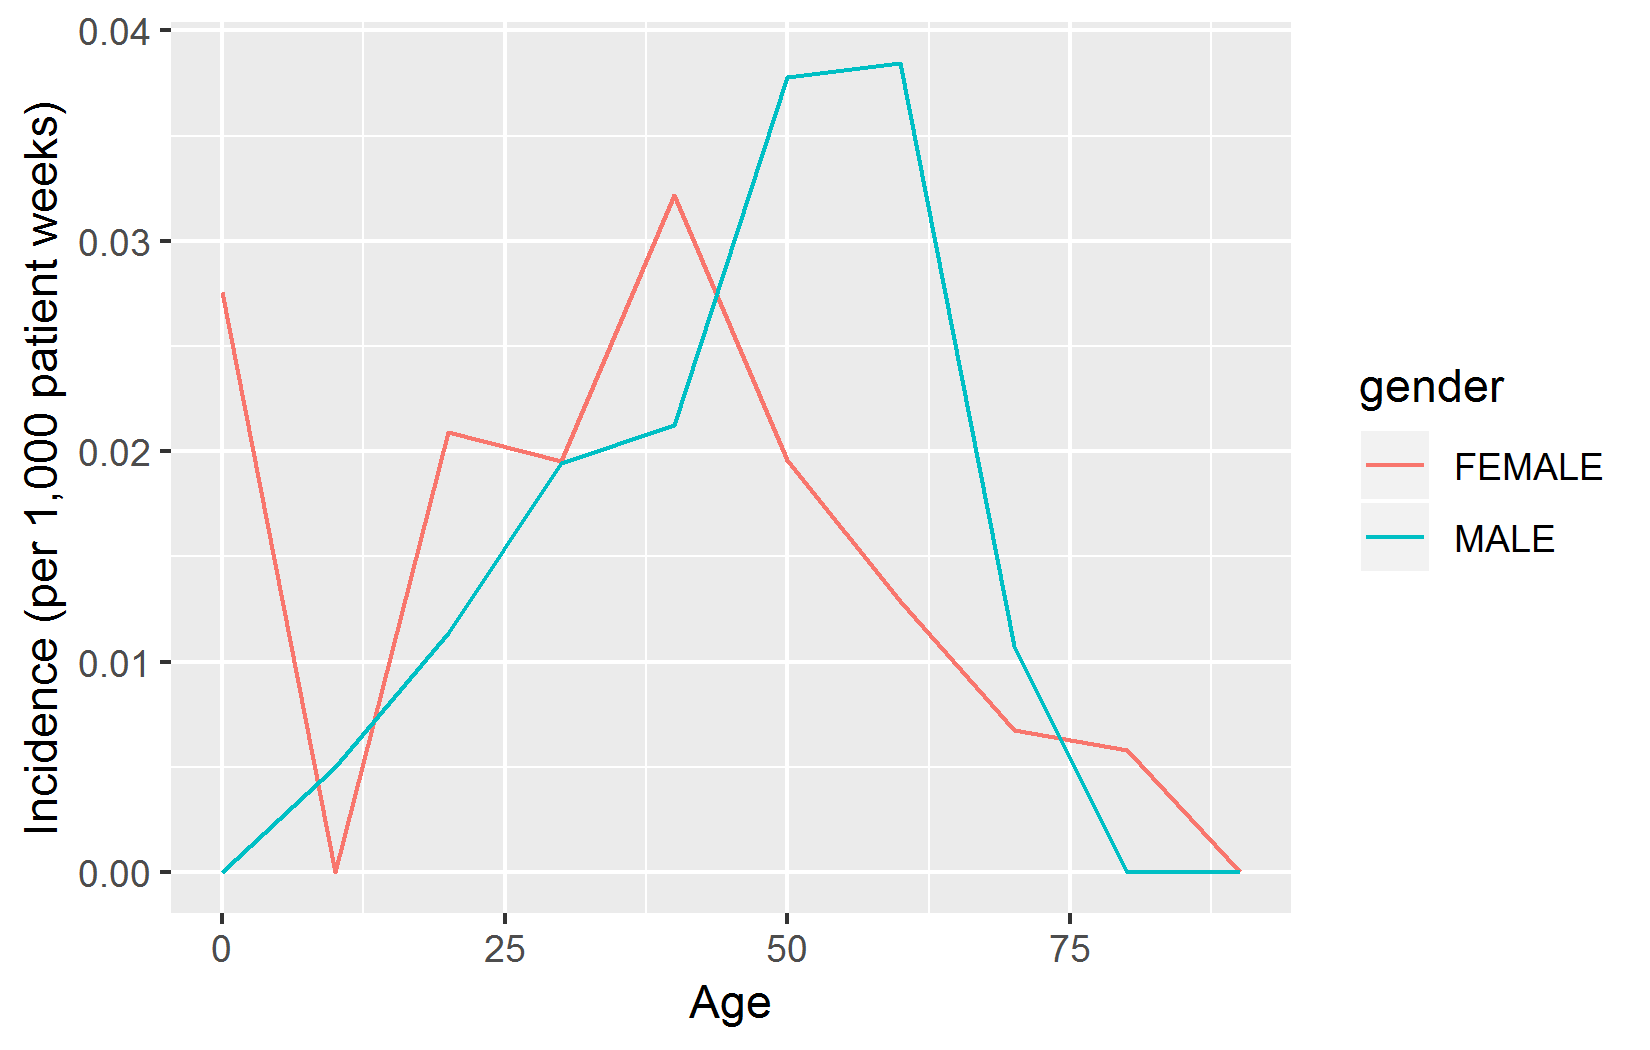
\includegraphics[width=0.8\linewidth]{images/SqlAndR/ir} \end{center}

\subsection{Clean Up}\label{clean-up}

생성한 테이블을 정리하고 연결을 닫는 것을 잊지 마십시오:

\begin{Shaded}
\begin{Highlighting}[]
\NormalTok{sql <-}\StringTok{ "}
\StringTok{TRUNCATE TABLE @cohort_db_schema.@cohort_table;}
\StringTok{DROP TABLE @cohort_db_schema.@cohort_table;}
\StringTok{"}
\KeywordTok{renderTranslateExecuteSql}\NormalTok{(conn, sql,}
                          \DataTypeTok{cohort_db_schema =}\NormalTok{ cohortDbSchema,}
                          \DataTypeTok{cohort_table =}\NormalTok{ cohortTable)}

\KeywordTok{disconnect}\NormalTok{(conn)}
\end{Highlighting}
\end{Shaded}

\subsection{Compatibility}\label{compatibility}

OHDSI SQL을 DatabaseConnector 및 SQLRender와 함께 사용하기 때문에 여기서
검토한 코드는 OHDSI가 지원하는 모든 데이터베이스 플랫폼에서 실행됩니다.

시연 목적으로 수작업으로 만든 SQL을 사용하여 코호트를 만들기로
결정했다는 점에 유의하십시오. ATLAS에서 코호트 정의를 구성하고 ATALS에서
생성된 SQL을 사용하여 코호트를 인스턴스화 하는 것이 더 편리했을
것입니다. ATLAS는 또한 OHDSI SQL을 생성하였고, 따라서 SqlRender 및
DatabaseConnector와 함께 쉽게 사용할 수 있습니다.

\section{Summary}\label{summary-3}

\BeginKnitrBlock{rmdsummary}
\begin{itemize}
\item
  \textbf{SQL}은 공통 데이터 모델을 따르는 데이터베이스를 포함하여
  데이터베이스를 조회하기위한 표준 언어입니다.
\item
  데이터베이스 플랫폼마다 SQL 언어가 다르며 이를 질의하기 위해서는 다른
  툴이 필요합니다.
\item
  \textbf{SqlRender} 및 \textbf{DatabaseConnector} R 패키지는 CDM에서
  데이터를 질의하는 통합된 방법을 제공하므로 동일한 분석 코드를 수정없이
  다른 환경에서 실행할 수 있습니다.
\item
  R과 SQL을 함께 사용하면 OHDSI 툴에서 지원하지 않는 사용자 맞춤 분석
  연구를 구현할 수 있습니다.
\item
  \textbf{QueryLibrary} 는 CDM에 재사용 가능한 SQL 질의 모음을
  제공합니다..
\end{itemize}
\EndKnitrBlock{rmdsummary}

\section{Exercises}\label{exercises-1}

\subsubsection*{Prerequisites}\label{prerequisites-1}
\addcontentsline{toc}{subsubsection}{Prerequisites}

이 연습문제에서는 \ref{installR}절에서 설명된 대로 R, R-Studio, Java가
설치되었다고 가정합니다. 또한 다음을 사용하여 설치할 수 있는
\href{https://ohdsi.github.io/SqlRender/}{SqlRender},
\href{https://ohdsi.github.io/DatabaseConnector/}{DatabaseConnector} 및
\href{https://ohdsi.github.io/Eunomia/}{Eunomia} 패키지도 필요합니다:

\begin{Shaded}
\begin{Highlighting}[]
\KeywordTok{install.packages}\NormalTok{(}\KeywordTok{c}\NormalTok{(}\StringTok{"SqlRender"}\NormalTok{, }\StringTok{"DatabaseConnector"}\NormalTok{, }\StringTok{"devtools"}\NormalTok{))}
\NormalTok{devtools}\OperatorTok{::}\KeywordTok{install_github}\NormalTok{(}\StringTok{"ohdsi/Eunomia"}\NormalTok{, }\DataTypeTok{ref =} \StringTok{"v1.0.0"}\NormalTok{)}
\end{Highlighting}
\end{Shaded}

Eunomia 패키지는 로컬 R 세션 내에서 실행될 CDM의 시뮬레이션 된 다른
데이터 세트를 제공합니다. 연결 세부 사항은 다음을 사용하여 얻을 수
있습니다:

\begin{Shaded}
\begin{Highlighting}[]
\NormalTok{connectionDetails <-}\StringTok{ }\NormalTok{Eunomia}\OperatorTok{::}\KeywordTok{getEunomiaConnectionDetails}\NormalTok{()}
\end{Highlighting}
\end{Shaded}

CDM 데이터베이스 스키마는 ``main''입니다.

\BeginKnitrBlock{exercise}
\protect\hypertarget{exr:exercisePeopleCount}{}{\label{exr:exercisePeopleCount}
}SQL과 R을 사용하여 데이터베이스에 몇 사람이 잇는지 계산하십시오.
\EndKnitrBlock{exercise}

\BeginKnitrBlock{exercise}
\protect\hypertarget{exr:exerciseCelecoxibUsers}{}{\label{exr:exerciseCelecoxibUsers}
}SQL과 R을 사용하여 celecoxib를 적어도 한번 이상 처방 한 사람을
계산하십시오.
\EndKnitrBlock{exercise} \BeginKnitrBlock{exercise}

\protect\hypertarget{exr:exerciseGiBleedsDuringCelecoxib}{}{\label{exr:exerciseGiBleedsDuringCelecoxib}
}SQL과 R을 사용하여 celecoxib에 노출되는 동안 얼마나 많은
gastrointestinal hemorrhage (위장 출혈)이 있는지 진단합니다. (힌트: 위장
출혈의 concept ID는
\href{http://athena.ohdsi.org/search-terms/terms/192671}{192671}입니다.)
\EndKnitrBlock{exercise}

제안된 답변은 부록 \ref{SqlAndRanswers}에서 찾을 수 있습니다.

\chapter{코호트 만들기}\label{Cohorts}

\emph{Chapter lead: Kristin Kostka}

\emph{실제 데이터(Real world data)} 라고도 불리는 관찰 건강
정보(Observational health data)는 다양한 출처에서 꾸준하게 수집되는
환자의 건강 상태나 제공되는 의료서비스에 관한 정보이다. CDM 데이터
유지를 위해 노력하는 OHDSI 공동 연구자들은 전자의무기록, 보험청구자료,
결제 자료, 제품 및 질병 등록 정보 등을 포함하는 다양한 출처의 데이터를
활용하며, 환자 개인이 가정 내에서, 혹은 핸드폰 등의 다른 소스로 발생시킨
건강 정보들을 활용하기도 한다. 이러한 데이터들은 연구 목적으로 수집된
데이터가 아니기 때문에 우리가 보고자 하는 임상정보를 명료하게 담고 있지
못할 수도 있다.

예를 들어, 건강 보험 청구 자료 데이터베이스는 특정 질병 (예:
혈관성부종)을 가진 환자에게 제공된 의료 서비스를 파악하여 적절한 돈을
상환해주기 위해 설립되었기 때문에, 이 목적에 맞는 정보만 부분적으로 담고
있다. 우리가 그런 데이터를 연구 목적으로 사용하기를 원한다면, 우리가
데이터를 사용 할 때 실제로 관심있는 것을 추론해야 하며, 타당한 추론을
가능케 하는 적절한 코호트를 설정해서 연구를 진행해야 한다. 그러므로 만약
우리가 보험 청구 자료 데이터베이스에서 혈관성 부종이 발생한 환자를
확인하고 싶다면, 코호트를 만들 때 추적관찰 중인 혈관성 부종 환자를
제외하기 위해 응급실에서 혈관성 부종으로 진단된 환자만 포함시킨다는
논리를 세워야 할 것이다. 전자 의무 기록에 담긴 임상 정보를 사용할
경우에도 비슷하다. 데이터를 이차적인 목적으로 사용하는 것이기 때문에
데이터베이스가 설립된 일차적인 목적을 인식하고 있어야 한다. 연구를
설계할 때마다 다양한 데이터베이스 환경에서 우리가 설정한 코호트가 어떻게
존재하고 있는지에 대한 뉘앙스를 항상 생각해야 한다.

이 챕터는 코호트를 생성하고 공유하는 것이 가지는 의미와, 코호트를
개발하는 방법들, 그리고 ATLAS와 SQL을 이용해 당신만의 코호트를 생성하는
방법에 관해서 설명할 것이다.

\section{코호트란 무엇인가?}\label{-}

오디시 연구에서는 특정 기간 안에 하나 이상의 포함 기준에 속하는 사람들의
집단을 코호트라고 정의한다. 코호트는 때로 \emph{표현형(phenotype)}
이라는 용어로 대신 사용하기도 한다. 코호트는 오디시 분석 도구를
사용하거나 연구를 시작하기 위한 첫 단계로 사용된다. 예를 들어 ACE
inhibitor를 복용하기 시작한 사람들 중에서 혈관성 부종을 일으킬 위험을
예측하기 위한 연구를 진행할 때 우리는 두 개의 코호트를 지정한다 : 결과
코호트(혈관성 부종이 발생한 사람들), 그리고 타겟 코호트(ACE inhibitor를
복용하기 시작한 사람들). 오디시에서 사용되는 코호트라는 개념이 가지는
중요한 특성은, 연구 내에서 지정된 하나의 코호트가 다른 코호트와는
독립적으로 지정되기 때문에 재사용이 가능하다는 것이다. 앞서 제시된
우리의 혈관성 부종 코호트를 예로 들어 보면, 이 코호트는 관찰되는 인구
내의 모든 혈관성 부종 발생을 담으며, 이는 타겟 코호트 외의 사람들도
포함될 수 있다는 것을 의미한다. 우리의 분석 툴은 두 코호트의 교집합을
분석할 것이다. 이것이 가지는 장점은, ACE inhibiter를 복용함으로써
발생하는 다른 결과를 분석할 때에도 동일한 혈관성 부종 코호트를 사용할 수
있다는 것이다.

\BeginKnitrBlock{rmdimportant}
코호트는 특정 시간 내에 하나 이상의 포함 기준을 만족시키는 사람들의
집합이다.
\EndKnitrBlock{rmdimportant}

\index{cohort} \index{cohort definition} 오디시에서 사용되는 코호트의
정의가 다른 분야에서 사용되는 코호트의 정의와 다를 수 있다는 것을
인지하는 것이 중요하다. 예를 들어 동료 심사를 마친 많은 과학 원고들에서,
코호트는 특정 임상 코드 집합 (예: ICD-9/ICD-10, NDC, HCPCS 등)과 동일한
의미로 사용되었다. 코드 집합들은 코호트를 설정하는 데 중요한 부분을
담당하지만, 코호트는 코드 집합에 의해서만 정의되는 것은 아니다. 코호트는
기준에 맞도록 코드 집합을 사용하는 특정 논리를 필요로 한다(ICD-9/ICD-10
코드의 첫 번째 발생인가? 등). 잘 정의된 코호트는 환자가 어떻게 코호트에
포함되고 제외되는지에 관해 구체적으로 설명한다. \index{code set}

\index{phenotype} OHDSI가 코호트를 정의하는 방식에는 다음과 같은 독특한
특징이 있다:

\begin{itemize}
\tightlist
\item
  한 사람은 여러 개의 코호트에 속할 수 있다.
\item
  한 사람이 여러 다른 기간 동안 동일한 코호트에 속할 수 있다.
\item
  한 사람이 같은 기간 동안 같은 코호트에 여러 번 속할 수 없다.
\item
  코호트에는 0명 혹은 그 이상의 구성원들을 가질 수 있다.
\end{itemize}

코호트를 만드는 방법에는 두 가지 주요 방법이 있다:

\begin{enumerate}
\def\labelenumi{\arabic{enumi}.}
\tightlist
\item
  \textbf{규칙 기반 코호트 정의} 는 언제 환자가 코호트 내에 속하는 지에
  관한 명확한 포함규칙을 가진다. 이 포함 규칙을 정하는 것은 코호트를
  디자인하는 사람들의 전문가적인 지식에 상당히 의존한다.
\item
  \textbf{확률적 코호트 정의} 는 확률 모델을 사용하여 환자들이 코호트에
  속할 확률 (0\textasciitilde{}100\%)을 계산한다. 이 확률은 역치값을
  사용하여 `예-아니오' 분류로 전환할 수도 있고, 그대로 사용할 수도 있다.
  확률 모델은 일반적으로 예측 가능한 관련 환자 특성을 자동적으로
  식별하기 위해 일부 머신 러닝모델 (예 : 로지스틱 회귀)의 학습을 위해
  사용된다.
\end{enumerate}

다음으로 이 두 가지의 방법들에 대해서 구체적으로 알아보겠다.

\section{규칙 기반 코호트 정의}\label{---}

규칙 기반 코호트 정의는 특정 기간 내에 (예 : ``지난 6 개월 이내 해당
질병이 발생한 사람'') 하나 혹은 그 이상의 포함 기준 (예 : ``혈관 부종을
앓는 환자들'')을 명확히 제시함으로써 시작한다.
\index{cohort!rule-based design}

이러한 기준을 만드는데 사용되는 표준 구성 요소는 다음과 같다:

\begin{itemize}
\item
  \textbf{도메인}: CDM 도메인 (예 : ``Procedure Occurrence'', ``Drug
  Exposure'')은 데이터가 저장되는 곳인데, 도메인의 종류에 따라 어떤
  유형의 임상 정보가 담길 지, 어떤 개념들이 담길 지가 결정된다. 도메인에
  관한 세부사항은 \ref{domains}절에서 확인할 수 있다.
\item
  \textbf{컨셉 모음(Concept set)}: 우리가 관심을 가지는 임상적 개념을
  대변하는 하나 이상의 표준화된 컨셉의 모음을 의미 한다. 컨셉 모음은
  표준 용어들(임상에서 쓰이는 용어들은 국가나 병원, 사람에 따라 동일한
  개념도 조금씩 다른 용어로 사용되는데 이를 표준 용어로 매핑함)로
  구성되어 있기 때문에 다양한 관찰 의료 데이터에서 상호 운용이 가능하다.
  Concept set에 관하여 \ref{conceptSets}절에 자세한 설명이 있다.
\item
  \textbf{도메인 별 속성}: 관심 있는 임상 실체와 연관된 추가적인 속성들
  (예: DRUG\_EXPOSURE의 DAYS\_SUPPLY, MEASUREMENT의 VALUE\_AS\_NUMBER 와
  RANGE\_HIGH)
\item
  \textbf{시간의 설정}: 포함 기준과 이벤트 발생 간의 시간 간격 (예 :
  노출 시작 또는 노출 시작 후 365일 이내에 특정 조건이 발생해야 함)
\end{itemize}

코호트 정의를 작성할 때, 코호트 속성을 나타내는 도메인을 빌딩 블록(그림
\ref{fig:cohortLegos} 참조)과 유사하게 생각하면 도움이 될 수 있다. 각
도메인에서 허용 가능한 구성 요소에 대해 혼란스럽다면 언제든지 공통
데이터 모델 챕터 (\ref{CommonDataModel}장)을 참조하라.

\begin{figure}

{\centering 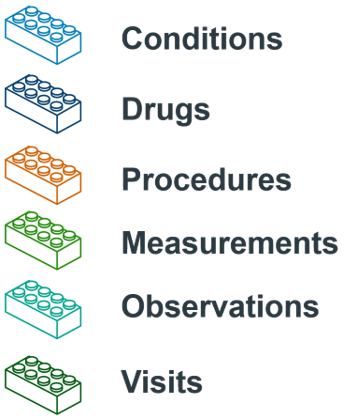
\includegraphics[width=0.5\linewidth]{images/Cohorts/cohort-legos} 

}

\caption{코호트 정의를 위한 빌딩 블록}\label{fig:cohortLegos}
\end{figure}

코호트 정의를 작성할 때, 다음과 같은 질문에 답할 수 있어야 한다:

\begin{itemize}
\tightlist
\item
  \emph{코호트 진입 시간을 정의하는 초기 이벤트는 무엇인가?}
\item
  \emph{초기 이벤트에는 어떤 포함 기준이 적용되는가?}
\item
  \emph{코호트 종료 시간을 정의하는 것은 무엇인가?}
\end{itemize}

\textbf{코호트 진입 이벤트}: 코호트 진입 이벤트(초기 이벤트)는 사람들이
코호트에 진입하는 \textbf{코호트 색인 날짜(cohort index date)} 로
정의된다. 코호트 진입 이벤트는 약물 노출(Drug exposure), 질병
상태(conditions), 절차(procedures), 측정(measurements) 및 방문(visits)과
같은 CDM에 기록된 모든 사건일 수 있다. 초기 이벤트는 데이터가 저장되는
CDM 도메인(예: PROCEDURS\_OCCURRENCE, DRUG\_EXPOSURE 등), 임상 활동을
식별하기 위해 구축된 개념 모음(예 : 질병 상태에 대한 SNOMED 코드, 약물에
대한 RxNorm 코드) 및 기타 특정 속성들(예 : 발생 연령, 첫 진단 / 절차 등,
지정된 시작 및 종료 날짜, 방문 유형 등)에 의해 정의된다. 진입 이벤트를
가진 사람들의 집합을 \textbf{초기 이벤트 코호트} 라고 한다.
\index{cohort!entry event}

\textbf{포함 기준}: 포함 기준은 초기 이벤트 코호트에 적용되어 코호트에
진입할 사람들을 추가적으로 제한한다. 각 포함 기준을 만들 때는 데이터가
저장되는 CDM 도메인, 컨셉 모음, 도메인 별 속성(예 : days supply, 방문
유형) 및 코호트 색인 날짜에 관한 시간 논리를 결정해야 한다. \textbf{적격
코호트(qualifying cohort)} 는 초기 이벤트 코호트에서 모든 포함 기준을
충족하는 사람들의 집합으로 정의한다. \index{cohort!inclusion criteria}

\textbf{코호트 종료 기준}: 코호트 종료 이벤트는 한 사람이 더 이상 코호트
자격 요건을 갖추지 못했을 때를 의미한다. 코호트 종료는 관찰 기간이
끝났을 때, 초기 진입 이벤트로부터 일정한 시간이 경과했을 때 혹은 마지막
이벤트가 발생했을 때 등 여러 방법으로 정의할 수 있다. 코호트 종료 기준에
따라 한 사람이 다른 시간 간격 동안 코호트에 여러 번 속할 수
있다.\index{cohort!exit criteria}

\BeginKnitrBlock{rmdimportant}
OHDSI 도구에는 포함기준과 제외 기준이 구분되지 않는다. 모든 기준은 포함
기준으로 설정해야 한다. 예를 들어 `사전 고혈압 환자 제외'라는 제외
기준을 `사전 고혈압 발생이 0인 사람들 포함'이라는 포함기준으로 설정해야
한다.
\EndKnitrBlock{rmdimportant}

\section{컨셉 모음}\label{conceptSets}

\index{concept set}

컨셉 모음을 구성하는 컨셉들은 다양한 다른 분석들에서 재사용이 가능하다.
컨셉 모음은 관찰 연구들에서 종종 사용되는 표준화된 컴퓨터 코드라고
생각해도 된다. 컨셉 모음은 다음 특성들을 포함하고 있다:

\begin{itemize}
\tightlist
\item
  \textbf{Exclude}: 컨셉 모음으로부터 해당 컨셉과 해당 컨셉의 하위
  컨셉들을 제외하라.
\item
  \textbf{Descendants}: 이 컨셉 뿐만 아니라 모든 하위 항목 컨셉들을
  고려하라.
\item
  \textbf{Mapped}: 표준화되지 않은 컨셉들도 검색하라.
\end{itemize}

예를 들어 표 \ref{tab:conceptSetExpression}과 같이 컨셉 모음은 두 개의
컨셉들을 포함할 수 있다. 여기서 우리는
\href{http://athena.ohdsi.org/search-terms/terms/4329847}{4329847}
(``Myocardial infarction'') 과 그 모든 하위 컨셉들을 포함했고,
\href{http://athena.ohdsi.org/search-terms/terms/314666}{314666} (``Old
myocardial infarction'') 과 그 모든 하위 컨셉들은 제외했다.

\begin{longtable}[]{@{}lllll@{}}
\caption{\label{tab:conceptSetExpression} 컨셉 모음의 예시}\tabularnewline
\toprule
Concept Id & Concept Name & Excluded & Descendants &
Mapped\tabularnewline
\midrule
\endfirsthead
\toprule
Concept Id & Concept Name & Excluded & Descendants &
Mapped\tabularnewline
\midrule
\endhead
4329847 & Myocardial infarction & NO & YES & NO\tabularnewline
314666 & Old myocardial infarction & YES & YES & NO\tabularnewline
\bottomrule
\end{longtable}

그림 \ref{fig:conceptSet}에서 볼 수 있다시피, ``Myocardial infarction''
과 그 모든 하위 컨셉들을 포함할 것이고, 하위 컨셉들 중에서 ``Old
myocardial infarction'' 와 그 모든 하위 컨셉들은 제외할 것이다.
결과적으로 거의 100개 정도의 표준 컨셉들을 포함한 컨셉 모음이
만들어졌다. 이 표준 컨셉들은 다양한 데이터베이스에서 사용되는 수백 개의
소스 코드(예 : ICD-9, ICD-10)를 반영한다.

\begin{figure}

{\centering 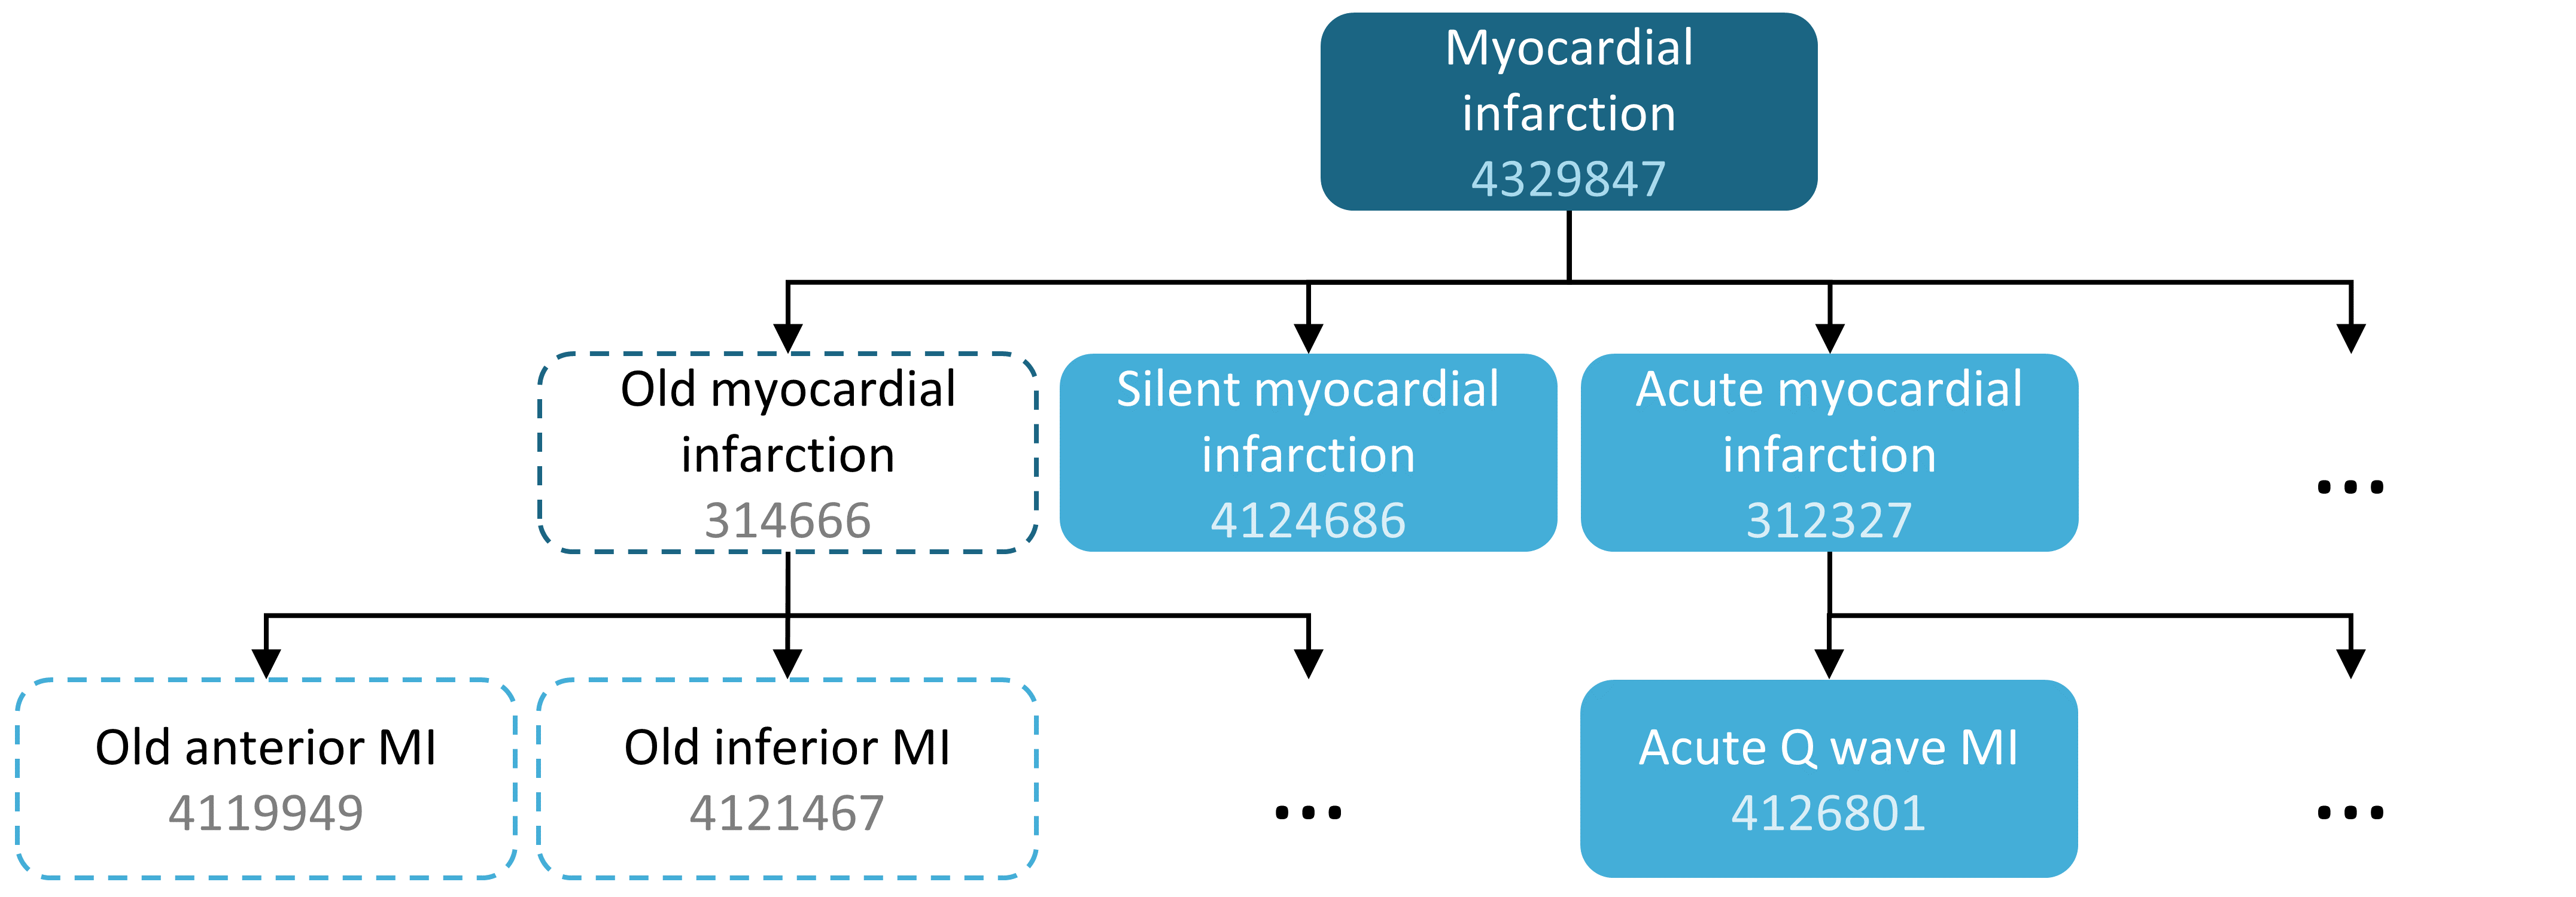
\includegraphics[width=1\linewidth]{images/Cohorts/conceptSet} 

}

\caption{"Myocardial infaction"와 그 하위 컨셉을 포함하지만 "Old myocardial infarction"과 그 하위 컨셉은 제외하는 컨셉 모음}\label{fig:conceptSet}
\end{figure}

\section{확률적 코호트 정의}\label{--}

규칙 기반 코호트 정의는 코호트 정의를 수행할 때 널리 사용되는 방법이다.
그러나 코호트를 만들기 위해 전문가끼리의 합의를 이루는 것은 매우 많은
시간이 소요되는 일이다. 확률적 코호트 정의는 코호트 속성의 효율적인
선택을 위한 대안적인 기계 구동 방식이다. 이 접근법에서, 지도 기계학습은
코호트를 설계하는 알고리즘이 레이블이 붙은 케이스로부터 학습할 수 있게
한다. 이 알고리즘은 더 나은 코호트 설계를 위해 사용될 것이다.
\index{cohort!probabilistic design}

A이 접근 방법을 CDM의 데이터에 적용한 예는 아프로디테 (APHRODITE:
Automated PHenotype Routine for Observational Definition,
Identification, Training and Evaluation) R 패키지이다. 이 패키지는
불완전하게 레이블이 붙은 데이터로부터 학습하는 능력을 결합한 코호트 구축
프레임워크를 제공한다. \citep{Banda2017APHRODITE} \index{APHRODITE}

\section{Cohort Definition Validity}\label{cohort-definition-validity}

당신이 코호트를 구축할 때, 다음 중 당신에게 더 중요한 것이 무엇인지
고려하는 것이 필요하다: \emph{코호트 조건에 해당하는 환자를 모두 찾는
것이 더 중요한가? 아니면 당신이 확신할 수 있는 환자들만 찾는 것이 더
중요한가?}

코호트를 구축할 때 당신의 전략은 전문가가 질병을 얼마나 엄격하게
정의하는지에 의존할 것이다. 얻을 수 있는 모든 것을 사용하거나, 최저 공통
분모를 사용하거나 이 둘을 절충하는 코호트 정의를 작성할 수 있다. 관심
코호트를 적절하게 연구하기 위해 얼마나 엄격한 임계값을 사용할 지는
궁극적으로 연구원의 재량에 달려 있다.

이 장의 시작 부분에서 언급했듯이 코호트 정의는 데이터로부터 관찰하고자
하는 것을 유추하려는 시도이다. 우리는 코호트 정의를 통한 다음의 시도에
성공하였는가? 일반적으로, `골드 스탠다드 기준'과 비교함으로써 규칙
기반의 코호트 정의와 확률적 알고리즘의 유효성을 검증할 수 있다. 이에
대해서는 \ref{ClinicalValidity} 장 (``임상 유효성'')에서 자세히
설명한다.

\subsection{오디시의 골드 스탠다드 코호트 라이브러리}\label{----}

커뮤니티를 지원하기 위해서 OHDSI Gold Standard Phenotype Library (GSPL)
그룹이 형성되었다. GSPL 그룹의 목표는 규칙 기반 및 확률적 방법으로
커뮤니티 기반의 코호트 라이브러리를 개발하는 것이다. GSPL은 OHDSI
커뮤니티의 멤버들이 각자의 연구를 위해 커뮤니티가 검증한 코호트를 찾아서
실행시킬 수 있게 하였다. 이 `gold standard' 코호트들은 라이브러리 안에
들어 있다. GSPL과 관련된 추가적인 정보를 얻으려면 OHDSI 작업 그룹
페이지에 문의하라. 이전에 소개되었던 APHRODITE
\citep{Banda2017APHRODITE} 와 PheValuator tool
\citep{Swerdel2019phevaluator} 뿐만 아니라 OHDSI 네트워크에서 전자 의무
기록과 유전 정보를 공유하기 위해 만들어진 eMERGE Phenotype Library
\href{https://emerge.mc.vanderbilt.edu/}{eMERGE}
\href{https://phekb.org/phenotypes}{Phenotype Library}
\citep{Hripcsak2019eMERGE} 도 해당 작업 그룹에서 다루고 있다. 당신이
코호트를 설계하는 데 관심이 많다면, 이 작업 그룹에 참여해 보아라.
\index{phenotype library}

\section{고혈압 환자 코호트 작성하기}\label{---}

규칙 기반의 접근 방법으로 코호트를 작성해보자. 이번 예제에서는,
\emph{고혈압의 초기 치료를 위해 ACE inhibitors 단일 치료를 시작한
환자들} 을 찾을 것이다.

이 연습을 진행하면서 표준 감소 차트와 비슷한 코호트를 작성하게 될
것이다. 그림 \ref{fig:CohortPractice}은 우리가 어떤 논리로 코호트를
작성할 지 보여준다.

\begin{figure}

{\centering 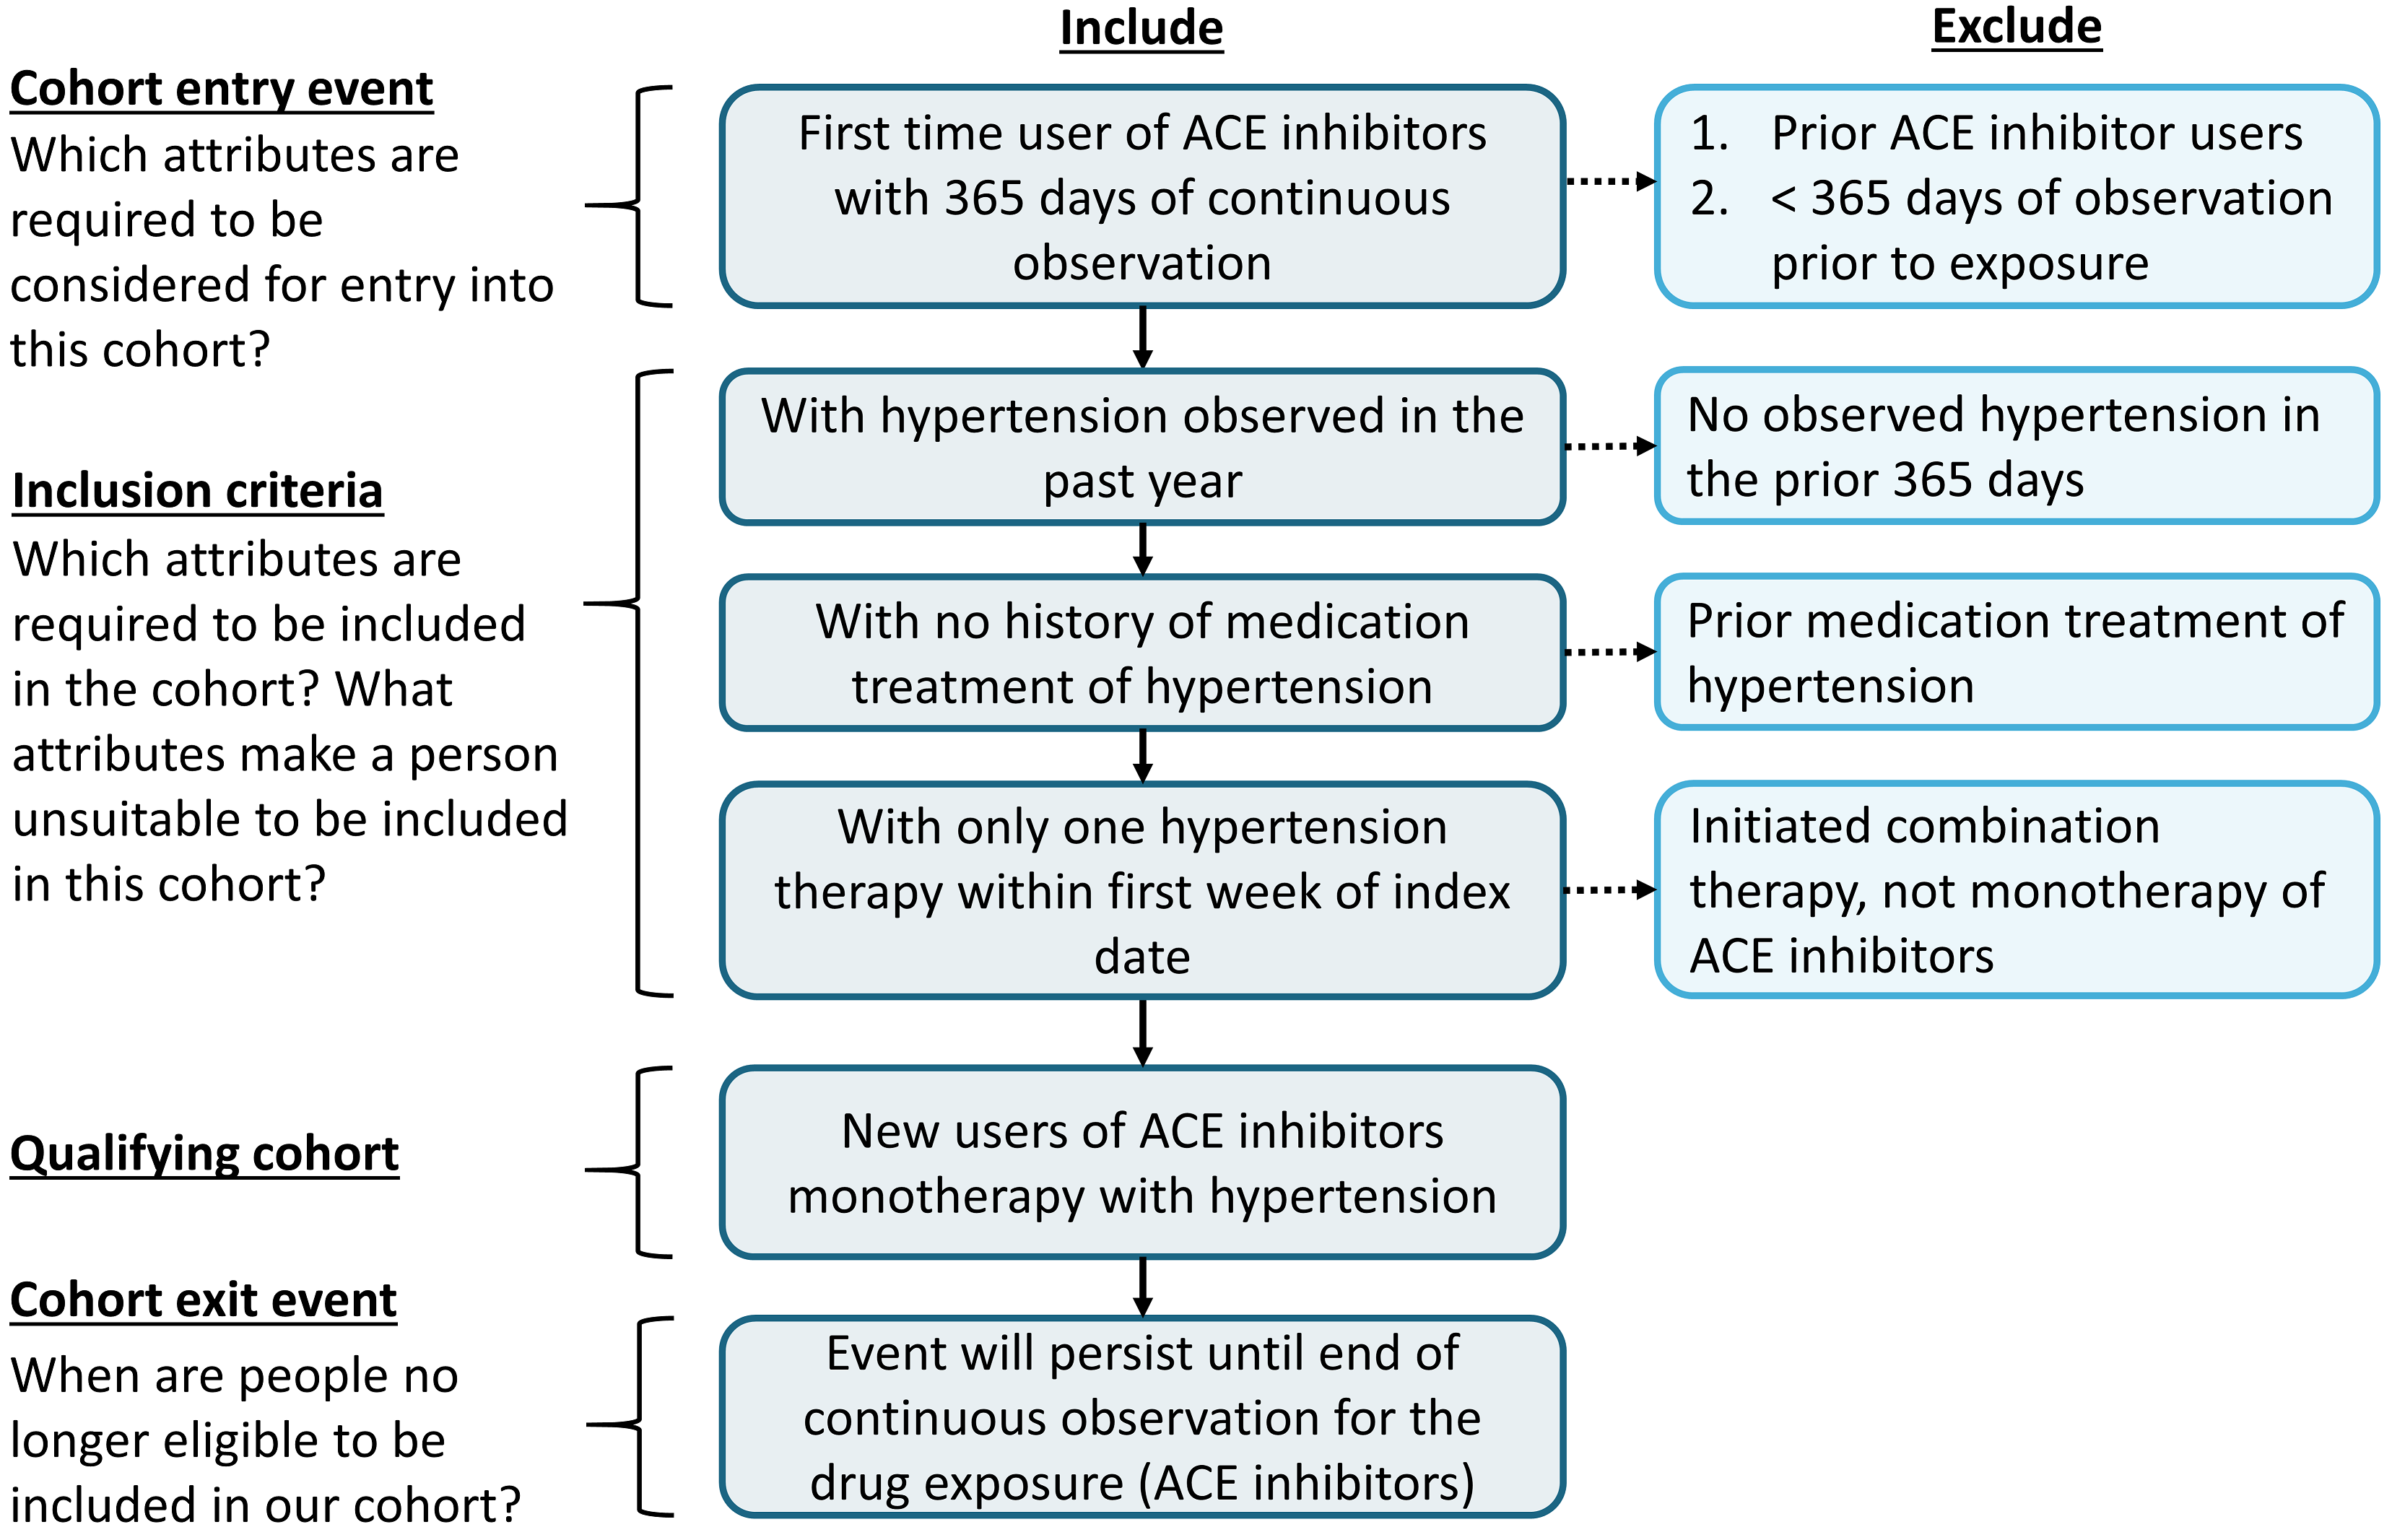
\includegraphics[width=1\linewidth]{images/Cohorts/CohortPractice} 

}

\caption{만들고자 하는 코호트의 논리적 구성도}\label{fig:CohortPractice}
\end{figure}

ATLAS 유저 인터페이스를 사용해서 코호트를 작성해도 되고, 쿼리를 직접
짜도 된다. 이 장에서는 두 가지 방법 모두에 대해 간단히 소개하겠다.

\section{ATLAS를 이용해 코호트 작성하기}\label{atlas---}

ATLAS를 시작하기 위해

\includegraphics{images/Cohorts/cohortdefinition.png} 버튼을 클릭하라.
다음으로 `New cohort' 버튼을 클릭하라. 다음 화면에서 비어 있는 코호트를
확인할 수 있을 것이다. 그림 \ref{fig:ATLASdefineacohort}에서 당신이 현재
보고 있는 화면을 확인하라.

\begin{figure}

{\centering 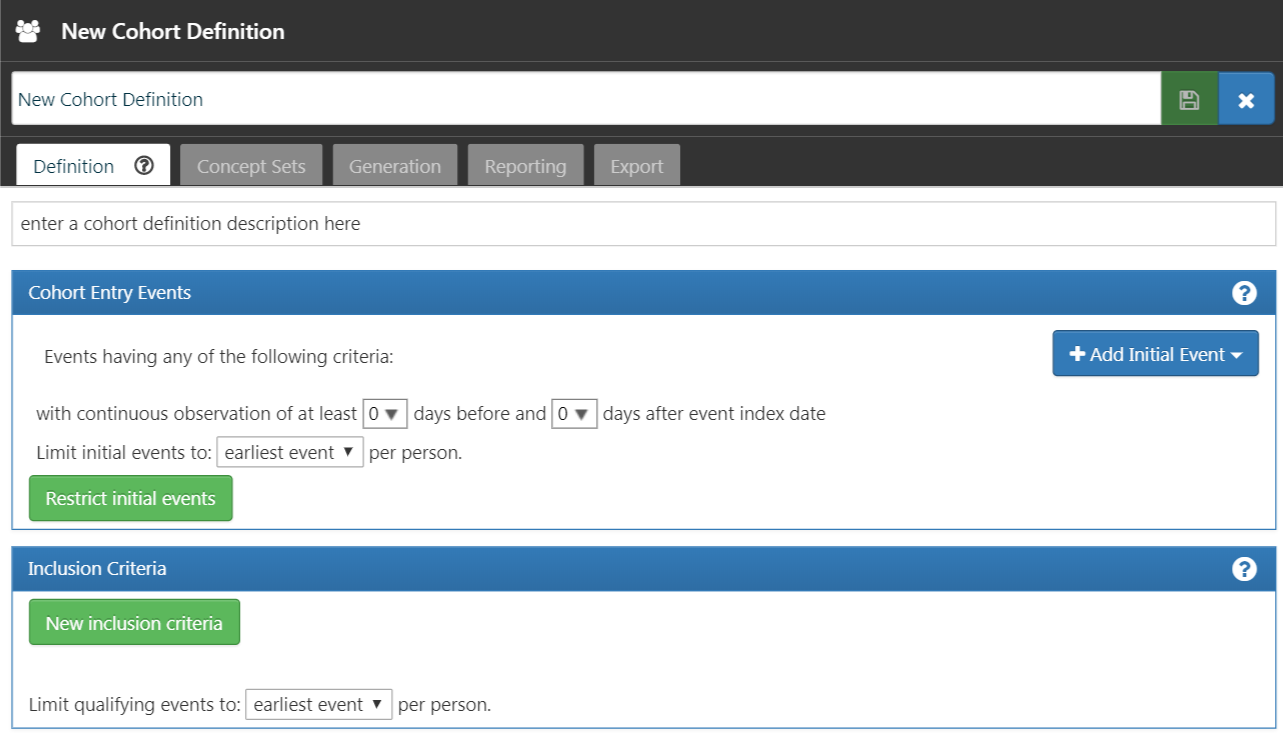
\includegraphics[width=1\linewidth]{images/Cohorts/ATLAS-defineacohort} 

}

\caption{New Cohort Definition}\label{fig:ATLASdefineacohort}
\end{figure}

먼저 ``New Cohort Definition''로 지정되어 있는 코호트 이름을 다른
이름으로 바꾸어 지어주기를 추천한다. `New users of ACE inhibitors as
first-line monotherapy for hypertension' 라고 지으면 적당할 것이다.

\BeginKnitrBlock{rmdimportant}
ATLAS는 동일한 이름을 가진 두 개의 코호트가 존재하는 것을 허락하지
않는다. 기존에 있던 이름을 사용하려고 하면 에러 메시지가 뜰 것이다.
\EndKnitrBlock{rmdimportant}

이름을 정했으면, 
\includegraphics{images/Cohorts/save.png}을 눌러서
코호트를 저장하여라.

\subsection{초기 이벤트 기준}\label{--}

이제 우리는 초기 코호트 이벤트를 정의해야 한다. ``Add initial event''를
클릭하라. 어떤 도메인 내에서 기준을 설정할지 결정해야 한다. 초기 코호트
이벤트를 정의하기 위해 어떤 도메인이 필요한지 어떻게 알 수 있을까? 함께
알아보자.

\begin{figure}

{\centering 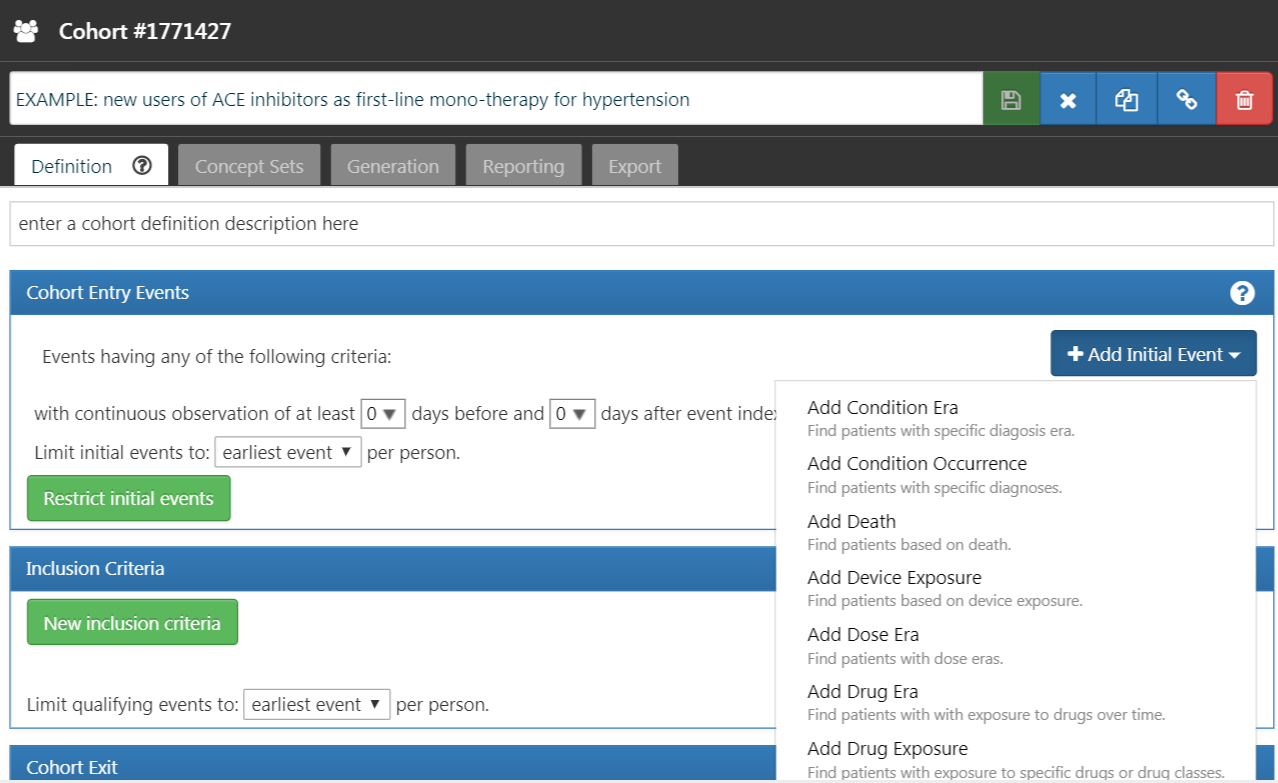
\includegraphics[width=1\linewidth]{images/Cohorts/ATLAS-initialevent} 

}

\caption{초기 이벤트 추가하기}\label{fig:ATLASinitialevent}
\end{figure}

그림 \ref{fig:ATLASinitialevent}에서 볼 수 있듯이 ATLAS는 각 기준들
아래에 설명을 제공한다. 우리가 만약 특정 질병을 진단받은 환자들을 찾으려
한다면 CONDITION\_OCCURRENCE 도메인에서 기준을 만들어야 한다. 특정
약물이나 특정 계열의 약물을 복용한 환자를 찾고 싶다면, DRUG\_EXPOSURE
도메인에서 기준을 만들어야 한다. 우리는 고혈압의 초치료로 ACE inhibitors
단독요법을 시행한 환자들을 찾고 싶기 때문에, DRUG\_EXPOSURE 도메인에서
기준을 만들어야 한다. 그런데 고혈압을 진단받은 환자도 찾아야 하지
않는가? 고혈압과 관련해서는 다른 기준을 만들 것이다. 하지만 고혈압
약물을 복용하기 시작한 날짜가 코호트 시작 날짜로 설정되며, 고혈압 약물을
복용하기 시작한 것이 코호트의 시작 이벤트가 될 것이다. 고혈압의 진단은
\emph{추가적 적격 기준(additional qualifying criteria)} 이라고 부른다.
이에 관해서는 뒤에서 다시 설명하겠다. 이제 `Add Drug Exposure'를
클릭하라.

화면은 당신이 선택한 기준에 따라 업데이트 되겠지만, 아직 끝난 것은
아니다. 그림 \ref{fig:ATLASdrugexposure}에서 볼 수 있다시피 ATLAS는
우리가 어떤 약물을 찾고자 하는 지 아직 모른다. 우리는 ATLAS에게 어떤
컨셉 모음이 ACE inhibitors와 연관이 있는지 알려주어야 한다.

\begin{figure}

{\centering 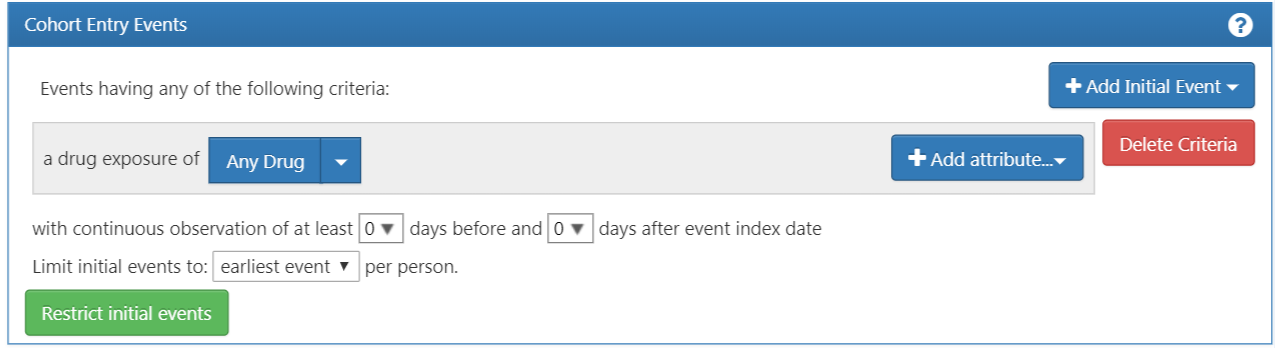
\includegraphics[width=1\linewidth]{images/Cohorts/ATLAS-drugexposure} 

}

\caption{약물 복용에 관하여 정의하기}\label{fig:ATLASdrugexposure}
\end{figure}

\subsection{컨셉 모음 정의하기}\label{--}

ACE inhibitors를 정의하기 위한 대화 상자를 열기 위해
\includegraphics{images/Cohorts/downarrow.png}을 클릭하라.

\subsubsection*{시나리오 1: 당신은 아직 컨셉 모음을 만들지
않았다}\label{-1------}
\addcontentsline{toc}{subsubsection}{시나리오 1: 당신은 아직 컨셉 모음을
만들지 않았다}

아직 당신의 코호트에 추가할 컨셉 모음을 만들지 않았다면, 이것을 먼저
진행해야 한다. `Concept set' 탭의 `New Concept Set'을 클릭하여 코호트를
작성하는 데 쓰일 컨셉 모음을 만들 수 있다. 컨셉 모음의 이름을 `Unnamed
Concept Set'에서 새로 지어 주어야 한다. 이제
\includegraphics{images/Cohorts/search-2.png} 모듈을 통해 ACE
inhibitors를 나타내는 컨셉들을 찾아보자. (그림 \ref{fig:aceinhibitors})

\begin{figure}

{\centering \includegraphics[width=1\linewidth]{images/Cohorts/aceinhibitors} 

}

\caption{용어 찾기 - ACE Inhibitors}\label{fig:aceinhibitors}
\end{figure}

필요한 용어들을 찾았다면,
\includegraphics{images/Cohorts/shoppingcart.png}을 클릭함으로써 그
컨셉을 선택할 수 있다. 그림 \ref{fig:aceinhibitors}의 좌상단의 왼쪽을
향하는 화살표버튼을 클릭하여 코호트 작성 페이지로 돌아갈 수 있다. 적절한
용어를 찾기 위한 방법은 \ref{StandardizedVocabularies}장 (표준 용어)을
참고하라.

그림 \ref{fig:aceConceptSetExpression}에서 우리가 선택한 컨셉 모음의
구성을 확인할 수 있다. 우리는 모든 ACE inhibitors 성분들을 선택했으며,
그것들의 하위 개념들도 포함시켰다. `Included concepts'를 클릭하여 포함된
21,536개의 모든 컨셉들을 확인할 수 있고, `Included Source Codes'를
클릭하여 모든 소스 코드들을 확인할 수도 있다.

\begin{figure}

{\centering \includegraphics[width=1\linewidth]{images/Cohorts/aceConceptSetExpression} 

}

\caption{ACE inhibitor를 포함한 약물들의 컨셉 모음}\label{fig:aceConceptSetExpression}
\end{figure}

\subsubsection*{시나리오 2: 당신은 이미 컨셉 모음을
만들었다}\label{-2-----}
\addcontentsline{toc}{subsubsection}{시나리오 2: 당신은 이미 컨셉 모음을
만들었다}

만약 당신이 이미 컨셉 모음을 만들었고, ATLAS에 저장했다면, `Import
Concept Set'을 클릭하라. 그러면 그림 \ref{fig:ATLASfindyourconcept}에서
볼 수 있다시피 ATLAS의 컨셉 모음 저장소에서 당신의 컨셉 모음을 찾을 수
있는 대화창이 뜬다. 이번 예시에서는 사용자가 ATLAS에 저장되어 있던 컨셉
모음을 이용한다고 가정하자. 사용자는 검색 창에 `ace inhibitors'를
검색하였고, 검색 내용이 이름에 포함된 컨셉 모음들을 볼 수 있을 것이다.
사용자는 해당하는 컨셉 모음을 클릭하여 선택할 수 있다(참고 : 당신이 컨셉
모음을 선택하면 대화창은 사라진다). Any Drug 칸이 당신이 선택한 컨셉
모음의 이름으로 바뀌어 있다면 성공한 것이다.

\begin{figure}

{\centering \includegraphics[width=1\linewidth]{images/Cohorts/ATLAS-findingyourconcept} 

}

\caption{ATLAS 저장소에서 컨셉 모음을 가져오기}\label{fig:ATLASfindyourconcept}
\end{figure}

\subsection{추가적 초기 이벤트 기준}\label{---}

이제 코호트에 컨셉 모음을 만들어 붙였지만, 아직 끝난 것이 아니다. 당신은
ACE inhibitors를 태어나서 처음 복용한 사람들을 찾고 있다. 이는 ACE
inhibitors을 처음 복용한 환자 기록을 찾는 것을 의미한다. 이를 지정하기
위해 당신은 `+Add attribute'를 클릭하여 `Add first exposure criteria'를
선택해야 한다. 당신이 만든 기준의 다른 특성들을 지정할 수 있다는 것을
참고하라. 약물을 복용한 날짜나 나이, 성별 혹은 약물과 관련한 다른
특성들을 지정할 수 있다. 각 도메인에 따라 선택할 수 있는 특성들이
다르다.

선택을 했으면, 창은 자동적으로 닫힌다. 선택된 특성은 초기 기준과 같은 칸
안에서 볼 수 있을 것이다(그림 \ref{fig:initialEventAce}을 보라).

\BeginKnitrBlock{rmdimportant}
현재 ATLAS 디자인은 활용하기에 약간 혼란스러울 수 있다. 생긴 모양과는
다르게 버튼 \includegraphics{images/Cohorts/redX.png}는 `NO'를 의미하는
것이 아니다. 이는 사용자에게 해당 기준을 삭제할 수 있도록 만들어진
버튼이다. 만약 당신이 \includegraphics{images/Cohorts/redX.png}를
클릭한다면, 해당 기준은 사라질 것이다. 그러므로 당신의 기준을 사라지지
않은 채 그대로 보존시키고 싶다면, 옆에
\includegraphics{images/Cohorts/redX.png} 버튼을 그대로 놔 두어야 한다.
\EndKnitrBlock{rmdimportant}

이제 당신은 만족스러운 초기 이벤트를 설정했다. 환자가 처음으로 약물을
복용했다는 사실을 보증하기 위해, 환자 기록을 확인할 수 있는 충분한
기간을 설정해 주면 좋을 것이다. 짧은 관찰 기간을 가진 환자들은 우리가
확인할 수 없는 다른 곳에서 약물을 복용하였을 수도 있다. 우리가 이것을
강제적으로 막을 수는 없지만 index date 이전에 관찰 기간을 설정함으로써
최소한 해당 관찰 기간 동안에는 약물 복용이 이루어지지 않았음을 보증할 수
있다. 이를 위해 관찰 기간을 설정하는 부분이 있으며, 구체적인 관찰 기간을
직접 설정할 수도 있다. 우리는 초기 이벤트 이전에 365일 동안 관찰된
환자를 필요로 한다. 그림 \ref{fig:initialEventAce}처럼 관찰 기간을
다음과 같이 설정하라: \emph{with continuous observation of 365 days
before.} 당신 연구 팀의 재량껏 관찰 기간을 설정하면 된다. 다른
코호트에서는 관찰 기간을 다르게 설정해서 다양한 시도들을 해볼 수 있다.
이는 환자의 과거력에 관한 기간이며, index date 이후의 시간은 포함하지
않는다. 그러므로 우리는 0 dates after index date 라고 설정해야 한다.
우리는 생에 처음 ACE inhibitors를 복용한 환자를 찾고 싶기 때문에
\emph{limit initial events to the ``earliest event'' per person} (한
환자에서 발생한 여러 번의 ACE inhibitor 복용 중, 첫 번째 복용을 초기
이벤트로 설정하는 것)으로 설정한다.

\begin{figure}

{\centering \includegraphics[width=1\linewidth]{images/Cohorts/initialEventAce} 

}

\caption{Index date 이전에 필요로 하는 관찰 기간 설정하기.}\label{fig:initialEventAce}
\end{figure}

지금껏 설정한 논리를 한 눈에 보기 위해서 환자의 타임라인을 설정해볼 수
있다.

\begin{figure}

{\centering \includegraphics[width=1\linewidth]{images/Cohorts/EarliestEventExplained} 

}

\caption{기준들이 적용됨에 따라 환자가 코호트에 적합한지 살펴보기}\label{fig:EarliestEventExplained}
\end{figure}

그림 \ref{fig:EarliestEventExplained}에서 각 행은 코호트에 들어올 자격을
갖출 수 있는 환자 개개인을 나타낸다. 그리고 색칠이 된 별들은 환자가 특정
기준을 만족했던 시간을 나타낸다. 추가적인 기준들이 설정될수록 색칠이 된
별들 대신 그 자리에 색칠되지 않은 별들이 그려진 것을 볼 수 있다. 이는
환자가 조건들을 모두 만족하는 이벤트도 가지고 있지만, 그렇지 않은
이벤트도 가지고 있음을 의미한다. 마지막 기준을 그린 그림을 보면 우리는
ACE inhibitors를 처음으로 복용하였으며, 복용 이전에 최소 365일의 관찰
기간을 가진 환자들을 확인할 수 있다. 당신의 코호트를 설계할 때
\href{http://forums.ohdsi.org}{OHDSI Forum}에 참여하는 연구자들의 의견을
참고하면 더 좋을 것이다.

\subsection{포함 기준}\label{-}

코호트 진입 이벤트를 설정했으면, 다음 두 옵션을 통해 추가적 이벤트를
설정할 수 있다: `Restrict initial events', 그리고 `New inclusion
criteria'. 이 두 옵션 사이에는 ATLAS가 사용자에게 어떤 임시 정보를
제공하는가의 차이가 있다. 만약 당신이 기준을 추가하기 위해 `Restrict
initial events'를 사용한다면, ATLAS에서 카운트를 생성(generate)할 때,
모든 기준들을 충족시키는 사람의 수를 얻게 될 것이다. `New inclusion
criteria'를 통해 기준을 추가한다면, 추가 포함 기준을 적용하여 손실된
환자 수를 보여주는 감소 차트를 확인할 수 있을 것이다. 당신이 추가한
기준에 의해 얼마나 많은 손실이 발생하는지 보여주는 감소 차트를 확인하는
것은 중요하기 때문에 `New inclusion criteria'를 통해 기준을 추가하는
것이 권장된다. 이를 통해 코호트에 포함되는 환자 수를 급격하게 감소시키는
기준이 무엇인지 확인할 수 있게 된다. 당신은 해당 기준을 완화하여 보다 큰
코호트를 얻을 수 있다. 이것은 궁극적으로 이 코호트를 설계하는 전문가의
재량에 달려있다.

이제 `New inclusion criteria'를 통해 기준들을 추가해보자. 이는 위에서
코호트 기준을 설정한 것과 동일한 방법으로 하면 된다. 특정 기준들을
만들어서 넣은 다음, 특정 속성들을 추가할 수 있을 것이다. 우리가 첫
번째로 추가할 기준은 다음과 같다: \emph{ACE inhibitors 약물을 복용한
시점 이후 0\textasciitilde{}365일 이내에 최소 1회 고혈압이 발생한 사람.}
`New inclusion criteria'를 클릭한 다음, 그 기준을 설명해줄 수 있는
이름을 정하라. 그래야 나중에 이 코호트를 다시 보았을 때 자신이 무엇을
만들었는지 헷갈리지 않을 것이다.

이 새로운 기준에 이름을 달고 난 다음, ``+Add criteria to group'' 버튼을
클릭하여 여러 규칙을 담은 기준을 설계하라. 이 버튼은 ``Add Initial
Event''과 비슷한데, 다만 ``+Add criteria to group''의 버튼은 초기
이벤트를 설계하고, 수정하는 버튼이 아니다. 우리는 여기서 여러 개의
기준을 추가할 수 있다. 예를 들어 만약 당신이 질병의 발생을 확인하는
여러가지 방법을 가지고 있다고 가정하자(예: CONDITION\_OCCURRENCE, 혹은
DRUG\_EXPOSURE, 혹은 MEASUREMENT을 사용한 방법). 모두 다른 도메인들이고
각각 다른 기준들을 필요로 하겠지만 특정 조건을 찾는 하나의 기준으로
그룹화할 수 있다. 이 경우에는, 우리는 고혈압의 진단을 찾고 싶기 때문에
``Add condition occurrence''를 선택한다. 여기에 적절한 컨셉 모음을
붙이는 등 초기 이벤트를 설정할 때와 비슷하게 하면 된다. 또한 ACE
inhibitor 첫 복용한 날(index date)로 이후 0\textasciitilde{}365일의
기간을 설정하라. 그림 \ref{fig:ATLASIC1}와 같이 작성될 수 있을 것이다.

\begin{figure}

{\centering \includegraphics[width=1\linewidth]{images/Cohorts/ATLAS-IC1} 

}

\caption{추가적 포함 기준 1}\label{fig:ATLASIC1}
\end{figure}

그리고 당신은 환자들을 탐색할 또다른 기준을 추가하고 싶을 것이다:
\emph{with exactly 0 occurrences of hypertension drugs ALL days before
and 1 day before index start date (ACE inhibitor 이전에 어떠한 고혈압
약물도 복용하지 않은 사람).} 먼저 ``New inclusion criteria''를 클릭해
당신의 기준을 설정한 다음, ``+Add criteria to group''을 클릭한다. 이는
DRUG\_EXPOSURE의 영역이니 ``Add Drug Exposure''를 클릭한 다음, 고혈압
약물의 컨셉 모음을 붙인다. 그리고, index date로부터 ALL days before and
0 days after라는 시간을 설정해준다. exactly 0 occurrence를 선택하였는지
다시 한 번 확인하고 그림 \ref{fig:ATLASIC2}과 같이 잘 만들어졌는지
확인하라.

\begin{figure}

{\centering \includegraphics[width=1\linewidth]{images/Cohorts/ATLAS-IC2} 

}

\caption{추가적 포함 기준 1}\label{fig:ATLASIC2}
\end{figure}

``having no occurrences'' (발생하지 않았다)라는 말이 왜 ``exactly 0
occurrences'' (발생 횟수 0회) 라고 쓰이는 지 혼란스러울 수 있다. 이는
ATLAS 가 사용하는 규칙이다. ATLAS는 오직 포함 기준만을 사용하고, 제외
기준을 사용하지 않는다. 만약 당신이 어떤 특성을 가진 환자들을 제외하고
싶다면 해당 특성을 0회 가지는 환자들을 포함한다는 말로 대체하여야 한다.
처음에는 헷갈릴 수 있지만 계속 사용하다 보면 이러한 논리가 익숙해질
것이다.

마지막으로 목표 환자군 설정을 위한 기준을 하나 더 추가해야 한다:
\emph{with exactly 1 occurrence of hypertension drugs between 0 days
before and 7 days after index start date AND can only start one HT drug
(an ACE inhibitor) -- index date 이후 0\textasciitilde{}7일 동안 정확히
1회의 고혈압 약물을 복용했으며, 반드시 ACE inhibitor로 고혈압 약물치료를
시작해야 한다.} 먼저 ``New inclusion criteria''를 클릭해 당신의 기준을
설정한 다음, ``+Add criteria to group''을 클릭한다. 이는
DRUG\_EXPOSURE의 영역이니 ``Add Drug Exposure''를 클릭한 다음, 고혈압
약물의 컨셉 모음을 붙인다. 그리고 index date 이후
0\textasciitilde{}7일이라는 시간을 설정해준다. 그림 \ref{fig:ATLASIC3}를
통해 진행된 모습을 확인하라.

\begin{figure}

{\centering \includegraphics[width=1\linewidth]{images/Cohorts/ATLAS-IC3} 

}

\caption{추가적 포함 기준 3}\label{fig:ATLASIC3}
\end{figure}

\subsection{코호트 종료 기준}\label{--}

이제 모든 적절한 포함 기준을 추가했다. 다음으로 코호트 종료 기준을
정해야 한다. 사람들이 더 이상 이 코호트에 포함될 자격이 없어질 때는
언제일지 생각해보아야 할 것이다. 이 코호트에서 우리는 약물을 처음 복용한
사람들을 추적한다. 즉, 약물 복용을 중단한 시점에 환자는 코호트에서
나오게 하면 된다. 약물 복용이 중단되는 동안에는 해당 환자에게 무슨 일이
일어나는지 확인할 수 없기 때문이다. 또한 약물 복용 사이에 허용되는
공백기간을 지정하기 위해 persistence 창에서 기준을 설정할 수 있다. 이
연구에서 전문가들은 약물 복용 사이에 최대 30일의 공백기간은 허용된다고
결론지었다.

\textbf{왜 공백기간이 허용되는가?} 우리는 데이터 세트에서 실제로
이루어지는 일들의 일부만 관찰할 수 있을 뿐이다. 특히 환자의 약물 복용에
관한 정보는 처방전의 기록으로 확인한다. 그리고 처방전을 통해 하루 치
이상의 약을 처방하기 때문에 기록이 비어 있는 시간 동안에도 환자가 약을
복용하고 있다는 합리적 추론이 가능하다.

Event will persist ``end of a continuous drug exposure'' 를 선택하고,
persistence 창에 ``allow for a maximum of 30 days''를 추가한 다음 `ACE
inhibitor' 컨셉 모음을 추가로 지정해 주면 된다. 그림
\ref{fig:ATLAScohortexit}를 통해 이를 확인하라.

\begin{figure}

{\centering \includegraphics[width=1\linewidth]{images/Cohorts/cohort-exit} 

}

\caption{코호트 종료 기준}\label{fig:ATLAScohortexit}
\end{figure}

이 코호트의 경우 다른 Censoring event는 선택되지 않았다. 하지만
Censoring event를 추가해야 하는 다른 코호트를 만들어야 할 때, 코호트
정의 할 때 다른 속성들을 추가했던 것과 비슷하게 진행하면 된다. 당신은
이제 당신의 코호트를 성공적으로 만들었다. 반드시
\includegraphics{images/Cohorts/save.png} 버튼을 눌러라. 축하한다!
코호트를 만드는 것은 OHDSI가 제공하는 툴을 이용하기 위해 가장 중요한
부분이다. 이제 `Export' 탭을 클릭하면 ATLAS에 당신이 정의한 코호트가
SQL코드와 JSON 파일로 저장되어 다른 연구자들과 공유할 수 있다.

\section{SQL을 사용하여 코호트 구현하기}\label{sql---}

여기서는 동일한 코호트를 SQL과 R을 통하여 작성하는 방법을 설명할 것이다.
9장에서 설명하였듯이 OHDSI는 SqlRender, DatabaseConnector라는 두 개의 R
패키지를 제공하는데, 이는 SQL의 코드가 다양한 플랫폼에서 실행될 수
있게끔 자동적으로 번역해준다.

구체적인 설명을 위해 우리는 SQL 코드를 여러 개의 단계로 나눌 것이고, 각
단계에서는 다음 단계에 필요한 임시 테이블이 생성될 것이다. 이런 설명
방법이 가장 효율적이지는 않겠지만 매우 긴 단일 명령문을 읽는 것보단 쉬울
것이다.

\subsection{데이터베이스에 연결하기}\label{-}

처음으로 우리는 R에 서버에 어떻게 접속하는 지 알려주어야 한다.
\texttt{createConnectionDetails}라는 기능을 가진
\href{https://ohdsi.github.io/DatabaseConnector/}{DatabaseConnector}
패키지를 사용할 것이다. \texttt{?createConnectionDetails}를 기입하여
다양한 데이터베이스 관리 시스템 (DBMS) 에 연결하기 위해 필요한 설정들을
확인할 수 있다. 예를 들어 아래의 코드를 이용해 PostgreSQL에 연결할 수
있다:

\begin{Shaded}
\begin{Highlighting}[]
\KeywordTok{library}\NormalTok{(CohortMethod)}
\NormalTok{connDetails <-}\StringTok{ }\KeywordTok{createConnectionDetails}\NormalTok{(}\DataTypeTok{dbms =} \StringTok{"postgresql"}\NormalTok{,}
                                       \DataTypeTok{server =} \StringTok{"localhost/ohdsi"}\NormalTok{,}
                                       \DataTypeTok{user =} \StringTok{"joe"}\NormalTok{,}
                                       \DataTypeTok{password =} \StringTok{"supersecret"}\NormalTok{)}

\NormalTok{cdmDbSchema <-}\StringTok{ "my_cdm_data"}
\NormalTok{cohortDbSchema <-}\StringTok{ "scratch"}
\NormalTok{cohortTable <-}\StringTok{ "my_cohorts"}
\end{Highlighting}
\end{Shaded}

마지막 3 줄은 변수 \texttt{cdmDbSchema}, \texttt{cohortDbSchema}, 그리고
\texttt{cohortTable} 들을 정의한다. 우리는 나중에 이 변수들을 R에게 CDM
포멧의 데이터가 어디에 위치해 있으며, 우리가 만든 코호트가 어디에
생성되어야 하는지 알려주기 위해 사용할 것이다. Microsoft SQL
Server에서는 \texttt{cdmDbSchema\ \textless{}-\ "my\_cdm\_data.dbo"}의
예시와 같이 데이터베이스와 스키마 모두를 지정해 주어야 함을 참고하라.

\subsection{컨셉 결정하기}\label{-}

가독성을 위해 R에 필요한 컨셉 아이디들을 정의하고 SQL에 전달한다:

\begin{Shaded}
\begin{Highlighting}[]
\NormalTok{aceI <-}\StringTok{ }\KeywordTok{c}\NormalTok{(}\DecValTok{1308216}\NormalTok{, }\DecValTok{1310756}\NormalTok{, }\DecValTok{1331235}\NormalTok{, }\DecValTok{1334456}\NormalTok{, }\DecValTok{1335471}\NormalTok{, }\DecValTok{1340128}\NormalTok{, }\DecValTok{1341927}\NormalTok{,}
          \DecValTok{1342439}\NormalTok{, }\DecValTok{1363749}\NormalTok{, }\DecValTok{1373225}\NormalTok{)}

\NormalTok{hypertension <-}\StringTok{ }\DecValTok{316866}

\NormalTok{allHtDrugs <-}\StringTok{ }\KeywordTok{c}\NormalTok{(}\DecValTok{904542}\NormalTok{, }\DecValTok{907013}\NormalTok{, }\DecValTok{932745}\NormalTok{, }\DecValTok{942350}\NormalTok{, }\DecValTok{956874}\NormalTok{, }\DecValTok{970250}\NormalTok{, }\DecValTok{974166}\NormalTok{,}
                  \DecValTok{978555}\NormalTok{, }\DecValTok{991382}\NormalTok{, }\DecValTok{1305447}\NormalTok{, }\DecValTok{1307046}\NormalTok{, }\DecValTok{1307863}\NormalTok{, }\DecValTok{1308216}\NormalTok{,}
                  \DecValTok{1308842}\NormalTok{, }\DecValTok{1309068}\NormalTok{, }\DecValTok{1309799}\NormalTok{, }\DecValTok{1310756}\NormalTok{, }\DecValTok{1313200}\NormalTok{, }\DecValTok{1314002}\NormalTok{,}
                  \DecValTok{1314577}\NormalTok{, }\DecValTok{1317640}\NormalTok{, }\DecValTok{1317967}\NormalTok{, }\DecValTok{1318137}\NormalTok{, }\DecValTok{1318853}\NormalTok{, }\DecValTok{1319880}\NormalTok{,}
                  \DecValTok{1319998}\NormalTok{, }\DecValTok{1322081}\NormalTok{, }\DecValTok{1326012}\NormalTok{, }\DecValTok{1327978}\NormalTok{, }\DecValTok{1328165}\NormalTok{, }\DecValTok{1331235}\NormalTok{,}
                  \DecValTok{1332418}\NormalTok{, }\DecValTok{1334456}\NormalTok{, }\DecValTok{1335471}\NormalTok{, }\DecValTok{1338005}\NormalTok{, }\DecValTok{1340128}\NormalTok{, }\DecValTok{1341238}\NormalTok{,}
                  \DecValTok{1341927}\NormalTok{, }\DecValTok{1342439}\NormalTok{, }\DecValTok{1344965}\NormalTok{, }\DecValTok{1345858}\NormalTok{, }\DecValTok{1346686}\NormalTok{, }\DecValTok{1346823}\NormalTok{,}
                  \DecValTok{1347384}\NormalTok{, }\DecValTok{1350489}\NormalTok{, }\DecValTok{1351557}\NormalTok{, }\DecValTok{1353766}\NormalTok{, }\DecValTok{1353776}\NormalTok{, }\DecValTok{1363053}\NormalTok{,}
                  \DecValTok{1363749}\NormalTok{, }\DecValTok{1367500}\NormalTok{, }\DecValTok{1373225}\NormalTok{, }\DecValTok{1373928}\NormalTok{, }\DecValTok{1386957}\NormalTok{, }\DecValTok{1395058}\NormalTok{,}
                  \DecValTok{1398937}\NormalTok{, }\DecValTok{40226742}\NormalTok{, }\DecValTok{40235485}\NormalTok{)}
\end{Highlighting}
\end{Shaded}

\subsection{약물을 처음 복용한 환자 찾기}\label{----}

먼저 각 환자에 대한 ACE inhibitor의 첫 복용을 찾을 것이다:

\begin{Shaded}
\begin{Highlighting}[]
\NormalTok{conn <-}\StringTok{ }\KeywordTok{connect}\NormalTok{(connectionDetails)}

\NormalTok{sql <-}\StringTok{ "SELECT person_id AS subject_id,}
\StringTok{  MIN(drug_exposure_start_date) AS cohort_start_date}
\StringTok{INTO #first_use}
\StringTok{FROM @cdm_db_schema.drug_exposure}
\StringTok{INNER JOIN @cdm_db_schema.concept_ancestor}
\StringTok{  ON descendant_concept_id = drug_concept_id}
\StringTok{WHERE ancestor_concept_id IN (@ace_i)}
\StringTok{GROUP BY person_id;"}

\KeywordTok{renderTranslateExecuteSql}\NormalTok{(conn,}
\NormalTok{                          sql,}
                          \DataTypeTok{cdm_db_schema =}\NormalTok{ cdmDbSchema,}
                          \DataTypeTok{ace_i =}\NormalTok{ aceI)}
\end{Highlighting}
\end{Shaded}

DRUG\_EXPOSURE 테이블을 CONCEPT\_ANCESTOR 테이블에 조인함으로서 ACE
inhibitor를 포함하는 모든 약물을 찾았다는 것을 참고하라.

\subsection{약물 복용 이전 최소 365일동안 관찰될 수 있었던
환자}\label{----365----}

OBSERVATION\_PERIOD 테이블을 조인하여 약물 복용 이전 최소 365일동안
관찰될 수 있었던 환자를 선택해야 한다:

\begin{Shaded}
\begin{Highlighting}[]
\NormalTok{sql <-}\StringTok{ "SELECT subject_id,}
\StringTok{  cohort_start_date}
\StringTok{INTO #has_prior_obs}
\StringTok{FROM #first_use}
\StringTok{INNER JOIN @cdm_db_schema.observation_period}
\StringTok{  ON subject_id = person_id}
\StringTok{    AND observation_period_start_date <= cohort_start_date}
\StringTok{    AND observation_period_end_date >= cohort_start_date}
\StringTok{WHERE DATEADD(DAY, 365, observation_period_start_date) < cohort_start_date;"}

\KeywordTok{renderTranslateExecuteSql}\NormalTok{(conn, sql, }\DataTypeTok{cdm_db_schema =}\NormalTok{ cdmDbSchema)}
\end{Highlighting}
\end{Shaded}

\subsection{이전에 고혈압을 진단받은 환자}\label{---}

index date로부터 365일 이내에 고혈압 진단을 받은 환자여야 한다:

\begin{Shaded}
\begin{Highlighting}[]
\NormalTok{sql <-}\StringTok{ "SELECT DISTINCT subject_id,}
\StringTok{  cohort_start_date}
\StringTok{INTO #has_ht}
\StringTok{FROM #has_prior_obs}
\StringTok{INNER JOIN @cdm_db_schema.condition_occurrence}
\StringTok{  ON subject_id = person_id}
\StringTok{    AND condition_start_date <= cohort_start_date}
\StringTok{    AND condition_start_date >= DATEADD(DAY, -365, cohort_start_date)}
\StringTok{INNER JOIN @cdm_db_schema.concept_ancestor}
\StringTok{  ON descendant_concept_id = condition_concept_id}
\StringTok{WHERE ancestor_concept_id = @hypertension;"}

\KeywordTok{renderTranslateExecuteSql}\NormalTok{(conn,}
\NormalTok{                          sql,}
                          \DataTypeTok{cdm_db_schema =}\NormalTok{ cdmDbSchema,}
                          \DataTypeTok{hypertension =}\NormalTok{ hypertension)}
\end{Highlighting}
\end{Shaded}

\texttt{SELECT\ DISTINCT}를 사용하여 과거에 여러 번의 고혈압 진단을 받은
환자들이 여러 번의 코호트 진입을 하지 않도록 했다.

\subsection{사전에 받은 치료가 없어야 함}\label{----}

이전에 어떠한 고혈압 약물이라도 복용해서는 안 된다:

\begin{Shaded}
\begin{Highlighting}[]
\NormalTok{sql <-}\StringTok{ "SELECT subject_id,}
\StringTok{  cohort_start_date}
\StringTok{INTO #no_prior_ht_drugs}
\StringTok{FROM #has_ht}
\StringTok{LEFT JOIN (}
\StringTok{  SELECT *}
\StringTok{  FROM @cdm_db_schema.drug_exposure}
\StringTok{  INNER JOIN @cdm_db_schema.concept_ancestor}
\StringTok{    ON descendant_concept_id = drug_concept_id}
\StringTok{  WHERE ancestor_concept_id IN (@all_ht_drugs)}
\StringTok{) ht_drugs}
\StringTok{  ON subject_id = person_id}
\StringTok{    AND drug_exposure_start_date < cohort_start_date}
\StringTok{WHERE person_id IS NULL;"}

\KeywordTok{renderTranslateExecuteSql}\NormalTok{(conn,}
\NormalTok{                          sql,}
                          \DataTypeTok{cdm_db_schema =}\NormalTok{ cdmDbSchema,}
                          \DataTypeTok{all_ht_drugs =}\NormalTok{ allHtDrugs)}
\end{Highlighting}
\end{Shaded}

Left join을 사용했으며, DRUG\_EXPOSURE 테이블의 person\_id 행만 NULL의
값(일치하는 기록이 없음을 의미)을 가질 수 있도록 허용했다는 것을
참고하라.

\subsection{단독 요법}\label{-}

코호트에 진입하고 첫 1주일 동안은 고혈압 치료 약물을 단 1회만 복용하도록
설정한다:

\begin{Shaded}
\begin{Highlighting}[]
\NormalTok{sql <-}\StringTok{ "SELECT subject_id,}
\StringTok{  cohort_start_date}
\StringTok{INTO #monotherapy}
\StringTok{FROM #no_prior_ht_drugs}
\StringTok{INNER JOIN @cdm_db_schema.drug_exposure}
\StringTok{  ON subject_id = person_id}
\StringTok{    AND drug_exposure_start_date >= cohort_start_date}
\StringTok{    AND drug_exposure_start_date <= DATEADD(DAY, 7, cohort_start_date)}
\StringTok{INNER JOIN @cdm_db_schema.concept_ancestor}
\StringTok{  ON descendant_concept_id = drug_concept_id}
\StringTok{WHERE ancestor_concept_id IN (@all_ht_drugs)}
\StringTok{GROUP BY subject_id,}
\StringTok{  cohort_start_date}
\StringTok{HAVING COUNT(*) = 1;"}

\KeywordTok{renderTranslateExecuteSql}\NormalTok{(conn,}
\NormalTok{                          sql,}
                          \DataTypeTok{cdm_db_schema =}\NormalTok{ cdmDbSchema,}
                          \DataTypeTok{all_ht_drugs =}\NormalTok{ allHtDrugs)}
\end{Highlighting}
\end{Shaded}

\subsection{코호트 종료}\label{-}

이제 코호트 종료 일자를 제외하고 코호트를 완전히 지정했다. 코호트는
노출이 중단되면 종료되도록 정의되며, 노출 사이에 최대 30일의 간격까지는
허용된다. 즉, 약물의 복용 시작 뿐만 아니라 ACE inhibitor의 후속 복용에
대해서도 고려한다는 말이다. SQL을 통해 약물의 후속 복용을 고려하여 약물
복용 기간을 정의하는 것은 매우 복잡하다. 운이 좋게도 약물 복용 기간을
효율적으로 만들 수 있는 표준 코드가 작성되었다. 이 코드는 Chris Knoll이
작성했으며 OHDSI 내에서 종종 마법이라고 불리는 코드이기도 하다. 먼저
병합하려는 모든 약물 복용을 포함하는 임시 테이블을 만든다:

\begin{Shaded}
\begin{Highlighting}[]
\NormalTok{sql <-}\StringTok{ "}
\StringTok{  SELECT person_id,}
\StringTok{    CAST(1 AS INT) AS concept_id,}
\StringTok{    drug_exposure_start_date AS exposure_start_date,}
\StringTok{    drug_exposure_end_date AS exposure_end_date}
\StringTok{  INTO #exposure}
\StringTok{  FROM @cdm_db_schema.drug_exposure}
\StringTok{  INNER JOIN @cdm_db_schema.concept_ancestor}
\StringTok{    ON descendant_concept_id = drug_concept_id}
\StringTok{  WHERE ancestor_concept_id IN (@ace_i);"}
\KeywordTok{renderTranslateExecuteSql}\NormalTok{(conn,}
\NormalTok{                          sql,}
                          \DataTypeTok{cdm_db_schema =}\NormalTok{ cdmDbSchema,}
                          \DataTypeTok{ace_i =}\NormalTok{ aceI)}
\end{Highlighting}
\end{Shaded}

그런 다음 순차적 복용을 병합하기 위한 표준 코드를 실행한다:

\begin{Shaded}
\begin{Highlighting}[]
\NormalTok{sql <-}\StringTok{ "}
\StringTok{SELECT ends.person_id AS subject_id,}
\StringTok{    ends.concept_id AS cohort_definition_id,}
\StringTok{  MIN(exposure_start_date) AS cohort_start_date,}
\StringTok{  ends.era_end_date AS cohort_end_date}
\StringTok{INTO #exposure_era}
\StringTok{FROM (}
\StringTok{  SELECT exposure.person_id,}
\StringTok{    exposure.concept_id,}
\StringTok{    exposure.exposure_start_date,}
\StringTok{    MIN(events.end_date) AS era_end_date}
\StringTok{  FROM #exposure exposure}
\StringTok{  JOIN (}
\StringTok{--cteEndDates}
\StringTok{    SELECT person_id,}
\StringTok{      concept_id,}
\StringTok{      DATEADD(DAY, - 1 * @max_gap, event_date) AS end_date}
\StringTok{    FROM (}
\StringTok{      SELECT person_id,}
\StringTok{        concept_id,}
\StringTok{        event_date,}
\StringTok{        event_type,}
\StringTok{        MAX(start_ordinal) OVER (}
\StringTok{          PARTITION BY person_id ,concept_id ORDER BY event_date,}
\StringTok{              event_type ROWS UNBOUNDED PRECEDING}
\StringTok{          ) AS start_ordinal,}
\StringTok{        ROW_NUMBER() OVER (}
\StringTok{          PARTITION BY person_id, concept_id ORDER BY event_date,}
\StringTok{            event_type}
\StringTok{          ) AS overall_ord}
\StringTok{      FROM (}
\StringTok{-- select the start dates, assigning a row number to each}
\StringTok{        SELECT person_id,}
\StringTok{          concept_id,}
\StringTok{          exposure_start_date AS event_date,}
\StringTok{          0 AS event_type,}
\StringTok{          ROW_NUMBER() OVER (}
\StringTok{            PARTITION BY person_id, concept_id ORDER BY exposure_start_date}
\StringTok{            ) AS start_ordinal}
\StringTok{        FROM #exposure exposure}

\StringTok{        UNION ALL}
\StringTok{-- add the end dates with NULL as the row number, padding the end dates by}
\StringTok{-- @max_gap to allow a grace period for overlapping ranges.}

\StringTok{        SELECT person_id,}
\StringTok{          concept_id,}
\StringTok{          DATEADD(day, @max_gap, exposure_end_date),}
\StringTok{          1 AS event_type,}
\StringTok{          NULL}
\StringTok{        FROM #exposure exposure}
\StringTok{        ) rawdata}
\StringTok{    ) events}
\StringTok{  WHERE 2 * events.start_ordinal - events.overall_ord = 0}
\StringTok{  ) events}
\StringTok{  ON exposure.person_id = events.person_id}
\StringTok{      AND exposure.concept_id = events.concept_id}
\StringTok{      AND events.end_date >= exposure.exposure_end_date}
\StringTok{  GROUP BY exposure.person_id,}
\StringTok{      exposure.concept_id,}
\StringTok{      exposure.exposure_start_date}
\StringTok{  ) ends}
\StringTok{GROUP BY ends.person_id,}
\StringTok{  concept_id,}
\StringTok{  ends.era_end_date;"}

\KeywordTok{renderTranslateExecuteSql}\NormalTok{(conn,}
\NormalTok{                          sql,}
                          \DataTypeTok{cdm_db_schema =}\NormalTok{ cdmDbSchema,}
                          \DataTypeTok{max_gap =} \DecValTok{30}\NormalTok{)}
\end{Highlighting}
\end{Shaded}

이 코드는 모든 후속 복용들을 병합하며, \texttt{max\_gap}의 변수를 통해
약물 복용 사이에 허용되는 최대기간을 정의할 수 있다. 그 결과로 작성된
약물 복용 기간은 임시 테이블 \texttt{\#exposure\_era}라고 불리는 임시
테이블에 기록된다. 다음으로 ACE inhibitor 복용 기간을 우리의 기존
코호트에 조인하기만 하면, ACE inhibitor 복용 종료 날짜를 우리의 코호트
종료 날짜로써 사용할 수 있게 된다.

\begin{Shaded}
\begin{Highlighting}[]
\NormalTok{sql <-}\StringTok{ "SELECT ee.subject_id,}
\StringTok{  CAST(1 AS INT) AS cohort_definition_id,}
\StringTok{  ee.cohort_start_date,}
\StringTok{  ee.cohort_end_date}
\StringTok{INTO @cohort_db_schema.@cohort_table}
\StringTok{FROM #monotherapy mt}
\StringTok{INNER JOIN #exposure_era ee}
\StringTok{  ON mt.subject_id = ee.subject_id}
\StringTok{    AND mt.cohort_start_date = ee.cohort_start_date;"}

\KeywordTok{renderTranslateExecuteSql}\NormalTok{(conn,}
\NormalTok{                          sql,}
                          \DataTypeTok{cohort_db_schema =}\NormalTok{ cohortDbSchema,}
                          \DataTypeTok{cohort_table =}\NormalTok{ cohortTable)}
\end{Highlighting}
\end{Shaded}

이제 우리가 정의한 최종 코호트를 스키마와 테이블에 저장해야 한다. 우리는
코호트 정의 ID를 1로 설정하여 동일한 테이블에 저장된 다른 코호트들과
구별할 것이다.

\subsection{정리하기}

마지막으로, 작성된 임시 테이블을 정리하고 데이터베이스 서버와의 연결을
끊는 것이 좋다:

\begin{Shaded}
\begin{Highlighting}[]
\NormalTok{sql <-}\StringTok{ "TRUNCATE TABLE #first_use;}
\StringTok{DROP TABLE #first_use;}

\StringTok{TRUNCATE TABLE #has_prior_obs;}
\StringTok{DROP TABLE #has_prior_obs;}

\StringTok{TRUNCATE TABLE #has_ht;}
\StringTok{DROP TABLE #has_ht;}

\StringTok{TRUNCATE TABLE #no_prior_ht_drugs;}
\StringTok{DROP TABLE #no_prior_ht_drugs;}

\StringTok{TRUNCATE TABLE #monotherapy;}
\StringTok{DROP TABLE #monotherapy;}

\StringTok{TRUNCATE TABLE #exposure;}
\StringTok{DROP TABLE #exposure;}

\StringTok{TRUNCATE TABLE #exposure_era;}
\StringTok{DROP TABLE #exposure_era;"}

\KeywordTok{renderTranslateExecuteSql}\NormalTok{(conn, sql)}

\KeywordTok{disconnect}\NormalTok{(conn)}
\end{Highlighting}
\end{Shaded}

\section{요약}\label{-4}

\BeginKnitrBlock{rmdsummary}
\begin{itemize}
\item
  코호트는 일정 기간 동안 하나 이상의 포함 기준을 만족시키는 사람들의
  집합이다.
\item
  코호트 정의는 특정 코호트를 식별하는 데 사용되는 논리에 대한 설명이다.
\item
  코호트는 OHDSI 분석 도구 전체에서 사용(및 재사용)될 수 있다.
\item
  코호트를 작성하기 위한 두 가지 주요 접근 방법이 있다: 규칙 기반 정의,
  확률적 정의
\item
  규칙 기반의 코호트 정의는 ATLAS나 SQL을 통해 작성될 수 있다.
\end{itemize}
\EndKnitrBlock{rmdsummary}

\section{실습}

\subsubsection*{전제 조건}\label{--2}
\addcontentsline{toc}{subsubsection}{전제 조건}

첫 번째 실습으로, ATLAS에 접근이 필요하다.
\url{http://atlas-demo.ohdsi.org}를 통해 접속하거나, 다른 접속방법을
이용해도 된다.

\BeginKnitrBlock{exercise}
\protect\hypertarget{exr:exerciseCohortsAtlas}{}{\label{exr:exerciseCohortsAtlas}
}ATLAS를 이용하여 아래의 기준에 따라 코호트를 작성하라:

\begin{itemize}
\tightlist
\item
  diclofenac을 복용하기 시작한 환자들
\item
  16세 이상의 환자들
\item
  약물 복용 이전 최소 365일 간 관찰이 되어 있던 환자들
\item
  이전에 NSAID (Non-Steroidal Anti-Inflammatory Drug) 를 복용하지 않은
  환자들
\item
  이전에 암을 진단받지 않은 환자들
\item
  약물 복용 중단을 코호트 종료로 정의 (30일 이하의 약물 미복용 기간은
  허용)
\end{itemize}
\EndKnitrBlock{exercise}

\subsubsection*{전제 조건}\label{--3}
\addcontentsline{toc}{subsubsection}{전제 조건}

두 번째 실습을 수행하기 위해서 \ref{installR}절에서 설명된 것처럼 R과
R-Studio, 그리고 자바가 설치되어 있다고 가정한다. 또한 아래의 코드를
사용하여 \href{https://ohdsi.github.io/SqlRender/}{SqlRender},
\href{https://ohdsi.github.io/DatabaseConnector/}{DatabaseConnector},
그리고 \href{https://ohdsi.github.io/Eunomia/}{Eunomia} 패키지를
설치하라:

\begin{Shaded}
\begin{Highlighting}[]
\KeywordTok{install.packages}\NormalTok{(}\KeywordTok{c}\NormalTok{(}\StringTok{"SqlRender"}\NormalTok{, }\StringTok{"DatabaseConnector"}\NormalTok{, }\StringTok{"devtools"}\NormalTok{))}
\NormalTok{devtools}\OperatorTok{::}\KeywordTok{install_github}\NormalTok{(}\StringTok{"ohdsi/Eunomia"}\NormalTok{, }\DataTypeTok{ref =} \StringTok{"v1.0.0"}\NormalTok{)}
\end{Highlighting}
\end{Shaded}

Eunomia 패키지는 당신의 로컬 R 세션에서 수행될 CDM의 데이터를 제공한다.
아래의 코드를 이용하여 연결할 수 있다.

\begin{Shaded}
\begin{Highlighting}[]
\NormalTok{connectionDetails <-}\StringTok{ }\NormalTok{Eunomia}\OperatorTok{::}\KeywordTok{getEunomiaConnectionDetails}\NormalTok{()}
\end{Highlighting}
\end{Shaded}

CDM 데이터베이스 스키마는 `main' 이다.

\BeginKnitrBlock{exercise}
\protect\hypertarget{exr:exerciseCohortsSql}{}{\label{exr:exerciseCohortsSql}
}다음 기준에 따르도록 현재 존재하는 코호트 테이블 안에서 급성
심근경색(Acute Myocardial Infarction) 코호트를 SQL과 R을 이용하여 만들어
보자:

\begin{itemize}
\tightlist
\item
  심근 경색을 진단받은 사람들 (컨셉 4329847 'Myocardial infarction'과
  이것의 그 하위 컨셉들에서 컨셉 314666 'Old myocardial infarction'과 그
  모든 하위 컨셉들을 제외하기)
\item
  입원환자 혹은 응급실 방문 환자만 선택 (컨셉 9201'Inpatient Visit',
  9203 `Emergency Room Visit'), 262 `Emergency Room and Inpatient
  Visit')
\end{itemize}
\EndKnitrBlock{exercise}

해답은 부록 \ref{Cohortsanswers}에 있다.

\chapter{환자 특성 분석 Characterization}\label{Characterization}

\emph{작성자 : Anthony Sena \& Daniel Prieto-Alhambra}

관찰형 보건의료데이터는 다양한 특성을 바탕으로 인구집단의 변화를 이해할
수 있는 귀중한 자원이다. 기술통계를 통해 인구집단의 특성을 확인하는 것은
건강과 질병에 영향을 주는 요인에 대한 가설 설정을 위한 중요한 첫번째
단계이다. 이번 장에서는 특성 분석 (characterization)을 위한 방법들에
대해 살펴보기로 한다. :

\begin{itemize}
\tightlist
\item
  \textbf{데이터베이스 수준의 특성 분석 (Database-level
  characterization)}: 상위 수준 (top-level)의 요약 통계량을 제공하여
  데이터베이스 전체에 대한 이해를 돕는다.
\item
  \textbf{코호트의 특성 분석 (Cohort characterization)}: 통합된 의무기록
  측면에서 인구집단을 기술한다.
\item
  \textbf{치료 경로 (Treatment pathways)}: 특정 기간동안 한 사람에
  대하여 행해진 중재 (intervention) 순서를 기술한다.
\item
  \textbf{발생 (Incidence)}: 위험 관찰 기간(time at risk, TAR)동안의
  outcome의 발생율을 계산한다.
\end{itemize}

데이터베이스 수준의 특성 분석을 제외하고 이 방법들은 index date라고 하는
시점과 관련된 인구 집단에 대해 설명하는데 목적이 있다. 이와 같은 관심
집단은 코호트라고 정의되며 \ref{Cohorts} 장에 기술되어 있다. 코호트는
관심집단의 개개인에 대한 index date를 정의한다. Index date를 기준으로
index date이전의 시간을 \textbf{기저 시간(baseline time)}이라 정의한다.
Index date를 포함한 그 이후의 시간들은 \textbf{index 후 시간(post-index
time)}이라고 부른다.

특성 분석은 질병의 자연 경과, 치료 이용, 진료 질 개선 등과 같은 것에
활용될 수 있다. 이번 장에서는 특성 분석 방법에 대해 기술하며, ATLAS와
R을 이용한 고혈압 환자군에 대한 특성 분석을 해 볼
것이다.\index{characterization}
\index{cohort characterization|see {characterization!cohort}}
\index{baseline time} \index{post-index time} \index{index date}
\index{disease natural history|see {characterization}}
\index{treatment utilization|see {characterization}}
\index{quality improvement|see {characterization}}

\section{데이터베이스 수준의 특성 분석 (Database Level
Characterization)}\label{----database-level-characterization}

관심집단에 대한 특성 분석을 시행하기 전, 사용하고자 하는 데이터베이스의
특성을 이해하는 것이 선행되어야 한다. 데이터베이스 수준의 특성 분석은
전체 데이터베이스에 대한 시간의 흐름에 따른 경향과 분포 측면에서 데이터
번체를 설명하기 위해 사용한다. 데이터베이스의 정량적 분석은 일반적으로
다음과 같은 질문을 포함한다:

\begin{itemize}
\tightlist
\item
  이 데이터베이스의 총 사람 수는 몇인가?
\item
  환자들의 연령 분포는 어떠한가?
\item
  환자들의 관찰 기간은 얼마나 오래되었는가?
\item
  시간이 지남에 따라 기록/처방된 \{치료, 질병, 처치 등\}을 받은 사람의
  비율은 어떠한가?
\end{itemize}

데이터베이스 수준의 기술 통계는 연구자로 하여금 어떠한 데이터에서 손실이
있을 수 있는지와 같이 확인할 수 없는 부분을 이해하는데 도움을 주며
\ref{DataQuality} 장 데이터 품질을 설명할 때 자세히 다룬다.
\index{characterization!database level}

\section{코호트 특성 분석 (Cohort
Characterization)}\label{---cohort-characterization}

코호트 특성 분석은 기저 시점과 index 후 코호트 구성원의 특징들을
기술한다. OHDSI는 상태(condition), 약물(drug), 치료재료(device),
시술(procedure), 임상적 관찰(clinical observation) 등 개인의 의무기록에
존재하는 모든 것에 대한 기술 통계량을 바탕으로 특성 분석을 접근한다.
또한, index 시점에서 코호트 구성원에 대한 사회인구학적 내용에 대해
요약해준다. 이와 같은 접근 방식을 통해 관심 코호트에 대한 완벽한 요약을
제공한다. 특히, 이러한 접근을 통해 데이터의 변화에 대한 안목을 가지고
코호트에 대한 전체적인 탐색을 가능하게 하는 한편, 잠재적인 결측 값을
찾을 수 있도록 한다.

코호트 특성 분석 방법은 이미 치료를 받은 사람에서 치료의 적응증 유발율과
금기를 추정하는 개인 수준의 개인 수준의 약물 사용 연구 (person-level
drug utilization studies : DUS)에 이용될 수 있다. 코호트 특성 분석의
보급은 역학 관찰연구 보고 강화(Strengthening the Reporting of
Observational Studies in Epidemiology, STROBE) 가이드라인에 자세히
제시된 관찰 연구에 권장되는 모범사례이다. \citep{VONELM2008344}
\index{characterization!cohort}
\index{descriptive statistics|see {characterization}}
\index{drug utilization}

\section{치료 경로 (Treatment Pathways)}\label{--treatment-pathways}

인구 집단의 특성을 분석하는 또 하나의 방법은 index 후(post-index) 시간
동안의 치료 순서를 기술하는 것이다. 예를들어, 이전
연구\citep{Hripcsak7329}에서 OHDSI의 공통 데이터 표준을 활용해 제 2형
당뇨, 고혈압, 우울증에 대한 치료 경로의 특징을 분석하기 위한 기술 통계를
고안하였다. 이러한 분석 방법을 표준화 함으로써, Hripcsak과 그 연구팀은
관심집단의 특성 분석을 OHDSI 네트워크 상에서 동일한 통계방법으로
실행하였다. \index{characterization!treatment pathways}
\index{treatment pathways|see {characterization!treatment pathways}}
\index{cohort pathways|see {characterization!treatment pathways}}

치료 경로 분석은 가장 처음 처방/조제된 약물 이후 특정 상태에 있는 환자에
대한 치료행위(events)를 요약하기 위해 시행한다. 이 연구에서는 제 2형
당뇨, 고혈압, 우울증의 진단 이후의 치료행위들을 기술했다. 개개인이 받은
치료행위들(events)은 이후 요약 통계량으로 합쳐지고 각의 질병과 각각의
데이터베이스에서 별로 시각화되었다.

\begin{figure}

{\centering \includegraphics[width=1\linewidth]{images/Characterization/pnasTreatmentPathwaysSunburst} 

}

\caption{고혈압 환자의 OHDSI 치료 경로 "sunburst" 시각화 사례}\label{fig:treatmentPathwaysSunburstDataViz}
\end{figure}

figure \ref{fig:treatmentPathwaysSunburstDataViz}에서 제시된 사례는
고혈압 치료를 시작한 환자집단을 나타낸다. 가운데 위치한 첫번쨰 고리는
1차 요법(first-line therapy)에 대한 환자의 비율을 나타낸다. 이 사례의
경우 Hydrochlorothiazide는 고혈압 환자군의 1차 요법으로 가장 흔하게
사용되는 약물이라는 것을 알 수 있다. Hydrochlorothiazide에서 파생된
상자들은 해당 코호트 대상자에서 기록된 두번째(2nd), 세번째(3rd) 요법을
의미한다.

치료 경로 분석은 인구집단 내의 치료 이용 현황에 대한 중요한 근거를
제공한다. 이 분석을 통해 우리는 가장 빈번히 사용되는 1차 요법을 기술할
수 있고, 치료가 중단/변경/확대된 사람들의 비율을 알 수 있다. 경로 분석을
통해 metformin이 당뇨에서 가장 일반적으로 처방된 1차 치료제임을 밝혔고,
이를 통해 미국 내분비학회의 당뇨 치료 알고리즘의 일차 요법이 일반적으로
잘 적용되고 있음을 확인했다. 더불어 당뇨 환자의 10\%, 고혈압 환자의
24\%, 그리고 우울증 환자의 11\%는 다른 데이터베이스와 비교했을 때 공유된
적 없는 치료 경로를 따르고 있는 것을 확인했다.

고전적인 약물 사용 연구 (DUS) 개념에서, 치료 경로 분석은 특정 집단에서
하나 이상의 약물 사용율과 같은 집단 수준의 약물 사용 연구
(population-level DUS) 뿐 아니라 치료 방법의 지속률, 서로 다른 치료 간의
전환률과 같은 개인 수준의 약물 사용 연구 (person-level DUS)가 포함된다.

\section{발생 (Incidence)}\label{-incidence}

발생률과 발생비는 공중 보건에서 위험 관찰 기간(time-at-risk, TAR)동안
인구집단 내 새로운 outcome의 발생의 평가에 사용되는 통계적 지표이다.
Figure \ref{fig:incidenceTimeline} 는 한 사람에게서 발생률 계산에 필요한
구성요소를 보여주고 있다: \index{incidence}

\begin{figure}

{\centering \includegraphics[width=1\linewidth]{images/Characterization/incidenceTimeline} 

}

\caption{개인 수준에서의 발생률 계산의 구성 성분. 본 예시에서는 위험 관찰 기간은 코호트가 시작하고 하루 이후부터 코호트가 끝나는 시점으로 정의됨.}\label{fig:incidenceTimeline}
\end{figure}

figure \ref{fig:incidenceTimeline}에서 한 사람은 데이터 내에서 관찰이
시작되고 끝나는 시점이 표시된 기간을 갖는다. 그 다음, 그 사람은 몇몇
연구 기준 (eligibility criteria)에 의해 코호트에 들어가는(enter) 시점과
나오는(exit) 시점을 갖게 된다. 위험을 관찰하는 기간(time at risk, TAR)은
우리가 outcome의 발생을 보고자 하는 기간을 의미한다. 만일 outcome이 위험
관찰 기간(time at risk, TAR) 내에서 발생한다면, outcome이 발생된 것으로
간주한다.

발생을 계산하기 위해서는 두 가지 측정법이 있다:

\[ 
발생\;분율 = \frac{\#\;코호트에\;포함된\;사람\;중\;TAR\;동안\;새로운\;outcome이\;있는\;경우}{\#\;TAR을\;가지면서\;코호트에\;포함된\;사람}
\]

발생 분율은 위험 관찰 기간동안 집단 내 새로운 outcome의 발생을 측정하는
방법이다. 다시 말해, 관심집단에서 정해진 시간의 틀 안에서 발생한
outcome의 비율이다. \index{incidence!proportion}

\[
발생률 = \frac{\#\;코호트에\;포함된\;사람\;중\;TAR\;동안\;새로운\;outcome이\;있는\;경우}{코호트에\;포함된\;사람들의\;위험\;노출\;기간\;(TAR)로\;구한\;인-시\;(person\;time\;at\;risk)}
\]

\[
Incidence\;Rate = \frac{\#\;persons\;in\;cohort\;with\;new\;outcome\;during\;TAR}{person\;time\;at\;risk\;contributed\;by\;persons\;in\;cohort}
\]

발생률은 인구집단에서 누적되는 위험 관찰 기간 동안의 새로 발생한
outcome의 횟수를 측정한 것이다. 만일 한 환자가 위험 관찰 기간 (TAR)
내에서 outcome을 경험했을 때, 그 환자가 전체의 인-시(person-time)에
outcome이 발생하기까지의 시간만큼 기여했다고 산정한다. 누적된 위험 관찰
기간은 \textbf{인-시(person-time)}라고 하고, 단위는 일, 월, 혹은 연으로
표현된다. \index{incidence!rate} \index{person-time}

치료 요법에 대하여 계산할 때, 정해진 치료 요법의 사용 비율 혹은 발생률을
계산하는 것은 전형적인 인구 집단 수준의 약물 사용 연구(population-level
DUS)라 할 수 있다.

\section{고혈압 환자의 특성 분석 (Characterizing Hypertensive
Persons)}\label{----characterizing-hypertensive-persons}

세계보건기구(WHO)의 고혈압에 대한 보고서\citep{WHOHypertension}에
따르면, 고혈압의 초기 발견과 적절한 치료 및 양호한 혈압 조절은 건강과
경제적인 면에서 상당한 이득이 있다. WHO의 보고서에는 고혈압의 개요 및
여러 국가들의 질병 부담의 특징들을 보여주고 있다. WHO는 지경과 사회
경제적 계급 및 성별 별 고혈압에 대한 기술통계를 제공하고 있다.

WHO가 수행한 고혈압 환자의 특성 분석과 동일한 분석은 관찰형 데이터
소스를 이용해 할 수 있다. 이 장의 다음 절에서는 고혈압 환자 집단의
구성을 이해하기 위한 데이터베이스의 탐색을 ATLAS와 R을 이용해 시행하는
방법을 살펴볼 것이다. 또한, 동일한 툴을 사용해 고혈압 집단의 자연 경과와
치료 패턴을 알아 설명하려고 한다.

\section{ATLAS를 활용한 데이터베이스의 특성 분석 (Database
Characterization in
ATLAS)}\label{atlas-----database-characterization-in-atlas}

여기서는 ATLAS에 탑재된 데이터 소스 모듈을 사용하여
\href{https://github.com/OHDSI/Achilles}{ACHILLES}로 생성된
데이터베이스의 특성을 살펴보고, 고혈압 환자와 관련된 데이터베이스 수준의
특성을 찾아내는 방법을 설명하고자 한다. 시작하기 위해 ATLAS의 왼쪽 바에
위치한
\includegraphics{images/Characterization/atlasDataSourcesMenuItem.png}을
클릭하자. ATLAS의 첫번째 드롭 다운 목록에서 데이터 탐색(database to
explore)을 선택한다. 그리고, 데이터베이스 아래의 드롭 다운 목록을 통해
보고서를 탐색을 시작할 수 있다. 고혈압 환자에 대한 데이터베이스 수준의
특성 분석을 위해 두 번째 드롭 다운 목록인 report 드롭 다운 목록에서
Condition Occurrence를 선택하면 해당 데이터베이스의 모든 질병에 대한
treemap 시각화 결과가 표시된다:

\begin{figure}

{\centering \includegraphics[width=1\linewidth]{images/Characterization/atlasDataSourcesConditionTreemap} 

}

\caption{Atlas Data Sources: Condition Occurrence Treemap}\label{fig:atlasDataSourcesConditionTreemap}
\end{figure}

특정 관심 질환을 검색하기 위해 Table탭을 클릭하면 환자 수, 유병률, 환자
별 기록들을 포함하는 데이터베이스의 전체 condition 목록이 나타난다.
상단의 filter 상자를 이용해 ``hypertension''을 포함하는 concept name만을
걸러낼 수 있다:

\begin{figure}

{\centering \includegraphics[width=1\linewidth]{images/Characterization/atlasDataSourcesConditionFiltered} 

}

\caption{Atlas Data Sources: concept name에서 "hypertension"이라는 단어를 이용해 걸러낸 결과}\label{fig:atlasDataSourcesConditionFiltered}
\end{figure}

하나의 행을 클릭하면 해당 condition에 대한 자세한 드릴다운 보고서를
확인할 수 있다. 이 경우 ``essential hypertension''을 선택한 결과이며,
선택된 condition의 시간에 따른 경향과 성별, 월별 유병률, 기록 유형
(주상병 혹은 부상병 등) 그리고 최초 진단 시 나이의 경향을 알 수 있다:

\begin{figure}

{\centering \includegraphics[width=1\linewidth]{images/Characterization/atlasDataSourcesDrillDownReport} 

}

\caption{Atlas Data Sources: Essential hypertension drill down report}\label{fig:atlasDataSourcesDrillDownReport}
\end{figure}

지금까지 고혈압이라는 concept에 대한 데이터의 특징과 시간에 따른 경향을
살펴보았다. 데이터베이스 수준의 특성 분석을 통해 고혈압 환자의 치료에
사용된 약물에 대하여도 확인할 수 있다. 이는 RxNorm Ingredient에 요약된
약물의 특성을 검토를 위해 Drug Era report을 사용한 것 외에는 위와
동일하게 진행된다. 관심있는 항목에 대한 데이터베이스 특성 탐색을
마쳤다면, 이제는 특성화 하고자 하는 고혈압 환자의 특성 분석을 위한
코호트를 설계하는 단계로 나아갈 준비를 마친 것이다.

\section{ATLAS를 이용한 코호트 특성 분석 (Cohort Characterization in
ATLAS)}\label{atlas-----cohort-characterization-in-atlas}

이 장에서는 ATLAS를 이용한 대규모의 코호트 특성 분석 방법에 대해 설명할
것이다. ATLAS의 왼쪽 바에 있는
\includegraphics{images/Characterization/atlasCharacterizationMenuItem.png}를
클릭하면, 새로운 특성 분석을 만들 수 있다. 분석을 명명하고
\includegraphics{images/PopulationLevelEstimation/save.png} 버튼을 눌러
저장한다.

\subsection{디자인 (Design)}\label{-design}

특성 분석은 하나 이상의 코호트와 분석하고자 하는 하나 이상의 속성이
필요하다. 예시의 경우, 두 개의 코호트를 사용할 것이다. 첫번째 코호트는
고혈압 치료를 시작한 환자로 index date 이전 1년 간 한번이라도 고혈압
진단을 받은 환자로 정의한다고 하자. 또한 이 코호트에 속한 사람들은
고혈압 치료제를 복용하기 시작한 후 최소 1년의 관찰 기간을 갖는다고 하자
(Appendix \ref{HTN1yrFO}). 두번째 코호트는 첫 번째 코호트와 모든 조건이
동일하지만 최소 관찰기간을 1년 대신 3년을 갖는다고 하자 (Appendix
\ref{HTN3yrFO}).

\subsubsection*{코호트 정의 (Cohort
Definitions)}\label{--cohort-definitions}
\addcontentsline{toc}{subsubsection}{코호트 정의 (Cohort Definitions)}

\begin{figure}

{\centering \includegraphics[width=1\linewidth]{images/Characterization/atlasCharacterizationCohortSelection} 

}

\caption{Characterization design tab - cohort definition selection}\label{fig:atlasCharacterizationCohortSelection}
\end{figure}

해당 코호트들은 \ref{Cohorts} 장에서 이미 만들어 져 있다고 가정한다.
\includegraphics{images/Characterization/atlasImportButton.png}을
클릭하고 figure \ref{fig:atlasCharacterizationCohortSelection}에서
보이는 바와 같이 코호트를 선택한다. 그 다음, 두 코호트 특성 분석을 위해
사용할 속성을 설정한다.

\subsubsection*{속성 선택 (Feature
Selection)}\label{--feature-selection}
\addcontentsline{toc}{subsubsection}{속성 선택 (Feature Selection)}

ATLAS는 OMOP CDM에서 모델링 된 임상 도메인에서 특성 분석을 수행하기 위한
속성들이 100개 이상 사전에 정의되어 있다. 각 사전에 정의된 분석은 선택된
분석 대상 코호트들에 대한 임상 관찰들을 집계하고 요약하는 기능을
수행한다. 이와 같은 계산은 코호트의 기저 그리고 index 후 특징들을
설명하기 위해 수천 가지의 속성을 제공한다. ATLAS는 OHDSI에서 제공하는
FeatureExtraction R package를 이용해 개별 코호트에 대한 특성 분석을
시행하며, 이 FeatureExtraction이라는 R package을 사용하는 방법에 대하여
다음 절에서 더 자세하게 다룰 것이다. \index{feature analyses}

분석하고자 하는 속성들을 선택하기 위해
\includegraphics{images/Characterization/atlasImportButton.png} 를
클릭한다. 아래에는 코호트의 특성 분석을 위해 사용할 속성들의 리스트가
있다:

\begin{figure}

{\centering \includegraphics[width=1\linewidth]{images/Characterization/atlasCharacterizationFeatureSelection} 

}

\caption{Characterization design tab - feature selection.}\label{fig:atlasCharacterizationFeatureSelection}
\end{figure}

위 그림은 각의 코호트에서 분석할 속성들에 어떤 것들이 있는지를 설명과
함께 목록을 나타낸 것이다. ``Demographics''라고 시작하는 속성은 각
환자의 인구 통계학적인 정보를 코호트의 시작 시점에서 계산한다. 도메인
이름으로 시작한 속성들 (예를 들어, Visit, Procedure, Condition, Drug
등)은 해당 도메인에 기록된 모든 관찰 값들의 특성을 나타낸 것이다. 각각의
도메인의 특성들은 코호트 시작 지점에 앞서 네 가지의 시간대의 옵션이
있다:

\begin{itemize}
\item
  \textbf{Any time prior}: 환자의 관찰 기간 내에서 코호트 시작 지점
  이전의 모든 시간대를 사용
\item
  \textbf{Long term}: 코호트 시작 지점을 포함하여 365일 이전까지
\item
  \textbf{Medium term}: 코호트 시작 지점을 포함하여 180일 이전까지
\item
  \textbf{short term}: 코호트 시작 지점을 포함하여 30일 이전까지
\end{itemize}

\subsubsection*{하위 집단 분석 (Subgroup
Analysis)}\label{---subgroup-analysis}
\addcontentsline{toc}{subsubsection}{하위 집단 분석 (Subgroup Analysis)}

만일 성별에 따라 특성에 차이가 있는지가 알고싶다면 어떻게 해야할까? 이때
우리는 ``하위 집단 분석 (subgroup analyses)''을 이용할 수 있다. 이는
특성 분석 안에서 새로운 관심 하위 집단에 대한 정의를 할 수 있도록
해준다. 하위 집단을 만들기 위해 하위 그룹에 대한 기준 (criteria)을
클릭해 더하면 된다. 이 단계는 코호트 정의에 사용되는 기준 (criteria)과
유사하다. 이 사례에서 우리는 코호트 내의 여성을 확인할 수 있는 기준
(criteria) 셋를 정의할 것이다:

\begin{figure}

{\centering \includegraphics[width=1\linewidth]{images/Characterization/atlasCharacterizationSubgroup} 

}

\caption{여성에 대한 하위 그룹 분석을 위한 특성 분석 디자인.}\label{fig:atlasCharacterizationSubgroup}
\end{figure}

\BeginKnitrBlock{rmdimportant}
ATLAS의 하위 그룹 분석은 층화(strata)와 같지 않다. 층화(strata)는
상호배제하는 반면, 하위그룹은 선택된 기준(criteria)에 따라 동일한 사람이
하위그룹에 포함될 수 있다.
\EndKnitrBlock{rmdimportant}

\subsection{실행 (Executions)}\label{-executions}

특성 분석의 설계가 끝났다면, 우리의 환경 내에서 사용할 수 있는 하나
이상의 데이터베이스에 대하여 설계한 특성 분석을 시행할 수 있다.
Execution 탭으로 이동하여 Generate 버튼을 클릭하면 선택된
데이터베이스에서 분석이 시작된다:

\begin{figure}

{\centering \includegraphics[width=1\linewidth]{images/Characterization/atlasCharacterizationExecutions} 

}

\caption{설계한 특성 분석의 실행 - CDM source 선택.}\label{fig:atlasCharacterizationExecutions}
\end{figure}

분석이 완료되면, ``All Executions'' 버튼을 클릭하고 실행 목록에서 ``View
Reports''를 선택하면 보고서를 볼 수 있다. 이와 별도로 ``view latest
result''를 클릭하면 가장 최근에 시행된 분석의 결과를 확인할 수 있다.

\subsection{결과 (Results)}\label{-results}

\begin{figure}

{\centering \includegraphics[width=1\linewidth]{images/Characterization/atlasCharacterizationResultsSummary} 

}

\caption{특성 분석 결과 - condition occurrence long term.}\label{fig:atlasCharacterizationResultsSummary}
\end{figure}

설계 시 선택된 각 코호트의 다른 속성들은 표의 형식으로 나타난다. 그림
\ref{fig:atlasCharacterizationResultsSummary}에서 보이는 것 처럼 코호트
시작 일로부터 365일 이전에 두 코호트에 존재하는 모든 질환을 요약하여
확인할 수 있다. 각 변수들은 개별 코호트와 우리가 코호트 내에서 정의한
여성 하위그룹에 대한 수 (count)와 백분율 (percentage)를 갖는다.

어떤 심혈관 질환들이 모집단에서 관찰되는지 이해하고자
\texttt{cardiac\ arrhythmia} 과거력을 갖는 환자의 비율이 얼마인지를
알아보기 위해 겁색창에서 필터를 사용하였다. cardiac arrythmia concept
옆의 \texttt{Explore} 링크를 이용하면 그림
\ref{fig:atlasCharacterizationResultsExplore}에 보여지는 것과 같이
하나의 코호트에 대하여 더 자세한 내용이 들어있는 새로운 창을 띄울 수
있다:

\begin{figure}

{\centering \includegraphics[width=1\linewidth]{images/Characterization/atlasCharacterizationResultsExplore} 

}

\caption{특성 분석 결과 - 하나의 concept에 대하여 자세한 내용이 들어있는 새로운 창.}\label{fig:atlasCharacterizationResultsExplore}
\end{figure}

분석하고자 하는 코호트들에 대하여 모든 conition에 대한 컨셉을 분석하고
나면, 탐색 옵션을 통해 선택된 모든 컨셉의 모든 상, 하위 관계에 있는
컨셉을 확인할 수 있다. 본 연구의 경우 cardiac arrythmia에 대하여
확인했다. 이와 같은 탐색 기능은 컨셉의 계층 구조를 탐색 할 수 있도록
하며, 고혈압 환자들에서 나타날 수 있는 다른 심장 질환들을 확인할 수
있도록 한다. 요약된 결과처럼 (갯)수와 백분율로써 화면에 출력된다.

동일한 특성 분석은 혈관 부종과 같은 항 고혈압 제제의 부작용에 의한
상태를 찾는 분석에도 사용할 수 있다. 방법은 위의 분석과 동일하게 그림
\ref{fig:atlasCharacterizationResultsContra}에 나온 것 처럼 'edema'를
검색하여 진행할 수 있다:

\begin{figure}

{\centering \includegraphics[width=1\linewidth]{images/Characterization/atlasCharacterizationResultsContra} 

}

\caption{특성 분석 결과 - 금기되는 상태 이상을 탐색한 결과.}\label{fig:atlasCharacterizationResultsContra}
\end{figure}

다시 한 번, 고혈압 환자에서 혈관 부종의 발병률을 알아보기 위해 Edema의
특성을 보는 탐색 기능을 사용할 것이다:

\begin{figure}

{\centering \includegraphics[width=1\linewidth]{images/Characterization/atlasCharacterizationResultsContraExplore} 

}

\caption{특성 분석 결과 - 금기되는 상태 이상에 대한 자세한 결과.}\label{fig:atlasCharacterizationResultsContraExplore}
\end{figure}

항 고혈압 제제를 시작하기 1년 전부터 혈관 부종의 기록이 있었던 사람들의
비율을 확인하 수 있었다.

\begin{figure}

{\centering \includegraphics[width=1\linewidth]{images/Characterization/atlasCharacterizationResultsContinuous} 

}

\caption{각 코호트와 하위 집단의 연령 관련 특성 분석 결과.}\label{fig:atlasCharacterizationResultsContinuous}
\end{figure}

도메인 변수는 이분법적인 표지자를 사용해 계산되는 반면 (즉, 이전
시간대에 존재했던 코드의 기록), 코호트 시작 시점의 연력과 같은 일부
변수들은 연속적인 값을 갖는다. 위의 예시와 같이 두 코호트에서 연령에
대한 특성 분석 결과는 사람의 총 수, 연령의 평균, 연령의 중앙값 그리고
표준 편차를 통해 확인할 수 있었다.

\subsection{사용자 정의 속성 (Defining Custom
Features)}\label{---defining-custom-features}

사전에 정의되어 제공되는 속성들 뿐 아니라 ATLAS에서는 사용자가 필요에
따라 속성들을 커스터마이즈 하고 정의할 수 있는 기능을 지원한다. 왼쪽
메뉴에서 \textbf{characterization}를 클릭하고, \textbf{Feature
Analysis}탭을 클릭 한 후, \textbf{New Feature Analysis} 버튼을 클릭하면
사용자가 정의한 속성 분석을 할 수 있다. 사용자가 정의하는 속성을
명명하고, \includegraphics{images/PopulationLevelEstimation/save.png}
버튼을 통해 저장할 수 있다. \index{ATLAS!characterization features}

예를 들어, 코호트 시작 이후에 ACE inhibitors의 drug era를 갖는 각각의
코호트에 속하는 사람 수를 알아본다고 하자:

\begin{figure}

{\centering \includegraphics[width=1\linewidth]{images/Characterization/atlasCharacterizationCustomFeature} 

}

\caption{ATLAS를 이용한 사용자가 정의하는 속성.}\label{fig:atlasCharacterizationCustomFeature}
\end{figure}

위에서 정의한 기준(criteria)은 코호트 시작 날짜에 적용된다고 가정하자.
이전에 정의한 기준(criteria)을 저장했다면, 이전 절에서 우리가 디자인한
특성 분석에 이를 적용할 수 있다. 이는 위해 characterization을 열고,
Feature Analysis로 이동 해 보자.
\includegraphics{images/Characterization/atlasImportButton.png} 버튼을
누르고 메뉴에서 new custom features를 선택하자. 그러면 분석할 속성
목록에 사용자 정의 속성이 올라간 것이 보일 것이다. 앞 절에서 설명한 것과
같이 사용자 정의 속성에 대한 분석을 데이터베이스에 적용하여 시행할 수
있다:

\begin{figure}

{\centering \includegraphics[width=1\linewidth]{images/Characterization/atlasCharacterizationCustomFeatureResults} 

}

\caption{사용자 정의 속성을 적용하여 특성 분석을 진행한 결과 창}\label{fig:atlasCharacterizationCustomFeatureResults}
\end{figure}

\section{R을 이용한 코호트 특성 분석 (Cohort Characterization in
R)}\label{r-----cohort-characterization-in-r}

코호트의 특성 분석은 R을 통해서도 가능하다. R에서 고혈압 코호트에서 기저
속성(변수)을 생성하기 위해 OHDSI의 FeatureExtraction이라고 하는 R
package를 사용하는 방법을 알아보기로 한다. FeatureExtraction은 세 가지
방법으로 변수를 구성할 수 있는 기능을 제공한다. 그 방법은 다음과 같다:
\index{FeatureExtraction}

\begin{itemize}
\tightlist
\item
  기본 설정된 변수 셋을 선택
\item
  사전 지정된 분석 셋 중에서 선택
\item
  사용자 정의 분석 셋을 생성
\end{itemize}

FeatureExtraction은 개인 수준 속성 (person-level feature)과 통합된
속성의 두가지 방법으로 변수를 만든다. 개인 수준의 특성은 기계 학습에
적용할 때 유용하다. 이 절에서는 관심 코호트를 설명하는 기저 변수를
생성할 때 유용한 통합된 속성의 사용 방법을 집중적으로 설명할 것이다.
더불어 사전 지정된 분석과 사용자가 정의하는 분석의 두 가지 변수를 구성
방법에 대해 알아볼 것이다. (기본 설정 세트에 대해서는 독자의 연습을 위해
남겨두도록 하겠다.)

\subsection{Cohort Instantiation}\label{cohort-instantiation}

특성 분석을 위해 우선 코호트를 예시를 들어 설명하겠다. 코호트 예시는
\ref{Cohorts} 장에서 실습 했었다. 본 실습에서는 고혈압의 1차 약물 치료를
시작한 사람들 중 1년 간 관찰된 사람들을 사용할 것이다 (Appendix
\ref{HTN1yrFO}). 부록 \ref{CohortDefinitions} 의 다른 코호트들은 독자의
연습을 위해 남겨두었다. cohort definition ID가 1인
\texttt{scratch.my\_cohorts} 라는 테이블에 실습에 사용할 코호트가 있다고
가정하자.

\subsection{데이터 추출 (Data Extraction)}\label{--data-extraction}

먼저 R이 서버에 접속할 수 있도록 해야한다. FeatureExtraction은
DatabaseConnector package의 \texttt{createConnectionDetails} 함수를
이용해 서버와 연결할 수 있다. \texttt{?createConnectionDetails}를
입력하면 다양한 데이터베이스 관리 시스템 (DBMS)이 요구하는 설정 값이
어떤것 들이 있는지 확인할 수 있다. 예를 들어, PostgreSql 데이터베이스와
연결해야 하는 경우 다음과 같이 연결 설정을 해야 한다:

\begin{Shaded}
\begin{Highlighting}[]
\KeywordTok{library}\NormalTok{(FeatureExtraction)}
\NormalTok{connDetails <-}\StringTok{ }\KeywordTok{createConnectionDetails}\NormalTok{(}\DataTypeTok{dbms =} \StringTok{"postgresql"}\NormalTok{,}
                                       \DataTypeTok{server =} \StringTok{"localhost/ohdsi"}\NormalTok{,}
                                       \DataTypeTok{user =} \StringTok{"joe"}\NormalTok{,}
                                       \DataTypeTok{password =} \StringTok{"supersecret"}\NormalTok{)}

\NormalTok{cdmDbSchema <-}\StringTok{ "my_cdm_data"}
\NormalTok{cohortsDbSchema <-}\StringTok{ "scratch"}
\NormalTok{cohortsDbTable <-}\StringTok{ "my_cohorts"}
\NormalTok{cdmVersion <-}\StringTok{ "5"}
\end{Highlighting}
\end{Shaded}

마지막 네 줄의 코드는 \texttt{cdmDbSchema}, \texttt{cohortsDbSchema},
\texttt{cohortsDbTable} 변수들을 정의하고 CDM 버전 또한 정의하기
위함이다. 이러한 정의는 나중에 R에게 CDM 형식의 데이터가의 위치, 관심
코호트가 만들어진 위치, 어떤 버전의 CDM이 사용되었는지를 확인할 수
있도록 해준다. Microsofe SQL Server에서 주의할 점은, 데이터베이스
스키마는 데이터베이스와 스키마 정보를 둘 다 필요로 한다는 것이다. 예를
들면 다음과 같다.
\texttt{cdmDbSchema\ \textless{}-\ "my\_cdm\_data.dbo"}.

\subsection{사전 지정 분석의 사용 (Using Prespecified
Analyses)}\label{----using-prespecified-analyses}

\texttt{createCovariateSettings} 함수는 사전에 미리 정의된 대규모
변수들의 셋을 선택할 수 있도록 한다. \texttt{?createCovariateSettings}를
입력하면 사용 가능한 옵션들을 확인할 수 있다. 예를 들어:

\begin{Shaded}
\begin{Highlighting}[]
\NormalTok{settings <-}\StringTok{ }\KeywordTok{createCovariateSettings}\NormalTok{(}
  \DataTypeTok{useDemographicsGender =} \OtherTok{TRUE}\NormalTok{, }
  \DataTypeTok{useDemographicsAgeGroup =} \OtherTok{TRUE}\NormalTok{, }
  \DataTypeTok{useConditionOccurrenceAnyTimePrior =} \OtherTok{TRUE}\NormalTok{) }
\end{Highlighting}
\end{Shaded}

다음과 같이 입력하면 성별, 연령 (5년 단위의 연령 그룹), 그리고 코호트
시작 날짜를 포함한 이전의 모든 condition\_occurrence 테이블에서 관찰된
각각의 컨셉들에 대하여 이분법적인 변수를 생성할 수 있다.

많은 사전 정의 분석은 단기(short term), 중기(medium term), 혹은
장기(long term) 구간(time window)을 지정할 수 있다. 기본적으로 구간들은
다음과 같이 정의 되어 있다:

\begin{itemize}
\tightlist
\item
  \textbf{Long term}: 코호트 시작 날짜를 포함한 365일 이전까지의 구간.
\item
  \textbf{Medium term}: 코호트 시작 날짜를 포함한 180일 이전까지의 구간.
\item
  \textbf{short term}: 코호트 시작 날짜를 포함한 30일 이전까지의 구간.
\end{itemize}

그러나 아래의 예시와 같이 사용자가 시간 구간을 변경 할 수 있다:

\begin{Shaded}
\begin{Highlighting}[]
\NormalTok{settings <-}\StringTok{ }\KeywordTok{createCovariateSettings}\NormalTok{(}\DataTypeTok{useConditionEraLongTerm =} \OtherTok{TRUE}\NormalTok{, }
                                    \DataTypeTok{useConditionEraShortTerm =} \OtherTok{TRUE}\NormalTok{, }
                                    \DataTypeTok{useDrugEraLongTerm =} \OtherTok{TRUE}\NormalTok{,}
                                    \DataTypeTok{useDrugEraShortTerm =} \OtherTok{TRUE}\NormalTok{, }
                                    \DataTypeTok{longTermStartDays =} \OperatorTok{-}\DecValTok{180}\NormalTok{, }
                                    \DataTypeTok{shortTermStartDays =} \OperatorTok{-}\DecValTok{14}\NormalTok{, }
                                    \DataTypeTok{endDays =} \OperatorTok{-}\DecValTok{1}\NormalTok{) }
\end{Highlighting}
\end{Shaded}

이 코드에서 새로 정의된 long-term 구간은 코호트 시작 날짜를 포함하지
않고 180일 이전까지의 구간을 나타내고, short-term 구간은 코호트 시작
날짜를 포함하지 않고 14일 이전까지의 구간을 나타낸다. 또한, 변수
구성에서 필수적으로 들어가야 할 것과 빠져야 할 concept ID를 지정할 수
있다:

\begin{Shaded}
\begin{Highlighting}[]
\NormalTok{settings <-}\StringTok{ }\KeywordTok{createCovariateSettings}\NormalTok{(}\DataTypeTok{useConditionEraLongTerm =} \OtherTok{TRUE}\NormalTok{, }
                                    \DataTypeTok{useConditionEraShortTerm =} \OtherTok{TRUE}\NormalTok{, }
                                    \DataTypeTok{useDrugEraLongTerm =} \OtherTok{TRUE}\NormalTok{, }
                                    \DataTypeTok{useDrugEraShortTerm =} \OtherTok{TRUE}\NormalTok{, }
                                    \DataTypeTok{longTermStartDays =} \OperatorTok{-}\DecValTok{180}\NormalTok{, }
                                    \DataTypeTok{shortTermStartDays =} \OperatorTok{-}\DecValTok{14}\NormalTok{, }
                                    \DataTypeTok{endDays =} \OperatorTok{-}\DecValTok{1}\NormalTok{, }
                                    \DataTypeTok{excludedCovariateConceptIds =} \DecValTok{1124300}\NormalTok{, }
                                    \DataTypeTok{addDescendantsToExclude =} \OtherTok{TRUE}\NormalTok{, }
                                    \DataTypeTok{aggregated =} \OtherTok{TRUE}\NormalTok{) }
\end{Highlighting}
\end{Shaded}

\BeginKnitrBlock{rmdimportant}
\texttt{aggregated\ =\ TRUE}로 바꾸면 위에 표시된 모든 사례에 대하여
FeatureExtraction로 하여금 모든 요약 통계치를 표시하도록 한다. 이 지표를
제외하면 코호트 내의 각의 사람에 대한 변수 값이 계산 될 것이다.
\EndKnitrBlock{rmdimportant}

\subsection{통합된 변수의 생성 (Creating Aggregated
Covariates)}\label{---creating-aggregated-covariates}

다음의 코드는 코호트에 대한 통합 변수를 생성하도록 한다:

\begin{Shaded}
\begin{Highlighting}[]
\NormalTok{covariateSettings <-}\StringTok{ }\KeywordTok{createDefaultCovariateSettings}\NormalTok{() }

\NormalTok{covariateData2 <-}\StringTok{ }\KeywordTok{getDbCovariateData}\NormalTok{(}
  \DataTypeTok{connectionDetails =}\NormalTok{ connectionDetails, }
  \DataTypeTok{cdmDatabaseSchema =}\NormalTok{ cdmDatabaseSchema, }
  \DataTypeTok{cohortDatabaseSchema =}\NormalTok{ resultsDatabaseSchema, }
  \DataTypeTok{cohortTable =} \StringTok{"cohorts_of_interest"}\NormalTok{, }
  \DataTypeTok{cohortId =} \DecValTok{1}\NormalTok{, }
  \DataTypeTok{covariateSettings =}\NormalTok{ covariateSettings, }
  \DataTypeTok{aggregated =} \OtherTok{TRUE}\NormalTok{) }

\KeywordTok{summary}\NormalTok{(covariateData2) }
\end{Highlighting}
\end{Shaded}

그 결과값은 다음과 비슷하게 보일 것이다:

\begin{verbatim}
## CovariateData Object Summary 
## 
## Number of Covariates: 41330 
## Number of Non-Zero Covariate Values: 41330
\end{verbatim}

\subsection{결과 형식 (Output Format)}\label{--output-format}

통합된 \texttt{변수\ 데이터\ (covariateData)}에서 주요한 두 가지
구성요소는 이분법적인 혹은 연속적 변수에 대한
\texttt{변수\ (covariates)}와
\texttt{변수\ 량\ (covariatesContinuous)}이다:

\begin{Shaded}
\begin{Highlighting}[]
\NormalTok{covariateData2}\OperatorTok{$}\NormalTok{covariates}
\NormalTok{covariateData2}\OperatorTok{$}\NormalTok{covariatesContinuous}
\end{Highlighting}
\end{Shaded}

\subsection{사용자 정의 변수 (Custom
Covariates)}\label{---custom-covariates}

FeatureExtraction은 또한 변수를 사용자가 정의하고 사용할 수 있도록
사용자 정의 변수 기능을 제공한다. 이는 고급 주제로 다음 링크를 통해
사용자 문서에서 자세히 볼 수 있다.
\url{http://ohdsi.github.io/FeatureExtraction/}.

\section{ATLAS에서 코호트 경로 (Cohort Pathways in
ATLAS)}\label{atlas---cohort-pathways-in-atlas}

경로 분석은 하나 이상의 관심 코호트에서 치료 과정의 순서를 이해하기 위해
시행한다. 분석 방법은 Hripcsak의 연구 \citep{Hripcsak7329} 의 디자인을
기반으로 합니다. 이 방법은 ATLAS의 Cohort Pathways기능으로 일반화되고
체계화되었다.

Cohort pathways는 하나 이상의 분석하고자 하는 대상 코호트(target
cohort)의 코호트 시작 날짜 이후 발생한 사건들을 요약하는 분석 기능을
제공하는 것을 목표로 한다. 이를 위해 분석 대상 집단에서 관심 임상적
사건들을 식별하기 위한 사건 코호트(event cohort) 셋를 정의하고 생성해야
한다.

대상 코호트(target cohort)에서 한 환자를 어떻게 찾는지를 보면 다음과
같다:

\begin{figure}

{\centering \includegraphics[width=1\linewidth]{images/Characterization/pathwaysPersonEventView} 

}

\caption{한 환자의 경로 분석의 내용.}\label{fig:pathwaysPersonEventView}
\end{figure}

그림 \ref{fig:pathwaysPersonEventView}에서 대상 코호트에 속한 환자의
정의된 시작과 마지막 날짜를 볼 수 있다. 숫자가 매겨진 조각난 선들은 해당
환자에게서 해당 구간 동안 사건 코호트가 식별된 위치를 표현한 것이다.
사건 코호트를 통해 CDM에서 표현되는 관심 있는 모든 임상적 사건을 설명 할
수 있기 때문에 단일 도메인 혹은 컨셉에 대한 경로를 만드는 데 제한을 받지
않는다.

경로 분석을 시작하기 위해서는 ATLAS 왼쪽 바에 있는
\includegraphics{images/Characterization/atlasPathwaysMenuItem.png}를
눌러 새로운 코호트 경로 분석 연구를 생성한다. 분석을 명명하고 저장
버튼을 눌러 저장한다.

\subsection{디자인 (Design)}\label{-design-1}

사용할 코호트는 고혈압 1차 치료를 시작하고 환자 1년간 관찰 된 환자
코호트와 3년 간 추적 관찰된 환자 코호트로 이전 분석에서 사용된 코호트를
지속적으로 사용할 것이다 (Appendix \ref{HTN1yrFO}, \ref{HTN3yrFO}).
import 버튼을 사용해 두 개의 코호트를 불러오자.

\begin{figure}

{\centering \includegraphics[width=1\linewidth]{images/Characterization/atlasPathwaysTargetCohorts} 

}

\caption{선택된 대상 코호트들을 이용한 경로 분석.}\label{fig:atlasPathwaysTargetCohorts}
\end{figure}

그 다음, 각각의 분석하고자 하는 일차 고혈압 치료 약제에 대한 코호트를
사건 코호트로 정의한다. 이를 위해 ACE inhibitor 사용에 대한 코호트를
생성하고 코호트 마지막 날짜를 약물의 마지막 노출이 끝나는 날짜로
정의한다. 여덟개의 다른 고혈압 약제애 대하여 동일한 방식으로 코호트를
생성하고, 코호트 생성에 필요한 여러 정의들은 Appendix
\ref{ACEiUse}-\ref{A1BUse}에서 찾아볼 수 있다. 완료한 후
\includegraphics{images/Characterization/atlasImportButton.png} 버튼을
눌러 경로 분석 디자인의 Event Cohort 부분에 삽입한다:

\begin{figure}

{\centering \includegraphics[width=1\linewidth]{images/Characterization/atlasPathwaysEventCohorts} 

}

\caption{고혈압 일차 치료 시작의 경로 분석을 위한 사건 코호트들.}\label{fig:atlasPathwaysEventCohorts}
\end{figure}

모든 과정을 완료하고 나면 다음과 같이 된다. 그 이후에 몇 가지 추가
설정을 해야 한다:

\begin{itemize}
\tightlist
\item
  \textbf{Combination window}: 이 세팅을 사용하면 사건이 겹쳐질 경우
  사건을 조합(combination)으로 간주될 수 있도록 하는 시간의 구간설정할
  수 있도록 해주며, 일(days) 단위로 정의할 수 있도록 한다. 예를 들어,
  만약 두 개의 약물 노출에 대하여 두 개의 사건 코호트로 표시했을 때
  (사건 코호트 1와 사건 코호트 2), 조합 구간 내에서 사건 코호트가 겹치는
  경우 경로 알고리즘은 두 사건 코호트를 조합해 ``사건 코호트 1 + 사건
  코호트 2''로 만든다.
\item
  \textbf{Minimum cell count}: 사건 코호트가 이 수보다 작으면 개인정보
  보호를 위해 결과에서 제외된다.
\item
  \textbf{Max path length}: 분석에 사용되는 최대 연속 사건의 수를
  나타낸다.
\end{itemize}

\subsection{실행 (Executions)}\label{-executions-1}

경로 분석의 디자인이 완료된 후, 하나 이상의 데이터베이스 내에서 분석
실행할 수 있다. 방법은 ATLAS의 코호트 특성 분석에서 진행한 것과 같은
방식으로 진행된다. 실행이 끝나면 분석 결과를 확인할 수 있다.

\subsection{결과 확인 (Viewing Results)}\label{--viewing-results}

\begin{figure}

{\centering \includegraphics[width=1\linewidth]{images/Characterization/atlasPathwaysResults} 

}

\caption{경로 분석 결과의 범례와 sunburst 그래프를 통한 시각화.}\label{fig:atlasPathwaysResults}
\end{figure}

경로 분석에 대한 결과는 3개의 부분으로 나누어진다. 범례(legend) 부분은
대상 코호트의 총 환자수를 나타내는데, 이는 하나 이상의 사건이 있는 환자
수를 나타낸다. 아래의 요약은 sunburst plot의 가운데 부분을 각 코호트에
색을 지정해 표현하였다.

sunburst plot은 시간에 따라 한 사람이 겪는 다양한 사건 경로를
시각화한다. 그래프의 가운데 부분은 코호트의 시작부분을 나타내고 첫번째
색으로 구분된 고리는 전체 코호트에서 각 사건 코호트의 환자 비율을
보여준다. 본 예시에서 가장 가운데의 원은 고혈압 환자가 처음으로 시작한
일차 약제를 의미한다. 그리고 sunburst plot의 첫번째 고리는 사건
코호트에서 정의한 것과 같이 시작한 일차 약제의 유형별 비율을 나타낸다
(예를 들어, ACE inhibitor, Angiotensin receptor blocker, 등).

두 번째 고리는 환자들의 두 번째 사건 코호트를 의미한다. 특정 사건의
과정에서, 어떤 환자들은 두 번째 사건 코호트를 가지지 않을 수 있는데,
그럴 경우 그 비중은 고리에서 회색으로 표현되어 있다.

\begin{figure}

{\centering \includegraphics[width=1\linewidth]{images/Characterization/atlasPathwaysResultsPathDetails} 

}

\caption{더 자세한 경로 분석의 결과 창.}\label{fig:atlasPathwaysResultsPathDetails}
\end{figure}

sunburst plot의 세션을 클릭하면 오른편에 세부 경로가 나타난다.

이를 통해 대상 코호트에서 가장 많은 비율을 차지하는 환자가 일차 약제로
ACE inhibitor을 시작한 환자임을 알 수 있고, 가장 작은 비율을 차지하는
약제는 thiazide나 thiazide diuretics임을 알 수 있었다.

\section{ATLAS를 이용한 발생 분석 (Incidence Analysis in
ATLAS)}\label{atlas----incidence-analysis-in-atlas}

발생률의 계산 시, 우리는 대상 코호트의 사람들 중 위험 관찰 기간 동안
outcome 코호트를 경험한 환자들에 대하여 설명하기로 했다. 예를 들어, ACE
inhibitor (ACEi)를 시작한 사람들과 Thiazides와 tiazide-like diuretics
(THZ)를 시작한 사람들 중 혈관 부종과 급성 심근 경색의 outcomes의 발생을
분석하는 발생 분석을 디자인 했다고 하자. 이를 위해 약물에 노출된
사람들의 위험 관찰 기간 동안 이들 outcome을 평가해야 한다. 더불어,
Angiotensin receptor blockers (ARBs)에 대한 약물 노출 결과를 추가하기
위해 대상 코호트들(ACEi와 THZ)에 속해 있는 동안 ARBs 약물 사용의 발생을
outcome으로 추가한다. 이 outcome은 대상 코호트에 속해있는 동안 얼마나
ARBs 사용이 발생됐는지를 측정 해 줄 수 있다.

발생률 분석을 시작하기 위해서는 ATLAS의 왼쪽 바에서
\includegraphics{images/Characterization/atlasIncidenceMenuItem.png}
버튼을 누른다. 분석의 이름을 적고
\includegraphics{images/PopulationLevelEstimation/save.png} 버튼을 눌러
저장한다.

\subsection{디자인 (Design)}\label{-design-2}

이미 이전 \ref{Cohorts}장에서 ATLAS로 예제에 사용할 코호트를 만들었다고
해 보자. 부록에서 예제에 사용할 대상 코호트의 모든 정의를 확인할 수 있다
(Appendix \ref{AceInhibitorsMono}, \ref{ThiazidesMono}), and outcomes
(Appendix \ref{Angioedema}, \ref{Ami}, \ref{ARBUse}).

\begin{figure}

{\centering \includegraphics[width=1\linewidth]{images/Characterization/atlasIncidenceCohortSelection} 

}

\caption{발생률 분석에 사용할 대상 코호트와 outcome코호트의 정의.}\label{fig:atlasIncidenceCohortSelection}
\end{figure}

definition 탭을 클릭해서 \emph{New users of ACE inhibitors} 코호트와
\emph{New users of Thiazide or Thiazide-like diuretics} 코호트를
선택한다. 선택한 코호트들이 분석 디자인에 추가되었는지 확인하기 위해
대화 상자를 닫아야 한다. 그 다음 대화 상자에서 클릭해 outcome 코호트들을
추가한다. \emph{acute myocardial infarction events}, \emph{angioedema
events} 와 \emph{Angiotensin receptor blocker (ARB) use} 코호트 등이
outcome 코호트로 선택되어야 한다. 분석 디자인에 outcome 코호트들이
추가되었는지 확인하기 위해 대화 상자를 닫아야 한다.

\begin{figure}

{\centering \includegraphics[width=1\linewidth]{images/Characterization/atlasIncidenceTimeAtRisk} 

}

\caption{발생률 분석에 사용할 대상 코호트와 outcome코호트의 정의.}\label{fig:atlasIncidenceTimeAtRisk}
\end{figure}

이후 분석에 필요한 위험 관찰 기간을 정의해야 한다. 위에서 보이는 바와
같이 위험 관찰 기간은 코호트 시작과 마지막 날짜에 기반하여 정해진다.
예제에서는 위험 관찰 기간의 시작일을 대상 코호트의 코호트 시작일보다 1일
후로 정의했다. 위험 관찰 기간의 마지막 날짜는 코호트 마지막 날짜로
정의했다. 이 경우, ACEi와 THZ 코호트의 코호트의 정의에 따라 약물 노출이
끝나면 코호트 또한 종료된다.

ATLAS는 또한 분석의 선택 사항의 일부분으로 대상 코호트의 층화 기능을
제공한다:

\begin{figure}

{\centering \includegraphics[width=1\linewidth]{images/Characterization/atlasIncidenceStratifyFemale} 

}

\caption{여성에 대한 틍화를 정의한 발생률.}\label{fig:atlasIncidenceStratifyFemale}
\end{figure}

분석을 위해서 New Stratify Criteria 버튼을 누르고 11장에서 설명한 것과
같은 단계로 진행한다. 분석 디자인이 완성되면 하나 이상의 데이터베이스를
이용해 실행할 수 있다.

\subsection{실행 (Executions)}\label{-executions-2}

Generation 탭을 누르고
\includegraphics{images/Characterization/atlasIncidenceGenerate.png}
버튼을 클릭하면, 분석에 사용할 데이터베이스 목록을 볼 수 있다:

\begin{figure}

{\centering \includegraphics[width=1\linewidth]{images/Characterization/atlasIncidenceSourceSelection} 

}

\caption{발생률 분석의 실행.}\label{fig:atlasIncidenceSourceSelection}
\end{figure}

하나 이상의 데이터베이스를 선택하고 Generate 버튼을 누르면 주어진 분석
디자인의 대상과 outcome의 모든 조합에 대하여 발생 분석이 실행된다.

\subsection{결과 확인 (Viewing Results)}\label{--viewing-results-1}

Generation 탭의 상단의 화면은 결과를 확인할 때 대상과 outcome을 선택할
수 있도록 해준다. 바로 아래에는 분석에 사용된 각 데이터베이스에 대한
요약과 발생에 관한 내용이 표시된다.

대상 코호트 중 ACEi 사용자와 outcome 코호트 중에서 Acute Myocardial
Infarction (AMI)를 드롭다운 목록에서 선택해 보자. 그리고
\includegraphics{images/Characterization/atlasIncidenceReportButton.png}
버튼을 누르면 발생 분석의 결과가 나온다:

\begin{figure}

{\centering \includegraphics[width=1\linewidth]{images/Characterization/atlasIncidenceResults} 

}

\caption{ACEi 의 새로운 사용자에서 AMI의 발생률을 분석한 결과.}\label{fig:atlasIncidenceResults}
\end{figure}

결과를 통해 데이터베이스의 해당 코호트에서 위험 관찰 기간 동안 발생한
모든 case에 해당하는 전체 환자 수를 요약해 보여준다. 발생 비율은 1000명
당 발생 건수로 표시한다. 위험 관찰 기간은 대상 코호트에서 연 단위로
계산된다. 발생률은 1000 인-년 당 발생 건수로 표현된다.

또한 분석 디자인에서 층화를 위해 정의 한 계층에 대한 발생률을 확인할 수
있다. 각 계층에 대해 위에 언급한 바와 동일한 방식으로 계산되었다.
더불어, treemap 시각화 방법을 통해 각 계층의 비율을 상자 공간으로
표현했다. 아래 눈금에 표시된 대로 색상은 발생률을 나타낸다.

ACEi 환자군 내에서 ARBs를 새롭게 사용하기 시작한 신규 환자군의 발생을
확인하기 위한 정보도 얻을 수 있다. 상단의 드롭 다운을 사용하여 ARBs의
사용으로 outcome을 바꾸고,
\includegraphics{images/Characterization/atlasIncidenceReportButton.png}버튼을
누르면 자세한 내용이 나타난다.

\begin{figure}

{\centering \includegraphics[width=1\linewidth]{images/Characterization/atlasIncidenceResultsARB} 

}

\caption{발생률 - ACEi 노출 기간 중 ARBs 치료를 새로 시작한 ACEi 사용 환자군.}\label{fig:atlasIncidenceResultsARB}
\end{figure}

위에 보이는 것처럼, 지금까지 사용한 방법과 동일한 방식으로 계산되었지만,
입력 값이 (ARB 사용)이 건강에 대한 outcome에서 약물 사용에 대한 평가로
바뀌었기 때문에 해석이 달라지게 됩니다.

\section{요약 (Summary)}\label{-summary}

\BeginKnitrBlock{rmdsummary}
\begin{itemize}
\item
  OHDSI는 모든 데이터베이스 혹은 관심 코호트에 대한 특성을 분석하는 툴을
  제공합니다.
\item
  코호트의 특성 분석은 index 날짜 이전 (\textbf{기저 (baseline)})와 이후
  (\textbf{index 후 (post-index)}) 시간 동안의 관심 코호트를 설명해
  준다.
\item
  ATLAS의 특성 분석 모듈과 OHDSI Methods Library는 다양한 관찰 기간에
  대한 기저 특성에 대해 계산 할 수 있는 기능을 제공한다.
\item
  ATLAS의 경로와 발생률 모듈은 index 후 시간 동안의 기술 통계를
  제공한다.
\end{itemize}
\EndKnitrBlock{rmdsummary}

\section{실습 (Exercises)}\label{-exercises}

\subsubsection*{사전 준비사항 (Prerequisites)}\label{--prerequisites}
\addcontentsline{toc}{subsubsection}{사전 준비사항 (Prerequisites)}

본 실습을 위해 ATLAS에 접근할 수 있어야 합니다. 다음의 ATLAS를
사용하시거나 \url{http://atlas-demo.ohdsi.org}, 혹은 개별적으로 구축하여
접속 가능한 ATLAS가 있다면 사용하셔도 좋습니다.

\BeginKnitrBlock{exercise}
\protect\hypertarget{exr:exerciseCharacterization1}{}{\label{exr:exerciseCharacterization1}
}실제 임상에서 celecoxib이 얼마나 사용되는지를 알고 싶다. 시작하기에
앞서 데이터베이스에 약물에 대한 데이터베이스의 데이터를 이해해야 합니다.
ATLAS의 Data Sources를 이용해 celecoxib에 대한 정보를 찾아보자.
\EndKnitrBlock{exercise}

\BeginKnitrBlock{exercise}
\protect\hypertarget{exr:exerciseCharacterization2}{}{\label{exr:exerciseCharacterization2}
}celecoxib 사용자의 질병 자연 경과에 대해 더 알고 싶다. celecoxib의
새로운 사용자들에 대한 간단한 코호트를 만들어라. 이 때, 365일의 washout
기간을 주어라 (어떻게 해야 하는지 자세히 알고 싶다면 \ref{Cohorts}장을
참고하자). 그리고 ATLAS에서 이 코호트의 characterization을 생성하고,
동병상병 질환과 약물 노출을 찾아보자.
\EndKnitrBlock{exercise}

\BeginKnitrBlock{exercise}
\protect\hypertarget{exr:exerciseCharacterization3}{}{\label{exr:exerciseCharacterization3}
}celecoxib 치료를 받는 사람들이 이후 기간에 상관없이
gastrointestinal(GI) bleeds가 얼마나 자주 발생하는지를 알고 싶다. 우선
GI bleed의 사건 코호트를 생성해야 한다. 해당 코호트의 정의를 위해
\href{http://athena.ohdsi.org/search-terms/terms/192671}{192671}
(``Gastrointestinal hemorrhage'')으로 정의된 concept이나 그 하위
concept을 사용하자. 이전 실습에서 정의한 약물 노출 코호트를 이용해,
celecoxib을 시작한 이후 GI bleed의 발생률을 계산하자.
\EndKnitrBlock{exercise}

답변은 부록 \ref{Characterizationanswers} 에서 찾을 수 있다.

\chapter{Population-Level Estimation}\label{PopulationLevelEstimation}

\emph{Chapter leads: Martijn Schuemie, David Madigan, Marc Suchard \&
Patrick Ryan}

\index{population-level estimation}

Observational healthcare data(예: administrative claims, electronic
health records)는 환자의 삶을 의미 있게 향상시킬 수 있는 치료효과에 대한
실제 증거를 생성할 수 있는 기회를 제공한다. 이 장에서는 인구 수준 효과
추정(population-level effect estimation), 즉 특정 건강 결과에 대한
노출(예: 약물 노출 또는 시술과 같은 의료개입)의 평균 인과 관계 효과에
대한 추정에 초점을 맞춘다. 두 가지의 다른 추정 업무를 고려한다.

\begin{itemize}
\tightlist
\item
  \textbf{직접 효과 추정(direct effect estimation)}: 노출 위험과 결과의
  위험에 대한 노출 효과를 추정. \index{direct effect estimation}
\item
  \textbf{비교 효과 추정(comparative effect estimation)}: 다른
  노출(comparator exposure)과 비교하여 노출(target exposure)의 결과
  위험에 대한 영향 추정. \index{comparative effect estimation}
\end{itemize}

In both cases, the patient-level causal effect contrasts a factual
outcome, i.e., what happened to the exposed patient, with a
counterfactual outcome, i.e., what would have happened had the exposure
not occurred (direct) or had a different exposure occurred
(comparative). Since any one patient reveals only the factual outcome
(the fundamental problem of causal inference), the various effect
estimation designs employ different analytic devices to shed light on
the counterfactual outcomes. \index{counterfactual}

인구 수준 효과 추정의 사용 사례(use-cases)는 치료선택, 안전 감시(safety
surveillance), 비교 효과(comparative effectiveness)를 포함한다. 방법은
특정 가설을 한 번에 하나씩 테스트(예: signal evaluation)하거나 다중
가설을 한 번에 탐색(예: signal detection)할 수 있다. 모든 경우에 있어,
목적은 고품질의 인과 관계 추정을 산출하는 것이다.
\index{safety surveillance}
\index{comparative effectiveness|see {comparative effect estimation}}

이 장에서는 우선 \href{https://ohdsi.github.io/MethodsLibrary/}{OHDSI
Methods Library}에 R 패키지로 구현되어 있는 다양한
\textbf{Population-Level Estimation} study design를 설명한다. 예제 평가
연구의 설계를 자세히 설명한 다음, ATLAS 및 R을 사용하여 설계를 구현하는
방법에 대한 단계별 가이드를 또한 설명한다. 마지막으로 연구 진단 및 효과
크기 추정을 포함하여 연구에서 생성된 다양한 결과를 검토한다.

\section{The Cohort Method Design}\label{CohortMethod}

\index{cohort method}

\begin{figure}

{\centering \includegraphics[width=0.9\linewidth]{images/PopulationLevelEstimation/cohortMethod} 

}

\caption{대상 치료(target treatment)를 시작하기 위해 관찰된 대상은 비교 대상 치료(comparator treatment)를 시작한 대상과 비교된다. 두 치료군 간의 차이를 조정하기 위해 층화(stratification), 매칭(matching), 성향 점수에 의한 가중치 부여 (weighting), 결과 모델에 기저 특징(baseline characteristics) 보정 추가와 같은 다양한 조정 방법(adjustment strategy)을 사용할 수 있다. 성향 모델 (Propensity model) 또는 결과 모델 (Outcome model)에 포함된 특징은 치료 시작 전에 결정된다.}\label{fig:cohortMethod}
\end{figure}

코호트 방법은 무작위 임상 시험을 모방하려고 한다\citep{hernan_2016}.
하나의 치료를 시작한 환자(target)는 다른 치료를 시작한
환자(comparator)와 비교되고, 치료를 받은 후 특정 기간 동안(예: 치료를
받는 기간) 추적 관찰된다. 표 \ref{tab:cmChoices} 에서 강조하는 5가지
사항을 선택함으로써 코호트 연구에서 연구자가 얻기 원하는 답에 대한
질문을 지정할 수 있다. \index{target cohort!cohort method}
\index{comparator cohort} \index{outcome cohort!cohort method}

\begin{longtable}[]{@{}ll@{}}
\caption{\label{tab:cmChoices} Main design choices in a comparative cohort
design.}\tabularnewline
\toprule
\begin{minipage}[b]{0.23\columnwidth}\raggedright\strut
Choice\strut
\end{minipage} & \begin{minipage}[b]{0.71\columnwidth}\raggedright\strut
Description\strut
\end{minipage}\tabularnewline
\midrule
\endfirsthead
\toprule
\begin{minipage}[b]{0.23\columnwidth}\raggedright\strut
Choice\strut
\end{minipage} & \begin{minipage}[b]{0.71\columnwidth}\raggedright\strut
Description\strut
\end{minipage}\tabularnewline
\midrule
\endhead
\begin{minipage}[t]{0.23\columnwidth}\raggedright\strut
Target cohort\strut
\end{minipage} & \begin{minipage}[t]{0.71\columnwidth}\raggedright\strut
A cohort representing the target treatment\strut
\end{minipage}\tabularnewline
\begin{minipage}[t]{0.23\columnwidth}\raggedright\strut
Comparator cohort\strut
\end{minipage} & \begin{minipage}[t]{0.71\columnwidth}\raggedright\strut
A cohort representing the comparator treatment\strut
\end{minipage}\tabularnewline
\begin{minipage}[t]{0.23\columnwidth}\raggedright\strut
Outcome cohort\strut
\end{minipage} & \begin{minipage}[t]{0.71\columnwidth}\raggedright\strut
A cohort representing the outcome of interest\strut
\end{minipage}\tabularnewline
\begin{minipage}[t]{0.23\columnwidth}\raggedright\strut
Time-at-risk\strut
\end{minipage} & \begin{minipage}[t]{0.71\columnwidth}\raggedright\strut
At what time (often relative to the target and comparator cohort start
and end dates) do we consider the risk of the outcome?\strut
\end{minipage}\tabularnewline
\begin{minipage}[t]{0.23\columnwidth}\raggedright\strut
Model\strut
\end{minipage} & \begin{minipage}[t]{0.71\columnwidth}\raggedright\strut
The model used to estimate the effect while adjusting for differences
between the target and comparator\strut
\end{minipage}\tabularnewline
\bottomrule
\end{longtable}

모델 선택은 모델 유형을 지정한다. 예를 들어, 결과가 발생했는지 여부를
평가하고 교차비(odds ratio)를 산출하는 로지스틱 회귀분석(logistic
regression)을 사용할 수 있다. 로지스틱 회귀분석은 time-at-risk가
target과 comparator 양쪽 모두에서 같거나 무관하다고 가정한다. 대안으로,
포아송 회귀분석(poisson regression)을 선택할 수 있는데, 이는 일정한
발생률(incidence rate)을 가정하고, 발생률 비율(incidence rate ratio)를
추정한다. 콕스 회귀분석(cox regression)을 종종 사용하기도 하는데, 이는
target과 comparator 사이의 비례 위험(proportional hazard)을 가정하며,
위험 비율(hazard ratio)을 추정하려고 time-to-first-outcome을 고려한다.
\index{logistic regression} \index{Poisson regression}
\index{Cox regression}
\index{Cox proportional hazards model|see {Cox regression}}

\BeginKnitrBlock{rmdimportant}
New-user cohort method는 본질적으로 하나의 치료를 다른 치료에 비교하여
비교 효과를 추정하는 방법이다. 치료 노출 군의 비교 대상인 치료 비노출
군을 정의하기 힘들어 치료와 비치료를 비교하기 위해 이 방법을 사용하긴
어렵다. 직접 효과 추정에 이 방법을 사용하려는 경우, 결과에 영향을 미치지
않을, 동일한 적응증이 적용되는 비교 대상을 관심 노출군(exposure of
interest)으로 선택하는 방법이 선호된다. 하지만, 이러한 비교 대상을 항상
사용할 수 있는 것은 아니다.
\EndKnitrBlock{rmdimportant}

주요 관심사는 치료를 받는 군이 비교 치료를 받는 군과 전체적으로
(systemically) 다를 수 있다는 것이다. 예를 들어, 연구 대상 치료를 받는
실험군 (target cohort)이 평균 60세인 반면, 해당 치료를 받지 않은 대조군
(comparator cohort)이 평균 40세라고 가정하자. 연령과 관련된 건강
결과(예: 뇌졸중)는 양 군간에 상당히 차이가 날 것이다. 이런 정보에 대해
정확히 숙지하지 못한 연구자는 해당 치료가 뇌졸중과 유의미한 인과관계를
보인다고 결론을 내릴 수 있다. 따라서, 해당 치료를 받지 않았다면 실험군의
환자들이 뇌졸중에 걸리지 않을 것이라 생각할 수 있다. 이러한 결과는
전적으로 잘못되었다. 단순히 실험군의 연령이 높기 때문에 뇌졸중을 많이
경험할 수 있기 때문이다. 실험군이 해당 치료를 받지 않았더라도, 뇌졸중의
발병률은 비슷할 수 있다. 여기서 나이는 ``교란변수(confounder)''이다.
관찰형 연구에서 교란변수를 통제하는 한 가지 방법은 성향 점수 (propensity
score)를 이용하는 것이다. \index{confounder}

\subsection{Propensity Scores}\label{propensity-scores}

\index{propensity score}

무작위 시험(randomized trial)에서 (가상의) 동전던지기는 환자를 각각의
그룹에 배정한다. 따라서, 설계상 비교 치료 군과 비교하여 환자가
대상치료를 받을 확률은 어떤 식으로든 연령과 같은 환자의 특성과 관련이
없다. 동전에는 환자에 대한 정보가 없으며, 우리는 환자가 대상에 노출될
정확한 확률을 확실하게 알 수 있다. 결과적으로 임상시험에서 환자 수가
증가함에 따라 신뢰도가 증가해 두 환자군은 본질적으로 \textbf{어떠한}
환자 특성이라도 \textbf{다를 수 없다}. 이 보장된 균형은 무작위 시험이
측정한 특성(예: 연령)과 유전적 특성과 같이 무작위 시험이 측정하지 못한
특성에 적용된다. \index{randomized trial}

주어진 환자의 \textbf{성향 점수(Propensity score, PS)} 는 환자가 비교
치료군과 비교하여 대상 치료를 받을 확률이다 \citep{rosenbaum_1983}. 균형
잡힌 two-arm 무작위 임상시험에서, 모든 환자의 성향 점수는 0.5이다. 성향
점수 조정된 관찰 연구에서, 우리는 치료개시 시점과 치료개시 전(환자가
실제로 받은 치료와 관계없이)에 관찰할 수 있는 것에 근거해 대상 치료를
받을 환자들의 확률을 추정한다. 이것은 간단한 예측 모델링
응용프로그램이다. 환자가 표적 치료를 받았는지 여부를 예측하는 적합한
모델(예: 로지스틱 회귀분석)을 만들고, 이 모델을 사용하여 각 환자들에
대한 예측 확률을 생성한다. 표준 무작위 임상시험과 달리, 다른 환자는 대상
치료를 받을 확률이 다르다. 성향 점수는 여러 가지 방법으로 사용할 수
있다. 예를 들어, target 피험자를 유사한 PS를 가진 comparator 피험자에게
매칭 (PS matching)하거나, 성향 점수를 기반으로 연구 집단을 층화 (PS
stratification) 하거나, 성향 점수에서 파생된 IPTW(Inverse Probability of
Treatment Weighting)을 사용하여 피험자에게 가중치를 적용하여 사용할 수
있다. 매칭할 때, 각 대상에 대하여 한 명의 비교 대상을 선택하거나,
variable-ratio matching을 활용하여 대상 당 두 명 이상의 비교 대상을
허용할 수 있다. \citep{rassen_2012} \index{propensity model}
\index{propensity score!matching}
\index{propensity score!stratification}
\index{propensity score!weighting}
\index{inverse probability of treatment weighting (IPTW)|see {propensity score!weighting}}
\index{variable ratio matching}

예를 들어 one-on-one PS 매칭을 사용한다고 가정해보자. Jan이라는 환자가
대상 치료를 받을 선험 확률 (priori probability)이 0.4이고, 실제로 대상
치료 (target treatment)를 받고, Jun이라고 하는 또다른 환자는 대상 치료를
받을 선험 확률이 0.4이지만, 사실상 대조 치료 (comparator treatment)를
받았다면, 적어도 측정된 교란변수와 대해 Jan과 Jun의 outcome 비교는 작은
무작위 시험과 같다. 이 비교는 Jan과 Jun의 인과적인 대조를 무작위
시험으로 산출한 결과만큼 양호하게 추정할 것이다. 추정은 다음과 같이
진행된다: 대상치료을 받은 모든 환자에 대해, 대조 치료를 받았지만 표적을
받는 선험적 확률이 동일한 하나 이상의 일치하는 환자를 찾는다. 그들의
짝지어진 환자군(matched group) 안에서 대상 환자 (target group)의 결과와
비교 그룹 (comparator group)의 결과를 비교한다.

성향점수 방법은 측정된 교란변수 (measured confounder)를 제어한다. 사실,
측정된 특성 하에서 치료배정(treatment assignment)이 ``강하게 무시할 수
있는'' 경우라면, 성향 점수는 인과 관계의 비편향적 추정을 산출할 것이다.
``강력하게 무시할 수 있는'' 조건이란 측정되지 않은 교란변수가 없고,
측정된 교란변수는 적절하게 조정된다는 것을 의미한다. 불행히도, 이것은
검증할만한 가정은 아니다. 챕터 \ref{MethodValidity} 에서 이에 대한
추가적인 논의를 볼 수 있다. \index{strongly ignorable}

\subsection{Variable Selection}\label{VariableSelection}

이전에 성향 점수는 연구자가 임의로 선택된 특성 (manually selected
characteristics) 을 기반으로 계산되었다. OHDSI 도구가 그러한 관행을
지원할 수는 있지만, 많은 일반적 특성(즉, 연구의 특정 노출 및 결과에 따라
선택되지 않은 특성)을 포함하는 것을 선호한다. \citep{tian_2018} 이러한
특성에는 인구학적인 특성뿐만 아니라 치료 개시일 전과 개시일에 관찰된
모든 진단, 약물노출, 측정 및 의료절차가 포함된다. 모델은 전형적으로
10,000 -- 100,000가지의 독특한 특성을 포함하며, 이러한 모델은
\href{https://ohdsi.github.io/Cyclops/}{Cyclops} 패키지에서 구현되는
large-scale regularized regression\citep{suchard_2013}을 사용하여
적합화시킨다. 본질적으로 우리는 치료 배정의 예측을 위하여 어떠한 환자
특성이 알고리즘에 사용되어야 하는지 데이터 스스로 결정하도록 한다.

\BeginKnitrBlock{rmdimportant}
치료로 이어지는 진단과 같은 많은 관련 데이터 포인트가 해당 날짜에
기록되기 때문에 일반적으로 공변량을 정의할 때 치료 개시일의 변수를
포함한다. 이 날에 연구의 주제가 되는 대상 치료 (target treatment) 과
대조 치료 (comparator treatment) 치료 자체도 기록되는데, 이러한 치료는
우리가 예측하려는 바로 그것이기 때문에 성향 모델에 포함시켜서는 안 된다.
따라서 공변량 집합에서 대상 치료와 대조치료는 \textbf{반드시 제외해야
한다}.
\EndKnitrBlock{rmdimportant}

일부 연구자들은 ``올바른'' 인과 구조를 반영하기 위해 임상적 전문지식에
의존하지 않는 데이터 기반 접근방식 (data-driven approach) 을 통한 공변량
선택이 소위 도구적 변수 (instrumental variable)와 충돌자 (collider)를
잘못 포함시켜 분산을 증가시키고 잠재적으로 편향을 만들어낼 위험이 있다고
주장해왔다.\citep{hernan_2002} 하지만 이러한 우려가 실제 시나리오에서 큰
영향을 미칠 가능성은 적다.\citep{schneeweiss_2018} 게다가, 의학에서
진정한 인과 관계는 거의 알려지지 않다시피 하며,서로 다른 연구자들에게
특정 연구 주제에 대해 `올바른' 공변량을 선택해 달라고 요청한다면, 각
연구자들은 서로 다른 공변량 리스트를 주문할 것이 분명하고, 전체 과정은
재현 불가능해질 것이다. 무엇보다도, 성향 점수 모델의 검사, 모든 공변량의
균형 (balance) 평가, 음성 대조군을 통한 평가 등을 통해 도구적 변수 및
충돌자들에 의해 발생하는 대부분의 문제를 진단할 수 있다.
\index{instrumental variables} \index{colliders}

\subsection{Caliper}\label{caliper}

\index{caliper}

성향 점수가 0에서 1까지의 연속성을 갖기 때문에 정확한 일치는 거의
불가능하다. 그 대신, 매칭 프로세스는 대상 환자의 성향 점수와 일치하는
환자를 ``캘리퍼 (caliper)''라고 알려진 내성 범위 내에서 찾는다. 이전
연구 \citep{austin_2011}에 따라, 우리는 로짓 척도에서 0.2 표준편차의
기본(default) 캘리퍼를 사용한다.

\subsection{Overlap: Preference Scores}\label{overlap-preference-scores}

\index{preference score}

성향 매칭 방법은 일치하는 환자가 필요하다! 따라서 주요 진단은 두 그룹의
성향 점수 분포를 보여준다. 해석을 용이하게 하기 위해 OHDSI 도구는 ``선호
점수(preference score)''라는 성향 점수의 변형을
그린다.\citep{walker_2013} 선호 점수는 대상 치료와 대조 치료, 두 가지
치료법의 ``market share''을 조정하다. 예를 들면, 10\%의 환자가 대상
치료를 받고(90\%가 비교 치료를 받는 경우), 선호 점수가 0.5인 환자는 대상
치료를 받을 확률이 10\%이다. 수학적으로 선호 점수는

\[\ln\left(\frac{F}{1-F}\right)=\ln\left(\frac{S}{1-S}\right)-\ln\left(\frac{P}{1-P}\right)\]

여기서 \(F\) 는 선호 점수, \(S\) 는 성향 점수, 그리고 \(P\) 는
대상치료를 받은 환자의 비율이다.

\citet{walker_2013} 는 ``경험적 평형(empirical equipoise)''의 개념을
논의한다. 적어도 노출의 절반이 0.3과 0.7사이의 선호 점수를 갖는 환자에게
노출쌍(exposure pair)이 경험적 평형에서 나오는 것으로 받아 들인다.
\index{clinical equipoise}

\subsection{Balance}\label{balance}

\index{covariate balance} \index{balance|see {covariate balance}}

좋은 방침(good practice)은 성향 점수 보정이 균형 잡힌 환자 그룹을
만드는데 성공했는지 항상 확인하는 것이다. 그림 \ref{fig:balance} 은
균형을 점검하기 위한 표준 OHDSI 출력물을 보여준다. 각 환자의 특성에 대해
성향 점수 보정 전과 후에 두 노출 그룹간의 평균 차이를 표준화한다. 일부
지침에서는 조정 후 표준화된 차이의 상한 0.1을 권장한다.
\citep{rubin_2001}

\section{자가 통제 코호트 연구 설계 (The Self-Controlled Cohort
Design)}\label{-----the-self-controlled-cohort-design}

\index{self-controlled cohort design}

\begin{figure}[h]

{\centering \includegraphics[width=0.9\linewidth]{images/PopulationLevelEstimation/selfControlledCohort} 

}

\caption{The self-controlled cohort design. The rate of outcomes during exposure to the target is compared to the rate of outcomes in the time pre-exposure.}\label{fig:scc}
\end{figure}

자가 통제 코호트(self-controlled cohort, SCC) 설계\citep{ryan_2013}는
노출 직전의 결과 비율을 기준으로 노출 동안의 결과 비율을 비교한다. 표
\ref{tab:sccChoices}에 제시된 4가지 선택 사항은 SCC 질문을
정의한다.\index{target cohort!self-controlled cohort design}
\index{outcome cohort!self-controlled cohort design}

\begin{table}[t]

\caption{\label{tab:sccChoices}Main design choices in a self-controlled cohort design.}
\centering
\begin{tabu} to \linewidth {>{\raggedright}X>{\raggedright\arraybackslash}p{9cm}}
\toprule
Choice & Description\\
\midrule
Target cohort & A cohort representing the treatment\\
Outcome cohort & A cohort representing the outcome of interest\\
Time-at-risk & At what time (often relative to the target cohort start and end dates) do we consider the risk of the outcome?\\
Control time & The time period used as the control time\\
\bottomrule
\end{tabu}
\end{table}

노출 그룹을 구성하는 동일한 피험자가 대조 그룹(control group)으로
사용되기 때문에 사람간(between-person)의 차이를 조정할 필요가 없다.
그러나 이 방법은 다른 기간 간의 기존의 위험도 차이 등 다른 차이점에 대해
취약하다.

\section{환자-대조군 연구 설계 (The Case-Control
Design)}\label{----the-case-control-design}

\index{case-control design}

\begin{figure}[h]

{\centering \includegraphics[width=0.9\linewidth]{images/PopulationLevelEstimation/caseControl} 

}

\caption{The case-control design. Subjects with the outcome (‘cases’) are compared to subjects without the outcome (‘controls’) in terms of their exposure status. Often, cases and controls are matched on various characteristics such as age and sex.}\label{fig:caseControl}
\end{figure}

환자-대조군 연구\citep{vandenbroucke_2012}는 ``특정 질병 결과가 있는
사람이 질병이 없는 사람보다 특정 치료(agent)에 더 자주 노출되는가?''라는
질문을 고려한다. 따라서, 주요 아이디어는 환자(cases)(i.e., 관심 결과를
경험한 피험자)를 대조군(controls)(i.e., 관심 결과를 경험하지 않은
피험자)에 비교하는 것이다. 표 \ref{tab:ccChoices}에 선택 사항은
환자-대조군(case-control) 질문을 정의한다.
\index{outcome cohort!case-control design}
\index{target cohort!case-control design}
\index{nesting cohort!case-control design}

\begin{table}[t]

\caption{\label{tab:ccChoices}Main design choices in a case-control design.}
\centering
\begin{tabu} to \linewidth {>{\raggedright}X>{\raggedright\arraybackslash}p{9cm}}
\toprule
Choice & Description\\
\midrule
Outcome cohort & A cohort representing the cases (the outcome of interest)\\
Control cohort & A cohort representing the controls. Typically the control cohort is automatically derived from the outcome cohort using some selection logic\\
Target cohort & A cohort representing the treatment\\
Nesting cohort & Optionally, a cohort defining the subpopulation from which cases and controls are drawn\\
Time-at-risk & At what time (often relative to the index date) do we consider exposure status?\\
\bottomrule
\end{tabu}
\end{table}

종종 우리는 나이와 성별 등 환자군들의 특성을 매칭하여 대조군을 설정한다.
또 달리 많이 사용되는 방법은, 특정 질병이 있는 환자군처럼, 특정 subgroup
환자들 군 안에서 nested analysis 를 이용한다.

\section{환자-교차 연구 설계 (The Case-Crossover
Design)}\label{----the-case-crossover-design}

\index{case-crossover design}

\begin{figure}[h]

{\centering \includegraphics[width=0.9\linewidth]{images/PopulationLevelEstimation/caseCrossover} 

}

\caption{The case-crossover design. The time around the outcome is compared to a control date set at a predefined interval prior to the outcome date.}\label{fig:caseCrossover}
\end{figure}

환자-교차 연구 (case-crossover study \citep{maclure_1991}) 설계는
outcome 이전의 정해진 기간 동안 노출율 (rate of exposure)의 차이가
나는지 평가하는 방법이다. 이것은 outcome 발생 시점의 특이한 사항이
있는지 확인하는 방법이다. 표 \ref{tab:ccrChoices} 는 환자-연구 연구
정의를 위한 선택지를 보여준다.
\index{outcome cohort!case-crossover design}
\index{target cohort!case-crossover design}

\begin{table}[t]

\caption{\label{tab:ccrChoices}Main design choices in a case-crossover design.}
\centering
\begin{tabu} to \linewidth {>{\raggedright}X>{\raggedright\arraybackslash}p{9cm}}
\toprule
Choice & Description\\
\midrule
Outcome cohort & A cohort representing the cases (the outcome of interest)\\
Target cohort & A cohort representing the treatment\\
Time-at-risk & At what time (often relative to the index date) do we consider exposure status?\\
Control time & The time period used as the control time\\
\bottomrule
\end{tabu}
\end{table}

환자군은 자신들이 대조군으로 사용된다. 자가 통제 코호트 연구 설계처럼,
환자간 차이에 의한 교란변수를 통제할 수 있도록 환자군이 잘 선택되어야
한다. 한 가지 우려는, outcome 일시가 항상 대조군 일시에 비해 뒤에 오기
때문에, 전반적인 노출 빈도가 시간이 갈수록 높아져 양성 편향 (만약
노출빈도가 시간이 갈수록 줄어든다면 음성 편향이)이 일어날 수 있다는
점이다. 이를 통제하기 위하여 환자-교차 연구 연구 설계에 나이, 성별을
이용한 짝짓기를 통한 대조군을 추가하여 노출율을 보정하는
환자-시간-대조군 연구 설계 (case-time-control design
\citep{suissa_1995})가 개발되었다. \index{case-time-control design}

\section{자기 대조군 환자군 연구 설계 (The Self-Controlled Case Series
Design)}\label{-----the-self-controlled-case-series-design}

\index{self-controlled case series (SCCS) design}

\begin{figure}[h]

{\centering \includegraphics[width=0.9\linewidth]{images/PopulationLevelEstimation/selfControlledCaseSeries} 

}

\caption{The Self-Controlled Case Series design. The rate of outcomes during exposure is compared to the rate of outcomes when not exposed.}\label{fig:selfControlledCaseSeries}
\end{figure}

자기 대조군 환자군 연구 (Self-Controlled Case Series,SCCS)
설계\citep{farrington_1995, whitaker_2006}는 전체 비노출 기간 (노출
이전, 노출 사이, 노출 후) 과 노출기간 동안의 outcome 발생의 비율
(rate)를 비교한다. 즉 Poisson regression conditioned on the person
이라고 할 수 있다. 따라서, 그것은 ``환자에게 outcome 이 발생하였을 때,
non-exposed time 에 비해 exposed time 에 발생할 가능성이 더 높은가?''
이다. 표 \ref{tab:sccsChoices} 의 선택사항은 SCCS 질문을 정의
한다.\index{outcome cohort!SCCS design}
\index{target cohort!SCCS design}

\begin{table}[t]

\caption{\label{tab:sccsChoices}Main design choices in a self-controlled case series design.}
\centering
\begin{tabu} to \linewidth {>{\raggedright}X>{\raggedright\arraybackslash}p{9cm}}
\toprule
Choice & Description\\
\midrule
Target cohort & A cohort representing the treatment\\
Outcome cohort & A cohort representing the outcome of interest\\
Time-at-risk & At what time (often relative to the target cohort start and end dates) do we consider the risk of the outcome?\\
Model & The model to estimate the effect, including any adjustments for time-varying confounders\\
\bottomrule
\end{tabu}
\end{table}

다른 자가 통제 설계 (self-controlled design)와 마찬가지로, SCCS는 사람
간의 교란 변수 (counfounding due to betwee-person difference)는 잘
보정하지만, 시간의 변화에 따른 교란변수 (confounding due to time-varying
effect)의 영향에는 취약한다. 이를 위해 몇 가지 보정을 시도할 수 있는데,
예를 들면 나이와 계절을 보정하는 것이다. SCCS의 특별한 변형은 관심대상의
노출뿐만 아니라 데이터베이스에 기록된 약물에 대한 다른 모든
노출\citep{simpson_2013}에 잠재적으로 수천 개의 추가변수를 모델에
추가하는 것을 포함한다. 정규화 하이퍼파라미터를 선택하기 위해
교차검증(cross-validation)을 사용하는 L1-regularization이 관심 대상
노출을 제외한 모든 노출 계수에 적용된다.

SCCS의 기본 가정 중 하나는 관찰 기간 종료가 결과 날짜 (outcome date)와
독립적이라는 것이다. 몇 가지 outcome 의 경우, 예를 들어 뇌졸중과 같은
치명적인 (fatal) 질병의 경우, 이러한 가정이 위반될 수 있다. 이러한
종속성을 수정하는 SCCS의 확장이 개발되었다.\citep{farrington_2011}

\section{Designing a Hypertension
Study}\label{designing-a-hypertension-study}

\subsection{Problem Definition}\label{problem-definition-1}

ACE 억제제(ACEi)는 고혈압이나 허혈성 심장 질환 환자, 특히 울혈성 심부전,
당뇨병 또는 만성 신장 질환과 같은 다른 합병증이 있는 환자에게 널리
사용된다. \citep{zaman_2002} 일반적으로 입술, 혀, 입, 후두, 인두 또는 눈
주위 부위가 부어 오르는 심각한 중증도의 때로는 생명을 위협하는 부작용은
이러한 약물의 사용과 관련이 있다. \citep{sabroe_1997} 그러나 이러한
약물의 사용과 관련된 혈관부종에 대한 절대 및 상대 위험에 대한 정보는
제한적이다. 기존의 증거는 주로 다른 집단에 대한 일반화가 불가능한 특정
코호트(예: 주로 남성 퇴역 군인이나 메디케이드 수혜자)에 대한 조사 또는
불안정한 위험 추정치를 제공하는 경우가 거의 없는 조사를 기반으로 한다.
\citep{powers_2012} 다수의 관찰 연구는 혈관부종의 위험에 대한 ACEi를
베타 차단제와 비교하지만\citep{magid_2010, toh_2012}, 베타 차단제는 더
이상 고혈압의 1차 치료제로 권장되지 않는다.\citep{whelton_2018} 사용
가능한 대체 치료제는 thiazide 또는 thiazide-like 이뇨제일 수 있으며,
이는 혈관부종의 위험 증가 없이 급성 심근경색과 같은 고혈압관련 위험을
관리하는데 ACEi만큼 효과적이다.

다음은 다음과 같은 비교 추정 질문을 다루기 위해 인구수준
평가(population-level estimation) 프레임워크를
관찰보건데이터(observational healthcare data)에 적용하는 방법을 보여준다

\begin{quote}
Thiazide 및 thiazide-like 이뇨제를 새로 사용하는 환자들에 비교해 ACEi를
새로 사용하는 환자들에서 혈관부종의 위험도는 어떻게 되는가?
\end{quote}

\begin{quote}
Thiazide 및 thiazide-like 이뇨제를 새로 사용하는 환자들에 비교해 ACEi를
새로 사용하는 환자들에서급성 심근경색의 위험도는 어떻게 되는가?
\end{quote}

이들이 비교 효과 추정 (comparative effect estimation) 질문이기 때문에
챕터 \ref{CohortMethod} 에서 설명한대로 Cohort Method 를 적용할 것이다

\subsection{Target and Comparator}\label{target-and-comparator}

첫 번째 관찰된 고혈압 치료가 ACEi 또는 THZ 계열의 활성 성분을
단독요법으로 사용하는 경우를 new-user로 간주한다. 이 중 치료 시작 후 7일
동안 다른 항고혈압제를 시작하지 않은 경우를 단독요법으로 정의한다.
환자가 첫 번째 노출 전 데이터베이스에서 적어도 1년 동안 지속적으로
관찰되고, 치료시작 전 또는 그 이전에 기록된 고혈압 진단을 받도록
정의했다.

\subsection{Outcome}\label{outcome-1}

입원 또는 응급실 방문 중에 혈관부종이 발생하고, 그 이전 일주일간
혈관부종 발생이 없었던 경우를 혈관부종으로 정의했다. 입원 또는 응급실
방문 중에 심근경색이 발생하고, 그 이전 180일간 심근경색 발생이 없었던
경우를 심근경색으로 정의했다.

\subsection{Time-At-Risk}\label{time-at-risk-1}

30일 까지의 차이 (30-day gap)를 인정하여, 치료 시작 다음날부터 시작하여
연속적인 약물 노출이 중단될 때까지를 ``time-at-risk''로 정의했다.

\subsection{Model}\label{model}

인구학적 특징, 상태, 약물, 절차, 측정, 관찰 결과, 다양한 병존질환을
포함하는 공변량 기본 세트를 사용하여 적합한 성향 점수 모델을 구하는데,
공변량에서 ACEi와 THZ를 제외한다. 여기에서 다비율 짯짓기 (variable-ratio
matching)을 수행하고, 성향 점수 짝짓기된 세트에 대해 조건화된 콕스
회귀분석을 실시한다.

\subsection{Study Summary}\label{study-summary}

\begin{longtable}[]{@{}ll@{}}
\caption{\label{tab:aceChoices} Main design choices for our comparative
cohort study.}\tabularnewline
\toprule
\begin{minipage}[b]{0.23\columnwidth}\raggedright\strut
Choice\strut
\end{minipage} & \begin{minipage}[b]{0.71\columnwidth}\raggedright\strut
Value\strut
\end{minipage}\tabularnewline
\midrule
\endfirsthead
\toprule
\begin{minipage}[b]{0.23\columnwidth}\raggedright\strut
Choice\strut
\end{minipage} & \begin{minipage}[b]{0.71\columnwidth}\raggedright\strut
Value\strut
\end{minipage}\tabularnewline
\midrule
\endhead
\begin{minipage}[t]{0.23\columnwidth}\raggedright\strut
Target cohort\strut
\end{minipage} & \begin{minipage}[t]{0.71\columnwidth}\raggedright\strut
New users of ACE inhibitors as first-line monotherapy for
hypertension.\strut
\end{minipage}\tabularnewline
\begin{minipage}[t]{0.23\columnwidth}\raggedright\strut
Comparator cohort\strut
\end{minipage} & \begin{minipage}[t]{0.71\columnwidth}\raggedright\strut
New users of thiazides or thiazide-like diuretics as first-line
monotherapy for hypertension.\strut
\end{minipage}\tabularnewline
\begin{minipage}[t]{0.23\columnwidth}\raggedright\strut
Outcome cohort\strut
\end{minipage} & \begin{minipage}[t]{0.71\columnwidth}\raggedright\strut
Angioedema or acute myocardial infarction.\strut
\end{minipage}\tabularnewline
\begin{minipage}[t]{0.23\columnwidth}\raggedright\strut
Time-at-risk\strut
\end{minipage} & \begin{minipage}[t]{0.71\columnwidth}\raggedright\strut
Starting the day after treatment initiation, stopping when exposure
stops.\strut
\end{minipage}\tabularnewline
\begin{minipage}[t]{0.23\columnwidth}\raggedright\strut
Model\strut
\end{minipage} & \begin{minipage}[t]{0.71\columnwidth}\raggedright\strut
Cox proportional hazards model using variable-ratio matching.\strut
\end{minipage}\tabularnewline
\bottomrule
\end{longtable}

\subsection{Control Questions}\label{control-questions}

우리 연구 디자인이 실제와 일치하는 추정치를 산출하는지 평가하기 위해
진짜 효과 크기가 알려진 곳에 일련의 통제 질문을 추가로 포함한다. 통제
질문은 위험비(hazard ratio)이 1인 음성 대조군(negative control)과 1보다
큰 위험 비율을 갖는 양성 대조군(positive control)으로 나눌 수 있다.
우리는 몇 가지 이유에서 실제 음성 대조군을 사용하고, 음성 대조군에
근거해 양성 대조군을 만든다. 대조군을 설정하고 사용하는 방법은 챕터
\ref{MethodValidity} 에서 자세히 다룬다.

\section{Implementing the Study Using ATLAS}\label{PleAtlas}

여기서는 ATLAS의 추정 기능(Estimation function)을 사용하여 이 연구를
어떻게 구현하는지 보여준다. ATLAS의 왼쪽 바에서
\includegraphics{images/PopulationLevelEstimation/estimation.png} 를
클릭하고 새로운 평가 연구를 작성하고, 이 연구에 쉽게 인식할 수 있는
이름을 붙이자. 연구 설계는
\includegraphics{images/PopulationLevelEstimation/save.png} 를 클릭하여
언제든지 저장할 수 있다.

추정 설계 기능(estimation design function)에는 세 가지 섹션이 있다:
비교(comparisons), 분석 설정(analysis settings), 평가 설정(evaluation
settings). 다중 비교 및 다중 분석 설정을 지정할 수 있으며, ATLAS는
이러한 모든 조합을 별도의 분석으로 수행한다. 여기서는 각 섹션에 대해
설명한다:

\subsection{Comparative Cohort Settings}\label{ComparisonSettings}

한 연구에는 하나 이상의 비교대상이 있을 수 있다. ``Add Comparison''을
클릭하면 새 대화 상자가 열린다. 대상(target) 및 비교(comparator)
코호트를 선택하려면
\includegraphics{images/PopulationLevelEstimation/open.png} 을 클릭하면
된다. ``Add Outcome''을 클릭하면, 두 개의 결과(outcome) 코호트를 추가할
수 있다. 우리는 챕터 \ref{Cohorts}에서 설명한대로 이미 코호트들이 생성된
것으로 가정한다. 부록에서 대상군 (Appendix \ref{AceInhibitorsMono}),
대조군 (Appendix \ref{ThiazidesMono}), outcome (Appendix @ref(Angioedema
과 Appendix \ref{Ami}) 코호트에 대해 자세하 볼 수 있다. 완료되면 그림
\ref{fig:comparisons}에서와 같은 창이 생성될 것이다.

\begin{figure}

{\centering \includegraphics[width=1\linewidth]{images/PopulationLevelEstimation/comparisons} 

}

\caption{The comparison dialog}\label{fig:comparisons}
\end{figure}

복수의 대상-비교 쌍(target-comparator pair)에 대해 결과를 선택할 수
있다는 점에 주의하자. 각 결과는 독립적으로 처리되며 별도의 분석이
이루어진다.

\subsubsection*{Negative Control
Outcomes}\label{negative-control-outcomes}
\addcontentsline{toc}{subsubsection}{Negative Control Outcomes}

음성 대조군 outcome (Negative Control Outcome)은 대상군 또는 비교군에
의해 야기된 것으로 생각되지 않는 결과이며, 따라서 실제 위험비는 1과
동일해야 한다. 이상적으로는 우리는 각 결과 코호트에 대해 적절한 코호트
정의를 가진다고 가정한다. 그러나, 우리는 일반적으로 음성 통제 결과 당
하나의 컨셉 셋(concept set)과 이를 결과 코호트로 변환하는 표준 논리만
가진다. 여기서는 챕터 \ref{MethodValidity} 에서 설명한대로 컨셉 셋이
이미 생성되었다고 가정하고 간단하게 선택할 수 있다. 음성 통제 컨셉
집합에는 음성 통제 당 하나의 컨셉만을 포함해야 하며, 하위 컨셉들은
포함하지 않아야 한다. 그림 \ref{fig:ncConceptSet} 은 본 연구에 사용된
음성 대조군 컨셉 집합을 보여준다.

\begin{figure}

{\centering \includegraphics[width=1\linewidth]{images/PopulationLevelEstimation/ncConceptSet} 

}

\caption{Negative Control concept set.}\label{fig:ncConceptSet}
\end{figure}

\subsubsection*{Concepts to Include}\label{concepts-to-include}
\addcontentsline{toc}{subsubsection}{Concepts to Include}

포함 컨셉 (concept to include) 선택시, 우리는 성향점수 모델 등에 어떠한
공변량이 생성되기를 원하는지 선택할 수 있다. 공변량을 지정하면, 모든
다른 공변량 (선택하지 않은) 은 제외된다. 보통 우리는 환자들의 모든 기저
공변량을 추가하여 regularized regression이 모든 공변량의 균형을 맞출 수
있는 모델을 만들기를 바란다. 만약 특정 공변량만을 선택하기 원한다면,
그것은 연구자들이 직접 공변량을 고른 다른 연구들을 복제해보기 위해서일
것이다. 이러한 공변량 추가들은 비교 (comparison) 섹션 또는 분석
(analysis) 섹션에서 정의될 수 있는데, 공변량들이 특정 비교 (비교시 알고
있는 교란변수) 또는 분석 (특정 공변량 선택 전략의 평가)에 연계될 수 있기
때문이다.

\subsubsection*{Concepts to Exclude}\label{concepts-to-exclude}
\addcontentsline{toc}{subsubsection}{Concepts to Exclude}

추가하는 컨셉보다는 \textbf{배제} 컨셉을 지정하는 경우가 많다. 배제
컨셉을 지정하면, 배제 컨셉을 제외한 모든 공변량을 사용함을 뜻한다. 기본
공변량 집합 (default set of covoariate) 설정을 이용하면, 치료 시작 시의
모든 약물, 시술을 이용하기 때문에, 우리는 대상 치료 및 비교 치료에 에
해당되거나 이것들과 직접적으로 관련된 컨셉들을 배제해야 한다. 예를 들어,
만약 대상 치료가 약물 정맥 주입 치료라면, 우리는 약물 뿐 아니라 정맥
주입 시술 역시도 성향 점수 모델에서 제외해야 한다. 이 예제에서 우리는
ACEi와 THZ를 배제했다. 그림 \ref{fig:covsToExclude} 에서 ACEi와 THZ 과
그들의 하위 컨셉을 포함하여 배제 컨셉 집합을 구성함을 볼 수 있다.

\begin{figure}

{\centering \includegraphics[width=1\linewidth]{images/PopulationLevelEstimation/covsToExclude} 

}

\caption{The concept set defining the concepts to exclude.}\label{fig:covsToExclude}
\end{figure}

음성 대조군과 배제 컨셉을 지정한 후, 비교 섹션의 아래쪽 절반창은 그림
\ref{fig:comparisons2}과 같이 보일 것이다.

\begin{figure}

{\centering \includegraphics[width=1\linewidth]{images/PopulationLevelEstimation/comparisons2} 

}

\caption{The comparison window showing concept sets for negative controls and concepts to exclude.}\label{fig:comparisons2}
\end{figure}

\subsection{Effect Estimation Analysis
Settings}\label{effect-estimation-analysis-settings}

비교 창을 닫은 후 ``Add Analysis Settings'' 을 클릭할 수 있다.
``Analysis Name''이라는 상자에 추후에 기억하고 분류하기 쉽도록 분석별
고유한 이름을 지정할 수 있다. 예를 들어 ``Propensity score matching''을
지어줄 수 있다.

\subsubsection*{Study Population}\label{study-population}
\addcontentsline{toc}{subsubsection}{Study Population}

분석에 포함시킬 피험자 집단과 같은 연구 집단을 지정하는데 다양한 옵션이
있다. 코호트 정의 (cohort definition) 도구에서 대상 및 대조 코호트를
설계할 때 사용할 수 있는 옵션과 대부분 겹친다. 코호트 정의 대신에
Estimation에서 옵션을 사용하는 한 가지 이유는
재사용성(re-usability)이다. 대상, 대조 및 결과 코호트를 완전히
독립적으로 정의한 후에 나중에 이들 사이의 종속관계를 추가할 수 있다.
예를 들어, 치료 개시 전에 outcome가 있었던 사람들을 제외하기를 원한다면,
대상 및 대조 코호트의 정의에서 그렇게 할 수 있지만, 모든 outcome에 대해
별도의 코호트를 작성해야 한다! 대신에, Estimation 설정에서 이전 결과를
가진 사람들을 제거하도록 선택할 수 있다. 이제 우리는 (음성 대조군
결과뿐만 아니라) 두 가지 관심 결과에 대해 대상 및 대조 코호트를 재사용할
수 있다.

\textbf{연구 시작 및 종료일 (study start and end dates)} 은 분석을 특정
기간으로 제한하는데 사용할 수 있다. 연구 종료일 또한 위험창(risk
window)을 제한하기 때문에 연구 종료일 이후의 outcome은 고려되지 않는다.
연구 시작일을 선택하는 한 가지 이유는 연구 중인 약물 중 하나가 새로운
것이며, 전에는 존재하지 않을 수 있기 때문이다. \textbf{``두 노출이 모두
관찰되는 기간으로 분석을 제한하라 (Restrict the analysis to the period
when both exposures are present in the data?)''} 는 옵션을
``예(yes)''라고 설정하면, 새 약물이 데이터베이스에 존재하는 시점을
자동으로 연구 시작일로 조정할 수 있다. 연구 시작일과 종료일을 조정하는
또 다른 이유는 시기에 따라 (예를 들어 새로운 약물 부작용이 알려지면서)
임상 업무의 변화가 있고, 우리는 보통 특정 방식으로 임상이 이루어질 때만
관심이 있기 때문이다.

\textbf{``환자 당 첫 번째 노출만 포함해야 하는가? (Should only the first
exposure per subject be included?)''} 옵션을 사용하여 환자 당 첫 번째
노출만으로 코호트를 제한할 수 있다. 이 옵션은 이번 예제에서처럼 코호트
정의에서 이미 수행된 경우가 많다. 유사하게, 코호트 정의에
\textbf{``코호트에 포함될 사람이 index date전에 최소 연속적 관측 시기
(The minimum required continuous observation time prior to index date
for a person to be included in the cohort)''} 옵션이 설정되어 있는
경우가 많아, 여기에 0으로 남겨둘 수 있다. 이러한 옵션은 index data
이전에 관찰된 시간(OBSERVATION\_PERIOD 테이블에서 정의된)을 가짐으로써
성향 점수를 계산할 수 있는 환자에 대한 충분한 정보가 있음을 보장하고,
환자가 이전에 노출된 적 없는, 진정하게 치료의 새로운 사용자 (new
user)임을 보장하기 위해 자주 사용된다.

\textbf{``만일 피험자가 여러 코호트에 있다면, 겹침(overlap)을 막기 위해
새로운 time-at-risk를 시작할 때 이것이 중도 절단(censor) 되어야 하는가?
(If a subject is in multiple cohorts, should time-at-risk be censored
when the new time-at-risk starts to prevent overlap?)''} 하는 옵션과
함께 \textbf{``대상 및 대조 코호트 모두에 있는 피험자를 제거하는가?''
(Remove subjects that are in both the target and comparator cohort?)}
옵션은 피험자가 대상과 대조 코호트 모두에 있을 때 어떻게 할 지 정의한다.
``대상 및 대조 코호트 모두에 있는 피험자를 제거하는가'' 옵션에 대해서는
세 가지 선택 사항이 있다

\begin{itemize}
\tightlist
\item
  ``\textbf{Keep All}'' 은 양 코호트의 모든 환자들을 보존한다는 뜻이다.
  이 옵션은 환자와 outcome의 쌍 갯수를 중복으로 셀 수 있다.
\item
  ``\textbf{Keep First}'' 은 한 환자가 양 코호트에 모두 들어있을 경우,
  두 코호트 중 먼저 들어간 코호트에서의 환자만 인정한다는 뜻이다.
\item
  ``\textbf{Remove All}'' 은 양 코호트에 모두 들어간 환자들을 모두
  제외하는 것이다.
\end{itemize}

``Keep all'' 또는 ``keep first'' 옵션이 선택되면, 우리는 연구 대상자가
양쪽 코호트 모두에 속하는 시기를 절단하기를 바랄 수 있다 (그림
\ref{fig:tar}). 기본적으로 time-at-risk는 코호트 시작일과 종료일을
기준으로 정의된다. 이번 예에서, time-at-risk는 코호트 시작일 다음날부터
시작되어 코호트 종료일에 끝난다. 절단하지 않는다면, 두 코호트의
time-at-risk가 겹칠 수 있다. 이 겹치는 동안 발생하는 모든 outcome이
(그림과 같이) 두 번 계산되기 때문에 ``keep all''을 선택하면 특히 문제가
된다. 만약 절단하기를 선택하면 첫 번째 코호트의 time-at-risk는 두 번째
코호트의 time-at-risk가 시작될 때 종료된다.

\begin{figure}

{\centering \includegraphics[width=0.9\linewidth]{images/PopulationLevelEstimation/tar} 

}

\caption{Time-at-risk (TAR) for subjects who are in both cohorts, assuming time-at-risk starts the day after treatment initiation, and stops at exposure end.}\label{fig:tar}
\end{figure}

최초의 outcome 발생 이후 연속적으로 이후의 outcome이 발생하는 경우가
종종 있어, \textbf{risk window가 시작하기 전 outcome이 발생한 피험자를
제거(remove subjects that have the outcome prior to the risk window
start)} 할 수도 있다. 예를 들어, 누군가에게 심부전과 같은 만성 질병이
최초로 발생한 후, 두 번째 발생이 있을 수 있는데, 이는 심부전이 새로 다시
발생했다기 보다는, 이전의 심부전이 완전히 치료되지 않은 상태를 의미할
가능성이 높다. 한편으로는, 어떠한 outcome들은 일시적일 수도 있다. 예를
들어 상부 호흡기 감염 (upper respiratory infection)과 같은 급성 질병이
한 환자에 여러번 발생한다면, 이는 실제로 독립적인 질병 발생이 시간
간격으로 두고 발생함을 의미할 수도 있다. \textbf{이전 outcome을 확인할
때 몇 일전까지 검토해야 할지 (how many days we should look back when
identifying prior outcomes)} 를 선택함으로써, 이전에 outcome이 있는
사람들을 제거하는 방법을 선택할 수 있다.

예제 연구에 대한 우리의 선택은 그림 \ref{fig:studyPopulation}과 같다.
대상 및 대조 '코호트 정의'시 이미 첫 번째 노출로 한정하고 치료 개시 전에
관찰시기가 필요하기 때문에 Estimation에서 이러한 기준을 다시 적용하지
않았다.

\begin{figure}

{\centering \includegraphics[width=1\linewidth]{images/PopulationLevelEstimation/studyPopulation} 

}

\caption{Study population settings.}\label{fig:studyPopulation}
\end{figure}

\subsubsection*{Covariate Settings}\label{covariate-settings}
\addcontentsline{toc}{subsubsection}{Covariate Settings}

여기서 우리는 사용할 공변량을 지정한다. 이러한 공변량은 일반적으로 성향
점수 모델에서 사용되지만, 결과 모델(이 경우 Cox proportional hazards
model)에도 포함될 수 있다. 우리가 \textbf{공변량 설정의 세부 사항 (click
to view details)} 을 클릭을 하면, 사용할 공변량 셋을 선택할 수 있다.
하지만, 인구학적 정보, 모든 진단명, 약물, 시술, 검사 등에 대한 공변량을
구성하는 기본 집합(default set)을 사용하길 권장한다.

\textbf{포함} 하거나 \textbf{배제} 할 컨셉을 지정하여 공변량 셋을 수정할
수 있다. 이러한 설정은 비교 설정의 절 \ref{ComparisonSettings} 에 있는
설정과 동일하다. 두 곳에서 이 설정이 가능한 이유는, 비교하는 약물들을
제외하기 위해서이기 하고, 때로는 이 설정이 특정 분석과 관련 있을 수도
있기 때문이다. 특정 분석 설정을 사용하여 특정 비교에 대한 분석을
실행하면 OHDSI 툴이 이러한 셋을 통합한다.

그림 \ref{fig:covariateSettings} 은 이 연구에 대한 선택을 보여준다. 그림
\ref{fig:comparisons2} 의 비교 셋팅에서 배제 컨셉에 하위 컨셉을
포함하도록 설정했다는 점에 주의하자.

\begin{figure}

{\centering \includegraphics[width=1\linewidth]{images/PopulationLevelEstimation/covariateSettings} 

}

\caption{Covariate settings.}\label{fig:covariateSettings}
\end{figure}

\subsubsection*{Time At Risk}\label{time-at-risk-2}
\addcontentsline{toc}{subsubsection}{Time At Risk}

Time-at-risk는 대상 및 대조 코호트의 시작일과 종료일을 기준으로
정의된다. 이 예제에서는, 치료 시작일을 코호트 시작일로, 약물 노출이 30일
이상 중지되면 코호트 종료일이 되도록 설정하였다. 코호트 시작 후 1일(즉,
치료 시작 후 1일)을 time-at-risk의 시작으로 설정하였다. 치료 시작과 함께
발생한 outcome 이 이론상 치료에 의해 발생한 것이라고 믿기 어려울 때,
코호트 시작 이후에 time-at-risk 가 시작하도록 설정한다.

코호트 종료일을 time-at-risk 종료일로 설정하여, 약물 노출이 중지된
시점으로 설정하였다. 예를 들어, 치료 종료 후에 발생한 event가 노출로
인한 것으로 판단될 경우, time-at-risk의 종료일을 나중으로 설정할 수
있다. 극단적인 경우, time-at-risk 종료를 코호트 종료일 후에 매우 이후
(예: 99999일)로 설정할 수 있다. 이는 관찰 종료까지 피험자를 추적
관찰하는 것을 의미한다. 이러한 연구 설계를 때로는 \emph{intent-to-treat}
설계라고도 한다.

index date이후 절단 또는 outcome 발생 전까지의 \textbf{관찰 기간 (days
at risk)} 가 0일인 환자는 추가적인 정보가 없기 때문에, \textbf{최소 관찰
기간 (minimum days at risk)} 은 보통 1일로 설정한다. 노출과 outcome
발생에 대한 지연시간(latency)이 알려져 있다면, 이러한 일수를 늘려 더
유익한 비율(more informative proportion)을 얻을 수도 있을 것이다. 이러한
설정은 무작위 임상 시험과 유사한 연구 설계를 위해서도 사용할 수 있다
(예를 들어, 임상시험에 참여한 피험자가 최소한 N 일 동안은 관찰되었다고
할 때).

\BeginKnitrBlock{rmdimportant}
코호트 연구를 설계할 때, 황금률(golden rule)은 편향(bias)이 개입될 수
있으므로 연구 대상을 정의하기 위해 코호트 시작일 이후의 정보를 절대로
사용하지 않는 것이다. 예를 들어, 모든 피험자들에게 적어도 1년의
time-at-risk가 요구된다면, 우리는 치료를 잘 견디는 피험자들로 분석을
제한했다는 뜻이다. 따라서, 이러한 설정은 세심한 주의를 기울여 사용해야
한다.
\EndKnitrBlock{rmdimportant}

\begin{figure}

{\centering \includegraphics[width=1\linewidth]{images/PopulationLevelEstimation/timeAtRisk} 

}

\caption{Time-at-risk settings.}\label{fig:timeAtRisk}
\end{figure}

\subsubsection*{Propensity Score
Adjustment}\label{propensity-score-adjustment}
\addcontentsline{toc}{subsubsection}{Propensity Score Adjustment}

극단적이 성향 점수를 갖는 피험자들을 제거하여, 연구 대상을
\textbf{트리밍 (trimming)} 할 수 있다. 상위 또는 하위 비율을 제거하도록
선택하거나, 선호도 점수(preference score)가 지정된 범위를 벗어나는
피험자를 제거할 수 있다. 코호트 트리밍은 관측치를 제거하여 통계력
(statistical power)을 감소 시키기 때문에 일반적으로 권장되지는 않는다.
IPTW를 사용할 때처럼 경우에 따라서는 트리밍을 하는 것이 바람직할 수
있다. \index{propensity score!trimming}

트리밍에 추가하여, 또는 트리밍 대신에, 성향 점수를 이용해 \textbf{계층화
(stratification)} 하거나 \textbf{짝짓기 (matching)} 하도록 선택할 수
있다. 계층화할 때, \textbf{계층의 수 (number of strata)} 를 지정하고,
대상군, 대조군, 또는 전체 연구 집단을 기준으로 계층을 선택할 지 여부를
지정해야 한다. 성향점수 짝짓기 시, 대상군의 각 피험자와 일치시키기 위한
대조군에서의 \textbf{최대 피험자 수 비율 (maximum number of people from
the comparator group to match to each person in the target group)}
지정하여야 한다. 일반적인 값은 one-on-one matching의 경우 1,
variable-ratio matching의 경우 다수 (예: 100)이다. 또한, 매칭을 허용하는
성향 점수 사이의 최대 허용 차이를 뜻하는 \textbf{캘리퍼 (caliper)} 를
지정해야 한다: 캘리퍼는 다음과 같이 서로 다른 \textbf{캘리퍼 척도
(caliper scales)} 로 정의할 수 있다 \index{caliper!scale}

\begin{itemize}
\tightlist
\item
  \textbf{성향 점수 척도 (propensity score scale)}: 성향 점수 자체
\item
  \textbf{표준화 척도 (standardized scale)}: 성향 점수 분포의 표준편차
\item
  \textbf{표준화 로짓 척도 (standardized logit scale)}: 성향 점수를 보다
  정규분포로 만들기 위해 로그 변환 후 성향 점수 분포의 표준편차
\end{itemize}

의심스러운 경우, 기본값을 사용하거나, 이 주제에 대한 \citet{austin_2011}
의 연구를 참고하기를 권장한다.

대규모 성향 점수 모델 (large-scale propensity model)을 적합
(fitting)하는 것은 많은 컴퓨팅 자원을 요구할 수 있어서, 계산 시 샘플링한
자료를 이용하고자 할 수 있다. 디폴트 설정상, 대상 및 비교 코호트의 최대
크기는 250,000으로 설정된다. 대부분의 연구에서 코호트의 전체 피험자 수가
이 한도에 도달하지 못할 것이다. 이보다 많은 데이터를 이용한다고, 더 나은
모델로 이어질 가능성은 희박하다. 비록 샘플링한 데이터를 이용해 성향 점수
모델을 적합하더라도, 전체 집단에 대한 성향 점수가 계산된다는 점에
유의하자.

\textbf{치료배정과 상관 관계에 대해 각 공변량을 검증하시겠습니까? (Test
each covariate for correlation with the target assignment?)} 을 'yes'로
설정하면, 만약 어떤 공변량이 치료 배정 (treatment assignment)과
비정상적으로 높은 (양 또는 음의) 상관관계가 있으면 오류를 발생시키고,
프로세스가 중단된다. 이것은 대규모 성향 점수 모델 계산이 완전히 끝날
때까지 기다리는 것을 방지할 수 있다. 매우 높은 단변량 상관 관계를
발견하면, 공변량을 검토하여 치료 배정과 상관 관계가 높은 이유와 이를
제거해야 하는지 여부를 결정할 수 있다.

\textbf{모델 적합시에 정규화를 사용하시겠습니까? (Use regularization
when fitting the model?)} 일반적으로 매우 많은 공변량 (일반적으로 만 개
이상)이 성향점수 모델 계산시 사용된다. 이러한 대규모 모델을 적합하기
위해서는 정규화 (regularization)가 필요하다. 만약 수동으로 몇 개의
공변량만 사용된다면, 정규화를 사용하지 않아도 모델을 적합할 수 있다.

그림 \ref{fig:psSettings} 은 이 연구에 대한 우리의 선택을 보여준다. 최대
짝짓기 비율을 100으로 설정하여 variable-ratio matching을 선택하였다.

\begin{figure}

{\centering \includegraphics[width=1\linewidth]{images/PopulationLevelEstimation/psSettings} 

}

\caption{Propensity score adjustment settings.}\label{fig:psSettings}
\end{figure}

\subsubsection*{Outcome Model Settings}\label{outcome-model-settings}
\addcontentsline{toc}{subsubsection}{Outcome Model Settings}

먼저, 대상 코호트과 대조 코호트 간 \textbf{outcome의 상대적
위험(relative risk)을 추정하기 위해 사용할 통계 모델을 명시할 필요가
있다.} 절 \ref{CohortMethod} 에서 간략히 논의했던 것처럼, Cox, Poisson
및 logistic regression 중에서 선택할 수 있다. 예제에서는 Cox
proportional hazards model을 사용하는데, 이 모델은 중도절단을 고려하여
첫 번째 사건까지의 시간(time to first event)을 고려한다. 다음으로,
\textbf{회귀분석에 층화 조건을 사용해야 할 지 (whether the regression
should be conditioned on the strata)} 를 명시할 필요가 있다. 쉽게
말하자면, 조건화(conditioning) 는 별도의 추정치가 각 층 (strata)에서
생성된 다음, 층에 걸쳐 추정치가 결합된 것으로 생각할 수 있다. One-to-one
PS matching에서는 이러한 과정이 불필요할 것이며, 통계력 (statistical
power) 감소를 유발할 것이다. 조건화는 층화(stratification) 또는
variable-ratio matching을 위해서 필요하다. \index{conditioned model}
\index{stratified model|see {conditioned model}}

분석을 보정하기 위해 \textbf{결과 모델 (outcome model)에 공변량을 추가}
할 수도 있다. 이것을 성향 점수 모델 사용에 추가하거나 성향 점수 짝짓기
대신에 수행할 수 있다. 하지만 보통 성향 점수 모델을 적합하기에는 충분한
수의 데이터가 있지만, 결과 모델을 적합하기에는 outcome이 발생한 피험자가
적어 데이터가 모자라는 경우가 많다. 그래서 공변량을 결과 모델에 추가하지
말고, 결과 모델을 가급적 간단하게 유지하기를 권장한다.

성향 점수 이용해 층화하거나 매칭하는 대신에 \textbf{역확률
치료가중치(inverse probability of treatment weighting, IPTW)} 를 사용할
수도 있다.

만약 모든 공변량을 결과 모델에 추가한다면, 공변량이 매우 많기 때문에
결과 모델 적합시 정규화를 이용하는 것이 합리적일 것이다. 편향이 없는
추정 (unbiased estimation)을 위해서 치료 공변량 (treatment variable)
자체에는 정규화가 적용되지 않음에 유의하자.

그림 \ref{fig:outcomeModelSettings} 이 연구에 대한 선택을 보여준다.
Variable-ratio matching을 사용하기 때문에, 회귀분석에 층화 조건화
(condition the regression on the strata (i.e.~the matched sets))를
해야함에 주목하자.

\begin{figure}

{\centering \includegraphics[width=1\linewidth]{images/PopulationLevelEstimation/outcomeModelSettings} 

}

\caption{Outcome model settings.}\label{fig:outcomeModelSettings}
\end{figure}

\subsection{Evaluation Settings}\label{evaluationSettings}

장 \ref{MethodValidity}에서 기술한 바와 같이, 음성 대조군 및 양성
대조군은 운영 특성 및 empirical calibration을 위하여 추가되어야 한다.

\subsubsection*{Negative Control Outcome Cohort
Definition}\label{negative-control-outcome-cohort-definition}
\addcontentsline{toc}{subsubsection}{Negative Control Outcome Cohort
Definition}

절 \ref{ComparisonSettings} 에서 우리는 음성 대조군을 지정하는 컨셉군을
선택했다. 컨셉을 지정하는 것 뿐 아니라, 분석을 위해서는 컨셉을 기반으로
코호트를 생성하는 프로세스가 필요하다. ATLAS는 세 가지 선택 사항을 가진
표준 프로세스를 제공한다. 첫 번째 선택은 \textbf{모든 발생} 을 사용할지
또는 컨셉의 \textbf{첫 번째 발생} 만을 사용할지 여부이다. 두 번째 선택은
\textbf{하위 컨셉의 발생을 포함할지} 여부를 결정한다. 예를 들어, 하위
컨셉 ``내성 발톱 (ingrown nail of foot)''의 발생은 상위 컨셉 ``내성
손발톱 (ingrown nail)''의 발생으로 간주될 수 있다. 세 번째 선택사항은
컨셉을 찾을 때 고려할 도메인 (domain)을 지정한다.

\begin{figure}

{\centering \includegraphics[width=1\linewidth]{images/PopulationLevelEstimation/ncSettings} 

}

\caption{Negative control outcome cohort definition settings.}\label{fig:ncSettings}
\end{figure}

\subsubsection*{Positive Control
Synthesis}\label{positive-control-synthesis}
\addcontentsline{toc}{subsubsection}{Positive Control Synthesis}

음성 대조군 외에도 양성 대조군도 포함할 수 있는데, 이는 알려진 효과 크기
(effect size)와 함께 인과 관계 (causal effect)가 존재하는 것으로 보이는
노출-결과 쌍(exposure-outcome pair)을 뜻한다. 여러 가지 이유로 실제 양성
대조군 설정은 문제가 있기 때문에, 대신 장 \ref{MethodValidity} 에서
설명한대로 음성 대조군을 기반으로 합성된 양성 대조군을 사용한다. 우리는
\textbf{양성 대조군 합성} 여부를 선택할 수 있다. 만약 ``예 (yes)''를
선택하면, 우리는 반드시 \textbf{모델 타입 (model type)} 을 선택해야
하는데, 현재는 ``Poisson''과 ``survival''을 지원하고 있다. 이 예제에서는
생존 (콕스) 분석을 시행하기 때문에, 양성 대조군 합성시에도
``survival''을 선택하도록 하자. 양성 대조군 합성시 가급적 분석 추정
셋팅에서 사용된 값들을 비슷하게 사용하였다 (\textbf{minimum required
continuous observation prior to exposure}, \textbf{should only the first
exposure be included}, \textbf{should only the first outcome be
included}, \textbf{remove people with prior outcomes}). 그림
\ref{fig:outcomeModelSettings} 을 통해 양성 대조군 합성을 위한 셋팅을
참조할 수 있다.

\begin{figure}

{\centering \includegraphics[width=1\linewidth]{images/PopulationLevelEstimation/pcSynthesis} 

}

\caption{Negative control outcome cohort definition settings.}\label{fig:pcSynthesis}
\end{figure}

\subsection{연구 패키지 실행(Running the study
package)}\label{--running-the-study-package}

이제 연구를 완전히 정의했으므로, 실행 가능한 R 패키지로 export할 수
있다. 이 패키지는 CDM 데이터가 있는 사이트에서 연구를 실행하는데 필요한
모든 것이 들어있다. 여기에는 분석을 실행하기 위한 R 코드뿐만 아니라
대상, 대조 및 결과 코호트, 음성 대조군을 정의하기 위한 컨셉 군과 코호트
생성 프로세스가 포함된다. 패키지를 생성하기 전에 연구를 저장한 다음,
\textbf{Utilities} 탭을 클릭하면, 수행될 일련의 분석을 검토할 수 있다.
앞서 언급했듯이, 개개의 비교와 분석 설정의 조합은 별도의 분석 결과를
생성할 것이다. 이번 예시에서는 성향 점수 매칭을 사용하여 두 가지 분석을
지정하였다: 급성심근경색 위험에 대한 ACEi 대 THZ 비교, 혈관 부종에 대한
ACEi 대 THZ 비교.

``Download''를 클릭하여 zip 파일을 다운로드하기 위해, 패키지의 이름을
입력해야 한다. zip 파일에는 R 패키지의 일반적인 필수 폴더 구조와 함께, R
패키지가 포함되어 있다. \citep{Wickham_2015} 이 패키지를 사용하려면 R
Studio를 사용하는 것이 좋다. R Studio를 로컬로 실행하는 경우 파일의
압축을 푼 다음, .Rproj 파일을 더블 클릭하여 R Studio에서 연다. R Studio
서버에서 R Studio를 실행하는 경우,
\includegraphics{images/PopulationLevelEstimation/upload.png} 버튼을
클릭하여 파일을 업로드하고 압축을 해제 한 다음, .Rproj 파일을 클릭하여
프로젝트를 연다.

R Studio에서 프로젝트를 열면 README 파일을 열고 파일의 지침을 따라할 수
있다. 모든 파일 경로를 시스템의 기존 경로로 변경하는 것을 잊지 말자.

연구를 진행할 때 나타날 수 있는 흔한 오류 메시지는 ``공변량과 치료가
높은 상관 관계를 보임(High correlation between covariate(s) and
treatment detected)''이다. 이는 성향 모델을 적용했을 때 일부 공변량이
노출과 높은 상관 관계가 있음을 나타낸다. 오류 메시지에 언급된 공변량을
검토하고 적절한 경우 해당 공변량을 공변량 집합에서 제외하면 된다 (절
\ref{VariableSelection} 참조). \index{high correlation}

\section{Implementing the Study Using R}\label{pleR}

ATLAS를 사용하여 연구를 실행하는 R 코드를 작성하는 대신 R 코드를 직접
작성할 수도 있다. 이는 ATLAS를 이용하는 것보다, 훨씬 큰 유연성
(flexibility)을 제공할 수 있다. 예를 들어 사용자 정의 공변량 또는 선형
결과 모델을 사용하려면 사용자 정의 R 코드를 작성하고 이를 OHDSI R
패키지가 제공하는 기능과 결합해야 한다.

예제 연구에서, 우리는 연구를 수행하기 위해
\href{https://ohdsi.github.io/CohortMethod/}{CohortMethod} 패키지를
사용할 것이다. CohortMethod는 CDM 데이터베이스에서 필요한 데이터를
추출하고 성향 점수 모델에 대규모의 공변량 집합을 사용할 수 있다. 다음
예에서는 혈관 부종만을 outcome으로 사용할 것이다. 절
\ref{MultipleAnalyses} 에서는 이것이 어떻게 급성심근경색과 음성 대조군
결과를 포함하도록 확장될 수 있는지 기술한다.

\subsection{코호트 실체화 (Cohort
Instantiation)}\label{--cohort-instantiation}

먼저 대상 (target) 및 outcome 코호트를 실체화해야 한다. 코호트 실체화
방법은 장 \ref{Cohorts} 에서 자세히 기술되어 있다. 부록에서 대상(부록
\ref{AceInhibitorsMono}), 대조(부록 \ref{ThiazidesMono}) 및 outcome(부록
\ref{Angioedema}) 코호트들의 정의 전체를 제공한다. ACEi, THZ 및 혈관
부종 코호트가 \texttt{scratch.my\_cohorts} 라고 명명된 테이블에서 cohort
definition ID 1, 2 및 3을 가지고 함께 실체화되었다고 가정한다.

\subsection{데이터 추출 (Data Extraction)}\label{--data-extraction-1}

먼저 R에 서버에 연결하는 방법을 알려줘야 한다.
\href{https://ohdsi.github.io/CohortMethod/}{CohortMethod}
\texttt{createConnectionDetails} 라는 함수를 제공하는
\href{https://ohdsi.github.io/DatabaseConnector/}{DatabaseConnector}
패키지를 이용한다. 다양한 데이터베이스 관리 시스템 (database management
system, DBMS)에 필요한 설정에 대해 알아보기 위하여
\texttt{?createConnectionDetails} 를 입력해보자. 예를 들어, 아래 코드를
사용하여 PostgreSQL 데이터베이스에 연결할 수 있다.

\begin{Shaded}
\begin{Highlighting}[]
\KeywordTok{library}\NormalTok{(CohortMethod)}
\NormalTok{connDetails <-}\StringTok{ }\KeywordTok{createConnectionDetails}\NormalTok{(}\DataTypeTok{dbms =} \StringTok{"postgresql"}\NormalTok{,}
                                       \DataTypeTok{server =} \StringTok{"localhost/ohdsi"}\NormalTok{,}
                                       \DataTypeTok{user =} \StringTok{"joe"}\NormalTok{,}
                                       \DataTypeTok{password =} \StringTok{"supersecret"}\NormalTok{)}

\NormalTok{cdmDbSchema <-}\StringTok{ "my_cdm_data"}
\NormalTok{cohortDbSchema <-}\StringTok{ "scratch"}
\NormalTok{cohortTable <-}\StringTok{ "my_cohorts"}
\NormalTok{cdmVersion <-}\StringTok{ "5"}
\end{Highlighting}
\end{Shaded}

마지막 네 줄은 \texttt{cdmDbSchema}, \texttt{cohortDbSchema} 및
\texttt{cohortTable} 변수와 CDM 버전을 정의한다. 이들을 이용하여 이후에
CDM 데이터가 존재하는 위치, 연구용 코호트가 생성된 위치, 그리고 사용된
CDM 버전 정보를 R에 전달한다. Microsoft SQL Server의 경우 데이터베이스
스키마는 데이터베이스와 스키마 (schema)를 모두 지정해야 한다(예:
\texttt{cdmDbSchema\ \textless{}-\ "my\_cdm\_data.dbo"}).

이제 CorhotMethod를 이용해 코호트를 추출하고, 공변량을 구성하며, 분석에
필요한 모든 데이터를 추출할 수 있다.

\begin{Shaded}
\begin{Highlighting}[]
\CommentTok{# target and comparator ingredient concepts:}
\NormalTok{aceI <-}\StringTok{ }\KeywordTok{c}\NormalTok{(}\DecValTok{1335471}\NormalTok{,}\DecValTok{1340128}\NormalTok{,}\DecValTok{1341927}\NormalTok{,}\DecValTok{1363749}\NormalTok{,}\DecValTok{1308216}\NormalTok{,}\DecValTok{1310756}\NormalTok{,}\DecValTok{1373225}\NormalTok{,}
          \DecValTok{1331235}\NormalTok{,}\DecValTok{1334456}\NormalTok{,}\DecValTok{1342439}\NormalTok{)}
\NormalTok{thz <-}\StringTok{ }\KeywordTok{c}\NormalTok{(}\DecValTok{1395058}\NormalTok{,}\DecValTok{974166}\NormalTok{,}\DecValTok{978555}\NormalTok{,}\DecValTok{907013}\NormalTok{)}

\CommentTok{# Define which types of covariates must be constructed:}
\NormalTok{cs <-}\StringTok{ }\KeywordTok{createDefaultCovariateSettings}\NormalTok{(}\DataTypeTok{excludedCovariateConceptIds =} \KeywordTok{c}\NormalTok{(aceI,}
\NormalTok{                                                                     thz),}
                                     \DataTypeTok{addDescendantsToExclude =} \OtherTok{TRUE}\NormalTok{)}

\CommentTok{#Load data:}
\NormalTok{cmData <-}\StringTok{ }\KeywordTok{getDbCohortMethodData}\NormalTok{(}\DataTypeTok{connectionDetails =}\NormalTok{ connectionDetails,}
                                \DataTypeTok{cdmDatabaseSchema =}\NormalTok{ cdmDatabaseSchema,}
                                \DataTypeTok{oracleTempSchema =} \OtherTok{NULL}\NormalTok{,}
                                \DataTypeTok{targetId =} \DecValTok{1}\NormalTok{,}
                                \DataTypeTok{comparatorId =} \DecValTok{2}\NormalTok{,}
                                \DataTypeTok{outcomeIds =} \DecValTok{3}\NormalTok{,}
                                \DataTypeTok{studyStartDate =} \StringTok{""}\NormalTok{,}
                                \DataTypeTok{studyEndDate =} \StringTok{""}\NormalTok{,}
                                \DataTypeTok{exposureDatabaseSchema =}\NormalTok{ cohortDbSchema,}
                                \DataTypeTok{exposureTable =}\NormalTok{ cohortTable,}
                                \DataTypeTok{outcomeDatabaseSchema =}\NormalTok{ cohortDbSchema,}
                                \DataTypeTok{outcomeTable =}\NormalTok{ cohortTable,}
                                \DataTypeTok{cdmVersion =}\NormalTok{ cdmVersion,}
                                \DataTypeTok{firstExposureOnly =} \OtherTok{FALSE}\NormalTok{,}
                                \DataTypeTok{removeDuplicateSubjects =} \OtherTok{FALSE}\NormalTok{,}
                                \DataTypeTok{restrictToCommonPeriod =} \OtherTok{FALSE}\NormalTok{,}
                                \DataTypeTok{washoutPeriod =} \DecValTok{0}\NormalTok{,}
                                \DataTypeTok{covariateSettings =}\NormalTok{ cs)}
\NormalTok{cmData}
\end{Highlighting}
\end{Shaded}

\begin{verbatim}
## CohortMethodData object
## 
## Treatment concept ID: 1
## Comparator concept ID: 2
## Outcome concept ID(s): 3
\end{verbatim}

많은 파라미터가 있지만,
\href{https://ohdsi.github.io/CohortMethod/reference/}{CohortMethod
매뉴얼}에 모두 설명되어 있다. \texttt{createDefaultCovariateSettings}
함수는
\href{https://ohdsi.github.io/FeatureExtraction/}{FeatureExtraction}
패키지에 설명되어 있다. 간단이 말해, 코호트를 포함하는 테이블에 함수를
지정하고 해당 테이블의 cohort definition ID가 대상, 대조 및 outcome
코호트를 식별하도록 지정한다. index data 당일 혹은 이전에 발견된 모든
진단명, 약물 노출, 시술기록에 대한 공변량을 포함하여 공변량의 기본 셋을
구성하도록 지시한다. 절 \ref{CohortMethod} 에서 언급했듯이, 공변량
집합에서 대상 및 대조 치료를 배제하여야 하며, 이 예제에서는 두 가지의
약물군에 해당하는 약물 성분(ingredient)을 나열하여 이를 달성한다. 또한,
FeatureExtraction에 모든 하위 컨셉을 포함하여 배제하도록 지시하여 나열된
성분을 포함하는 모든 약물 노출을 공변량에서 제외한다.

코호트, 결과 및 공변량에 대한 모든 데이터는 서버에서 추출되어
\texttt{cohortMethodData} object에 저장된다. 이러한 object는
\texttt{ff}패키지를 사용하여 절 \ref{BigDataSupport} 에서 언급한 것처럼
데이터가 크더라도, R이 메모리를 모두 소모하지 않도록 보장한다.

generic \texttt{summary()} 함수를 사용하여 추출한 데이터에 대한 추가
정보를 볼 수 있다:

\begin{Shaded}
\begin{Highlighting}[]
\KeywordTok{summary}\NormalTok{(cmData)}
\end{Highlighting}
\end{Shaded}

\begin{verbatim}
## CohortMethodData object summary
## 
## Treatment concept ID: 1
## Comparator concept ID: 2
## Outcome concept ID(s): 3
## 
## Treated persons: 67166
## Comparator persons: 35333
## 
## Outcome counts:
##          Event count Person count
## 3               980          891
## 
## Covariates:
## Number of covariates: 58349
## Number of non-zero covariate values: 24484665
\end{verbatim}

\texttt{cohortMethodData} 파일을 만들면 상당한 시간이 걸릴 수 있으며
향후 세션을 위해 저장하는 것이 좋다. \texttt{cohortMethodData}가
\texttt{ff}를 사용하므로 R의 일반 저장 기능을 사용할 수 없다. 대신에,
\texttt{saveCohortMethodData()} 함수를 사용하도록 한다.

\begin{Shaded}
\begin{Highlighting}[]
\KeywordTok{saveCohortMethodData}\NormalTok{(cmData, }\StringTok{"AceiVsThzForAngioedema"}\NormalTok{)}
\end{Highlighting}
\end{Shaded}

\texttt{loadCohortMethodData()} 함수를 사용하여 향후 세션에서 데이터를
로드할 수 있다.

\subsubsection*{Defining New Users}\label{defining-new-users}
\addcontentsline{toc}{subsubsection}{Defining New Users}

일반적으로 \textbf{새로운 사용자 (new user)} 는 약물(대상 또는 비교)의
최초 사용으로 정의되며, 최초 사용을 보장하는 확률을 높이기 위해 최초
사용 이전의 최소 기간을 뜻하는 휴식기 (washout period)를 사용할 수 있다.
CohortMethod 패키지를 사용할 때 다음 세 가지 방법으로 새로운 사용자를
정의할 수 있다.

\begin{enumerate}
\def\labelenumi{\arabic{enumi}.}
\tightlist
\item
  코호트 정의 시 지정
\item
  \texttt{getDbCohortMethodData}함수를 사용하여 코호트를 로딩할 때,
  \texttt{firstExposureOnly}, \texttt{removeDuplicateSubjects},
  \texttt{restrictToCommonPeriod}, \texttt{washoutPeriod} 전달인자
  (argument)를 사용하여 지정
\item
  연구 집단 (study population) 정의시 \texttt{createStudyPopulation}
  함수를 이용하여 지정
\end{enumerate}

첫번재 방법의 장점은 입력 코호트(input cohort)가 이미 CohortMethod
패키지 밖에서 완전히 정의되어 있고, 외부 코호트 특성화 도구(external
cohort characterization tool)가 이 분석에 사용된 것과 동일한 코호트에서
사용될 수 있다는 것이다. 두번째, 세번째 방법의 장점은 CDM에서 DRUG\_ERA
테이블을 직접 사용할 수 있는 등, 최초 사용자를 정의하는 데 생기는 문제를
줄여준다는 것이다. 최초 사용에 대한 데이터만 가져올 것이기 때문에 두번째
방법이 세번째 방법보다 더 효율적이다. 세번째 방법이 덜 효율적이긴
하지만, 원래 코호트를 연구 대상 집단 (study population)과 비교할 수
있다.

\subsection{연구 대상 집단 정의 (Defining the Study
Population)}\label{----defining-the-study-population}

일반적으로, 노출 코호트와 outcome 코호트는 서로 독립적으로 정의된다.
효과 크기 추정치 (effect size estimate)를 생성하려면 노출 전에 결과가
있는 피험자는 제거하고 정의된 risk window에 발생하는 outcome 만을
고려하는 등의 방법을 추가해야 한다. 이를 위하여
\texttt{createStudyPopulation} 함수를 사용할 수 있다.

\begin{Shaded}
\begin{Highlighting}[]
\NormalTok{studyPop <-}\StringTok{ }\KeywordTok{createStudyPopulation}\NormalTok{(}\DataTypeTok{cohortMethodData =}\NormalTok{ cmData,}
                                  \DataTypeTok{outcomeId =} \DecValTok{3}\NormalTok{,}
                                  \DataTypeTok{firstExposureOnly =} \OtherTok{FALSE}\NormalTok{,}
                                  \DataTypeTok{restrictToCommonPeriod =} \OtherTok{FALSE}\NormalTok{,}
                                  \DataTypeTok{washoutPeriod =} \DecValTok{0}\NormalTok{,}
                                  \DataTypeTok{removeDuplicateSubjects =} \StringTok{"remove all"}\NormalTok{,}
                                  \DataTypeTok{removeSubjectsWithPriorOutcome =} \OtherTok{TRUE}\NormalTok{,}
                                  \DataTypeTok{minDaysAtRisk =} \DecValTok{1}\NormalTok{,}
                                  \DataTypeTok{riskWindowStart =} \DecValTok{1}\NormalTok{,}
                                  \DataTypeTok{startAnchor =} \StringTok{"cohort start"}\NormalTok{,}
                                  \DataTypeTok{riskWindowEnd =} \DecValTok{0}\NormalTok{,}
                                  \DataTypeTok{endAnchor =} \StringTok{"cohort end"}\NormalTok{)}
\end{Highlighting}
\end{Shaded}

코호트 정의에 이미 이러한 기준들을 적용했기 때문에
\texttt{firstExposureOnly}와 \texttt{removeDuplicateSubjects}를 FALSE로,
\texttt{washoutPeriod}를 0으로 설정하였다. 사용할 outcome ID를 지정하고,
risk window 시작일 전에 outcome이 발생한 사람들은 제거할 것이다. Risk
window는 코호트 시작일 다음날부터 시작하는 것으로
정의하고(\texttt{riskWindowStart\ =\ 1} 및
\texttt{startAnchor\ =\ "cohort\ start"}), risk window는 코호트 노출이
끝날 때 종료되도록 설정했다(\texttt{riskWindowEnd\ =\ 0} and
\texttt{endAnchor\ =\ "cohort\ end"}). 이것은 코호트 정의에서 치료 노출
종료로써 정의되었었다. Risk window는 관찰 종료 또는 연구 종료일에
자동적으로 절단됨에 유의하자. 또한 risk window가 0일인 피험자도
제거했다. 연구 대상자에 남아 있는 사람의 수를 보려면,
\texttt{getAttritionTable} 함수를 사용하면 된다.

\begin{Shaded}
\begin{Highlighting}[]
\KeywordTok{getAttritionTable}\NormalTok{(studyPop)}
\end{Highlighting}
\end{Shaded}

\begin{verbatim}
##                    description targetPersons comparatorPersons ...
## 1             Original cohorts         67212             35379 ...
## 2 Removed subs in both cohorts         67166             35333 ...
## 3             No prior outcome         67061             35238 ...
## 4 Have at least 1 days at risk         66780             35086 ...
\end{verbatim}

\subsection{성향 점수 (Propensity Scores)}\label{--propensity-scores}

\texttt{getDbcohortMethodData()} 함수로 생성된 공변량을 사용하여 성향
점수 모델을 적합할 수 있으며, 각 피험자별 성향 점수를 계산할 수 있다.

\begin{Shaded}
\begin{Highlighting}[]
\NormalTok{ps <-}\StringTok{ }\KeywordTok{createPs}\NormalTok{(}\DataTypeTok{cohortMethodData =}\NormalTok{ cmData, }\DataTypeTok{population =}\NormalTok{ studyPop)}
\end{Highlighting}
\end{Shaded}

\texttt{createPs} 함수는 대규모 정규화 로지스틱 회귀분석(large-scale
regularized logistic regression)을 적합화하기 위해
\href{https://ohdsi.github.io/Cyclops/}{Cyclops} 패키지를 사용한다. 성향
점수 모델을 적합화하기 위해, Cyclops는 prior의 분산을 지정하는
하이퍼파라미터(hyperparameter) 값을 알아야 한다. 디폴트로, Cyclops는
최적의 하이퍼파라미터를 추정하기 위해 교차 유효성
검사(cross-validation)을 사용할 것이다. 다만, 이 작업은 오랜 시간이 걸릴
수 있음을 알아 두어야 한다. \texttt{createPs} 함수의 \texttt{prior} 및
\texttt{control} 의 매개변수(parameter)를 사용하여 병렬 처리를 사용하여
교차 유효성 검사 속도를 높이는 등 Cyclops의 동작을 지정할 수 있다.

얘제에서는 성향점수 기반의 variable-ratio matching을 수행했다.

\begin{Shaded}
\begin{Highlighting}[]
\NormalTok{matchedPop <-}\StringTok{ }\KeywordTok{matchOnPs}\NormalTok{(}\DataTypeTok{population =}\NormalTok{ ps, }\DataTypeTok{caliper =} \FloatTok{0.2}\NormalTok{,}
                        \DataTypeTok{caliperScale =} \StringTok{"standardized logit"}\NormalTok{, }\DataTypeTok{maxRatio =} \DecValTok{100}\NormalTok{)}
\end{Highlighting}
\end{Shaded}

위와 같은 설정 대신에, \texttt{trimByPs}, \texttt{trimByPsToEquipoise}
또는 \texttt{stratifyByPs} 함수에서 성향 점수를 사용할 수도 있다.

\subsection{Outcome Models}\label{outcome-models}

Outcome 모델은 outcome과 어떠한 변수들이 관련이 있는지 설명하는
모델이다. Under strict assumptions, the coefficient for the treatment
variable can be interpreted as the causal effect. In this case we fit a
Cox proportional hazards model, conditioned (stratified) on the matched
sets:

Outcome 모델은 outcome과 어떠한 변수들이 관련이 있는지 설명하는
모델이다. 엄격한 가정하에서 치료변수의 계수는 인과 관계 효과(causal
effect)로 해석될 수 있다. 이 경우, 짝짓기된 군에 대해 층화 조건화 콕스
비례 위험 모델(Cox proportional hazards model conditioned (stratified)
on the matched set)에 적합하였다.

\begin{Shaded}
\begin{Highlighting}[]
\NormalTok{outcomeModel <-}\StringTok{ }\KeywordTok{fitOutcomeModel}\NormalTok{(}\DataTypeTok{population =}\NormalTok{ matchedPop,}
                                \DataTypeTok{modelType =} \StringTok{"cox"}\NormalTok{,}
                                \DataTypeTok{stratified =} \OtherTok{TRUE}\NormalTok{)}
\NormalTok{outcomeModel}
\end{Highlighting}
\end{Shaded}

\begin{verbatim}
## Model type: cox
## Stratified: TRUE
## Use covariates: FALSE
## Use inverse probability of treatment weighting: FALSE
## Status: OK
## 
##           Estimate lower .95 upper .95   logRr seLogRr
## treatment   4.3203    2.4531    8.0771 1.4633   0.304
\end{verbatim}

\subsection{Running Multiple Analyses}\label{MultipleAnalyses}

음성 대조군을 포함하여 다수의 outcome에 대해 하나 이상의 분석을 수행하기
원할 수 있다.
\href{https://ohdsi.github.io/CohortMethod/}{CohortMethod}는 이러한
연구를 효율적으로 수행하는 기능을 제공한다. 이것은 다중 분석 실행에 대한
패키지
설명(\href{https://ohdsi.github.io/CohortMethod/articles/MultipleAnalyses.html}{package
vignette on running multiple analyses})에 자세히 설명되어 있다. 간단히
말해서 먼저 필요한 코호트가 모두 생성되어 있다면, 분석하고자 하는 모든
대상-대조-outcome 조합을 지정할 수 있다.

\begin{Shaded}
\begin{Highlighting}[]
\CommentTok{# Outcomes of interest:}
\NormalTok{ois <-}\StringTok{ }\KeywordTok{c}\NormalTok{(}\DecValTok{3}\NormalTok{, }\DecValTok{4}\NormalTok{) }\CommentTok{# Angioedema, AMI}

\CommentTok{# Negative controls:}
\NormalTok{ncs <-}\StringTok{ }\KeywordTok{c}\NormalTok{(}\DecValTok{434165}\NormalTok{,}\DecValTok{436409}\NormalTok{,}\DecValTok{199192}\NormalTok{,}\DecValTok{4088290}\NormalTok{,}\DecValTok{4092879}\NormalTok{,}\DecValTok{44783954}\NormalTok{,}\DecValTok{75911}\NormalTok{,}\DecValTok{137951}\NormalTok{,}\DecValTok{77965}\NormalTok{,}
         \DecValTok{376707}\NormalTok{,}\DecValTok{4103640}\NormalTok{,}\DecValTok{73241}\NormalTok{,}\DecValTok{133655}\NormalTok{,}\DecValTok{73560}\NormalTok{,}\DecValTok{434327}\NormalTok{,}\DecValTok{4213540}\NormalTok{,}\DecValTok{140842}\NormalTok{,}\DecValTok{81378}\NormalTok{,}
         \DecValTok{432303}\NormalTok{,}\DecValTok{4201390}\NormalTok{,}\DecValTok{46269889}\NormalTok{,}\DecValTok{134438}\NormalTok{,}\DecValTok{78619}\NormalTok{,}\DecValTok{201606}\NormalTok{,}\DecValTok{76786}\NormalTok{,}\DecValTok{4115402}\NormalTok{,}
         \DecValTok{45757370}\NormalTok{,}\DecValTok{433111}\NormalTok{,}\DecValTok{433527}\NormalTok{,}\DecValTok{4170770}\NormalTok{,}\DecValTok{4092896}\NormalTok{,}\DecValTok{259995}\NormalTok{,}\DecValTok{40481632}\NormalTok{,}\DecValTok{4166231}\NormalTok{,}
         \DecValTok{433577}\NormalTok{,}\DecValTok{4231770}\NormalTok{,}\DecValTok{440329}\NormalTok{,}\DecValTok{4012570}\NormalTok{,}\DecValTok{4012934}\NormalTok{,}\DecValTok{441788}\NormalTok{,}\DecValTok{4201717}\NormalTok{,}\DecValTok{374375}\NormalTok{,}
         \DecValTok{4344500}\NormalTok{,}\DecValTok{139099}\NormalTok{,}\DecValTok{444132}\NormalTok{,}\DecValTok{196168}\NormalTok{,}\DecValTok{432593}\NormalTok{,}\DecValTok{434203}\NormalTok{,}\DecValTok{438329}\NormalTok{,}\DecValTok{195873}\NormalTok{,}\DecValTok{4083487}\NormalTok{,}
         \DecValTok{4103703}\NormalTok{,}\DecValTok{4209423}\NormalTok{,}\DecValTok{377572}\NormalTok{,}\DecValTok{40480893}\NormalTok{,}\DecValTok{136368}\NormalTok{,}\DecValTok{140648}\NormalTok{,}\DecValTok{438130}\NormalTok{,}\DecValTok{4091513}\NormalTok{,}
         \DecValTok{4202045}\NormalTok{,}\DecValTok{373478}\NormalTok{,}\DecValTok{46286594}\NormalTok{,}\DecValTok{439790}\NormalTok{,}\DecValTok{81634}\NormalTok{,}\DecValTok{380706}\NormalTok{,}\DecValTok{141932}\NormalTok{,}\DecValTok{36713918}\NormalTok{,}
         \DecValTok{443172}\NormalTok{,}\DecValTok{81151}\NormalTok{,}\DecValTok{72748}\NormalTok{,}\DecValTok{378427}\NormalTok{,}\DecValTok{437264}\NormalTok{,}\DecValTok{194083}\NormalTok{,}\DecValTok{140641}\NormalTok{,}\DecValTok{440193}\NormalTok{,}\DecValTok{4115367}\NormalTok{)}

\NormalTok{tcos <-}\StringTok{ }\KeywordTok{createTargetComparatorOutcomes}\NormalTok{(}\DataTypeTok{targetId =} \DecValTok{1}\NormalTok{,}
                                       \DataTypeTok{comparatorId =} \DecValTok{2}\NormalTok{,}
                                       \DataTypeTok{outcomeIds =} \KeywordTok{c}\NormalTok{(ois, ncs))}

\NormalTok{tcosList <-}\StringTok{ }\KeywordTok{list}\NormalTok{(tcos)}
\end{Highlighting}
\end{Shaded}

다음으로, 하나의 outcome을 분석하는 이번 예제에서 전에 설명한 다양한
함수를 호출하기 위해 어떤 조절인자 (argument)를 사용해야 하는가를
지정한다.

\begin{Shaded}
\begin{Highlighting}[]
\NormalTok{aceI <-}\StringTok{ }\KeywordTok{c}\NormalTok{(}\DecValTok{1335471}\NormalTok{,}\DecValTok{1340128}\NormalTok{,}\DecValTok{1341927}\NormalTok{,}\DecValTok{1363749}\NormalTok{,}\DecValTok{1308216}\NormalTok{,}\DecValTok{1310756}\NormalTok{,}\DecValTok{1373225}\NormalTok{,}
          \DecValTok{1331235}\NormalTok{,}\DecValTok{1334456}\NormalTok{,}\DecValTok{1342439}\NormalTok{)}
\NormalTok{thz <-}\StringTok{ }\KeywordTok{c}\NormalTok{(}\DecValTok{1395058}\NormalTok{,}\DecValTok{974166}\NormalTok{,}\DecValTok{978555}\NormalTok{,}\DecValTok{907013}\NormalTok{)}

\NormalTok{cs <-}\StringTok{ }\KeywordTok{createDefaultCovariateSettings}\NormalTok{(}\DataTypeTok{excludedCovariateConceptIds =} \KeywordTok{c}\NormalTok{(aceI,}
\NormalTok{                                                                     thz),}
                                     \DataTypeTok{addDescendantsToExclude =} \OtherTok{TRUE}\NormalTok{)}

\NormalTok{cmdArgs <-}\StringTok{ }\KeywordTok{createGetDbCohortMethodDataArgs}\NormalTok{(}
  \DataTypeTok{studyStartDate =} \StringTok{""}\NormalTok{,}
  \DataTypeTok{studyEndDate =} \StringTok{""}\NormalTok{,}
  \DataTypeTok{firstExposureOnly =} \OtherTok{FALSE}\NormalTok{,}
  \DataTypeTok{removeDuplicateSubjects =} \OtherTok{FALSE}\NormalTok{,}
  \DataTypeTok{restrictToCommonPeriod =} \OtherTok{FALSE}\NormalTok{,}
  \DataTypeTok{washoutPeriod =} \DecValTok{0}\NormalTok{,}
  \DataTypeTok{covariateSettings =}\NormalTok{ cs)}

\NormalTok{spArgs <-}\StringTok{ }\KeywordTok{createCreateStudyPopulationArgs}\NormalTok{(}
  \DataTypeTok{firstExposureOnly =} \OtherTok{FALSE}\NormalTok{,}
  \DataTypeTok{restrictToCommonPeriod =} \OtherTok{FALSE}\NormalTok{,}
  \DataTypeTok{washoutPeriod =} \DecValTok{0}\NormalTok{,}
  \DataTypeTok{removeDuplicateSubjects =} \StringTok{"remove all"}\NormalTok{,}
  \DataTypeTok{removeSubjectsWithPriorOutcome =} \OtherTok{TRUE}\NormalTok{,}
  \DataTypeTok{minDaysAtRisk =} \DecValTok{1}\NormalTok{,}
  \DataTypeTok{startAnchor =} \StringTok{"cohort start"}\NormalTok{,}
  \DataTypeTok{addExposureDaysToStart =} \OtherTok{FALSE}\NormalTok{,}
  \DataTypeTok{endAnchor =} \StringTok{"cohort end"}\NormalTok{,}
  \DataTypeTok{addExposureDaysToEnd =} \OtherTok{TRUE}\NormalTok{)}

\NormalTok{psArgs <-}\StringTok{ }\KeywordTok{createCreatePsArgs}\NormalTok{()}

\NormalTok{matchArgs <-}\StringTok{ }\KeywordTok{createMatchOnPsArgs}\NormalTok{(}
  \DataTypeTok{caliper =} \FloatTok{0.2}\NormalTok{,}
  \DataTypeTok{caliperScale =} \StringTok{"standardized logit"}\NormalTok{,}
  \DataTypeTok{maxRatio =} \DecValTok{100}\NormalTok{)}

\NormalTok{fomArgs <-}\StringTok{ }\KeywordTok{createFitOutcomeModelArgs}\NormalTok{(}
  \DataTypeTok{modelType =} \StringTok{"cox"}\NormalTok{,}
  \DataTypeTok{stratified =} \OtherTok{TRUE}\NormalTok{)}
\end{Highlighting}
\end{Shaded}

그럼 다음 이들을 하나의 분석 설정 object로 결합하는데, 이것은 고유 분석
ID(unique analysis ID)와 몇 가지 설명을 제공한다. 하나 이상의 분석 설정
object를 하나의 list로 결합할 수 있다.

\begin{Shaded}
\begin{Highlighting}[]
\NormalTok{cmAnalysis <-}\StringTok{ }\KeywordTok{createCmAnalysis}\NormalTok{(}
  \DataTypeTok{analysisId =} \DecValTok{1}\NormalTok{,}
  \DataTypeTok{description =} \StringTok{"Propensity score matching"}\NormalTok{,}
  \DataTypeTok{getDbCohortMethodDataArgs =}\NormalTok{ cmdArgs,}
  \DataTypeTok{createStudyPopArgs =}\NormalTok{ spArgs,}
  \DataTypeTok{createPs =} \OtherTok{TRUE}\NormalTok{,}
  \DataTypeTok{createPsArgs =}\NormalTok{ psArgs,}
  \DataTypeTok{matchOnPs =} \OtherTok{TRUE}\NormalTok{,}
  \DataTypeTok{matchOnPsArgs =}\NormalTok{ matchArgs}
  \DataTypeTok{fitOutcomeModel =} \OtherTok{TRUE}\NormalTok{,}
  \DataTypeTok{fitOutcomeModelArgs =}\NormalTok{ fomArgs)}

\NormalTok{cmAnalysisList <-}\StringTok{ }\KeywordTok{list}\NormalTok{(cmAnalysis)}
\end{Highlighting}
\end{Shaded}

이제 모든 비교 및 분석 설정을 포함하여 연구를 실행할 수 있다.

\begin{Shaded}
\begin{Highlighting}[]
\NormalTok{result <-}\StringTok{ }\KeywordTok{runCmAnalyses}\NormalTok{(}\DataTypeTok{connectionDetails =}\NormalTok{ connectionDetails,}
                        \DataTypeTok{cdmDatabaseSchema =}\NormalTok{ cdmDatabaseSchema,}
                        \DataTypeTok{exposureDatabaseSchema =}\NormalTok{ cohortDbSchema,}
                        \DataTypeTok{exposureTable =}\NormalTok{ cohortTable,}
                        \DataTypeTok{outcomeDatabaseSchema =}\NormalTok{ cohortDbSchema,}
                        \DataTypeTok{outcomeTable =}\NormalTok{ cohortTable,}
                        \DataTypeTok{cdmVersion =}\NormalTok{ cdmVersion,}
                        \DataTypeTok{outputFolder =}\NormalTok{ outputFolder,}
                        \DataTypeTok{cmAnalysisList =}\NormalTok{ cmAnalysisList,}
                        \DataTypeTok{targetComparatorOutcomesList =}\NormalTok{ tcosList)}
\end{Highlighting}
\end{Shaded}

\texttt{result} object에는 작성된 모든 artifact에 대한 참조가 들어 있다.
예를 들어, 급성심근경색의 outcome 모델을 추출할 수 있다.

\begin{Shaded}
\begin{Highlighting}[]
\NormalTok{omFile <-}\StringTok{ }\NormalTok{result}\OperatorTok{$}\NormalTok{outcomeModelFile[result}\OperatorTok{$}\NormalTok{targetId }\OperatorTok{==}\StringTok{ }\DecValTok{1} \OperatorTok{&}
\StringTok{                                    }\NormalTok{result}\OperatorTok{$}\NormalTok{comparatorId }\OperatorTok{==}\StringTok{ }\DecValTok{2} \OperatorTok{&}
\StringTok{                                    }\NormalTok{result}\OperatorTok{$}\NormalTok{outcomeId }\OperatorTok{==}\StringTok{ }\DecValTok{4} \OperatorTok{&}
\StringTok{                                    }\NormalTok{result}\OperatorTok{$}\NormalTok{analysisId }\OperatorTok{==}\StringTok{ }\DecValTok{1}\NormalTok{]}
\NormalTok{outcomeModel <-}\StringTok{ }\KeywordTok{readRDS}\NormalTok{(}\KeywordTok{file.path}\NormalTok{(outputFolder, omFile))}
\NormalTok{outcomeModel}
\end{Highlighting}
\end{Shaded}

\begin{verbatim}
## Model type: cox
## Stratified: TRUE
## Use covariates: FALSE
## Use inverse probability of treatment weighting: FALSE
## Status: OK
## 
##           Estimate lower .95 upper .95   logRr seLogRr
## treatment   1.1338    0.5921    2.1765 0.1256   0.332
\end{verbatim}

We can also retrieve the effect size estimates for all outcomes with one
command:

\begin{Shaded}
\begin{Highlighting}[]
\NormalTok{summ <-}\StringTok{ }\KeywordTok{summarizeAnalyses}\NormalTok{(result, }\DataTypeTok{outputFolder =}\NormalTok{ outputFolder)}
\KeywordTok{head}\NormalTok{(summ)}
\end{Highlighting}
\end{Shaded}

\begin{verbatim}
##     analysisId targetId comparatorId outcomeId        rr ...
## 1            1        1            2     72748 0.9734698 ...
## 2            1        1            2     73241 0.7067981 ...
## 3            1        1            2     73560 1.0623951 ...
## 4            1        1            2     75911 0.9952184 ...
## 5            1        1            2     76786 1.0861746 ...
## 6            1        1            2     77965 1.1439772 ...
\end{verbatim}

\section{연구 결과 (Study Outputs)}\label{studyOutputs}

결과로 나오는 추정치는 몇 가지 가정이 충족된 경우에만 유효하다. 유효성을
검증하기 위하여 다양한 진단 기준 (wide set of diagnostics)들을 사용할
것이다. 이것들은 ATLAS로 생성된 R 패키지를 이용한 결과에 자동적으로
포함되어 있으며, 특정 R 함수를 활용하여 즉석에서 생성할 수도 있다.

\subsection{성향 점수 및 모델 (Propensity Scores and
Model)}\label{----propensity-scores-and-model}

성향 점수 기반의 짝짓기 이후 먼저 대상 코호트와 비교 코호트가 어느 정도
비슷한지를 평가할 필요가 있다. 이를 위해 성향 점수 모델에 대한 AUC(Area
Under the Receiver Operator Curve) 통계값을 계산할 수 있다. AUC 1은 기저
공변량에 근거해 치료배정이 완전히 예측 가능하다는 것을 나타내므로, 두
군은 비교할 수 없다. \texttt{computePsAuc} 함수를 사용하여 AUC를 계산할
수 있는데, 우리의 예제에서는 0.79이다. \texttt{plotPs} 함수를 사용하여
그림 \ref{fig:ps} 과 같이 선호 점수 분포(preference score
distribution)를 생성할 수도 있다. 많은 피험자들에 대해 그들이 받을
치료가 예측 가능했다는 것을 알 수지만 또한 많은 수의 중첩이 있다. 이는
조정을 통해 비교 가능한 군을 선택할 수 있음을 나타낸다.

\begin{figure}

{\centering \includegraphics[width=0.8\linewidth]{images/PopulationLevelEstimation/ps} 

}

\caption{Preference score distribution.}\label{fig:ps}
\end{figure}

일반적으로 성향 점수 모델 자체를 검사하는 것이 좋으며, 특히 모델이 매우
예측적일 경우에는 그렇다. 그렇게 하면 어떤 변수가 가장 예측적인지를 알
수 있다. 표 \ref{tab:psModel} 은 성향 모델에서 상위 예측 변수를
보여준다. 변수가 너무 예측적일 경우, CohortMethod 패키지는 이미 완벽하게
예측된 모델을 적합하려고 시도하기 보단 정보학적 에러를 발생시킬 것이다.
\index{propensity model!example}

\begin{longtable}[]{@{}rl@{}}
\caption{\label{tab:psModel} Top 10 predictors in the propensity model for
ACEi and THZ. Positive values mean subjects with the covariate are more
likely to receive the target treatment. ``(Intercept)'' indicates the
intercept of this logistic regression model.}\tabularnewline
\toprule
\begin{minipage}[b]{0.07\columnwidth}\raggedleft\strut
Beta\strut
\end{minipage} & \begin{minipage}[b]{0.87\columnwidth}\raggedright\strut
Covariate\strut
\end{minipage}\tabularnewline
\midrule
\endfirsthead
\toprule
\begin{minipage}[b]{0.07\columnwidth}\raggedleft\strut
Beta\strut
\end{minipage} & \begin{minipage}[b]{0.87\columnwidth}\raggedright\strut
Covariate\strut
\end{minipage}\tabularnewline
\midrule
\endhead
\begin{minipage}[t]{0.07\columnwidth}\raggedleft\strut
-1.42\strut
\end{minipage} & \begin{minipage}[t]{0.87\columnwidth}\raggedright\strut
condition\_era group during day -30 through 0 days relative to index:
Edema\strut
\end{minipage}\tabularnewline
\begin{minipage}[t]{0.07\columnwidth}\raggedleft\strut
-1.11\strut
\end{minipage} & \begin{minipage}[t]{0.87\columnwidth}\raggedright\strut
drug\_era group during day 0 through 0 days relative to index: Potassium
Chloride\strut
\end{minipage}\tabularnewline
\begin{minipage}[t]{0.07\columnwidth}\raggedleft\strut
0.68\strut
\end{minipage} & \begin{minipage}[t]{0.87\columnwidth}\raggedright\strut
age group: 05-09\strut
\end{minipage}\tabularnewline
\begin{minipage}[t]{0.07\columnwidth}\raggedleft\strut
0.64\strut
\end{minipage} & \begin{minipage}[t]{0.87\columnwidth}\raggedright\strut
measurement during day -365 through 0 days relative to index:
Renin\strut
\end{minipage}\tabularnewline
\begin{minipage}[t]{0.07\columnwidth}\raggedleft\strut
0.63\strut
\end{minipage} & \begin{minipage}[t]{0.87\columnwidth}\raggedright\strut
condition\_era group during day -30 through 0 days relative to index:
Urticaria\strut
\end{minipage}\tabularnewline
\begin{minipage}[t]{0.07\columnwidth}\raggedleft\strut
0.57\strut
\end{minipage} & \begin{minipage}[t]{0.87\columnwidth}\raggedright\strut
condition\_era group during day -30 through 0 days relative to index:
Proteinuria\strut
\end{minipage}\tabularnewline
\begin{minipage}[t]{0.07\columnwidth}\raggedleft\strut
0.55\strut
\end{minipage} & \begin{minipage}[t]{0.87\columnwidth}\raggedright\strut
drug\_era group during day -365 through 0 days relative to index:
INSULINS AND ANALOGUES\strut
\end{minipage}\tabularnewline
\begin{minipage}[t]{0.07\columnwidth}\raggedleft\strut
-0.54\strut
\end{minipage} & \begin{minipage}[t]{0.87\columnwidth}\raggedright\strut
race = Black or African American\strut
\end{minipage}\tabularnewline
\begin{minipage}[t]{0.07\columnwidth}\raggedleft\strut
0.52\strut
\end{minipage} & \begin{minipage}[t]{0.87\columnwidth}\raggedright\strut
(Intercept)\strut
\end{minipage}\tabularnewline
\begin{minipage}[t]{0.07\columnwidth}\raggedleft\strut
0.50\strut
\end{minipage} & \begin{minipage}[t]{0.87\columnwidth}\raggedright\strut
gender = MALE\strut
\end{minipage}\tabularnewline
\bottomrule
\end{longtable}

\BeginKnitrBlock{rmdimportant}
만약 어떤 변수가 매우 예측적 (`highly predictive') 이라면, 두 가지
결론을 내릴 수 있다. 하나는 변수가 노출과 매우 밀접한 관계가 있기 때문에
모델 적합 전에 제외해야 한다든가, 또는 대상군과 대조군이 실제로 비교가
불가능하기 때문에 분석을 멈추어야 한다는 것이다.
\EndKnitrBlock{rmdimportant}

\subsection{Covariate Balance}\label{covariate-balance}

성향점수를 사용하는 목적은 두 군을 비교 가능하게 만드는 (또는 적어도
비교할 수 있는 군을 선택하는) 것이다. 기저 공변량이 조정 후 실제로 균형
(balance)을 이루고 있는지 등을 확인하여 이 목적이 달성되었는지 입증해야
한다. \texttt{computeCovariateBalance} 및
\texttt{plotCovariateBalanceScatterPlot} 함수를 사용하여
그림\ref{fig:balance}을 생성할 수 있다. 한 가지 주요한 원칙은 성향 점수
조정 후 공변량이 0.1보다 큰 표준 차이 값 (absolute standardized
difference of means)을 가져서는 안 된다는 것이다. 여기서는 성향점수
짝짓기 이전에 상당한 불균형이 있었음에도 불구하고, matching 이후에는 이
기준을 충족한다는 것을 알 수 있다.

\begin{figure}

{\centering \includegraphics[width=0.7\linewidth]{images/PopulationLevelEstimation/balance} 

}

\caption{Covariate balance, showing the absolute standardized difference of mean before and after propensity score matching. Each dot represents a covariate.}\label{fig:balance}
\end{figure}

\subsection{Follow Up and Power}\label{follow-up-and-power}

Outcome 모델을 적합하기 전에, 특정 효과 크기를 감지할 수 있는 충분한
통계력(power)이 있는지 여부를 파악해보고 싶을 수 있다. 연구 대상 집단이
완전히 정의되면, 다양한 포함/제외 기준(예: 이전 outcome 없음)과 매칭
및/또는 트리밍으로 인한 손실을 고려하여 이러한 통계력 계산을 수행하는
것이 좋다. 그림\ref{fig:attrition} 과 같이 \texttt{drawAttritionDiagram}
함수를 사용하여 연구에서 피험자의 소모를 볼 수 있다.
\index{attrition diagram}

\begin{figure}

{\centering \includegraphics[width=0.7\linewidth]{images/PopulationLevelEstimation/attrition} 

}

\caption{Attrition diagram. The counts shown at the top are those that meet our target and comparator cohort definitions. The counts at the bottom are those that enter our outcome model, in  this case a Cox regression.}\label{fig:attrition}
\end{figure}

후향적 연구에서 표본 크기가 고정되어 있고(데이터가 이미 수집된
상태이므로), 실제 효과 크기를 알 수 없으므로, 예상 효과 크기에 대한
통계력(power)를 계산하는 것은 의미가 없다. 대신 CohortMethod 패키지는
\texttt{computeMdrr} 함수를 제공하여 MDRR(minimum detectable relative
risk)을 계산한다. 이 사례에서 MDRR은 1.69이다.
\index{minimum detectable relative risk (MDRR)} \index{power}

추적기간 (follow-up) 데이터를 더 잘 이해하기 위해서는 추적기간의 분포도
검사할 수 있다. 추적기간을 time at risk로 정의했으므로 outcome 발생으로
인해서는 중도절단되지 않는다. \texttt{getFollowUpDistribution} 그림
\ref{fig:followUp} 과 같은 간단한 개괄을 제공한다. 이는 두 코호트의
follow-up time이 비슷하다는 것을 의미한다.

\begin{figure}

{\centering \includegraphics[width=0.8\linewidth]{images/PopulationLevelEstimation/followUp} 

}

\caption{Distribution of follow-up time for the target and comparator cohorts.}\label{fig:followUp}
\end{figure}

\subsection{Kaplan-Meier}\label{kaplan-meier}

마지막으로 한 가지 검사는 두 코호트에서 시간 경과에 따른 생존율을
보여주는 Kaplan-Meier plot을 검토하는 것이다. \texttt{plotKaplanMeier}
함수를 사용하여 그림 \ref{fig:kmPlot} 을 만들 수 있는데, 여기서 예를
들면 위험 비례 가정이 성립하는지 확인할 수 있다. Kaplan-Meier plot은
성향점수별로 층화 또는 가중치를 자동으로 조정한다. 이 경우,
variable-ratio matching을 사용했으므로, 대조군의 생존 곡선이 조정되어
대상 군이 대조 약물에 노출되었을 경우 대상 군의 생존 곡선이 어떤
모습인지 모방하여 그려진다. \index{Kaplan-Meier plot}
\index{survival plot|see {Kaplan-Meier plot}}

\begin{figure}

{\centering \includegraphics[width=1\linewidth]{images/PopulationLevelEstimation/kmPlot} 

}

\caption{Kaplan-Meier plot.}\label{fig:kmPlot}
\end{figure}

\subsection{Effect Size Estimate}\label{effect-size-estimate}

혈관 부종에 대한 위험비는 4.32(95\% 신뢰 구간: 2.45 - 8.08)이며, 이는
ACEi가 THZ와 비교하여 혈관 부종의 위험을 증가시키는 것을 의미한다.
마찬가지로, 심근경색에 대한 위험비는 1.13(95\% 신뢰 구간: 0.59 -
2.18)이며, 심근경색에 대한 영향은 거의 또는 전혀 없음을 알 수 있다.
앞에서 검토한 것처럼, 우리의 진단(diagnostics)을 통해 본 연구를
검증해보면 이견의 여지가 없다. 그러나 궁극적으로 이러한 근거의 질과 신뢰
여부는 장 \ref{EvidenceQuality} 에서 설명한대로 연구 진단이 커버하지
못하는 많은 요인들에 달려 있다.

\section{Summary}\label{summary-4}

\BeginKnitrBlock{rmdsummary}
\begin{itemize}
\item
  Population-level estimation는 관찰형 데이터의 인과 관계를 추론하는
  것을 목적으로 한다.
\item
  \textbf{상대집합(counterfactual)}, 즉 피험자가 대체제에 노출되었거나
  치료제에 노출되지 않은 경우 일어난 일은 관찰할 수 없다.
\item
  다른 연구 설계는 다른 방식으로 상대집합(counterfactual)을 구성하는
  것을 목적으로 한다.
\item
  OHDSI Methods Library에서 구현되는 다양한 연구설계는 적절한
  상대집합(counterfactual)을 작성하기 위한 가정이 충족되었는지 여부를
  평가하는 진단 (diagnostic)을 제공한다.
\end{itemize}
\EndKnitrBlock{rmdsummary}

\section{Exercises}\label{exercises-2}

\subsubsection*{Prerequisites}\label{prerequisites-2}
\addcontentsline{toc}{subsubsection}{Prerequisites}

이 연습문제를 위해서는 R, R-studio, Java가 절 \ref{installR} 에서 설명한
바와 같이 설치되어 있어야 한다. 또한 다음과 같이
\href{https://ohdsi.github.io/SqlRender/}{SqlRender},
\href{https://ohdsi.github.io/DatabaseConnector/}{DatabaseConnector},
\href{https://ohdsi.github.io/Eunomia/}{Eunomia},
\href{https://ohdsi.github.io/CohortMethod/}{CohortMethod} 패키지를 모두
설치해야 된다.

\begin{Shaded}
\begin{Highlighting}[]
\KeywordTok{install.packages}\NormalTok{(}\KeywordTok{c}\NormalTok{(}\StringTok{"SqlRender"}\NormalTok{, }\StringTok{"DatabaseConnector"}\NormalTok{, }\StringTok{"devtools"}\NormalTok{))}
\NormalTok{devtools}\OperatorTok{::}\KeywordTok{install_github}\NormalTok{(}\StringTok{"ohdsi/Eunomia"}\NormalTok{, }\DataTypeTok{ref =} \StringTok{"v1.0.0"}\NormalTok{)}
\NormalTok{devtools}\OperatorTok{::}\KeywordTok{install_github}\NormalTok{(}\StringTok{"ohdsi/CohortMethod"}\NormalTok{)}
\end{Highlighting}
\end{Shaded}

Eunomia 패키지는 당신의 로컬 R 세션에서 작동할 수 있도록 CDM 형태의 가상
데이터를 제공한다. 데이터베이스 접속은 다음과 같이 설정하면 된다.

\begin{Shaded}
\begin{Highlighting}[]
\NormalTok{connectionDetails <-}\StringTok{ }\NormalTok{Eunomia}\OperatorTok{::}\KeywordTok{getEunomiaConnectionDetails}\NormalTok{()}
\end{Highlighting}
\end{Shaded}

CDM 데이터 스키마는 ``main''이다. 이 연습문제는 또한 몇 가지 코호트를
이용한다. Eunomia 패키지의 \texttt{createCohorts} 함수를 이용하여 COHORT
테이블에 코호트들을 생성할 수 있다.

\begin{Shaded}
\begin{Highlighting}[]
\NormalTok{Eunomia}\OperatorTok{::}\KeywordTok{createCohorts}\NormalTok{(connectionDetails)}
\end{Highlighting}
\end{Shaded}

\subsubsection*{Problem Definition}\label{problem-definition-2}
\addcontentsline{toc}{subsubsection}{Problem Definition}

\begin{quote}
What is the risk of gastrointestinal (GI) bleed in new users of
celecoxib compared to new users of diclofenac?
\end{quote}

The celecoxib new-user cohort has COHORT\_DEFINITION\_ID = 1. The
diclofenac new-user cohort has COHORT\_DEFINITION\_ID = 2. The GI bleed
cohort has COHORT\_DEFINITION\_ID = 3. The ingredient concept IDs for
celecoxib and diclofenac are 1118084 and 1124300, respectively.
Time-at-risk starts on day of treatment initiation, and stops at the end
of observation (a so-called intent-to-treat analysis).

\BeginKnitrBlock{exercise}
\protect\hypertarget{exr:exercisePle1}{}{\label{exr:exercisePle1} }Using the
CohortMethod R package, use the default set of covariates and extract
the CohortMethodData from the CDM. Create the summary of the
CohortMethodData.
\EndKnitrBlock{exercise}

\BeginKnitrBlock{exercise}
\protect\hypertarget{exr:exercisePle2}{}{\label{exr:exercisePle2} }Create a
study population using the \texttt{createStudyPopulation} function,
requiring a 180-day washout period, excluding people who had a prior
outcome, and removing people that appear in both cohorts. Did we lose
people?
\EndKnitrBlock{exercise}

\BeginKnitrBlock{exercise}
\protect\hypertarget{exr:exercisePle3}{}{\label{exr:exercisePle3} }Fit a Cox
proportional hazards model without using any adjustments. What could go
wrong if you do this?
\EndKnitrBlock{exercise}

\BeginKnitrBlock{exercise}
\protect\hypertarget{exr:exercisePle4}{}{\label{exr:exercisePle4} }Fit a
propensity model. Are the two groups comparable?
\EndKnitrBlock{exercise}

\BeginKnitrBlock{exercise}
\protect\hypertarget{exr:exercisePle5}{}{\label{exr:exercisePle5} }Perform
PS stratification using 5 strata. Is covariate balance achieved?
\EndKnitrBlock{exercise}

\BeginKnitrBlock{exercise}
\protect\hypertarget{exr:exercisePle6}{}{\label{exr:exercisePle6} }Fit a Cox
proportional hazards model using the PS strata. Why is the result
different from the unadjusted model?
\EndKnitrBlock{exercise}

Suggested answers can be found in Appendix \ref{Pleanswers}.

\chapter{Patient-Level Prediction}\label{PatientLevelPrediction}

\emph{Chapter leads: Peter Rijnbeek \& Jenna Reps}

\index{patient-level prediction}

Clinical decision making is a complicated task in which the clinician
has to infer a diagnosis or treatment pathway based on the available
medical history of the patient and the current clinical guidelines.
Clinical prediction models have been developed to support this
decision-making process and are used in clinical practice in a wide
spectrum of specialties. These models predict a diagnostic or prognostic
outcome based on a combination of patient characteristics,
e.g.~demographic information, disease history, and treatment history.
\index{clinical decision making} \index{diagnostic outcome}
\index{prognostic outcome}

The number of publications describing clinical prediction models has
increased strongly over the last 10 years. Most currently-used models
are estimated using small datasets and consider only a small set of
patient characteristics. This low sample size, and thus low statistical
power, forces the data analyst to make strong modelling assumptions. The
selection of the limited set of patient characteristics is strongly
guided by the expert knowledge at hand. This contrasts sharply with the
reality of modern medicine wherein patients generate a rich digital
trail, which is well beyond the power of any medical practitioner to
fully assimilate. Presently, health care is generating a huge amount of
patient-specific information stored in Electronic Health Records (EHRs).
This includes structured data in the form of diagnosis, medication,
laboratory test results, and unstructured data contained in clinical
narratives. It is unknown how much predictive accuracy can be gained by
leveraging the large amount of data originating from the complete EHR of
a patient. \index{prediction model}

Advances in machine learning for large dataset analysis have led to
increased interest in applying patient-level prediction on this type of
data. However, many published efforts in patient-level prediction do not
follow the model development guidelines, fail to perform extensive
external validation, or provide insufficient model details which limits
the ability of independent researchers to reproduce the models and
perform external validation. This makes it hard to fairly evaluate the
predictive performance of the models and reduces the likelihood of the
model being used appropriately in clinical practice. To improve
standards, several papers have been written detailing guidelines for
best practices in developing and reporting prediction models. For
example, the Transparent Reporting of a multivariable prediction model
for Individual Prognosis Or Diagnosis (TRIPOD) statement\footnote{\url{https://www.equator-network.org/reporting-guidelines/tripod-statement/}}
provides clear recommendations for reporting prediction model
development and validation and addresses some of the concerns related to
transparency. \index{machine learning} \index{TRIPOD}

Massive-scale, patient-specific predictive modeling has become reality
due to OHDSI, where the common data model (CDM) allows for uniform and
transparent analysis at an unprecedented scale. The growing network of
databases standardized to the CDM enables external validation of models
in different healthcare settings on a global scale. We believe this
provides immediate opportunity to serve large communities of patients
who are in most need of improved quality of care. Such models can inform
truly personalized medical care, leading hopefully to sharply improved
patient outcomes.

In this chapter we describe OHDSI's standardized framework for
patient-level prediction, \citep{reps2018} and discuss the
\href{https://ohdsi.github.io/PatientLevelPrediction/}{PatientLevelPrediction}
R package that implements established best practices for development and
validation. We start with providing the necessary theory behind the
development and evaluation of patient-level prediction and provide a
high-level overview of the implemented machine learning algorithms. We
then discuss an example prediction problem and provide step-by-step
guidance on its definition and implementation using ATLAS or custom R
code. Finally, we discuss the use of Shiny applications for the
dissemination of study results.

\section{The Prediction Problem}\label{the-prediction-problem}

Figure \ref{fig:figure1} illustrates the prediction problem we address.
Among a population at risk, we aim to predict which patients at a
defined moment in time (t = 0) will experience some outcome during a
time-at-risk. Prediction is done using only information about the
patients in an observation window prior to that moment in time.

\begin{figure}
\includegraphics[width=1\linewidth]{images/PatientLevelPrediction/Figure1} \caption{The prediction problem.}\label{fig:figure1}
\end{figure}

As shown in Table \ref{tab:plpDesign}, to define a prediction problem we
have to define t=0 by a target cohort, the outcome we like to predict by
an outcome cohort, and the time-at-risk. We define the standard
prediction question as: \index{target cohort} \index{outcome cohort}
\index{time-at-risk}

\begin{quote}
Among \emph{{[}target cohort definition{]}}, who will go on to have
\emph{{[}outcome cohort definition{]}} within \emph{{[}time-at-risk
period{]}}?
\end{quote}

Furthermore, we have to make design choices for the model we like to
develop, and determine the observational datasets to perform internal
and external validation.

\begin{longtable}[]{@{}ll@{}}
\caption{\label{tab:plpDesign} Main design choices in a prediction
design.}\tabularnewline
\toprule
\begin{minipage}[b]{0.23\columnwidth}\raggedright\strut
Choice\strut
\end{minipage} & \begin{minipage}[b]{0.71\columnwidth}\raggedright\strut
Description\strut
\end{minipage}\tabularnewline
\midrule
\endfirsthead
\toprule
\begin{minipage}[b]{0.23\columnwidth}\raggedright\strut
Choice\strut
\end{minipage} & \begin{minipage}[b]{0.71\columnwidth}\raggedright\strut
Description\strut
\end{minipage}\tabularnewline
\midrule
\endhead
\begin{minipage}[t]{0.23\columnwidth}\raggedright\strut
Target cohort\strut
\end{minipage} & \begin{minipage}[t]{0.71\columnwidth}\raggedright\strut
How do we define the cohort of persons for whom we wish to
predict?\strut
\end{minipage}\tabularnewline
\begin{minipage}[t]{0.23\columnwidth}\raggedright\strut
Outcome cohort\strut
\end{minipage} & \begin{minipage}[t]{0.71\columnwidth}\raggedright\strut
How do we define the outcome we want to predict?\strut
\end{minipage}\tabularnewline
\begin{minipage}[t]{0.23\columnwidth}\raggedright\strut
Time-at-risk\strut
\end{minipage} & \begin{minipage}[t]{0.71\columnwidth}\raggedright\strut
In which time window relative to t=0 do we want to make the
prediction?\strut
\end{minipage}\tabularnewline
\begin{minipage}[t]{0.23\columnwidth}\raggedright\strut
Model\strut
\end{minipage} & \begin{minipage}[t]{0.71\columnwidth}\raggedright\strut
What algorithms do we want to use, and which potential predictor
variables do we include?\strut
\end{minipage}\tabularnewline
\bottomrule
\end{longtable}

This conceptual framework works for all types of prediction problems,
for example:

\begin{itemize}
\tightlist
\item
  Disease onset and progression
\item
  \textbf{Structure}: Among patients who are newly diagnosed with
  \emph{{[}a disease{]}}, who will go on to have \emph{{[}another
  disease or complication{]}} within \emph{{[}time horizon from
  diagnosis{]}}?
\item
  \textbf{Example}: Among newly diagnosed atrial fibrillation patients,
  who will go on to have ischemic stroke in the next three years?
\item
  Treatment choice
\item
  \textbf{Structure}: Among patients with \emph{{[}indicated disease{]}}
  who are treated with either \emph{{[}treatment 1{]}} or
  \emph{{[}treatment 2{]}}, which patients were treated with
  \emph{{[}treatment 1{]}}?
\item
  \textbf{Example}: Among patients with atrial fibrillation who took
  either warfarin or rivaroxaban, which patients get warfarin? (e.g.~for
  a propensity model)
\item
  Treatment response
\item
  \textbf{Structure}: Among new users of \emph{{[}a treatment{]}}, who
  will experience \emph{{[}some effect{]}} in \emph{{[}time window{]}} ?
\item
  \textbf{Example}: Which patients with diabetes who start on metformin
  stay on metformin for three years?
\item
  Treatment safety
\item
  \textbf{Structure}: Among new users of \emph{{[}a treatment{]}}, who
  will experience \emph{{[}adverse event{]}} in \emph{{[}time
  window{]}}?
\item
  \textbf{Example}: Among new users of warfarin, who will have a
  gastrointestinal bleed in one year?
\item
  Treatment adherence
\item
  \textbf{Structure}: Among new users of \emph{{[}a treatment{]}}, who
  will achieve \emph{{[}adherence metric{]}} at \emph{{[}time
  window{]}}?
\item
  \textbf{Example}: Which patients with diabetes who start on metformin
  achieve \textgreater{}=80\% proportion of days covered at one year?
\end{itemize}

\section{Data Extraction}\label{data-extraction}

When creating a predictive model we use a process known as supervised
learning --- a form of machine learning --- that infers the relationship
between the covariates and the outcome status based on a labelled set of
examples\index{supervised learning}. Therefore, we need methods to
extract the covariates from the CDM for the persons in the target cohort
and we need to obtain their outcome labels.

The \textbf{covariates} (also referred to as ``predictors'',
``features'' or ``independent variables'') describe the characteristics
of the patients.\index{covariates} Covariates can include age, gender,
presence of specific conditions and exposure codes in a patient's
record, etc. Covariates are typically constructed using the
\href{https://ohdsi.github.io/FeatureExtraction/}{FeatureExtraction}
package, described in more detail in Chapter \ref{Characterization}. For
prediction we can only use data prior to (and on) the date the person
enters the target cohort. This date we will call the index
date.\index{index date}

We also need to obtain the \textbf{outcome status} (also referred to as
the ``labels'' or ``classes'') of all the patients during the
time-at-risk. If the outcome occurs within the time-at-risk, the outcome
status is defined as ``positive.'' \index{outcome status} \index{labels}
\index{classes}

\subsection{Data Extraction Example}\label{data-extraction-example}

Table \ref{tab:plpExampleCohorts} shows an example COHORT table with two
cohorts. The cohort with cohort definition ID 1 is the target cohort
(e.g. ``people recently diagnosed with atrial fibrillation''). Cohort
definition ID 2 defines the outcome cohort (e.g. ``stroke'').

\begin{longtable}[]{@{}ccc@{}}
\caption{\label{tab:plpExampleCohorts} Example COHORT table. For simplicity
the COHORT\_END\_DATE has been omitted.}\tabularnewline
\toprule
COHORT\_DEFINITION\_ID & SUBJECT\_ID &
COHORT\_START\_DATE\tabularnewline
\midrule
\endfirsthead
\toprule
COHORT\_DEFINITION\_ID & SUBJECT\_ID &
COHORT\_START\_DATE\tabularnewline
\midrule
\endhead
1 & 1 & 2000-06-01\tabularnewline
1 & 2 & 2001-06-01\tabularnewline
2 & 2 & 2001-07-01\tabularnewline
\bottomrule
\end{longtable}

Table \ref{tab:plpExampleConditions} provides an example
CONDITION\_OCCURRENCE table. Concept ID
\href{http://athena.ohdsi.org/search-terms/terms/320128}{320128} refers
to ``Essential hypertension.''

\begin{longtable}[]{@{}ccc@{}}
\caption{\label{tab:plpExampleConditions} Example CONDITION\_OCCURRENCE
table. For simplicity only three columns are shown.}\tabularnewline
\toprule
PERSON\_ID & CONDITION\_CONCEPT\_ID &
CONDITION\_START\_DATE\tabularnewline
\midrule
\endfirsthead
\toprule
PERSON\_ID & CONDITION\_CONCEPT\_ID &
CONDITION\_START\_DATE\tabularnewline
\midrule
\endhead
1 & 320128 & 2000-10-01\tabularnewline
2 & 320128 & 2001-05-01\tabularnewline
\bottomrule
\end{longtable}

Based on this example data, and assuming the time at risk is the year
following the index date (the target cohort start date), we can
construct the covariates and the outcome status. A covariate indicating
``Essential hypertension in the year prior'' will have the value 0 (not
present) for person ID 1 (the condition occurred \emph{after} the index
date), and the value 1 (present) for person ID 2. Similarly, the outcome
status will be 0 for person ID 1 (this person had no entry in the
outcome cohort), and 1 for person ID 2 (the outcome occurred within a
year following the index date).

\subsection{Missingness}\label{missingness}

Observational healthcare data rarely reflects whether data is missing.
In the prior example, we simply observed the person with ID 1 had no
essential hypertension occurrence prior to the index date. This could be
because the condition was not present at that time, or because it was
not recorded. It is important to realize that the machine learning
algorithm cannot distinguish between the two scenarios and will simply
assess the predictive value in the available data. \index{missing data}

\section{Fitting the Model}\label{modelFitting}

When fitting a prediction model we are trying to learn the relationship
between the covariates and the observed outcome status from labelled
examples. Suppose we only have two covariates, systolic and diastolic
blood pressure, then we can represent each patient as a plot in two
dimensional space as shown in Figure \ref{fig:decisionBoundary}. In this
figure the shape of the data point corresponds to the patient's outcome
status (e.g.~stroke).

A supervised learning model will try to find a decision boundary that
optimally separates the two outcome classes. Different supervised
learning techniques lead to different decision boundaries and there are
often hyper-parameters that can impact the complexity of the decision
boundary. \index{decision boundary}

\begin{figure}

{\centering \includegraphics[width=0.8\linewidth]{images/PatientLevelPrediction/decisionBoundary} 

}

\caption{Decision boundary.}\label{fig:decisionBoundary}
\end{figure}

In Figure \ref{fig:decisionBoundary} we can see three different decision
boundaries. The boundaries are used to infer the outcome status of any
new data point. If a new data point falls into the shaded area then the
model will predict ``has outcome'', otherwise it will predict ``no
outcome''. Ideally a decision boundary should perfectly partition the
two classes. However, there is a risk that too complex models
``overfit'' to the data. This can negatively impact the generalizability
of the model to unseen data. For example, if the data contains noise,
with mislabeled or incorrectly positioned data points, we would not want
to fit our model to that noise. We therefore may prefer to define a
decision boundary that does not perfectly discriminate in our training
data but captures the ``real'' complexity. Techniques such as
regularization aim to maximize model performance while minimizing
complexity.

Each supervised learning algorithm has a different way to learn the
decision boundary and it is not straightforward which algorithm will
work best on your data. As the No Free Lunch theorem states not one
algorithm is always going to outperform the others on all prediction
problems.\index{no free lunch} Therefore, we recommend trying multiple
supervised learning algorithms with various hyper-parameter settings
when developing patient-level prediction models.

The following algorithms are available in the
\href{https://ohdsi.github.io/PatientLevelPrediction/}{PatientLevelPrediction}
package:

\subsection{Regularized Logistic
Regression}\label{regularized-logistic-regression}

LASSO (least absolute shrinkage and selection operator) logistic
regression belongs to the family of generalized linear models, where a
linear combination of the variables is learned and finally a logistic
function maps the linear combination to a value between 0 and 1. The
LASSO regularization adds a cost based on model complexity to the
objective function when training the model. This cost is the sum of the
absolute values of the linear combination of the coefficients. The model
automatically performs feature selection by minimizing this cost. We use
the \href{https://ohdsi.github.io/Cyclops/}{Cyclops} (Cyclic coordinate
descent for logistic, Poisson and survival analysis) package to perform
large-scale regularized logistic regression. \index{LASSO}
\index{logistic regression} \index{regularization} \index{Cyclops}

\begin{longtable}[]{@{}lll@{}}
\caption{\label{tab:lassoParameters} Hyper-parameters for the regularized
logistic regression.}\tabularnewline
\toprule
Parameter & Description & Typical values\tabularnewline
\midrule
\endfirsthead
\toprule
Parameter & Description & Typical values\tabularnewline
\midrule
\endhead
Starting variance & The starting variance of the prior distribution. &
0.1\tabularnewline
\bottomrule
\end{longtable}

Note that the variance is optimized by maximizing the out-of-sample
likelihood in a cross-validation, so the starting variance has little
impact on the performance of the resulting model. However, picking a
starting variance that is too far from the optimal value may lead to
long fitting time. \index{variance} \index{hyper-parameter}
\index{cross-validation}

\subsection{Gradient Boosting
Machines}\label{gradient-boosting-machines}

Gradient boosting machines is a boosting ensemble technique and in our
framework it combines multiple decision trees. Boosting works by
iteratively adding decision trees but adds more weight to the
data-points that are misclassified by prior decision trees in the cost
function when training the next tree. We use Extreme Gradient Boosting,
which is an efficient implementation of the gradient boosting framework
implemented in the xgboost R package available from CRAN.
\index{gradient boosting} \index{xgboost}

\begin{longtable}[]{@{}lll@{}}
\caption{\label{tab:gbmParameters} Hyper-parameters for gradient boosting
machines.}\tabularnewline
\toprule
Parameter & Description & Typical values\tabularnewline
\midrule
\endfirsthead
\toprule
Parameter & Description & Typical values\tabularnewline
\midrule
\endhead
earlyStopRound & Stopping after rounds without improvement &
25\tabularnewline
learningRate & The boosting learn rate & 0.005,0.01,0.1\tabularnewline
maxDepth & Max levels in a tree & 4,6,17\tabularnewline
minRows & Min data points in a node & 2\tabularnewline
ntrees & Number of trees & 100,1000\tabularnewline
\bottomrule
\end{longtable}

\subsection{Random Forest}\label{random-forest}

Random forest is a bagging ensemble technique that combines multiple
decision trees. The idea behind bagging is to reduce the likelihood of
overfitting by using weak classifiers and combining them into a strong
classifier. Random forest accomplishes this by training multiple
decision trees but only using a subset of the variables in each tree and
the subset of variables differ between trees. Our package uses the
sklearn implementation of Random Forest in Python. \index{random forest}
\index{python} \index{sklearn}

\begin{longtable}[]{@{}lll@{}}
\caption{\label{tab:randomForestParameters} Hyper-parameters for random
forests.}\tabularnewline
\toprule
\begin{minipage}[b]{0.13\columnwidth}\raggedright\strut
Parameter\strut
\end{minipage} & \begin{minipage}[b]{0.16\columnwidth}\raggedright\strut
Description\strut
\end{minipage} & \begin{minipage}[b]{0.20\columnwidth}\raggedright\strut
Typical values\strut
\end{minipage}\tabularnewline
\midrule
\endfirsthead
\toprule
\begin{minipage}[b]{0.13\columnwidth}\raggedright\strut
Parameter\strut
\end{minipage} & \begin{minipage}[b]{0.16\columnwidth}\raggedright\strut
Description\strut
\end{minipage} & \begin{minipage}[b]{0.20\columnwidth}\raggedright\strut
Typical values\strut
\end{minipage}\tabularnewline
\midrule
\endhead
\begin{minipage}[t]{0.13\columnwidth}\raggedright\strut
maxDepth\strut
\end{minipage} & \begin{minipage}[t]{0.16\columnwidth}\raggedright\strut
Max levels in a tree\strut
\end{minipage} & \begin{minipage}[t]{0.20\columnwidth}\raggedright\strut
4,10,17\strut
\end{minipage}\tabularnewline
\begin{minipage}[t]{0.13\columnwidth}\raggedright\strut
mtries\strut
\end{minipage} & \begin{minipage}[t]{0.16\columnwidth}\raggedright\strut
Number of features in each tree\strut
\end{minipage} & \begin{minipage}[t]{0.20\columnwidth}\raggedright\strut
-1 = square root of total features,5,20\strut
\end{minipage}\tabularnewline
\begin{minipage}[t]{0.13\columnwidth}\raggedright\strut
ntrees\strut
\end{minipage} & \begin{minipage}[t]{0.16\columnwidth}\raggedright\strut
Number of trees\strut
\end{minipage} & \begin{minipage}[t]{0.20\columnwidth}\raggedright\strut
500\strut
\end{minipage}\tabularnewline
\bottomrule
\end{longtable}

\subsection{K-Nearest Neighbors}\label{k-nearest-neighbors}

K-nearest neighbors (KNN) is an algorithm that uses some distance metric
to find the K closest labelled data-points to a new unlabeled
data-point. The prediction of the new data-points is then the most
prevalent class of the K-nearest labelled data-points. There is a
sharing limitation of KNN, as the model requires labelled data to
perform the prediction on new data, and it is often not possible to
share this data across data sites. We included the
\href{https://github.com/OHDSI/BigKnn}{BigKnn} package developed in
OHDSI which is a large scale KNN classifier. \index{k-nearest neighbors}
\index{bigknn}

\begin{longtable}[]{@{}lll@{}}
\caption{\label{tab:knnParameters} Hyper-parameters for K-nearest
neighbors.}\tabularnewline
\toprule
Parameter & Description & Typical values\tabularnewline
\midrule
\endfirsthead
\toprule
Parameter & Description & Typical values\tabularnewline
\midrule
\endhead
k & Number of neighbors & 1000\tabularnewline
\bottomrule
\end{longtable}

\subsection{Naive Bayes}\label{naive-bayes}

The Naive Bayes algorithm applies the Bayes theorem with the naive
assumption of conditional independence between every pair of features
given the value of the class variable. Based on the likelihood the data
belongs to a class and the prior distribution of the class, a posterior
distribution is obtained. Naive Bayes has no hyper-parameters.
\index{naive bayes}

\subsection{AdaBoost}\label{adaboost}

AdaBoost is a boosting ensemble technique. Boosting works by iteratively
adding classifiers but adds more weight to the data-points that are
misclassified by prior classifiers in the cost function when training
the next classifier. We use the sklearn AdaboostClassifier
implementation in Python. \index{adaboost} \index{python}

\begin{longtable}[]{@{}lll@{}}
\caption{\label{tab:adaBoostParameters} Hyper-parameters for
AdaBoost.}\tabularnewline
\toprule
\begin{minipage}[b]{0.13\columnwidth}\raggedright\strut
Parameter\strut
\end{minipage} & \begin{minipage}[b]{0.16\columnwidth}\raggedright\strut
Description\strut
\end{minipage} & \begin{minipage}[b]{0.20\columnwidth}\raggedright\strut
Typical values\strut
\end{minipage}\tabularnewline
\midrule
\endfirsthead
\toprule
\begin{minipage}[b]{0.13\columnwidth}\raggedright\strut
Parameter\strut
\end{minipage} & \begin{minipage}[b]{0.16\columnwidth}\raggedright\strut
Description\strut
\end{minipage} & \begin{minipage}[b]{0.20\columnwidth}\raggedright\strut
Typical values\strut
\end{minipage}\tabularnewline
\midrule
\endhead
\begin{minipage}[t]{0.13\columnwidth}\raggedright\strut
nEstimators\strut
\end{minipage} & \begin{minipage}[t]{0.16\columnwidth}\raggedright\strut
The maximum number of estimators at which boosting is terminated\strut
\end{minipage} & \begin{minipage}[t]{0.20\columnwidth}\raggedright\strut
4\strut
\end{minipage}\tabularnewline
\begin{minipage}[t]{0.13\columnwidth}\raggedright\strut
learningRate\strut
\end{minipage} & \begin{minipage}[t]{0.16\columnwidth}\raggedright\strut
Learning rate shrinks the contribution of each classifier by
learning\_rate. There is a trade-off between learningRate and
nEstimators\strut
\end{minipage} & \begin{minipage}[t]{0.20\columnwidth}\raggedright\strut
1\strut
\end{minipage}\tabularnewline
\bottomrule
\end{longtable}

\subsection{Decision Tree}\label{decision-tree}

A decision tree is a classifier that partitions the variable space using
individual tests selected using a greedy approach. It aims to find
partitions that have the highest information gain to separate the
classes. The decision tree can easily overfit by enabling a large number
of partitions (tree depth) and often needs some regularization (e.g.,
pruning or specifying hyper-parameters that limit the complexity of the
model). We use the sklearn DecisionTreeClassifier implementation in
Python. \index{decision tree} \index{python}

Table: \label{tab:decisionTreeParameters} Hyper-parameters for decision
trees.

\textbar{} Parameter\textbar{} Description \textbar{} Typical values
\textbar{} \textbar{}:-------- \textbar{}:-----------
\textbar{}:-------------- \textbar{}\\
\textbar{} classWeight \textbar{} ``Balance'' or ``None'' \textbar{}
None \textbar{} \textbar{} maxDepth \textbar{} The maximum depth of the
tree \textbar{} 10 \textbar{} \textbar{} minImpuritySplit \textbar{}
Threshold for early stopping in tree growth. A node will split if its
impurity is above the threshold, otherwise it is a leaf \textbar{}
10\^{}-7\textbar{} \textbar{} minSamplesLeaf \textbar{} The minimum
number of samples per leaf \textbar{} 10 \textbar{} \textbar{}
minSamplesSplit \textbar{} The minimum samples per split \textbar{} 2
\textbar{}

\subsection{Multilayer Perceptron}\label{multilayer-perceptron}

Multilayer perceptrons are neural networks that contain multiple layers
of nodes that weight their inputs using a non-linear function. The first
layer is the input layer, the last layer is the output layer, and in
between are the hidden layers. Neural networks are generally trained
using back-propagation, meaning the training input is propagated forward
through the network to produce an output, the error between the output
and the outcome status is computed, and this error is propagated
backwards through the network to update the linear function weights.
\index{neural network} \index{perceptron} \index{back-propagation}

\begin{longtable}[]{@{}lll@{}}
\caption{\label{tab:mpParameters} Hyper-parameters for Multilayer
Perceptrons.}\tabularnewline
\toprule
Parameter & Description & Typical values\tabularnewline
\midrule
\endfirsthead
\toprule
Parameter & Description & Typical values\tabularnewline
\midrule
\endhead
alpha & The l2 regularization & 0.00001\tabularnewline
size & The number of hidden nodes & 4\tabularnewline
\bottomrule
\end{longtable}

\subsection{Deep Learning}\label{deep-learning}

Deep learning such as deep nets, convolutional neural networks or
recurrent neural networks are similar to Multilayer Perceptrons but have
multiple hidden layers that aim to learn latent representations useful
for prediction. In a separate
\href{https://ohdsi.github.io/PatientLevelPrediction/articles/BuildingDeepLearningModels.html}{vignette}
in the
\href{https://ohdsi.github.io/PatientLevelPrediction/}{PatientLevelPrediction}
package we describe these models and hyper-parameters in more detail.
\index{deep learning} \index{convolutional neural network}
\index{recurrent neural networks}

\subsection{Other Algorithms}\label{other-algorithms}

Other algorithms can be added to the patient-level prediction framework.
This is out-of-scope for this chapter. Details can be found in the
\href{https://ohdsi.github.io/PatientLevelPrediction/articles/AddingCustomAlgorithms.html}{``Adding
Custom Patient-Level Prediction Algorithms'' vignette} in the
\href{https://ohdsi.github.io/PatientLevelPrediction/}{PatientLevelPrediction}
package.

\section{Evaluating Prediction
Models}\label{evaluating-prediction-models}

\subsection{Evaluation Types}\label{evaluation-types}

We can evaluate a prediction model by measuring the agreement between
the model's prediction and observed outcome status, which means we need
data where the outcome status is known.
\index{evaluating prediction models}

\BeginKnitrBlock{rmdimportant}
For evaluation we must use a different dataset than was used to develop
the model, or else we run the risk of favoring models that are
over-fitted (see Section \ref{modelFitting}) and may not perform well
for new patients.
\EndKnitrBlock{rmdimportant}

We distinguish between

\begin{itemize}
\tightlist
\item
  \textbf{Internal validation}: Using different sets of data extracted
  from the same database to develop and evaluate the model.
\item
  \textbf{External validation}: Developing the model in one database,
  and evaluating in another database.
  \index{validation!internal validation}
  \index{validation!external validation}
\end{itemize}

There are two ways to perform internal validation:

\begin{itemize}
\tightlist
\item
  A \textbf{holdout set} approach splits the labelled data into two
  independent sets: a train set and a test set (the hold out set). The
  train set is used to learn the model and the test set is used to
  evaluate it. We can simply divide our patients randomly into a train
  and test set, or we may choose to:

  \begin{itemize}
  \tightlist
  \item
    Split the data based on time (temporal validation), for example
    training on data before a specific date, and evaluating on data
    after that date. This may inform us on whether our model generalizes
    to different time periods.
  \item
    Split the data based on geographic location (spatial validation).
    \index{validation!temporal validation}
    \index{validation!spatial validation}
  \end{itemize}
\item
  \textbf{Cross validation} is useful when the data are limited. The
  data is split into \(n\) equally-sized sets, where \(n\) needs to be
  prespecified (e.g. \(n=10\)). For each of these sets a model is
  trained on all data except the data in that set and used to generate
  predictions for the hold-out set. In this way, all data is used once
  to evaluate the model-building algorithm. In the patient-level
  prediction framework we use cross validation to pick the optimal
  hyper-parameters. \index{cross-validation}
\end{itemize}

External validation aims to assess model performance on data from
another database, i.e.~outside of the settings it was developed in. This
measure of model transportability is important because we want to apply
our models not only on the database it was trained on. Different
databases may represent different patient populations, different
healthcare systems and different data-capture processes. We believe that
the external validation of prediction models on a large set of databases
is a crucial step in model acceptance and implementation in clinical
practice.

\subsection{Performance Metrics}\label{performance}

\subsubsection*{Threshold Measures}\label{threshold-measures}
\addcontentsline{toc}{subsubsection}{Threshold Measures}

A prediction model assigns a value between 0 and 1 for each patient
corresponding to the risk of the patient having the outcome during the
time at risk. A value of 0 means 0\% risk, a value of 0.5 means 50\%
risk and a value of 1 means 100\% risk. Common metrics such as accuracy,
sensitivity, specificity, positive predictive value can be calculated by
first specifying a threshold that is used to classify patients as having
the outcome or not during the time at risk. For example, given Table
\ref{tab:tabletheorytab}, if we set the threshold as 0.5, patients 1, 3,
7 and 10 have a predicted risk greater than or equal to the threshold of
0.5 so they would be predicted to have the outcome. All other patients
had a predicted risk less than 0.5, so they would be predicted to not
have the outcome. \index{performance metrics} \index{accuracy}
\index{sensitivity} \index{specificity}
\index{positive predictive value}

\begin{longtable}[]{@{}ccccc@{}}
\caption{\label{tab:tabletheorytab} Example of using a threshold on the
predicted probability.}\tabularnewline
\toprule
\begin{minipage}[b]{0.12\columnwidth}\centering\strut
Patient ID\strut
\end{minipage} & \begin{minipage}[b]{0.14\columnwidth}\centering\strut
Predicted risk\strut
\end{minipage} & \begin{minipage}[b]{0.14\columnwidth}\centering\strut
Predicted class at 0.5 threshold\strut
\end{minipage} & \begin{minipage}[b]{0.14\columnwidth}\centering\strut
Has outcome during time-at-risk\strut
\end{minipage} & \begin{minipage}[b]{0.11\columnwidth}\centering\strut
Type\strut
\end{minipage}\tabularnewline
\midrule
\endfirsthead
\toprule
\begin{minipage}[b]{0.12\columnwidth}\centering\strut
Patient ID\strut
\end{minipage} & \begin{minipage}[b]{0.14\columnwidth}\centering\strut
Predicted risk\strut
\end{minipage} & \begin{minipage}[b]{0.14\columnwidth}\centering\strut
Predicted class at 0.5 threshold\strut
\end{minipage} & \begin{minipage}[b]{0.14\columnwidth}\centering\strut
Has outcome during time-at-risk\strut
\end{minipage} & \begin{minipage}[b]{0.11\columnwidth}\centering\strut
Type\strut
\end{minipage}\tabularnewline
\midrule
\endhead
\begin{minipage}[t]{0.12\columnwidth}\centering\strut
1\strut
\end{minipage} & \begin{minipage}[t]{0.14\columnwidth}\centering\strut
0.8\strut
\end{minipage} & \begin{minipage}[t]{0.14\columnwidth}\centering\strut
1\strut
\end{minipage} & \begin{minipage}[t]{0.14\columnwidth}\centering\strut
1\strut
\end{minipage} & \begin{minipage}[t]{0.11\columnwidth}\centering\strut
TP\strut
\end{minipage}\tabularnewline
\begin{minipage}[t]{0.12\columnwidth}\centering\strut
2\strut
\end{minipage} & \begin{minipage}[t]{0.14\columnwidth}\centering\strut
0.1\strut
\end{minipage} & \begin{minipage}[t]{0.14\columnwidth}\centering\strut
0\strut
\end{minipage} & \begin{minipage}[t]{0.14\columnwidth}\centering\strut
0\strut
\end{minipage} & \begin{minipage}[t]{0.11\columnwidth}\centering\strut
TN\strut
\end{minipage}\tabularnewline
\begin{minipage}[t]{0.12\columnwidth}\centering\strut
3\strut
\end{minipage} & \begin{minipage}[t]{0.14\columnwidth}\centering\strut
0.7\strut
\end{minipage} & \begin{minipage}[t]{0.14\columnwidth}\centering\strut
1\strut
\end{minipage} & \begin{minipage}[t]{0.14\columnwidth}\centering\strut
0\strut
\end{minipage} & \begin{minipage}[t]{0.11\columnwidth}\centering\strut
FP\strut
\end{minipage}\tabularnewline
\begin{minipage}[t]{0.12\columnwidth}\centering\strut
4\strut
\end{minipage} & \begin{minipage}[t]{0.14\columnwidth}\centering\strut
0\strut
\end{minipage} & \begin{minipage}[t]{0.14\columnwidth}\centering\strut
0\strut
\end{minipage} & \begin{minipage}[t]{0.14\columnwidth}\centering\strut
0\strut
\end{minipage} & \begin{minipage}[t]{0.11\columnwidth}\centering\strut
TN\strut
\end{minipage}\tabularnewline
\begin{minipage}[t]{0.12\columnwidth}\centering\strut
5\strut
\end{minipage} & \begin{minipage}[t]{0.14\columnwidth}\centering\strut
0.05\strut
\end{minipage} & \begin{minipage}[t]{0.14\columnwidth}\centering\strut
0\strut
\end{minipage} & \begin{minipage}[t]{0.14\columnwidth}\centering\strut
0\strut
\end{minipage} & \begin{minipage}[t]{0.11\columnwidth}\centering\strut
TN\strut
\end{minipage}\tabularnewline
\begin{minipage}[t]{0.12\columnwidth}\centering\strut
6\strut
\end{minipage} & \begin{minipage}[t]{0.14\columnwidth}\centering\strut
0.1\strut
\end{minipage} & \begin{minipage}[t]{0.14\columnwidth}\centering\strut
0\strut
\end{minipage} & \begin{minipage}[t]{0.14\columnwidth}\centering\strut
0\strut
\end{minipage} & \begin{minipage}[t]{0.11\columnwidth}\centering\strut
TN\strut
\end{minipage}\tabularnewline
\begin{minipage}[t]{0.12\columnwidth}\centering\strut
7\strut
\end{minipage} & \begin{minipage}[t]{0.14\columnwidth}\centering\strut
0.9\strut
\end{minipage} & \begin{minipage}[t]{0.14\columnwidth}\centering\strut
1\strut
\end{minipage} & \begin{minipage}[t]{0.14\columnwidth}\centering\strut
1\strut
\end{minipage} & \begin{minipage}[t]{0.11\columnwidth}\centering\strut
TP\strut
\end{minipage}\tabularnewline
\begin{minipage}[t]{0.12\columnwidth}\centering\strut
8\strut
\end{minipage} & \begin{minipage}[t]{0.14\columnwidth}\centering\strut
0.2\strut
\end{minipage} & \begin{minipage}[t]{0.14\columnwidth}\centering\strut
0\strut
\end{minipage} & \begin{minipage}[t]{0.14\columnwidth}\centering\strut
1\strut
\end{minipage} & \begin{minipage}[t]{0.11\columnwidth}\centering\strut
FN\strut
\end{minipage}\tabularnewline
\begin{minipage}[t]{0.12\columnwidth}\centering\strut
9\strut
\end{minipage} & \begin{minipage}[t]{0.14\columnwidth}\centering\strut
0.3\strut
\end{minipage} & \begin{minipage}[t]{0.14\columnwidth}\centering\strut
0\strut
\end{minipage} & \begin{minipage}[t]{0.14\columnwidth}\centering\strut
0\strut
\end{minipage} & \begin{minipage}[t]{0.11\columnwidth}\centering\strut
TN\strut
\end{minipage}\tabularnewline
\begin{minipage}[t]{0.12\columnwidth}\centering\strut
10\strut
\end{minipage} & \begin{minipage}[t]{0.14\columnwidth}\centering\strut
0.5\strut
\end{minipage} & \begin{minipage}[t]{0.14\columnwidth}\centering\strut
1\strut
\end{minipage} & \begin{minipage}[t]{0.14\columnwidth}\centering\strut
0\strut
\end{minipage} & \begin{minipage}[t]{0.11\columnwidth}\centering\strut
FP\strut
\end{minipage}\tabularnewline
\bottomrule
\end{longtable}

If a patient is predicted to have the outcome and has the outcome
(during the time-at-risk) then this is called a true positive (TP). If a
patient is predicted to have the outcome but does not have the outcome
then this is called a false positive (FP). If a patient is predicted to
not have the outcome and does not have the outcome then this is called a
true negative (TN). Finally, if a patient is predicted to not have the
outcome but does have the outcome then this is called a false negative
(FN). \index{true positive} \index{false positive} \index{true negative}
\index{false negative}

The following threshold-based metrics can be calculated:

\begin{itemize}
\tightlist
\item
  accuracy: \((TP+TN)/(TP+TN+FP+FN)\)
\item
  sensitivity: \(TP/(TP+FN)\)
\item
  specificity: \(TN/(TN+FP)\)
\item
  positive predictive value: \(TP/(TP+FP)\)
\end{itemize}

Note that these values can either decrease or increase if the threshold
is lowered. Lowering the threshold of a classifier may increase the
denominator by increasing the number of results returned. If the
threshold was previously set too high, the new results may all be true
positives, which will increase positive predictive value. If the
previous threshold was about right or too low, further lowering the
threshold will introduce false positives, decreasing positive predictive
value. For sensitivity the denominator does not depend on the classifier
threshold (\(TP+FN\) is a constant). This means that lowering the
classifier threshold may increase sensitivity by increasing the number
of true positive results. It is also possible that lowering the
threshold may leave sensitivity unchanged, while the positive predictive
value fluctuates.

\subsubsection*{Discrimination}\label{discrimination}
\addcontentsline{toc}{subsubsection}{Discrimination}

Discrimination is the ability to assign a higher risk to patients who
will experience the outcome during the time at risk. The Receiver
Operating Characteristics (ROC) curve is created by plotting 1 --
specificity on the x-axis and sensitivity on the y-axis at all possible
thresholds. An example ROC plot is presented later in this chapter in
Figure \ref{fig:shinyROC}. The area under the receiver operating
characteristic curve (AUC) gives an overall measure of discrimination
where a value of 0.5 corresponds to randomly assigning the risk and a
value of 1 means perfect discrimination. Most published prediction
models obtain AUCs between 0.6-0.8. \index{AUC} \index{ROC}
\index{discrimination}

The AUC provides a way to determine how different the predicted risk
distributions are between the patients who experience the outcome during
the time at risk and those who do not. If the AUC is high, then the
distributions will be mostly disjointed, whereas when there is a lot of
overlap, the AUC will be closer to 0.5, as shown in Figure
\ref{fig:figuretheoryroctheory}.

\begin{figure}
\includegraphics[width=1\linewidth]{images/PatientLevelPrediction/theory/roctheory} \caption{How the ROC plots are linked to discrimination. If the two classes have similar distributions of predicted risk, the ROC will be close to the diagonal, with AUC close to 0.5.}\label{fig:figuretheoryroctheory}
\end{figure}

For rare outcomes even a model with a high AUC may not be practical,
because for every positive above a given threshold there could also be
many negatives (i.e.~the positive predictive value will be low).
Depending on the severity of the outcome and cost (health risk and/or
monetary) of some intervention, a high false positive rate may be
unwanted. When the outcome is rare another measure known as the area
under the precision-recall curve (AUPRC) is therefore recommended. The
AUPRC is the area under the line generated by plotting the sensitivity
on the x-axis (also known as the recall) and the positive predictive
value (also known as the precision) on the y-axis.
\index{area under the precision-recall curve}

\subsubsection*{Calibration}\label{calibration}
\addcontentsline{toc}{subsubsection}{Calibration}

Calibration is the ability of the model to assign the correct risk. For
example, if the model assigned one hundred patients a risk of 10\% then
ten of the patients should experience the outcome during the time at
risk. If the model assigned 100 patients a risk of 80\% then eighty of
the patients should experience the outcome during the time at risk. The
calibration is generally calculated by partitioning the patients into
deciles based on the predicted risk and in each group calculating the
mean predicted risk and the fraction of the patients who experienced the
outcome during the time at risk. We then plot these ten points
(predicted risk on the y-axis and observed risk on the x-axis) and see
whether they fall on the x = y line, indicating the model is well
calibrated. An example calibration plot is presented later in this
chapter in Figure \ref{fig:shinyCal}. We also fit a linear model using
the points to calculate the intercept (which should be close to zero)
and the gradient (which should be close to one). If the gradient is
greater than one then the model is assigning a higher risk than the true
risk and if the gradient is less than one the model is assigning a lower
risk than the true risk. Note that we also implemented Smooth
Calibration Curves in our R-package to better capture the non-linear
relationship between predicted and observed risk. \index{calibration}

\section{Designing a Patient-Level Prediction
Study}\label{designing-a-patient-level-prediction-study}

In this section we will demonstrate how to design a prediction study.
The first step is to clearly define the prediction problem.
Interestingly, in many published papers the prediction problem is poorly
defined, for example it is unclear how the index date (start of the
target cohort) is defined. A poorly defined prediction problem does not
allow for external validation by others, let alone implementation in
clinical practice. In the patient-level prediction framework we enforce
proper specification of the prediction problem by requiring the key
choices defined in Table \ref{tab:plpDesign} to be explicitly defined.
Here we will walk through this process using a ``treatment safety'' type
prediction problem as an example. \index{index date}

\subsection{Problem Definition}\label{problem-definition-3}

Angioedema is a well-known side-effect of ACE inhibitors, and the
incidence of angioedema reported in the labeling for ACE inhibitors is
in the range of 0.1\% to 0.7\%. \citep{byrd_2006} Monitoring patients
for this adverse effect is important, because although angioedema is
rare, it may be life-threatening, leading to respiratory arrest and
death. \citep{norman_2013} Further, if angioedema is not initially
recognized, it may lead to extensive and expensive workups before it is
identified as a cause. \citep{norman_2013, thompson_1993} Other than the
higher risk among African-American patients, there are no known
predisposing factors for the development of ACE inhibitor related
angioedema. \citep{byrd_2006} Most reactions occur within the first week
or month of initial therapy and often within hours of the initial dose.
\citep{circardi_2004} However, some cases may occur years after therapy
has begun. \citep{mara_1996} No diagnostic test is available that
specifically identifies those at risk. If we could identify those at
risk, doctors could act, for example by discontinuing the ACE inhibitor
in favor of another hypertension drug. \index{angioedema}
\index{ACE inhibitors}

We will apply the patient-level prediction framework to observational
healthcare data to address the following patient-level prediction
question:

\begin{quote}
Among patients who have just started on an ACE inhibitor for the first
time, who will experience angioedema in the following year?
\end{quote}

\subsection{Study Population
Definition}\label{study-population-definition}

The final study population in which we will develop our model is often a
subset of the target cohort, because we may for example apply criteria
that are dependent on the outcome, or we want to perform sensitivity
analyses with sub-populations of the target cohort. For this we have to
answer the following questions:

\begin{itemize}
\item
  \emph{What is the minimum amount of observation time we require before
  the start of the target cohort?} This choice could depend on the
  available patient time in the training data, but also on the time we
  expect to be available in the data sources we want to apply the model
  on in the future. The longer the minimum observation time, the more
  baseline history time is available for each person to use for feature
  extraction, but the fewer patients will qualify for analysis.
  Moreover, there could be clinical reasons to choose a short or longer
  look-back period. For our example, we will use a 365-day prior history
  as look-back period (washout period).
\item
  \emph{Can patients enter the target cohort multiple times?} In the
  target cohort definition, a person may qualify for the cohort multiple
  times during different spans of time, for example if they had
  different episodes of a disease or separate periods of exposure to a
  medical product. The cohort definition does not necessarily apply a
  restriction to only let the patients enter once, but in the context of
  a particular patient-level prediction problem we may want to restrict
  the cohort to the first qualifying episode. In our example, a person
  can only enter the target cohort once since our criteria was based on
  first use of an ACE inhibitor.
\item
  \emph{Do we allow persons to enter the cohort if they experienced the
  outcome before?} Do we allow persons to enter the target cohort if
  they experienced the outcome before qualifying for the target cohort?
  Depending on the particular patient-level prediction problem, there
  may be a desire to predict incident first occurrence of an outcome, in
  which case patients who have previously experienced the outcome are
  not at risk for having a first occurrence and therefore should be
  excluded from the target cohort. In other circumstances, there may be
  a desire to predict prevalent episodes, whereby patients with prior
  outcomes can be included in the analysis and the prior outcome itself
  can be a predictor of future outcomes. For our prediction example, we
  will choose not to include those with prior angioedema.
\item
  \emph{How do we define the period in which we will predict our outcome
  relative to the target cohort start?} We have to make two decisions to
  answer this question. First, does the time-at-risk window start at the
  date of the start of the target cohort or later? Arguments to make it
  start later could be that we want to avoid outcomes that were entered
  late in the record that actually occurred before the start of the
  target cohort or we want to leave a gap where interventions to prevent
  the outcome could theoretically be implemented. Second, we need to
  define the time-at-risk by setting the risk window end, as some
  specification of days offset relative to the target cohort start or
  end dates. For our problem we will predict in a time-at-risk window
  starting 1 day after the start of the target cohort up to 365 days
  later.
\item
  \emph{Do we require a minimum amount of time-at-risk?} We have to
  decide if we want to include patients that did not experience the
  outcome but did leave the database earlier than the end of our
  time-at-risk period. These patients may experience the outcome when we
  no longer observe them. For our prediction problem we decide to answer
  this question with ``yes,'' requiring a minimum time-at-risk for that
  reason. Furthermore, we have to decide if this constraint also applies
  to persons who experienced the outcome or we will include all persons
  with the outcome irrespective of their total time at risk. For
  example, if the outcome is death, then persons with the outcome are
  likely censored before the full time-at-risk period is complete.
\end{itemize}

\subsection{Model Development
Settings}\label{model-development-settings}

To develop the prediction model we have to decide which algorithm(s) we
like to train. We see the selection of the best algorithm for a certain
prediction problem as an empirical question, i.e.~we prefer to let the
data speak for itself and try different approaches to find the best one.
In our framework we have therefore implemented many algorithms as
described in Section \ref{modelFitting}, and allow others to be added.
In this example, to keep things simple, we select just one algorithm:
Gradient Boosting Machines.

Furthermore, we have to decide on the covariates that we will use to
train our model. In our example, we like to add gender, age, all
conditions, drugs and drug groups, and visit counts. We will look for
these clinical events in the year before and any time prior to the index
date.

\subsection{Model Evaluation}\label{model-evaluation}

Finally, we have to define how we will evaluate our model. For
simplicity, we here choose internal validation. We have to decide how we
divide our dataset in a training and test dataset and how we assign
patients to these two sets. Here we will use a typical 75\% - 25\%
split. Note that for very large datasets we could use more data for
training.

\subsection{Study Summary}\label{study-summary-1}

We have now completely defined our study as shown in Table
\ref{tab:plpSummary}.

\begin{longtable}[]{@{}ll@{}}
\caption{\label{tab:plpSummary} Main design choices for our
study.}\tabularnewline
\toprule
\begin{minipage}[b]{0.23\columnwidth}\raggedright\strut
Choice\strut
\end{minipage} & \begin{minipage}[b]{0.71\columnwidth}\raggedright\strut
Value\strut
\end{minipage}\tabularnewline
\midrule
\endfirsthead
\toprule
\begin{minipage}[b]{0.23\columnwidth}\raggedright\strut
Choice\strut
\end{minipage} & \begin{minipage}[b]{0.71\columnwidth}\raggedright\strut
Value\strut
\end{minipage}\tabularnewline
\midrule
\endhead
\begin{minipage}[t]{0.23\columnwidth}\raggedright\strut
Target cohort\strut
\end{minipage} & \begin{minipage}[t]{0.71\columnwidth}\raggedright\strut
Patients who have just started on an ACE inhibitor for the first time.
Patients are excluded if they have less than 365 days of prior
observation time or have prior angioedema.\strut
\end{minipage}\tabularnewline
\begin{minipage}[t]{0.23\columnwidth}\raggedright\strut
Outcome cohort\strut
\end{minipage} & \begin{minipage}[t]{0.71\columnwidth}\raggedright\strut
Angioedema.\strut
\end{minipage}\tabularnewline
\begin{minipage}[t]{0.23\columnwidth}\raggedright\strut
Time-at-risk\strut
\end{minipage} & \begin{minipage}[t]{0.71\columnwidth}\raggedright\strut
1 day until 365 days from cohort start. We will require at least 364
days at risk.\strut
\end{minipage}\tabularnewline
\begin{minipage}[t]{0.23\columnwidth}\raggedright\strut
Model\strut
\end{minipage} & \begin{minipage}[t]{0.71\columnwidth}\raggedright\strut
Gradient Boosting Machine with hyper-parameters ntree: 5000, max depth:
4 or 7 or 10 and learning rate: 0.001 or 0.01 or 0.1 or 0.9. Covariates
will include gender, age, conditions, drugs, drug groups, and visit
count. Data split: 75\% train - 25\% test, randomly assigned by
person.\strut
\end{minipage}\tabularnewline
\bottomrule
\end{longtable}

\section{Implementing the Study in
ATLAS}\label{implementing-the-study-in-atlas}

The interface for designing a prediction study can be opened by clicking
on the
\includegraphics{images/PatientLevelPrediction/predictionButton.png}
button in the left hand side ATLAS menu. Create a new prediction study.
Make sure to give the study an easy-to-recognize name. The study design
can be saved at any time by clicking the
\includegraphics{images/PopulationLevelEstimation/save.png} button.
\index{ATLAS}

In the Prediction design function, there are four sections: Prediction
Problem Settings, Analysis Settings, Execution Settings, and Training
Settings. Here we discuss each section:

\subsection{Prediction Problem
Settings}\label{prediction-problem-settings}

Here we select the target population cohorts and outcome cohorts for the
analysis. A prediction model will be developed for all combinations of
the target population cohorts and the outcome cohorts. For example, if
we specify two target populations and two outcomes, we have specified
four prediction problems.

To select a target population cohort we need to have previously defined
it in ATLAS. Instantiating cohorts is described in Chapter
\ref{Cohorts}. The Appendix provides the full definitions of the target
(Appendix \ref{AceInhibitors}) and outcome (Appendix \ref{Angioedema})
cohorts used in this example. To add a target population to the cohort,
click on the ``Add Target Cohort'' button. Adding outcome cohorts
similarly works by clicking the ``Add Outcome Cohort'' button. When
done, the dialog should look like Figure \ref{fig:problemSettings}.

\begin{figure}

{\centering \includegraphics[width=1\linewidth]{images/PatientLevelPrediction/problemSettings} 

}

\caption{Prediction problem settings.}\label{fig:problemSettings}
\end{figure}

\subsection{Analysis Settings}\label{analysis-settings}

The analysis settings enable selection of the supervised learning
algorithm, the covariates and population settings.

\subsubsection*{Model Settings}\label{model-settings}
\addcontentsline{toc}{subsubsection}{Model Settings}

We can pick one or more supervised learning algorithms for model
development. To add a supervised learning algorithm click on the ``Add
Model Settings'' button. A dropdown containing all the models currently
supported in the ATLAS interface will appear. We can select the
supervised learning model we want to include in the study by clicking on
the name in the dropdown menu. This will then show a view for that
specific model, allowing the selection of the hyper-parameter values. If
multiple values are provided, a grid search is performed across all
possible combinations of values to select the optimal combination using
cross-validation.

For our example we select gradient boosting machines, and set the
hyper-parameters as specified in Figure \ref{fig:gbmSettings}.

\begin{figure}

{\centering \includegraphics[width=1\linewidth]{images/PatientLevelPrediction/gbmSettings} 

}

\caption{Gradient boosting machine settings}\label{fig:gbmSettings}
\end{figure}

\subsubsection*{Covariate Settings}\label{covariate-settings-1}
\addcontentsline{toc}{subsubsection}{Covariate Settings}

We have defined a set of standard covariates that can be extracted from
the observational data in the CDM format. In the covariate settings
view, it is possible to select which of the standard covariates to
include. We can define different types of covariate settings, and each
model will be created separately with each specified covariate setting.

To add a covariate setting into the study, click on the ``Add Covariate
Settings''. This will open the covariate setting view.

The first part of the covariate settings view is the exclude/include
option. Covariates are generally constructed for any concept. However,
we may want to include or exclude specific concepts, for example if a
concept is linked to the target cohort definition. To only include
certain concepts, create a concept set in ATLAS and then under the
``\textbf{What concepts do you want to include in baseline covariates in
the patient-level prediction model? (Leave blank if you want to include
everything)}'' select the concept set by clicking on
\includegraphics{images/PopulationLevelEstimation/open.png}. We can
automatically add all descendant concepts to the concepts in the concept
set by answering ``yes'' to the question ``\textbf{Should descendant
concepts be added to the list of included concepts?}'' The same process
can be repeated for the question ``\textbf{What concepts do you want to
exclude in baseline covariates in the patient-level prediction model?
(Leave blank if you want to include everything)}'', allowing covariates
corresponding to the selected concepts to be removed. The final option
``\textbf{A comma delimited list of covariate IDs that should be
restricted to}'' enables us to add a set of covariate IDs (rather than
concept IDs) comma separated that will only be included in the model.
This option is for advanced users only. Once done, the inclusion and
exclusion settings should look like Figure \ref{fig:covariateSettings1}.

\begin{figure}

{\centering \includegraphics[width=1\linewidth]{images/PatientLevelPrediction/covariateSettings1} 

}

\caption{Covariate inclusion and exclusion settings.}\label{fig:covariateSettings1}
\end{figure}

The next section enables the selection of non-time bound variables.

\begin{itemize}
\tightlist
\item
  Gender: a binary variable indicating male or female gender
\item
  Age: a continuous variable corresponding to age in years
\item
  Age group: binary variables for every 5 years of age (0-4, 5-9, 10-14,
  \ldots{}, 95+)
\item
  Race: a binary variable for each race, 1 means the patient has that
  race recorded, 0 otherwise
\item
  Ethnicity: a binary variable for each ethnicity, 1 means the patient
  has that ethnicity recorded, 0 otherwise
\item
  Index year: a binary variable for each cohort start date year, 1 means
  that was the patients cohort start date year, 0 otherwise. \textbf{It
  often does not make sense to include index year, since we would like
  to apply our model to the future}.
\item
  Index month - a binary variable for each cohort start date month, 1
  means that was the patient's cohort start date month, 0 otherwise
\item
  Prior observation time: {[}Not recommended for prediction{]} a
  continuous variable corresponding to how long in days the patient was
  in the database prior to the cohort start date
\item
  Post observation time: {[}Not recommended for prediction{]} a
  continuous variable corresponding to how long in days the patient was
  in the database post cohort start date
\item
  Time in cohort: a continuous variable corresponding to how long in
  days the patient was in the cohort (cohort end date minus cohort start
  date)
\item
  Index year and month: {[}Not recommended for prediction{]} a binary
  variable for each cohort start date year and month combination, 1
  means that was the patients cohort start date year and month, 0
  otherwise
\end{itemize}

Once done, this section should look like Figure
\ref{fig:covariateSettings2}.

\begin{figure}

{\centering \includegraphics[width=1\linewidth]{images/PatientLevelPrediction/covariateSettings2} 

}

\caption{Select covariates.}\label{fig:covariateSettings2}
\end{figure}

The standard covariates enable three flexible time intervals for the
covariates:

\begin{itemize}
\tightlist
\item
  end days: when to end the time intervals relative to the cohort start
  date {[}default is 0{]}
\item
  long term {[}default -365 days to end days prior to cohort start
  date{]}
\item
  medium term {[}default -180 days to end days prior to cohort start
  date{]}
\item
  short term {[}default -30 days to end days prior to cohort start
  date{]}
\end{itemize}

Once done, this section should look like Figure
\ref{fig:covariateSettings3}.

\begin{figure}

{\centering \includegraphics[width=1\linewidth]{images/PatientLevelPrediction/covariateSettings3} 

}

\caption{Time bound covariates.}\label{fig:covariateSettings3}
\end{figure}

The next option is the covariates extracted from the era tables:

\begin{itemize}
\tightlist
\item
  Condition: Construct covariates for each condition concept ID and time
  interval selected and if a patient has the concept ID with an era
  (i.e., the condition starts or ends during the time interval or starts
  before and ends after the time interval) during the specified time
  interval prior to the cohort start date in the condition era table,
  the covariate value is 1, otherwise 0.
\item
  Condition group: Construct covariates for each condition concept ID
  and time interval selected and if a patient has the concept ID
  \textbf{or any descendant concept ID} with an era during the specified
  time interval prior to the cohort start date in the condition era
  table, the covariate value is 1, otherwise 0.
\item
  Drug: Construct covariates for each drug concept ID and time interval
  selected and if a patient has the concept ID with an era during the
  specified time interval prior to the cohort start date in the drug era
  table, the covariate value is 1, otherwise 0.
\item
  Drug group: Construct covariates for each drug concept ID and time
  interval selected and if a patient has the concept ID \textbf{or any
  descendant concept ID} with an era during the specified time interval
  prior to the cohort start date in the drug era table, the covariate
  value is 1, otherwise 0.
\end{itemize}

Overlapping time interval setting means that the drug or condition era
should start prior to the cohort start date and end after the cohort
start date, so it overlaps with the cohort start date. The \textbf{era
start} option restricts to finding condition or drug eras that start
during the time interval selected.

Once done, this section should look like Figure
\ref{fig:covariateSettings4}.

\begin{figure}

{\centering \includegraphics[width=1\linewidth]{images/PatientLevelPrediction/covariateSettings4} 

}

\caption{Time bound era covariates.}\label{fig:covariateSettings4}
\end{figure}

The next option selects covariates corresponding to concept IDs in each
domain for the various time intervals:

\begin{itemize}
\tightlist
\item
  Condition: Construct covariates for each condition concept ID and time
  interval selected and if a patient has the concept ID recorded during
  the specified time interval prior to the cohort start date in the
  condition occurrence table, the covariate value is 1, otherwise 0.
\item
  Condition Primary Inpatient: One binary covariate per condition
  observed as a primary diagnosis in an inpatient setting in the
  condition\_occurrence table.
\item
  Drug: Construct covariates for each drug concept ID and time interval
  selected and if a patient has the concept ID recorded during the
  specified time interval prior to the cohort start date in the drug
  exposure table, the covariate value is 1, otherwise 0.
\item
  Procedure: Construct covariates for each procedure concept ID and time
  interval selected and if a patient has the concept ID recorded during
  the specified time interval prior to the cohort start date in the
  procedure occurrence table, the covariate value is 1, otherwise 0.
\item
  Measurement: Construct covariates for each measurement concept ID and
  time interval selected and if a patient has the concept ID recorded
  during the specified time interval prior to the cohort start date in
  the measurement table, the covariate value is 1, otherwise 0.
\item
  Measurement Value: Construct covariates for each measurement concept
  ID with a value and time interval selected and if a patient has the
  concept ID recorded during the specified time interval prior to the
  cohort start date in the measurement table, the covariate value is the
  measurement value, otherwise 0.
\item
  Measurement range group: Binary covariates indicating whether
  measurements are below, within, or above normal range.
\item
  Observation: Construct covariates for each observation concept ID and
  time interval selected and if a patient has the concept ID recorded
  during the specified time interval prior to the cohort start date in
  the observation table, the covariate value is 1, otherwise 0.
\item
  Device: Construct covariates for each device concept ID and time
  interval selected and if a patient has the concept ID recorded during
  the specified time interval prior to the cohort start date in the
  device table, the covariate value is 1, otherwise 0.
\item
  Visit Count: Construct covariates for each visit and time interval
  selected and count the number of visits recorded during the time
  interval as the covariate value.
\item
  Visit Concept Count: Construct covariates for each visit, domain and
  time interval selected and count the number of records per domain
  recorded during the visit type and time interval as the covariate
  value.
\end{itemize}

The distinct count option counts the number of distinct concept IDs per
domain and time interval.

Once done, this section should look like Figure
\ref{fig:covariateSettings5}.

\begin{figure}

{\centering \includegraphics[width=1\linewidth]{images/PatientLevelPrediction/covariateSettings5} 

}

\caption{Time bound covariates.}\label{fig:covariateSettings5}
\end{figure}

The final option is whether to include commonly used risk scores as
covariates. Once done, the risk score settings should look like Figure
\ref{fig:covariateSettings6}.

\begin{figure}

{\centering \includegraphics[width=1\linewidth]{images/PatientLevelPrediction/covariateSettings6} 

}

\caption{Risk score covariate settings.}\label{fig:covariateSettings6}
\end{figure}

\subsubsection*{Population Settings}\label{population-settings}
\addcontentsline{toc}{subsubsection}{Population Settings}

The population settings is where addition inclusion criteria can be
applied to the target population and is also where the time-at-risk is
defined. To add a population setting into the study, click on the ``Add
Population Settings'' button. This will open up the population setting
view.

The first set of options enable the user to specify the time-at-risk
period. This is the time interval where we look to see whether the
outcome of interest occurs. If a patient has the outcome during the
time-at-risk period then we will classify them as ``Has outcome'',
otherwise they are classified as ``No outcome''. ``\textbf{Define the
time-at-risk window start, relative to target cohort entry:}'' defines
the start of the time-at-risk, relative to the target cohort start or
end date. Similarly, ``\textbf{Define the time-at-risk window end:}''
defines the end of the time-at-risk.

``\textbf{Minimum lookback period applied to target cohort}'' specifies
the minimum baseline period, the minimum number of days prior to the
cohort start date that a patient is continuously observed. The default
is 365 days. Expanding the minimum look-back will give a more complete
picture of a patient (as they must have been observed for longer) but
will filter patients who do not have the minimum number of days prior
observation.

If ``\textbf{Should subjects without time at risk be removed?}'' is set
to yes, then a value for ``\textbf{Minimum time at risk:}'' is also
required. This allows removing people who are lost to follow-up
(i.e.~that have left the database during the time-at-risk period). For
example, if the time-at-risk period was 1 day from cohort start until
365 days from cohort start, then the full time-at-risk interval is 364
days (365-1). If we only want to include patients who are observed the
whole interval, then we set the minimum time at risk to be 364. If we
are happy as long as people are in the time-at-risk for the first 100
days, then we select minimum time at risk to be 100. In this case as the
time-at-risk start is 1 day from the cohort start, a patient will be
included if they remain in the database for at least 101 days from the
cohort start date. If we set ``Should subjects without time at risk be
removed?'' to `No', then this will keep all patients, even those who
drop out from the database during the time-at-risk.

The option ``\textbf{Include people with outcomes who are not observed
for the whole at risk period?}'' is related to the previous option. If
set to ``yes'', then people who experience the outcome during the
time-at-risk are always kept, even if they are not observed for the
specified minimum amount of time.

The option ``\textbf{Should only the first exposure per subject be
included?}'' is only useful if our target cohort contains patients
multiple times with different cohort start dates. In this situation,
picking ``yes'' will result in only keeping the earliest target cohort
date per patient in the analysis. Otherwise a patient can be in the
dataset multiple times.

Setting ``\textbf{Remove patients who have observed the outcome prior to
cohort entry?}'' to ``yes'' will remove patients who have the outcome
prior to the time-at-risk start date, so the model is for patients who
have never experienced the outcome before. If ``no'' is selected, then
patients could have had the outcome prior. Often, having the outcome
prior is very predictive of having the outcome during the time-at-risk.

Once done, the population settings dialog should look like Figure
\ref{fig:populationSettings}.

\begin{figure}

{\centering \includegraphics[width=1\linewidth]{images/PatientLevelPrediction/populationSettings} 

}

\caption{Population settings.}\label{fig:populationSettings}
\end{figure}

Now that we are finished with the Analysis Settings, the entire dialog
should look like Figure \ref{fig:analysisSettings}.

\begin{figure}

{\centering \includegraphics[width=1\linewidth]{images/PatientLevelPrediction/analysisSettings} 

}

\caption{Analysis settings.}\label{fig:analysisSettings}
\end{figure}

\subsection{Execution Settings}\label{execution-settings}

There are three options:

\begin{itemize}
\tightlist
\item
  ``\textbf{Perform sampling}'': here we choose whether to perform
  sampling (default = ``no''). If set to ``yes'', another option will
  appear: ``\textbf{How many patients to use for a subset?}'', where the
  sample size can be specified. Sampling can be an efficient means to
  determine if a model for a large population (e.g.~10 million patients)
  will be predictive by creating and testing the model with a sample of
  patients. For example, if the AUC is close to 0.5 in the sample, we
  might abandon the model.
\item
  ``\textbf{Minimum covariate occurrence: If a covariate occurs in a
  fraction of the target population less than this value, it will be
  removed:}'': here we choose the minimum covariate occurrence (default
  = 0.001). A minimum threshold value for covariate occurrence is
  necessary to remove rare events that are not representative of the
  overall population.
\item
  ``\textbf{Normalize covariate}'': here we choose whether to normalize
  covariates (default = ``yes''). Normalization of the covariates is
  usually necessary for successful implementation of a LASSO model.
\end{itemize}

For our example we make the choices shown in Figure
\ref{fig:executionSettings}.

\begin{figure}

{\centering \includegraphics[width=1\linewidth]{images/PatientLevelPrediction/executionSettings} 

}

\caption{Execution settings.}\label{fig:executionSettings}
\end{figure}

\subsection{Training Settings}\label{training-settings}

There are four options:

\begin{itemize}
\tightlist
\item
  ``\textbf{Specify how to split the test/train set:}'' Select whether
  to differentiate the train/test data by person (stratified by outcome)
  or by time (older data to train the model, later data to evaluate the
  model).
\item
  ``\textbf{Percentage of the data to be used as the test set
  (0-100\%)}'': Select the percentage of data to be used as test data
  (default = 25\%).
\item
  ``\textbf{The number of folds used in the cross validation}'': Select
  the number of folds for cross-validation used to select the optimal
  hyper-parameter (default = 3).
\item
  ``\textbf{The seed used to split the test/train set when using a
  person type testSplit (optional):}'': Select the random seed used to
  split the train/test set when using a person type test split.
\end{itemize}

For our example we make the choices shown in Figure
\ref{fig:trainingSettings}.

\begin{figure}

{\centering \includegraphics[width=1\linewidth]{images/PatientLevelPrediction/trainingSettings} 

}

\caption{Training settings.}\label{fig:trainingSettings}
\end{figure}

\subsection{Importing and Exporting a
Study}\label{importing-and-exporting-a-study}

To export a study, click on the ``Export'' tab under ``Utilities.''
ATLAS will produce JSON that can be directly copied and pasted into a
file that contains all of the data, such as the study name, cohort
definitions, models selected, covariates, settings, needed to run the
study.

To import a study, click on the ``Import'' tab under ``Utilities.''
Paste the contents of a patient-level prediction study JSON into this
window, then click on the Import button below the other tab buttons.
Note that this will overwrite all previous settings for that study, so
this is typically done using a new, empty study design.

\subsection{Downloading the Study
Package}\label{downloading-the-study-package}

Click on the ``Review \& Download'' tab under ``Utilities.'' In the
``Download Study Package'' section, enter a descriptive name for the R
package, noting that any illegal characters in R will automatically be
removed from the file name by ATLAS. Click on
\includegraphics{images/PatientLevelPrediction/download.png} to download
the R package to a local folder.

\subsection{Running the Study}\label{running-the-study}

To run the R package requires having R, RStudio, and Java installed as
described in Section \ref{installR}. Also required is the
\href{https://ohdsi.github.io/PatientLevelPrediction/}{PatientLevelPrediction}
package, which can be installed in R using:

\begin{Shaded}
\begin{Highlighting}[]
\KeywordTok{install.packages}\NormalTok{(}\StringTok{"drat"}\NormalTok{)}
\NormalTok{drat}\OperatorTok{::}\KeywordTok{addRepo}\NormalTok{(}\StringTok{"OHDSI"}\NormalTok{)}
\KeywordTok{install.packages}\NormalTok{(}\StringTok{"PatientLevelPrediction"}\NormalTok{)}
\end{Highlighting}
\end{Shaded}

Some of the machine learning algorithms require additional software to
be installed. For a full description of how to install the
\href{https://ohdsi.github.io/PatientLevelPrediction/}{PatientLevelPrediction}
package, see the
\href{https://ohdsi.github.io/PatientLevelPrediction/articles/InstallationGuide.html}{``Patient-Level
Prediction Installation Guide'' vignette}.

To use the study R package we recommend using R Studio. If you are
running R Studio locally, unzip the file generated by ATLAS, and double
click the .Rproj file to open it in R Studio. If you are running R
Studio on an R studio server, click
\includegraphics{images/PopulationLevelEstimation/upload.png} to upload
and unzip the file, then click on the .Rproj file to open the project.

Once you have opened the project in R Studio, you can open the README
file, and follow the instructions. Make sure to change all file paths to
existing paths on your system.

\section{Implementing the Study in R}\label{implementing-the-study-in-r}

An alternative to implementing our study design using ATLAS is to write
the study code ourselves in R. We can make use of the functions provided
in the
\href{https://ohdsi.github.io/PatientLevelPrediction/}{PatientLevelPrediction}
package. The package enables data extraction, model building, and model
evaluation using data from databases that are translated into the OMOP
CDM.

\subsection{Cohort Instantiation}\label{cohort-instantiation-1}

We first need to instantiate the target and outcome cohorts.
Instantiating cohorts is described in Chapter \ref{Cohorts}. The
Appendix provides the full definitions of the target (Appendix
\ref{AceInhibitors}) and outcome (Appendix \ref{Angioedema}) cohorts. In
this example we will assume the ACE inhibitors cohort has ID 1, and the
angioedema cohort has ID 2.

\subsection{Data Extraction}\label{data-extraction-1}

We first need to tell R how to connect to the server.
\href{https://ohdsi.github.io/PatientLevelPrediction/}{\texttt{PatientLevelPrediction}}
uses the
\href{https://ohdsi.github.io/DatabaseConnector/}{\texttt{DatabaseConnector}}
package, which provides a function called
\texttt{createConnectionDetails}. Type \texttt{?createConnectionDetails}
for the specific settings required for the various database management
systems (DBMS). For example, one might connect to a PostgreSQL database
using this code:

\begin{Shaded}
\begin{Highlighting}[]
\KeywordTok{library}\NormalTok{(PatientLevelPrediction)}
\NormalTok{connDetails <-}\StringTok{ }\KeywordTok{createConnectionDetails}\NormalTok{(}\DataTypeTok{dbms =} \StringTok{"postgresql"}\NormalTok{,}
                                       \DataTypeTok{server =} \StringTok{"localhost/ohdsi"}\NormalTok{,}
                                       \DataTypeTok{user =} \StringTok{"joe"}\NormalTok{,}
                                       \DataTypeTok{password =} \StringTok{"supersecret"}\NormalTok{)}

\NormalTok{cdmDbSchema <-}\StringTok{ "my_cdm_data"}
\NormalTok{cohortsDbSchema <-}\StringTok{ "scratch"}
\NormalTok{cohortsDbTable <-}\StringTok{ "my_cohorts"}
\NormalTok{cdmVersion <-}\StringTok{ "5"}
\end{Highlighting}
\end{Shaded}

The last four lines define the \texttt{cdmDbSchema},
\texttt{cohortsDbSchema}, and \texttt{cohortsDbTable} variables, as well
as the CDM version. We will use these later to tell R where the data in
CDM format live, where the cohorts of interest have been created, and
what version CDM is used. Note that for Microsoft SQL Server, database
schemas need to specify both the database and the schema, so for example
\texttt{cdmDbSchema\ \textless{}-\ "my\_cdm\_data.dbo"}.

First it makes sense to verify that the cohort creation has succeeded by
counting the number of cohort entries:

\begin{Shaded}
\begin{Highlighting}[]
\NormalTok{sql <-}\StringTok{ }\KeywordTok{paste}\NormalTok{(}\StringTok{"SELECT cohort_definition_id, COUNT(*) AS count"}\NormalTok{,}
\StringTok{"FROM @cohortsDbSchema.cohortsDbTable"}\NormalTok{,}
\StringTok{"GROUP BY cohort_definition_id"}\NormalTok{)}
\NormalTok{conn <-}\StringTok{ }\KeywordTok{connect}\NormalTok{(connDetails)}
\KeywordTok{renderTranslateQuerySql}\NormalTok{(}\DataTypeTok{connection =}\NormalTok{ conn, }
                        \DataTypeTok{sql =}\NormalTok{ sql,}
                        \DataTypeTok{cohortsDbSchema =}\NormalTok{ cohortsDbSchema,}
                        \DataTypeTok{cohortsDbTable =}\NormalTok{ cohortsDbTable)}
\end{Highlighting}
\end{Shaded}

\begin{verbatim}
##   cohort_definition_id  count
## 1                    1 527616
## 2                    2   3201
\end{verbatim}

Now we can tell
\href{https://ohdsi.github.io/PatientLevelPrediction/}{PatientLevelPrediction}
to extract all necessary data for our analysis. Covariates are extracted
using the
\href{https://ohdsi.github.io/FeatureExtraction/}{\texttt{FeatureExtraction}}
package. For more detailed information on the FeatureExtraction package
see its vignettes. For our example study we decided to use these
settings:

\begin{Shaded}
\begin{Highlighting}[]
\NormalTok{covariateSettings <-}\StringTok{ }\KeywordTok{createCovariateSettings}\NormalTok{(}
\DataTypeTok{useDemographicsGender =} \OtherTok{TRUE}\NormalTok{,}
                          \DataTypeTok{useDemographicsAge =} \OtherTok{TRUE}\NormalTok{,}
                          \DataTypeTok{useConditionGroupEraLongTerm =} \OtherTok{TRUE}\NormalTok{,}
                          \DataTypeTok{useConditionGroupEraAnyTimePrior =} \OtherTok{TRUE}\NormalTok{,}
                          \DataTypeTok{useDrugGroupEraLongTerm =} \OtherTok{TRUE}\NormalTok{,}
                          \DataTypeTok{useDrugGroupEraAnyTimePrior =} \OtherTok{TRUE}\NormalTok{,}
                          \DataTypeTok{useVisitConceptCountLongTerm =} \OtherTok{TRUE}\NormalTok{,}
                          \DataTypeTok{longTermStartDays =} \OperatorTok{-}\DecValTok{365}\NormalTok{,}
                          \DataTypeTok{endDays =} \OperatorTok{-}\DecValTok{1}\NormalTok{)}
\end{Highlighting}
\end{Shaded}

The final step for extracting the data is to run the \texttt{getPlpData}
function and input the connection details, the database schema where the
cohorts are stored, the cohort definition IDs for the cohort and
outcome, and the washout period which is the minimum number of days
prior to cohort index date that the person must have been observed to be
included into the data, and finally input the previously constructed
covariate settings.

\begin{Shaded}
\begin{Highlighting}[]
\NormalTok{plpData <-}\StringTok{ }\KeywordTok{getPlpData}\NormalTok{(}\DataTypeTok{connectionDetails =}\NormalTok{ connDetails,}
                      \DataTypeTok{cdmDatabaseSchema =}\NormalTok{ cdmDbSchema,}
                      \DataTypeTok{cohortDatabaseSchema =}\NormalTok{ cohortsDbSchema,}
                      \DataTypeTok{cohortTable =}\NormalTok{ cohortsDbSchema,}
                      \DataTypeTok{cohortId =} \DecValTok{1}\NormalTok{,}
                      \DataTypeTok{covariateSettings =}\NormalTok{ covariateSettings,}
                      \DataTypeTok{outcomeDatabaseSchema =}\NormalTok{ cohortsDbSchema,}
                      \DataTypeTok{outcomeTable =}\NormalTok{ cohortsDbSchema,}
                      \DataTypeTok{outcomeIds =} \DecValTok{2}\NormalTok{,}
                      \DataTypeTok{sampleSize =} \DecValTok{10000}
\NormalTok{)}
\end{Highlighting}
\end{Shaded}

There are many additional parameters for the \texttt{getPlpData}
function which are all documented in the
\href{https://ohdsi.github.io/PatientLevelPrediction/}{PatientLevelPrediction}
manual. The resulting \texttt{plpData} object uses the package
\texttt{ff} to store information in a way that ensures R does not run
out of memory, even when the data are large.

Creating the \texttt{plpData} object can take considerable computing
time, and it is probably a good idea to save it for future sessions.
Because \texttt{plpData} uses \texttt{ff}, we cannot use R's regular
save function. Instead, we'll have to use the \texttt{savePlpData}
function:

\begin{Shaded}
\begin{Highlighting}[]
\KeywordTok{savePlpData}\NormalTok{(plpData, }\StringTok{"angio_in_ace_data"}\NormalTok{)}
\end{Highlighting}
\end{Shaded}

We can use the \texttt{loadPlpData()} function to load the data in a
future session.

\subsection{Additional Inclusion
Criteria}\label{additional-inclusion-criteria}

The final study population is obtained by applying additional
constraints on the two earlier defined cohorts, e.g., a minimum time at
risk can be enforced (\texttt{requireTimeAtRisk,\ minTimeAtRisk}) and we
can specify if this also applies to patients with the outcome
(\texttt{includeAllOutcomes}). Here we also specify the start and end of
the risk window relative to target cohort start. For example, if we like
the risk window to start 30 days after the at-risk cohort start and end
a year later we can set \texttt{riskWindowStart\ =\ 30} and
\texttt{riskWindowEnd\ =\ 365}. In some cases the risk window needs to
start at the cohort end date. This can be achieved by setting
\texttt{addExposureToStart\ =\ TRUE} which adds the cohort (exposure)
time to the start date.

In the example below all the settings we defined for our study are
imposed:

\begin{Shaded}
\begin{Highlighting}[]
\NormalTok{population <-}\StringTok{ }\KeywordTok{createStudyPopulation}\NormalTok{(}\DataTypeTok{plpData =}\NormalTok{ plpData,}
                                    \DataTypeTok{outcomeId =} \DecValTok{2}\NormalTok{,}
                                    \DataTypeTok{washoutPeriod =} \DecValTok{364}\NormalTok{,}
                                    \DataTypeTok{firstExposureOnly =} \OtherTok{FALSE}\NormalTok{,}
                                    \DataTypeTok{removeSubjectsWithPriorOutcome =} \OtherTok{TRUE}\NormalTok{,}
                                    \DataTypeTok{priorOutcomeLookback =} \DecValTok{9999}\NormalTok{,}
                                    \DataTypeTok{riskWindowStart =} \DecValTok{1}\NormalTok{,}
                                    \DataTypeTok{riskWindowEnd =} \DecValTok{365}\NormalTok{,}
                                    \DataTypeTok{addExposureDaysToStart =} \OtherTok{FALSE}\NormalTok{,}
                                    \DataTypeTok{addExposureDaysToEnd =} \OtherTok{FALSE}\NormalTok{,}
                                    \DataTypeTok{minTimeAtRisk =} \DecValTok{364}\NormalTok{,}
                                    \DataTypeTok{requireTimeAtRisk =} \OtherTok{TRUE}\NormalTok{,}
                                    \DataTypeTok{includeAllOutcomes =} \OtherTok{TRUE}\NormalTok{,}
                                    \DataTypeTok{verbosity =} \StringTok{"DEBUG"}
\NormalTok{)}
\end{Highlighting}
\end{Shaded}

\subsection{Model Development}\label{model-development}

In the set function of an algorithm the user can specify a list of
eligible values for each hyper-parameter. All possible combinations of
the hyper-parameters are included in a so-called grid search using
cross-validation on the training set. If a user does not specify any
value then the default value is used instead.

For example, if we use the following settings for the gradient boosting
machine: \texttt{ntrees\ =\ c(100,200),\ maxDepth\ =\ 4} the grid search
will apply the gradient boosting machine algorithm with
\texttt{ntrees\ =\ 100} and \texttt{maxDepth\ =\ 4} plus the default
settings for other hyper-parameters and \texttt{ntrees\ =\ 200} and
\texttt{maxDepth\ =\ 4} plus the default settings for other
hyper-parameters. The hyper-parameters that lead to the best
cross-validation performance will then be chosen for the final model.
For our problem we choose to build a gradient boosting machine with
several hyper-parameter values:

\begin{Shaded}
\begin{Highlighting}[]
\NormalTok{gbmModel <-}\StringTok{ }\KeywordTok{setGradientBoostingMachine}\NormalTok{(}\DataTypeTok{ntrees =} \DecValTok{5000}\NormalTok{, }
                                       \DataTypeTok{maxDepth =} \KeywordTok{c}\NormalTok{(}\DecValTok{4}\NormalTok{,}\DecValTok{7}\NormalTok{,}\DecValTok{10}\NormalTok{), }
                                       \DataTypeTok{learnRate =} \KeywordTok{c}\NormalTok{(}\FloatTok{0.001}\NormalTok{,}\FloatTok{0.01}\NormalTok{,}\FloatTok{0.1}\NormalTok{,}\FloatTok{0.9}\NormalTok{))}
\end{Highlighting}
\end{Shaded}

The \texttt{runPlP} function uses the population, \texttt{plpData}, and
model settings to train and evaluate the model. We can use the
\texttt{testSplit} (person/time) and \texttt{testFraction} parameters to
split the data in a 75\%-25\% split and run the patient-level prediction
pipeline:

\begin{Shaded}
\begin{Highlighting}[]
\NormalTok{gbmResults <-}\StringTok{ }\KeywordTok{runPlp}\NormalTok{(}\DataTypeTok{population =}\NormalTok{ population, }
                     \DataTypeTok{plpData =}\NormalTok{ plpData, }
                     \DataTypeTok{modelSettings =}\NormalTok{ gbmModel, }
                     \DataTypeTok{testSplit =} \StringTok{'person'}\NormalTok{,}
                     \DataTypeTok{testFraction =} \FloatTok{0.25}\NormalTok{, }
                     \DataTypeTok{nfold =} \DecValTok{2}\NormalTok{, }
                     \DataTypeTok{splitSeed =} \DecValTok{1234}\NormalTok{)}
\end{Highlighting}
\end{Shaded}

Under the hood the package will now use the R xgboost package to fit a a
gradient boosting machine model using 75\% of the data and will evaluate
the model on the remaining 25\%. A results data structure is returned
containing information about the model, its performance, etc.

In the \texttt{runPlp} function there are several parameters to save the
\texttt{plpData}, \texttt{plpResults}, \texttt{plpPlots},
\texttt{evaluation}, etc. objects which are all set to \texttt{TRUE} by
default.

We can save the model using:

\begin{Shaded}
\begin{Highlighting}[]
\KeywordTok{savePlpModel}\NormalTok{(gbmResults}\OperatorTok{$}\NormalTok{model, }\DataTypeTok{dirPath =} \StringTok{"model"}\NormalTok{)}
\end{Highlighting}
\end{Shaded}

We can load the model using:

\begin{Shaded}
\begin{Highlighting}[]
\NormalTok{plpModel <-}\StringTok{ }\KeywordTok{loadPlpModel}\NormalTok{(}\StringTok{"model"}\NormalTok{)}
\end{Highlighting}
\end{Shaded}

You can also save the full results structure using:

\begin{Shaded}
\begin{Highlighting}[]
\KeywordTok{savePlpResult}\NormalTok{(gbmResults, }\DataTypeTok{location =} \StringTok{"gbmResults"}\NormalTok{)}
\end{Highlighting}
\end{Shaded}

To load the full results structure use:

\begin{Shaded}
\begin{Highlighting}[]
\NormalTok{gbmResults <-}\StringTok{ }\KeywordTok{loadPlpResult}\NormalTok{(}\StringTok{"gbmResults"}\NormalTok{)}
\end{Highlighting}
\end{Shaded}

\subsection{Internal Validation}\label{internal-validation}

Once we execute the study, the \texttt{runPlp} function returns the
trained model and the evaluation of the model on the train/test sets.
You can interactively view the results by running:
\texttt{viewPlp(runPlp\ =\ gbmResults)}. This will open a Shiny App in
which we can view all performance measures created by the framework,
including interactive plots (see Figure \ref{fig:shinySummary} in the
section on the Shiny Application).

To generate and save all the evaluation plots to a folder run the
following code:

\begin{Shaded}
\begin{Highlighting}[]
\KeywordTok{plotPlp}\NormalTok{(gbmResults, }\StringTok{"plots"}\NormalTok{)}
\end{Highlighting}
\end{Shaded}

The plots are described in more detail in Section \ref{performance}.

\subsection{External Validation}\label{external-validation}

We recommend to always perform external validation, i.e.~apply the final
model on as much new datasets as feasible and evaluate its performance.
Here we assume the data extraction has already been performed on a
second database and stored in the \texttt{newData} folder. We load the
model we previously fitted from the \texttt{model} folder:

\begin{Shaded}
\begin{Highlighting}[]
\CommentTok{# load the trained model}
\NormalTok{plpModel <-}\StringTok{ }\KeywordTok{loadPlpModel}\NormalTok{(}\StringTok{"model"}\NormalTok{)}

\CommentTok{#load the new plpData and create the population}
\NormalTok{plpData <-}\StringTok{ }\KeywordTok{loadPlpData}\NormalTok{(}\StringTok{"newData"}\NormalTok{)}

\NormalTok{population <-}\StringTok{ }\KeywordTok{createStudyPopulation}\NormalTok{(}\DataTypeTok{plpData =}\NormalTok{ plpData,}
                                    \DataTypeTok{outcomeId =} \DecValTok{2}\NormalTok{,}
                                    \DataTypeTok{washoutPeriod =} \DecValTok{364}\NormalTok{,}
                                    \DataTypeTok{firstExposureOnly =} \OtherTok{FALSE}\NormalTok{,}
                                    \DataTypeTok{removeSubjectsWithPriorOutcome =} \OtherTok{TRUE}\NormalTok{,}
                                    \DataTypeTok{priorOutcomeLookback =} \DecValTok{9999}\NormalTok{,}
                                    \DataTypeTok{riskWindowStart =} \DecValTok{1}\NormalTok{,}
                                    \DataTypeTok{riskWindowEnd =} \DecValTok{365}\NormalTok{,}
                                    \DataTypeTok{addExposureDaysToStart =} \OtherTok{FALSE}\NormalTok{,}
                                    \DataTypeTok{addExposureDaysToEnd =} \OtherTok{FALSE}\NormalTok{,}
                                    \DataTypeTok{minTimeAtRisk =} \DecValTok{364}\NormalTok{,}
                                    \DataTypeTok{requireTimeAtRisk =} \OtherTok{TRUE}\NormalTok{,}
                                    \DataTypeTok{includeAllOutcomes =} \OtherTok{TRUE}
\NormalTok{)}

\CommentTok{# apply the trained model on the new data}
\NormalTok{validationResults <-}\StringTok{ }\KeywordTok{applyModel}\NormalTok{(population, plpData, plpModel)}
\end{Highlighting}
\end{Shaded}

To make things easier we also provide the \texttt{externalValidatePlp}
function for performing external validation that also extracts the
required data. Assuming we ran
\texttt{result\ \textless{}-\ runPlp(...)} then we can extract the data
required for the model and evaluate it on new data. Assuming the
validation cohorts are in the table \texttt{mainschema.dob.cohort} with
IDs 1 and 2 and the CDM data is in the schema \texttt{cdmschema.dob}:

\begin{Shaded}
\begin{Highlighting}[]
\NormalTok{valResult <-}\StringTok{ }\KeywordTok{externalValidatePlp}\NormalTok{(}
    \DataTypeTok{plpResult =}\NormalTok{ result, }
    \DataTypeTok{connectionDetails =}\NormalTok{ connectionDetails,}
    \DataTypeTok{validationSchemaTarget =} \StringTok{'mainschema.dob'}\NormalTok{,}
    \DataTypeTok{validationSchemaOutcome =} \StringTok{'mainschema.dob'}\NormalTok{,}
    \DataTypeTok{validationSchemaCdm =} \StringTok{'cdmschema.dbo'}\NormalTok{,}
    \DataTypeTok{databaseNames =} \StringTok{'new database'}\NormalTok{,}
    \DataTypeTok{validationTableTarget =} \StringTok{'cohort'}\NormalTok{,}
    \DataTypeTok{validationTableOutcome =} \StringTok{'cohort'}\NormalTok{,}
    \DataTypeTok{validationIdTarget =} \DecValTok{1}\NormalTok{,}
    \DataTypeTok{validationIdOutcome =} \DecValTok{2}
\NormalTok{)}
\end{Highlighting}
\end{Shaded}

If we have multiple databases to validate the model on then we can run:

\begin{Shaded}
\begin{Highlighting}[]
\NormalTok{valResults <-}\StringTok{ }\KeywordTok{externalValidatePlp}\NormalTok{(}
    \DataTypeTok{plpResult =}\NormalTok{ result, }
    \DataTypeTok{connectionDetails =}\NormalTok{ connectionDetails,}
    \DataTypeTok{validationSchemaTarget =} \KeywordTok{list}\NormalTok{(}\StringTok{'mainschema.dob'}\NormalTok{,}
                                \StringTok{'difschema.dob'}\NormalTok{, }
                                \StringTok{'anotherschema.dob'}\NormalTok{),}
    \DataTypeTok{validationSchemaOutcome =} \KeywordTok{list}\NormalTok{(}\StringTok{'mainschema.dob'}\NormalTok{,}
                                 \StringTok{'difschema.dob'}\NormalTok{, }
                                 \StringTok{'anotherschema.dob'}\NormalTok{),}
    \DataTypeTok{validationSchemaCdm =} \KeywordTok{list}\NormalTok{(}\StringTok{'cdms1chema.dbo'}\NormalTok{,}
                             \StringTok{'cdm2schema.dbo'}\NormalTok{,}
                             \StringTok{'cdm3schema.dbo'}\NormalTok{),}
    \DataTypeTok{databaseNames =} \KeywordTok{list}\NormalTok{(}\StringTok{'new database 1'}\NormalTok{,}
                       \StringTok{'new database 2'}\NormalTok{,}
                       \StringTok{'new database 3'}\NormalTok{),}
    \DataTypeTok{validationTableTarget =} \KeywordTok{list}\NormalTok{(}\StringTok{'cohort1'}\NormalTok{,}
                               \StringTok{'cohort2'}\NormalTok{,}
                               \StringTok{'cohort3'}\NormalTok{),}
    \DataTypeTok{validationTableOutcome =} \KeywordTok{list}\NormalTok{(}\StringTok{'cohort1'}\NormalTok{,}
                                \StringTok{'cohort2'}\NormalTok{,}
                                \StringTok{'cohort3'}\NormalTok{),}
    \DataTypeTok{validationIdTarget =} \KeywordTok{list}\NormalTok{(}\DecValTok{1}\NormalTok{,}\DecValTok{3}\NormalTok{,}\DecValTok{5}\NormalTok{),}
    \DataTypeTok{validationIdOutcome =} \KeywordTok{list}\NormalTok{(}\DecValTok{2}\NormalTok{,}\DecValTok{4}\NormalTok{,}\DecValTok{6}\NormalTok{)}
\NormalTok{)}
\end{Highlighting}
\end{Shaded}

\section{Results Dissemination}\label{results-dissemination}

\subsection{Model Performance}\label{model-performance}

Exploring the performance of a prediction model is easiest with the
\texttt{viewPlp} function. This requires a results object as the input.
If developing models in R we can use the result of \texttt{runPLp} as
the input. If using the ATLAS-generated study package, then we need to
load one of the models (in this example we will load Analysis\_1):
\index{model viewer app}

\begin{Shaded}
\begin{Highlighting}[]
\NormalTok{plpResult <-}\StringTok{ }\KeywordTok{loadPlpResult}\NormalTok{(}\KeywordTok{file.path}\NormalTok{(outputFolder, }
                                     \StringTok{'Analysis_1'}\NormalTok{, }
                                     \StringTok{'plpResult'}\NormalTok{))}
\end{Highlighting}
\end{Shaded}

Here ``Analysis\_1'' corresponds to the analysis we specified earlier.

We can then launch the Shiny app by running:

\begin{Shaded}
\begin{Highlighting}[]
\KeywordTok{viewPlp}\NormalTok{(plpResult)}
\end{Highlighting}
\end{Shaded}

The Shiny app opens with a summary of the performance metrics on the
test and train sets (see Figure \ref{fig:shinySummary}). The results
show that the AUC on the train set was 0.78 and this dropped to 0.74 on
the test set. The test set AUC is the more accurate measure. Overall,
the model appears to be able to discriminate those who will develop the
outcome in new users of ACE inhibitors but it slightly overfit as the
performance on the train set is higher than the test set. The ROC plot
is presented in Figure \ref{fig:shinyROC}.

\begin{figure}
\includegraphics[width=1\linewidth]{images/PatientLevelPrediction/shinysummary} \caption{Summary evaluation statistics in the Shiny app.}\label{fig:shinySummary}
\end{figure}

\begin{figure}

{\centering \includegraphics[width=1\linewidth]{images/PatientLevelPrediction/shiny/singleShiny/singleShinyRoc} 

}

\caption{The ROC plot.}\label{fig:shinyROC}
\end{figure}

The calibration plot in Figure \ref{fig:shinyCal} shows that generally
the observed risk matches the predicted risk as the dots are around the
diagonal line. The demographic calibration plot in Figure
\ref{fig:shinyDemo} however shows that the model is not well calibrated
for the younger patients, as the curved line (the predicted risk)
differs from the red line (the observed risk) for those aged below 40.
This may indicate we need to remove the under 40s from the target
population (as the observed risk for the younger patients is nearly
zero).

\begin{figure}

{\centering \includegraphics[width=1\linewidth]{images/PatientLevelPrediction/shiny/singleShiny/singleShinyCal} 

}

\caption{The calibration of the model}\label{fig:shinyCal}
\end{figure}

\begin{figure}

{\centering \includegraphics[width=1\linewidth]{images/PatientLevelPrediction/shiny/singleShiny/singleShinyDemo} 

}

\caption{The demographic calibration of the model}\label{fig:shinyDemo}
\end{figure}

Finally, the attrition plot shows the loss of patients from the labelled
data based on inclusion/exclusion criteria (see Figure
\ref{fig:shinyAtt}). The plot shows that we lost a large portion of the
target population due to them not being observed for the whole time at
risk (1 year follow up). Interestingly, not as many patients with the
outcome lacked the complete time at risk.

\begin{figure}

{\centering \includegraphics[width=1\linewidth]{images/PatientLevelPrediction/shiny/singleShiny/singleShinyAtt} 

}

\caption{The attrition plot for the prediction problem}\label{fig:shinyAtt}
\end{figure}

\subsection{Comparing Models}\label{comparing-models}

The study package as generated by ATLAS allows generating and evaluating
many different prediction models for different prediction problems.
Therefore, specifically for the output generated by the study package an
additional Shiny app has been developed for viewing multiple models. To
start this app, run \texttt{viewMultiplePlp(outputFolder)} where
\texttt{outputFolder} is the path containing the analysis results as
specified when running the \texttt{execute} command (and should for
example contain a sub-folder named ``Analysis\_1'').

\subsubsection*{Viewing the Model Summary and
Settings}\label{viewing-the-model-summary-and-settings}
\addcontentsline{toc}{subsubsection}{Viewing the Model Summary and
Settings}

The interactive Shiny app will start at the summary page as shown in
Figure \ref{fig:multiShinySummary}.

\begin{figure}

{\centering \includegraphics[width=1\linewidth]{images/PatientLevelPrediction/shiny/shinyFilter} 

}

\caption{The shiny summary page containing key hold out set performance metrics for each model trained}\label{fig:multiShinySummary}
\end{figure}

This summary page table contains:

\begin{itemize}
\tightlist
\item
  basic information about the model (e.g., database information,
  classifier type, time-at-risk settings, target population and outcome
  names)
\item
  hold out target population count and incidence of outcome
\item
  discrimination metrics: AUC, AUPRC
\end{itemize}

To the left of the table is the filter option, where we can specify the
development/validation databases to focus on, the type of model, the
time at risk settings of interest and/or the cohorts of interest. For
example, to pick the models corresponding to the target population ``New
users of ACE inhibitors as first line mono-therapy for hypertension'',
select this in the \emph{Target Cohort} option.

To explore a model click on the corresponding row, a selected row will
be highlighted. With a row selected, we can now explore the model
settings used when developing the model by clicking on the \emph{Model
Settings} tab:

\begin{figure}

{\centering \includegraphics[width=1\linewidth]{images/PatientLevelPrediction/shiny/shinyModel} 

}

\caption{To view the model settings used when developing the model.}\label{fig:shinyModel}
\end{figure}

Similarly, we can explore the population and covariate settings used to
generate the model in the other tabs.

\subsubsection*{Viewing Model
Performance}\label{viewing-model-performance}
\addcontentsline{toc}{subsubsection}{Viewing Model Performance}

Once a model row has been selected we can also view the model
performance. Click on
\includegraphics{images/PatientLevelPrediction/performance.png} to open
the threshold performance summary shown in Figure
\ref{fig:shinyPerformanceSum}.

\begin{figure}

{\centering \includegraphics[width=1\linewidth]{images/PatientLevelPrediction/shiny/shinyPerformanceSum} 

}

\caption{The summary performance measures at a set threshold.}\label{fig:shinyPerformanceSum}
\end{figure}

This summary view shows the selected prediction question in the standard
format, a threshold selector and a dashboard containing key
threshold-based metrics such as positive predictive value (PPV),
negative predictive value (NPV), sensitivity and specificity (see
Section \ref{performance}). In Figure \ref{fig:shinyPerformanceSum} we
see that at a threshold of 0.00482 the sensitivity is 83.4\% (83.4\% of
patients with the outcome in the following year have a risk greater than
or equal to 0.00482) and the PPV is 1.2\% (1.2\% of patients with a risk
greater than or equal to 0.00482 have the outcome in the following
year). As the incidence of the outcome within the year is 0.741\%,
identifying patients with a risk greater than or equal to 0.00482 would
find a subgroup of patients that have nearly double the risk of the
population average risk. We can adjust the threshold using the slider to
view the performance at other values.

To look at the overall discrimination of the model click on the
``Discrimination'' tab to view the ROC plot, precision-recall plot, and
distribution plots. The line on the plots corresponds to the selected
threshold point. Figure \ref{fig:shinyPerformanceDisc} show the ROC and
precision-recall plots. The ROC plot shows the model was able to
discriminate between those who will have the outcome within the year and
those who will not. However, the performance looks less impressive when
we see the precision-recall plot, as the low incidence of the outcome
means there is a high false positive rate.

\begin{figure}

{\centering \includegraphics[width=1\linewidth]{images/PatientLevelPrediction/shiny/shinyPerformanceDisc} 

}

\caption{The ROC and precision-recall plots used to access the overal discrimination ability of the model.}\label{fig:shinyPerformanceDisc}
\end{figure}

Figure \ref{fig:shinyPerformanceDist} shows the prediction and
preference score distributions.

\begin{figure}

{\centering \includegraphics[width=1\linewidth]{images/PatientLevelPrediction/shiny/shinyPerformanceDist} 

}

\caption{The predicted risk distribution for those with and without the outcome. The more these overlap the worse the discrimination}\label{fig:shinyPerformanceDist}
\end{figure}

Finally, we can also inspect the calibration of the model by clicking on
the ``Calibration'' tab. This displays the calibration plot and the
demographic calibration shown in Figure \ref{fig:shinyPerformanceCal}.

\begin{figure}

{\centering \includegraphics[width=1\linewidth]{images/PatientLevelPrediction/shiny/shinyPerformanceCal} 

}

\caption{The risk stratified calibration and demographic calibration}\label{fig:shinyPerformanceCal}
\end{figure}

We see that the average predicted risk appears to match the observed
fraction who experienced the outcome within a year, so the model is well
calibrated. Interestingly, the demographic calibration shows that the
expected line is higher than the observed line for young patients, so we
are predicting a higher risk for young age groups. Conversely, for the
patients above 80 the model is predicting a lower risk than the observed
risk. This may prompt us to develop separate models for the younger or
older patients.

\subsubsection*{Viewing the Model}\label{viewing-the-model}
\addcontentsline{toc}{subsubsection}{Viewing the Model}

To inspect the final model, select the
\includegraphics{images/PatientLevelPrediction/modelButton.png} option
from the left hand menu. This will open a view containing plots for each
variable in the model, shown in Figure \ref{fig:shinyModelPlots}, and a
table summarizing all the candidate covariates, shown in Figure
\ref{fig:shinyModelTable}. The variable plots are separated into binary
variables and continuous variables. The x-axis is the prevalence/mean in
patients without the outcome and the y-axis is the prevalence/mean in
patients with the outcome. Therefore, any variable's dot falling above
the diagonal is more common in patients with the outcome and any
variable's dot falling below the diagonal is less common in patients
with the outcome.

\begin{figure}

{\centering \includegraphics[width=1\linewidth]{images/PatientLevelPrediction/shiny/shinyModelPlots} 

}

\caption{Model summary plots. Each dot corresponds to a variable included in the model.}\label{fig:shinyModelPlots}
\end{figure}

The table in Figure \ref{fig:shinyModelTable} displays the name, value
(coefficient if using a general linear model, or variable importance
otherwise) for all the candidate covariates, outcome mean (the mean
value for those who have the outcome) and non-outcome mean (the mean
value for those who do not have the outcome).

\begin{figure}

{\centering \includegraphics[width=1\linewidth]{images/PatientLevelPrediction/shiny/shinyModelTable} 

}

\caption{Model details table.}\label{fig:shinyModelTable}
\end{figure}

\BeginKnitrBlock{rmdimportant}
Predictive models are not causal models, and predictors should not be
mistaken for causes. There is no guarantee that modifying any of the
variables in Figure \ref{fig:shinyModelTable} will have an effect on the
risk of the outcome.
\EndKnitrBlock{rmdimportant}

\section{Additional Patient-Level Prediction
Features}\label{additional-patient-level-prediction-features}

\subsection{Journal Paper Generation}\label{journal-paper-generation}

We have added functionality to automatically generate a word document we
can use as start of a journal paper. It contains many of the generated
study details and results. If we have performed external validation
these results will can be added as well. Optionally, we can add a
``Table 1'' that contains data on many covariates for the target
population. We can create the draft journal paper by running this
function:

\begin{Shaded}
\begin{Highlighting}[]
 \KeywordTok{createPlpJournalDocument}\NormalTok{(}\DataTypeTok{plpResult =} \OperatorTok{<}\NormalTok{your plp results}\OperatorTok{>}\NormalTok{,}
             \DataTypeTok{plpValidation =} \OperatorTok{<}\NormalTok{your validation results}\OperatorTok{>}\NormalTok{,}
             \DataTypeTok{plpData =} \OperatorTok{<}\NormalTok{your plp data}\OperatorTok{>}\NormalTok{,}
             \DataTypeTok{targetName =} \StringTok{"<target population>"}\NormalTok{,}
             \DataTypeTok{outcomeName =} \StringTok{"<outcome>"}\NormalTok{,}
             \DataTypeTok{table1 =}\NormalTok{ F,}
             \DataTypeTok{connectionDetails =} \OtherTok{NULL}\NormalTok{,}
             \DataTypeTok{includeTrain =} \OtherTok{FALSE}\NormalTok{,}
             \DataTypeTok{includeTest =} \OtherTok{TRUE}\NormalTok{,}
             \DataTypeTok{includePredictionPicture =} \OtherTok{TRUE}\NormalTok{,}
             \DataTypeTok{includeAttritionPlot =} \OtherTok{TRUE}\NormalTok{,}
             \DataTypeTok{outputLocation =} \StringTok{"<your location>"}\NormalTok{)}
\end{Highlighting}
\end{Shaded}

For more details see the help page of the function.

\section{Summary}\label{summary-5}

\BeginKnitrBlock{rmdsummary}
\begin{itemize}
\item
  Patient-level prediction aims to develop a model that predicts future
  events using data from the past.
\item
  The selection of the best machine algorithm for model development is
  an empirical question, i.e.~it should be driven by the problem and
  data at hand.
\item
  The PatientLevelPrediction Package implements best practices for the
  development and validation of prediction models using data stored in
  the OMOP-CDM.
\item
  The dissemination of the model and its performance measures is
  implemented through interactive dashboards.
\item
  OHDSI's prediction framework enables large-scale external validation
  of prediction models which is a pre-requisite for clinical adoption.
\end{itemize}
\EndKnitrBlock{rmdsummary}

\section{Exercises}\label{exercises-3}

\subsubsection*{Prerequisites}\label{prerequisites-3}
\addcontentsline{toc}{subsubsection}{Prerequisites}

For these exercises we assume R, R-Studio and Java have been installed
as described in Section \ref{installR}. Also required are the
\href{https://ohdsi.github.io/SqlRender/}{SqlRender},
\href{https://ohdsi.github.io/DatabaseConnector/}{DatabaseConnector},
\href{https://ohdsi.github.io/Eunomia/}{Eunomia} and
\href{https://ohdsi.github.io/PatientLevelPrediction/}{PatientLevelPrediction}
packages, which can be installed using:

\begin{Shaded}
\begin{Highlighting}[]
\KeywordTok{install.packages}\NormalTok{(}\KeywordTok{c}\NormalTok{(}\StringTok{"SqlRender"}\NormalTok{, }\StringTok{"DatabaseConnector"}\NormalTok{, }\StringTok{"devtools"}\NormalTok{))}
\NormalTok{devtools}\OperatorTok{::}\KeywordTok{install_github}\NormalTok{(}\StringTok{"ohdsi/Eunomia"}\NormalTok{, }\DataTypeTok{ref =} \StringTok{"v1.0.0"}\NormalTok{)}
\NormalTok{devtools}\OperatorTok{::}\KeywordTok{install_github}\NormalTok{(}\StringTok{"ohdsi/PatientLevelPrediction"}\NormalTok{)}
\end{Highlighting}
\end{Shaded}

The Eunomia package provides a simulated dataset in the CDM that will
run inside your local R session. The connection details can be obtained
using:

\begin{Shaded}
\begin{Highlighting}[]
\NormalTok{connectionDetails <-}\StringTok{ }\NormalTok{Eunomia}\OperatorTok{::}\KeywordTok{getEunomiaConnectionDetails}\NormalTok{()}
\end{Highlighting}
\end{Shaded}

The CDM database schema is ``main''. These exercises also make use of
several cohorts. The \texttt{createCohorts} function in the Eunomia
package will create these in the COHORT table:

\begin{Shaded}
\begin{Highlighting}[]
\NormalTok{Eunomia}\OperatorTok{::}\KeywordTok{createCohorts}\NormalTok{(connectionDetails)}
\end{Highlighting}
\end{Shaded}

\subsubsection*{Problem Definition}\label{problem-definition-4}
\addcontentsline{toc}{subsubsection}{Problem Definition}

\begin{quote}
In patients that started using NSAIDs for the first time, predict who
will develop a gastrointestinal (GI) bleed in the next year.
\end{quote}

The NSAID new-user cohort has COHORT\_DEFINITION\_ID = 4. The GI bleed
cohort has COHORT\_DEFINITION\_ID = 3.

\BeginKnitrBlock{exercise}
\protect\hypertarget{exr:exercisePlp1}{}{\label{exr:exercisePlp1} }Using the
PatientLevelPrediction R package, define the covariates you want to use
for the prediction and extract the PLP data from the CDM. Create the
summary of the PLP data.
\EndKnitrBlock{exercise}

\BeginKnitrBlock{exercise}
\protect\hypertarget{exr:exercisePlp2}{}{\label{exr:exercisePlp2} }Revisit
the design choices you have to make to define the final target
population and specify these using the \texttt{createStudyPopulation}
function. What will the effect of your choices be on the final size of
the target population?
\EndKnitrBlock{exercise}

\BeginKnitrBlock{exercise}
\protect\hypertarget{exr:exercisePlp3}{}{\label{exr:exercisePlp3} }Build a
prediction model using LASSO and evaluate its performance using the
Shiny application. How well is your model performing?
\EndKnitrBlock{exercise}

Suggested answers can be found in Appendix \ref{Plpanswers}.

\part{Evidence Quality}\label{part-evidence-quality}

\chapter{Evidence Quality}\label{EvidenceQuality}

\emph{Chapter leads: Patrick Ryan \& Jon Duke}

\index{evidence quality}

\section{Attributes of Reliable Evidence (신뢰성을 위한 근거의
속성)}\label{attributes-of-reliable-evidence----}

본격적인 여정 시작에 앞서, 우리가 바라는 이상적인 종착지가 어디인지
상상해보는 것은 도움이 될 것이다. 데이터를 근거로 만들기 위한 우리의
여정을 지원하기 위해서, 우리는 근거의 신뢰도를 높일 수 있는 기반
속성들을 중요시 여긴다.

\begin{figure}

{\centering \includegraphics[width=1\linewidth]{images/EvidenceQuality/reliableevidenceattributes} 

}

\caption{Desired attributes of reliable evidence}\label{fig:attributesOfEvidence}
\end{figure}

신뢰할 수 있는 근거는 \textbf{반복 가능(repeatable)}해야 한다. 즉,
연구원이 주어진 질문에 대해 동일한 데이터를 이용하여 동일한 분석을
수행할 때 동일한 결과가 나올 것이라 기대할 수 있어야 한다. 근거의 반복
가능성에 대한 최소한의 요구 조건은 근거가 특정 데이터를 입력하고 정의된
절차를 수행하여서 나온 결과라는 점과, 이것은 사후 의사 결정 과정에서의
수동적인 개입으로부터 자유롭다는 점이다. 조금 더 이상적으로는, 신뢰할 수
있는 근거는 \textbf{재현 가능(reproducible)} 해야 하는데, 다른 연구자가
주어진 데이터와 분석방법을 가지고 동일한 업무를 수행하였을 때 첫
연구자의 수행 결과와 동일한 결과를 낼 수 있어야 한다. 재현 가능성을
위해서 연구 절차는 일반적인 사람이 읽을 수 있고, 컴퓨터가 실행할 수
있으며 충분히 구체화 되어 있어 추가적인 연구자의 결정이 연구 결과에
반영되지 않도록 해야 한다. 반복성과 재현성을 충족시킬 수 있는 가장
효과적인 방법은 사전에 정의한 데이터의 입출력을 이용하여 표준화된 분석
방법을 사용하고, 이러한 절차를 버전관리 데이터베이스에 적용하는 것이다.

또한 우리는 동일한 질문에 대해 비슷한 데이터를 가지고 동일 분석방법을
적용하여 비슷한 결과를 얻을 수 있는, \textbf{복제 가능한(replicable)}
것으로 보인다면 우리가 주장하는 근거는 더욱 신뢰할 만하다고 자신할 수
있다. 예를 들어, 한 대규모 보험사의 청구 데이터베이스에 대한 분석에서
생성된 근거는 다른 보험사의 청구 데이터베이스를 이용하여 복제가 가능할
경우 그 근거가 강화될 수 있다. 인구 수준 효과 추정의 관점에서도 이
속성들은 Austin Bradford Hill의 인과적 관점과 잘 일치한다. ``다른 사람,
다른 장소, 환경 및 시간에서도 반복적으로 관찰되었습니까?
\ldots{}(중략)\ldots{} 반복적인 상황과 관찰만이 우연으로 설명되는
현상인지 혹은 실재하는 위험인지 답할 수 있다.''\citep{hill_1965} 환자
수준 예측의 맥락에서 복제 가능성은 외부 검증(external validation)의
시행에 대한 중요성뿐 아니라, 한 데이터베이스에서 훈련된 모델이 다른
데이터베이스에 적용될 때 결과를 구별할 수 있는 정확도(discriminative
accuracy)와 검정능(calibration)을 관찰함으로써 모델의 성능을 평가할 수
있는 능력을 강조한다. 서로 다른 데이터베이스에 대해 동일한 분석을
수행하고, 여전히 유사한 결과를 보이는 상황에서 우리는 우리의 근거가
\textbf{일반화될 수 있다(generalizable)}는 확신을 얻는다. 오딧세이 연구
네트워크의 핵심 가치는 다른 인구, 지역, 자료 획득 과정 등으로 대표되는
다양성이다. \citet{madigan_2013} 은 효과 추정치(effect estimates)가
데이터의 선택에 따라 민감하게 변할 수 있음을 보여주었다. 각 데이터
소스가 단일 연구의 신뢰도를 하락시킬 수 있는 고유의 한계점과 비뚤림이
있다는 점을 인식한 상태에서도, 서로 다른 데이터셋을 사용하여 유사한 결과
패턴이 관측된 것은 상당히 강력한 의미를 가지고 있다. 이는 데이터 소스
각각이 가지고 있는 편향의 가능성을 상당 부분 감소시켜, 연구 결과를
설명할 수 있기 때문이다. 네트워크 연구의 인구수준 효과 추정치가 미국,
유럽, 아시아 그리고 다양한 청구데이터, 전자의무기록 데이터 상에서 일관된
결과를 보여줄 때 해당 의학적 중재는 의학적 의사 결정과정에서 더 큰
영향을 줄 수 있는 더욱 강력한 근거로서 인식되어야 한다.

신뢰할 만한 근거는 분석 내에서 주관적 선택에 지나치게 민감하지 않는
\textbf{완건성(robust)}을 가져야 한다.주어진 연구에 대해서 잠재적으로
합당하다고 고려되는 대안적인 통계 방법이 있다면, 결과에 따라서 다른
방법을 통해 얻은 동일한 결과로 기존 연구 결과에 대한 확신을 갖거나, 혹은
상충되는 결과를 통해 기존 연구에 대한 경각심을 줄 수 있다.
\citep{madigan2013design} 인구수준 효과 추정에서 민감도 분석에는 연구
설계 선정 (코호트 비교 연구, 자기 통제 환자군 (self-controlled case
series) 연구 등)과 분석적 고려사항의 선정 (코호트 비교에서 혼란변수
조정을 위한 성향점수매칭, 계층화 또는 가중치 유무)과 같은 고급 연구
설계의 문제를 포함할 수 있다.

마지막으로 가장 중요할 수도 있는 부분은 근거는 \textbf{검정되어야
한다(calibrated)}는 점이다. 근거 생성 시스템에 대한 성능이 검증되지 않은
상태에서는 해당 시스템이 미지의 연구 질문에 대한 답변을 제공한다 라고
말하기 불충분하다. 폐쇄형 시스템은 잘 알려진 작동 특성을 가져야 하며,
이는 측정 가능하고 시스템이 생성하는 어떠한 결과에 대해서도 그 상황을 잘
전달할 수 있어야 한다. 통계적 표현들은 경험적으로 잘 정립된 특성을
가지고 있음을 보여줄 수 있어야 한다. 예를 들어 95\% 신뢰구간이란 95\%의
확률 범위를 갖는다는 뜻이고, 10\%의 예상 확률이란 인구 집단에서 관측된
사건 발생의 비율이 10\%이라는 뜻이다. 관찰 연구에서는 항상 연구 설계,
연구 방법, 연구 데이터에 대한 가정을 검정할 수 있는 방법을 수반해야
한다. 이 검정 방법들은 연구 타당성에 일차적인 위협들에(선택 비뚤림,
교란변수, 측정 오차) 대해 우선적으로 집중하여 평가하여야 한다. 음성
대조군(Negative controls) 은 관찰연구에서 발생할 수 있는 계통오차를
확인하고 감소시킬 수 있는 강력한 도구인 것으로 보여졌다.
\citep{schuemie_2016, schuemie_2018, schuemie_2018b}

\section{근거의 질에 대한 이해}\label{---}

하지만 우리의 연구 결과가 충분히 신뢰할만한 수준인지 어떻게 알 수
있을까? 누군가가 우리의 연구에서 설정해놓은 특정 환경들을 신뢰할까?
규제적 의사결정은 어떨까? 향후 연구의 기반이 될 수 있을까?새로운 연구가
발표되거나 확산되는 과정에서 독자는 연구의 형태(무작위 대조시험, 관찰
연구, 혹은 다른 유형의 분석방법)에 관계없이 이러한 질문들을 염두에
두어야 한다. \index{evidence quality} \index{regulatory decision-making}

흔히 관찰 연구(observational study) 즉, 실제 데이터(real world data)를
활용한 연구를 진행하면서 마주하게 되는 우려는 바로 데이터 품질에 관한
부분이다.\citep{botsis2010secondary, hersh2013caveats, sherman2016real}
일반적으로 관찰 연구에 사용된 데이터는 원래 연구 목적으로 수집된 것이
아니므로 고유의 비뚤림(inherent biases)과 같은 불완전하거나 부정확한
데이터의 수집으로 인한 문제를 겪을 수 있다. 이러한 우려로 인해 데이터
품질을 측정하고 특성화하고 이상적으로 데이터 품질을 개선하려는 방법에
대한 연구가 계속해서 증가하고 있다.
\citep{kahn2012pragmatic, liaw2013towards, weiskopf_2013} 오딧세이
커뮤니티는 이러한 연구들을 강력히 지지하며, 커뮤니티 회원들은 OMOP
공통데이터모델 및 오딧세이 네트워크의 데이터 품질을 조사하는 많은
연구들을 직접 주도하고
참여하였다.\citep{huser_multisite_2016, kahn_transparent_2015, callahan2017comparison, yoon_2016}
\index{data quality} \index{community}

지난 10년간의 결과들을 고려해보면, 데이터 품질이라는 것은 결코 완벽해질
수 없다는 것이 명백해졌다. 이 개념은 의료정보학 분야의 개척자인 Clem
McDonald 박사의 인용에도 잘 반영되어 있다. :

\begin{quote}
사실 데이터 충실도의 감소는 의사의 뇌에서 의료기록으로 데이터가 이동하는
것에서부터 시작된다. \index{Clem McDonald}
\end{quote}

그러므로 우리는 공동체로서 질문을 해야 할 필요가 있다. --\emph{불완전한
데이터가 주어지면, 어떻게 우리는 신뢰할만한 근거를 얻을 수 있을까?}

이 문제에 대한 대답은 ``근거의 품질''에 대한 전반적인 부분을 살펴보는데
있다. 데이터에서부터 근거로의 과정에 대한 검토, 근거 생성 과정의 구성
요소들에 대한 확인, 각 구성 요소의 질에 대한 신뢰 구축 방법의 결정,
그리고 이것을 투명하게 전달하는 방법을 각각 살펴보았다.근거의 질이란
단순히 관찰 데이터의 품질뿐 아니라 관찰 분석에 사용된 방법, 소프트웨어
및 임상적 정의의 타당성을 고려한다. \index{community}
\index{reliable evidence}

뒤이어 나오는 단원에서 우리는 근거의 품질에 해당하는 4가지 구성요소에
대한 부분을 살펴볼 것이며, 이를 표\ref{tab:evidenceQuality}에
나타내었다.

\begin{longtable}[]{@{}ll@{}}
\caption{\label{tab:evidenceQuality} 근거의 품질에 해당하는 네가지
구성요소}\tabularnewline
\toprule
구성요소 & 측정 대상\tabularnewline
\midrule
\endfirsthead
\toprule
구성요소 & 측정 대상\tabularnewline
\midrule
\endhead
\href{DataQuality.html}{데이터 품질} & 합의된 구조와 방법을 이용하여
타당한 값을 가진 데이터가 온전히 입력되었는가?\tabularnewline
\href{ClinicalValidity.html}{임상적 타당성} & 수행된 분석이 임상적
의도와 어느 정도 일치하고 있는가?\tabularnewline
\href{SoftwareValidity.html}{소프트웨어의 타당성} & 데이터의 변환과 분석
과정이 우리가 의도한 대로 진행되었다고 신뢰할 수 있는가?\tabularnewline
\href{MethodValidity.html}{방법론적 타당성} & 주어진 데이터의 강점과
약점을 인지하고 있는 상태에서, 적절한 연구 방법론을 사용하고
있는가?\tabularnewline
\bottomrule
\end{longtable}

\section{근거 품질의 전달}\label{--}

근거 품질의 중요한 측면은 데이터에서 근거로의 여정에서 발생하는
불확실성을 표현하는 능력이다.오딧세이의 활동을 통해 이루고자 하는
거시적인 목표는 오딧세이에서 생성된 근거가 --비록 여러 방면으로 불완전
하더라도-- 강점과 약점에 대하여 일관되게 측정되고, 엄격하고 공개적인
방식으로 전달되어 생성되었다는 신뢰감을 의료 전문가들에게 제공해주는
것이다.

\section{Summary}\label{summary-6}

\BeginKnitrBlock{rmdsummary}
\begin{itemize}
\item
  우리가 생성한 근거는 \emph{반복 가능성(repeatable)}, \emph{재현
  가능성(reproducible)}, \emph{복제 가능성(replicable)}, \emph{일반화
  가능성(generalizable)}, \emph{완건성(robust)}을 갖추어야 하며
  \emph{검정된(calibrated)} 결과여야 한다.
\item
  근거의 품질은 그 근거의 신뢰성 여부를 판단하기 위해 단순히 데이터의
  품질만이 아닌 그 이상의 것을 추구한다. :

  \begin{itemize}
  \tightlist
  \item
    데이터 품질
  \item
    임상적 타당성
  \item
    소프트웨어 타당성
  \item
    방법론적 타당성
  \end{itemize}
\item
  근거를 전달하는 과정에서, 근거의 품질에 대한 다양한 위협으로부터
  나타나게 되는 불확실성들 또한 표현해야 한다.
\end{itemize}
\EndKnitrBlock{rmdsummary}

\chapter{Data Quality}\label{DataQuality}

\emph{Chapter leads: Martijn Schuemie, Vojtech Huser \& Clair Blacketer}

관찰형 의료 연구에서 사용되는 대부분의 데이터는 연구를 목적으로 수집되지
않는다. 예를 들어, 전자건강기록 (Electronic Health Records, EHRs)은
환자의 진료를 지원하는데 필요한 정보를 수집하기 위해, 청구 데이터는 비용
지불자에게 비용을 할당하기 위한 근거를 제공하기 위해 수집된다. 많은
이들이 이러한 데이터가 임상 연구에 적합한지 여부에 대해 의문을 가지고
있으며, \citet{vanDerLei_1991} 은 ``데이터는 수집된 목적으로만
사용되어야 한다 (Data shall be used only for the purpose for which they
were collected.)''고 주장하였다. 문제는 데이터가 우리가 원하는 연구를
위해 수집되지 않았기 때문에, 충분한 품질을 보자할 수 없다는 것이다.
데이터의 품질이 낮으면 (garbage in), 그 데이터를 사용한 연구 결과의
품질도 낮을 수 밖에 없다 (garbage out). 따라서 관찰형 의료 연구에 있어서
데이터 품질을 평가하는 것은 중요하며, 다음의 질문에 대한 답을 목표로
한다:

\begin{quote}
연구 목적에 적합한 데이터인가 (Are the data of sufficient quality for
our research purposes) ?
\end{quote}

우리는 데이터 품질 (DQ)을 다음과 같이 정의할 수 있다
\citep{roebuck_2012}: \index{data quality}

\begin{quote}
데이터를 특정 목적에 적합하게 만드는 완전성(Completeness),
유효성(Validity), 일관성(Consistency), 적시성(Timeliness),
정확성(Accuracy)의 상태 (The state of completeness, validity,
consistency, timeliness and accuracy that makes data appropriate for a
specific use).
\end{quote}

주목할만한 것은 우리의 데이터가 완벽하지는 않지만, 목적에 충분히 적합할
수 있는 있다는 것이다.

DQ를 직접적으로 관찰할 수는 없지만, 이를 평가하기 위한 방법론이 개발되어
왔다. DQ평가는 2가지 유형으로 구분될 수 있다 \citep{weiskopf_2013}:
보편적인 DQ를 확인하기 위한 평가, 특정 연구의 맥락에서 DQ를 확인하기
위한 평가.

본 장에서 우리는 먼저, DQ 문제가 발생할 수 있는 원인에 대해 검토하고,
보편적인 DQ와 연구 목적의 DQ 평가 이론에 대해 논의 후, OHDSI 툴들을
사용하여 이러한 평가를 어떻게 수행하는지 단계별로 설명하고자 한다.

\section{데이터 품질 문제에 대한 원인 (Sources of Data Quality
Problems)}\label{-----sources-of-data-quality-problems}

14장\ref{EvidenceQuality}에서 언급한 바와 같이, 의사들이 본인의 생각을
기록할 때 데이터 품질과 관련된 많은 위험요소들이 발생한다.
\citet{dasu_2003} 은 각 단계에 구성된 DQ를 제시하면서, 데이터의
수명주기에 따라 DQ를 구분하였다. 그들은 이를 DQ 연속체 (DQ continuum)라
하였다:

\begin{enumerate}
\def\labelenumi{\arabic{enumi}.}
\tightlist
\item
  \textbf{데이터 수집 및 통합 (Data gathering and integration)}. 발생
  가능한 문제로 잘못된 수기 입력, 편향 (예. upcoding in claims), EHR에서
  잘못된 테이블과의 결합, 누락값을 기본값으로 대체하는 것 등이 있다.
\item
  \textbf{데이터 저장 및 지식 공유 (Data storage and knowledge
  sharing)}. 데이터 모델에 대한 문서화 부족, 메타 데이터의 부족이
  잠재적인 문제로 여겨진다.
\item
  \textbf{데이터 분석 (Data analysis)}. 잘못된 데이터 변환, 부정확한
  데이터 해석, 그리고 부적절한 방법론 사용 등의 문제가 포함될 수 있다.\\
\item
  \textbf{Data publishing}. 후속 사용을 위해 데이터를 게시하는 경우
  (When publishing data for downstream use).
\end{enumerate}

우리가 사용하는 데이터는 종종 이미 수집되고 통합되어 있기 때문에,
1단계에서 개선할 수 있는 것은 거의 없다. 이 단계에서 생성된 DQ를 확인할
수 있는 방법은 다음 절에서 논의될 것이다.

유사하게, 특정 형식으로 데이터를 받기 때문에 2단꼐에 대한 영향력도 거의
없다. 하지만 OHDSI에서 우리는 우리의 관찰 데이터를 공통데이터모델
(Common Data Model, CDM)로 변환하고, 이 프로세스에 대한 소유권을 갖는다.
몇몇은 이러한 특정 단계가 DQ를 저하시킬 것이라 우려를 표한다. 하지만
우리는 이 프로세스를 통제하기 때문에, 이후
15.2.2절\ref{etlUnitTests}에서 논의하는 것과 같이 DQ를 보호하기 위한
엄격한 안전장치를 구축할 수 있다. 여러
연구\citep{defalco_2013, makadia_2014, matcho_2014, voss_2015, voss_2015b, hripcsak_2018}에
따르면 이 과정이 제대로 실행된다면 CDM으로 변환했을 때 오류가 거의
발생하지 않는 것으로 나타났다. 실제로, 대규모 공동체에 의해 공유되는 잘
문서화된 데이터 모델은 명백하고 명확한 방법으로 데이터 저장을 용이하게
한다.

3단계 (데이터 분석) 또한 우리의 통제 아래에 있다. OHDSI에서 우리는 이
단계의 품질 이슈에 대해 DQ 용어를 사용하지 않고 각각
16장\ref{ClinicalValidity}, 17장\ref{SoftwareValidity}, 그리고
18장\ref{MethodValidity}에서 다루는 \emph{clinical validity},
\emph{software validity} 그리고\emph{method validity}라는 용어를
사용한다.

\section{보편적인 데이터 품질 (Data Quality in
General)}\label{---data-quality-in-general}

우리는 우리의 데이터가 관찰형 연구의 보편적인 목적에 적합한지 여부에
대해 의문을 가질 수 있다. \citet{kahn_harmonized_2016} 은 보편적인 DQ가
3가지 구성요소로 구성되어있다고 정의하였다:

\begin{enumerate}
\def\labelenumi{\arabic{enumi}.}
\tightlist
\item
  \textbf{적합성(Conformance)}: 데이터 값이 지정된 표준과 형식을
  준수하는가? 3가지 하위 유형으로 식별됨:
\end{enumerate}

\begin{itemize}
\tightlist
\item
  \textbf{Value}: 기록된 데이터의 요소가 지정된 형식과 일치하는가? 예.
  모든 Provider의 의료 전문분야는 유효한 전문 분야인가?
\item
  \textbf{Relational}: 기록된 데이터가 지정된 관계적 제약(relational
  constraints)과 일치하는가? 예. DRUG\_EXPOSURE 테이블의 PROVIDER\_ID가
  PROVIDER 테이블의 해당 레코드를 가지고 있는가?
\item
  \textbf{Computation}: 데이터에 대한 계산이 의도한 결과를 산출하는가?
  예. 키와 몸무게에서 계산된 BMI와 데이터에 기록된 BMI가 일치하는가?
\end{itemize}

\begin{enumerate}
\def\labelenumi{\arabic{enumi}.}
\setcounter{enumi}{1}
\tightlist
\item
  \textbf{완전성 (Completeness)}: 특정 변수가 존재하는지 여부(예.
  진료실에서 측정된 체중이 기록되어 있는가?)와 모든 변수의 값이 기록되어
  있는지 여부(예. 모든 사람이 성별에 관련된 데이터를 가지고 있는가?)를
  나타냄
\item
  \textbf{Plausibility}: 데이터의 값을 믿을 수 있는가? 3가지 하위
  유형으로 식별됨:

  \begin{itemize}
  \tightlist
  \item
    \textbf{Uniqueness}: 예. 각각의 PERSON\_ID는 PERSON 테이블에서
    한번만 발생하는가?
  \item
    \textbf{Atemporal}: 값, 분표 또는 밀도가 예상 값과 일치하는가? 예.
    데이터에 의해 암시된 당뇨병의 유행이 실제 알려진 유행과 일치하는가?
  \item
    \textbf{Temporal}: 값의 변화가 예상과 일치하는가? 예. 예방접종
    순서는 권고사항과 일치하는가?
  \end{itemize}

  \index{data quality!conformance} \index{data quality!completeness}
  \index{data quality!plausibility}
\end{enumerate}

각각의 구성요소는 두 가지 방법으로 평가될 수 있다:

\begin{itemize}
\tightlist
\item
  \textbf{Verification} 외부 참조에 의존하지 않고, 모델, 메타데이터의
  데이터 제약, 시스템 추정, 그리고 Local 지식에 주력한다. Verification의
  주요 특징은 Local 환경 내의 자원을 사용하여 예상되는 값과 분포를
  설명하는 능력이다.
\item
  \textbf{Validation} 관련된 외부 benchmarks와 관련된 데이터 값과의
  일치에 주력한다. 외부 benchmark로 가능한 원천으로는 여러 데이터
  사이트에 걸쳐 결과를 결합하는 것이 있다.
\end{itemize}

\index{data quality!verification} \index{data quality!validation}

\subsection{데이터 품질 checks (Data Qualityintegrate
Checks)}\label{--checks-data-qualityintegrate-checks}

\index{ACHILLES} \index{data quality!checks}

Kahn은 데이터가 주어진 요구조건을 준수하는지 테스트하기 위해
\emph{데이터 품질 check (data quality check)} (때로는 \emph{데이터 품질
rule (data quality rule)}이라고도 함)라는 용어를 도입하였다 (예. 잘못된
출생 연도 또는 사망 사건의 누락으로 인해 141세라는 환자의 신뢰할 수 없는
연령 표시). 우리는 자동화된 DQ 툴들을 만들어 소프트웨어에서 이러한
check들을 수행한다. 이러한 툴 중 하나가
\href{https://github.com/OHDSI/Achilles}{ACHILLES} (Automated
Characterization of Health Information at Large-scale Longitudinal
Evidence Systems, ACHILLES)이다. \citep{huser_methods_2018} ACHILLES는
CDM에 부합하는 데이터베이스의 특성과 시각화를 제공하는 소프트웨어
툴이다. 데이터베이스 네트워크에서 DQ를 평가하는데 사용할 수 있다
\citep{huser_multisite_2016}. ACHILLES는 독립형 툴로서 사용 가능하며,
``데이터 소스(Data Sources)'' 기능으로 ATLAS에서도 통합되어 있다.
\index{data quality!data quality check} \index{ACHILLES}

ACHILLES는 각 분석마다 분석 ID와 간단한 설명을 지닌 170개 이상의 데이터
특성 분석을 사전 계산한다. 이와 관련된 두 가지 예시는 다음과 같다.
``715: DRUG\_CONCEPT에 의한 DAYS\_SUPPLY의 분포'' and ``506: 성별에 따른
사망 연령 분포''. 이러한 분석 결과는 데이터베이스에 저장되며, 웹
뷰어(web viewer) 또는 ATLAS에서 엑세스 할 수 있다.

\index{Data Quality Dashboard}

공동체에서 DQ 평가를 위해 만든 또 다른 툴로
\href{https://github.com/OHDSI/DataQualityDashboard}{Data Quality
Dashboard (DQD)}가 있다. ACHILLES가 특성화 분석을 실행하여 CDM
인스턴스(instance)에 대한 전반적인 시각적 이해를 제공한다면, DQD는
테이블 별, 필드 별로 주어진 규격에 적합하지 않는 CDM의 레코드 수를
정량화한다. 전체적으로, 1500건 이상의 checks가 수행되고, 각각은 Kahn의
프레임워크로 구성된다. 각 check의 결과는 임계값과 비교되며, FAIL은 해당
값을 초과하는 위반 뱅의 백분율로 간주된다. 표
15.1\ref{tab:dqdExamples}은 checks의 예시를 보여준다.

표: \label{tab:dqdExamples} Data Quality Dashboard에서 데이터 품질 rules
예시.

\begin{longtable}[]{@{}llll@{}}
\toprule
\begin{minipage}[b]{0.12\columnwidth}\raggedright\strut
위반 행의 분율\strut
\end{minipage} & \begin{minipage}[b]{0.47\columnwidth}\raggedright\strut
Check 설명\strut
\end{minipage} & \begin{minipage}[b]{0.10\columnwidth}\raggedright\strut
임계값\strut
\end{minipage} & \begin{minipage}[b]{0.07\columnwidth}\raggedright\strut
상태\strut
\end{minipage}\tabularnewline
\midrule
\endhead
\begin{minipage}[t]{0.12\columnwidth}\raggedright\strut
0.34\strut
\end{minipage} & \begin{minipage}[t]{0.47\columnwidth}\raggedright\strut
VISIT\_OCCURRENCE의 provider\_id가 설명서를 기반으로 예측되는 데이터
형식인지를 나타내는 yes 또는 no 값.\strut
\end{minipage} & \begin{minipage}[t]{0.10\columnwidth}\raggedright\strut
0.05\strut
\end{minipage} & \begin{minipage}[t]{0.07\columnwidth}\raggedright\strut
FAIL\strut
\end{minipage}\tabularnewline
\begin{minipage}[t]{0.12\columnwidth}\raggedright\strut
0.99\strut
\end{minipage} & \begin{minipage}[t]{0.47\columnwidth}\raggedright\strut
MEASUREMENT 테이블의 measurement\_source\_value 필드에서 0으로 매핑되어
있는 소스 데이터의 수와 백분율.\strut
\end{minipage} & \begin{minipage}[t]{0.10\columnwidth}\raggedright\strut
0.30\strut
\end{minipage} & \begin{minipage}[t]{0.07\columnwidth}\raggedright\strut
FAIL\strut
\end{minipage}\tabularnewline
\begin{minipage}[t]{0.12\columnwidth}\raggedright\strut
0.09\strut
\end{minipage} & \begin{minipage}[t]{0.47\columnwidth}\raggedright\strut
DRUG\_ERA 테이블의 drug\_concept\_id 필드에서 성분 클래스에 적합하지
않은 값을 가진 레코드 수와 백분율.\strut
\end{minipage} & \begin{minipage}[t]{0.10\columnwidth}\raggedright\strut
0.10\strut
\end{minipage} & \begin{minipage}[t]{0.07\columnwidth}\raggedright\strut
PASS\strut
\end{minipage}\tabularnewline
\begin{minipage}[t]{0.12\columnwidth}\raggedright\strut
0.02\strut
\end{minipage} & \begin{minipage}[t]{0.47\columnwidth}\raggedright\strut
DRUG\_EXPOSURE 테이블에서 verbatim\_end\_date 필드에
drug\_exposure\_start\_date 이전에 발생한 값이 있는 레코드 수와
백분율.\strut
\end{minipage} & \begin{minipage}[t]{0.10\columnwidth}\raggedright\strut
0.05\strut
\end{minipage} & \begin{minipage}[t]{0.07\columnwidth}\raggedright\strut
PASS\strut
\end{minipage}\tabularnewline
\begin{minipage}[t]{0.12\columnwidth}\raggedright\strut
0.00\strut
\end{minipage} & \begin{minipage}[t]{0.47\columnwidth}\raggedright\strut
PROCEDURE\_OCCURRENCE 테이블의 procedure\_occurrence\_id 필드에 중복되는
값이 있는 레코드 수와 백분율.\strut
\end{minipage} & \begin{minipage}[t]{0.10\columnwidth}\raggedright\strut
0.00\strut
\end{minipage} & \begin{minipage}[t]{0.07\columnwidth}\raggedright\strut
PASS\strut
\end{minipage}\tabularnewline
\bottomrule
\end{longtable}

툴에서, DQ checks는 테이블, 필드 및 concept 레벨의 checks 중 하나에
속하며 여러 가지 방식으로 구성된다. 테이블 checks는 모든 필수 테이블이
존재하는지 판별하는 등 CDM 내에서 상위 레벨로 수행되는 check이다. 필드
레벨의 checks는 모든 테이블의 모든 필드가 CDM 규격에 적합한지 평가하는
방법으로 수행된다. 이는 모든 기본키가 실제로 고유한지 확인하는 것과 모든
표준 concept 필드가 많은 다른 것들 중 적절한 도메인의 concept\_ID를
포함하는지 확인하는 것이 포함된다. Concept 레벨의 검사는 개별적인
concept\_id를 조사하기 위해 조금 더 깊이 들어간다. 이 중 상당수는 성별에
따른 concept이 부정확한 성별(예. 여성 환자의 전립선 암)에 속하지 않도록
하는 것과 같이 Kahn의 프레임워크 중 타당성(Plausibility) 카테고리에
속한다.

\BeginKnitrBlock{rmdimportant}
ACHILLES와 DQD는 CDM 데이터에서 실행된다. 이렇게 식별된 DQ 이슈는
cDM으로의 변환때문일 수 있지만, 소스 데이터에서 이미 존재하는 DQ 문제를
반영할 수도 있다. 만약 변환이 잘못되었을 경우, 문제를 해결하는 것은
우리의 통제 아래에 있지만, 기본 데이터가 잘못되었을 경우, 유일한 조치
행동은 위반된 기록을 삭제하는 것이다.
\EndKnitrBlock{rmdimportant}

\subsection{ETL Unit Tests}\label{etlUnitTests}

\index{ETL!unit tests}

상위 레벨의 데이터 품질 checks뿐만 아니라, 개별 수준의 데이터 품질
checks도 수행되어야 한다. 데이터가 CDM으로 변환되는 ETL(추출-변환-적재,
Extract-Transform-Load) 프로세스는 종종 상당히 복잡하고, 이러한
복잡성으로 인해 실수를 눈치 채지 못할 위험이 있다. 더욱이, 시간이 지남에
따라 원본 데이터 모델이 변경되거나, CDM 버전이 업데이트 되면, ETL
프로세스를 수정할 필요가 있다. ETL과 같이 복잡한 프로세스의 변경은
의도하지 않은 결과를 초래할 수 있고, ETL의 모든 측면을 재고하고 검토해야
한다.

ETL이 해야하는 것을 정확히 하고, 계속하기 위해서 일련의 unit tests를
구성하는 것이 매우 권장된다. Unit test란 하나의 측면을 자동으로 확인하는
작은 코드 조각이다. 6장에서\ref{ExtractTransformLoad} 설명한
Rabbit-in-a-Hat 툴로 이러한 Unit test를 보다 쉽게 작성할 수 있는 Unit
test 프레임워크를 만들 수 있다. 이 프레임워크는 ETL에서 소스
데이터베이스와 타켓 CDM 버전을 위해 특별히 만들어진 R 함수의 모음이다.
이러한 함수 중 일부는 소스데이터 스키마를 준수하는 가짜 데이터 항목을
만들기 위한 것이며, 다른 기능은 CDM 형식으로 데이터에 대한 예상값을
정하는데 사용될 수 있다. Unit test에대한 예시는 다음과 같다:

\begin{Shaded}
\begin{Highlighting}[]
\KeywordTok{source}\NormalTok{(}\StringTok{"Framework.R"}\NormalTok{)}
\KeywordTok{declareTest}\NormalTok{(}\DecValTok{101}\NormalTok{, }\StringTok{"Person gender mappings"}\NormalTok{)}
\KeywordTok{add_enrollment}\NormalTok{(}\DataTypeTok{member_id =} \StringTok{"M000000102"}\NormalTok{, }\DataTypeTok{gender_of_member =} \StringTok{"male"}\NormalTok{)}
\KeywordTok{add_enrollment}\NormalTok{(}\DataTypeTok{member_id =} \StringTok{"M000000103"}\NormalTok{, }\DataTypeTok{gender_of_member =} \StringTok{"female"}\NormalTok{)}
\KeywordTok{expect_person}\NormalTok{(}\DataTypeTok{PERSON_ID =} \DecValTok{102}\NormalTok{, }\DataTypeTok{GENDER_CONCEPT_ID =} \DecValTok{8507}
\KeywordTok{expect_person}\NormalTok{(}\DataTypeTok{PERSON_ID =} \DecValTok{103}\NormalTok{, }\DataTypeTok{GENDER_CONCEPT_ID =} \DecValTok{8532}\NormalTok{)}
\end{Highlighting}
\end{Shaded}

예제에서, Rabbit-in-a-Hat에 의해 생성된 프레임워크는 나머지 코드에서
사용되는 함수를 불러오는 코드이다. 그리고 나서 우리는 성별 매핑(Person
gender mappings)에 대한 테스트를 시작할 것이라 선언하였다. 소스 스키마는
ENROLLMENT 테이블을 가지고 있고, 우리는 Rabbit-in-a-Hat에서 생성된
add\_enrollment 함수를 사용하여 MEMBER\_ID와 GENDER\_OF\_MEMBER 필드에
대해 서로 다른 값을 지닌 두 개의 항목을 만들었다. 마지막으로, ETL 이후
PERSON 테이블에서 다양한 예상 값을 지닌 두 개의 항목이 존재해야 한다는
것을 명시한다.

ENROLLMENT 테이블에는 많은 다른 필드가 있지만, 이 테스트의 맥락에서는
이러한 다른 필드가 어떤 값을 가지는지는 중요하지 않다. 하지만 이러한
값을 비워두면 (예. 생년월일), 레코드를 삭제하거나 오류를 발생시키는
ETL의 원인이 될 수 있다. 테스트 코드를 읽기 쉽게 유지하면서 이러한
문제를 해결하기 위해서, add\_enrollment 함수는 사용자가 명확하게
지정하지 않은 필드의 값에 기본값(White Rabbit 스캔 보고서에서 관찰된
가장 일반적인 값)을 할당한다.

ETL의 모든 다른 논리에 대해 유사한 Unit test가 만들어 질 수 있으며,
일반적으로 수백 개의 시험이 발생한다. 테스트를 정의하는 것이 끝나면,
가짜 소스 데이터를 생성하기 위한 것과 ETL된 데이터를 test에 생성할 수
있는 두 개의 SQL 문을 생성하기 위해 프레임워크를 사용할 수 있다.

\begin{Shaded}
\begin{Highlighting}[]
\NormalTok{insertSql <-}\StringTok{ }\KeywordTok{generateInsertSql}\NormalTok{(}\DataTypeTok{databaseSchema =} \StringTok{"source_schema"}\NormalTok{)}
\NormalTok{testSql <-}\StringTok{ }\KeywordTok{generateTestSql}\NormalTok{(}\DataTypeTok{databaseSchema =} \StringTok{"cdm_test_schema"}\NormalTok{)}
\end{Highlighting}
\end{Shaded}

전반적인 프로세스는 그림 \ref{fig:testFramework}에 묘사된 것과 같다.

\begin{figure}

{\centering \includegraphics[width=0.9\linewidth]{images/DataQuality/testFramework} 

}

\caption{Unit testing an ETL (Extract-Transform-Load) process using the Rabbit-in-a-Hat testing framework.}\label{fig:testFramework}
\end{figure}

테스틑 SQL은 표\ref{tab:exampleTestResults}와 같은 테이블을 반환한다. 이
표에서는 우리가 앞서 정의한 두 가지 테스트를 통과하는 것을 알 수 있다.

표: \label{tab:exampleTestResults} ETL unit test 결과 예시.

\begin{longtable}[]{@{}clc@{}}
\toprule
ID & 설 명 & 상 태\tabularnewline
\midrule
\endhead
101 & 성별 매핑(Person gender mappings) & PASS\tabularnewline
101 & 성별 매핑(Person gender mappings) & PASS\tabularnewline
\bottomrule
\end{longtable}

이 unit test의 강점은 ETL 프로세스가 변경될 때마다 쉽게 재실행할 수
있다는 것이다.

\section{연구 목적 checks (Study-Specific
Checks)}\label{--checks-study-specific-checks}

\index{data quality!study-specific checks}

본 장에서는 지금까지 보편적인 DQ 검사에 초점을 맞췄다. 이러한 검사들은
데이터가 연구에 사용되기 이전에 실행되어야 한다. 이러한 검사는 연구
문제와 무관하게 수행되어야 하므로 연구 목적의 DQ 평가를 수행할 것을
권한다.

이러한 평가 중 일부는 특별히 연구와 관련된 DQ rule의 형태를 취할 수
있다. 예를 들어, 관심 노출에 대한 레코드의 최소 90\%가 노출 기간을
명시한다는 새로운 rule의 도입을 원할 수도 있다.

표준 평가는 ACHILLES에서 연구에 가장 관련 있는 concept, 예를 들어 cohort
definition으로 지정된 concept을 검토하는 것이다. 관찰된 코드와 동일한,
시간에 따른 갑작스러운 변화는 DQ 문제에 힌트가 될 수 있다. 몇몇 예시들은
이 장의 뒷부분에서recommend 설명하고 있다.

또다른 평가는 연구를 위해 설정된 cohort definition을 사용해 생성된
코호트 결과에 대한 유병률과 시간에 따른 유병률의 변화를 검토하고 이것이
외부 임상 지식에 기반한 예상값과 일치하는지 확인하는 것이다. 예를 들어,
신약의 노출은 시장에 소개되기 전에는 없어야 하고, 도입 이후에 시간이
지남에 따라 증가할 가능성이 있다. 유사하게 결과에 대한 유병률은
모집단에서 질환의 유병률에 대해 알려진 것과 일치해야 한다. 만약 연구가
데이터베이스의 네트워크에서 실행한다면, 우리는 데이터베이스 간의 코호트
유병률을 비교할 수 있다. 한 데이터베이스에서 높은 유병률을 보이지만,
다른 데이터베이스에서는 누락된 경우, DQ 문제가 발생할 수 있다. 이러한
평가는 16장\ref{ClinicalValidity}에서 논의한 바와 같이, \emph{clinical
validity}의 개념과 중복된다는 것을 유의해야 한다. 몇몇
데이터베이스에서는 cohort definition이 실제로 관심 있는 건강 상태를
담아내지 못하거나 다른 환자 모집단을 기록하는 데이터베이스에 따라
건강상태가 다를 수 있기 때문에 DQ 문제가 아닌 예기치 못한 유병률을
발견할 수도 있다.

\subsection{Checking Mappings}\label{checking-mappings}

우리가 통제할 수 있는 오류의 원인 중 한가지는 소스 코드를 표준 concept에
매핑하는 것이다. Vocabylary에서 매핑은 꼼꼼하게 만들어졌고, 공동체
구성원에 의해 알려진 매핑 오류는 Vocabulary 이슈란\footnote{\url{https://github.com/OHDSI/Vocabulary-v5.0/issues}}에
보고되고 다음 업데이트에서 수정된다. 그럼에도 불구하고 모든 매핑을 직접
확인하는 것은 불가능하고 오류는 여전히 존재한다. 연구를 수행할 때,
연구와 가장 관련이 있는 concept에 대한 매핑을 검토하는 것이 좋다.
다행히도, CDM에서는 표준화 concept 뿐 아니라, 소스 코드도 저장하기
때문에 매우 쉽게 할 수 있습니다. 연구에 사용된 concept에 매핑 된 소스
코드뿐만 아니라 그렇지 않은 소스 코드도 검토할 수 있습니다.

소스 코드를 검토하는 한 가지 방법은
\href{https://ohdsi.github.io/MethodEvaluation/}{MethodEvaluation} R
패키지의 \texttt{checkCohortSourceCodes} 함수를 사용하는 것이다. 이
함수는 ATLAS에서 생성된 cohort definition을 input으로 사용하고 cohort
definition에서 사용된 각 concept 세트에 대해 concept과 매핑되는
소스코드를 확인합니다. 또한 특정 소스 코드와 관련된 시간적 문제를
확인하는데 도움이 되도록 시간에 따른 코드의 유병률을 계산한다. 그림
\ref{fig:sourceCodes} 예시 결과는 ``우울증 (Depression disorder)''이라
불리는 concpet 세트의 분석을 보여준다. 관심 분야의 데이터베이스에서 이
concept 세트의 가장 보편적인 concept은
\href{http://athena.ohdsi.org/search-terms/terms/440383}{440383}
(우울증; Depressive disorder)이다. 데이터베이스에서 세 가지 소스 코드가
이 concept으로 매핑된다 : ICD-9 코드의 3.11, ICD-10 코드의 F32.8과
F32.89. 왼쪽에서 그 개념이 처음에는 시간이 지남에 따라 점진적으로
증가하지만, 그 후에 급격히 감소하는 것을 볼 수 있다. 개별 코드를
살펴보면, 이러한 하락은 하락 시점에 ICD-9 코드의 사용이 중단되는 것으로
설명될 수 있다는 것을 알 수 있다. 이것이 ICD-10 코드가 사용되기 시작한
것과 같은 시간임에도 불구하고, ICD-10 코드의 결합된 유병률은 ICD-9
코드의 유병률보다 훨씬 적다. 이 구체적인 예시는 ICD-10 코드 F32.9
(``주요 우울 장애, 단일 에피소드, 불특정'')도 이 concept으로 매핑
되었어야 했기 때문이다. 이 문제는 Vocabulary에서 해결되었다.

\begin{figure}

{\centering \includegraphics[width=1\linewidth]{images/DataQuality/sourceCodes} 

}

\caption{Example output of the checkCohortSourceCodes function. }\label{fig:sourceCodes}
\end{figure}

앞의 예시는 매핑되지 않은 소스 코드를 발견하는 것을 묘사한 것으로,
일반적으로 누락된 매핑을 식별하는 것이 존재하는 매핑을 확인하는 것보다
더 어렵다. 이는 어떤 소스 코드가 매핑되어야 하지만 매핑되지 않았는지
알아야 한다. 이를 평가하는 반-자동화된 방법은
\href{https://ohdsi.github.io/MethodEvaluation/}{MethodEvaluation} R
패키지의 \texttt{findOrphanSourceCodes} 함수를 사용하는 것이다. 이
함수는 간단한 텍스트 검색을 통해 소스 코드에 대한 Vocabulary를 검색할 수
있게 하고, 이 소스 코드가 특정 concept이나 그 concept의 하위 concept 중
하나와 매핑되는지 여부를 확인한다. 소스 코드의 결과는 현재 CDM
데이터베이스에 나타나는 코드로만 제한된다. 예를 들어, ``괴저 장애
(Gangrenous disorder)''
(\href{http://athena.ohdsi.org/search-terms/terms/439928}{439928}) 와
모든 하위 concept들은 모든 괴저 발생을 찾기 위해 사용되었다. 이것이
실제로 괴저를 나타내는 모든 소스 코드를 포함하는지 여부를 평가하기 위해,
소스 코드를 식별하기 위한 CONCEPT 테이블과 SOURCE\_TO\_CONCEPT\_MAP
테이블의 설명을 검색하는데 몇 가지 용어(예. ``괴저 (gangrene)'')가
사용되었다. 자동 검색은 데이터에 나타나는 각 괴저 코드가 ``괴저 장애
(Gangrenous disorder)''라는 concept에 직접 또는 간접적으로 매핑 되었는지
여부를 평가하기 위해 사용된다. 이러한 평가의 결과는 그림
\ref{fig:missingMapping}와 같으며, ICD-10 코드 J85.0 (``폐의 괴저 및
괴사''; Gangrene and necrosis of lung)은 ``괴저 장애 (Gangrenous
disorder)의 하위 컨셉이 아닌 컨셉
\href{http://athena.ohdsi.org/search-terms/terms/4324261}{4324261}(``폐
괴사''; Pulmonary necrosis)에만 매핑 되었다. \index{orphan codes}

\begin{figure}

{\centering \includegraphics[width=0.7\linewidth]{images/DataQuality/missingMapping} 

}

\caption{Example orphan source code. }\label{fig:missingMapping}
\end{figure}

\section{ACHILLES 실습 (ACHILLES in Practice)}\label{achillesInPractice}

여기서는 CDM 형식의 데이터베이스에 대해 ACHILLES를 실행하는 방법을
보여준다.

먼저, R에서 서버를 연결하는 방법에 대해 설명할 필요가 있다. ACHILLES는
\texttt{createConnectionDetails}라는 함수를 제공하는
\href{https://ohdsi.github.io/DatabaseConnector/}{DatabaseConnector}
패키지를 사용한다. . 다양한 데이터베이스 관리 시스템 (Database
management systems, DBMS)에 필요한 특정 설정을
\texttt{?createConnectionDetails}을 입력하여 확인할 수 있다. 예를 들어,
다음 코드를 이용하여 PostgreSQl과 연결할 수 있다. :

\begin{Shaded}
\begin{Highlighting}[]
\KeywordTok{library}\NormalTok{(Achilles)}
\NormalTok{connDetails <-}\StringTok{ }\KeywordTok{createConnectionDetails}\NormalTok{(}\DataTypeTok{dbms =} \StringTok{"postgresql"}\NormalTok{,}
                                       \DataTypeTok{server =} \StringTok{"localhost/ohdsi"}\NormalTok{,}
                                       \DataTypeTok{user =} \StringTok{"joe"}\NormalTok{,}
                                       \DataTypeTok{password =} \StringTok{"supersecret"}\NormalTok{)}

\NormalTok{cdmDbSchema <-}\StringTok{ "my_cdm_data"}
\NormalTok{cdmVersion <-}\StringTok{ "5.3.0"}
\end{Highlighting}
\end{Shaded}

마지막 두 줄은 CDM 버전뿐 만 아니라 \texttt{cdmDbSchema} 변수를
정의한다. 이를 사용하여 CDM 형식의 데이터가 어디에 있는지, 어떤 버전의
CDM이 사용되었는지 R에 입력한다. Microsoft SQL Server의 경우,
\texttt{cdmDbSchema\ \textless{}-\ "my\_cdm\_data.dbo"}와 같이
데이터베이스와 스키마를 모두 지정해야 한다.

다음으로, ACHILLES를 실행한다:

\begin{Shaded}
\begin{Highlighting}[]
\NormalTok{result <-}\StringTok{ }\KeywordTok{achilles}\NormalTok{(connectionDetails,}
                   \DataTypeTok{cdmDatabaseSchema =}\NormalTok{ cdmDbSchema,}
                   \DataTypeTok{resultsDatabaseSchema =}\NormalTok{ cdmDbSchema,}
                   \DataTypeTok{sourceName =} \StringTok{"My database"}\NormalTok{,}
                   \DataTypeTok{cdmVersion =}\NormalTok{ cdmVersion)}
\end{Highlighting}
\end{Shaded}

이 함수는\texttt{resultsDatabaseSchema}에 여러 테이블을 생성하며,
여기에서는 CDM 데이터와 동일한 데이터베이스 스키마로 설정하였다.

ATLAS를 ACHILLES 결과 데이터베이스로 지정하거나 ACHILLES 결과를 JSON
파일로 내보내서 ACHILLES 데이터베이스의 특징을 볼 수 있다.:

\begin{Shaded}
\begin{Highlighting}[]
\KeywordTok{exportToJson}\NormalTok{(connectionDetails,}
             \DataTypeTok{cdmDatabaseSchema =}\NormalTok{ cdmDatabaseSchema,}
             \DataTypeTok{resultsDatabaseSchema =}\NormalTok{ cdmDatabaseSchema,}
             \DataTypeTok{outputPath =} \StringTok{"achillesOut"}\NormalTok{)}
\end{Highlighting}
\end{Shaded}

JSON 파일은 achillesOut 하위 폴더에 작성되고, 결과 확인을 위해
AchillesWeb 웹 어플리케이션과 함께 사용할 수 있다. 예를 들어, 그림
\ref{fig:achillesDataDensity} ACHILLES 데이터 밀도 plot을 보여준다. 이
plot은 2005년에 시작된 대량의 데이터를 보여준다. 하지만 1961년경에 몇
개의 레코드가 있는 것으로 나타나며, 이는 데이터에 오류가 있는 것일 수도
있다.

\begin{figure}

{\centering \includegraphics[width=1\linewidth]{images/DataQuality/achillesDataDensity} 

}

\caption{The data density plot in the ACHILLES web viewer.}\label{fig:achillesDataDensity}
\end{figure}

또 다른 예시로는 그림 \ref{fig:achillesCodeChange}로, 당뇨병 진단 코드의
유병률에 급격한 변화를 보여주고 있다. 이러한 변화는 특정 국가의 급여
규정의 변경과 일치하여 더 많은 진단이 제공되었기 때문이지 실제로 기본
인구의 유병률이 증가하지는 않았다.

\begin{figure}

{\centering \includegraphics[width=1\linewidth]{images/DataQuality/achillesCodeChange} 

}

\caption{Monthly rate of diabetes coded in the ACHILLES web viewer.}\label{fig:achillesCodeChange}
\end{figure}

\section{Data Quality Dashboard 실습 (Data Quality Dashboard in
Practice)}\label{dqdInPractice}

여기에서는 CDM 형식의 데이터베이스에서 Data Quality Dashboard를 실행하는
방법을 보여준다.15.4절\ref{achillesInPractice}에서 설명한 CDM
conncection에 대해 더 많은 checks를 수행합니다. 현재 DQD는 CDM v5.3.1만
지원하기 때문에 실행 전 데이터베이스가 올바른 버전인지 확인이 필요하다.
ACHILLES와 마찬가지로 \texttt{cdmDbSchema}를 작성하여 데이터를 찾을
위치를 R에 입력해야 한다.

\begin{Shaded}
\begin{Highlighting}[]
\NormalTok{cdmDbSchema <-}\StringTok{ "my_cdm_data.dbo"}
\end{Highlighting}
\end{Shaded}

다음으로, Dashboard를 실행한다\ldots{}

\begin{Shaded}
\begin{Highlighting}[]
\NormalTok{DataQualityDashboard}\OperatorTok{::}\KeywordTok{executeDqChecks}\NormalTok{(}\DataTypeTok{connectionDetails =}\NormalTok{ connectionDetails, }
                                      \DataTypeTok{cdmDatabaseSchema =}\NormalTok{ cdmDbSchema, }
                                      \DataTypeTok{resultsDatabaseSchema =}\NormalTok{ cdmDbSchema,}
                                      \DataTypeTok{cdmSourceName =} \StringTok{"My database"}\NormalTok{,}
                                      \DataTypeTok{outputFolder =} \StringTok{"My output"}\NormalTok{)}
\end{Highlighting}
\end{Shaded}

위의 함수는 지정된 스키마에서 사용 가능한 모든 데이터 품질 checks를
실행한다. 그런 다음 CDM과 동일한 스키마로 설정한
\texttt{resultsDatabaseSchema}에 테이블을 작성한다. 이 테이블은 CDM
테이블, CDM 필드, 검사 명, 설명, Kahn의 카테고리와 하위 카테고리, 위반
행의 수, 임계 값 레벨 그리고 검사의 통과여부 등 각 check의 실행에 대한
모든 정보가 포함된다. 이 함수는 테이블뿐만 아니라
\texttt{outputFolder}로 JSON 파일을 작성할 위치를 지정한다. JSON 파일을
사용해서 웹 뷰어를 시작해 결과를 확인할 수 있다.

\begin{Shaded}
\begin{Highlighting}[]
\KeywordTok{viewDqDashboard}\NormalTok{(jsonPath)}
\end{Highlighting}
\end{Shaded}

\texttt{jsonPath} 변수는 위의 \texttt{executeDqChecks} 함수가 호출될 때,
지정된 \texttt{outputFolder}에 위치한 Dashboard의 결과가 포함된 JSON
파일의 경로여야 한다.

처음 Dashoboaard를 열면 그림 \ref{fig:dqdOverview}과 같이 개요 테이블이
표시된다. 여기에는 내용별 Kahn의 카테고리에서 실행된 총 검사의 수, 각
검사의 PASS 수와 백분율 및 전체 PASS 비율이 표시된다.

\begin{figure}

{\centering \includegraphics[width=1\linewidth]{images/DataQuality/dqdOverview} 

}

\caption{Overview of Data Quality Checks in the Data Quality Dashboard.}\label{fig:dqdOverview}
\end{figure}

왼쪽 메뉴에서 \emph{Results}를 클릭하면 실행된 각 검사에 대한 상세 결과
페이지로 이동한다(그림 \ref{fig:dqdResults}). 예시의 테이블은 개별적인
CDM 테이블의 완전성을 확인하거나 CDM에서 특정 테이블에 최소 1개 이상의
레코드를 가진 인원 수 및 백분율을 확인하기 위한 검사에 대한 것이다. 이
경우 나열된 5개의 테이블이 Dashboarc에 Fail로 나타났으며 모두 비어있다.
\includegraphics{images/DataQuality/plusIcon.png} 아이콘을 클릭하면
나열된 결과를 생성하기 위해 데이터에서 실행된 정확한 쿼리를 보여주는
창이 열린다. 이를 통해 Dashboard에서 Fail로 간주한 행을 쉽게 식별할 수
있다.

\begin{figure}

{\centering \includegraphics[width=1\linewidth]{images/DataQuality/dqdResults} 

}

\caption{Drilldown into Data Quality Checks in the Data Quality Dashboard.}\label{fig:dqdResults}
\end{figure}

\section{연구 목적 checks 실습 (Study-Specific Checks in
Practice)}\label{--checks--study-specific-checks-in-practice}

다음으로, Appendix \ref{Angioedema}dp 제공된 혈관 부종 cohort
definition에 대한 몇 가지 checks를 수행할 것이다. 15.4
절\ref{achillesInPractice}에 설명된 것처럼 연결 세부사항이 설정되어
있고, cohort definition JSON과 cohort definition에 대한 SQL이 각각
``cohort.json''과 ''cohort.sql" 파일에 저장되어있다고 가정한다. JSON
파일과 SQP 파일은 ATLAS cohort definition 기능의 내보내기 탭에서 얻을 수
있다.

\begin{Shaded}
\begin{Highlighting}[]
\KeywordTok{library}\NormalTok{(MethodEvaluation)}
\NormalTok{json <-}\StringTok{ }\KeywordTok{readChar}\NormalTok{(}\StringTok{"cohort.json"}\NormalTok{, }\KeywordTok{file.info}\NormalTok{(}\StringTok{"cohort.json"}\NormalTok{)}\OperatorTok{$}\NormalTok{size)}
\NormalTok{sql <-}\StringTok{ }\KeywordTok{readChar}\NormalTok{(}\StringTok{"cohort.sql"}\NormalTok{, }\KeywordTok{file.info}\NormalTok{(}\StringTok{"cohort.sql"}\NormalTok{)}\OperatorTok{$}\NormalTok{size)}
\KeywordTok{checkCohortSourceCodes}\NormalTok{(connectionDetails,}
                       \DataTypeTok{cdmDatabaseSchema =}\NormalTok{ cdmDbSchema,}
                       \DataTypeTok{cohortJson =}\NormalTok{ json,}
                       \DataTypeTok{cohortSql =}\NormalTok{ sql,}
                       \DataTypeTok{outputFile =} \StringTok{"output.html"}\NormalTok{)}
\end{Highlighting}
\end{Shaded}

그림 \ref{fig:sourceCodesAngioedema}과 같이 웹 브라우저에서 output(출력)
파일을 열 수 있다. 여기서 혈관 부종 cohort definition에 ``Inpatient or
ER visit''과 ``Angioedema'' 두 가지 concept이 있는 것을 확인할 수 있다.
이 예제 데이터베이스에서, 방문은 ETL 중에 표준 concept과 매핑되었지만,
Vocabulary에는 없는, ``ER''과 ``IP''라는 데이터베이스 특정 소스코드를
통해 발견되었다. 혈관 부종은 하나의 ICD-9 코드와 두 개의 ICD-10 코드를
통해 발견되었다.개별 코드에 대한 스파크 라인(spark-line)을 봤을 때, 두
가지 코딩 시스템 간의 컷 오버(cut-over) 시점을 명확하게 알 수 있지만
전체적인 concept에서는 불연속성이 없다.

\begin{figure}

{\centering \includegraphics[width=1\linewidth]{images/DataQuality/sourceCodesAngioedema} 

}

\caption{Source codes used in the angioedema cohort definition.}\label{fig:sourceCodesAngioedema}
\end{figure}

다음으로, 표준 concept 코드에 매핑되지 않은 소스코드인 orphan 소스
코드를 검색할 수 있다. 표준 concept인 ``혈관 부종 (Angioedema)''을 찾은
다음 ``혈관 부종'' 또는 그 이름이 일부 포함되어 있거나 동의어가 있는
concept과 코드를 찾는다:

\begin{Shaded}
\begin{Highlighting}[]
\NormalTok{orphans <-}\StringTok{ }\KeywordTok{findOrphanSourceCodes}\NormalTok{(connectionDetails,}
                                 \DataTypeTok{cdmDatabaseSchema =}\NormalTok{ cdmDbSchema,}
                                 \DataTypeTok{conceptName =} \StringTok{"Angioedema"}\NormalTok{,}
                                 \DataTypeTok{conceptSynonyms =} \KeywordTok{c}\NormalTok{(}\StringTok{"Angioneurotic edema"}\NormalTok{,}
                                                     \StringTok{"Giant hives"}\NormalTok{,}
                                                     \StringTok{"Giant urticaria"}\NormalTok{,}
                                                     \StringTok{"Periodic edema"}\NormalTok{))}
\KeywordTok{View}\NormalTok{(orphans)}
\end{Highlighting}
\end{Shaded}

\begin{longtable}[]{@{}lllr@{}}
\toprule
code & 설명 & vocabularyId & overallCount\tabularnewline
\midrule
\endhead
T78.3XXS & Angioneurotic edema, sequela & ICD10CM & 508\tabularnewline
10002425 & Angioedemas & MedDRA & 0\tabularnewline
148774 & Angioneurotic Edema of Larynx & CIEL & 0\tabularnewline
402383003 & Idiopathic urticaria and/or angioedema & SNOMED &
0\tabularnewline
232437009 & Angioneurotic edema of larynx & SNOMED & 0\tabularnewline
10002472 & Angioneurotic edema, not elsewhere classified & MedDRA &
0\tabularnewline
\bottomrule
\end{longtable}

데이터에서 실제로 사용된 유일한 잠재적 orphan 코드는 ``혈관신경성 부종,
후유증 (Angioneurotic edema, sequela)''이며, 이는 혈관 부종과 매핑
되어서는 안 된다. 따라서 이 분석에서는 누락된 코드가 발견되지 않았다.

\section{Summary}\label{summary-7}

\BeginKnitrBlock{rmdsummary}
\begin{itemize}
\item
  대부분의 관찰형 의료 데이터는 연구를 위해 수집되지 않는다.
\item
  대부분의 관찰형 의료 데이터는 연구를 위해 수집되지 않는다. 데이터
  품질은 데이터가 연구 목적에 적합한지를 확인하기 위해 평가되어야 한다.
\item
  보편적인 연구 목적을 위해, 특정 연구의 맥락에서 비판적으로 데이터
  품질을 평가해야 한다.
\item
  데이터 품질의 일부 측면은 Data Quality Dashboard의 예시와 같이 사전
  정의된 많은 규칙을 통해 자동적으로 평가될 수 있다.
\item
  특정 연구와 관련된 코드 매핑을 평가하기 위한 다른 툴들이 있다.
\end{itemize}
\EndKnitrBlock{rmdsummary}

\section{Exercises}\label{exercises-4}

\subsubsection*{Prerequisites}\label{prerequisites-4}
\addcontentsline{toc}{subsubsection}{Prerequisites}

예제 실습을 위해 8.4.5 절\ref{installR}에서 설명한 것과 같이 R, R-studio
및 Java가 설치되어 있다고 가정한다. 또한
\href{https://ohdsi.github.io/SqlRender/}{SqlRender},
\href{https://ohdsi.github.io/DatabaseConnector/}{DatabaseConnector},
\href{https://github.com/OHDSI/Achilles}{ACHILLES} 및
\href{https://ohdsi.github.io/Eunomia/}{Eunomia} 패키지가 필요하다.
아래의 코드를 사용하여 설치할 수 있다:

\begin{Shaded}
\begin{Highlighting}[]
\KeywordTok{install.packages}\NormalTok{(}\KeywordTok{c}\NormalTok{(}\StringTok{"SqlRender"}\NormalTok{, }\StringTok{"DatabaseConnector"}\NormalTok{, }\StringTok{"devtools"}\NormalTok{))}
\NormalTok{devtools}\OperatorTok{::}\KeywordTok{install_github}\NormalTok{(}\StringTok{"ohdsi/Achilles"}\NormalTok{)}
\NormalTok{devtools}\OperatorTok{:}\KeywordTok{install_github}\NormalTok{(}\StringTok{"ohdsi/DataQualityDashboard"}\NormalTok{)}
\NormalTok{devtools}\OperatorTok{::}\KeywordTok{install_github}\NormalTok{(}\StringTok{"ohdsi/Eunomia"}\NormalTok{, }\DataTypeTok{ref =} \StringTok{"v1.0.0"}\NormalTok{)}
\end{Highlighting}
\end{Shaded}

Eunomia 패키지는 로컬 R 세션 내에서 실행되는 CDM에서 시뮬레이션 된
데이터 세트를 제공한다. 자세한 접속정보는 아래를 활용하여 얻을 수 있다:

\begin{Shaded}
\begin{Highlighting}[]
\NormalTok{connectionDetails <-}\StringTok{ }\NormalTok{Eunomia}\OperatorTok{::}\KeywordTok{getEunomiaConnectionDetails}\NormalTok{()}
\end{Highlighting}
\end{Shaded}

CDM 데이터베이스 스키마는 ``main''이다.

\BeginKnitrBlock{exercise}
\protect\hypertarget{exr:exerciseRunAchilles}{}{\label{exr:exerciseRunAchilles}
}Eunomia 데이터베이스에 대해 ACHILLES를 실행하시오.
\EndKnitrBlock{exercise}

\BeginKnitrBlock{exercise}
\protect\hypertarget{exr:exerciseRunDQD}{}{\label{exr:exerciseRunDQD}
}Eunomia 데이터베이스에 대해 DataQaulityDashbiard를 실행하시오.
\EndKnitrBlock{exercise}

\BeginKnitrBlock{exercise}
\protect\hypertarget{exr:exerciseViewDQD}{}{\label{exr:exerciseViewDQD} }DQD
검사 목록을 추출하시오.
\EndKnitrBlock{exercise}

예제에 대한 정답은 Appendix E.10\ref{DataQualityanswers}에서 확인
가능하다.

\chapter{Clinical Validity}\label{ClinicalValidity}

\emph{Chapter leads: Joel Swerdel, Seng Chan You, Ray Chen \& Patrick
Ryan}

\begin{quote}
질량을 에너지로 바꾸는 확률은 마치 몇 마리의 새만 존재하는 나라에서 눈을
감고 총을 쏘아 나는 새를 맞출 확률과 비슷하다. \emph{알베르트
아인슈타인, 1935}
\end{quote}

OHDSI의 이상은 `관찰형 연구를 통하여 세계에 건강과 질병에 대한 포괄적인
이해를 제공' 하는 것이다. 후향적 연구는 기존재하는 데이터를 이용할 수
있다는 편리함이 있지만, 이전 챕터\ref{EvidenceQuality}에서 기술한 바와
같이 다양한 타당성의 한계를 지니고 있다. 데이터의 질과 통계적 방법론과
별개로 임상적 타당성 (clinical validity)를 논하기는 쉽지 않지만 이번
챕터에서는 보건의료 데이터의 특성, 코호트 정의 검증, 근거의 일반화, 이
세 가지에 집중해보려 한다. poulation-level estimation
챕터\ref{PopulationLevelEstimation}의 예제로 돌아가보자. 우리는 'ACE
inhibitor가 thiazide 또는 thiazide-like diuretics 에 비해 혈관부종
위험성이 높은가?'에 대해 대답하려 했었고, 우리는 ACE inhibitor 가
thiazide 또는 thiazide-like diuretics 에 비해 혈관부종을 더 많이
야기함을 증명했었다. 이번 챕터는 다음의 질문에 대해 답하기 위해
쓰여졌다. ``수행한 분석이 어느 정도로 임상적 의도와 일치하는가?''
\index{clinical validity}

\section{보건의료 데이터의 특성 (Characteristics of Health Care
Databases)}\label{CharacteristicsOfDatabase}

우리가 확인했던 것이 사실 ACE inhibitor \textbf{사용} 과 혈관부종의
관계가 아니라, ACE inhibitor의 \textbf{처방} 과 혈관부종 간의 관계일
수도 있다. 우리는 이전 챕터(\ref{DataQuality})에서 데이터의 질에 대해서
이미 다루었다. 공통데이터모델 (common data model, CDM)으로 변환된
데이터의 질은 원본 데이터의 질을 결코 넘어설 수 없다. 여기서 우리는
대부분의 의료 서비스 사용 데이터의 특성에 대해 다룬다. OHDSI의 많은
데이터베이스는 청구 데이터 또는 전자의무기록 (electronic health record,
EHR)에서 유래된다. 청구데이터와 전자의무기록 모두 연구를 위해서 만들어진
데이터베이스가 아니며, 둘은 서로 다른 데이터 수집 과정을 거친다. 청구
데이터는 보험금 청구 및 환급을 위하여 만들어진 데이터베이스로, 데이터
요소들은 제공된 의료 서비스의 청구를 정당화하기 위한 목적 하에
만들어진다. 전자의무기록의 데이터 요소들은 임상 의료 행위 및 운영을
뒷받침하기 위하여 수집되며, 주어진 의료 시스템 기반에서 현재의 의료
서비스 및 추후 필요하리라 예상되는 정보 위주로 수집된다. 이들 모두
환자의 완전한 병력 (medical history) 를 반영하거나 서로 다른 의료 기관
간의 데이터를 통합하지 못한다.

관찰형 데이터로부터 믿을만한 근거를 생성하기 위해서는, 연구자들은 환자가
의료 서비스를 찾는 그 순간부터 의료 서비스에 대한 데이터가 만들어져
분석에 사용되기 까지의 전 과정에 대해 이해할 필요가 있다. 예를 들어
다양한 원천 관찰형 데이터에서 ``약물 노출 (drug exposure)''은 의사의
처방 기록, 약국 조제 기록, 병원에서의 직접 주입, 또는 환자가 자가보고한
약물 복용 기록까지 여러 가지를 의미할 수 있다. 데이터가 어디에서
유래했는지 (data source)는 환자가 약을 실제로 복용했는지 안 했는지 뿐
아니라 약물 복용 기간에 대한 신빙성에 영향을 미칠 수 있다. 데이터 수집
과정은 의사 처방 없이 복용할 수 있는 over-the-count (OTC) 등의 약물
노출을 과소 평가할 수 있고, 환자가 처방만 받고 실제로 약국에서 조제 받지
않거나, 복용하지 않은 경우 약물 노출을 과대 평가할 수도 있다. 치료
노출과 outcome 간의 가능한 편향을 이해하고, 보다 이상적으로는 이러한
오류를 정량화하고 보정하는 것은 가용한 데이터로부터 우리가 만들어 낸
근거의 신뢰성을 향상시킬 수 있다.

\section{Cohort Validation}\label{CohortValidation}

\citet{hripcsak_2017} 은 ``phenotype 은 유기체의 유전적 구성에서 파생된
genotype과 구별되는, 관찰 가능하고 잠재적으로 변화하는 유기체의 상태를
나타내는 것''이라고 설명했다. phenotype 이라는 용어는 전자 의무 기록
(EHR) 데이터로부터 추정되는 환자 특성에 적용될 수있다. 연구자들은
정보학이 시작된 이후 구조화 된 데이터와 서술적 데이터 모두에서 EHR
phenotyping을 수행해 왔다. 목표는 원 EHR 데이터, 청구 데이터 또는 기타
임상 관련 데이터를 기반으로 대상 개념에 대한 결론을 도출하는 것이다.
Phenotype 알고리즘 (예를 들어, phenotype을 식별하거나 특성화하는
알고리즘)은 공학적인 최근의 연구 또는 다양한 형태의 머신 러닝을 통해
분야의 전문가나 분야 지식을 가지고 있는 엔지니어에 의해 생성될 수 있다.

이 설명은 clinical validity 고려 시 보강에 유용한 몇 가지 속성을
강조한다. 1) 그것은 우리가 관찰할 수 있는 어떤 것에 대해 말하고 있다는
것을 분명히 한다. (따라서 우리의 관찰형 데이터에서 수집이 가능함을
의미한다) 2) 그것은 phenotype 정의에 시간의 개념을 포함한다. (사람의
상태가 변할 수 있기 때문에) 3) 원하는 의도인 phenotype과 의도에 대한
구현인 phenotype 알고리즘을 구별한다.

OHDSI는 ``코호트''라는 용어를 채택하여 일정 기간 동안 하나 이상의 포함
기준을 충족하는 사람 집합을 정의했다. ``코호트 정의''는 관찰형
데이터베이스에 대해 코호트를 구현하는데 필요한 논리를 나타낸다. 이와
관련하여 코호트 정의(또는 phenotype 알고리즘)는 관찰 가능한 관심 임상
상태에 속하는 환자에 대한 phenotype을 반영하기 위한 코호트를 생성하는 데
사용된다.

Clinical characterization, population-level estimation, patient-level
prediction을 포함한 대부분의 관찰형 분석의 연구 프로세스의 일부로 하나
이상의 코호트를 설정해야 한다. 이러한 분석에 의해 도출된 근거의 타당성을
평가하기 위해, 우리는 반드시 각각의 코호트에 대해 다음의 질문을 던져야
한다: `코호트 정의 따라 가용한 관찰형 데이터에서 식별된 코호트의
피험자들이 의도했던 phenotype에 실제로 얼마나 부합하는가?'

다시 \ref{PopulationLevelEstimation} 장의 예제로 돌아가보자. 'ACE
억제제가 thiazide 계열 이뇨제와 비교해서 혈관부종 위험성을 높이는가?'에
대한 질문에 대답하기 위하여 우리는 3가지 코호트를 생성했다. ACE 억제제를
처음 사용한 대상 코호트, Thiazide 계열 이뇨제를 처음 사용한 대조 코호트,
혈관부종이 발생한 outcome 코호트. 우리는 ACE 억제제와 thiazide 이뇨제를
사용한 사람들을 모두 식별하였다고 얼마나 자신 있게 말할 수 있는가? 처음
사용한 환자 (new user) 라는 조건에 이전 (관찰되지 않은) 사용이 모두
배제되었다고 믿을 수 있는가? 약물에 노출되었다는 기록이 있는 환자가
실제로 약물에 노출되었고, 기록이 없는 환자들은 실제로 약물에 노출되지
않았다고 믿을 수 있는가? ACE 억제제를 복용한다고 했을 때, 코호트 시작
시점과 종료 시점이 실제 약물을 시작하고, 종료한 시점과 일치할까?
``혈관부종'' 발생의 기록이 있는 환자들이 다른 알레르기 피부 질환과 다른,
실제 피하 조직의 부종을 경험했을 것인가? 실제 혈관 부종을 겪은 환자 중
얼마나 많은 숫자의 환자들이 실제로 의사에게 진찰을 받고 해당 질환을 진단
받고 기록되었을까? 우리가 약물에 의한 것이라고 의심한 혈관부종이 음식
알레르기나 바이러스 감염 등에 의한 다른 원인과 얼마나 구별지어질 수
있는가? 질병의 발생 시기가 약물 노출과 부작용 발생 간의 시계열적
연관성을 도출하기에 확신을 가질 수 있을만큼 잘 포착되었는가? 이러한
유형의 질문에 답하는 것이 임상적 타당성의 핵심이다.

In this chapter, we will discuss the methods for validating cohort
definitions. We first describe the metrics used to measure the validity
of a cohort definition. Next, we describe two methods to estimate these
metrics: 1) clinical adjudication through source record verification,
and 2) PheValuator, a semi-automated method using diagnostic predictive
modeling.

이 장에서는 코호트 정의를 검증하는 방법에 대해 논의한다. 먼저 코호트
정의의 타당성을 측정하는 데 사용되는 측정기준을 설명한다. 다음으로,
이러한 측정기준을 추정하는 두 가지 방법을 설명한다. 1) 원천 기록 검증을
통한 임상 판정과 2) PheValuator, 진단적 에측 모델링을 이용하는 반자동화
방법이다.

\subsection{코호트 판단 측정기준}\label{--}

연구에 대한 코호트 정의가 결정되면 정의의 타당성을 평가할 수 있다.
타당성을 평가하는 일반적인 접근방식은 정의된 코호트의 일부 또는 모든
사람을 '골드 스탠다드 (gold standard)'에 비교하고 그 결과를 코호트 정의
내의 황금 표준 분류 및 자격 검정에 따라 계층화하여 2x2의 혼동 행렬
(confusion matrix)으로 표현하는 것이다. 그림 \ref{fig:matrix} 은 혼동
행렬의 요소들을 보여준다.

\begin{figure}

{\centering \includegraphics[width=0.75\linewidth]{images/ClinicalValidity/matrix} 

}

\caption{Confusion matrix.}\label{fig:matrix}
\end{figure}

코호트 정의의 참과 거짓 결과는 그 정의를 사람들의 집합에 적용함으로써
결정된다. 정의에 포함된 사람들은 특정 건강 상태에 대해 양성으로 간주되며
``양성(true)''으로 표시된다. 코호트 정의에 포함되지 않은 사람들은 건강
상태에 대해 음성으로 간주되며 ``음성(false)''으로 표시된다. 코호트
정의에서 고려된 개인의 건강 상태에 대한 절대적 진리는 알기 어렵지만,
기준이 되는 골드 스탠다드를 확립하는 방법은 여러 가지가 있는데, 그 중 두
가지는 이번 장 후반부에 기술할 것이다. 사용한 방법에 관계없이, 이러한
사람에 대한 라벨링은 코호트 정의에 설명된 것과 동일하다.

표현형(phenotype) 지정의 이항 표시 오류 외에도, 건강 상태의 타이밍도
부정확할 수 있다. 예를 들어, 코호트 정의는 어떤 사람이 특정 표현형에
속한다고 올바르게 정의할 수 있지만, 언제부터 해당 건강 조건을 갖게
되었는지 시점을 정하는 데에는 부정확할 수 있다. 이 오류는 생존 분석
결과(예: 위험비 hazard ratio)를 이용하는 분석에서 편향을 유발할 수 있다.

이 과정의 다음 단계는 코호트 정의와 골드 스탠다드와의 일치성을 평가하는
것이다. 골드 스탠다드와 코호트 정의에 의해 ``양성''이라고 표기된
사람들을 ``진양성(true positive)''이라고 부른다. 골드 스탠다드에 의해
``음성''로, 코호트 정의에 의해 ``양성''으로 분류된 사람들을
``위양성(false positive)''이라고 부른다. 예를 들어, 코호트 정의가 실제
특정 상태가 없는 환자를 잘못하여 특정 상태가 있다고 판단할 수 있다. 골드
스탠다드와 코호트 정의에 의해 모두 ``음성''으로 정의된 환자들은
``진음성(true negative)'' 라고 부른다. 골드 스탠다드에 의해 ``양성''으로
분류되었으나 코호트 정의에 의해 ``음성''으로 분류된 환자들은
``위음성(false negative)''라고 부른다. 예를 들어 실제로는 환자가 특정
건강 상태를 지니고 있으나, 코호트 정의에서는 그렇지 않게 분류될 수 있다.
혼동 행렬의 네 칸의 숫자들을 세어, 우리는 코호트 정의가 사람들을 실제
표현형으로 분류하는 데 얼마나 정확한지 여부를 정량화할 수 있다. 다음은
코호트 정의 성능을 측정하기 위한 표준 성능 평가기준들이다.

\begin{enumerate}
\def\labelenumi{\arabic{enumi}.}
\item
  \textbf{코호트 정의 민감도(sensitivity)} -- 실제 표현형에 속하는
  피험자 중 얼마나 많은 비율의 피험자들이 코호트 정의에 의해 분류되는가?
  다음의 공식으로 구한다:

  민감도 = 진양성 / (진양성 + 위음성)
\item
  \textbf{코호트 정의 특이도(specificity} -- 실제 표현형에 속하지 않는
  피험자 중 얼마나 많은 비율의 피험자들이 코호트 정의에 의해 음성으로
  분류되는가? 다음의 공식으로 구한다:

  특이도 = 진음성 / (진음성 + 위양성)
\item
  \textbf{코호트 정의 양성 예측도(Positive predictive value, PPV)} --
  코호트 정의에 의해 양성으로 분류되는 환자 중 표현형을 실제로 가지고
  있는 환자가 얼마나 되는가? 다음의 공식으로 구한다:

  양성 예측도 = 진양성 / (진양성 + 위양성)
\item
  \textbf{코호트 정의 음성 예측도(Negative predictive value, NPV)} --
  코호트 정의에 의해 음성으로 분류되는 환자 중 표현형을 실제로 가지고
  있지 않은 환자가 얼마나 되는가? 다음의 공식으로 구한다:

  음성예측도 = 진음성 / (진음성 + 위음성)
\end{enumerate}

위의 측정기준에서 만점은 100\%이다. 관측 데이터의 특성상 만점은 보통
평균과 거리가 멀다. \citet{Rubbo2015phenotypes} 은 심근경색에 대한
코호트 정의를 검증하는 연구를 검토했다. 그들이 조사한 33개의 연구 중,
오직 하나의 데이터 집합에서 하나의 코호트 정의만이 양성 예측도 대해
만점을 얻었다. 전체적으로 33개 연구 중 31개에서 70\% 이상의 양성
예측도가 보고되었다. 그러나 그들은 또한 33개 연구 중 11개만이 민감도를
보고했고 5개만이 특이도을 보고했다는 것을 발견했다. 양성예측도는 민감성,
특이성, 유병율의 함수다. 유병률에 대한 값이 다른 데이터에서는 민감도와
특이도가 일정하게 유지되더라도 양성예측도에 대해서는 다른 값을 생성한다.
민감도와 특이도가 없다면 불완전한 코호트 정의로 인한 편향을 수정할 수
없다. 게다가, 건강 상태의 오분류가 수행될 수 있는데, 즉 대상 및 대조
코호트 정의 수행 시 오분류의 정도가 비슷할 수도 있지만, 그 정도가 두
그룹 간에 매우 다를 수도 있다는 점이다. 이전의 코호트 정의 검증 연구는
실제 추정치에 강한 편향을 초래할 수 있음에도 불구하고 대상 및 대조
코호트 간의 오분류의 잠재적 가능성에 대한 시험을 하지 않았다.

코호트 정의에 대한 성능 평가기준이 마련되면, 이러한 정의를 사용하여 연구
결과를 조정하는 데 사용될 수 있습니다. 이론적으로, 이러한 측정 오차
추정치를 이용해 연구 결과를 보정하는 방법은 잘 확립되어 있다. 그러나
실제로는 성능 평가 점수를 얻기 어렵기 때문에, 이러한 보정은 거의
고려되지 않고 있다. 골드 스탠다드를 결정하는 방법은 이 절의 나머지
부분에 설명되어 있다.

\section{원천 기록 검증}\label{--}

\index{source record verification}

코호트 정의를 검증하는 데 사용되는 일반적인 방법은 원천 기록 확인을 통한
임상적 판단이다. 즉 관심 임상 조건이나 특성을 충분히 분류할 수 있는
충분한 지식을 가진 하나 분야 이상의 전문가가 개인의 기록을 철저히
검사하는 것이다. 차트 검토는 보통 다음의 단계를 따른다:

\begin{enumerate}
\def\labelenumi{\arabic{enumi}.}
\tightlist
\item
  임상연구심의위원회 (institutional review board, IRB) 또는 환자
  개인에게 직접 차트 검토 및 연구에 대한 승인을 받는다.
\item
  평가할 코호트 정의를 사용하여 코호트를 생성한다. 수동으로 전체
  코호트를 판단할 만큼 시간적, 인적 자원이 충분하지 않은 경우 검토 대상
  중 일부를 표본으로 추출한다.
\item
  환자 차트를 검토할 수 있는 충분한 임상 전문 지식을 가진 사람 한 명
  이상을 섭외한다.
\item
  환자가 원하는 임상 조건이나 특성을 가지고 있는지에 대해 양성 및 음성을
  판단하기 위한 지침을 결정한다.
\item
  임상 전문가는 각 환자가 표현형에 속하는지 여부를 분류하기 위해 표본
  내의 사람에 대한 모든 가용 데이터를 검토하고 판단한다.
\item
  코호트 정의 분류 및 임상 판정 분류에 따라 혼동 행렬로 도표화하고
  수집된 데이터에서 가능한 성능을 평가한다.
\end{enumerate}

차트 검토의 결과는 일반적으로 하나의 성능 지표인 양성예측도 평가로
제한된다. 평가 대상이 되는 코호트 정의는 원하는 조건이나 특성을 가진
것으로 생각는 사람만 생성하기 때문이다. 따라서 코호트의 표본에 있는 각
개인은 임상적 판단에 근거하여 진양성 또는 위양성 중 하나로 분류된다.
전체 모집단의 표현형(코호트 정의에 의해 식별되지 않은 사람을 포함)에
있는 모든 사람에 대한 지식이 없으면, 위음성의 식별이 불가능하며, 따라서
혼동행렬의 나머지 부분을 채워 나머지 성능 특성을 채울 수 없다. 모집단
전체의 표현형을 식별하는 가능한 방법에는 모집단이 작지 않은 경우
불가능한 전체 데이터에 대한 차트 검토 또는 이미 충분한 임상 정보와 특정
표현형 유무가 결정되어 있는 임상 레지스트리 (예: 암 레지스트리)의 활용
등이 포함되나 이는 일반적으로는 실행이 불가능하다 (아례 예 참조). 또는
코호트 정의에 적합하지 않은 사람을 표본으로 추출하여 예측된 음성 집단의
표본을 생성한 다음, 위 차트 검토의 3-6단계를 반복하여 이러한 환자가
진정으로 관심의 임상 조건이나 특성이 없었는지 여부를 확인할 수 있다.
이렇게 하면 음성예측도를 추정할 수 있으며, 표현형의 유병률에 대한 적절한
추정치를 구할 수 있다면, 민감도와 특이도를 추정할 수 있다.

원천 기록 확인, 차트 검토를 통한 임상적 판단에는 여러 가지 한계가 있다.
앞서 언급했듯이, 차트 검토는 양성예측도와 같은 단일 지표의 평가에도 매우
많은 시간이 소요되고 자원이 많이 소요되는 과정이 될 수 있다. 이러한
한계는 혼동 행렬을 완전히 채우기 위해서 전체 모집단을 평가해야 하기
때문에 실용성을 크게 저해한다. 또한 상기 프로세스의 다중 단계는 연구의
결과를 편향시킬 수 있는 잠재력을 가지고 있다. 예를 들어, EHR에서 기록에
동일하게 접근할 수 없거나, EHR이 없거나, 개별적인 환자 동의가 필요한
경우, 추출된 평가 대상의 표본은 정말로 무작위적이지 않을 수 있으며, 선택
편향을 야기할 수 있다. 또한 수동적인 프로세스는 인간의 실수나 잘못된
분류에 취약하므로 완벽하게 정확한 측정 기준을 나타내지 못할 수 있다.
환자의 기록이 불충분하거나, 결정이 주관적이거나, 충분한 전문성이 없는
등의 이유로 종종 임상 전문가들 사이에 의견 불일치가 있을 수 있다. 많은
연구에서, 전문가들 사이의 불일치에 대해 충분히 고려하지 않는 다수결의
원칙을 통해 일방적으로 해결된다.

\subsection{원천 기록 검증에 대한 예시}\label{----}

차트 검토를 활용한 코호트 정의 유효성을 검사하는 과정의 예시는
CUIMC(Columbia University Irving Medical Center)에 수행하는 연구로부터
제공되어지는데, 그 연구는 NCI(National Cancer Institute)에 행하는 타당성
연구의 일환인 다수의 암에 대한 코호트 정의를 검수하는 것이다. 이 과정은
이러한 암 중 하나인 전립선 암을 검증하는데 사용되었는데, 과정은 다음과
같다.

\begin{enumerate}
\def\labelenumi{\arabic{enumi}.}
\item
  제안서를 제출하고, OHDSI 암 표현형 연구를 위한 IRB의 동의를 얻었다.
  2.전립선 암에 대한 코호트 정의를 개발하였다: 어휘를 탐구하기 위해
  ATHENA와 ATLAS를 사용해서, 우리는 전립선 2차 신경세포(concept ID
  4314337) 또는 Non-Hodgkin's의 전립선 림프종(concept ID 4048666)을
  제외한 전립선 악성 종양(concept ID 4163261)을 가지고 있는 모든 환자를
  포함한 코호트 정의를 생성했다.
\item
  ATLAS를 사용하여 코호트를 생성하고, 수동 검토를 위한 100명의 임의
  환자를 지정하여 개개인의 PERSON\_ID를 환자 MRN을 매핑테이블을 사용하여
  매핑하였다. PPV의 성능 측정 기준에 맞는 원하는 통계적 정밀도를
  달성하기 위하여 100명의 환자가 선정되었다.
\item
  위의 임의로 선정한 각각의 환자가 참 혹은 거짓 양성 반응을 보이는지
  밝히기 위하여 입원 환자와 외래 환자를 모두 포함한 다양한 EHRs의 기록을
  수동으로 검토하였다.
\item
  한 의사가 수동 검토와 임상 판정을 실행하였다. (비록 이상적으로는
  미래에 합의와 계층간의 신뢰성을 평가하기 위해 더욱 엄격한 검증 연구가
  더욱 많은 검토자에 의해 실행되어야 할 것이다.)
\item
  참고 기준의 결정은 임상 문서, 병리학 보고서, 실험실, 의약품, 사용
  가능한 전자 환자기록 전체 문서가 기반이 되었다.
\item
  환자들은 1)전립선 암 2)비 전립선 암 3)인식불가 로 분류되었다.
\item
  A conservative estimate of PPV was calculated using the following:
  prostate cancer/ (no prostate cancer + unable to determine).
\item
  Then, using the tumor registry as an additional gold standard to
  identify a reference standard across the entire CUIMC population, we
  counted the number of persons in the tumor registry which were and
  were not accurately identified by the cohort definition, which allowed
  us to estimate sensitivity using these values as true positives and
  false negatives.
\item
  Using the estimated sensitivity, PPV, and prevalence, we could then
  estimate specificity for this cohort definition. As noted previously,
  this process was time-consuming and labor-intensive, as each cohort
  definition had to be individually evaluated through manual chart
  review as well as correlated with the CUIMC tumor registry in order to
  identify all performance metrics. The IRB approval process itself took
  weeks despite an expedited review while obtaining access to the tumor
  registry, and the process of manual chart review itself took a few
  weeks longer.
\end{enumerate}

A review of validation efforts for myocardial infarction (MI) cohort
definitions by \citet{Rubbo2015phenotypes} found that there was
significant heterogeneity in the cohort definitions used in the studies
as well as in the validation methods and the results reported. The
authors concluded that for acute myocardial infarction there is no gold
standard cohort definition available. They noted that the process was
both costly and time-consuming. Due to that limitation, most studies had
small sample sizes in their validation leading to wide variations in the
estimates for the performance characteristics. They also noted that in
the 33 studies, while all the studies reported positive predictive
value, only 11 studies reported sensitivity and only five studies
reported specificity. As mentioned previously, without estimates of
sensitivity and specificity, statistical correction for
misclassification bias cannot be performed.

\section{PheValuator}\label{phevaluator}

\index{PheValuator}

The OHDSI community has developed a different approach to constructing a
gold standard by using diagnostic predictive models.
\citep{Swerdel2019phevaluator} The general idea is to emulate the
ascertainment of the health outcome similar to the way clinicians would
in a source record validation, but in an automated way that can be
applied at scale. The tool has been developed as an open-source R
package called PheValuator.\footnote{\url{https://github.com/OHDSI/PheValuator}}
PheValuator uses functions from the Patient Level Prediction package.

The process is as follows:

\begin{enumerate}
\def\labelenumi{\arabic{enumi}.}
\tightlist
\item
  Create an extremely specific (``\textbf{xSpec}'') cohort: Determine a
  set of persons with a very high likelihood of having the outcome of
  interest to be used as noisy positive labels when training a
  diagnostic predictive model.
\item
  Create an extremely sensitive (``\textbf{xSens}'') cohort: Determine a
  set of persons that should include anyone who could possible have the
  outcome. This cohort will be used to identify its inverse: the set of
  people we are confident do not have the outcome, to be used as noisy
  negative labels when training a diagnostic predictive model.
\item
  Fit a predictive model using the xSpec and xSens cohort: As described
  in Chapter \ref{PatientLevelPrediction}, we fit a model using a wide
  array of patient features as predictors, and aim to predict whether a
  person belongs to the xSpec cohort (those we believe have the outcome)
  or the inverse of the xSens cohort (those we believe do not have the
  outcome).
\item
  Apply the fitted model to estimate the probability of the outcome for
  a hold-out set of persons who will be used to evaluate cohort
  definition performance: The set of predictors from the model can be
  applied to a person's data to estimate the predicted probability that
  the person belongs to the phenotype. We use these predictions as a
  \textbf{probabilistic gold standard}.
\item
  Evaluate the performance characteristics of the cohort definitions: We
  compare the predicted probability to the binary classification of a
  cohort definition (the test conditions for the confusion matrix).
  Using the test conditions and the estimates for the true conditions,
  we can fully populate the confusion matrix and estimate the entire set
  of performance characteristics, i.e., sensitivity, specificity, and
  predictive values.
\end{enumerate}

The primary limitation to using this approach is that the estimation of
the probability of a person having the health outcome is limited by the
data in the database. Depending on the database, important information,
such as clinician notes, may not be available.

In diagnostic predictive modeling we create a model that discriminates
between those with the disease and those without the disease. As
described in the Patient-Level Prediction chapter (Chapter
\ref{PatientLevelPrediction}), prediction models are developed using a
\emph{target cohort} and an \emph{outcome cohort}. The target cohort
includes persons with and without the health outcome; the outcome cohort
identifies those persons in the target cohort with the health outcome.
For the PheValuator process, we use an extremely specific cohort
definition, the ``xSpec'' cohort, to determine the outcome cohort for
the prediction model. The xSpec cohort uses a definition to find those
with a very high probability of having the disease of interest. The
xSpec cohort may be defined as those persons who have multiple condition
occurrence records for the health outcome of interest. For example, for
atrial fibrillation, we may have persons who have 10 or more records
with the atrial fibrillation diagnosis code. For MI, an acute outcome,
we may use 5 occurrences of MI and include the requirement of having at
least two occurrences from an inpatient setting. The target cohort for
the predictive model is constructed from the union of persons with a low
likelihood of having the health outcome of interest and those persons in
the xSpec cohort. To determine those persons with a low likelihood of
having the health outcome of interest, we sample from the entire
database and exclude persons who have some evidence suggestive of
belonging to the phenotype, typically by removing persons with any
records containing the concepts used to define the xSpec cohort. There
are limitations to this method. It is possible that these xSpec cohort
persons may have different characteristics than others with the disease.
It may also be that these persons had longer observation time after
initial diagnosis than the average patient. We use LASSO logistic
regression to create the prediction model used to generate the
probabilistic gold standard. \citep{suchard_2013} This algorithm
produces a parsimonious model and typically removes many of the
collinear covariates which may be present across the dataset. In the
current version of the PheValuator software, outcome status (yes/no) is
evaluated based on all data for a person (all observation time), and
does not evaluate the accuracy of the cohort start date.

\subsection{Example Validation By
PheValuator}\label{example-validation-by-phevaluator}

We may use PheValuator to assess the complete performance
characteristics for a cohort definition to be used in a study where it
is necessary to determine those persons who have had an acute myocardial
infarction.

The following are the steps for testing cohort definitions for MI using
PheValuator:

\subsubsection*{Step 1: Define the xSpec
Cohort}\label{step-1-define-the-xspec-cohort}
\addcontentsline{toc}{subsubsection}{Step 1: Define the xSpec Cohort}

Determine those with MI with a high probability. We required a condition
occurrence record with a concept for myocardial infarction or any of its
descendants, with one or more occurrences of MI recorded from a hospital
in-patient visit within 5 days, and 4 or more occurrences of MI in the
patient record within 365 days. Figure \ref{fig:xSpec} illustrates this
cohort definition for MI in ATLAS. \index{xSpec cohort}

\begin{figure}

{\centering \includegraphics[width=1\linewidth]{images/ClinicalValidity/xSpec} 

}

\caption{An extremely specific cohort definition (xSpec) for myocardial infarction.}\label{fig:xSpec}
\end{figure}

\subsubsection*{Step 2: Define the xSens
Cohort}\label{step-2-define-the-xsens-cohort}
\addcontentsline{toc}{subsubsection}{Step 2: Define the xSens Cohort}

We then develop an extremely sensitive cohort (xSens). This cohort may
be defined for MI as those persons with at least one condition
occurrence record containing a myocardial infarction concept at any time
in their medical history. Figure \ref{fig:xSens} illustrates the xSens
cohort definition for MI in ATLAS. \index{xSens cohort}

\begin{figure}

{\centering \includegraphics[width=1\linewidth]{images/ClinicalValidity/xSens} 

}

\caption{An extremely sensitive cohort definition (xSens) for myocardial infarction.}\label{fig:xSens}
\end{figure}

\subsubsection*{Step 3: Fit the Predictive
Model}\label{step-3-fit-the-predictive-model}
\addcontentsline{toc}{subsubsection}{Step 3: Fit the Predictive Model}

The function \texttt{createPhenoModel} develops the diagnostic
predictive model for assessing the probability of having the health
outcome of interest in the evaluation cohort. To use this function, we
utilize the xSpec and xSens cohorts developed in Steps 1 and 2. The
xSpec cohort will be entered as the \texttt{xSpecCohort} parameter in
the function. The xSens cohort will be entered as the
\texttt{exclCohort} parameter in the function to indicate that those in
the xSens cohort should be excluded from the target cohort used in the
modeling process. Using this exclusion method, we can determine persons
with a low likelihood of having the health outcome. We may think of this
group as ``noisy negative'' persons, i.e., a group of persons likely
negative for the health outcome but allowing for a small possibility of
including some persons positive for the health outcome. We may also use
the xSens cohort as the \texttt{prevCohort} parameter in the function.
This parameter is used in the process to determine an approximate
prevalence of the health outcome in the population. Normally, a large
random sample of persons from a database should produce a population of
persons where the persons with the outcome of interest are about in
proportion to the prevalence of the outcome in the database. Using the
method we described, we no longer have a random sample of persons and
need to re-calibrate the predictive model based on resetting the
proportion of persons with the outcome to those without the outcome.

All concepts used to define the xSpec cohort must be excluded from the
modeling process. To do this we set the \texttt{excludedConcepts}
parameter to the list of concepts used in the xSpec definition. For
example, for MI we created a concept set in ATLAS using the concept for
Myocardial infarction plus all its descendants. For this example, we
would set the excludedConcepts parameter to 4329847, the concept Id for
Myocardial infarction, and we would also set the addDescendantsToExclude
parameter to TRUE, indicating that any descendants of the excluded
concepts should also be excluded.

There are several parameters that may be used to specify the
characteristics of the persons included in the modeling process. We can
set the ages of the persons included in the modeling process by setting
the \texttt{lowerAgeLimit} to the lower bounds of age desired in the
model and the \texttt{upperAgeLimit} to the upper bounds. We may wish to
do this if the cohort definitions for a planned study will be created
for a certain age group. For example, if the cohort definition to be
used in a study is for Type 1 diabetes mellitus in children, you may
want to limit the ages used to develop the diagnostic predictive model
to ages 5 to 17 years old for example. In doing so, we will produce a
model with features that are likely more closely related to the persons
selected by the cohort definitions to be tested. We can also specify
which sex is included in the model by setting the \texttt{gender}
parameter to the concept ID for either male or female. By default, the
parameter is set to include both males and females. This feature may be
useful in sex-specific health outcomes such as prostate cancer. We can
set the time frame for person inclusion based on the first visit in the
person's record by setting the \texttt{startDate} and \texttt{endDate}
parameters to the lower and upper bounds of the date range,
respectively. Finally, the \texttt{mainPopnCohort} parameter may be used
to specify a large population cohort from which all persons in the
target and outcome cohorts will be selected. In most instances this will
be set to 0, indicating no limitation on selecting persons for the
target and outcome cohorts. There may be times, however, when this
parameter is useful for building a better model, possibly in cases where
the prevalence of the health outcome is extremely low, perhaps 0.01\% or
lower. For example:

\begin{Shaded}
\begin{Highlighting}[]
\KeywordTok{setwd}\NormalTok{(}\StringTok{"c:/temp"}\NormalTok{)}
\KeywordTok{library}\NormalTok{(PheValuator)}
\NormalTok{connectionDetails <-}\StringTok{ }\KeywordTok{createConnectionDetails}\NormalTok{(}
  \DataTypeTok{dbms =} \StringTok{"postgresql"}\NormalTok{,}
  \DataTypeTok{server =} \StringTok{"localhost/ohdsi"}\NormalTok{,}
  \DataTypeTok{user =} \StringTok{"joe"}\NormalTok{,}
  \DataTypeTok{password =} \StringTok{"supersecret"}\NormalTok{)}

\NormalTok{phenoTest <-}\StringTok{ }\KeywordTok{createPhenoModel}\NormalTok{(}
  \DataTypeTok{connectionDetails =}\NormalTok{ connectionDetails,}
  \DataTypeTok{xSpecCohort =} \DecValTok{10934}\NormalTok{,}
  \DataTypeTok{cdmDatabaseSchema =} \StringTok{"my_cdm_data"}\NormalTok{,}
  \DataTypeTok{cohortDatabaseSchema =} \StringTok{"my_results"}\NormalTok{,}
  \DataTypeTok{cohortDatabaseTable =} \StringTok{"cohort"}\NormalTok{,}
  \DataTypeTok{outDatabaseSchema =} \StringTok{"scratch.dbo"}\NormalTok{, }\CommentTok{#should have write access}
  \DataTypeTok{trainOutFile =} \StringTok{"5XMI_train"}\NormalTok{,}
  \DataTypeTok{exclCohort =} \DecValTok{1770120}\NormalTok{, }\CommentTok{#the xSens cohort}
  \DataTypeTok{prevCohort =} \DecValTok{1770119}\NormalTok{, }\CommentTok{#the cohort for prevalence determination}
  \DataTypeTok{modelAnalysisId =} \StringTok{"20181206V1"}\NormalTok{,}
  \DataTypeTok{excludedConcepts =} \KeywordTok{c}\NormalTok{(}\DecValTok{312327}\NormalTok{, }\DecValTok{314666}\NormalTok{),}
  \DataTypeTok{addDescendantsToExclude =} \OtherTok{TRUE}\NormalTok{,}
  \DataTypeTok{cdmShortName =} \StringTok{"myCDM"}\NormalTok{,}
  \DataTypeTok{mainPopnCohort =} \DecValTok{0}\NormalTok{, }\CommentTok{#use the entire person population}
  \DataTypeTok{lowerAgeLimit =} \DecValTok{18}\NormalTok{,}
  \DataTypeTok{upperAgeLimit =} \DecValTok{90}\NormalTok{,}
  \DataTypeTok{gender =} \KeywordTok{c}\NormalTok{(}\DecValTok{8507}\NormalTok{, }\DecValTok{8532}\NormalTok{),}
  \DataTypeTok{startDate =} \StringTok{"20100101"}\NormalTok{,}
  \DataTypeTok{endDate =} \StringTok{"20171231"}\NormalTok{)}
\end{Highlighting}
\end{Shaded}

In this example, we used the cohorts defined in the ``my\_results''
database, specifying the location of the cohort table
(cohortDatabaseSchema, cohortDatabaseTable - ``my\_results.cohort'') and
where the model will find the conditions, drug exposures, etc. to inform
the model (cdmDatabaseSchema - ``my\_cdm\_data''). The persons included
in the model will be those whose first visit in the CDM is between
January 1, 2010 and December 31, 2017. We are also specifically
excluding the concept IDs 312327, 314666, and their descendants which
were used to create the xSpec cohort. Their ages at the time of first
visit will be between 18 and 90. With the parameters above, the name of
the predictive model output from this step will be:
``c:/temp/lr\_results\_5XMI\_train\_myCDM\_ePPV0.75\_20181206V1.rds''

\subsubsection*{Step 4: Creating the Evaluation
Cohort}\label{step-4-creating-the-evaluation-cohort}
\addcontentsline{toc}{subsubsection}{Step 4: Creating the Evaluation
Cohort}

The function \texttt{createEvalCohort} uses the PatientLevelPrediction
package function \texttt{applyModel} to produce a large cohort of
persons, each with a predicted probability for the health outcome of
interest. The function requires specifying the xSpec cohort (by setting
the \texttt{xSpecCohort} parameter to the xSpec cohort ID). We may also
specify the characteristics of the persons included in the evaluation
cohort as we did in the previous step. This could include specifying the
lower and upper ages limits (by setting, as ages, the
\texttt{lowerAgeLimit} and \texttt{upperAgeLimit} arguments,
respectively), the sex (by setting the \texttt{gender} parameter to the
concept IDs for male and/or female), the starting and ending dates (by
setting, as dates, the \texttt{startDate} and \texttt{endDate}
arguments, respectively), and designating a large population from which
to select the persons by setting the \texttt{mainPopnCohort} to the
cohort Id for the population to use.

For example:

\begin{Shaded}
\begin{Highlighting}[]
\KeywordTok{setwd}\NormalTok{(}\StringTok{"c:/temp"}\NormalTok{)}
\NormalTok{connectionDetails <-}\StringTok{ }\KeywordTok{createConnectionDetails}\NormalTok{(}
  \DataTypeTok{dbms =} \StringTok{"postgresql"}\NormalTok{,}
  \DataTypeTok{server =} \StringTok{"localhost/ohdsi"}\NormalTok{,}
  \DataTypeTok{user =} \StringTok{"joe"}\NormalTok{,}
  \DataTypeTok{password =} \StringTok{"supersecret"}\NormalTok{)}

\NormalTok{evalCohort <-}\StringTok{ }\KeywordTok{createEvalCohort}\NormalTok{(}
  \DataTypeTok{connectionDetails =}\NormalTok{ connectionDetails,}
  \DataTypeTok{xSpecCohort =} \DecValTok{10934}\NormalTok{,}
  \DataTypeTok{cdmDatabaseSchema =} \StringTok{"my_cdm_data"}\NormalTok{,}
  \DataTypeTok{cohortDatabaseSchema =} \StringTok{"my_results"}\NormalTok{,}
  \DataTypeTok{cohortDatabaseTable =} \StringTok{"cohort"}\NormalTok{,}
  \DataTypeTok{outDatabaseSchema =} \StringTok{"scratch.dbo"}\NormalTok{,}
  \DataTypeTok{testOutFile =} \StringTok{"5XMI_eval"}\NormalTok{,}
  \DataTypeTok{trainOutFile =} \StringTok{"5XMI_train"}\NormalTok{,}
  \DataTypeTok{modelAnalysisId =} \StringTok{"20181206V1"}\NormalTok{,}
  \DataTypeTok{evalAnalysisId =} \StringTok{"20181206V1"}\NormalTok{,}
  \DataTypeTok{cdmShortName =} \StringTok{"myCDM"}\NormalTok{,}
  \DataTypeTok{mainPopnCohort =} \DecValTok{0}\NormalTok{,}
  \DataTypeTok{lowerAgeLimit =} \DecValTok{18}\NormalTok{,}
  \DataTypeTok{upperAgeLimit =} \DecValTok{90}\NormalTok{,}
  \DataTypeTok{gender =} \KeywordTok{c}\NormalTok{(}\DecValTok{8507}\NormalTok{, }\DecValTok{8532}\NormalTok{),}
  \DataTypeTok{startDate =} \StringTok{"20100101"}\NormalTok{,}
  \DataTypeTok{endDate =} \StringTok{"20171231"}\NormalTok{)}
\end{Highlighting}
\end{Shaded}

In this example, the parameters specify that the function should use the
model file:
``c:/temp/lr\_results\_5XMI\_train\_myCDM\_ePPV0.75\_20181206V1.rds'' to
produce the evaluation cohort file:
``c:/temp/lr\_results\_5XMI\_eval\_myCDM\_ePPV0.75\_20181206V1.rds'' The
model and the evaluation cohort files created in this step will be used
in the evaluation of the cohort definitions provided in the next step.

\subsubsection*{Step 5: Creating and Testing Cohort
Definitions}\label{step-5-creating-and-testing-cohort-definitions}
\addcontentsline{toc}{subsubsection}{Step 5: Creating and Testing Cohort
Definitions}

The next step is to create and test the cohort definitions to be
evaluated. The desired performance characteristics may depend on the
intended use of the cohort to address the research question of interest.
For certain questions, a very sensitive algorithm may be required;
others may require a more specific algorithm. The process for
determining the performance characteristics for a cohort definition
using PheValuator is shown in Figure \ref{fig:phevaluatorDiagram}.

\begin{figure}

{\centering \includegraphics[width=1\linewidth]{images/ClinicalValidity/PheValuatorEvaluation} 

}

\caption{Determining the Performance Characteristics of a cohort definition using PheValuator. p(O) = Probability of outcome; TP = True Positive; FN = False Negative; TN = True Negative; FP = False Positive.}\label{fig:phevaluatorDiagram}
\end{figure}

In part A of Figure \ref{fig:phevaluatorDiagram}, we examined the
persons from the cohort definition to be tested and found those persons
from the evaluation cohort (created in the previous step) who were
included in the cohort definition (Person IDs 016, 019, 022, 023, and
025) and those from the evaluation cohort who were not included (Person
Ids 017, 018, 020, 021, and 024). For each of these included/excluded
persons, we had previously determined the probability of the health
outcome using the predictive model (p(O)).

We estimated the values for True Positives, True Negatives, False
Positives, and False Negatives as follows (Part B of Figure
\ref{fig:phevaluatorDiagram}):

\begin{enumerate}
\def\labelenumi{\arabic{enumi}.}
\item
  If the cohort definition included a person from the evaluation cohort,
  i.e., the cohort definition considered the person a ``positive.'' The
  predicted probability for the health outcome indicated the expected
  value of the number of counts contributed by that person to the True
  Positives, and one minus the probability indicated the expected value
  of the number of counts contributed by that person to the False
  Positives for that person. We added all the expected values of counts
  across persons to get the total expected value. For example, PersonId
  016 had a predicted probability of 99\% for the presence of the health
  outcome, 0.99 was added to the True Positives (expected value of
  counts added 0.99) and 1.00--0.99 = 0.01 was added to the False
  Positives (0.01 expected value). This was repeated for all the persons
  from the evaluation cohort included in the cohort definition (i.e.,
  PersonIds 019, 022, 023, and 025).
\item
  Similarly, if the cohort definition did not include a person from the
  evaluation cohort, i.e.~the cohort definition considered the person a
  ``negative,'' one minus the predicted probability for the phenotype
  for that person was the expected value of counts contributed to True
  Negatives and was added to it, and, in parallel, the predicted
  probability for the phenotype was the expected value of counts
  contributed to the False Negatives and was added to it. For example,
  PersonId 017 had a predicted probability of 1\% for the presence of
  the health outcome (and, correspondingly, 99\% for the absence of the
  health outcome) and 1.00 -- 0.01 = 0.99 was added to the True
  Negatives and 0.01 was added to the False Negatives. This was repeated
  for all the persons from the evaluation cohort not included in the
  cohort definition (i.e., PersonIds 018, 020, 021, and 024).
\end{enumerate}

After adding these values over the full set of persons in the evaluation
cohort, we filled the four cells of the confusion matrix with the
expected values of counts for each cell, and we were able to create
point estimates of the PA performance characteristics like sensitivity,
specificity, and positive predictive value (Figure 1C). We emphasize
that these expected cell counts cannot be used to assess the variance of
the estimates, only the point estimates. In the example, the
sensitivity, specificity, PPV, and NPV were 0.99, 0.63, 0.42, and 0.99,
respectively.

Determining the performance characteristics of the cohort definition
uses the function \texttt{testPhenotype}. This function uses the output
from the prior two steps where we created the model and evaluation
cohorts. We would set the modelFileName parameter to the RDS file output
from createPhenoModel function, in this example,
``c:/temp/lr\_results\_5XMI\_train\_myCDM\_ePPV0.75\_20181206V1.rds''.
We would set the resultsFileName parameter to the RDS file output from
createEvalCohort function, in this example,
``c:/temp/lr\_results\_5XMI\_eval\_myCDM\_ePPV0.75\_20181206V1.rds''. To
test the cohort definition we wish to use in our study, we set the
\texttt{cohortPheno} to the cohort ID for that cohort definition. We can
set the \texttt{phenText} parameter to some human readable description
for the cohort definition, such as ``MI Occurrence, Hospital In-Patient
Setting''. We will set the \texttt{testText} parameter to some human
readable description for the xSpec definition, such as ``5 X MI.'' The
output from this step is a data frame that contains the performance
characteristics for the cohort definition tested. The settings for the
\texttt{cutPoints} parameter is a list of values that will be used to
develop the performance characteristics results. The performance
characteristics are usually calculated using the ``expected values'' as
described in Figure 1. To retrieve the performance characteristics based
on the expected values, we include ``EV'' in the list for the
\texttt{cutPoints} parameter. We may also want to see the performance
characteristics based on specific predicted probabilities, i.e., cut
points. For example, if we wanted to see the performance characteristics
of all those at or above a predicted probability of 0.5 were considered
positive for the health outcome and all those under a predicted
probability of 0.5 were considered negative, we would add ``0.5'' to the
\texttt{cutPoints} parameter list. For example:

\begin{Shaded}
\begin{Highlighting}[]
\KeywordTok{setwd}\NormalTok{(}\StringTok{"c:/temp"}\NormalTok{)}
\NormalTok{connectionDetails <-}\StringTok{ }\KeywordTok{createConnectionDetails}\NormalTok{(}
  \DataTypeTok{dbms =} \StringTok{"postgresql"}\NormalTok{,}
  \DataTypeTok{server =} \StringTok{"localhost/ohdsi"}\NormalTok{,}
  \DataTypeTok{user =} \StringTok{"joe"}\NormalTok{,}
  \DataTypeTok{password =} \StringTok{"supersecret"}\NormalTok{)}

\NormalTok{phenoResult <-}\StringTok{ }\KeywordTok{testPhenotype}\NormalTok{(}
  \DataTypeTok{connectionDetails =}\NormalTok{ connectionDetails,}
  \DataTypeTok{cutPoints =} \KeywordTok{c}\NormalTok{(}\FloatTok{0.1}\NormalTok{, }\FloatTok{0.2}\NormalTok{, }\FloatTok{0.3}\NormalTok{, }\FloatTok{0.4}\NormalTok{, }\FloatTok{0.5}\NormalTok{, }\StringTok{"EV"}\NormalTok{, }\FloatTok{0.6}\NormalTok{, }\FloatTok{0.7}\NormalTok{, }\FloatTok{0.8}\NormalTok{, }\FloatTok{0.9}\NormalTok{),}
  \DataTypeTok{resultsFileName =}
    \StringTok{"c:/temp/lr_results_5XMI_eval_myCDM_ePPV0.75_20181206V1.rds"}\NormalTok{,}
  \DataTypeTok{modelFileName =}
    \StringTok{"c:/temp/lr_results_5XMI_train_myCDM_ePPV0.75_20181206V1.rds"}\NormalTok{,}
  \DataTypeTok{cohortPheno =} \DecValTok{1769702}\NormalTok{,}
  \DataTypeTok{phenText =} \StringTok{"All MI by Phenotype 1 X In-patient, 1st Position"}\NormalTok{,}
  \DataTypeTok{order =} \DecValTok{1}\NormalTok{,}
  \DataTypeTok{testText =} \StringTok{"MI xSpec Model - 5 X MI"}\NormalTok{,}
  \DataTypeTok{cohortDatabaseSchema =} \StringTok{"my_results"}\NormalTok{,}
  \DataTypeTok{cohortTable =} \StringTok{"cohort"}\NormalTok{,}
  \DataTypeTok{cdmShortName =} \StringTok{"myCDM"}\NormalTok{)}
\end{Highlighting}
\end{Shaded}

In this example, a wide range of prediction thresholds are provided
(cutPoints) including the expected value (``EV''). Given that parameter
setting, the output from this step will provide performance
characteristics (i.e, sensitivity, specificity, etc.) at each prediction
threshold as well as those using the expected value calculations. The
evaluation uses the prediction information for the evaluation cohort
developed in the prior step. The data frames produced from this step may
be saved to a csv file for detailed examination.

Using this process, Table \ref{tab:phevalStats} displays the performance
characteristics for four cohort definitions for MI across five datasets.
For a cohort definition similar to the one evaluated by Cutrona and
colleagues, ``\textgreater{}=1 X HOI, In-Patient'', we found a mean PPV
of 67\% (range: 59\%-74\%).

\begin{longtable}[]{@{}llcccc@{}}
\caption{\label{tab:phevalStats} Performance characteristics of four cohort
definitions using diagnostic condition codes to determine myocardial
infarction on multiple datasets using pheValuator. Sens -- Sensitivity ;
PPV -- Positive Predictive Value ; Spec -- Specificity; NPV -- Negative
Predictive Value; Dx Code -- Diagnosis code for the
cohort.}\tabularnewline
\toprule
Phenotype Algorithm & Database & Sens & PPV & Spec & NPV\tabularnewline
\midrule
\endfirsthead
\toprule
Phenotype Algorithm & Database & Sens & PPV & Spec & NPV\tabularnewline
\midrule
\endhead
\textgreater{}=1 X HOI & CCAE & 0.761 & 0.598 & 0.997 &
0.999\tabularnewline
& Optum1862 & 0.723 & 0.530 & 0.995 & 0.998\tabularnewline
& OptumGE66 & 0.643 & 0.534 & 0.973 & 0.982\tabularnewline
& MDCD & 0.676 & 0.468 & 0.990 & 0.996\tabularnewline
& MDCR & 0.665 & 0.553 & 0.977 & 0.985\tabularnewline
\textgreater{}= 2 X HOI & CCAE & 0.585 & 0.769 & 0.999 &
0.998\tabularnewline
& Optum1862 & 0.495 & 0.693 & 0.998 & 0.996\tabularnewline
& OptumGE66 & 0.382 & 0.644 & 0.990 & 0.971\tabularnewline
& MDCD & 0.454 & 0.628 & 0.996 & 0.993\tabularnewline
& MDCR & 0.418 & 0.674 & 0.991 & 0.975\tabularnewline
\textgreater{}=1 X HOI, In-Patient & CCAE & 0.674 & 0.737 & 0.999 &
0.998\tabularnewline
& Optum1862 & 0.623 & 0.693 & 0.998 & 0.997\tabularnewline
& OptumGE66 & 0.521 & 0.655 & 0.987 & 0.977\tabularnewline
& MDCD & 0.573 & 0.593 & 0.995 & 0.994\tabularnewline
& MDCR & 0.544 & 0.649 & 0.987 & 0.980\tabularnewline
1 X HOI, In-Patient, 1st Position & CCAE & 0.633 & 0.788 & 0.999 &
0.998\tabularnewline
& Optum1862 & 0.581 & 0.754 & 0.999 & 0.997\tabularnewline
& OptumGE66 & 0.445 & 0.711 & 0.991 & 0.974\tabularnewline
& MDCD & 0.499 & 0.666 & 0.997 & 0.993\tabularnewline
& MDCR & 0.445 & 0.711 & 0.991 & 0.974\tabularnewline
\bottomrule
\end{longtable}

\section{근거의 일반화}\label{GeneralizabilityOfEvidence}

코호트는 특정 관찰 데이터베이스의 맥락 안에서 잘 정의되고 완전히 평가될
수 있지만, 임상 타당성은 그 결과가 관심 대상 모집단에 일반화될 수 있다고
간주되는 정도에 의해 제한된다. 동일한 주제에 대한 복수의 관찰형 연구는
다른 결과를 산출할 수 있는데, 이는 설계와 분석 방법뿐만 아니라 데이터
출처의 선택에도 의해 발생할 수 있다. \citet{madigan_2013} 은
데이터베이스의 선택이 관찰 연구의 결과에 영향을 미친다는 것을
보여주었다. 그들은 10개의 관찰형 데이터베이스에 걸쳐 53개의 약물-결과
쌍과 2개의 연구 설계(코호트 연구 설계 및 자기 대조군 환자 연구 설계)에
대한 결과에서 이질성을 체계적으로 조사했다. 연구 설계를 일정하게
유지했음에도 불구하고, 실제 추정치의 상당한 이질성이 관찰되었다.

OHDSI 네트워크의 관찰형 데이터베이스들은 그들이 반영하는 인구 집단(예 :
소아 대 노인, 사보험 가입자 대 공공보험 가입자), 데이터가 수집되는 치료
환경(예 : 입원 환자 대 외래 환자, 1차 의료기관 대 2차, 특수 의료기관),
데이터 수집 프로세스(예 : 행정 청구, EHR, 임상 레지스트리) 및 치료의
기반이되는 국가 및 지역 보건 시스템 등에서 상당한 차이가 있다. 이러한
차이는 질병과 의료 개입의 영향을 연구할 때 관찰되는 결과의 이질성으로
나타날 수 있으며 네트워크 연구를 위한 각 데이터베이스의 품질에 대한
신뢰도에 영향을 미칠 수도 있다. OHDSI 네트워크 내의 모든 데이터베이스는
CDM으로 표준화되지만, 표준화가 모집단 전체에 존재하는 진정한 고유의
이질성을 없애기 위함이 아니라, 네트워크 전체의 이질성을 인식하고 더 잘
이해하기 위한 일관된 프레임워크 제공을 강화한다는 점이 중요하다. OHDSI
연구 네트워크는 전 세계의 다양한 데이터베이스에 동일한 분석 프로세스를
적용할 수 있는 환경을 제공하기 때문에 연구자들은 다른 방법론적 측면을
일정하게 유지하면서 여러 데이터 베이스들에 걸쳐 결과를 해석할 수 있다.
OHDSI의 커뮤니티의 오픈 사이언스에 대한 협력적 접근은 임상 영역의
전문가와 방법론적 분석 전문가들이 함께 OHDSI 네트워크의 데이터에 걸쳐
임상적 타당성을 이해하는 집단 지성에 도달하기 위한 한가지 방법이며, 이는
이 데이터들을 이용하여 만들어진 근거의 신뢰를 구축하기 위한 근본이
되어야 한다.

\section{Summary}\label{summary-8}

\BeginKnitrBlock{rmdsummary}
\begin{itemize}
\tightlist
\item
  임상적 타당성은 원천 데이터의 특성을 이해하고, 분석 내의 코호트 정의에
  대한 성능을 평가하고, 대상 모집단에 대한 연구의 일반성을 평가함으로써
  확립할 수 있다.
\item
  코호트 정의 및 가용한 관찰형 데이터에 근거하여 식별된 개인이 의도한
  표현형에 진정으로 속하는 지 여부를 판단하여 코호트 정의의 성능을
  평가할 수 있다.
\item
  코호트 정의 타당성 검사를 위해서는 측정 오류를 완전히 요약하고 조정할
  수 있도록 민감도, 특이도, 양성예측도를 포함한 여러 성능 지표를
  추정해야 한다.
\item
  원천 기록 확인을 통한 임상적 판단 및 PheValuator는 코호트 정의 타당성
  검사에 대한 두 가지 대안적 접근 방식이다.
\item
  OHDSI 네트워크 연구는 데이터 베이스들의 이질성을 평가하고 연구 결과의
  일반성을 확장하여 실세계 근거의 임상적 타당성을 향상시키는 메커니즘을
  제공한다.
\end{itemize}
\EndKnitrBlock{rmdsummary}

\chapter{Software Validity}\label{SoftwareValidity}

\emph{Chapter lead: Martijn Schuemie}

\emph{번역 : 김청수}

이 단원의 주요 질문은 다음과 같다.

\begin{quote}
소프트웨어가 우리의 예상대로 작동하는가?
\end{quote}

소프트웨어의 타당성은 근거 품질의 필수적인 구성 요소이며, 우리의 분석
소프트웨어가 예상 기능을 수행하는 경우에만 신뢰할 수 있는 근거를 생성할
수 있다. \ref{automation} 절에 설명한대로, 모든 연구를 소프트웨어 개발
활동으로 보고, 공통데이터모델의 데이터부터 추정치, 그림과 표에 이르는
결과를 생성하는 전체 분석을 실행하는 자동화된 스크립트를 만드는 것이
필수적이며, 이 스크립트와 스크립트 내에 사용된 모든 소프트웨어는 유효성
검증을 반드시 시행해야 한다. \ref{analysisImplementation} 에서
언급하였듯이, 우리는 전체 분석 과정을 사용자의 자신의 코드로 직접
작성하거나, 오딧세이 연구방법
라이브러리\href{https://ohdsi.github.io/MethodsLibrary/}{OHDSI Methods
Library}에서 적절한 기능들을 사용할 수 있다. 연구방법 라이브러리(Methods
Library)를 사용하면 얻을 수 있는 이점은 이미 타당성을 보장하기 위해 여러
노력이 가해진 방법들을 사용함으로써 전체 분석과정의 타당성을 정립하는데
있어 부담을 덜 수 있다는 점이다. \index{software validity}
\index{common data model}

이 단원에서는 먼저 타당한 분석 코드를 작성하기 위한 몇 가지 모범
사례들을 살펴볼 것이고, 그 이후 소프트웨어 개발 과정과 검사를 통해
연구방법 라이브러리(Method Library)의 타당성을 검사하는 방법에 대해
설명할 것이다. \index{software development process}

\section{분석 코드의 타당성}\label{--}

\subsection{재현성 충족을 위한 자동화}\label{automation}

전통적으로 관찰연구는 종종 일련의 과정이라기보다는 여정(journey)에
비유되기도 한다. 데이터베이스 전문가는 데이터베이스에서 데이터셋을
추출하여 이를 데이터 분석가에게 넘겨주고, 데이터 분석가는 스프레드시트
편집기나 다른 편집도구를 사용하여 데이터셋을 열고 분석을 수행한다.
마지막으로 분석 결과가 생성되지만, 어떻게 이 결과가 도출되었는지는 거의
보존되지 않는다. 여행의 목적지에는 도달했지만, 그 곳에 도달하기 위해
취한 정확한 단계들을 추적할 수는 없다. 이 방법은 재현할 수 없고(not
reproducible), 투명성이 부족하기 때문에(lack transparency) 온전히
받아들여지지 않는다. \index{study code validity}

따라서 근거를 생성하는 모든 분석은 완전히 자동화되어야 한다. 분석의
자동화라는 의미는 단일 스크립트에 CDM 형식의 데이터베이스에서부터 표와
그림을 포함하는 전체 분석 결과를 생성해 내는 과정을 담아내어, 단일
명령으로 모든 과정을 재실행 할 수 있도록 구현하는 것이다. 분석은 단순히
수를 세는 것부터 수백만 건의 연구 문제에 대해 경험적으로 보정된 추정치를
생성하는 것까지 다양한 복잡성을 띄지만, 동일한 원칙이 적용된다. 이
스크립트는 다른 스크립트를 호출하여 하위 분석 절차를 진행하도록 할 수
있다.

분석 스크립트는 모든 컴퓨터 언어를 통해 구현할수 있으나, 오딧세이에서는
R 언어를 선호한다.
\href{https://ohdsi.github.io/DatabaseConnector/}{DatabaseConnector}
라는 R 패키지 덕분에 R 환경에서 CDM형식의 데이터에 직접 연결하여 사용할
수 있으며, 오딧세이 연구방법론
라이브러리\href{https://ohdsi.github.io/MethodsLibrary/}{OHDSI Methods
Library} 내의 다른 R 패키지들을 통해 고급 분석을 사용할 수 있다.

\subsection{프로그래밍 모범 사례}\label{--}

관찰연구 분석방법들은 최종 결과를 생성하기 위해 많은 단계를 거치거나
매우 복잡해질 수 있다. 이러한 복잡성으로 인해 분석 코드를 유지 관리하기
더욱 어려워지고, 오류가 발생할 가능성이 높아질 뿐 아니라 오류를
인식하기조차 어려워질 수 있다. 다행히도 많은 컴퓨터 프로그래머들은 수 년
동안 복잡한 코드를 작성하고 다루는데 있어서 이 코드들을 읽고,
재사용하고, 적용하고, 검증하는 과정들이 수월하도록 관리하는 몇 가지 모범
사례들을 개발해놓았다. (Martin 2008) 이 우수 사례들은 상당한 분량을
차지하므로, 여기서는 4가지 중요한 원칙을 강조하도록 하겠다.
\index{programming best practices}

\begin{itemize}
\tightlist
\item
  \textbf{축약화(Abstraction)}: 모든 것을 수행하는 하나의 큰
  스크립트(소위 ``스파게티 코드'' 라고 하며 코드 라인간 종속성이 있다.
  예를 들면, 10행에서 설정된 값이 1000행에서 사용되는 경우를 들 수
  있다.)를 작성하는 대신 코드를 ``함수''라고 하는 단위로 구성할 수 있다.
  함수는 명확한 목표를 가져야 하며(예를 들면 ``무작위 샘플 추출'') 일단
  생성하고 나면, 다른 스크립트에서도 직관적으로 사용할 수 있다. 이처럼
  우리는 함수를 통해서 이해하기 쉬운 개념으로 코드를 추상화하고,
  축약화할 수 있다.
\item
  \textbf{캡슐화(Encapsulation)}:축약 작업이 진행되기 위해서, 함수간의
  의존성을 명확하게 정의하고 최소화해야 한다. 예로 들었던 무작위 샘플
  추출 기능에서는 몇가지 인수(arguments) (예를 들어, 데이터셋과 추출
  집단의 크기)와 하나의 출력값(예를 들어, 추출 집단)이 있어야 한다. 이
  함수가 수행하는 기능에 있어서 어떠한 것도 영향을 줄 수 없어야 하며,
  함수 외부에서 설정된 소위 ``전역 변수(global variables)''는 비록
  함수의 인수(arguments)는 아니지만 사용하는 것을 피해야 한다.
\item
  \textbf{명확한 명명(Clear naming)}: 변수 혹은 함수의 이름은
  명확해야하며, 자연어처럼 읽을 수 있도록 하라. 예를 들어,
  \texttt{x\ \textless{}-\ spl(y,\ 100)} 보다는 우리가 읽을 수 있도록
  \texttt{sampledPatients\ \textless{}-\ takeSample(patients,\ sampleSize\ =\ 100)}
  처럼 작성하라. 축약어를 사용하고자 하는 충동에 저항하라. 현대 언어는
  변수, 함수의 이름으로 사용하는데 있어 충분히 다양하게 사용할 수 있다.
\item
  \textbf{재사용(Reuse)}: 명확하고 잘 캡슐화된 기능을 작성하였을 때 얻는
  장점 중 하나는 계속해서 재사용할 수 있다는 점이다. 이렇게 하면 시간이
  절약될 뿐 아니라 코드가 줄어 복잡성이 줄고, 오류가 발생할 가능성이
  줄어 든다.
\end{itemize}

\subsection{코드 검증}\label{-}

소프트웨어 코드의 타당성을 검증하기 위한 여러 가지 방법이 있지만,
관찰연구에서 사용하는 코드와 관련하여 두 가지 방법을 소개하고자 한다.

\begin{itemize}
\tightlist
\item
  \textbf{코드 검토(Code review)}: 한 사람이 코드를 작성하고, 다른
  사람이 코드를 검토한다.
\item
  \textbf{이중 코딩(Double coding)}: 두 사람이 독립적으로 분석 코드를
  작성하고, 이후에 스크립트 실행 결과를 비교한다.
\end{itemize}

코드 검토는 일반적으로 작업량이 적지만, 검토자가 일부 오류를 놓칠 수
있다는 단점이 있다. 이중 코딩은 다소 노동 집약적이지만 오류를 놓칠
가능성이 적다. 이중 코딩의 다른 단점은 두 개별적인 코드의 구현이
\emph{대부분, 아니 언제나} 다른 결과를 나타낸다는 점이다. 이는 임의적인
사소한 선택으로 인해 발생한다. (예를 들어 ``노출 종료까지'' 라는 말은
노출 종료일을 포함하는가 포함하지 않는가?) 결과적으로, 독립적인 두
프로그래머는 독립적으로 이중 코딩을 수행해야 함에도, 분석을 상호
조정하기 위해 협력하여야 할 필요가 있다.

단위 검사(unit testing)와 같은 다른 소프트웨어 검증 방법은 관찰 연구
특성상 데이터의 입력(CDM 내의 데이터)과 출력(연구 결과) 사이에 높은
복잡도의 관계를 가진 일회성 과정이므로 다소 유용하지 못하기 때문에
관련성이 적다고 할 수 있다. 이러한 다른 검증방법들은 연구방법론
라이브러리(Method Library) 내에서는 적용 되어있다는 점을 주의하라.

\subsection{연구 방법론 라이브러리의 활용}\label{---}

오딧세이 연구방법론 라이브러리
\href{https://ohdsi.github.io/MethodsLibrary/}{OHDSI Methods Library} 는
수많은 기능(function)을 제공하기 때문에, 대부분의 관찰 연구를 몇 줄의
코드만으로도 구현할 수 있다. 따라서 연구방법론 라이브러리(Method
Library)를 사용하면 개인 연구 내에서 타당성을 입증해야 하는 부담이
연구방법론 라이브러리(Method Library)로 옮겨가게 된다. 연구방법론
라이브러리(Method Library)의 타당성은 자체의 소프트웨어 개발 과정과
광범위한 시험들을 통해 보장된다.

\section{연구 방법론 라이브러리 소프트웨어의 개발 과정}\label{-----}

오딧세이 연구방법론 라이브러리(OHDSI Methods Library)는 오딧세이
커뮤니티에서 개발하였으며, 라이브러리에 변경이 제안된 사항들은 GitHub의
issue tracker (예를 들어 CohortMethod issue tracker\footnote{\url{https://github.com/OHDSI/CohortMethod/issues}})
와 오딧세이 포럼\footnote{\url{http://forums.ohdsi.org/}}, 이 두가지
장소에서 논의된다. 두 장소 모두 공개되어 있다. 커뮤니티의 모든 구성원은
소프트웨어 코드를 라이브러리에 제공할 수 있지만, 기존에 배포된
소프트웨어 버전에 대한 변경사항은 오딧세이 인구수준추정 그룹 리더십(현재
Marc Sucahrd 박사, Martigin Schuemie 박사)과 환자수준예측 그룹
리더십(현재 Peter Rijinbeek 박사, Jenna Reps 박사) 만이 최종 결정할 수
있다.

사용자는 연구방법론 라이브러리(Methods Library)의 GitHub 저장소(master
branch)에서 직접 설치할 수 있고, ``drat''이라는 시스템을 이용하여서도
최신 버전을 설치할 수 있다. R의 Comprehensive R Archive Network (CRAN)을
통해서 다양한 연구방법론 라이브러리 패키지를 사용할 수 있으며, 이용할 수
있는 패키지의 수는 차차 증가할 것으로 예상된다.

오딧세이 연구방법론 라이브러리의 정확성, 신뢰성 및 일관성을 최대화하기
위해서 합리적인 소프트웨어 개발법 및 시험 방법들을 사용한다. 연구방법론
라이브러리의 모든 소스 코드들은 Apache License V2로 배포됨에 따라, R,
C++, SQL, Java 등 어떤 언어로 작성이 되었어도, 오딧세이 커뮤니티의 모든
회원들과 대중들이 동료 평가(peer review)할 수 있다. 따라서, 연구방법론
라이브러리 내부에 구현된 모든 기능은 정확성, 신뢰성 그리고 일관성의
향상을 위해서 지속적인 비판과 이로 인한 개선이 이루어져야 한다.

\subsection{소스 코드 관리}\label{--}

연구방법론 라이브러리의 모든 소스 코드들은 github을 통해 접근할 수 있는
소스 코드 버전 관리 시스템인 git을 통해 관리되며, 오딧세이 연구방법론
라이브러리 저장소의 접근을 관리하고 있다. 전 세계 누구나 소스 코드를 볼
수 있으며, 오딧세이 커뮤니티의 멤버 누구나 pull request라고 부르는 코드
변경 요청을 제출할 수 있다. 오딧세이 인구수준추정 그룹과 환자수준예측
그룹 리더십들은 이 코드 변경 요청을 승인할 수 있고, master branch을
변경하고 새로운 버전을 배포할 수 있다. 지속적인 코드 변경사항 로그들은
GitHub 저장소에 유지되며, 코드와 문서의 모든 변동 사항들을 반영한다.
이러한 변경사항 로그들이 대중들로부터의 검토를 가능하게 한다.

새로운 버전은 필요 시 두 오딧세이 그룹의 리더십들의 판단 하에 배포 된다.
프로그램 패키지의 DESCRIPTION 파일에 정의된 대로 패키지 버전 번호가 배포
버전의 번호보다 큰 master branch로 변경사항을 push 하여 새 배포가
시작된다. 이는 자동으로 패키지를 테스트하고, 모든 검사를 통과하면
버전관리 시스템에서 새 버전에 자동으로 태그가 지정되고 패키지가 오딧세이
drat 저장소에 자동으로 업로드된다. 새 버전은 3가지 표기 원칙에 따라
번호가 부여된다

\begin{itemize}
\tightlist
\item
  \textbf{세부 버전(Micro version)} (4.3.2 에서 4.3.3으로 변경하는 경우)
  버그를 수정한 경우에 한 함. 새로운 기능 추가는 없으며, 상위,
  하위호환성도 보장됨.
\item
  \textbf{부 버전(Minor version)} (4.3.3 에서 4.4.0으로 변경하는 경우)
  기능적으로 추가가 되었을 때. 하위 호환성이 보장됨.
\item
  \textbf{주 버전(Major version)} (4.4.0 에서 5.0.0으로 변경하는 경우)
  주요 개선사항이 생겼을 때. 호환성을 보장하지 않음.
\end{itemize}

\subsection{문서화}

연구방법론 라이브러리의 모든 패키지들은 R 내부 문서화 프레임워크를 통해
문서화 된다. 각 패키지에는 패키지에서 사용 가능한 기능들을 설명하는
정의서를 가지고 있다. 기능 정의서 및 기능 구현에 관한 사항들을 정리하기
위해서 기능 문서와 소스 코드를 단일 파일로 결합하는
\href{https://cran.r-project.org/web/packages/roxygen2/vignettes/roxygen2.html}{roxygen2}
소프트웨어를 사용한다. 패키지 설명서는 R의 명령 입력을 통해 패키지
저장소에 PDF 의 형태로 제공된다. 또한 많은 패키지는 패키지의 활용법을
담은 도움글(vignettes)을 가지고 있다. 모든 문서는 연구방법론
라이브러리의 웹사이트에서 확인할 수 있다. \footnote{\url{https://ohdsi.github.io/MethodsLibrary/}}

모든 연구방법론 라이브러리의 소스 코드는 실제 사용자가 사용할 수 있으며,
GitHub의 issue 시스템 및 오딧세이 포럼을 사용하여 커뮤니티의 피드백을
받을 수 있다.

\subsection{현재 및 과거 버전으로의 접근}\label{----}

연구방법론 라이브러리 패키지의 현재 및 과거 버전은 아래 두 위치에서 접근
할 수 있다. 먼저 GitHub 버전관리 시스템은 각 패키지의 전체 개발 과정을
가지고 있으며, 각 단계의 패키지의 상태를 재구성하고 검색할 수 있다.
각각의 출시 버전이 GitHub에 태그 되어있다. 두 번째는 오딧세이 GitHub의
drat 저장소에 R 소스 패키지들이 저장되어 있다.

\subsection{유지 보수, 지원 및 중단}\label{----}

오딧세이는 각 최신 버전의 연구방법론 라이브러리 내 버그를 보고하고
수정하고 패치하는 것을 적극적으로 지원하고 있다. GitHub 이슈 시스템과
오딧세이 포럼을 활용하여 관련 문제를 제기 및 보고할 수 있다. 각 패키지는
패키지 설명서와 추가적으로 도움글들, 온라인 비디오 튜토리얼 영상이나
자료가 제공된다.

\subsection{검증된 인력}\label{-}

오딧세이 커뮤니티의 회원들은 통계학의 여러 분야에 해당되는 사람들로
구성되어 있고, 학계, 비영리단체, 산업계 등의 다양한 기반을 가진 전 세계
사람들로 구성되어 있다.

오딧세이의 인구수준추정 그룹과 환자수준예측 그룹의 리더들은 공인된
교육기관의 박사 학위를 보유하며, 동료평가 저널에 다양하게 논문을
게재해오고 있다.

\subsection{물리적, 논리적 보안체계}\label{--}

오딧세이 연구방법론 라이브러리는 GitHub\footnote{\url{https://github.com/}}
시스템에서 호스팅되고 있다. GitHub의 보안에 관한 부분은 다음 사이트에서
확인할 수 있다. \url{https://github.com/security} 오딧세이 커뮤니티의
모든 구성원들은 연구 방법론 라이브러리를 변경 요청할 수 있으며, 이 때
사용자아이디와 비밀번호가 요구된다. 변경사항을 승인은 인구수준추정
그룹과 환자수준예측 그룹의 리더들을 통해서 가능하다. 사용자 계정은 표준
보안정책 및 기능 요구사항에 따라 접근이 제한된다.

\subsection{복구 체계}\label{-}

오딧세이 연구방법론 라이브러리는 GitHub 시스템에 호스팅되어 있다.
GitHub's 사고 복구 체계는 다음 사이트에서 확인할 수 있다.
\url{https://github.com/security}.

\section{연구방법론 라이브러리 기능 검사}\label{---}

우리는 연구 방법론 라이브러리를 패키지의 단순 기능 검사(단위 검사)와
시뮬레이션을 이용한 고난도 기능검사의 두 가지로 나누어 테스트를 수행하고
있다.

\subsection{단위 검사}\label{-}

잘 알려진 데이터 및 결과에 대해서는 소스 코드를 자동으로 테스트 할 수
있는 자동 유효성 검사들이 오딧세이에 의해서 운영되고 개선되고 있다. 각
유효성 검사들은 일부 입력데이터를 지정하고, 검사 대상의 패키지 중 하나의
기능을 실행하고 출력이 정상적인지 여부를 평가한다. (예를 들어 소수의
환자군을 가진 임시 데이터를 가지고 성향점수 매칭을 시행함) 보다 복잡한
기능의 경우R에서 사용할 수 있는 다른 기능들을 조합하여 예상 결과를
생성해볼 수 있다. (예로 대용량 회귀분석 엔진인Cyclops는 간단한 문제에
대한 결과를 여러 회귀방법을 통해서 비교하여 테스트 함) 오딧세이에서는
실행 가능한 코드라면 100\% 테스트 할 수 있도록 하는 것을 목표로 하고
있다.

이 검사 기능들은 패키지가 수정되었을 때 자동으로 수행되도록 되어 있다.
(정확히는 변화된 패키지가 GitHub저장소에 push 되었을 때) 검사 도중 에러
발생 시 자동으로 그룹 리더들에게 이메일이 발송되고, 새로운 패키지 버전
이전에 문제를 반드시 해결하도록 하고 있다. 이 검사들에 대한 코드들과
예상 결과들은 검토 가능할 뿐 아니라 적절한 다른 환경에서도 적용할 수
있으며, 관리자뿐만 아니라 일반 사용자들도 설치 과정의 일부로 실행하여
연구방법론 라이브러리의 정확성, 신뢰성 및 일관성에 대한 객관적 증거를
제공할 수 있다.

\subsection{모의시행}

더 복잡한 기능들은 입력을 주었을 때 어떤 결과를 나타내는지 뚜렷하지 않은
경우들도 있다. 이러한 경우 모의 시행(simulation)을 하기도 하는데, 특정한
통계 모델에서 나온 값을 입력하고 알려진 모델의 결과값을 생성하는지
여부를 확인한다. 예를 들어
\href{https://ohdsi.github.io/SelfControlledCaseSeries/}{SelfControlledCaseSeries}
패키지에서 모의 시행은 분석방법이 임시 데이터를 이용해서 시간의 흐름을
적절히 파악해서 모델을 만들었는지 검증하는데 사용한다.

\section{정리}

\BeginKnitrBlock{rmdsummary}
\begin{itemize}
\item
  관찰 연구는 재현성과 투명성을 보장하기 위해서 CDM 데이터에서부터
  결과에 이르기까지 전체 분석을 실행하는 자동화된 스크립트를 구현해야
  한다.
\item
  연구에 사용하는 분석 코드는 축약화, 캡슐화, 명확한 명명법, 코드
  재사용이라는 좋은 프로그래밍 방법을 준수해야 한다.
\item
  코드 검토 또는 이중 코딩을 사용하여 사용자의 코드를 검증할 수 있다.
\item
  연구방법론 라이브러리는 관찰 연구에 사용할 수 있는 검증된 기능들을
  제공한다.
\item
  연구 방법론 라이브러리는 검증된 소프트웨어 및 검사법 개발을 목표로
  하는 개발 과정들을 통해 검증된다.
\end{itemize}
\EndKnitrBlock{rmdsummary}

\chapter{Method Validity}\label{MethodValidity}

\index{method validity}

\emph{Chapter lead: Martijn Schuemie}

이번 챕터에서 우리는 다음의 질문에 대해 답하려 했다.

\begin{quote}
우리의 방법론은 연구 질문에 대해 답하기에 유효한가?
\end{quote}

``방법''에는 연구 설계뿐만 아니라 데이터와 설계의 시행도 포함됩니다.
따라서, 방법의 타당성은 다소 포괄적입니다. 좋은 자료의 질, 임상적 타당성
및 software 타당성 없이 좋은 방법의 유효성을 논하는 것은 때때로
불가능합니다. 근거의 질적 측면은 이미 방법론적 타당성을 고려하기 전에
별도로 다루어져야 합니다.

방법 타당성을 확립할 때 핵심 행동은 분석에서 중요한 가정이 충족되었는지
여부를 평가하는 것입니다. 예를 들어, 우리는 성향 점수 짝짓기가 두 집단을
비교할 수 있게 한다고 가정하지만, 이것이 사실인지 평가할 필요가
있습니다. 가능한 경우, 이러한 가정을 검증하기 위해 경험적 검정을
실시해야 한다. 예를 들어, 우리는 두 집단이 실제로 짝짓기 후에 넓은
범위의 특성에서 비교 가능하다는 것을 보여주기 위해 진단을 생성할 수
있습니다. OHDSI에서 우리의 분석이 수행 될 때마다 생성되고 평가되어야
하는 많은 표준화된 진단을 개발했습니다.

이 장에서는 인구 수준 추정에 사용되는 방법의 타당성에 초점을 맞출
것입니다. 먼저, 일부 연구 설계별 진단을 간략히 강조한 다음, 모든 모집단
수준의 추정 연구가 아닌 대부분의 진단에 적용 가능한 진단에 대해 논의할
것이다. 다음은 OHDSI 도구를 사용하여 이러한 진단을 수행하는 방법에 대한
단계별 설명입니다. 우리는 OHDSI Methods Benchmark와 OHDSI Methods
Library에 대한 적용에 대해 검토하면서 이 장의 주제를 마무리합니다.

\section{Design-Specific Diagnostics}\label{design-specific-diagnostics}

\index{study diagnostics}

각 연구 설계마다 해당 설계마다의 특정한 진단이 있습니다. 이러한 진단 중
많은 부분이 OHDSI Methods Library의 R 패키지로 구현이 되어있고, 쉽게
사용할 수 있습니다. 예를 들어, \ref{studyOutputs}절에는
\href{https://ohdsi.github.io/MethodsLibrary/}{OHDSI Methods Library}
패키지에서 생성된 광범위한 진단이 나열되어 있습니다:

\begin{itemize}
\tightlist
\item
  코호트들의 초기 비교성을 평가하기 위한 \textbf{Propensity score
  distribution}.
\item
  모형에서 제외해야하는 잠재적 변수를 식별하기 위한 \textbf{Propensity
  model}.
\item
  propensity score 보정을 통해 코호트들을 비교할 수 있는지 평가 (기저
  공변량을 통해 측정)를 위한 \textbf{Covariate balance}.
\item
  다양한 분석 단계에서 몇 명의 피험자가 제외되었는지를 관찰하여, 초기
  관심 집단에 대한 결과의 일반화 가능성을 알리기 위한
  \textbf{Attrition}.
\item
  질문에 대답하기에 충분한 데이터가 있는지 평가하기 위한 \textbf{Power}.
\item
  일반적인 관찰 시작 시간을 평가하고 Cox 모델의 비례 가정이 충족되는지
  여부를 위한 \textbf{Kaplan Meier curve}.
\end{itemize}

다른 연구 설계는 이러한 설계의 다른 가정을 검정하기 위해 다른 진단을
필요로 한다. 예를 들어, 자기-대조군 환자 시리즈 (SCCS) 설계의 경우
관찰의 종료가 결과와는 무관하다는 필수 가정을 확인할 수 있습니다. 이
가정은 심근 경색과 같이 심각하고 잠재적으로 치명적인 사건의 경우에서
종종 위반됩니다. 우리는 관찰 기간 종료의 시점이 중도 절단과 중도절단
되지 않은 시점을 보여주는 히스토그램인 그림 \ref{fig:timeToObsEnd}에
표시된 plot을 생성하여 가정이 유지되는지의 여부를 평가할 수 있습니다.
데이터에서 관찰 기간이 데이터 수집의 종료 날짜 (전체 데이터베이스에서
관찰이 중단된 날짜, 예를 들어, 추출 날짜 또는 연구 종료 날짜)를 중도절단
되지 않은 것으로 간주하고, 다른 모든 관찰을 중도절단한 것으로 간주한다.
그림 \ref{fig:timeToObsEnd}에서 우리는 두 분포 사이의 사소한 차이만을
보고도, 우리의 가정이 유지된다는 것을 시사합니다.

\begin{figure}

{\centering \includegraphics[width=1\linewidth]{images/MethodValidity/timeToObsEnd} 

}

\caption{Time to observation end for those that are censored, and those that are uncensored.}\label{fig:timeToObsEnd}
\end{figure}

\section{Diagnostics for All
Estimation}\label{diagnostics-for-all-estimation}

설계별 진단 후, 모든 인과 효과 추정 방법에 걸쳐 적용 가능한 몇 가지
진단이 있습니다. 이들 중 대부분이 대조 가설의 사용과 해답이 이미 알려진
연구 질문에 의존합니다. 대조군 가설을 활용하면 우리의 설계가 사실과
일치하는 결과를 산출하는지 평가할 수 있다. 대조군은 음성 대조군과 양성
대조군으로 나눌 수 있습니다.

\subsection{Negative Controls}\label{NegativeControls}

\index{negative controls}

음성 대조군은 인과적 효과가 없을 것으로 생각되는 노출-결과 쌍이며, 교란,
\citep{lipsitch_2010} 선택 편향, 그리고 측정 오류를 감지하기 위한
수단으로 권장되어온 음성 대조군 혹은 ``falsification
endpoints''\citep{prased_2013} 을 포함합니다. \citep{arnold_2016} 예를
들어, 소아기 질병과 후기 다발성 경화증 (multiple sclerosis)의 관계를
조사하는 한 연구에서 \citep{zaadstra_2008}, 저자는 다발성 경화증을
유발하지 않는 것으로 생각되는 세 가지 음성 대조군을 포함한다: 팔 골절,
뇌진탕, 편도선 절제술. 이 세 가지 대조군 중 두 가지는 다발성 경화증과
통계적으로 유의한 연관성을 나타내므로 연구가 편향 될 수 있음을
시사합니다.

우리는 관심 가설과 비교 가능한 음성 대조군을 선택해야 합니다. 즉,
일반적으로 관심 가설과 동일한 결과 (``outcome controls'' 라고 함) 또는
동일한 노출(``exposure controls'')를 갖는 노출-결과 쌍을 선택합니다.
부정적인 통제는 다음 기준을 충족해야 합니다:

\begin{itemize}
\tightlist
\item
  노출이 결과의 \textbf{원인이 되어선 안 됩니다}. 인과 관계를 생각하는
  한 가지 방법은 반사실적인 사고입니다: 환자가 노출 된 경우와 비교하여
  환자가 노출되지 않은 경우에서 결과가 초래 (혹은 예방) 될 수 있습니까?
  때로는 명확하게, 예를 들어 ACEi는 혈관 부종을 유발하는 것으로
  알려져있습니다. 다른 때는 훨씬 덜 명확하게, 예를 들어 고혈압을 유발할
  수 있는 약물은 고혈압의 결과인 심혈관 질환을 간접적으로 유발 시킬 수
  있습니다.
\item
  노출은 또한 결과를 \textbf{예방하거나 치료해서도 안} 된다. 이것은 실제
  효과 크기가 1이라고 믿어야 할 경우 또 다른 인과 관계입니다.
\item
  음성 대조군은 데이터에서 존재해야 하며, 이상적으로는 충분한 숫자를
  가지고 있어야 합니다. 우리는 음성 대조군들의 유병률에 따라
  우선시함으로써 달성합니다.
\item
  음성 대조군은 이상적으로 \textbf{독립}이어야 합니다. 예를 들어, 서로의
  조상 (e.g. ``ingrown nail'' and ``ingrown nail of foot'')이거나, 형제
  자매 (e.g. ``fracture of left femur'' and ``fracture of right
  femur'')인 음성 대조군은 피해야 합니다.
\item
  음성 대조군은 이상적으로 어느 정도의 \textbf{편향의 가능성}이 있어야
  합니다. 예를 들어, 누군가의 사회 보장 번호의 마지막 숫자는 기본적으로
  임의의 숫자이며, 교란을 의미하진 않습니다. 따라서, 음성 대조군으로
  사용해서는 안됩니다.
\end{itemize}

음성 대조군이 노출-결과 쌍과 동일한 교란 요인 구조를 가져야 한다는
주장도 있습니다. \citep{lipsitch_2010}그러나, 우리는 이 교란 구조는 알
수 없다고 믿습니다. 현실에서 발견되는 변수들 사이의 관계는 때때로
사람들이 상상하는 것보다 훨씬 더 복잡합니다. 또한, 교란요인의 구조가
알려진 경우에도, 정확히 동일한 구조를 가지고 있지만 직접적인 인과 효과가
없는 음성 대조군이 존재할 가능성은 낮습니다. 이런 이유로 OHDSI에서는
이러한 가설이 관심 가설에 포함 된 것을 포함하여 여러 가지 유형의 편향을
나타낸다고 가정 할 때 많은 수의 음성 대조군에 의존합니다. 이러한 이유로
OHDSI에서 우리는 그러한 집합이 관심 가설에 존재하는 것을 포함하여, 많은
유형의 편향을 나타낸다고 가정하여 많은 수의 음성 대조군에 의존합니다.

노출과 결과 사이에 인과 관계가 없다는 것은 거의 문서화 되어있지
않습니다. 그 대신에, 우리는 종종 연관성에 대한 근거가 부족하다는 것이
연관성의 결여를 의미한다고 가정합니다. 노출과 결과 모두 광범위하게
연구되었으므로 연관성이 탐지 될 수 있었다면 이 가정은 유지 될 가능성이
더 높습니다. 예를 들어, 완전히 새로운 약물에 대한 근거의 부족은 연관성의
부족이 아니라 지식의 부족을 의미합니다. 이러한 원칙을 염두에 두고 음성
대조군을 선택하기 위한 반자동적인 절차를 개발했습니다. \citep{voss_2016}
간략하게, 문헌, 제품 라벨 및 자발적 보고의 정보가 자동적으로 추출 및
합성되어 음성 대조군의 후보 목록을 생성합니다. 이 목록은 자동화된 추출이
정확하다는 것을 검증할뿐만 아니라 생물학적 타당성과 같은 추가 기준을
부과하기 위해 직접 검토를 거쳐야만 합니다.

\subsection{Positive Controls}\label{PositiveControls}

\index{positive controls}

실제 상대비가 1보다 작거나 클 때 방법의 행동을 이해하려면 귀무가설이
참이 아닌 것으로 간주되는 양성 대조군을 사용해야 합니다. 불행하게도,
관측 연구에 대한 실제 양성 대조군은 세 가지 이유로 문제가 되는 경향이
있습니다. 첫째, 대부분의 연구 상황에서, 예를 들어 두 치료의 효과를
비교할 때, 특정 상황과 관련된 양성 대조군의 부족이 있습니다. 둘째, 양성
대조군이 가능하더라도, 효과 크기의 규모는 정확하게 알려지지 않았을 수
있으며, 때때로 효과 크기를 측정하는 모집단에 의존합니다. 셋째, 치료가
특정 결과를 유발하는 것으로 널리 알려진 경우, 예를 들어 원치 않는 결과의
위험을 완화시키기 위한 조치를 취하는 것 즉, 치료를 처방하게끔 의사의
행동을 형성하는 것은, 양성 대조군을 평가 수단으로 사용 할 수 없게
만듭니다. \citep{noren_2014}

\index{positive controls!synthesis}

노출 위험이 있는 기간 동안 음성 대조군을 수정하여 생성된 합성 양성
대조군을 추가로 주입함으로써, \citep{schuemie_2018} 결과가 발생한 것처럼
보이게 모의합니다.예를 들어, ACEi에 노출되는 동안, 음성 대조군의 결과
``내성 손톱''이 n 번 발견되었다고 가정합니다. 노출 중에 n 개의 모의
발생을 추가하면 위험이 두 배가 됩니다. 이것이 음성 대조군이였기 때문에,
반사실적으로 비교했을 때의 상대 위험은 1이지만, 주입 후에는 2가 됩니다.

중요한 문제 중 하나는 교란을 유지하는 것입니다. 음성 대조군은 강력한
교란을 보일 수 있지만, 추가 결과를 무작위로 주입하게 된다면 이러한
새로운 결과는 교란되지 않으므로 양성 대조군을 위한 교란을 대하는 능력을
평가하게 될 수 있습니다. 교란을 보존하기 위해, 우리는 새로운 결과가 환자
특정의 기저 공변량과 유사한 연관성을 기존의 결과로서 보여주기를
원합니다. 이를 달성하기 위해 각 결과에 대해 노출 전에 포착 된 공변량을
사용하여 노출 중 결과에 대한 생존율을 예측하는 모델을 시킵니다.
공변량들은 인구 통계학적 뿐만 아니라, 기록된 모든 진단, 약물 노출, 측정
및 의료 처치가 포함됩니다. 제약 초모수를 선택하기 위해 10회 교차 검증된
L1-regularized Poisson regression \citep{suchard_2013} 예측 모형을 적합
시킵니다. 그런 다음, 예측된 비율을 사용하여 실제 효과 크기를 원하는
규모로 늘리기 위해 노출 동안 모의한 결과를 표집합니다. 결과적으로, 양성
대조군은 실제 결과와 모의한 결과 모두를 포함합니다.

그림 \ref{fig:posControlSynth} 이 과정을 보여줍니다. 이 절차는 몇 가지
중요한 편향을 편향 요인을 모의하지만, 모든 것을 포착하진 않습니다. 예를
들어, 측정 오류의 일부 효과가 없습니다. 합성 양성 대조군은 일정한 양성
예측도와 민감도를 암시하지만, 실제로는 그렇지 않을 수 있습니다.

\begin{figure}

{\centering \includegraphics[width=0.9\linewidth]{images/MethodValidity/posControlSynth} 

}

\caption{Synthesizing positive controls from negative controls.}\label{fig:posControlSynth}
\end{figure}

각각의 대조군에 대해 하나의 실제 ``효과 크기''를 언급하지만, 상이한
방법은 상이한 치료 효과 통계량을 추정합니다. 인과 관계가 존재하지
않는다고 판단되는 음성 대조군의 경우, 상대 위험, 위험 비, 오즈 비,
발생률 비, 조건부와 한계, as well as the average treatment effect in the
treated (ATT) and the overall average treatment effect (ATE)를 포함한
모든 통계량은 1로 동일합니다. 양성 대조군을 생성하는 우리의 과정은 한계
효과가 달성되는 지점까지 이 비율이 일정하게 유지되는 환자에 대해 조건부
모형을 사용하여 시간에 따라, 그리고 환자간에 일정한 발생률 비율로 결과를
합성합니다. 따라서 실제 효과 크기는 치료에서 한계 발생률 비율로
유지됩니다. 합성 중에 사용된 결과 모델이 정확하다는 가정 하에 조건부
효과 크기와 ATE도 동일합니다. 모든 결과가 드물기 때문에 오즈 비는 상대
비와 거의 동일합니다.

\subsection{Empirical Evaluation}\label{metrics}

\index{empirical evaluation}

음성 및 양성 대조군에 대한 특정 방법의 추정치를 기반으로 다음과 같은
다양한 측정 기준을 계산하여 작동 특성을 이해할 수 있습니다:

\begin{itemize}
\tightlist
\item
  \textbf{Area Under the receiver operator Curve (AUC)}: 양성 대조군과
  음성 대조군 구별력.
\item
  \textbf{Coverage}: 실제 효과 크기가 95\% 신뢰 구간 내에 포함된 정도.
\item
  \textbf{Mean precision}: 정밀도는 \$ 1 / (standard ~error) \^{} 2 \$로
  계산되며 정밀도가 높을수록 신뢰구간이 좁아집니다. 기하 평균을 사용하여
  정밀도의 치우친 분포를 설명합니다.
\item
  \textbf{Mean squared error (MSE)}: 효과 크기의 점추정치 로그와 실제
  효과 크기 로그 사이의 평균 제곱 오차.
\item
  \textbf{Type 1 error}: 음성 대조군의 경우, 귀무가설이 기각된 정도 (at
  \(\alpha = 0.05\)). 이는 위 양성도 및 \(1 - specificity\)에
  해당합니다.
\item
  \textbf{Type 2 error}: 양성 대조군의 경우, 귀무가설이 기각되지 않는
  정도 (at \(\alpha = 0.05\)). 이는 위 음성도 및 \(1 - sensitivity\)에
  해당합니다.
\item
  \textbf{Non-estimable}: 대조군 방법에서 추정치를 산출할 수 없었던
  대조군은 몇 개인가? 추정 할 수 없는 이유는 여러 가지가 있을 수 있는데,
  예를 들어 성향 점수 매칭 후 남은 환자나 결과를 가진 환자들이 없는
  경우입니다.
\end{itemize}

활용 사례에 따라 이러한 작동 특성이 우리의 목표에 적합한지 평가할 수
있습니다. 예를 들어, signal detection을 수행하고자 하는 경우, type 1과
type 2 오류를 고려하거나 \(\alpha\)의 임계 값을 수정하려는 경우 AUC를
대신 검사 할 수 있습니다.

\subsection{P-Value Calibration}\label{p-value-calibration}

\index{p-value calibration} \index{empirical calibration}

때로는 type 1 error (at \(\alpha = 0.05\))가 5\%보다 큽니다. 다시
말해서, 실제로 귀무 가설이 참임에도 불구하고 귀무 가설을 기각 할
가능성이 5\% 이상인 경우가 많습니다. 그 이유는 p-value는 임의 오차 만
반영하기 때문입니다. 즉, 제한된 표본 크기로 인한 오차가 발생합니다. 예를
들어, 교란으로 인해 발생한 체계적인 오차의 경우 반영되지 않습니다.
OHDSI는 p-value를 보정하여 type 1 error를 공칭 으로 복원하는 과정을
개발했습니다. \citep{schuemie_2014} 우리는 음성 대조군에 대한 실제 효과
추정치로부터 경험적 귀무 분포를 유도합니다. 음성 대조군의 추정치는 귀무
가설이 참일 때 기대 할 수 있는 것에 대한 지표를 제공하며 경험적 귀무
분포를 추정하는 데 사용합니다.

공식적으로, 우리는 각 추정치의 표집 오차를 고려하여 추정치에 가우스 확률
분포를 적합시킵니다. \(\hat{\theta}_i\) 는 \(i\)번째 음성 대조군
약물-결과 쌍으로 추정된 로그 효과 추정치 (상대 위험, 오즈 혹은 발생률
비)를 나타내고, \(\hat{\tau}_i\) 는 이에 해당하는 추정된 표준 오차
\(i=1,\ldots,n\) 를 나타낸다. \(\theta_i\) 는 실제 로그 효과 크기를
나타내고 (음성 대조군의 경우 0으로 가정), \(\beta_i\)가 실제 (하지만 알
수 없는) 짝지어진 \(i\) 와 연관된 편향을 나타냅니다. 즉, 실제 효과
크기의 로그와 연구에서 \(i\) 로 반환될 것으로 추정하는 값의 차이는
무한으로 커집니다. 일반적인 p-value 계산처럼, 우리는 \(\hat{\theta}_i\)
가 평균이 \(\theta_i + \beta_i\) 이고, 표준편차가 \(\hat{\tau}_i^2\) 인
정규 분포를 따른다고 가정합니다. 전통적인 p-value 계산에서, \(\beta_i\)
는 항상 0과 같다고 가정하지만, \(\beta_i\) 는 평균이 \(\mu\) 이고 분산이
\(\sigma^2\) 인 정규분포에서 구해집니다. This represents the null (bias)
distribution. 우리는 최대 우도를 통해 \(\mu\) 와 \(\sigma^2\) 를
추정합니다. 요약해서 우리는 다음과 같이 가정합니다:

\[\beta_i \sim N(\mu,\sigma^2) \text{  and  } \hat{\theta}_i \sim N(\theta_i + \beta_i, \tau_i^2)\]

\(N(a,b)\)는 평균 \(a\)와 분산 \(b\)를 갖는 가우시안 분포를 나타내고,
다음과 같이 우도를 최대화하여 \(\mu\)와 \(\sigma^2\)을 추정하여:

\[L(\mu, \sigma | \theta, \tau) \propto \prod_{i=1}^{n}\int p(\hat{\theta}_i|\beta_i, \theta_i, \hat{\tau}_i)p(\beta_i|\mu, \sigma) \text{d}\beta_i\]

최대우도추정량 \(\hat{\mu}\) 과 \(\hat{\sigma}\)를 얻습니다. 우리는
경험적 귀무 분포를 이용하여 보정된 p-value를 계산합니다. 여기서,
\(\hat{\theta}_{n+1}\)은 새로운 약물-결과 쌍으로부터 추정된 효과의
로그를 나타내고, \(\hat{\tau}_{n+1}\)는 이에 상응하는 표준 오차입니다.
앞서 언급한 가정으로부터, 동일한 귀무 분포로부터 \(\beta_{n+1}\)를
얻는다고 가정할 경우 다음과 같다:

\[\hat{\theta}_{n+1} \sim N(\hat{\mu}, \hat{\sigma} + \hat{\tau}_{n+1})\]

\(\hat{\theta}_{n+1}\)이 \(\hat{\mu}\) 보다 작은 경우, 새로운 쌍에 대해
보정된 단측 p-value는:

\[\phi\left(\frac{\theta_{n+1} - \hat{\mu}}{\sqrt{\hat{\sigma}^2 + \hat{\tau}_{n+1}^2}}\right)\]

여기서 \(\phi(\cdot)\) 은 표준 정규 분포의 누적 분포 함수를 나타냅니다.
\(\hat{\theta}_{n+1}\)이 \(\hat{\mu}\)보다 클 때, 보정된 단측 p-value는:

\[1-\phi\left(\frac{\theta_{n+1} - \hat{\mu}}{\sqrt{\hat{\sigma}^2 + \hat{\tau}_{n+1}^2}}\right)\]

\subsection{Confidence Interval
Calibration}\label{confidence-interval-calibration}

\index{confidence interval calibration}

마찬가지로, 우리는 일반적으로 95\% 신뢰 구간의 적용 범위가 95\% 미만임을
관찰합니다: the true effect size is inside the 95\% confidence interval
less than 95\% of the time. 신뢰 구간의 보정 \citep{schuemie_2018} 을
위해 우리는 양성 대조군을 사용하여 p-value 보정을 위한 프레임 워크를
확장합니다. 일반적으로 보정된 신뢰 구간은 공칭 신뢰 구간보다 넓지만
표준적인 절차에서는 설명되지 않던 문제들 (측정되지 않은 교란, 선택적
편향, 그리고 측정 오차와 같은)이 반영됩니다.

공식적으로, 우리는 쌍 \(i\) 와 관련된 편향인 \(beta_i\) 가 다시 가우시안
분포에서 나온다고 가정하지만, 이번에는 실제 효과 크기인 \(theta_i\) 와
선형으로 관련된 평균 및 표준편차를 사용합니다:

\[\beta_i \sim N(\mu(\theta_i) , \sigma^2(\theta_i))\]

일때

\[\mu(\theta_i) = a + b \times \theta_i \text{ and } \\
  \sigma(\theta_i) ^2= c + d \times \mid \theta_i \mid\]

우리는 관찰되지 않은 \(\beta_i\) 를 통합하는 주변 우도를 최대화하여
\(a\), \(b\), \(c\) and \(d\) 를 추정합니다:

\[l(a,b,c,d | \theta, \hat{\theta}, \hat{\tau} ) \propto \prod_{i=1}^{n}\int p(\hat{\theta}_i|\beta_i, \theta_i, \hat{\tau}_i)p(\beta_i|a,b,c,d,\theta_i) \text{d}\beta_i ,\]

최대우도추정량인 \((\hat{a}, \hat{b}, \hat{c}, \hat{d})\) 를 얻습니다.

우리는 체계적 오차 모형을 사용하는 보정된 CI를 계산합니다. 여기서
\(\hat{\theta}_{n+1}\)는 다시 추정 효과의 로그를 다시 표시하고,
\(\hat{\tau}_{n+1}\)는 해당하는 추정의 표준 오차를 나타냅니다. 위
가정에서 \(\beta_{n+1}\)이 동일한 체계 오차 모형에서 발생한다고 가정하면
다음과 같습니다:

\[\hat{\theta}_{n+1} \sim N(
\theta_{n+1} + \hat{a} + \hat{b} \times \theta_{n+1},
\hat{c} + \hat{d} \times \mid \theta_{n+1} \mid) + \hat{\tau}_{n+1}^2) .\]

\(\theta_{n+1}\) 에 대한 방정식의 해로 보정된 95 \% CI의 하한을
찾습니다:

\[\Phi\left(
\frac{\theta_{n+1} + \hat{a} + \hat{b} \times \theta_{n+1}-\hat{\theta}_{n+1}}
{\sqrt{(\hat{c} + \hat{d} \times \mid \theta_{n+1} \mid) + \hat{\tau}_{n+1}^2}}
\right) = 0.025 ,\]

여기서 \(\Phi(\cdot)\)는 표준 정규 분포의 누적 분포 함수를 나타냅니다.
상한도 유사하게 확률 0.975에서 찾습니다. 확률 0.5를 이용하여 보정된 점
추정치를 정의합니다.

{[}EmpiricalCalibration{]}\url{https://ohdsi.github.io/EmpiricalCalibration/})
패키지에서 p-값 보정과 신뢰 구간 보정이 모두 구현됩니다.

\subsection{Replication Across Sites}\label{replication-across-sites}

\index{between-database heterogeneity}

방법 검증의 또 다른 형태는 다른 인구와 다른 의료 시스템 혹은 데이터 수집
과정이 다른 데이터베이스에서 연구를 실행하는 것입니다. 기존 연구에서
서로 다른 데이터베이스에서 동일한 연구 설계를 실행하면 효과 크기
추정치가 크게 다른 것으로 나타났으며, \citep{madigan_2013} 이는
모집단마다 효과 크기가 다르거나 설계가 다른 데이터베이스에서 발견된
다양한 편향을 적절하게 해결하지 못하고 있음을 시사합니다. 실제로, 우리는
신뢰구간의 경험적 보정을 통한 데이터베이스의 잔차 편향을 고려하면
연구간의 이질성을 크게 줄일 수 있음을 관찰합니다. \citep{schuemie_2018}

데이터베이스간의 이질성을 표현하는 하나의 방법은 \(I^2\) 점수이며,
우연히 발생한 것이 아닌 이질성으로 인해 전체 연구에서 전체 분산의
백분율을 나타냅니다. \citep{higgins_2003} \(I^2\) 값에 대해 단순한
분류는 모든 상황에서 적합하지 않긴 하지만, 25\%, 50\%, 그리고 75\% 에서
\(I^2\) 점수에 대해 낮음, 중간, 높음의 형용사를 임시로 할당 할 수
있습니다. 대규모 성향 점수 보정을 사용한 new-user cohort 설계를 사용하여
많은 우울증 치료 효과를 추정하는 연구에서, \citep{schuemie_2018b}
추정치의 58\%만이 \(I^2\) 의 25\% 미만인 것으로 관찰되었습니다. 이는
경험적 보정 후에 83\%로 증가했습니다.

\BeginKnitrBlock{rmdimportant}
데이터베이스간의 이질성을 관찰하면 추정치의 유효성에 의문이 생깁니다.
불행하게도, 그 반대는 사실이 아닙니다. 이질성을 관찰하지 않는 것이
불편추정을 보장하지 않습니다. 모든 데이터베이스가 유사한 편향을
공유하며, 추정치가 일관되게 잘못되었을 가능성은 거의 없습니다.
\EndKnitrBlock{rmdimportant}

\subsection{Sensitivity Analyses}\label{sensitivity-analyses}

\index{sensitivity analysis}

연구를 설계 할 때, 때때로 설계 선택이 불확실합니다. 예를 들어, 층화 성향
점수 짝짓기를 사용해야 하는지? 층화를 한다면, 어느정도 층화를
해야하는가? 적절한 time-at-risk 는 무엇인가? 이러한 불확실성에 직면 할
때, 하나의 해결법은 다양한 옵션을 평가하고, 디자인 선택에 대한 결과의
민감도를 관찰하는 것입니다. 다양한 옵션에서 추정치가 일관되고 유지되면
불확실성에 대해 연구가 굳건하다고 말할 수 있습니다.

민감도 분석에 대한 이러한 정의는 ``연구의 결론이 다양한 규모의 숨겨진
편향에 의해 어떻게 변경 될 수 있는지 평가'' 라고 민감도 분석을 정의한
\citet{rosenbaum_2005} 과 같이 다른 연구자들이 사용하는 정의와
혼동되어서는 안됩니다.

\section{Method Validation in
Practice}\label{method-validation-in-practice}

여기서, 우리는 thiazides and thiazide-like diuretics (THZ)에 비해 ACE
억제제 (ACEi)와 비교하여 혈관 부종 및 급성 심근 경색의 위험에 대한
ACEi의 효과를 조사하는 \ref{PopulationLevelEstimation}장의 예를 바탕으로
합니다. 이 장에서는 우리가 이미 사용했던 설계, 즉 CohortMethod에 관한
많은 진단을 살펴 보았습니다. 여기에는 다른 디자인을 사용한 경우에도 적용
할 수 있는 추가 진단이 적용됩니다. \ref{PleAtlas}절에 설명한대로,
ATLAS를 사용하여 연구를 구현하는 경우 ATLAS에서 생성한 연구의 R패키지에
포함된 Shiny 앱에서 이러한 진단을 사용할 수 있습니다. 연구가
\ref{pleR}절에 설명한 것처럼, R을 사용하여 구현된다면, 다음 절에서
설명한대로 다양한 패키지에서 사용할 수 있는 R함수를 사용해야 합니다.

\subsection{Selecting Negative
Controls}\label{selecting-negative-controls}

우리는 인과 관계 영향이 없는 것으로 생각되는 음성 대조군, 노출-결과 쌍을
선택해야 한다. 우리의 예제 연구와 같은 비교 효과 추정을 위해, 우리는
목적이나 비교 노출로 인해 야기되지 않는다고 여겨지는 음성 대조군을
선택합니다. 우리는 대조군에서 다양하게 혼합된 편향을 확보하고 경험적
보정을 가능하도록 표현된 충분한 음성 대조군을 원합니다. 일반적으로
우리는 50-100개의 음성 대조군을 목표로 합니다. 우리는 이러한 대조군을
완전히 직접 만들 뻔 했지만, 다행히 ATLAS는 문헌, 제품 라벨 및 자발적
보고서의 데이터를 사용하여 음성 대조군을 선택 할 수 있는 기능을
제공합니다.

음성 대조군의 후보 목록을 생성하려면, 먼저 관심 있는 모든 노출을
포함하는 concept set을 생성해야 합니다. 이 경우 그림
\ref{fig:exposuresConceptSet}과 같이 ACEi 및 THZ클래스의 모든 성분을
선택합니다.

\begin{figure}

{\centering \includegraphics[width=1\linewidth]{images/MethodValidity/exposuresConceptSet} 

}

\caption{A concept set containing the concepts defining the target and comparator exposures.}\label{fig:exposuresConceptSet}
\end{figure}

다음으로, `Explore Evidence'' 탭으로 가서
\includegraphics{images/MethodValidity/generate.png} 버튼을
클릭합니다.근거 개요를 작성하는 데는 몇 분이 걸리고, 그 후
\includegraphics{images/MethodValidity/viewEvidence.png} 버튼을 클릭 할
수 있습니다. 그러면 그림 \ref{fig:candidateNcs}에 표시된 결과와 같은
목록이 열립니다.

\begin{figure}

{\centering \includegraphics[width=1\linewidth]{images/MethodValidity/candidateNcs} 

}

\caption{Candidate control outcomes with an overview of the evidence found in literature, product labels, and spontaneous reports.}\label{fig:candidateNcs}
\end{figure}

이 목록은 진단 concept과 우리가 정의한 노출 중 하나를 연결하는 근거의
개요를 보여줍니다. 예를 들어, 다양한 전략을 사용하여 PubMed에서 찾은
결과와 노출을 연결하는 출판물 수, 우리의 관심이 되는 노출의 제품
라벨에서 발생 가능한 부작용 진단 리스트의 수, 그리고 자발적인 보고서
수를 볼 수 있습니다. 기본적으로 이 목록은 음성 대조군의 후보를 먼저
표시하도록 정렬됩니다. 그런 다음 관측형 데이터베이스에서 수집된 진단의
유병률을 나타내는 ``Sort Order''로 정렬됩니다. Sort Order가 높을수록
유병률이 높습니다. 이 데이터베이스의 유병률은 우리가 연구를 수행하려는
데이터베이스의 유병률과 일치하지 않을 수 있지만, 좋은 근사치일 수
있습니다.

다음 단계는 일반적으로 후보의 유병률이 가장 높은 진단부터 시작하여,
충분히 납득 할 수 있을 때까지 대조군의 목록을 직접 검토하는 것입니다. 이
작업을 수행하는 일반적인 방법 중 하나는 목록을 CSV (쉼표로 구분 된 값)
파일로 내보내어 임상의가 \ref{NegativeControls}절에서 언급 된 기준을
고려하여 이를 검토하는 것입니다.

예제 연구에서는 부록 \ref{AceiThzNsc}에 나열된 76개의 음성 대조군을
선택합니다.

\subsection{Including Controls}\label{including-controls}

음성 대조군의 집합을 정의했다면, 그것을 연구에 포함시켜야 합니다. 우리는
먼저 음성 대조군의 concept을 결과 코호트로 바꾸기 위한 몇 가지 논리를
정의해야 합니다. \ref{evaluationSettings}절은 ATLAS가 사용자가 선택해야
하는 몇 가지 선택을 기반으로 이러한 코호트를 생성하는 방법을 설명합니다.
우리는 종종 음성 대조군의 concept 혹은 그 자손의 발생에 기초하여
코호트를 만들기로 선택합니다. 본 연구가 R에서 구현된다면, SQL
(Structured Query Language)을 사용하여 음성 대조군 코호트를 구성 할 수
있습니다. \ref{SqlAndR}장에서는 SQL과 R을 사용하여 코호트를 만드는
방법을 설명합니다. 독자가 적절한 SQL과 R을 작성하는 연습을 남겨둡니다.

OHDSI 도구는 음성 대조군에서 파생된 양성 대조군을 자동으로 생성하고
포함하는 기능 역시 제공합니다. 이 기능은 \ref{evaluationSettings}절에서
설명된 ATLAS Evaluation Settings에서 찾을 수 있으며,
\href{https://ohdsi.github.io/MethodEvaluation/}{MethodEvaluation}
패키지의 \texttt{syntheticPositiveControls}함수에서 구현됩니다. 여기서
생존 모델을 사용하여 실제 효과 크기가 1.5, 2, 그리고 4인 각 음성
대조군에 대해 세 가지 양성 대조군을 생성합니다:

\begin{Shaded}
\begin{Highlighting}[]
\KeywordTok{library}\NormalTok{(MethodEvaluation)}
\CommentTok{# Create a data frame with all negative control exposure-}
\CommentTok{# outcome pairs, using only the target exposure (ACEi = 1).}
\NormalTok{eoPairs <-}\StringTok{ }\KeywordTok{data.frame}\NormalTok{(}\DataTypeTok{exposureId =} \DecValTok{1}\NormalTok{,}
                      \DataTypeTok{outcomeId =}\NormalTok{ ncs)}

\NormalTok{pcs <-}\StringTok{ }\KeywordTok{synthesizePositiveControls}\NormalTok{(}
  \DataTypeTok{connectionDetails =}\NormalTok{ connectionDetails,}
  \DataTypeTok{cdmDatabaseSchema =}\NormalTok{ cdmDbSchema,}
  \DataTypeTok{exposureDatabaseSchema =}\NormalTok{ cohortDbSchema,}
  \DataTypeTok{exposureTable =}\NormalTok{ cohortTable,}
  \DataTypeTok{outcomeDatabaseSchema =}\NormalTok{ cohortDbSchema,}
  \DataTypeTok{outcomeTable =}\NormalTok{ cohortTable,}
  \DataTypeTok{outputDatabaseSchema =}\NormalTok{ cohortDbSchema,}
  \DataTypeTok{outputTable =}\NormalTok{ cohortTable,}
  \DataTypeTok{createOutputTable =} \OtherTok{FALSE}\NormalTok{,}
  \DataTypeTok{modelType =} \StringTok{"survival"}\NormalTok{,}
  \DataTypeTok{firstExposureOnly =} \OtherTok{TRUE}\NormalTok{,}
  \DataTypeTok{firstOutcomeOnly =} \OtherTok{TRUE}\NormalTok{,}
  \DataTypeTok{removePeopleWithPriorOutcomes =} \OtherTok{TRUE}\NormalTok{,}
  \DataTypeTok{washoutPeriod =} \DecValTok{365}\NormalTok{,}
  \DataTypeTok{riskWindowStart =} \DecValTok{1}\NormalTok{,}
  \DataTypeTok{riskWindowEnd =} \DecValTok{0}\NormalTok{,}
  \DataTypeTok{endAnchor =} \StringTok{"cohort end"}\NormalTok{,}
  \DataTypeTok{exposureOutcomePairs =}\NormalTok{ eoPairs,}
  \DataTypeTok{effectSizes =} \KeywordTok{c}\NormalTok{(}\FloatTok{1.5}\NormalTok{, }\DecValTok{2}\NormalTok{, }\DecValTok{4}\NormalTok{),}
  \DataTypeTok{cdmVersion =}\NormalTok{ cdmVersion,}
  \DataTypeTok{workFolder =} \KeywordTok{file.path}\NormalTok{(outputFolder, }\StringTok{"pcSynthesis"}\NormalTok{))}
\end{Highlighting}
\end{Shaded}

우리의 추정 연구 설계에 사용된 time-at-risk를 모방해야 합니다.
\texttt{synthesizePositiveControls}함수는 노출과 음성 대조군 결과에 대한
정보를 추출하고, 쌍마다의 모델링 결과를 적합하고, 결과를 합성합니다.
양성 대조군의 결과 코호트는 \texttt{cohortDbSchema}와
\texttt{cohortTable}로 지정된 코호트 테이블에 추가됩니다. 결과인 pcs
data frame은 합성된 양성 대조군에 대한 정보가 포함됩니다.

다음으로, 우리는 음성 및 양성 대조군에 대한 영향을 추정하기 위해 관심
효과를 추정하는 데 사용된 동일한 연구를 실행해야 합니다. ATLAS의 비교
대화상자에서 양성 대조군 세트를 설정하면, ATLAS가 이러한 대조군에 대한
추정치를 계산하도록 합니다. 마찬가지로 Evaluation Settings에서 양성
대조군을 생성하도록 지정하면, 분석에 이러한 대조군이 포함됩니다. R에서,
음성 및 양성 대조군은 서로 다른 결과로 취급되어야 합니다.
\href{https://ohdsi.github.io/MethodsLibrary/}{OHDSI Methods Library} 의
모든 추정 패키지는 효율적인 방식으로 많은 효과를 쉽게 추정 할 수
있습니다.

\subsection{Empirical Performance}\label{empirical-performance}

그림 \ref{fig:controls}는 예제 효과 연구에 포함된 음성 및 양성 대조군에
대한 추정 효과 크기를 실제 효과 크기로 계층화 한 것입니다. 이 plot은
ATLAS에서 생성한 R 패키지와 함께 제공되는 Shiny 앱에 포함되어 있으며,
\href{https://ohdsi.github.io/MethodEvaluation/}{MethodEvaluation}
패키지의 \texttt{plotControls} 함수를 사용하여 생성 할 수 있습니다.
추정치를 생성하거나 양성 대조군을 합성하기에 충분한 데이터가 없기 때문에
대조군의 수는 때때로 정의 된 것보다 적을 수 있습니다.

\begin{figure}

{\centering \includegraphics[width=1\linewidth]{images/MethodValidity/controls} 

}

\caption{Estimates for the negative (true hazard ratio = 1) and positive controls (true hazard ratio > 1). Each dot represents a control. Estimates below the dashed line have a confidence interval that doesn't include the true effect size.}\label{fig:controls}
\end{figure}

이러한 추정치를 기반으로
\href{https://ohdsi.github.io/MethodEvaluation/}{MethodEvaluation}
패키지의 \texttt{computeMetrics} 함수를 사용하여 표
\ref{tab:exampleMetrics}에 표시된 측정 기준을 계산할 수 있습니다.

\begin{longtable}[]{@{}lr@{}}
\caption{\label{tab:exampleMetrics} Method performance metrics derived from
the negative and positive control estimates.}\tabularnewline
\toprule
Metric & Value\tabularnewline
\midrule
\endfirsthead
\toprule
Metric & Value\tabularnewline
\midrule
\endhead
AUC & 0.96\tabularnewline
Coverage & 0.97\tabularnewline
Mean Precision & 19.33\tabularnewline
MSE & 2.08\tabularnewline
Type 1 error & 0.00\tabularnewline
Type 2 error & 0.18\tabularnewline
Non-estimable & 0.08\tabularnewline
\bottomrule
\end{longtable}

적용 범위와 type 1 error는 각각 공칭 값인 95\%와 5에 매우 가깝고, AUC는
매우 높습니다. 항상 그런 것은 아닙니다.

그림 \ref{fig:controls}에서 실제 위험 비율이 1일 때 모든 신뢰 구간에 1이
포함되는 것은 아니지만 표 \ref{tab:exampleMetrics}의 type 1 error는
0\%입니다. \href{https://ohdsi.github.io/Cyclops/}{Cyclops} 패키지의
신뢰 구간은 우도를 profiling 을 사용하여 추정되므로 기존 방법보다
정확하지만 비대칭적인 신뢰 구간이 발생할 수 있기 때문에 예외적인
상황입니다. 대신 p-value는 대칭신뢰 구간을 가정하여 계산되며 이는 type 1
error를 계산하는 데 사용 된 것입니다.

\subsection{P-Value Calibration}\label{p-value-calibration-1}

p-value을 보정하기 위해 음성 대조군에 대한 추정값을 사용 할 수 있습니다.
이는 Shniy 앱에서 자동으로 수행되며, R에서 수동으로도 수행 할 수
있습니다. \ref{MultipleAnalyses}절에 설명 된대로 요약된 객체 summ을
생성했다고 가정하면 경험적 보정 효과 plot을 그릴 수 있습니다:

\begin{Shaded}
\begin{Highlighting}[]
\CommentTok{# Estimates for negative controls (ncs) and outcomes of interest (ois):}
\NormalTok{ncEstimates <-}\StringTok{ }\NormalTok{summ[summ}\OperatorTok{$}\NormalTok{outcomeId }\OperatorTok\StringTok{ }\NormalTok{ncs, ]}
\NormalTok{oiEstimates <-}\StringTok{ }\NormalTok{summ[summ}\OperatorTok{$}\NormalTok{outcomeId }\OperatorTok\StringTok{ }\NormalTok{ois, ]}

\KeywordTok{library}\NormalTok{(EmpiricalCalibration)}
\KeywordTok{plotCalibrationEffect}\NormalTok{(}\DataTypeTok{logRrNegatives =}\NormalTok{ ncEstimates}\OperatorTok{$}\NormalTok{logRr,}
                      \DataTypeTok{seLogRrNegatives =}\NormalTok{ ncEstimates}\OperatorTok{$}\NormalTok{seLogRr,}
                      \DataTypeTok{logRrPositives =}\NormalTok{ oiEstimates}\OperatorTok{$}\NormalTok{logRr,}
                      \DataTypeTok{seLogRrPositives =}\NormalTok{ oiEstimates}\OperatorTok{$}\NormalTok{seLogRr,}
                      \DataTypeTok{showCis =} \OtherTok{TRUE}\NormalTok{)}
\end{Highlighting}
\end{Shaded}

\begin{figure}

{\centering \includegraphics[width=0.7\linewidth]{images/MethodValidity/pValueCal} 

}

\caption{P-value calibration: estimates below the dashed line have a conventional p < 0.05. Estimates in the shaded area have calibrated p < 0.05. The narrow band around the edge of the shaded area denotes the 95\% credible interval. Dots indicate negative controls. Diamonds indicate outcomes of interest.}\label{fig:pValueCal}
\end{figure}

그림 \ref{fig:pValueCal}에서 우리는 음영 영역이 점선으로 표시된 영역과
거의 정확하게 겹치는 것을 볼 수 있는데, 이는 음성 대조군에 대해 어떠한
바이어스도 관찰되지 않았음을 나타낸다. 관심있는 결과 중 하나 (급성 심근
경색)는 점선과 음영 위에 있으며, 보정 되거나 되지 않은 두 p-value에 따라
귀무 가설을 기각 할 수 없음을 나타냅니다. 다른 결과 (혈관 부종)는 음성
대조군에서 분명히 두드러지며 보정 되거나 되지 않은 두 p-value 모두
0.05보다 작은 영역에 잘 포함됩니다.

보정된 p-value를 계산할 수 있습니다:

\begin{Shaded}
\begin{Highlighting}[]
\NormalTok{null <-}\StringTok{ }\KeywordTok{fitNull}\NormalTok{(}\DataTypeTok{logRr =}\NormalTok{ ncEstimates}\OperatorTok{$}\NormalTok{logRr,}
                \DataTypeTok{seLogRr =}\NormalTok{ ncEstimates}\OperatorTok{$}\NormalTok{seLogRr)}
\KeywordTok{calibrateP}\NormalTok{(null,}
           \DataTypeTok{logRr=}\NormalTok{ oiEstimates}\OperatorTok{$}\NormalTok{logRr,}
           \DataTypeTok{seLogRr =}\NormalTok{ oiEstimates}\OperatorTok{$}\NormalTok{seLogRr)}
\end{Highlighting}
\end{Shaded}

\begin{verbatim}
## [1] 1.604351e-06 7.159506e-01
\end{verbatim}

그리고 이것들을 보정되지 않은 p-value와 비교하면:

\begin{Shaded}
\begin{Highlighting}[]
\NormalTok{oiEstimates}\OperatorTok{$}\NormalTok{p}
\end{Highlighting}
\end{Shaded}

\begin{verbatim}
## [1] [1] 1.483652e-06 7.052822e-01
\end{verbatim}

예상한대로, 편향이 거의 없거나 전혀 관찰되지 않았기 때문에 보정되지 않은
p-value는 보정된 값과 매우 유사합니다.

\subsection{Confidence Interval
Calibration}\label{confidence-interval-calibration-1}

마찬가지로, 음성 및 양성 대조군에 대한 추정값을 사용하여 신뢰 구간을
보정 할 수 있습니다. Shiny 앱은 보정 신뢰 구간을 자동으로 보고합니다.
R에서는
\href{https://ohdsi.github.io/EmpiricalCalibration/articles/EmpiricalCiCalibrationVignette.html}{``Empirical
calibration of confidence intervals'' vignette} 에 자세히 설명된 대로,
\href{https://ohdsi.github.io/EmpiricalCalibration/}{EmpiricalCalibration}
패키지의 \texttt{fitSystematicErrorModel}및
\texttt{calibrateConfidenceinterval}함수를 사용하여 구간을 보정 할 수
있습니다.

보정하기 전에, 혈관 부종 및 급성 심근 경색의 추정 위험 비 (95\%
신뢰구간)은 4.32 (2.45-8.08) 및 1.13 (0.59-2.18)입니다. 보정된 위험비는
4.75 (2.52-9.04) 및 1.15 (0.58-2.30)입니다.

\subsection{Between-Database
Heterogeneity}\label{between-database-heterogeneity}

한 데이터베이스에서 분석을 수행한 것처럼, IBM MarketScan Medcaid (MDCD)
데이터베이스에서, 우리는 다른 공통 데이터 모델 (CDM) 데이터베이스에서도
동일한 분석 코드를 실행할 수 있습니다. 그림 \ref{fig:forest}은 혈관
부종의 결과에 대한 총 5개의 데이터베이스에 대한 forest plot과 메타 분석
추정치 (임의 요인을 가정) \citep{dersimonian_1986} 를 보여줍니다. 이
그림은
\href{https://ohdsi.github.io/EvidenceSynthesis/}{EvidenceSynthesis}
패키지의 \texttt{plotMetaAnalysisForest}함수를 사용하여 생성되었습니다.

\begin{figure}

{\centering \includegraphics[width=0.9\linewidth]{images/MethodValidity/forest} 

}

\caption{Effect size estimates and 95\% confidence intervals (CI) from five different databases and a meta-analytic estimate when comparing ACE inhibitors to thiazides and thiazide-like diuretics for the risk of angioedema.}\label{fig:forest}
\end{figure}

모든 신뢰 구간이 1 이상이지만 효과가 있다는 사실에 대한 합의를
제안하지만 \(I^2\)는 데이터베이스 간 이질성을 제안합니다.

그러나 그림 \ref{fig:forestCal}과 같이 보정된 신뢰구간을 사용하여
\(I^2\)를 계산하면 이질성이 음성 및 양성 대조군을 통해 각
데이터베이스에서 측정된 편향에 의해 설명 될 수 있음을 알 수 있습니다.
경험적 보정은 이 편향을 올바르게 고려한 것으로 보입니다.

\begin{figure}

{\centering \includegraphics[width=0.9\linewidth]{images/MethodValidity/forestCal} 

}

\caption{Calibrated Effect size estimates and 95\% confidence intervals (CI) from five different databases and a meta-analytic estimate for the hazard ratio of angioedema when comparing ACE inhibitors to thiazides and thiazide-like diuretics.}\label{fig:forestCal}
\end{figure}

\subsection{Sensitivity Analyses}\label{sensitivity-analyses-1}

분석에서 선택 된 설계 중 하나는 성향 점수에 variable-ratio을 사용하는
것이었습니다. 그러나 우리는 성향 점수에 계층화를 사용할 수도 있습니다.
우리는 이 선택에 대해 불확실하기 때문에, 둘 다 사용하기로 결정 할 수
있습니다. 표 \ref{tab:sensAnalysis}는 variable-ratio 짝짓기 및 계층화
(10개의 동일한 크기의 strata)를 사용할 때 보정 및 보정되지 않은 급성
심근 경색 및 혈관 부종의 효과 크기 추정치를 보여줍니다.

\begin{longtable}[]{@{}llll@{}}
\caption{\label{tab:sensAnalysis} Uncalibrated and calibrated hazard ratios
(95\% confidence interval) for the two analysis
variants.}\tabularnewline
\toprule
\begin{minipage}[b]{0.27\columnwidth}\raggedright\strut
Outcome\strut
\end{minipage} & \begin{minipage}[b]{0.15\columnwidth}\raggedright\strut
Adjustment\strut
\end{minipage} & \begin{minipage}[b]{0.17\columnwidth}\raggedright\strut
Uncalibrated\strut
\end{minipage} & \begin{minipage}[b]{0.17\columnwidth}\raggedright\strut
Calibrated\strut
\end{minipage}\tabularnewline
\midrule
\endfirsthead
\toprule
\begin{minipage}[b]{0.27\columnwidth}\raggedright\strut
Outcome\strut
\end{minipage} & \begin{minipage}[b]{0.15\columnwidth}\raggedright\strut
Adjustment\strut
\end{minipage} & \begin{minipage}[b]{0.17\columnwidth}\raggedright\strut
Uncalibrated\strut
\end{minipage} & \begin{minipage}[b]{0.17\columnwidth}\raggedright\strut
Calibrated\strut
\end{minipage}\tabularnewline
\midrule
\endhead
\begin{minipage}[t]{0.27\columnwidth}\raggedright\strut
Angioedema\strut
\end{minipage} & \begin{minipage}[t]{0.15\columnwidth}\raggedright\strut
Matching\strut
\end{minipage} & \begin{minipage}[t]{0.17\columnwidth}\raggedright\strut
4.32 (2.45 - 8.08)\strut
\end{minipage} & \begin{minipage}[t]{0.17\columnwidth}\raggedright\strut
4.75 (2.52 - 9.04)\strut
\end{minipage}\tabularnewline
\begin{minipage}[t]{0.27\columnwidth}\raggedright\strut
Angioedema\strut
\end{minipage} & \begin{minipage}[t]{0.15\columnwidth}\raggedright\strut
Stratification\strut
\end{minipage} & \begin{minipage}[t]{0.17\columnwidth}\raggedright\strut
4.57 (3.00 - 7.19)\strut
\end{minipage} & \begin{minipage}[t]{0.17\columnwidth}\raggedright\strut
4.52 (2.85 - 7.19)\strut
\end{minipage}\tabularnewline
\begin{minipage}[t]{0.27\columnwidth}\raggedright\strut
Acute myocardial infarction\strut
\end{minipage} & \begin{minipage}[t]{0.15\columnwidth}\raggedright\strut
Matching\strut
\end{minipage} & \begin{minipage}[t]{0.17\columnwidth}\raggedright\strut
1.13 (0.59 - 2.18)\strut
\end{minipage} & \begin{minipage}[t]{0.17\columnwidth}\raggedright\strut
1.15 (0.58 - 2.30)\strut
\end{minipage}\tabularnewline
\begin{minipage}[t]{0.27\columnwidth}\raggedright\strut
Acute myocardial infarction\strut
\end{minipage} & \begin{minipage}[t]{0.15\columnwidth}\raggedright\strut
Stratification\strut
\end{minipage} & \begin{minipage}[t]{0.17\columnwidth}\raggedright\strut
1.43 (1.02 - 2.06)\strut
\end{minipage} & \begin{minipage}[t]{0.17\columnwidth}\raggedright\strut
1.45 (1.03 - 2.06)\strut
\end{minipage}\tabularnewline
\bottomrule
\end{longtable}

짝짓기와 계층화 된 분석으로부터 얻은 추정치가 강하게 일치하는 것과 함께,
계층화에 대한 신뢰구간이 짝짓기된 신뢰 구간 내에 완전히 포함되는 것을 볼
수 있습니다. 이는 연구 설계 선택에 대한 우리의 불확실성이 추정치의
타당성에 영향을 미치지 않음을 시사합니다. 계층화는 우리에게 더 큰 power
(더 좁은 신뢰 구간)를 제공하는 것으로 보이지만, 짝짓기는 많은 데이터의
손실을 초래하지만, 계층화는 그렇지 않기 때문에 놀라운 일은 아닙니다.
보정된 신뢰구간에 편향이 증가했다는 증거는 보이지 않지만 계층 내 잔류
교란으로 인한 대가로 편향이 증가 할 수 있습니다.

\BeginKnitrBlock{rmdimportant}
연구 진단을 통해 연구를 완전히 실행하기 전에 설계 선택을 평가 할 수
있습니다. 모든 연구 진단을 생성하고 검토하기 전에 프로토콜을 완성시키지
않는 것이 좋습니다. P-hacking (원하는 결과를 얻도록 디자인을 조정),
원하는 효과 크기 추정값에 눈가림 된 채로 수행해야 합니다.
\EndKnitrBlock{rmdimportant}

\section{OHDSI Methods Benchmark}\label{ohdsi-methods-benchmark}

\index{OHDSI Methods Benchmark}

Although the recommended practice is to empirically evaluate a method's
performance within the context that it is applied, using negative and
positive controls that are in ways similar to the exposures-outcomes
pairs of interest (for example using the same exposure or the same
outcome) and on the database used in the study, there is also value in
evaluating a method's performance in general. 이것이 OHDSI Methods
Evaluation이 개발 된 이유입니다. 성능 평가 기준은 만성 혹은 급성 결과
또는 단기 노출을 포함한 광범위한 대조군 질의를 사용하여 성능을
평가합니다. 이 성능 평가 기준의 결과는 분석 방법의 전반적인 유용성을
입증하는데 도움이 될 수 있으며 상황별로 경험적 평가를 아직 사용 할 수
없는 경우 분석법의 성능에 대한 사전 확신을 형성하는데 사용될 수
있습니다. 사용 평가 기준은 8개의 범주로 분류 할 수 있는 200개의 신중하게
선택된 음성 대조군으로 구성되며 각 범주의 대조군은 동일한 노출 또는
동일한 결과를 공유합니다. 이러한 200개의 음성 대조군으로부터,
\ref{PositiveControls}절에 기술된 바와 같이 600개의 합성 양성 대조군이
유도됩니다. 분석 방법을 평가하려면 모든 대조군에 대해 효과 크기 추정치를
생성하는데 사용해야하며, 그 후 \ref{metrics}절에 설명된 측정기준을
계산할 수 있습니다. 성능 평가 기준은 공개적으로 사용이 가능하며
\href{https://ohdsi.github.io/MethodEvaluation/}{MethodEvaluation}
패키지의
\href{https://ohdsi.github.io/MethodEvaluation/articles/OhdsiMethodsBenchmark.html}{Running
the OHDSI Methods Benchmark vignette} 비네팅 실행에 설명된대로 배포 할
수 있습니다.

이 성능 평가 기준을 통해 OHDSI Methods Library의 모든 분석법마다의
방법으로 실행했습니다. 예를 들어, CohortMethod는 성향 점수 짝짓기, 층화,
그리고 가중화를 사용하여 평가했습니다. 이 실험은 4개의 대규모 관찰형
의료 데이터베이스에서 실행되었습니다. 온라인상의 Shiny app\footnote{\url{http://data.ohdsi.org/MethodEvalViewer/}}
에서 볼 수 있는 결과는 여러 방법이 높은 AUC (음성과 양성 대조군을
구분하는 능력)를 보여주지만, 그림 \ref{fig:methodEval}와 같이, 대부분의
설정에서 대부분의 방법은 높은 type 1 error와 95\% 신뢰 구간에 포함되는
비율이 낮은 것을 보여줍니다.

\begin{figure}[h]

{\centering \includegraphics[width=1\linewidth]{images/MethodValidity/methodEval} 

}

\caption{Coverage of the 95\% confidence interval for the methods in the Methods Library. Each dot represents the performance of a specific set of analysis choices. The dashed line indicates nominal performance (95\% coverage). SCCS = Self-Controlled Case Series, GI = Gastrointestinal, IBD = inflammatory bowel disease.}\label{fig:methodEval}
\end{figure}

이것은 경험적 평가와 보정의 필요성을 강조합니다: 거의 모든 발표된
관찰연구에 대해 사실인 경험적 평가가 수행되지 않는다면, 우리는 그림
\ref{fig:methodEval}의 결과와 같이 사전에 알려진 것을 가정해야 하며,
실제 효과 크기가 95\% 신뢰 구간에 포함되지 않을 가능성이 높다고
결론지어야 합니다!

Method Library의 설계에 평가에서 경험적 교정은 종종 type 2 error를
증가시키고 정밀도를 낮추는 대가를 지불하지만, type 1 error와 포함 범위를
공칭 값으로 복원하는 것을 보여줍니다.

\section{Summary}\label{summary-9}

\BeginKnitrBlock{rmdsummary}
\begin{itemize}
\item
  방법의 타당성은 연구 방법의 기본 가정이 충족되는지 여부에 따라
  다릅니다.
\item
  가능하면 이러한 가정은 실험 진단을 사용하여 경험적으로 검사를 해야
  합니다.
\item
  답이 알려진 질문 대조군 가설을 사용하여 특정 연구 설계가 실제와
  일치하는 답을 생성하는지 평가해야 합니다.
\item
  종종 p-value와 신뢰 구간은 대조군 가설을 사용하여 측정한 공칭 특성을
  나타내지 않습니다.
\item
  이러한 특성은 경험적 보정을 사용하여 공칭으로 복원 될 수 있습니다.
\item
  연구자가 p-hacking을 피하기 위해 관심 있는 효과에 대해 눈가림된 분석
  설계 선택을 안내하고 프로토콜을 개선하는 데 사용될 수 있습니다.
\end{itemize}
\EndKnitrBlock{rmdsummary}

\part{OHDSI Studies}\label{part-ohdsi-studies}

\chapter{연구단계}\label{StudySteps}

\emph{Chapter leads: Sara Dempster \& Martijn Schuemie}

여기서 우리는 OHDSI 도구를 사용한 관찰 연구의 설계 및 구현에 대한
일반적인 단계별 가이드를 제공하려고 한다. 우리는 연구 과정의 각 단계를
세분화하고, 단계를 일반적으로 설명하고, 어떤 경우에는 이 책의 앞장에서
설명한 다음과 같은 주요 연구 유형을 설명할 것이다: (1) characterization,
(2) population level estimation (PLE), (3) patient level
prediction(PLP). 이를 위해, 앞장에서 설명한 많은 요소를 초보자가 접근할
수 있는 방식으로 합성할 것이다. 동시에, 이 장은 필요에 따라 다른
장에서보다 심층적인 자료를 추구할 수 있는 옵션을 통해 실제적인 높은
수준의 설명을 원하는 독자에게 적합할 수 있다. 마지막으로, 몇 가지 주요
예를 통해 설명할 것이다.

또한, OHDSI 커뮤니티에서 권장하는 관찰 연구 지침과 모범 사례를 요약할
것이다. 우리가 논의할 일부 원칙은 일반적이고 다른 많은 관찰 연구 지침의
모범 사례 권장 사항과 공유되지만, 다른 권장 프로세스는 OHDSI 프레임
워크에 더 적합하다. 따라서 OHDSI 툴 스택에서 OHDSI 관련 접근 방식을
사용할 수 있는 부분을 강조할 것이다.

우리는 독자가 OHDSI 툴, R 및 SQL 인프라를 활용할 수 있다는 가정하에, 이
장 전체에서 이러한 인프라 설정에 대한 논의는 하지 않는다 (설정 지침은
\ref{OhdsiAnalyticsTools} and \ref{SqlAndR} 참조). 또한 독자가 OMOP CDM
데이터베이스로 구축한 자체 사이트의 데이터를 활용하여 연구를 수행하는데
관심이 있는 것으로 가정한다(OMOP ETL의 경우 \ref{ExtractTransformLoad}장
참조). 그러나 연구 패키지가 아래에 논의된 대로 준비되면, 원칙적으로 다른
사이트에서 배포 및 실행될 수 있음을 강조한다. 조직 및 기술 세부 사항을
포함하여 OHDSI 네트워크 연구 실행에 대한 추가 고려 사항은
\ref{NetworkResearch}장에서 자세히 설명한다.

\section{일반 모범 사례 지침}\label{---}

\subsection{관찰 연구 정의}\label{--}

관찰 연구는 환자를 단순히 관찰하고 특정 환자 치료에 개입하려는 시도가
없는 연구로 정의된다. 때로는 관찰 데이터가 레지스트리 연구에서와 같이
특정 목적으로 수집되는 경우도 있지만, 대부분의 경우 이러한 데이터는 현재
특정 연구 질문 이외의 다른 목적으로 수집된다. 후자 데이터 유형의
일반적인 예로는 EHRs(Electronic Health Records) 또는 관리 청구
데이터(administrative claims data)가 있다. 관찰 연구는 종종 데이터의 2차
사용이라고 불린다. 관찰 연구 수행을 위한 기본 지침 원칙은 연구 질문을
명시적으로 설명하고 연구 수행 전에 접근 방식을 완전히 지정하는 것이다.
이와 관련하여, 관찰 연구는 임상시험에서 일반적으로 치료 중재의 효능
및/또는 안전성에 관한 특정 질문에 답하기 위한 주된 목적으로 환자를
제시간에 모집하고 추적하는 것을 제외하고 임상 시험과 다르지 않아야 한다.
관찰 연구에 사용된 분석 방법은 임상 시험에 사용된 분석 방법과 여러
면에서 다르다. 가장 주목할만한 점은, PLE 관찰 연구에서는 무작위 배정이
없어, 연구 목적이 인과적 추론을 도출하는 경우라면 혼란변수를 통제하는
접근법이 필요하다(OHDSI가 지원하는 연구 설계 및 PLE에 대한 방법 (OHDSI가
지원하는 연구 설계 및 여러 특성에 근거해 연구 집단의 균형을 맞춤으로써
관찰된 혼란변수를 제거하는 PLE 방법에 대한 자세한 설명은
\ref{PopulationLevelEstimation}장과 \ref{MethodValidity}장을 참조).

\subsection{연구 설계의 사전 지정}\label{---}

관찰 연구 설계 및 매개 변수의 사전 지정(pre-specification)은 때로
p-hacking이라고 불리는 원하는 결과를 달성하기 위해 잠재의식적으로 또는
의식적으로 차츰 발전하는 추가적인 편향(bias)을 도입하지 않도록 하는데
중요하다. 사전에 연구 세부 사항을 완전히 지정하지 않으려는 유혹은 EHR 및
청구와 같은 데이터가 연구자에게 무한한 가능성에 대한 구불구불한
조사선(meandering line of inquiry)을 초래하기 때문에 데이터의 1차
사용에서 보다 2차 사용에서 더 크다. 핵심은 기존 데이터를 쉽게 이용할 수
있음에도 불구하고 과학적 탐구의 엄격한 구조를 여전히 적용하는 것이다.
사전 지정 원칙은 PLE 또는 PLP에서 엄밀하거나 재현 가능한 결과를 보장하기
위해 특히 중요한데, 이러한 결과는 궁극적으로 임상 실무 또는 규제 결정에
영향을 줄 수 있기 때문이다. 특성화 연구(characterization study)가
순수하게 탐색적 목적으로 수행되는 경우에도, 잘 지정된 계획 수립은 여전히
바람직하다. 그렇지 않으면 차츰 발전하는 연구 설계 및 분석 프로세스가
문서화, 설명 및 재생산에 어려움을 준다.

\subsection{프로토콜}

\index{protocol}

관찰 연구 계획은 연구 수행 전에 만들어진 프로토콜 형태로 문서화되어야
한다. 프로토콜은 최소한 주요 연구 질문, 접근 방식 및 질문에 답하는데
사용될 측정 항목을 설명한다. 연구 집단은 다른 연구자들이 연구 집단을
완전히 재생산할 수 있도록 상세 수준으로 기술되어야 한다. 또한, 모든 방법
또는 통계 절차 및 측정 항목, 표 및 그래프와 같은 예상 연구 결과의 형태를
설명해야 한다. 종종, 프로토콜은 연구의 타당성 또는 통계적
검정력(statistical power)을 평가하려고 설계된 일련의 사전 분석을 설명할
것이다. 더욱이, 프로토콜에는 민감도 분석이라고 하는 주요 연구 질문에
대한 변수(variation) 설명이 포함될 수 있다. 민감도 분석은 연구 설계
선택이 전체 연구 결과에 미치는 잠재적 영향을 평가하도록 설계되었으며,
가능할 때마다 미리 설명해야 한다. 프로토콜이 완료된 후, 때론 프로토콜
수정이 필요할 수 있는 예기치 않은 문제가 발생한다. 프로토콜 수정이
필요한 경우, 프로토콜 자체의 변경 및 그 이유를 문서화하는 것이 중요하다.
특히 PLE 또는 PLP의 경우, 완성된 연구 프로토콜은 독립적 인 플랫폼(예:
clinicaltrials.gov 또는 OHDSI의 studyProtocols sandbox)에 이상적으로
기록되며, 버전 및 수정 사항은 타임스탬프(timestamp)와 독립적으로 추적할
수 있다. 기관이나 데이터 소스 소유자가 연구 실행 전에 프로토콜을
검토하고 승인할 기회를 요구하는 경우가 종종 있다.

\subsection{표준화된 분석}\label{-}

OHDSI의 독특한 장점은 관찰 연구에서 반복적으로 묻는 몇몇 주요 질문을
인식함으로써 툴이 계획, 문서화 및 보고를 지원하는 방식이다(
\ref{WhereToBegin}장, \ref{DataAnalyticsUseCases}장,
\ref{Characterization}장, \ref{PopulationLevelEstimation}장,
\ref{PatientLevelPrediction}장). 따라서, 반복되는 측면의 자동화로
프로토콜 개발 및 연구 구현 프로세스를 간소화한다. 대부분의 툴은 발생할
수 있는 대부분의 사용 사례를 다루는 몇몇 연구 설계 또는 측정 항목을 매개
변수화하도록 설계된다. 예를 들어, 연구자는 연구 집단과 몇몇 추가 매개
변수를 지정하고 다른 약물 및/또는 결과를 반복하는 수많은 비교 연구를
수행한다. 연구자 질문이 일반 템플릿에 적합한 경우, 프로토콜에 필요한
연구 집단 및 기타 매개 변수에 대한 많은 기본 설명을 자동으로 생성하는
방법이 있다. 역사적으로, 이러한 접근 방식은 OMOP 실험을 통해
이루어졌으며, 이는 관찰 연구 설계가 다양한 연구 설계 및 매개 변수를
반복하여 약물과 부작용 사이의 알려진 인과 관계를 얼마나 잘 재현할 수
있는지 평가하고자 하였다.

OHDSI 접근 방식은 이러한 단계를 공통 프레임워크 및 툴 내에서 비교적
간단하게 수행할 수 있도록 하여 프로토콜에 실행가능성 및 연구 진단이
포함되는 것을 지원한다(아래 \ref{Feasibility}섹션 참조).

\subsection{연구 패키지}\label{-}

\index{study package}

표준화된 템플릿 및 디자인에 대한 또 다른 동기는 연구자가 프로토콜 형태로
연구가 상세하게 설명되어 있다고 생각하더라도 연구를 실행하기 위해 전체
컴퓨터 코드를 생성하기에 실제로 충분히 지정되지 않은 요소가 있을 수
있다는 것이다. OHDSI 프레임워크에 의해 가능한 관련 기본 원칙은 종종
``연구 패키지''라고 하는 컴퓨터 코드 형태로 문서화된, 완벽하게 추적 및
재현 가능한 프로세스를 생성하는 것이다. OHDSI 모범 사례는 이러한 연구
패키지를 깃(git) 환경에 기록하는 것이다. 이러한 연구 패키지는 코드
기반에 대한 모든 매개 변수 및 버전 지정 스탬프를 포함한다. 앞에서 언급한
바와 같이, 관찰 연구는 종종 공중 보건 결정 및 정책에 영향을 미칠 수 있는
질문을 한다. 따라서, 결과를 찾기 전에 그것들은 이상적으로 다른
연구자들에 의해 여러 환경에서 반복되어야 한다. 이러한 목적을 달성하는
유일한 방법은 연구를 완전히 재현하는데 필요한 모든 세부 사항을
명시적으로 매핑하고 추측이나 오해의 여지가 없도록 하는 것이다. 이러한
모범 사례를 지원하기 위해 OHDSI 툴은 문서 형태의 프로토콜에서 컴퓨터
또는 기계 판독 가능 연구 패키지로의 변환을 지원하도록 설계되었다. 이
프레임워크의 한 가지 단점은 기존 OHDSI 툴을 사용하여 모든 사용 사례나
사용자 지정 분석을 쉽게 처리할 수 없다는 것이다. 그러나 커뮤니티가
성장하고 발전함에 따라, 더 많은 사용 사례를 처리할 수 있는 더 많은
기능이 추가되고 있다. 커뮤니티에 참여하는 사람은 새로운 사용 사례를 통해
새로운 기능에 대한 제안을 제기할 수 있다.

\subsection{CDM의 기초가 되는 데이터}\label{cdm---}

OHDSI 연구는 관찰 데이터베이스가 OMOP 공통 데이터 모델 (CDM)로 변환되는
것을 전제로 한다. 모든 OHDSI 툴 및 다운스트림 분석 단계는 데이터 표현이
CDM 사양을 준수한다고 가정한다(\ref{CommonDataModel}장 참조). 따라서,
이렇게 하기 위한 ETL 프로세스(\ref{ExtractTransformLoad}장 참조)는 변환
과정에서 인공물(artifact) 혹은 다른 사이트 데이터베이스 간에 차이를
발생시킬 수 있어, 특정 데이터 소스에 대해 잘 문서화하는 것도 중요하다.
OMOP CDM의 목적은 사이트 별 특정 데이터 표현을 감소하는 것이지만, 이는
완벽한 프로세스와는 거리가 있으며 여전히 커뮤니티가 개선하고자 하는
도전적인 영역으로 남아 있다. 따라서, OMOP CDM으로 변환된 모든 소스
데이터에 친숙한 네트워크 연구를 수행할 때 사이트 또는 외부 사이트에서
개인과 공동으로 연구하기 위해 연구를 실행할 때는 여전히 중요합니다.

CDM 외에도 OMOP 표준화된 어휘 시스템(standardized vocabulary system)(
\ref{StandardizedVocabularies}장)은 다양한 데이터 소스에서
상호운용성(interoperability)을 얻기 위해 OHDSI 프레임워크와 함께
작업하는 데 중요한 요소이다. 표준화된 어휘는 다른 모든 소스 어휘
시스템이 매핑되는 각 어휘 영역(vocabulary domain) 내에서 일련의 표준
개념(standard concept)을 정의하려고 한다. 이런 방식으로, 약물, 진단 또는
절차에 다른 소스 어휘 시스템을 사용하는 두 개의 서로 다른 데이터베이스는
CDM으로 변환될 때 비교될 것이다. OMOP 어휘는 특정 코호트 정의에 적절한
코드를 식별하는데 유용한 계층 구조(hierarchy)도 포함한다. 다시 말하지만,
데이터베이스를 OMOP CDM에 ETL하고 OMOP 어휘를 사용하는 이점을 얻으려면
다운스트림 쿼리에서 어휘 매핑을 구현하고 OMOP 표준화된 어휘 코드를
사용하는 것이 권장된다.

\section{세부 연구 단계}\label{--}

\subsection{질문 정의}\label{-}

첫 번째 단계는 연구 관심사를 관찰 연구를 통해 해결할 수 있는 정확한
질문으로 변환하는 것이다. 당신은 임상 당뇨병 연구자이며 제2형
당뇨병(type 2 diabetes mellitus, T2DM) 환자에게 제공되는 치료의 질을
조사하려 한다고 가정해 보자. 이러한 큰 목적을 처음
\ref{DataAnalyticsUseCases}장에서 설명한 세 가지 유형의 질문들 중 하나에
해당하는 훨씬 더 구체적인 질문으로 나눌 수 있다.

특성화 연구에서, ``약물 처방이 지정된 의료 환경에서 경증 T2DM 환자와
중증 T2DM 환자에게 권장되는 사항을 준수하는가?''라고 물을 수 있다.
이러한 질문은 또 다른 치료와 비교해 주어진 치료의 유효성에 관한 인과
관계적 질문을 묻는 것이 아니라, 단순히 기존 임상 가이드 라인과 관련하여
데이터베이스에 약물 처방을 특성화하는 것이다.

T2DM 치료에 대한 처방 지침이 T2DM과 심장병을 함께 진단받은 환자와 같은
특정 환자 집단에 가장 적합한지 여부에 대해서 회의적인 의견이 있을 수
있다. 이러한 질문은 PLE 연구로 번역될 수 있다. 특히, 심부전과 같은
심혈관 질환을 예방하는데 2가지 다른 T2DM 약물 계열의 효과 비교에 대해
질문할 수 있다. 다른 약물을 복용하는 T2DM과 심장 질환을 함께 진단 받은
환자를 포함하는 2개의 코호트에서 심부전으로 입원할 상대적 위험도를
조사하는 연구를 설계할 수 있다.

또는, 경증 T2DM에서 중증 T2DM으로 진행할 환자를 예측하는 모델을 개발할
수 있다. 이것은 PLP 질문으로 만들어질 수 있으며, 보다 신중한 치료를 위해
중증 T2DM으로 발전할 위험이 있는 환자를 지정하기 위해 활용될 수 있다.

순수하게 실용적인 관점에서, 연구 질문을 정의하려면 질문에 대답하는데
필요한 접근 방식이 OHDSI 툴 세트 내에서 사용 가능한 기능을 준수하는지
여부도 평가해야 한다(현재 툴로 해결할 수 있는 질문 유형에 대한 자세한
설명은 \ref{DataAnalyticsUseCases}장 참조). 물론, 항상 자신만의 분석
툴을 설계하거나 현재 사용 가능한 도구를 수정하여 다른 질문에 대답할 수
있다.

\subsection{데이터 가용성 및 품질 검토}\label{----}

특정 연구 질문에 전념하기 전에, 데이터 품질(\ref{DataQuality}장 참조)을
검토하고, 특정 필드가 채워지고 데이터가 다루는 치료 설정의 관점에서 특정
관찰 의료 데이터베이스의 특성을 실제로 이해하는 것이 권장된다. 이를 통해
특정 데이터베이스에서 연구 질문을 실현할 수 없는 문제를 신속하게 파악할
수 있다. 아래에서, 발생할 수 있는 몇 가지 일반적인 문제를 지적한다.

경증 T2DM에서 중증 T2DM으로 진행을 예측하는 모델을 개발하는 위의 예로
돌아 가자. 이상적으로 T2DM의 중증도는 당화혈색소(HbA1c) 수준을
검사함으로써 평가될 수 있는데, 이는 이전 3개월 동안 환자의 평균 혈당
수치를 반영하는 실험실 측정치이다. 모든 환자가 이 수치를 가지고 있거나
그렇지 않을 수도 있다. 전체 또는 일부 환자가 이 수치를 가지고 있지
않다면, T2DM의 중증도에 대한 다른 임상 기준을 확인하여 대신 사용할 수
있는지 여부를 고려해야 한다. 또는, 일부 환자만 HbA1c 수치를 가지고
있다면, 이 서브세트 환자에만 초점을 맞추는 것이 연구에서 원치 않는
편향을 유발하는지 여부도 평가해야 한다. 누락된 데이터(missing data)
문제에 대한 추가 논의는 \ref{DataAnalyticsUseCases}장을 참조하십시오.

또 다른 일반적인 문제는 특정 케어 환경에 대한 정보가 부족하다는 것이다.
위에 설명한 PLE 예에서, 제안된 결과는 심부전으로 인한 입원이었다. 주어진
데이터베이스에 입원 환자 정보가 없는 경우, 다른 T2DM 치료 방법의 효과를
비교 평가하기 위해 다른 결과를 고려해야 할 수도 있다. 다른
데이터베이스에서, 외래 환자 진단 데이터를 사용할 수 없으므로, 코호트
설계를 고려해야 할 것이다.

\subsection{연구 집단}\label{-}

연구 집단을 정의하는 것은 모든 연구의 기본 단계이다. 관찰 연구에서, 관심
있는 연구 집단을 대표하는 개인들의 그룹은 종종 코호트로 지칭된다.
코호트로 선택하기 위해 필요한 환자 특성은 현재 임상 질문과 관련된 연구
집단에 의해 결정될 것이다. 간단한 코호트 예는 18세 이상이며 의료 기록에
T2DM 진단 코드가 있는 환자이다. 이 코호트 정의에는 AND 논리로 연결된 두
가지 기준이 있다. 종종 코호트 정의에는 더 복잡한 중첩된 부울(boolean)
논리와 특정 연구 기간 또는 환자의 기준 기간(baseline period)에 필요한
시간과 같은 추가 시간 기준으로 연결된 더 많은 기준이 포함된다.

정제된 일련의 코호트 정의는 적절한 환자 그룹을 식별하기 위해 적절한 과학
문헌 및 특정 데이터베이스를 해석하는데 어려움을 이해하는 임상 및 기술
전문가 조언의 검토가 요구된다. 관찰 데이터로 작업할 때 이러한 데이터는
환자의 병력에 대한 완전한 그림을 제공하지 않고 정보의 기록에 도입되었을
수 있는 사람의 실수와 편견이 있는 충실도의 시간에 대한 스냅 샷을
명심해야 한다. 주어진 환자는 관찰 기간이라고 하는 제한된 시간 동안만
추적 될 수 있다. 연구 중인 특정 데이터베이스 또는 케어 환경 및 질병 또는
치료에 대해, 임상 연구자는 가장 일반적인 오류의 소스를 피하기 위해
제안을 할 수 있다. 간단한 예를 들어, T2DM 환자를 식별할 때 흔히 발생하는
문제는 T1DM 환자가 때때로 T2DM 진단으로 잘못 코딩 된다는 것이다. T1DM을
가진 환자는 근본적으로 다른 그룹이기 때문에, T2DM 환자를 검사하려는
연구에 T1DM 환자 그룹을 의도치 않게 포함하면 결과가 왜곡될 수 있다. T2DM
코호트의 확고한 정의를 갖기 위해, T1DM 환자가 잘못 대표되는 것을 피하기
위해 당뇨병 치료제로서 인슐린만을 처방 받은 환자를 제거하고자 할 수
있다. 그러나 동시에 의료 기록에 T2DM 진단 코드가 있는 모든 환자의 특성에
관심이 있는 상황도 있을 수 있다. 이 경우, 잘못 코딩된 T1DM 환자를
제거하기 위해 추가 자격 기준을 적용하는 것이 적절하지 않을 수 있다.

연구 집단의 정의가 기술되면, OHDSI 툴인 ATLAS는 관련 코호트를 생성하기
위한 좋은 출발점이다. ATLAS 및 코호트 생성 프로세스는
\ref{OhdsiAnalyticsTools}장 및 \ref{Cohorts}장에 자세히 설명되어 있다.
간단히 말해, ATLAS는 상세한 포함 기준으로 코호트를 정의하고 생성하기
위한 사용자 인터페이스 (user interface, UI)를 제공한다. 코호트가
ATLAS에서 정의되면, 사용자는 프로토콜에 통합하기 위해 세부 정의를 사람이
읽을 수 있는 형식으로 직접 내보낼 수 있다. 어떤 이유로 ATLAS 인스턴스가
관찰 의료 데이터베이스에 연결되지 않은 경우에도, ATLAS를 사용하여 코호트
정의를 작성하고 연구 패키지에 통합하기 위해 기본 SQL 코드를 직접
내보내서 SQL 데이터베이스 서버에서 별도로 실행할 수 있다. ATLAS는 코호트
정의를 위한 SQL 코드 작성 이상의 이점을 제공하므로 가능하면 ATLAS를 직접
사용하는 것이 권장된다(아래 참조). 마지막으로, ATLAS UI로 코호트 정의를
구현할 수 없고, 수동 사용자 지정 SQL 코드가 필요한 드문 상황이 있을 수
있다.

ATLAS UI는 다양한 선택 기준으로 코호트를 정의할 수 있다. 표준
기준(baseline criteria)뿐만 아니라 코호트 진입(entry) 및 종료(exit)
기준은 각 도메인에 대해 표준 코드(standard code)를 지정해야 하는
조건(condition), 약물(drug), 절차(procedure) 등과 같은 OMOP CDM의 모든
도메인을 기준으로 정의할 수 있다. 또한, 이러한 도메인을 기반으로 하는
논리 필터와 연구 기간을 정의하는 시간 기반(time-based) 필터 및 기준 시간
프레임(baseline timeframe)을 ATLAS 내에서 정의할 수 있다. ATLAS는 각
기준에 대한 코드를 선택할 때 특히 유용하다. ATLAS에는 코호트 정의에
필요한 일련의 코드를 작성하는데 사용할 수 있는 어휘 탐색
기능(vocabulary-browsing feature)이 통합되어 있다. 이 기능은 OMOP 표준
어휘에만 의존하며 어휘 계층에 모든 자손(descendant)을 포함시키는 옵션이
있다(\ref{StandardizedVocabularies}장 참조). 따라서, 이 기능을
사용하려면 ETL 프로세스 중에 모든 코드가 표준 코드에 적절하게 매핑되어
있어야 한다(\ref{ExtractTransformLoad}장 참조). 포함 기준에 사용할
최상의 코드세트(codeset)가 명확하지 않은 경우, 코호트 정의에서 일부
탐색적 분석이 필요한 곳일 수 있다. 대안적으로, 상이한 코드세트를
사용하여 코호트의 다른 가능한 정의를 설명하기 위해 보다 공식적인 민감도
분석이 고려될 수 있다.

ATLAS가 데이터베이스에 연결되도록 적절하게 구성되어 있다고 가정하면,
정의된 코호트를 생성하기 위한 SQL 쿼리를 ATLAS 내에서 직접 실행할 수
있다. ATLAS는 각 코호트에 고유한 ID를 자동으로 할당하여 나중에 사용할 수
있도록 백엔드(backend) 데이터베이스에서 코호트를 직접 참조하는데 사용될
수도 있다. 코호트는 발생률 연구를 수행하기 위해 ATLAS 내에서 직접
사용되거나 PLE 또는 PLP 연구 패키지의 코드로 백엔드 데이터베이스에서
직접 지시될 수 있다. 주어진 코호트에 대해 ATLAS는 코호트에 있는 개인
환자 ID, 색인 날짜 및 코호트 종료 날짜만 저장한다. 이 정보는 특성화, PLE
또는 PLP 연구를 위한 환자의 기본 공변량과 같이 환자에게 필요할 수 있는
다른 모든 속성 또는 공변량을 도출하기에 충분하다.

코호트가 생성되면, 환자 인구통계의 특성 요약과 가장 빈번한 관찰된 약물
및 상태 빈도가 기본적으로 ATLAS 내에서 직접 생성되고 볼 수 있다.

실제로 대부분의 연구에서는 여러 코호트 또는 여러 세트의 코호트를
지정해야 하며, 그런 다음 새로운 임상적 통찰을 얻기 위해 다양한 방식으로
비교된다. PLE 및 PLP의 경우, OHDSI 툴은 이러한 여러 코호트를 정의하기
위한 구조화된 프레임워크를 제공한다. 예를 들어, PLE 효과 비교 연구에서는
일반적으로 최소 3 개의 코호트(target cohort, comparator cohort, outcome
cohort)를 정의한다(\ref{PopulationLevelEstimation}장 참조). 또한, 전체
PLE 효과 비교 연구를 수행하려면, 음성 대조군 결과(negative control
outcome) 및 양성 대조군 결과(positive control outcome)를 가진 여러
코호트가 필요하다. OHDSI 툴셋(toolset)은 \ref{MethodValidity}장에서
자세히 설명한대로 이러한 음성 및 양성 대조군 코호트의 생성을 가속화하고
자동화하는 방법을 제공한다.

마지막으로, 연구에 대한 코호트를 정의하면 표현형(phenotype)이 본질적으로
추출 가능한 코호트 정의인 확고하고 검증된 표현형의 라이브러리를 정의하기
위해 OHDSI 커뮤니티에서 진행 중인 작업의 이점이 있을 수 있다. 기존
코호트 정의 중 어느 것이 연구에 적합한 경우, json 파일을 ATLAS
인스턴스로 가져와 정확한 정의를 얻을 수 있다.

\subsection{실행 가능성 및 진단}\label{Feasibility}

\index{study feasibility!single study} \index{study diagnostics}

코호트가 정의되고 생성되면, 사용 가능한 데이터 소스에서 연구의 실행
가능성을 조사하기 위한 보다 공식적인 프로세스를 수행하고 결과를 최종
프로토콜에 요약할 수 있다. 연구의 실행 가능성에 대한 평가는 다수의
탐색적이며 때로는 반복적인 활동을 포함할 수 있다. 여기에 몇 가지
일반적인 측면을 설명한다.

이 단계의 주요 활동은 생성된 코호트가 원하는 임상적 특성과 일치하고
예기치 않은 특성을 표시하는지 확인하기 위해 코호트 내의 특성 분포를
철저히 검토하는 것이다. 위의 T2DM 예로 돌아가서, 다른 모든 진단의 빈도를
검토하여 이 간단한 T2DM 코호트를 특성화함으로써, T1DM 환자를 포착하는
문제 또는 다른 예상치 못한 문제를 표시할 수 있다. 코호트 정의의 임상적
타당성의 품질 검사로써 연구 프로토콜에 초기에 새로운 코호트를 특성화하는
단계를 작성하는 것은 바람직하다. 구현 측면에서 첫 번째 패스를 수행하는
가장 쉬운 방법은 코호트가 ATLAS에서 생성될 때 기본적으로 생성될 수 있는
코호트 인구통계와 주요 약물 및 상태를 검사하는 것이다. ATLAS 내에서 직접
코호트를 작성하는 옵션을 사용할 수 없는 경우, 수동 SQL 또는 R 기능 추출
패키지(feature extraction package)를 사용하여 코호트를 특성화할 수 있다.
실제로, 대규모 PLE 연구 또는 PLP 연구에서, 이러한 단계는 기능 추출
단계를 가진 연구 패키지에 내장될 수 있다.

PLE 또는 PLP의 실행 가능성을 평가하기 위한 또 하나의 일반적이고 중요한
단계는 코호트 크기와 target 및 comparator 코호트의 결과 수를 평가하는
것이다. ATLAS의 발생률 기능은 다른 위치에서 설명한대로 검정력 계산을
수행하는데 사용될 수 있는 이러한 수를 찾는데 활용될 수 있다.

PLE 연구에 권장되는 또 다른 옵션은 target과 comparator 그룹의 집단
사이에 충분한 중복이 있는지 확인하기 위해 성향 점수(propensity score,
PS) 매칭 단계 및 관련 진단을 완료하는 것이다. 이 단계는
\ref{PopulationLevelEstimation}장에서 자세히 설명된다. 또한, 이러한 최종
일치된 코호트를 사용하여 통계적 검정력을 계산할 수 있다.

경우에 따라, OHDSI 커뮤니티의 작업은 사용 가능한 샘플 크기가 주어지면
최소 검출 가능한 상대 위험 (minimal detectable relative risk, MDRR)을
보고하여 연구가 실행된 후에만 통계적 검정력을 검사한다. 이 방법은 많은
데이터베이스와 사이트에서 높은 처리량, 자동화된 연구를 실행할 때 더
유용할 수 있다. 이 시나리오에서는, 사전 필터링보다는 모든 분석을 수행한
후 주어진 데이터베이스에서 연구 검정력을 더 잘 탐색할 수 있다.

\subsection{프로토콜 및 연구 패키지 마무리}\label{----}

이전의 모든 단계에 대한 작업이 완료되면, 세부 코호트 정의와
이상적으로ATLAS에서 추출한 연구 설계 정보가 포함된 최종 프로토콜이
완성되어야 한다. 부록 \ref{ProtocolTemplate} 에 PLE 연구를 위한 전체
프로토콜에 대한 샘플 목차를 제공한다. 이것은 OHDSI GitHub에서도 찾을 수
있다. 이 샘플은 포괄적인 가이드 및 체크리스트로 제공되지만, 일부 섹션은
여러분의 연구와 관련이 있을 수도 있고 그렇지 않을 수도 있다.

그림 \ref{fig:studyProcess} 에 도시된 바와 같이, 최종 연구 프로토콜을
사람이 읽을 수 있는 형태로 완성하는 것은 최종 연구 패키지에 통합된 모든
기계 판독 가능한 연구 코드를 준비하는 것과 병행하여 수행되어야 한다.
이러한 후자 단계는 아래 그림에서 연구 구현(study implementation)이라고
한다. 이것에는 ATLAS에서 최종 연구 패키지를 내보내거나 필요한 사용자
정의 코드를 개발하는 것이 포함된다.

완성된 연구 패키지는 차례로 프로토콜에 설명될 수 있는 예비 진단 단계만
실행하기 위해 사용될 수 있다. 예를 들어, 두 치료의 효과 비교를 조사하기
위한 새로운 사용자 코호트 PLE 연구의 경우, target과 comparator 집단이
연구가 실행 가능하도록 충분한 중첩을 가지고 있다는 것을 확인하기 위해
코호트 생성, 성향 점수 생성 및 매칭이 요구될 것이다. 이것이 결정되면,
결과 수를 얻기 위해 outcome 코호트와 교차된 일치된 target 및 comparator
코호트로 검정력 계산이 수행될 수 있고, 이러한 계산 결과는 프로토콜에
기술될 수 있다. 이러한 진단 결과를 바탕으로, 최종 결과 모델을 실행하여
계속 연구를 진행할지 여부를 결정할 수 있다. 특성화 또는 PLP 연구와
관련하여, 여기서는 모든 시나리오를 간략하게 설명하지는 않지만, 이
단계에서 완료해야 하는 유사한 단계가 있을 수 있다. 중요한 것은, 이
단계에서 임상 협력자(collaborator)와 이해 관계자(stakeholder)가 최종
프로토콜을 검토하도록 하는 것이다.

\begin{figure}

{\centering \includegraphics[width=0.9\linewidth]{images/StudySteps/studyProcess} 

}

\caption{Diagram of the study process.}\label{fig:studyProcess}
\end{figure}

\subsection{연구 수행}\label{-}

모든 이전 단계가 완료되면, 연구 실행은 이상적으로 간단해야 한다. 물론,
코드 또는 프로세스는 프로토콜에 요약된 방법 및 매개 변수에 대한
충실도(fidelity)를 검토해야 한다. 연구 패키지가 사용자 환경에서 올바르게
실행되는 것을 확인하기 위해 연구 패키지를 테스트하고 디버그 해야 할 수도
있다.

\subsection{해석 및 작성}\label{--}

표본 크기가 충분하고 데이터 품질이 합리적인 잘 정의된 연구에서, 결과
해석은 종종 간단하다. 마찬가지로, 최종 결과를 작성하는 것 이외의 최종
보고서를 작성하는 대부분의 작업은 프로토콜 계획 및 작성에서 수행되기
때문에, 보고서 또는 출판하려는 논문의 최종 작성은 종종 간단하다.

그러나 해석이 더 어려워지고 조심스럽게 해석에 접근해야 하는 몇 가지
일반적인 상황이 있다.

\begin{enumerate}
\def\labelenumi{\arabic{enumi}.}
\item
  표본 크기가 유의미한 경계선에 있으며 신뢰 구간이 커진다.
\item
  PLE에 특수한 경우: 음성 대조군을 사용한 p-value 교정은 상당한 편향을
  나타낼 수 있다.
\item
  연구를 진행하는 과정에서 예상치 못한 데이터 품질 문제가 밝혀 진다.
\end{enumerate}

어떤 주어진 연구에 대해서도, 위의 우려 사항을 보고하고 그에 따른 연구
결과의 해석을 조율하는 것은 연구 저자의 재량에 달려 있다. 프로토콜 개발
프로세스와 마찬가지로, 최종 보고서를 발표하거나 출판하려고 원고를
제출하기 전에 임상 전문가와 이해 관계자가 연구 결과와 해석을 검토할 것을
권장한다.

\section{요약}\label{-5}

\BeginKnitrBlock{rmdsummary}
\begin{itemize}
\tightlist
\item
  연구는 잘 정의된 질문을 조사해야 한다.
\item
  사전에 데이터 품질(data quality), 완전성(completeness) 및
  관련성(relevance)의 적절한 점검을 수행한다.
\item
  가능하면 프로토콜 개발 프로세스에 소스 데이터베이스 전문가를
  포함시키는 것을 권장한다.
\item
  프로토콜로 제안된 연구를 미리 문서화한다.
\item
  작성된 프로토콜과 함께 연구 패키지 코드를 생성하고 최종 연구를
  실행하기 전에 실행 가능성 및 진단을 수행하고 설명한다.
\item
  연구는 실행 전에 (필요한 경우) 등록 및 승인을 해야 한다.
\item
  완성된 보고서 또는 원고는 임상 전문가 및 기타 이해 관계자가 검토해야
  한다.
\end{itemize}
\EndKnitrBlock{rmdsummary}

\chapter{OHDSI Network Research}\label{NetworkResearch}

\emph{Chapter leads: Kristin Kostka, Greg Klebanov \& Sara Dempster}

OHDSI의 사명은 관찰 연구를 통해 높은 수준의 증거를 도출하는 것이다.
이것은 공동 연구를 통해 달성할 수 있는데, 이전 장에서 후향성 데이터
베이스 연구를 수행하기 위해, OHDSI 커뮤니티가 OMOP 표준화 어휘, 공통
데이터 모델 (이하 CDM), 분석 방법 패키지, ATLAS 및 연구 단계 (Chapter
\ref{StudySteps})를 포함하여 높은 수준의 재현 가능한 연구를 용이하게하는
표준과 도구를 어떻게 작성했는지 확인할 수 있었다. OHDSI 네트워크 연구는
공간적으로 분산된 여러 데이터에서 연구를 수행하는 투명하고 일관되며 재현
가능한 최상의 방법을 보여준다. 이 장에서는 OHDSI 네트워크 연구를
구성하는 요소, 네트워크 연구를 실행하는 방법 및 ARACHNE Research
Network와 같은 기술에 대해 알아보고자 한다.

\section{연구 네트워크로서의 OHDSI}\label{--ohdsi}

\index{research network}

OHDSI 연구 네트워크는 의료 분야에서 관찰 데이터 연구를 발전시키려는
연구자들의 국제적인 모임이다. 현재 네트워크는 OMOP 공통 데이터 모델로
표준화 된 100 개가 넘는 데이터베이스로 구성되어있고, 총 10 억 건의 환자
기록이 포함되어 있다. OHDSI는 전세계 의료기관들이 데이터를 OMOP 공통
데이터 모델로 변환하고 다기관 네트워크 연구에 참여하도록 유도하고,
누구가 참여할 수 있는 개방형 네트워크로 운영되고 있다. 기관의 데이터
변환이 완료되면 OHDSI 프로그램 관리자(mailto :
\href{mailto:contact@ohdsi.org}{\nolinkurl{contact@ohdsi.org}})는 데이터
네트워크 인구 조사 현황에 기관의 정보를 게시하도록 알려준다. 각 OHDSI
네트워크 사이트는 자발적으로 참여하고, 어려운 의무는 없다. 각 사이트는
각각의 네트워크 연구를 선택할 수 있고, 각 연구에서 데이터는 기관의
방화벽 안에 위치한다. 또한, 네트워크 사이트에서 환자 수준 데이터
수집되지 않고. \textbf{단지, 연구 최종 결과 만 공유할 수 있다.}

\BeginKnitrBlock{rmdimportant}
\textbf{OHDSI 네트워크에 참여하는 기관의 이점}

\begin{itemize}
\tightlist
\item
  \textbf{무료 도구 이용 :} OHDSI는 데이터 특성 분석 및 표준화 된 분석
  (예 : 임상 개념 탐색, 코호트 정의 및 특성 분석, 인구 수준 추정 및 환자
  수준 예측 연구 실행)을 위한 오픈 소스 도구를 무료로 제공한다.
\item
  \textbf{최고의 연구 커뮤니티 참여 :} 네트워크 연구를 작성 및 게시하고
  다양한 분야 및 관계자 그룹의 리더와 협력할 수 있다.
\item
  \textbf{벤치마크 관리 기회 :} 네트워크 연구를 통해 데이터 파트너 간에
  임상 특성 및 품질 개선 벤치마크를 할 수 있다.
\end{itemize}
\EndKnitrBlock{rmdimportant}

\section{OHDSI 네트워크 연구}\label{ohdsi--}

\index{network study}

이전 장 (Chapter \ref{StudySteps})에서 CDM을 사용하여 연구를
수행하기위한 일반적인 고려 사항에 대해 알아보았다. 일반적으로 한개의 CDM
또는 여러 CDM에서 연구를 수행 할 수 있고, 단일 기관의 CDM 데이터뿐만
아니라 여러 기관에서도 실행할 수 있다. 이번 장에서는 여러 기관의 분석을
네트워크 연구로 확장하려는 이유를 알아보고자 한다.

\subsection{OHDSI 네트워크 연구가 필요한 이유}\label{ohdsi----}

관찰 연구의 전형적인 사용 사례는 ``real world''에서 치료의 비교 효과
또는 안전성을 조사하는 것이다. 여러 상황을 구체적으로 이야기하면, 임상
시험에서 얻어지는 일반적 결과에 대한 확인을 위해 약물이 시판된 후
시행되는 임상 시험을 복제해서 동일하게 시행하는 연구를 해야하는 경우,
임상 시험이 이루어지지 않은 상태에서는 약물의 사용시 적응증외 사용(off
label)이 되는데, 이러한 상황에서 허용된 약물과의 효과 비교연구를
시행해야 하는 경우, 그리고, 임상 시험에서 관찰하기 어려운 매우 희귀한
부작용에 대한 시판 후 안전성 결과를 연구가 필요할 수 있는 경우가 있다.
만약, 이러한 연구에서 사이트의 하나 또는 두 개의 데이터베이스에서 단일
관측 연구를 시행하면 특정 환자 그룹의 상황에서만 의미있는 결과를 얻기
때문에 정확한 결과를 얻는데 충분하지 않을 수 있다.

관찰 연구의 결과는 순응도, 유전적 다양성 또는 환경적 요인, 전반적인 건강
상태와 같이 데이터 소스의 위치에 따라 달라지는 많은 요인에 의해 영향을
받을 수 있다. 따라서 네트워크에서 관측 연구를 실행하려는 일반적인 이유는
데이터 소스의 다양성을 늘리고 잠재적으로 연구를 통해 일반화된 결과를
얻기 위함으로서, 다시 말해, 연구 결과가 여러 사이트에 걸쳐 같은 결과를
보이는지 아니면 다른지, 만약 다른 경우 그 이유를 설명할 수 있는지이다.

따라서 네트워크 연구를 통해 광범위한 설정과 데이터 소스를 조사하여 관측
연구 결과에 ``실제'' 요인의 영향을 조사할 수 있다.

\subsection{OHDSI 네트워크 연구의 정의}\label{ohdsi---}

\BeginKnitrBlock{rmdimportant}
\textbf{어떤 연구를 네트워크 연구라고 할수 있나?} OHDSI 연구는 다른
기관의 여러 CDM에서 실행될 때 OHDSI 네트워크 연구라고 할 수 있다.
\EndKnitrBlock{rmdimportant}

네트워크 연구에 대한 OHDSI 접근 방식은 OMOP CDM과 표준화된 도구 및 연구
실행을 위해 모든 매개 변수를 지정할 수 있는 연구 패키지를 사용하여
시행된다. OHDSI 표준화 분석은 불필요한 혼란변수를 줄이고 네트워크 연구의
효율성과 확장성을 향상시키도록 설개되었다.

네트워크 연구는 OHDSI 연구 커뮤니티의 중요한 부분이다. 그러나 OHDSI
연구를 전체 OHDSI 네트워크에서 반드시 패키지를 공유할 의무는 없다. 단일
기관 내에서 OMOP CDM 및 OHDSI 분석법 라이브러리를 사용하여 연구를
수행하거나 선택된 기관에서만 시행하도록 제한할 수 있다. 연구가 단일
데이터베이스에서 실행되도록 설계되었는지, 제한된 파트너 집합을 대상으로
연구를 수행하거나, OHDSI 네트워크에 완전히 참여하기 위해 연구를
시작하는지 여부는 각 조사자의 재량에 달려있다. 이 장에서는 OHDSI
커뮤니티가 수행하는 개방형 네트워크 연구에 대해 다루도록 하겠다.

\textbf{\emph{개방형} OHDSI 네트워크 연구 요소} 개방형 OHDSI 네트워크
연구를 수행할 때는 완전히 투명한 연구를 수행하는 것이다. OHDSI 연구에서
다음과 같은 특징적인 몇가지 구성요소가 있다.

\begin{itemize}
\tightlist
\item
  모든 문서, 연구 코드 및 후속 결과는 OHDSI GitHub에서 공개적으로
  제공된다.
\item
  연구자는 수행 할 분석의 범위와 의도를 자세히 설명하는 공개 학습
  프로토콜을 작성하고 게시해야한다.
\item
  연구자는 CDM을 준수하는 코드로 연구 패키지 (일반적으로 R 또는 SQL)를
  작성해야한다.
\item
  연구자는 OHDSI 네트워크 연구를 위해 공동 작업자를 홍보하고 모집하기
  위해 OHDSI 커뮤니티 콜에 참석하도록 권장된다.
\item
  분석이 끝나면 OHDSI GitHub에서 종합 연구 결과를 제공한다.
\item
  가능하면 연구자들은 연구 R Shiny Applications를
  \href{http://data.ohdsi.org}{data.ohdsi.org}에 게시하도록 권장된다.
\end{itemize}

다음 장에서는 네트워크 연구를 구현하기위한 고유한 설계 및 논리적 고려
사항뿐만 아니라 자체 네트워크 연구를 만드는 방법에 대해 설명한다.

\subsection{OHDSI 네트워크 연구 설계를 위한 고려
사항}\label{ohdsi------}

\index{design considerations for network research}

OHDSI 네트워크에서 실행할 연구를 설계하려면 연구 코드를 설계하고
조립하는 방법에 대한 패러다임 전환이 필요하다. 일반적으로 목표 데이터
세트를 염두해 두고 연구를 설계하게 되는데, 연구 분석에 이용되는 데이터
중에서 자신의 연구에 유리한 결과가 나오도록 코드를 작성할 가능성이 있다.
예를 들어, 혈관 부종 코호트를 구성하는 경우 CDM에 표시된 혈관 부종에
대한 개념 코드만 선택하게 되는데, 그렇게 하는 경우 연구용 데이터가 특정
간호 설정 (예 : 1 차 간호, 외래 설정) 또는 특정 지역 (예 : 미국 중심)에
있는 경우 문제가 될 수 있다. 결국 이렇게 선택된 연구 코드는 코호트
정의에 있어서 선택 편중(selection bias)가 발생하게 된다.

OHDSI 네트워크 연구에서는 본인의 데이터만을 위한 연구 패키지를 설계 및
구축하지 않고, 전 세계 여러 사이트에서 실행할 연구 패키지를 구축한다.
기관 외부의 참여 사이트에 대한 기본 데이터를 검색하거나 공유하는 것은
불가능하고, 결과 파일만 공유한다. 연구 패키지는 CDM의 도메인에서 사용
가능한 데이터 만 수집할 수 있다. 관찰 의료 연구 데이터가 확인되는 기관은
매우 다양하기 대문에 연구자는 이런 다양한 연구 기관에서 concept set을
적용할 수 있도록 포괄적인 접근법이 필요하다. OHDSI 연구 패키지는 종종
모든 사이트에서 동일한 코호트 정의를 사용해야 한다. 다시 말하면, 적격한
데이터(클래임 데이터 또는 EHR 데이터)의 하부 구조에서만 적용되는 코호트
정의를 함으로서 편중이 발생하지 않도록 주의해야 한다. 따라서, 코호트
정의를 작성할 때는 여러 CDM에서 적용가능한 코호트 정의를 작성하도록
신경써야 한다. OHDSI 연구 패키지에서는 데이터베이스 연결이나 저장 위치와
같은 일부 부분만 각 사이트에서 변경하고, 연구에 관련된 변수는 모두 같은
메개 변수를 사용하고 있다. 나중에 다양한 데이터셋에서 임상적 소견을
해석하는 데 미치는 영향에 대해 알아보고록 한다.

임상 코딩 변형 외에도 로컬 기술 인프라에서 변형을 예상하여 설계해야
한다. 연구자가 작성한 학습 코드는 단일 기술 환경에서 실행되지 않을
것이다. 각 OHDSI 네트워크 사이트는 데이터베이스을 독립적으로 선택할 수
있다. 이는 연구 패키지를 특정 데이터베이스 용어로만 하드 코딩 할 수
없음을 의미한다. 연구 코드는 해당 데이터베이스의 운영자가 쉽게 수정할 수
있는 SQL 유형으로 매개 변수화되어있어야 한다. 다행히 OHDSI 커뮤니티에는
ATLAS, \protect\hyperlink{DatabaseConnector}{DatabaseConnector}
(\url{https://ohdsi.github.io/DatabaseConnector/}) 및
\protect\hyperlink{SqlRender}{SqlRender}
(\url{https://ohdsi.github.io/SqlRender/)와} 같은 솔루션이 있어, 각자의
데이터베이스 용어로 변환하여 연구자의 연구 패키지를 실행시킬 수 있다.
OHDSI 연구자는 여러 환경에서 연구 패키지를 테스트하고 검증 할 수 있도록
다른 네트워크 연구 사이트의 도움을 요청하는 것이 필요하다. 코딩 오류가
발생하면 연구자는 \protect\hyperlink{ohdsi-}{OHDSI 포럼}
(\url{http://forums.ohdsi.org)을} 사용하여 패키지를 다른 연구자들과
논의하고 디버깅 할 수 있다.

\subsection{OHDSI 네트워크 연구를 위한 논리적 관점}\label{ohdsi-----}

\index{logistics of network research}

OHDSI는 개방형 연구 커뮤니티이며 OHDSI 중앙 조정 센터는 공동 연구자가
커뮤니티 연구를 이끌고 참여할 수 있도록 커뮤니티 인프라를 제공하는
역할을 한다. 모든 OHDSI 네트워크 연구에는 연구 책임자가 필요하며 OHDSI
커뮤니티의 참여자의 누구라도 될 수 있다. OHDSI 네트워크 연구는 연구
책임자, 공동 연구자 및 참여 네트워크 데이터 파트너 간의 긴밀한 협업이
필요하다. 각 사이트마다 연구 프로토콜이 승인되어 각자의 CDM에서 실행될
수 있도록 자체 승인 절차를 수행해야 한다. 데이터 분석가는 연구를 수행 할
수 있는 적절한 권한을 부여하기 위해 현지 IT 팀의 지원을 받아야 할 수도
있다. 각 사이트에서 연구팀의 규모와 범위는 OMOP CDM과 OHDSI 패키지의
숙련도뿐만 아니라 제안된 네트워크 연구의 크기와 복잡성에 따라 결정되어야
한다. 또한, OHDSI 네트워크 연구를 수행하는 사이트의 숙련도에 따라 필요한
인력이 결정될 수 있다.

각각의 연구에 따라 초기 준비 절차는 다음과 같다.

\begin{itemize}
\tightlist
\item
  연구에 대해 기관생명윤리위원회에 신청한다
\item
  기관생명윤리위원회의 승인을 얻은 후 연구를 시행한다.
\item
  승인된 CDM의 스키마를 읽고 쓸수 있는 권한을 획들한다.
\item
  연구 패키지를 실행할 수 있도록 RStudio 환경을 조정한다.
\item
  기술적인 문제가 없는지 연구 패키지 코드를 검토한다.
\item
  연구 패키지 실행을 위한 연관된 R 패키지를 설치와 실행을 승인받도록 각
  기관의 IT team에 업무 협조를 구한다.
\end{itemize}

\BeginKnitrBlock{rmdimportant}
\textbf{데이터 품질 및 네트워크 연구:} Chapter
\ref{ExtractTransformLoad} 에서 논의한 것처럼 품질 관리는 ETL 프로세스의
기본적이고 반복적인 부분이다. 이는 네트워크 연구 프로세스와 관계없이
정기적으로 수행해야한다. 네트워크 연구의 경우, 연구 책임자는 참여
사이트의 데이터 품질 보고서를 검토하거나 사용자 지정 SQL 쿼리를 작성 및
배포하여 데이터 소스간의 차이점을 확인할 수 있습니다. OHDSI 내에서
진행되는 데이터 품질 노력에 대한 자세한 내용은 Chapter \ref{DataQuality}
을 참조한다.
\EndKnitrBlock{rmdimportant}

각 사이트에는 연구 패키지를 실행하는 데이터 분석가가 있을 것이다. 이
인원들은 환자의 민감한 정보가 전송되지 않는지 연구 패키지의 결과를
검토해야한다. PLE (Population-Level Effect Estimation) 및 PLP (Patient
Level Prediction)와 같은 사전 구축 된 OHDSI 패키지을 사용하는 경우
지정된 분석에 대한 최소 셀 수를 정할수 있는 설정이 있다. 데이터 분석가는
이러한 임계 값을 검토하고 각 기관의 정책을 준수하는지 확인해야한다.

연구 결과를 공유할 때 데이터 분석가는 결과 전송 방법을 포함하여 모든
사항에 대해 각 기관의 정책을 준수해야하며 결과의 외부 반출을 위한 승인
프로세스를 준수해야한다. ** OHDSI 네트워크 연구는 환자 수준 데이터를
공유하지 않는다. 즉, 각 사이트의 환자 수준 데이터는 중앙에 저장되지
않는다. 연구 패키지는 집계 결과 (예 : 요약 통계, 포인트 추정치, 진단
플롯 등)로 설계된 결과 파일을 작성하며 환자 수준 정보는 공유되지 않는다.
따라서, 많은 조직에서는 참여 연구 팀 구성원간에 데이터 공유 계약을
실행할 필요가 없다. 그러나 관련 기관 및 데이터 소스에 따라 특정 연구
팀원이 확인하고 보다 공식적인 데이터 공유 계약을 체결해야 할 수도 있다.
네트워크 연구에 관심이 있는 CDM 데이터 소유 연구기관 연구자인 경우 각
기관의 관련팀과 협의하여 OHDSI 커뮤니티 연구에 참여하기 위해
충족해야하는 정책을 확인하는 것이 필요하다.

\section{OHDSI 네트워크 연구 수행하기}\label{ohdsi---}

\index{running network research}

OHDSI 네트워크 연구를 수행하기 위한 세가지 단계는 다음과 같다.

\begin{itemize}
\tightlist
\item
  연구 설계와 타당성
\item
  연구 수행
\item
  결과 배포 및 출판
\end{itemize}

\subsection{연구 설계와 타당성}\label{--}

연구 타당성 단계 \emph{(또는 사전 학습 단계)} 는 연구 주제을 정의하고
연구 프로토콜에 따른 주제의 결과를 도출하는 프로세스를 의미한다. 이
단계는 참여 사이트에서 연구 프로토콜을 실행할 수 있는 가능성을 평가하는
데 중점을 둔다.

타당성 단계의 결과는 네트워크 실행 준비가 완료된 최종 프로토콜 및 연구
패키지를 생성하는 것이다. 공식 프로토콜은 지정된 연구 책임자(논문에서는
책임저자)및 연구 일정에 대한 정보를 포함한 내용으로 연구팀을 자세히
설명한다. 이 프로토콜은 추가로 연구에 참여하는 네트워크 사이트가 CDM
데이터에서 전체 연구 패키지를 검토, 승인 및 실행하는 데 중요한 구성
요소가 되고 있다. 임상 시험 계획서에는 연구 모집단, 사용되는 방법, 결과
저장 및 분석 방법, 완료 후 연구 결과 배포 방법(예: 논문, 프레젠테이션
등)이 포함되어야한다.

타당성 검증 단계는 정립된 절차는 없다. 이 과정은 연구의 종류에 따라
달라진다. 최소한 연구 책임자는 필요로 하는 약물 노출, 처치 정보, 진단명
또는 환자의 인구학적 정보가 있는 네트워크 사이트를 알아보는데 시간을
할애한다. 가능한 경우, 연구 책임자는 자신의 CDM을 이용하여 연구 대상을
설계해야 한다. 그러나, 연구 책임자는 네트워크 연구를 실행하기 위해 실제
환자 데이터가 있는 OMOP CDM에 접속할 필요는 없다. 책임자는 가상의 데이터
(CMS sybthetic Public Use Files, Mitre 또는 Synthea의 syntheticMass)를
사용하여 대상 코호트 정의를 설계하고, OHDSI 네트워크 사이트 공동
연구자들에게 코호트의 타당성을 검증하도록 요청하는 방식으로도 할 수
있다. 타당성 조사 단계는 공동 연구자들에게 ATLAS에서 만들어진 코호트
정의 JSON file을 이용하여 코호트를 생성하도록 요청하거나, 19장
\ref{StudySteps} 에서 설명한 것 처럼 R 패키지를 실행하여 초기 진단을
실행해 보도록 요청하는 방식으로 할 수 있다. 동시에 연구 책임자는
기관생명윤리위원회와 같은 조직에서 OHDSI 연구를 승인 받기 위한 절차를
진행한다. 타당성 조사 단계에서는 이러한 조직별 절차를 완료하는 작업은
연구 책임자의 역할로 진행되어야 한다.

\subsection{연구 실행}\label{-}

타당성 연구를 완료한 후에는 실행의 단계로 진행한다. 이 단계는 OHDSI
네트워크 사이트가 분석에 참여하는 시기인다. 이 단계는 우리가 이전에
논의하였던 연구 설계와 논리적 고려 사항이 가장 중요한 시기이다.

연구의 실행은 연구 책임자가 새로운 OHDSI 네트워크 연구에 대해 공식적으로
소개하고 참여 기관을 공식적으로 모집하는 것으로 부터 시작한다. 연구
책임자는 연구 프로토콜을 OHDSI GitHub에 공개하고, 매주 열리는 OHDSI
커뮤니티 원격 회의나 \href{http://forums.ohdsi.org}{OHDSI 포럼}에 연구에
대해 소개하고, 참여하는 센터와 공동 연구자를 모집하도록 한다. 연구에
사이트가 참여하려고 하면, 연구 책임자는 각 사이트에 직접 연락하여 연구
프로토콜과 코드뿐만 아니라 연구 패키지를 실행하는 방법 안내서를 저장하고
있는 GitHub 저장소를 알려주도록 한다. 모든 사이트에서 동시에 진행하여 각
사이트의 결과가 동시에 공유되어 다른 사이트의 결과값에 의해 자신의
사이트 결과에 영향을 주지 않도록 하는 것 이상적이다.

각 사이트 연구팀은 긱자의 기관에서 패키지를 실행하고 외부로 결과를
공유할 수 있는 절차를 확인해서 진행해야 한다. 어떤 부분에서는
기관생명윤리위원회의 승인을 받거나 동등한 승인을 받는 것과 같은 절차일
것이다. 연구 실행이 승인되면 각자 기관의 연구자나 통계학자가 연구
책임자의 안내서대로 패키지를 실행하고, OHDSI 가이드라인에 따라서
표준화된 형태의 결과를 생성한다. 각자의 기관은 기관생명윤리위원회의
절차에 따라 데이터를 공유하도록 한다. 만약, 기관생명윤리위원회의 승인을
얻지 못한 상태에서는 결과를 공유해서는 안된다.

연구 책임자는 연구 결과를 받을 수 있는 방법 (예를 들면, SFTP 나 Amazon
S3 bucket)를 결정해야 하고 결과를 전환하는 시간표를 결정해야 한다. 각
사이트에서는 전송 방법이 내부 규약에 맞지 않는 경우에는 새로운
해결방법을 개발해야 할 수도 있다.

실행 단계에서는 통합된 연구팀(연구 책임자와 참여 사이트 구성원들 포함)은
합당한 조정이 필요한 경우, 실행을 반복해야 할 수 있다. 만약 이러한
과정에서 수정된 연구 프로토콜이 승인된 연구 내용을 벋어난 경우 각 참여
기관에서는 업데이트된 프로토콜을 받아서 각자의 기관생명윤리위원회의 검토
및 재승인 절차를 진행해야 한다.

연구 책임자와 데이터 사이언티스트나 통계학자는 여러 기관에서 공유된
데이터를 모으로, 적절하게 메타분석을 시행하는 최종적인 역할을 한다.
OHDSI 커뮤니티에는 단일 결과를 얻기 위해 여러 네트워크 사이트에서 생성된
결과를 모으고 분석하는 검증된 방법들이 있다.
\href{https://github.com/OHDSI/EvidenceSynthesis}{EvidenceSynthesis}는
여러 사이트에서 생성된 결과로 증거를 통합하고 진단을 실행할 수 있는
공개된 R 패키지이다. 이것은 메타 분석과 포레스트 플롯을 작성할 수 있는
함수를 포함하고 있다.

연구 책임자는 참여 기관의 상황을 모니터하고 정기적으로 확인함으로서
패키지 실행시 문제점을 해결할 수 있도록 도와줘야 한다. 연구 패키지
실행은 각 사이트에 일괄적으로 적용되기 어려울 수 있다. 데이터베이스 측면
(예를 들면 권한 설정 / 스키마 승인)과 연관된 문제점들과 각자의 환경이
달라서 생기는 (예를 들면, 필요한 패키지가 설치되지 않거나, R에서
데이터베이스에 접속이 되지 않는 등) 분석툴 실행에 관계된 문제점이
생긴다. 참여 기관은 여러 상황을 직접적으로 처리하게 되고, 결국 연구를
실행시 발생하는 문제점을 해결하는 방법에 대해 의견을 나눌 것이다.
궁극적으로는 각자 CDM에서 발생하는 문제점을 해결하는 적절한 resource를
찾는 절차는 참여하는 사이트에서 고려해야 하는 사항이다.

OHDSI 연구의 실행이 신속하게 진행될 수 있더라도, 모든 참여 기관이 연구를
실행하고, 결과를 배포할 때 적절한 승인을 얻을 수 있는 충분한 시간을 주는
것이 바람직하다. 처음으로 OHDSI 네트워크에 참여하는 기관은 다양한
환경적인 요인, 예를 들어 데이터베이스 권한이나 분석 라이브러이 업데이트
문제와 같은 요인에 의해 처음 시행하는 연구에 참여하는데 많은 시간이
소요된다. OHDSI 커뮤티니를 통해 여러 문제에 대한 지원을 받을 수 있다.
\href{http://forums.ohdsi.org}{OHDSI 포럼}에 이슈를 게재할 수 있다.

연구 책임자는 연구 마일스톤을 프로토콜에 정하고 전반적인 연구 일정을
원할하게 하기 예상되는 마감일에 대해 의견을 나눠야 한다. 만약 연구
일정을 준수하지 않을 경우, 연구 책임자는 참여기관에 연구 일정 업데이트를
알려주고 연구 실행의 전반적인 상황을 관리하도록 한다.

\subsection{결과의 보급와 출판}\label{--}

결과의 보급과 출판 단계에서는 연구 책임자는 보고서 작성과 데이터
시각화와 같은 다양한 업무에 대해 다른 참여자들과 협력한다. 일단 연구가
시행되면, 연구 결과는 중앙에 저장되고 연구 책임자는 추가적인 분석을 할
수 있다. 연구 책임자는 참여기관의 연구 결과 검토를 위해 전체 연구 결과
(예를 들면 Shiny Application)를 작성하고 배포하도록 한다. 연구 책임자가
OHDSI study skeleton, Atlas에서 생성된 코드 또는 GitHub code를 수동으로
수정해서 사용하고 있으면, Shiny Application이 자동으로 생성된다. 연구
책임자가 custom 코드를 작성하는 경우에는 자신들의 연구 패키지에 대한
shiny application을 생성하는데 문의하거나 도움을 얻을 때는 OHDSI 포럼을
이용할 수 있다.

\BeginKnitrBlock{rmdimportant}
자신의 OHDSI 네트워크 연구를 어디에 게재할 지 결정하기 어려우면, 초록과
출판물을 검색해서 가장 적절한 저널을 추천해주는 JANE (Journal/Author
Name Estimator)를 사용해 보기 바란다.\footnote{\url{http://jane.biosemantics.org/}}
\EndKnitrBlock{rmdimportant}

일단 논문이 작성되면, 모든 연구 참여자들이 내용을 검토하고 외부 출판
과정에 이르는 결과를 확인하도록 한다. 최소한 참여한 사이트에서는 출판
책임자를 결정해야 한다. - 이 인원은 논문의 준비와 투고 과정에 내부적인
조정을 담당하게 된다. 어느 저널에 투고할지는 시작 단계에서 연구
참여자들과 논의하는 것이 바람직 하지만 연구자의 재량에 달려있다. OHDSI
연구에서 모든 공저자들은 ICMJE 저자 가이드라인에 충족해야
한다.\footnote{\url{http://www.icmje.org/recommendations/browse/roles-and-responsibilities/defining-the-role-of-authors-and-contributors.html}}
결과의 발표는 OHDSI 심포지움, 다른 학술 심포지움이나 논문 게재 등의
다양한 방법을 사용할 수 있다. 연구자는 OHDSI 네트워크 연구를 매주 열리는
OHDSI 커뮤티니 회의나 국제 OHDSI 심포지움에서 발표하도록 초대한다.

\section{미래의 모습: 네트워크 연구의 자동화}\label{----}

\index{arachne}

현재 네트워크 연구 방식은 수동이다. - 연구팀 구성원이 다양한 방법 (wiki,
GitHub, email)을 이용하여 연구 디자인, 코드와 결과 공유를 시행하고 있다.
이러한 방법은 일관적이지 못하고 확장성이 낮아, OHDSI 커뮤니티에서는 연구
프로세스를 체계회하기 위해 노력하고 있다.

\begin{figure}[h]

{\centering \includegraphics[width=0.9\linewidth]{images/NetworkStudies/ARACHNE} 

}

\caption{The ARACHNE Network Study Process.}\label{fig:arachne}
\end{figure}

ARACHNE는 네트워크 연구 과정을 간소화하고 자동화할 수 있도록 고안됨
플렛폼이다. ARACHNE는 OHDSI 표준을 사용하여 여러 조직에서 일관되고,
투명하며, 안전하며, 준수하는 관찰 연구 프로세스를 설정한다. ARACHNE는
데이터 접근과 분석 결과 교환을 위한 통신 규약을 표준화 하고 제한된
컨텐츠에 대한 인증 및 권한 부여를 가능하게 한다. 이것은 데이터 제공자,
연구자, 지원업체, 데이터 사이언티스트은 모든 참여 조직을 하나의 협동
연구 조직으로 만들수 있고, 관찰 연구의 모든 단계에서 조정하는 역할을
하게 된다. 이 도구를 사용하면 데이터 관리자가 제어하는 작업을 포함하여
R, Python, SQL 기반 실행 환경을 만들수 있다.

ARACHNE는 ACHILLES 보고서 및 ATLAS 디자인 아티팩트 가져 오기, 자체
포함된 패키지 작성 및 여러 사이트에서 자동으로 실행하는 기능을 포함하여
다른 OHDSI 도구와 완벽하게 통합되도록 설계되었다. 미래 비전은 단일
네트워크 내의 조직뿐만 아니라 여러 네트워크의 조직 간에도 연구를 수행 할
목적으로 여러 네트워크를 서로 연결하는 것이다.

\begin{figure}[h]

{\centering \includegraphics[width=0.9\linewidth]{images/NetworkStudies/ARACHNENON} 

}

\caption{The ARACHNE Network of Networks.}\label{fig:arachneNon}
\end{figure}

\section{OHDSI 네트워크 연구의 정석}\label{ohdsi---}

\index{best practice for network research}

네트워크 연구를 계획하고 있으며, 연구자가 OHDSI 네트워크 연구를 잘
진행할 수 있도록 OHDSI 커뮤니티는 도움을 줄 수 있다.

\textbf{연구 설계와 타당도} 네트워크 연구를 시행할 때, 자신의 연구가 한
형태의 데이터에 편향되어 있지 않는지 확인해야 한다. 모든 사이트에서
동일한 대상을 표현할 수 있는 코호트 정의를 조율하는 과정은 데이터 형태의
이질성의 정도와 연구 사이트에서 데이터를 OMOP CDM으로 변환할 때,
표준규약을 얼마나 잘 따랐는지에 따라 그 난이도가 결정될 것이다. 이
작업이 중요한 이유는 각 네트원크 사이트와 실제 임상적으로 의미있는
데이터 선택, 표현, 변환간의 차이를 조정해야 하기 때문이다. 특히, 효과를
비교하는 연구에서는 각 데이터 사이트간에 일치된 노출 코호트와 결과
코호트 정의가 문제될 수 있다. 예를 들면, 약물 노출 정도는 분류가
잘못되었을 가능성이 존재하는 데이터 소스에서 수집될 수 있다. 약국에서
수집된 건강보험공단 약물 처방전의 경우, 약물에 대한 청구가 있을 때
환자가 처방을 받았을 가능성이 높다는 것을 의미한다. 그러나, EHR에 입력된
처방전은 약물의 실제 소비 여부를 확인하는 데이터와의 연결이 되지 않는다.
또한, 의사가 처방전을 발급한 시간, 약사가 처방전에 따라 약을 조제한
시간, 약국에서 환자가 약을 수령한 시간, 실제로 약의 첫 복용이 일어난
시간 간의 차이가 존재한다. 이러한 측정 오류는 어떠한 연구를 하더라도
bias가 될 수 있다. 따라서, 얀구 계획서를 개발할 때에는 데이터 참여
적절성을 감안하여 타당성 연구를 시행하는 것이 중요하다.

\textbf{연구 실행} 가능하면 연구 책임자가 ATLAS나 OHDSI Method Library,
OHDSI Study Skeleton를 이용하여 표준화된 분석 패키지를 사용하여 연구
코드를 작성하는 것을 권장한다. 연구 코드는 OHDSI 패키지를 이용하여 CDM에
호환성을 유지하고, 데이터베이스 레이어 규약에 따라 작성되어야 한다. 모든
기능과 변수는 매개 변수화해야 한다. (예: 데이터 베이스 연결 정보, 로컬
드라이브 경로, 운영체제를 지정하지 않는다.) 참여 기관을 모집할 때는,
연구 책임자는 각 참여 기관이 CDM 규약에 맞는지, 최신 OMOP 표준 용어집에
따라 업데이트되어 있는지 확인해야 한다. 연구 책임자는 각 네트워크
사이트에서 CDM에 대한 데이터 품질 검사를 수행하고 문서화하도록 하고 이에
대한 점검을 해야한다. (예: ETL 수행이 THEMIS 규약과 규칙에 따라서 올바른
CDM 테이블과 필드로 데이터가 배치되었는지 확인) 각 데이터 분석가는 연구
패키기는 실행하기 전에 R 패키지를 최신 OHDSI 패키지 버전으로
업데이트하도록 한다.

\textbf{결과와 배포} 연구 책임자는 결과를 공유하기 전에 각 사이트가 각
기관의 규칙을 준수하도록 해야한다. 연구가 개방적이고 재현 가능하다는
의미는 설계되고 실행되는 모든 것들이 가능하다는 의미이다. OHDSI 네트워크
연구는 모든 문서와 결과가 OHDSI GitHub 저장소나 data.ohdsi.org R Shiny
server에 게시되어 투명하게 관리된다. 논문을 준비할 때는 연구 책임자는
저널에서 OHDSI 네트워크 사이트 간에 데이터가 어떻게 달라질 수 있는지
이해시킬 수 있도록 OMOP CDM과 표준화된 용어 원칙에 대해 언급을 해야한다.
예를 들면, Claim 데이터베이스와 EHR을 이용한 네트워크 연구를 진행할 때에
저널 리뷰어는 다양한 데이텨 형태에서 코호트 정의의 일관성을 유지할 수
있는지 설명을 요청할 수 있다. 리뷰어는 OMOP 관찰 기간 (Chapter
\ref{CommonDataModel}에서 언급된 바와 같이) 자격 파일 (환자가 보험 자격
유지 기간에 있거나 있지 않은 상황에서 claim 데이터베이스에 존재하는
파일)과 비교하는 방법에 대해 궁금해 할 수 있다. 이것은 본질적으로
데이터베이스 자체의 인위적인 요소에 중점을 두고 CDM이 자료를 관찰로
변환하는 방법의 ETL에 중점을 둔다. 이러한 경우 네트워크 연구 책임자는
OMOP CDM OBSERVATION PERIOD 작성 방법을 참조하고 원본 시스템에서
확인되는 상황을 이용하여 관찰기록이 작성되는 방법을 설명하는 것이 도움이
될 수 있다. 논문의 고찰 부분에서는 보험 기간 동안에 모든 청구 내용을
반영하는 claim 데이터와는 달리 EHR 데이터의 경우는 환자가 다른 EHR
기록을 사용하는 병원의 기록은 기록되지 않아서 관찰 기간의 중단이 발생할
수 있는 제한점에 대해 기술해야 한다. 이것은 데이터가 수집된 시스템에서
데이터가 존재하는 방식의 결과이다. 이것은 임상적으로 의미있는 차이를
보이지는 않지만 OMOP 에서 observation period table을 추출하는 방식에
익숙하지 않으면 혼동될 수 있다. 이러한 생소한 분야에 대해서 고찰
부분에서 언급을 하는 것이 필요하다. 비슷하게, 연구 책임자는 OMOP 표준
용어에서 제공되는 용어를 기술하는 것이 유용하며, 수집되는 모든 부분들이
동일할 수 있다. 원본 코드를 표준 concept으로 매핑할 때 항상 결정이
이루어지지만 THEMIS 규착과 CDM 품질 검사로서 정보 위치와 데이터베이스가
해당 원칙을 얼마나 잘 준수하는지에 대한 정보를 제공하는 것이 도움이 될
수 있다.

\section{요약}\label{-6}

\BeginKnitrBlock{rmdsummary}
\begin{itemize}
\tightlist
\item
  OHDSI 연구는 서로 다른 기관의 여러 CDM에서 실행될 때 OHDSI 네트워크
  연구가 된다.
\item
  OHDSI 네트워크 연구는 개방되어 있다. 누구나 네트워크 연구를 주도할 수
  있다. OMOP 호환 데이터베이스를 소유한 사람은 누구나 참여하고 결과를
  제공할 수 있다.\\
\item
  네트워크 연구를 하는데 도움이 필요하면 연구를 디자인하고 실행하는데
  도움을 줄 수 있는 OHDSI 연구 육성 커뮤니티와 상의한다.
\item
  \textbf{공유는 조심스럽게 시행한다.} 모든 연구 문서, 코드 및 결과는
  OHDSI GitHub 또는 R Shiny 응용프로그램에 게시된다. 연구 책임자는 OHDSI
  행사에 자신의 연구를 발표할 수 있도록 한다.
\end{itemize}
\EndKnitrBlock{rmdsummary}

\appendix \addcontentsline{toc}{chapter}{\appendixname}


\chapter{Glossary}\label{Glossary}

\begin{description}
\tightlist
\item[ACHILLES]
A database-level characterization report.
\item[ARACHNE]
The OHDSI platform that is being developed to allow the orchestration
and execution of federated network studies.
\item[ATLAS]
A web-based application that is installed on participating sites to
support the design and execution of observational analyses to generate
real world evidence from patient level clinical data.
\item[편향 (Bias)]
The expected value of the error (the difference between the true value
and the estimated value).
\item[Boolean]
Variable that has only two values (true or false).
\item[Care site]
A uniquely identified institutional (physical or organizational) unit
where healthcare delivery is practiced (office, ward, hospital, clinic,
etc.).
\item[환자 대조군 (Case control)]
A type of retrospective study design for population-level effect
estimation. Case-control studies match ``cases'' with the target outcome
to ``controls'' without the target outcome. Then they look back in time
and compare the odds of exposure in the cases and the controls.
\item[인과적 영향 (Causal effect)]
What population-level estimation concerns itself with. One definition
equates a ``causal effect'' as the average of the ``unit-level causal
effects'' in a target population. The unit-level causal effect is the
contrast between the outcome had an individual been exposed and the
outcome had that individual not been exposed (or been exposed to A as
against B).
\item[Characterization]
Descriptive study of a cohort or entire database. See Chapter
\ref{Characterization}.
\item[청구 자료 (Claims data)]
Data generated for the purpose of billing a health insurance company.
\item[임상 시험 (Clinical trial)]
Interventional clinical study.
\item[코호트 (Cohort)]
A set of persons who satisfy one or more inclusion criteria for a
duration of time. See Chapter \ref{Cohorts}.
\item[Concept]
A term (with a code) defined in a medical terminology (e.g., SNOMED CT).
See Chapter \ref{StandardizedVocabularies}.
\item[Concept set]
A concept set is an expression representing a list of concepts that can
be used as a reusable component in various analyses. See Chapter
\ref{Cohorts}.
\item[공통 데이터 모델 (Common Data Model, CDM)]
A convention for representing healthcare data that allows portability of
analysis (the same analysis unmodified can be executed on multiple
datasets). See Chapter \ref{CommonDataModel}.
\item[비교 효과 Comparative Effectiveness]
A comparison of the effects of two different exposures on an outcome of
interest. See Chapter \ref{PopulationLevelEstimation}.
\item[Condition]
A diagnosis, a sign, or a symptom, which is either observed by a
provider or reported by the patient.
\item[교란 (Confounding)]
Confounding is a distortion (inaccuracy) in the estimated measure of
association that occurs when the primary exposure of interest is mixed
up with some other factor that is associated with the outcome.
\item[변수 (Covariate)]
Data element (e.g., weight) that is used in a statistical model as
independent variable.
\item[데이터 질 (Data quality)]
The state of completeness, validity, consistency, timeliness and
accuracy that makes data appropriate for a specific use.
\item[Device]
A foreign physical object or instrument which is used for diagnostic or
therapeutic purposes through a mechanism beyond chemical action. Devices
include implantable objects (e.g.~pacemakers, stents, artificial
joints), medical equipment and supplies (e.g.~bandages, crutches,
syringes), other instruments used in medical procedures (e.g.~sutures,
defibrillators) and material used in clinical care (e.g.~adhesives, body
material, dental material, surgical material).
\item[Drug]
A Drug is a biochemical substance formulated in such a way that when
administered to a Person it will exert a certain physiological effect.
Drugs include prescription and over-the-counter medicines, vaccines, and
large-molecule biologic therapies. Radiological devices ingested or
applied locally do not count as Drugs.
\item[Domain]
A Domain defines the set of allowable Concepts for the standardized
fields in the CDM tables. For example, the ``Condition'' Domain contains
Concepts that describe a condition of a patient, and these Concepts can
only be stored in the condition\_concept\_id field of the
CONDITION\_OCCURRENCE and CONDITION\_ERA tables.
\item[전자 의무기록 (Electronic Health Record, EHR)]
Data generated during course of care and recorded in an electronic
system.
\item[역학 (Epidemiology)]
The study of the distribution, patterns and determinants of health and
disease conditions in defined populations.
\item[근거 중심 의학 (Evidence-based medicine)]
The use of empirical and scientific evidence in making decisions about
the care of individual patients.
\item[ETL (Extract-Transform-Load)]
The process of converting data from one format to another, for example
from a source format to the CDM. See Chapter \ref{ExtractTransformLoad}.
\item[짝짓기 (Matching)]
Many population-level effect estimation approaches attempt to identify
the causal effects of exposures by comparing outcomes in exposed
patients to those same outcomes in unexposed patients (or exposed to A
versus B). Since these two patient groups might differ in ways other
than exposure, ``matching'' attempts to create exposed and unexposed
patient groups that are as similar as possible at least with respect to
measured patient characteristics.
\item[Measurement]
A structured value (numerical or categorical) obtained through
systematic and standardized examination or testing of a person or
person's sample.
\item[측정 오차 (Measurement error)]
Occurs when a recorded measurement (e.g., blood pressure, patient age,
duration of treatment) differs from the corresponding true measurement.
\item[메타데이터 (Metadata)]
A set of data that describes and gives information about other data and
includes descriptive metadata, structural metadata, administrative
metadata, reference metadata and statistical metadata.
\item[Methods Library]
A set of R packages developed by the OHDSI community for performing
observational studies.
\item[Model misspecification]
Many OHDSI methods employ statistical models such as proportional
hazards regression or random forests. Insofar as the mechanism that
generated the data deviate from the assumed model, the model is
``misspecified.''
\item[음성 통제 결과 (Negative control)]
An exposure-outcome pair where the exposure is believed to not cause or
prevent the outcome. Can be used to assess whether effect estimation
methods produce results in line with the truth. See Chapter
\ref{MethodValidity}.
\item[Observation]
A clinical fact about a Person obtained in the context of examination,
questioning or a procedure.
\item[Observation period]
The span of time for which a person is at-risk to have clinical events
recorded within the source systems, even if no events in fact are
recorded (healthy patient with no healthcare interactions).
\item[관찰 연구 (Observational study)]
A study where the researcher has no control over the intervention.
\item[OHDSI SQL]
A SQL dialect that can be automatically translated to various other SQL
dialects using the SqlRender R package. OHDSI SQL is mostly a subset of
SQL Server SQL, but allows for additional parameterization. See Chapter
\ref{SqlAndR}.
\item[오픈 사이언스 (Open science)]
The movement to make scientific research (including publications, data,
physical samples, and software) and its dissemination accessible to all
levels of an inquiring society, amateur or professional. See Chapter
\ref{OpenScience}.
\item[Outcome]
An observation that provides a focal point for an analysis. For example,
a patient-level predictive model might predict the outcome ``stroke.''
Or a population-level estimation might estimate the causal effect of a
drug on the outcome ``headache.''
\item[Patient-level prediction]
Development and application of predictive models to produce
patient-specific probabilities for experiencing some future outcome
based on baseline characteristics.
\item[표현형 (Phenotype)]
A description of physical characteristics. This includes visible
characteristics like your weight and hair color, but also your overall
health, your disease history, and your behavior.
\item[Population-level estimation]
A study into causal effects. Estimates an average (population-level)
effect size.
\item[양성 통제 결과 (Negative control)]
An exposure-outcome pair where the exposure is believed to cause or
prevent the outcome. Can be used to assess whether effect estimation
methods produce results in line with the truth. See Chapter
\ref{MethodValidity}.
\item[Procedure]
Activity or process ordered by, or carried out by, a healthcare provider
on the patient to have a diagnostic or therapeutic purpose.
\item[성향 점수 (Propensity score, PS)]
a single metric used in population-level estimation to balance
populations in order to mimic randomization between two treatment groups
in an observational study. The PS represents the probability of a
patient receiving a treatment of interest as a function of a set of
observed baseline covariates. It is most often calculated using a
logistic regression model where the binary outcome is set to one for the
group receiving the target treatment of interest and to zero for the
comparator treatment. See Chapter \ref{PopulationLevelEstimation}.
\item[프로토콜 (Protocol)]
A human readable document that fully specifies the design of a study.
\item[Rabbit-in-a-Hat]
An interactive software tool to help define the ETL from source format
to CDM. Uses the database profile generated by White Rabbit as input.
See Chapter 7.
\item[선택 편향 (Selection bias)]
A bias that occurs when the set of patients in your data deviates from
the patients in the population in ways that distort statistical
analyses.
\item[Self-controlled designs]
Study designs that compare outcomes during different exposures within
the same patient.
\item[민감도 분석 (Sensitivity analysis)]
A variant of the main analysis used in a study to asses the impact of an
analysis choice over which uncertainty exists.
\item[SNOMED]
A systematically organized computer processable collection of medical
terms providing codes, terms, synonyms and definitions used in clinical
documentation and reporting.
\item[Study diagnostics]
Set of analytical steps where the goal is to determine whether a given
analytical approach can be used (is valid) for answering a given
research question. See Chapter \ref{MethodValidity}.
\item[Study package]
A computer-executable program that fully executes the study. See Chapter
\ref{SoftwareValidity}.
\item[Source code]
A code used in a source database. For example an ICD-10 code.
\item[Standard Concept]
A concept that is designated as valid concept and allowed to appear in
the CDM.
\item[THEMIS]
OHDSI workgroup that addresses target data format that is of higher
granularity and detail with respect to CDM model specifications.
\item[Visit]
The span of time a person continuously receives medical services from
one or more providers at a care site in a given setting within the
health care system.
\item[Vocabulary]
A list of words and often phrases, usually arranged alphabetically and
defined or translated. See Chapter \ref{StandardizedVocabularies}.
\item[White Rabbit]
A software tool for profiling a database before defining the ETL to the
CDM. See Chapter \ref{ExtractTransformLoad}.
\end{description}

\chapter{Cohort definitions}\label{CohortDefinitions}

This Appendix contains cohort definitions used throughout the book.

\section{ACE Inhibitors}\label{AceInhibitors}

\subsubsection*{Initial Event Cohort}\label{initial-event-cohort}
\addcontentsline{toc}{subsubsection}{Initial Event Cohort}

People having any of the following:

\begin{itemize}
\tightlist
\item
  a drug exposure of \emph{ACE inhibitors} (Table
  \ref{tab:aceInhibitors}) for the first time in the person's history
\end{itemize}

with continuous observation of at least 365 days prior and 0 days after
event index date, and limit initial events to: all events per person.

Limit qualifying cohort to: all events per person.

\subsubsection*{End Date Strategy}\label{end-date-strategy}
\addcontentsline{toc}{subsubsection}{End Date Strategy}

Custom Drug Era Exit Criteria This strategy creates a drug era from the
codes found in the specified concept set. If the index event is found
within an era, the cohort end date will use the era's end date.
Otherwise, it will use the observation period end date that contains the
index event.

Use the era end date of \emph{ACE inhibitors} (Table
\ref{tab:aceInhibitors})

\begin{itemize}
\tightlist
\item
  allowing 30 days between exposures
\item
  adding 0 days after exposure end
\end{itemize}

\subsubsection*{Cohort Collapse
Strategy}\label{cohort-collapse-strategy}
\addcontentsline{toc}{subsubsection}{Cohort Collapse Strategy}

Collapse cohort by era with a gap size of 30 days.

\subsubsection*{Concept Set Definitions}\label{concept-set-definitions}
\addcontentsline{toc}{subsubsection}{Concept Set Definitions}

\begin{longtable}[]{@{}lllll@{}}
\caption{\label{tab:aceInhibitors} ACE inhibitors}\tabularnewline
\toprule
Concept Id & Concept Name & Excluded & Descendants &
Mapped\tabularnewline
\midrule
\endfirsthead
\toprule
Concept Id & Concept Name & Excluded & Descendants &
Mapped\tabularnewline
\midrule
\endhead
1308216 & Lisinopril & NO & YES & NO\tabularnewline
1310756 & moexipril & NO & YES & NO\tabularnewline
1331235 & quinapril & NO & YES & NO\tabularnewline
1334456 & Ramipril & NO & YES & NO\tabularnewline
1335471 & benazepril & NO & YES & NO\tabularnewline
1340128 & Captopril & NO & YES & NO\tabularnewline
1341927 & Enalapril & NO & YES & NO\tabularnewline
1342439 & trandolapril & NO & YES & NO\tabularnewline
1363749 & Fosinopril & NO & YES & NO\tabularnewline
1373225 & Perindopril & NO & YES & NO\tabularnewline
\bottomrule
\end{longtable}

\section{New Users of ACE Inhibitors
Monotherapy}\label{AceInhibitorsMono}

\subsubsection*{Initial Event Cohort}\label{initial-event-cohort-1}
\addcontentsline{toc}{subsubsection}{Initial Event Cohort}

People having any of the following:

\begin{itemize}
\tightlist
\item
  a drug exposure of \emph{ACE inhibitors} (Table
  \ref{tab:aceInhibitorsMono}) for the first time in the person's
  history
\end{itemize}

with continuous observation of at least 365 days prior and 0 days after
event index date, and limit initial events to: earliest event per
person.

\subsubsection*{Inclusion Rules}\label{inclusion-rules}
\addcontentsline{toc}{subsubsection}{Inclusion Rules}

Inclusion Criteria \#1: has hypertension diagnosis in 1 yr prior to
treatment

Having all of the following criteria:

\begin{itemize}
\tightlist
\item
  at least 1 occurrences of a condition occurrence of \emph{Hypertensive
  disorder} (Table \ref{tab:hypertensionAceMono}) where event starts
  between 365 days Before and 0 days After index start date
\end{itemize}

Inclusion Criteria \#2: Has no prior antihypertensive drug exposures in
medical history

Having all of the following criteria:

\begin{itemize}
\tightlist
\item
  exactly 0 occurrences of a drug exposure of \emph{Hypertension drugs}
  (Table \ref{tab:htnDrugsAceMono}) where event starts between all days
  Before and 1 days Before index start date
\end{itemize}

Inclusion Criteria \#3: Is only taking ACE as monotherapy, with no
concomitant combination treatments

Having all of the following criteria:

\begin{itemize}
\tightlist
\item
  exactly 1 distinct occurrences of a drug era of \emph{Hypertension
  drugs} (Table \ref{tab:htnDrugsAceMono}) where event starts between 0
  days Before and 7 days After index start date
\end{itemize}

Limit qualifying cohort to: earliest event per person.

\subsubsection*{End Date Strategy}\label{end-date-strategy-1}
\addcontentsline{toc}{subsubsection}{End Date Strategy}

Custom Drug Era Exit Criteria. This strategy creates a drug era from the
codes found in the specified concept set. If the index event is found
within an era, the cohort end date will use the era's end date.
Otherwise, it will use the observation period end date that contains the
index event.

Use the era end date of \emph{ACE inhibitors} (Table
\ref{tab:aceInhibitorsMono})

\begin{itemize}
\tightlist
\item
  allowing 30 days between exposures
\item
  adding 0 days after exposure end
\end{itemize}

\subsubsection*{Cohort Collapse
Strategy}\label{cohort-collapse-strategy-1}
\addcontentsline{toc}{subsubsection}{Cohort Collapse Strategy}

Collapse cohort by era with a gap size of 0 days.

\subsubsection*{Concept Set
Definitions}\label{concept-set-definitions-1}
\addcontentsline{toc}{subsubsection}{Concept Set Definitions}

\begin{longtable}[]{@{}lllll@{}}
\caption{\label{tab:aceInhibitorsMono} ACE inhibitors}\tabularnewline
\toprule
Concept Id & Concept Name & Excluded & Descendants &
Mapped\tabularnewline
\midrule
\endfirsthead
\toprule
Concept Id & Concept Name & Excluded & Descendants &
Mapped\tabularnewline
\midrule
\endhead
1308216 & Lisinopril & NO & YES & NO\tabularnewline
1310756 & moexipril & NO & YES & NO\tabularnewline
1331235 & quinapril & NO & YES & NO\tabularnewline
1334456 & Ramipril & NO & YES & NO\tabularnewline
1335471 & benazepril & NO & YES & NO\tabularnewline
1340128 & Captopril & NO & YES & NO\tabularnewline
1341927 & Enalapril & NO & YES & NO\tabularnewline
1342439 & trandolapril & NO & YES & NO\tabularnewline
1363749 & Fosinopril & NO & YES & NO\tabularnewline
1373225 & Perindopril & NO & YES & NO\tabularnewline
\bottomrule
\end{longtable}

\begin{longtable}[]{@{}lllll@{}}
\caption{\label{tab:hypertensionAceMono} Hypertensive
disorder}\tabularnewline
\toprule
Concept Id & Concept Name & Excluded & Descendants &
Mapped\tabularnewline
\midrule
\endfirsthead
\toprule
Concept Id & Concept Name & Excluded & Descendants &
Mapped\tabularnewline
\midrule
\endhead
316866 & Hypertensive disorder & NO & YES & NO\tabularnewline
\bottomrule
\end{longtable}

\begin{longtable}[]{@{}lllll@{}}
\caption{\label{tab:htnDrugsAceMono} Hypertension drugs}\tabularnewline
\toprule
Concept Id & Concept Name & Excluded & Descendants &
Mapped\tabularnewline
\midrule
\endfirsthead
\toprule
Concept Id & Concept Name & Excluded & Descendants &
Mapped\tabularnewline
\midrule
\endhead
904542 & Triamterene & NO & YES & NO\tabularnewline
907013 & Metolazone & NO & YES & NO\tabularnewline
932745 & Bumetanide & NO & YES & NO\tabularnewline
942350 & torsemide & NO & YES & NO\tabularnewline
956874 & Furosemide & NO & YES & NO\tabularnewline
970250 & Spironolactone & NO & YES & NO\tabularnewline
974166 & Hydrochlorothiazide & NO & YES & NO\tabularnewline
978555 & Indapamide & NO & YES & NO\tabularnewline
991382 & Amiloride & NO & YES & NO\tabularnewline
1305447 & Methyldopa & NO & YES & NO\tabularnewline
1307046 & Metoprolol & NO & YES & NO\tabularnewline
1307863 & Verapamil & NO & YES & NO\tabularnewline
1308216 & Lisinopril & NO & YES & NO\tabularnewline
1308842 & valsartan & NO & YES & NO\tabularnewline
1309068 & Minoxidil & NO & YES & NO\tabularnewline
1309799 & eplerenone & NO & YES & NO\tabularnewline
1310756 & moexipril & NO & YES & NO\tabularnewline
1313200 & Nadolol & NO & YES & NO\tabularnewline
1314002 & Atenolol & NO & YES & NO\tabularnewline
1314577 & nebivolol & NO & YES & NO\tabularnewline
1317640 & telmisartan & NO & YES & NO\tabularnewline
1317967 & aliskiren & NO & YES & NO\tabularnewline
1318137 & Nicardipine & NO & YES & NO\tabularnewline
1318853 & Nifedipine & NO & YES & NO\tabularnewline
1319880 & Nisoldipine & NO & YES & NO\tabularnewline
1319998 & Acebutolol & NO & YES & NO\tabularnewline
1322081 & Betaxolol & NO & YES & NO\tabularnewline
1326012 & Isradipine & NO & YES & NO\tabularnewline
1327978 & Penbutolol & NO & YES & NO\tabularnewline
1328165 & Diltiazem & NO & YES & NO\tabularnewline
1331235 & quinapril & NO & YES & NO\tabularnewline
1332418 & Amlodipine & NO & YES & NO\tabularnewline
1334456 & Ramipril & NO & YES & NO\tabularnewline
1335471 & benazepril & NO & YES & NO\tabularnewline
1338005 & Bisoprolol & NO & YES & NO\tabularnewline
1340128 & Captopril & NO & YES & NO\tabularnewline
1341238 & Terazosin & NO & YES & NO\tabularnewline
1341927 & Enalapril & NO & YES & NO\tabularnewline
1342439 & trandolapril & NO & YES & NO\tabularnewline
1344965 & Guanfacine & NO & YES & NO\tabularnewline
1345858 & Pindolol & NO & YES & NO\tabularnewline
1346686 & eprosartan & NO & YES & NO\tabularnewline
1346823 & carvedilol & NO & YES & NO\tabularnewline
1347384 & irbesartan & NO & YES & NO\tabularnewline
1350489 & Prazosin & NO & YES & NO\tabularnewline
1351557 & candesartan & NO & YES & NO\tabularnewline
1353766 & Propranolol & NO & YES & NO\tabularnewline
1353776 & Felodipine & NO & YES & NO\tabularnewline
1363053 & Doxazosin & NO & YES & NO\tabularnewline
1363749 & Fosinopril & NO & YES & NO\tabularnewline
1367500 & Losartan & NO & YES & NO\tabularnewline
1373225 & Perindopril & NO & YES & NO\tabularnewline
1373928 & Hydralazine & NO & YES & NO\tabularnewline
1386957 & Labetalol & NO & YES & NO\tabularnewline
1395058 & Chlorthalidone & NO & YES & NO\tabularnewline
1398937 & Clonidine & NO & YES & NO\tabularnewline
40226742 & olmesartan & NO & YES & NO\tabularnewline
40235485 & azilsartan & NO & YES & NO\tabularnewline
\bottomrule
\end{longtable}

\section{Acute Myocardial Infarction (AMI)}\label{Ami}

\subsubsection*{Initial Event Cohort}\label{initial-event-cohort-2}
\addcontentsline{toc}{subsubsection}{Initial Event Cohort}

People having any of the following:

\begin{itemize}
\tightlist
\item
  a condition occurrence of \emph{Acute myocardial Infarction} (Table
  \ref{tab:ami})
\end{itemize}

with continuous observation of at least 0 days prior and 0 days after
event index date, and limit initial events to: all events per person.

For people matching the Primary Events, include: Having any of the
following criteria:

\begin{itemize}
\tightlist
\item
  at least 1 occurrences of a visit occurrence of \emph{Inpatient or ER
  visit} (Table \ref{tab:inpatientOrErAmi}) where event starts between
  all days Before and 0 days After index start date and event ends
  between 0 days Before and all days After index start date
\end{itemize}

Limit cohort of initial events to: all events per person.

Limit qualifying cohort to: all events per person.

\subsubsection*{End Date Strategy}\label{end-date-strategy-2}
\addcontentsline{toc}{subsubsection}{End Date Strategy}

Date Offset Exit Criteria. This cohort definition end date will be the
index event's start date plus 7 days

\subsubsection*{Cohort Collapse
Strategy}\label{cohort-collapse-strategy-2}
\addcontentsline{toc}{subsubsection}{Cohort Collapse Strategy}

Collapse cohort by era with a gap size of 180 days.

\subsubsection*{Concept Set
Definitions}\label{concept-set-definitions-2}
\addcontentsline{toc}{subsubsection}{Concept Set Definitions}

\begin{longtable}[]{@{}lllll@{}}
\caption{\label{tab:ami} Inpatient or ER visit}\tabularnewline
\toprule
Concept Id & Concept Name & Excluded & Descendants &
Mapped\tabularnewline
\midrule
\endfirsthead
\toprule
Concept Id & Concept Name & Excluded & Descendants &
Mapped\tabularnewline
\midrule
\endhead
314666 & Old myocardial infarction & YES & YES & NO\tabularnewline
4329847 & Myocardial infarction & NO & YES & NO\tabularnewline
\bottomrule
\end{longtable}

\begin{longtable}[]{@{}lllll@{}}
\caption{\label{tab:inpatientOrErAmi} Inpatient or ER visit}\tabularnewline
\toprule
Concept Id & Concept Name & Excluded & Descendants &
Mapped\tabularnewline
\midrule
\endfirsthead
\toprule
Concept Id & Concept Name & Excluded & Descendants &
Mapped\tabularnewline
\midrule
\endhead
262 & Emergency Room and Inpatient Visit & NO & YES & NO\tabularnewline
9201 & Inpatient Visit & NO & YES & NO\tabularnewline
9203 & Emergency Room Visit & NO & YES & NO\tabularnewline
\bottomrule
\end{longtable}

\section{Angioedema}\label{Angioedema}

\subsubsection*{Initial Event Cohort}\label{initial-event-cohort-3}
\addcontentsline{toc}{subsubsection}{Initial Event Cohort}

People having any of the following:

\begin{itemize}
\tightlist
\item
  a condition occurrence of \emph{Angioedema} (Table
  \ref{tab:angioedema})
\end{itemize}

with continuous observation of at least 0 days prior and 0 days after
event index date, and limit initial events to: all events per person.

For people matching the Primary Events, include: Having any of the
following criteria:

\begin{itemize}
\tightlist
\item
  at least 1 occurrences of a visit occurrence of \emph{Inpatient or ER
  visit} (Table \ref{tab:inpatientOrEr}) where event starts between all
  days Before and 0 days After index start date and event ends between 0
  days Before and all days After index start date
\end{itemize}

Limit cohort of initial events to: all events per person.

Limit qualifying cohort to: all events per person.

\subsubsection*{End Date Strategy}\label{end-date-strategy-3}
\addcontentsline{toc}{subsubsection}{End Date Strategy}

This cohort definition end date will be the index event's start date
plus 7 days

\subsubsection*{Cohort Collapse
Strategy}\label{cohort-collapse-strategy-3}
\addcontentsline{toc}{subsubsection}{Cohort Collapse Strategy}

Collapse cohort by era with a gap size of 30 days.

\subsubsection*{Concept Set
Definitions}\label{concept-set-definitions-3}
\addcontentsline{toc}{subsubsection}{Concept Set Definitions}

\begin{longtable}[]{@{}lllll@{}}
\caption{\label{tab:angioedema} Angioedema}\tabularnewline
\toprule
Concept Id & Concept Name & Excluded & Descendants &
Mapped\tabularnewline
\midrule
\endfirsthead
\toprule
Concept Id & Concept Name & Excluded & Descendants &
Mapped\tabularnewline
\midrule
\endhead
432791 & Angioedema & NO & YES & NO\tabularnewline
\bottomrule
\end{longtable}

\begin{longtable}[]{@{}lllll@{}}
\caption{\label{tab:inpatientOrEr} Inpatient or ER visit}\tabularnewline
\toprule
Concept Id & Concept Name & Excluded & Descendants &
Mapped\tabularnewline
\midrule
\endfirsthead
\toprule
Concept Id & Concept Name & Excluded & Descendants &
Mapped\tabularnewline
\midrule
\endhead
262 & Emergency Room and Inpatient Visit & NO & YES & NO\tabularnewline
9201 & Inpatient Visit & NO & YES & NO\tabularnewline
9203 & Emergency Room Visit & NO & YES & NO\tabularnewline
\bottomrule
\end{longtable}

\section{New Users of Thiazide-Like Diuretics
Monotherapy}\label{ThiazidesMono}

\subsubsection*{Initial Event Cohort}\label{initial-event-cohort-4}
\addcontentsline{toc}{subsubsection}{Initial Event Cohort}

People having any of the following:

\begin{itemize}
\tightlist
\item
  a drug exposure of \emph{Thiazide or thiazide-like diuretic} (Table
  \ref{tab:thiazidesMono}) for the first time in the person's history
\end{itemize}

with continuous observation of at least 365 days prior and 0 days after
event index date, and limit initial events to: earliest event per
person.

\subsubsection*{Inclusion Rules}\label{inclusion-rules-1}
\addcontentsline{toc}{subsubsection}{Inclusion Rules}

Inclusion Criteria \#1: has hypertension diagnosis in 1 yr prior to
treatment

Having all of the following criteria:

\begin{itemize}
\tightlist
\item
  at least 1 occurrences of a condition occurrence of \emph{Hypertensive
  disorder} (Table \ref{tab:hypertensionThzMono}) where event starts
  between 365 days Before and 0 days After index start date
\end{itemize}

Inclusion Criteria \#2: Has no prior antihypertensive drug exposures in
medical history

Having all of the following criteria:

\begin{itemize}
\tightlist
\item
  exactly 0 occurrences of a drug exposure of \emph{Hypertension drugs}
  (Table \ref{tab:htnDrugsThzMono}) where event starts between all days
  Before and 1 days Before index start date
\end{itemize}

Inclusion Criteria \#3: Is only taking ACE as monotherapy, with no
concomitant combination treatments

Having all of the following criteria:

\begin{itemize}
\tightlist
\item
  exactly 1 distinct occurrences of a drug era of \emph{Hypertension
  drugs} (Table \ref{tab:htnDrugsThzMono}) where event starts between 0
  days Before and 7 days After index start date
\end{itemize}

Limit qualifying cohort to: earliest event per person.

\subsubsection*{End Date Strategy}\label{end-date-strategy-4}
\addcontentsline{toc}{subsubsection}{End Date Strategy}

Custom Drug Era Exit Criteria. This strategy creates a drug era from the
codes found in the specified concept set. If the index event is found
within an era, the cohort end date will use the era's end date.
Otherwise, it will use the observation period end date that contains the
index event.

Use the era end date of \emph{Thiazide or thiazide-like diuretic} (Table
\ref{tab:thiazidesMono})

\begin{itemize}
\tightlist
\item
  allowing 30 days between exposures
\item
  adding 0 days after exposure end
\end{itemize}

\subsubsection*{Cohort Collapse
Strategy}\label{cohort-collapse-strategy-4}
\addcontentsline{toc}{subsubsection}{Cohort Collapse Strategy}

Collapse cohort by era with a gap size of 0 days.

\subsubsection*{Concept Set
Definitions}\label{concept-set-definitions-4}
\addcontentsline{toc}{subsubsection}{Concept Set Definitions}

\begin{longtable}[]{@{}lllll@{}}
\caption{\label{tab:thiazidesMono} Thiazide or thiazide-like
diuretic}\tabularnewline
\toprule
Concept Id & Concept Name & Excluded & Descendants &
Mapped\tabularnewline
\midrule
\endfirsthead
\toprule
Concept Id & Concept Name & Excluded & Descendants &
Mapped\tabularnewline
\midrule
\endhead
907013 & Metolazone & NO & YES & NO\tabularnewline
974166 & Hydrochlorothiazide & NO & YES & NO\tabularnewline
978555 & Indapamide & NO & YES & NO\tabularnewline
1395058 & Chlorthalidone & NO & YES & NO\tabularnewline
\bottomrule
\end{longtable}

\begin{longtable}[]{@{}lllll@{}}
\caption{\label{tab:hypertensionThzMono} Hypertensive
disorder}\tabularnewline
\toprule
Concept Id & Concept Name & Excluded & Descendants &
Mapped\tabularnewline
\midrule
\endfirsthead
\toprule
Concept Id & Concept Name & Excluded & Descendants &
Mapped\tabularnewline
\midrule
\endhead
316866 & Hypertensive disorder & NO & YES & NO\tabularnewline
\bottomrule
\end{longtable}

\begin{longtable}[]{@{}lllll@{}}
\caption{\label{tab:htnDrugsThzMono} Hypertension drugs}\tabularnewline
\toprule
Concept Id & Concept Name & Excluded & Descendants &
Mapped\tabularnewline
\midrule
\endfirsthead
\toprule
Concept Id & Concept Name & Excluded & Descendants &
Mapped\tabularnewline
\midrule
\endhead
904542 & Triamterene & NO & YES & NO\tabularnewline
907013 & Metolazone & NO & YES & NO\tabularnewline
932745 & Bumetanide & NO & YES & NO\tabularnewline
942350 & torsemide & NO & YES & NO\tabularnewline
956874 & Furosemide & NO & YES & NO\tabularnewline
970250 & Spironolactone & NO & YES & NO\tabularnewline
974166 & Hydrochlorothiazide & NO & YES & NO\tabularnewline
978555 & Indapamide & NO & YES & NO\tabularnewline
991382 & Amiloride & NO & YES & NO\tabularnewline
1305447 & Methyldopa & NO & YES & NO\tabularnewline
1307046 & Metoprolol & NO & YES & NO\tabularnewline
1307863 & Verapamil & NO & YES & NO\tabularnewline
1308216 & Lisinopril & NO & YES & NO\tabularnewline
1308842 & valsartan & NO & YES & NO\tabularnewline
1309068 & Minoxidil & NO & YES & NO\tabularnewline
1309799 & eplerenone & NO & YES & NO\tabularnewline
1310756 & moexipril & NO & YES & NO\tabularnewline
1313200 & Nadolol & NO & YES & NO\tabularnewline
1314002 & Atenolol & NO & YES & NO\tabularnewline
1314577 & nebivolol & NO & YES & NO\tabularnewline
1317640 & telmisartan & NO & YES & NO\tabularnewline
1317967 & aliskiren & NO & YES & NO\tabularnewline
1318137 & Nicardipine & NO & YES & NO\tabularnewline
1318853 & Nifedipine & NO & YES & NO\tabularnewline
1319880 & Nisoldipine & NO & YES & NO\tabularnewline
1319998 & Acebutolol & NO & YES & NO\tabularnewline
1322081 & Betaxolol & NO & YES & NO\tabularnewline
1326012 & Isradipine & NO & YES & NO\tabularnewline
1327978 & Penbutolol & NO & YES & NO\tabularnewline
1328165 & Diltiazem & NO & YES & NO\tabularnewline
1331235 & quinapril & NO & YES & NO\tabularnewline
1332418 & Amlodipine & NO & YES & NO\tabularnewline
1334456 & Ramipril & NO & YES & NO\tabularnewline
1335471 & benazepril & NO & YES & NO\tabularnewline
1338005 & Bisoprolol & NO & YES & NO\tabularnewline
1340128 & Captopril & NO & YES & NO\tabularnewline
1341238 & Terazosin & NO & YES & NO\tabularnewline
1341927 & Enalapril & NO & YES & NO\tabularnewline
1342439 & trandolapril & NO & YES & NO\tabularnewline
1344965 & Guanfacine & NO & YES & NO\tabularnewline
1345858 & Pindolol & NO & YES & NO\tabularnewline
1346686 & eprosartan & NO & YES & NO\tabularnewline
1346823 & carvedilol & NO & YES & NO\tabularnewline
1347384 & irbesartan & NO & YES & NO\tabularnewline
1350489 & Prazosin & NO & YES & NO\tabularnewline
1351557 & candesartan & NO & YES & NO\tabularnewline
1353766 & Propranolol & NO & YES & NO\tabularnewline
1353776 & Felodipine & NO & YES & NO\tabularnewline
1363053 & Doxazosin & NO & YES & NO\tabularnewline
1363749 & Fosinopril & NO & YES & NO\tabularnewline
1367500 & Losartan & NO & YES & NO\tabularnewline
1373225 & Perindopril & NO & YES & NO\tabularnewline
1373928 & Hydralazine & NO & YES & NO\tabularnewline
1386957 & Labetalol & NO & YES & NO\tabularnewline
1395058 & Chlorthalidone & NO & YES & NO\tabularnewline
1398937 & Clonidine & NO & YES & NO\tabularnewline
40226742 & olmesartan & NO & YES & NO\tabularnewline
40235485 & azilsartan & NO & YES & NO\tabularnewline
\bottomrule
\end{longtable}

\section{Patients Initiating First-Line Therapy for
Hypertension}\label{HTN1yrFO}

\subsubsection*{Initial Event Cohort}\label{initial-event-cohort-5}
\addcontentsline{toc}{subsubsection}{Initial Event Cohort}

People having any of the following:

\begin{itemize}
\tightlist
\item
  a drug exposure of \emph{First-line hypertension drugs} (Table
  \ref{tab:HTN1yrFO1stLine}) for the first time in the person's history
\end{itemize}

with continuous observation of at least 365 days prior and 365 days
after event index date, and limit initial events to: earliest event per
person.

\subsubsection*{Inclusion Rules}\label{inclusion-rules-2}
\addcontentsline{toc}{subsubsection}{Inclusion Rules}

Having all of the following criteria:

\begin{itemize}
\tightlist
\item
  exactly 0 occurrences of a drug exposure of \emph{Hypertension drugs}
  (Table \ref{tab:HTN1yrFODrugs}) where event starts between all days
  Before and 1 days Before index start date
\item
  and at least 1 occurrences of a condition occurrence of
  \emph{Hypertensive disorder} (Table
  \ref{tab:HTN1yrFOHypertensiveDisorder}) where event starts between 365
  days Before and 0 days After index start date
\end{itemize}

Limit cohort of initial events to: earliest event per person. Limit
qualifying cohort to: earliest event per person.

\subsubsection*{End Date Strategy}\label{end-date-strategy-5}
\addcontentsline{toc}{subsubsection}{End Date Strategy}

No end date strategy selected. By default, the cohort end date will be
the end of the observation period that contains the index event.

\subsubsection*{Cohort Collapse
Strategy}\label{cohort-collapse-strategy-5}
\addcontentsline{toc}{subsubsection}{Cohort Collapse Strategy}

Collapse cohort by era with a gap size of 0 days.

\subsubsection*{Concept Set
Definitions}\label{concept-set-definitions-5}
\addcontentsline{toc}{subsubsection}{Concept Set Definitions}

\begin{longtable}[]{@{}lllll@{}}
\caption{\label{tab:HTN1yrFO1stLine} First-line hypertension
drugs}\tabularnewline
\toprule
Concept Id & Concept Name & Excluded & Descendants &
Mapped\tabularnewline
\midrule
\endfirsthead
\toprule
Concept Id & Concept Name & Excluded & Descendants &
Mapped\tabularnewline
\midrule
\endhead
907013 & Metolazone & NO & YES & NO\tabularnewline
974166 & Hydrochlorothiazide & NO & YES & NO\tabularnewline
978555 & Indapamide & NO & YES & NO\tabularnewline
1307863 & Verapamil & NO & YES & NO\tabularnewline
1308216 & Lisinopril & NO & YES & NO\tabularnewline
1308842 & valsartan & NO & YES & NO\tabularnewline
1310756 & moexipril & NO & YES & NO\tabularnewline
1317640 & telmisartan & NO & YES & NO\tabularnewline
1318137 & Nicardipine & NO & YES & NO\tabularnewline
1318853 & Nifedipine & NO & YES & NO\tabularnewline
1319880 & Nisoldipine & NO & YES & NO\tabularnewline
1326012 & Isradipine & NO & YES & NO\tabularnewline
1328165 & Diltiazem & NO & YES & NO\tabularnewline
1331235 & quinapril & NO & YES & NO\tabularnewline
1332418 & Amlodipine & NO & YES & NO\tabularnewline
1334456 & Ramipril & NO & YES & NO\tabularnewline
1335471 & benazepril & NO & YES & NO\tabularnewline
1340128 & Captopril & NO & YES & NO\tabularnewline
1341927 & Enalapril & NO & YES & NO\tabularnewline
1342439 & trandolapril & NO & YES & NO\tabularnewline
1346686 & eprosartan & NO & YES & NO\tabularnewline
1347384 & irbesartan & NO & YES & NO\tabularnewline
1351557 & candesartan & NO & YES & NO\tabularnewline
1353776 & Felodipine & NO & YES & NO\tabularnewline
1363749 & Fosinopril & NO & YES & NO\tabularnewline
1367500 & Losartan & NO & YES & NO\tabularnewline
1373225 & Perindopril & NO & YES & NO\tabularnewline
1395058 & Chlorthalidone & NO & YES & NO\tabularnewline
40226742 & olmesartan & NO & YES & NO\tabularnewline
40235485 & azilsartan & NO & YES & NO\tabularnewline
\bottomrule
\end{longtable}

\begin{longtable}[]{@{}lllll@{}}
\caption{\label{tab:HTN1yrFODrugs} Hypertension drugs}\tabularnewline
\toprule
Concept Id & Concept Name & Excluded & Descendants &
Mapped\tabularnewline
\midrule
\endfirsthead
\toprule
Concept Id & Concept Name & Excluded & Descendants &
Mapped\tabularnewline
\midrule
\endhead
904542 & Triamterene & NO & YES & NO\tabularnewline
907013 & Metolazone & NO & YES & NO\tabularnewline
932745 & Bumetanide & NO & YES & NO\tabularnewline
942350 & torsemide & NO & YES & NO\tabularnewline
956874 & Furosemide & NO & YES & NO\tabularnewline
970250 & Spironolactone & NO & YES & NO\tabularnewline
974166 & Hydrochlorothiazide & NO & YES & NO\tabularnewline
978555 & Indapamide & NO & YES & NO\tabularnewline
991382 & Amiloride & NO & YES & NO\tabularnewline
1305447 & Methyldopa & NO & YES & NO\tabularnewline
1307046 & Metoprolol & NO & YES & NO\tabularnewline
1307863 & Verapamil & NO & YES & NO\tabularnewline
1308216 & Lisinopril & NO & YES & NO\tabularnewline
1308842 & valsartan & NO & YES & NO\tabularnewline
1309068 & Minoxidil & NO & YES & NO\tabularnewline
1309799 & eplerenone & NO & YES & NO\tabularnewline
1310756 & moexipril & NO & YES & NO\tabularnewline
1313200 & Nadolol & NO & YES & NO\tabularnewline
1314002 & Atenolol & NO & YES & NO\tabularnewline
1314577 & nebivolol & NO & YES & NO\tabularnewline
1317640 & telmisartan & NO & YES & NO\tabularnewline
1317967 & aliskiren & NO & YES & NO\tabularnewline
1318137 & Nicardipine & NO & YES & NO\tabularnewline
1318853 & Nifedipine & NO & YES & NO\tabularnewline
1319880 & Nisoldipine & NO & YES & NO\tabularnewline
1319998 & Acebutolol & NO & YES & NO\tabularnewline
1322081 & Betaxolol & NO & YES & NO\tabularnewline
1326012 & Isradipine & NO & YES & NO\tabularnewline
1327978 & Penbutolol & NO & YES & NO\tabularnewline
1328165 & Diltiazem & NO & YES & NO\tabularnewline
1331235 & quinapril & NO & YES & NO\tabularnewline
1332418 & Amlodipine & NO & YES & NO\tabularnewline
1334456 & Ramipril & NO & YES & NO\tabularnewline
1335471 & benazepril & NO & YES & NO\tabularnewline
1338005 & Bisoprolol & NO & YES & NO\tabularnewline
1340128 & Captopril & NO & YES & NO\tabularnewline
1341238 & Terazosin & NO & YES & NO\tabularnewline
1341927 & Enalapril & NO & YES & NO\tabularnewline
1342439 & trandolapril & NO & YES & NO\tabularnewline
1344965 & Guanfacine & NO & YES & NO\tabularnewline
1345858 & Pindolol & NO & YES & NO\tabularnewline
1346686 & eprosartan & NO & YES & NO\tabularnewline
1346823 & carvedilol & NO & YES & NO\tabularnewline
1347384 & irbesartan & NO & YES & NO\tabularnewline
1350489 & Prazosin & NO & YES & NO\tabularnewline
1351557 & candesartan & NO & YES & NO\tabularnewline
1353766 & Propranolol & NO & YES & NO\tabularnewline
1353776 & Felodipine & NO & YES & NO\tabularnewline
1363053 & Doxazosin & NO & YES & NO\tabularnewline
1363749 & Fosinopril & NO & YES & NO\tabularnewline
1367500 & Losartan & NO & YES & NO\tabularnewline
1373225 & Perindopril & NO & YES & NO\tabularnewline
1373928 & Hydralazine & NO & YES & NO\tabularnewline
1386957 & Labetalol & NO & YES & NO\tabularnewline
1395058 & Chlorthalidone & NO & YES & NO\tabularnewline
1398937 & Clonidine & NO & YES & NO\tabularnewline
40226742 & olmesartan & NO & YES & NO\tabularnewline
40235485 & azilsartan & NO & YES & NO\tabularnewline
\bottomrule
\end{longtable}

\begin{longtable}[]{@{}lllll@{}}
\caption{\label{tab:HTN1yrFOHypertensiveDisorder} Hypertensive
disorder}\tabularnewline
\toprule
Concept Id & Concept Name & Excluded & Descendants &
Mapped\tabularnewline
\midrule
\endfirsthead
\toprule
Concept Id & Concept Name & Excluded & Descendants &
Mapped\tabularnewline
\midrule
\endhead
316866 & Hypertensive disorder & NO & YES & NO\tabularnewline
\bottomrule
\end{longtable}

\section{Patients Initiating First-Line Therapy for Hypertension With
\textgreater{}3 Yr Follow-Up}\label{HTN3yrFO}

Same as \emph{cohort definition \ref{HTN1yrFO}} but with continuous
observation of at least 365 days prior and \textbf{1095 days} after
event index date

\section{ACE Inhibitor Use}\label{ACEiUse}

\subsubsection*{Initial Event Cohort}\label{initial-event-cohort-6}
\addcontentsline{toc}{subsubsection}{Initial Event Cohort}

People having any of the following:

\begin{itemize}
\tightlist
\item
  a drug exposure of \emph{ACE inhibitors} (Table \ref{tab:ACEiUseACE})
\end{itemize}

with continuous observation of at least 0 days prior and 0 days after
event index date, and limit initial events to: all events per person.

Limit qualifying cohort to: all events per person.

\subsubsection*{End Date Strategy}\label{end-date-strategy-6}
\addcontentsline{toc}{subsubsection}{End Date Strategy}

This strategy creates a drug era from the codes found in the specified
concept set. If the index event is found within an era, the cohort end
date will use the era's end date. Otherwise, it will use the observation
period end date that contains the index event.

Use the era end date of \emph{ACE inhibitors} (Table
\ref{tab:ACEiUseACE})

\begin{itemize}
\tightlist
\item
  allowing 30 days between exposures
\item
  adding 0 days after exposure end
\end{itemize}

\subsubsection*{Cohort Collapse
Strategy}\label{cohort-collapse-strategy-6}
\addcontentsline{toc}{subsubsection}{Cohort Collapse Strategy}

Collapse cohort by era with a gap size of 30 days.

\subsubsection*{Concept Set
Definitions}\label{concept-set-definitions-6}
\addcontentsline{toc}{subsubsection}{Concept Set Definitions}

\begin{longtable}[]{@{}lllll@{}}
\caption{\label{tab:ACEiUseACE} ACE inhibitors}\tabularnewline
\toprule
Concept Id & Concept Name & Excluded & Descendants &
Mapped\tabularnewline
\midrule
\endfirsthead
\toprule
Concept Id & Concept Name & Excluded & Descendants &
Mapped\tabularnewline
\midrule
\endhead
1308216 & Lisinopril & NO & YES & NO\tabularnewline
1310756 & moexipril & NO & YES & NO\tabularnewline
1331235 & quinapril & NO & YES & NO\tabularnewline
1334456 & Ramipril & NO & YES & NO\tabularnewline
1335471 & benazepril & NO & YES & NO\tabularnewline
1340128 & Captopril & NO & YES & NO\tabularnewline
1341927 & Enalapril & NO & YES & NO\tabularnewline
1342439 & trandolapril & NO & YES & NO\tabularnewline
1363749 & Fosinopril & NO & YES & NO\tabularnewline
1373225 & Perindopril & NO & YES & NO\tabularnewline
\bottomrule
\end{longtable}

\section{Angiotensin Receptor Blocker (ARB) Use}\label{ARBUse}

Same as \emph{cohort definition \ref{ACEiUse}} with \emph{Angiotensin
Receptor Blockers (ARBs)} (Table \ref{tab:ARBUseARBs}) in place of
\emph{ACE inhibitors} (Table \ref{tab:ACEiUseACE}).

\subsubsection*{Concept Set
Definitions}\label{concept-set-definitions-7}
\addcontentsline{toc}{subsubsection}{Concept Set Definitions}

\begin{longtable}[]{@{}lllll@{}}
\caption{\label{tab:ARBUseARBs} Angiotensin Receptor Blockers
(ARBs)}\tabularnewline
\toprule
Concept Id & Concept Name & Excluded & Descendants &
Mapped\tabularnewline
\midrule
\endfirsthead
\toprule
Concept Id & Concept Name & Excluded & Descendants &
Mapped\tabularnewline
\midrule
\endhead
1308842 & valsartan & NO & YES & NO\tabularnewline
1317640 & telmisartan & NO & YES & NO\tabularnewline
1346686 & eprosartan & NO & YES & NO\tabularnewline
1347384 & irbesartan & NO & YES & NO\tabularnewline
1351557 & candesartan & NO & YES & NO\tabularnewline
1367500 & Losartan & NO & YES & NO\tabularnewline
40226742 & olmesartan & NO & YES & NO\tabularnewline
40235485 & azilsartan & NO & YES & NO\tabularnewline
\bottomrule
\end{longtable}

\section{Thiazide Or Thiazide-Like Diuretic Use}\label{THZUse}

Same as \emph{cohort definition \ref{ACEiUse}} with \emph{Thiazide or
thiazide-like diuretic} (Table \ref{tab:THZUseTHZ}) in place of
\emph{ACE inhibitors} (Table \ref{tab:ACEiUseACE}).

\subsubsection*{Concept Set
Definitions}\label{concept-set-definitions-8}
\addcontentsline{toc}{subsubsection}{Concept Set Definitions}

\begin{longtable}[]{@{}lllll@{}}
\caption{\label{tab:THZUseTHZ} Thiazide or thiazide-like
diuretic}\tabularnewline
\toprule
Concept Id & Concept Name & Excluded & Descendants &
Mapped\tabularnewline
\midrule
\endfirsthead
\toprule
Concept Id & Concept Name & Excluded & Descendants &
Mapped\tabularnewline
\midrule
\endhead
907013 & Metolazone & NO & YES & NO\tabularnewline
974166 & Hydrochlorothiazide & NO & YES & NO\tabularnewline
978555 & Indapamide & NO & YES & NO\tabularnewline
1395058 & Chlorthalidone & NO & YES & NO\tabularnewline
\bottomrule
\end{longtable}

\section{Dihydropyridine Calcium Channel Blocker (dCCB)
Use}\label{dCCBUse}

Same as \emph{cohort definition \ref{ACEiUse}} with
\emph{dihydropyridine Calcium Channel Blocker (dCCB)} (Table
\ref{tab:dCCBUsedCBB}) in place of \emph{ACE inhibitors} (Table
\ref{tab:ACEiUseACE}).

\subsubsection*{Concept Set
Definitions}\label{concept-set-definitions-9}
\addcontentsline{toc}{subsubsection}{Concept Set Definitions}

\begin{longtable}[]{@{}lllll@{}}
\caption{\label{tab:dCCBUsedCBB} Dihydropyridine Calcium channel blockers
(dCCB)}\tabularnewline
\toprule
Concept Id & Concept Name & Excluded & Descendants &
Mapped\tabularnewline
\midrule
\endfirsthead
\toprule
Concept Id & Concept Name & Excluded & Descendants &
Mapped\tabularnewline
\midrule
\endhead
1318137 & Nicardipine & NO & YES & NO\tabularnewline
1318853 & Nifedipine & NO & YES & NO\tabularnewline
1319880 & Nisoldipine & NO & YES & NO\tabularnewline
1326012 & Isradipine & NO & YES & NO\tabularnewline
1332418 & Amlodipine & NO & YES & NO\tabularnewline
1353776 & Felodipine & NO & YES & NO\tabularnewline
\bottomrule
\end{longtable}

\section{Non-Dihydropyridine Calcium Channel Blocker (ndCCB)
Use}\label{ndCCBUse}

Same as \emph{cohort definition \ref{ACEiUse}} with
\emph{non-dihydropyridine Calcium channel blockers (ndCCB)} (Table
\ref{tab:ndCCBUsendCCB}) in place of \emph{ACE inhibitors} (Table
\ref{tab:ACEiUseACE}).

\subsubsection*{Concept Set
Definitions}\label{concept-set-definitions-10}
\addcontentsline{toc}{subsubsection}{Concept Set Definitions}

\begin{longtable}[]{@{}lllll@{}}
\caption{\label{tab:ndCCBUsendCCB} non-dihydropyridine Calcium channel
blockers (ndCCB)}\tabularnewline
\toprule
Concept Id & Concept Name & Excluded & Descendants &
Mapped\tabularnewline
\midrule
\endfirsthead
\toprule
Concept Id & Concept Name & Excluded & Descendants &
Mapped\tabularnewline
\midrule
\endhead
1307863 & Verapamil & NO & YES & NO\tabularnewline
1328165 & Diltiazem & NO & YES & NO\tabularnewline
\bottomrule
\end{longtable}

\section{Beta-Blocker Use}\label{BBUse}

Same as \emph{cohort definition \ref{ACEiUse}} with \emph{Beta blockers}
(Table \ref{tab:BBUseBB}) in place of \emph{ACE inhibitors} (Table
\ref{tab:ACEiUseACE}).

\subsubsection*{Concept Set
Definitions}\label{concept-set-definitions-11}
\addcontentsline{toc}{subsubsection}{Concept Set Definitions}

\begin{longtable}[]{@{}lllll@{}}
\caption{\label{tab:BBUseBB} Beta blockers}\tabularnewline
\toprule
Concept Id & Concept Name & Excluded & Descendants &
Mapped\tabularnewline
\midrule
\endfirsthead
\toprule
Concept Id & Concept Name & Excluded & Descendants &
Mapped\tabularnewline
\midrule
\endhead
1307046 & Metoprolol & NO & YES & NO\tabularnewline
1313200 & Nadolol & NO & YES & NO\tabularnewline
1314002 & Atenolol & NO & YES & NO\tabularnewline
1314577 & nebivolol & NO & YES & NO\tabularnewline
1319998 & Acebutolol & NO & YES & NO\tabularnewline
1322081 & Betaxolol & NO & YES & NO\tabularnewline
1327978 & Penbutolol & NO & YES & NO\tabularnewline
1338005 & Bisoprolol & NO & YES & NO\tabularnewline
1345858 & Pindolol & NO & YES & NO\tabularnewline
1346823 & carvedilol & NO & YES & NO\tabularnewline
1353766 & Propranolol & NO & YES & NO\tabularnewline
1386957 & Labetalol & NO & YES & NO\tabularnewline
\bottomrule
\end{longtable}

\section{Diuretic-Loop Use}\label{DLoopUse}

Same as \emph{cohort definition \ref{ACEiUse}} with \emph{Diuretics -
Loop} (Table \ref{tab:DLoopUseDLoops}) in place of \emph{ACE inhibitors}
(Table \ref{tab:ACEiUseACE}).

\subsubsection*{Concept Set
Definitions}\label{concept-set-definitions-12}
\addcontentsline{toc}{subsubsection}{Concept Set Definitions}

\begin{longtable}[]{@{}lllll@{}}
\caption{\label{tab:DLoopUseDLoops} Diuretics - Loop}\tabularnewline
\toprule
Concept Id & Concept Name & Excluded & Descendants &
Mapped\tabularnewline
\midrule
\endfirsthead
\toprule
Concept Id & Concept Name & Excluded & Descendants &
Mapped\tabularnewline
\midrule
\endhead
932745 & Bumetanide & NO & YES & NO\tabularnewline
942350 & torsemide & NO & YES & NO\tabularnewline
956874 & Furosemide & NO & YES & NO\tabularnewline
\bottomrule
\end{longtable}

\section{Diuretic-Potassium Sparing Use}\label{DPUse}

Same as \emph{cohort definition \ref{ACEiUse}} with \emph{Diuretics -
potassium sparing} (Table \ref{tab:DPUseDPs}) in place of \emph{ACE
inhibitors} (Table \ref{tab:ACEiUseACE}).

\subsubsection*{Concept Set
Definitions}\label{concept-set-definitions-13}
\addcontentsline{toc}{subsubsection}{Concept Set Definitions}

\begin{longtable}[]{@{}lllll@{}}
\caption{\label{tab:DPUseDPs} Diuretics - potassium sparing}\tabularnewline
\toprule
Concept Id & Concept Name & Excluded & Descendants &
Mapped\tabularnewline
\midrule
\endfirsthead
\toprule
Concept Id & Concept Name & Excluded & Descendants &
Mapped\tabularnewline
\midrule
\endhead
904542 & Triamterene & NO & YES & NO\tabularnewline
991382 & Amiloride & NO & YES & NO\tabularnewline
\bottomrule
\end{longtable}

\section{Alpha-1 Blocker Use}\label{A1BUse}

Same as \emph{cohort definition \ref{ACEiUse}} with \emph{Alpha-1
blocker} (Table \ref{tab:A1BUseA1Bs}) in place of \emph{ACE inhibitors}
(Table \ref{tab:ACEiUseACE}).

\subsubsection*{Concept Set
Definitions}\label{concept-set-definitions-14}
\addcontentsline{toc}{subsubsection}{Concept Set Definitions}

\begin{longtable}[]{@{}lllll@{}}
\caption{\label{tab:A1BUseA1Bs} Alpha-1 blocker}\tabularnewline
\toprule
Concept Id & Concept Name & Excluded & Descendants &
Mapped\tabularnewline
\midrule
\endfirsthead
\toprule
Concept Id & Concept Name & Excluded & Descendants &
Mapped\tabularnewline
\midrule
\endhead
1341238 & Terazosin & NO & YES & NO\tabularnewline
1350489 & Prazosin & NO & YES & NO\tabularnewline
1363053 & Doxazosin & NO & YES & NO\tabularnewline
\bottomrule
\end{longtable}

\chapter{Negative controls}\label{NegativeControlsAppendix}

This Appendix contains negative controls used in various chapters of the
book.

\section{ACEi and THZ}\label{AceiThzNsc}

\begin{longtable}[]{@{}rl@{}}
\caption{\label{tab:AceiThzNsc} Negative control outcomes when comparing ACE
inhibitors (ACEi) to thiazides and thiazide-like diuretics
(THZ).}\tabularnewline
\toprule
Concept ID & Concept Name\tabularnewline
\midrule
\endfirsthead
\toprule
Concept ID & Concept Name\tabularnewline
\midrule
\endhead
434165 & Abnormal cervical smear\tabularnewline
436409 & Abnormal pupil\tabularnewline
199192 & Abrasion and/or friction burn of trunk without
infection\tabularnewline
4088290 & Absence of breast\tabularnewline
4092879 & Absent kidney\tabularnewline
44783954 & Acid reflux\tabularnewline
75911 & Acquired hallux valgus\tabularnewline
137951 & Acquired keratoderma\tabularnewline
77965 & Acquired trigger finger\tabularnewline
376707 & Acute conjunctivitis\tabularnewline
4103640 & Amputated foot\tabularnewline
73241 & Anal and rectal polyp\tabularnewline
133655 & Burn of forearm\tabularnewline
73560 & Calcaneal spur\tabularnewline
434327 & Cannabis abuse\tabularnewline
4213540 & Cervical somatic dysfunction\tabularnewline
140842 & Changes in skin texture\tabularnewline
81378 & Chondromalacia of patella\tabularnewline
432303 & Cocaine abuse\tabularnewline
4201390 & Colostomy present\tabularnewline
46269889 & Complication due to Crohn's disease\tabularnewline
134438 & Contact dermatitis\tabularnewline
78619 & Contusion of knee\tabularnewline
201606 & Crohn's disease\tabularnewline
76786 & Derangement of knee\tabularnewline
4115402 & Difficulty sleeping\tabularnewline
45757370 & Disproportion of reconstructed breast\tabularnewline
433111 & Effects of hunger\tabularnewline
433527 & Endometriosis\tabularnewline
4170770 & Epidermoid cyst\tabularnewline
4092896 & Feces contents abnormal\tabularnewline
259995 & Foreign body in orifice\tabularnewline
40481632 & Ganglion cyst\tabularnewline
4166231 & Genetic predisposition\tabularnewline
433577 & Hammer toe\tabularnewline
4231770 & Hereditary thrombophilia\tabularnewline
440329 & Herpes zoster without complication\tabularnewline
4012570 & High risk sexual behavior\tabularnewline
4012934 & Homocystinuria\tabularnewline
441788 & Human papilloma virus infection\tabularnewline
4201717 & Ileostomy present\tabularnewline
374375 & Impacted cerumen\tabularnewline
4344500 & Impingement syndrome of shoulder region\tabularnewline
139099 & Ingrowing nail\tabularnewline
444132 & Injury of knee\tabularnewline
196168 & Irregular periods\tabularnewline
432593 & Kwashiorkor\tabularnewline
434203 & Late effect of contusion\tabularnewline
438329 & Late effect of motor vehicle accident\tabularnewline
195873 & Leukorrhea\tabularnewline
4083487 & Macular drusen\tabularnewline
4103703 & Melena\tabularnewline
4209423 & Nicotine dependence\tabularnewline
377572 & Noise effects on inner ear\tabularnewline
40480893 & Nonspecific tuberculin test reaction\tabularnewline
136368 & Non-toxic multinodular goiter\tabularnewline
140648 & Onychomycosis due to dermatophyte\tabularnewline
438130 & Opioid abuse\tabularnewline
4091513 & Passing flatus\tabularnewline
4202045 & Postviral fatigue syndrome\tabularnewline
373478 & Presbyopia\tabularnewline
46286594 & Problem related to lifestyle\tabularnewline
439790 & Psychalgia\tabularnewline
81634 & Ptotic breast\tabularnewline
380706 & Regular astigmatism\tabularnewline
141932 & Senile hyperkeratosis\tabularnewline
36713918 & Somatic dysfunction of lumbar region\tabularnewline
443172 & Splinter of face, without major open wound\tabularnewline
81151 & Sprain of ankle\tabularnewline
72748 & Strain of rotator cuff capsule\tabularnewline
378427 & Tear film insufficiency\tabularnewline
437264 & Tobacco dependence syndrome\tabularnewline
194083 & Vaginitis and vulvovaginitis\tabularnewline
140641 & Verruca vulgaris\tabularnewline
440193 & Wristdrop\tabularnewline
4115367 & Wrist joint pain\tabularnewline
\bottomrule
\end{longtable}

\chapter{Protocol template}\label{ProtocolTemplate}

\begin{enumerate}
\def\labelenumi{\arabic{enumi}.}
\tightlist
\item
  Table of contents\\
\item
  List of abbreviations\\
\item
  Abstract
\item
  Amendments and Updates\\
\item
  Milestones\\
\item
  Rationale and Background
\item
  Study Objectives

  \begin{itemize}
  \tightlist
  \item
    Primary Hypotheses\\
  \item
    Secondary Hypotheses\\
  \item
    Primary Objectives\\
  \item
    Secondary Objectives\\
  \end{itemize}
\item
  Research methods

  \begin{itemize}
  \tightlist
  \item
    Study Design\\
  \item
    Data Source(s)\\
  \item
    Study population\\
  \item
    Exposures
  \item
    Outcomes\\
  \item
    Covariates\\
  \end{itemize}
\item
  Data Analysis Plan

  \begin{itemize}
  \tightlist
  \item
    Calculation of time-at risk\\
  \item
    Model Specification\\
  \item
    Pooling effect estimates across databases
  \item
    Analyses to perform\\
  \item
    Output\\
  \item
    Evidence Evaluation\\
  \end{itemize}
\item
  Study Diagnostics

  \begin{itemize}
  \tightlist
  \item
    Sample Size and Study Power\\
  \item
    Cohort Comparability\\
  \item
    Systematic Error Assessment\\
  \end{itemize}
\item
  Strengths and Limitations of the Research Methods\\
\item
  Protection of Human Subjects\\
\item
  Management and Reporting of Adverse Events and Adverse Reactions\\
\item
  Plans for Disseminating and Communicating Study Results
\item
  Appendix: Negative controls
\item
  References
\end{enumerate}

\chapter{Suggested Answers}\label{SuggestedAnswers}

This Appendix contains suggested answers for the exercises in the book.

\section{The Common Data Model}\label{Cdmanswers}

\subsubsection*{Exercise
\ref{exr:exerciseJohnPerson}}\label{exercise-refexrexercisejohnperson}
\addcontentsline{toc}{subsubsection}{Exercise
\ref{exr:exerciseJohnPerson}}

Based on the description in the exercise, John's record should look like
Table \ref{tab:johnPerson}.

\begin{longtable}[]{@{}lll@{}}
\caption{\label{tab:johnPerson} The PERSON table.}\tabularnewline
\toprule
\begin{minipage}[b]{0.28\columnwidth}\raggedright\strut
Column name\strut
\end{minipage} & \begin{minipage}[b]{0.16\columnwidth}\raggedright\strut
Value\strut
\end{minipage} & \begin{minipage}[b]{0.48\columnwidth}\raggedright\strut
Explanation\strut
\end{minipage}\tabularnewline
\midrule
\endfirsthead
\toprule
\begin{minipage}[b]{0.28\columnwidth}\raggedright\strut
Column name\strut
\end{minipage} & \begin{minipage}[b]{0.16\columnwidth}\raggedright\strut
Value\strut
\end{minipage} & \begin{minipage}[b]{0.48\columnwidth}\raggedright\strut
Explanation\strut
\end{minipage}\tabularnewline
\midrule
\endhead
\begin{minipage}[t]{0.28\columnwidth}\raggedright\strut
PERSON\_ID\strut
\end{minipage} & \begin{minipage}[t]{0.16\columnwidth}\raggedright\strut
2\strut
\end{minipage} & \begin{minipage}[t]{0.48\columnwidth}\raggedright\strut
A unique integer.\strut
\end{minipage}\tabularnewline
\begin{minipage}[t]{0.28\columnwidth}\raggedright\strut
GENDER\_CONCEPT\_ID\strut
\end{minipage} & \begin{minipage}[t]{0.16\columnwidth}\raggedright\strut
8507\strut
\end{minipage} & \begin{minipage}[t]{0.48\columnwidth}\raggedright\strut
The concept ID for male gender is
\href{http://athena.ohdsi.org/search-terms/terms/8507}{8507}.\strut
\end{minipage}\tabularnewline
\begin{minipage}[t]{0.28\columnwidth}\raggedright\strut
YEAR\_OF\_BIRTH\strut
\end{minipage} & \begin{minipage}[t]{0.16\columnwidth}\raggedright\strut
1974\strut
\end{minipage} & \begin{minipage}[t]{0.48\columnwidth}\raggedright\strut
\strut
\end{minipage}\tabularnewline
\begin{minipage}[t]{0.28\columnwidth}\raggedright\strut
MONTH\_OF\_BIRTH\strut
\end{minipage} & \begin{minipage}[t]{0.16\columnwidth}\raggedright\strut
8\strut
\end{minipage} & \begin{minipage}[t]{0.48\columnwidth}\raggedright\strut
\strut
\end{minipage}\tabularnewline
\begin{minipage}[t]{0.28\columnwidth}\raggedright\strut
DAY\_OF\_BIRTH\strut
\end{minipage} & \begin{minipage}[t]{0.16\columnwidth}\raggedright\strut
4\strut
\end{minipage} & \begin{minipage}[t]{0.48\columnwidth}\raggedright\strut
\strut
\end{minipage}\tabularnewline
\begin{minipage}[t]{0.28\columnwidth}\raggedright\strut
BIRTH\_DATETIME\strut
\end{minipage} & \begin{minipage}[t]{0.16\columnwidth}\raggedright\strut
1974-08-04 00:00:00\strut
\end{minipage} & \begin{minipage}[t]{0.48\columnwidth}\raggedright\strut
When the time is not known midnight is used.\strut
\end{minipage}\tabularnewline
\begin{minipage}[t]{0.28\columnwidth}\raggedright\strut
DEATH\_DATETIME\strut
\end{minipage} & \begin{minipage}[t]{0.16\columnwidth}\raggedright\strut
NULL\strut
\end{minipage} & \begin{minipage}[t]{0.48\columnwidth}\raggedright\strut
\strut
\end{minipage}\tabularnewline
\begin{minipage}[t]{0.28\columnwidth}\raggedright\strut
RACE\_CONCEPT\_ID\strut
\end{minipage} & \begin{minipage}[t]{0.16\columnwidth}\raggedright\strut
8516\strut
\end{minipage} & \begin{minipage}[t]{0.48\columnwidth}\raggedright\strut
The concept ID for black or African American is
\href{http://athena.ohdsi.org/search-terms/terms/8516}{8516}.\strut
\end{minipage}\tabularnewline
\begin{minipage}[t]{0.28\columnwidth}\raggedright\strut
ETHNICITY\_ CONCEPT\_ID\strut
\end{minipage} & \begin{minipage}[t]{0.16\columnwidth}\raggedright\strut
38003564\strut
\end{minipage} & \begin{minipage}[t]{0.48\columnwidth}\raggedright\strut
\href{http://athena.ohdsi.org/search-terms/terms/38003564}{38003564}
refers to ``Not hispanic''.\strut
\end{minipage}\tabularnewline
\begin{minipage}[t]{0.28\columnwidth}\raggedright\strut
LOCATION\_ID\strut
\end{minipage} & \begin{minipage}[t]{0.16\columnwidth}\raggedright\strut
\strut
\end{minipage} & \begin{minipage}[t]{0.48\columnwidth}\raggedright\strut
His address is not known.\strut
\end{minipage}\tabularnewline
\begin{minipage}[t]{0.28\columnwidth}\raggedright\strut
PROVIDER\_ID\strut
\end{minipage} & \begin{minipage}[t]{0.16\columnwidth}\raggedright\strut
\strut
\end{minipage} & \begin{minipage}[t]{0.48\columnwidth}\raggedright\strut
His primary care Provider is not known.\strut
\end{minipage}\tabularnewline
\begin{minipage}[t]{0.28\columnwidth}\raggedright\strut
CARE\_SITE\strut
\end{minipage} & \begin{minipage}[t]{0.16\columnwidth}\raggedright\strut
\strut
\end{minipage} & \begin{minipage}[t]{0.48\columnwidth}\raggedright\strut
His primary Care Site is not known.\strut
\end{minipage}\tabularnewline
\begin{minipage}[t]{0.28\columnwidth}\raggedright\strut
PERSON\_SOURCE\_ VALUE\strut
\end{minipage} & \begin{minipage}[t]{0.16\columnwidth}\raggedright\strut
NULL\strut
\end{minipage} & \begin{minipage}[t]{0.48\columnwidth}\raggedright\strut
Not provided.\strut
\end{minipage}\tabularnewline
\begin{minipage}[t]{0.28\columnwidth}\raggedright\strut
GENDER\_SOURCE\_ VALUE\strut
\end{minipage} & \begin{minipage}[t]{0.16\columnwidth}\raggedright\strut
Man\strut
\end{minipage} & \begin{minipage}[t]{0.48\columnwidth}\raggedright\strut
The text used in the description.\strut
\end{minipage}\tabularnewline
\begin{minipage}[t]{0.28\columnwidth}\raggedright\strut
GENDER\_SOURCE\_ CONCEPT\_ID\strut
\end{minipage} & \begin{minipage}[t]{0.16\columnwidth}\raggedright\strut
0\strut
\end{minipage} & \begin{minipage}[t]{0.48\columnwidth}\raggedright\strut
\strut
\end{minipage}\tabularnewline
\begin{minipage}[t]{0.28\columnwidth}\raggedright\strut
RACE\_SOURCE\_ VALUE\strut
\end{minipage} & \begin{minipage}[t]{0.16\columnwidth}\raggedright\strut
African American\strut
\end{minipage} & \begin{minipage}[t]{0.48\columnwidth}\raggedright\strut
The text used in the description.\strut
\end{minipage}\tabularnewline
\begin{minipage}[t]{0.28\columnwidth}\raggedright\strut
RACE\_SOURCE\_ CONCEPT\_ID\strut
\end{minipage} & \begin{minipage}[t]{0.16\columnwidth}\raggedright\strut
0\strut
\end{minipage} & \begin{minipage}[t]{0.48\columnwidth}\raggedright\strut
\strut
\end{minipage}\tabularnewline
\begin{minipage}[t]{0.28\columnwidth}\raggedright\strut
ETHNICITY\_SOURCE\_ VALUE\strut
\end{minipage} & \begin{minipage}[t]{0.16\columnwidth}\raggedright\strut
NULL\strut
\end{minipage} & \begin{minipage}[t]{0.48\columnwidth}\raggedright\strut
\strut
\end{minipage}\tabularnewline
\begin{minipage}[t]{0.28\columnwidth}\raggedright\strut
ETHNICITY\_SOURCE\_ CONCEPT\_ID\strut
\end{minipage} & \begin{minipage}[t]{0.16\columnwidth}\raggedright\strut
0\strut
\end{minipage} & \begin{minipage}[t]{0.48\columnwidth}\raggedright\strut
\strut
\end{minipage}\tabularnewline
\bottomrule
\end{longtable}

\subsubsection*{Exercise
\ref{exr:exerciseJohnOp}}\label{exercise-refexrexercisejohnop}
\addcontentsline{toc}{subsubsection}{Exercise \ref{exr:exerciseJohnOp}}

Based on the description in the exercise, John's record should look like
Table \ref{tab:johnOp}.

\begin{longtable}[]{@{}lll@{}}
\caption{\label{tab:johnOp} The OBSERVATION\_PERIOD table.}\tabularnewline
\toprule
\begin{minipage}[b]{0.29\columnwidth}\raggedright\strut
Column name\strut
\end{minipage} & \begin{minipage}[b]{0.14\columnwidth}\raggedright\strut
Value\strut
\end{minipage} & \begin{minipage}[b]{0.48\columnwidth}\raggedright\strut
Explanation\strut
\end{minipage}\tabularnewline
\midrule
\endfirsthead
\toprule
\begin{minipage}[b]{0.29\columnwidth}\raggedright\strut
Column name\strut
\end{minipage} & \begin{minipage}[b]{0.14\columnwidth}\raggedright\strut
Value\strut
\end{minipage} & \begin{minipage}[b]{0.48\columnwidth}\raggedright\strut
Explanation\strut
\end{minipage}\tabularnewline
\midrule
\endhead
\begin{minipage}[t]{0.29\columnwidth}\raggedright\strut
OBSERVATION\_ PERIOD\_ID\strut
\end{minipage} & \begin{minipage}[t]{0.14\columnwidth}\raggedright\strut
2\strut
\end{minipage} & \begin{minipage}[t]{0.48\columnwidth}\raggedright\strut
A unique integer.\strut
\end{minipage}\tabularnewline
\begin{minipage}[t]{0.29\columnwidth}\raggedright\strut
PERSON\_ID\strut
\end{minipage} & \begin{minipage}[t]{0.14\columnwidth}\raggedright\strut
2\strut
\end{minipage} & \begin{minipage}[t]{0.48\columnwidth}\raggedright\strut
This is a foreign key to John's record in the PERSON table.\strut
\end{minipage}\tabularnewline
\begin{minipage}[t]{0.29\columnwidth}\raggedright\strut
OBSERVATION\_PERIOD\_ START\_DATE\strut
\end{minipage} & \begin{minipage}[t]{0.14\columnwidth}\raggedright\strut
2015-01-01\strut
\end{minipage} & \begin{minipage}[t]{0.48\columnwidth}\raggedright\strut
The date of enrollment.\strut
\end{minipage}\tabularnewline
\begin{minipage}[t]{0.29\columnwidth}\raggedright\strut
OBSERVATION\_PERIOD\_ END\_DATE\strut
\end{minipage} & \begin{minipage}[t]{0.14\columnwidth}\raggedright\strut
2019-07-01\strut
\end{minipage} & \begin{minipage}[t]{0.48\columnwidth}\raggedright\strut
No data can be expected after the data extraction date.\strut
\end{minipage}\tabularnewline
\begin{minipage}[t]{0.29\columnwidth}\raggedright\strut
PERIOD\_TYPE\_ CONCEPT\_ID\strut
\end{minipage} & \begin{minipage}[t]{0.14\columnwidth}\raggedright\strut
44814722\strut
\end{minipage} & \begin{minipage}[t]{0.48\columnwidth}\raggedright\strut
\href{http://athena.ohdsi.org/search-terms/terms/44814722}{44814724}
refers to ``Period while enrolled in insurance''.\strut
\end{minipage}\tabularnewline
\bottomrule
\end{longtable}

\subsubsection*{Exercise
\ref{exr:exerciseJohnDrug}}\label{exercise-refexrexercisejohndrug}
\addcontentsline{toc}{subsubsection}{Exercise
\ref{exr:exerciseJohnDrug}}

Based on the description in the exercise, John's record should look like
Table \ref{tab:johnDrug}.

\begin{longtable}[]{@{}lll@{}}
\caption{\label{tab:johnDrug} The DRUG\_EXPOSURE table.}\tabularnewline
\toprule
\begin{minipage}[b]{0.28\columnwidth}\raggedright\strut
Column name\strut
\end{minipage} & \begin{minipage}[b]{0.16\columnwidth}\raggedright\strut
Value\strut
\end{minipage} & \begin{minipage}[b]{0.48\columnwidth}\raggedright\strut
Explanation\strut
\end{minipage}\tabularnewline
\midrule
\endfirsthead
\toprule
\begin{minipage}[b]{0.28\columnwidth}\raggedright\strut
Column name\strut
\end{minipage} & \begin{minipage}[b]{0.16\columnwidth}\raggedright\strut
Value\strut
\end{minipage} & \begin{minipage}[b]{0.48\columnwidth}\raggedright\strut
Explanation\strut
\end{minipage}\tabularnewline
\midrule
\endhead
\begin{minipage}[t]{0.28\columnwidth}\raggedright\strut
DRUG\_EXPOSURE\_ID\strut
\end{minipage} & \begin{minipage}[t]{0.16\columnwidth}\raggedright\strut
1001\strut
\end{minipage} & \begin{minipage}[t]{0.48\columnwidth}\raggedright\strut
Some unique integer\strut
\end{minipage}\tabularnewline
\begin{minipage}[t]{0.28\columnwidth}\raggedright\strut
PERSON\_ID\strut
\end{minipage} & \begin{minipage}[t]{0.16\columnwidth}\raggedright\strut
2\strut
\end{minipage} & \begin{minipage}[t]{0.48\columnwidth}\raggedright\strut
This is a foreign key to John's record in the PERSON table.\strut
\end{minipage}\tabularnewline
\begin{minipage}[t]{0.28\columnwidth}\raggedright\strut
DRUG\_CONCEPT\_ID\strut
\end{minipage} & \begin{minipage}[t]{0.16\columnwidth}\raggedright\strut
19078461\strut
\end{minipage} & \begin{minipage}[t]{0.48\columnwidth}\raggedright\strut
The provided NDC code maps to Standard Concept
\href{http://athena.ohdsi.org/search-terms/terms/19078461}{19078461}.\strut
\end{minipage}\tabularnewline
\begin{minipage}[t]{0.28\columnwidth}\raggedright\strut
DRUG\_EXPOSURE\_ START\_DATE\strut
\end{minipage} & \begin{minipage}[t]{0.16\columnwidth}\raggedright\strut
2019-05-01\strut
\end{minipage} & \begin{minipage}[t]{0.48\columnwidth}\raggedright\strut
The start date of the exposure to the drug.\strut
\end{minipage}\tabularnewline
\begin{minipage}[t]{0.28\columnwidth}\raggedright\strut
DRUG\_EXPOSURE\_ START\_DATETIME\strut
\end{minipage} & \begin{minipage}[t]{0.16\columnwidth}\raggedright\strut
2019-05-01 00:00:00\strut
\end{minipage} & \begin{minipage}[t]{0.48\columnwidth}\raggedright\strut
Midnight is used as the time is not known.\strut
\end{minipage}\tabularnewline
\begin{minipage}[t]{0.28\columnwidth}\raggedright\strut
DRUG\_EXPOSURE\_ END\_DATE\strut
\end{minipage} & \begin{minipage}[t]{0.16\columnwidth}\raggedright\strut
2019-05-31\strut
\end{minipage} & \begin{minipage}[t]{0.48\columnwidth}\raggedright\strut
Based on start date + days supply.\strut
\end{minipage}\tabularnewline
\begin{minipage}[t]{0.28\columnwidth}\raggedright\strut
DRUG\_EXPOSURE\_ END\_DATETIME\strut
\end{minipage} & \begin{minipage}[t]{0.16\columnwidth}\raggedright\strut
2019-05-31 00:00:00\strut
\end{minipage} & \begin{minipage}[t]{0.48\columnwidth}\raggedright\strut
Midnight is used as time is unknown.\strut
\end{minipage}\tabularnewline
\begin{minipage}[t]{0.28\columnwidth}\raggedright\strut
VERBATIM\_END\_DATE\strut
\end{minipage} & \begin{minipage}[t]{0.16\columnwidth}\raggedright\strut
NULL\strut
\end{minipage} & \begin{minipage}[t]{0.48\columnwidth}\raggedright\strut
Not provided.\strut
\end{minipage}\tabularnewline
\begin{minipage}[t]{0.28\columnwidth}\raggedright\strut
DRUG\_TYPE\_ CONCEPT\_ID\strut
\end{minipage} & \begin{minipage}[t]{0.16\columnwidth}\raggedright\strut
38000177\strut
\end{minipage} & \begin{minipage}[t]{0.48\columnwidth}\raggedright\strut
\href{http://athena.ohdsi.org/search-terms/terms/38000177}{38000177}
indicates ``Prescription written''.\strut
\end{minipage}\tabularnewline
\begin{minipage}[t]{0.28\columnwidth}\raggedright\strut
STOP\_REASON\strut
\end{minipage} & \begin{minipage}[t]{0.16\columnwidth}\raggedright\strut
NULL\strut
\end{minipage} & \begin{minipage}[t]{0.48\columnwidth}\raggedright\strut
\strut
\end{minipage}\tabularnewline
\begin{minipage}[t]{0.28\columnwidth}\raggedright\strut
REFILLS\strut
\end{minipage} & \begin{minipage}[t]{0.16\columnwidth}\raggedright\strut
NULL\strut
\end{minipage} & \begin{minipage}[t]{0.48\columnwidth}\raggedright\strut
\strut
\end{minipage}\tabularnewline
\begin{minipage}[t]{0.28\columnwidth}\raggedright\strut
QUANTITY\strut
\end{minipage} & \begin{minipage}[t]{0.16\columnwidth}\raggedright\strut
NULL\strut
\end{minipage} & \begin{minipage}[t]{0.48\columnwidth}\raggedright\strut
Not provided.\strut
\end{minipage}\tabularnewline
\begin{minipage}[t]{0.28\columnwidth}\raggedright\strut
DAYS\_SUPPLY\strut
\end{minipage} & \begin{minipage}[t]{0.16\columnwidth}\raggedright\strut
30\strut
\end{minipage} & \begin{minipage}[t]{0.48\columnwidth}\raggedright\strut
As described in the exercise.\strut
\end{minipage}\tabularnewline
\begin{minipage}[t]{0.28\columnwidth}\raggedright\strut
SIG\strut
\end{minipage} & \begin{minipage}[t]{0.16\columnwidth}\raggedright\strut
NULL\strut
\end{minipage} & \begin{minipage}[t]{0.48\columnwidth}\raggedright\strut
Not provided.\strut
\end{minipage}\tabularnewline
\begin{minipage}[t]{0.28\columnwidth}\raggedright\strut
ROUTE\_CONCEPT\_ID\strut
\end{minipage} & \begin{minipage}[t]{0.16\columnwidth}\raggedright\strut
4132161\strut
\end{minipage} & \begin{minipage}[t]{0.48\columnwidth}\raggedright\strut
\href{http://athena.ohdsi.org/search-terms/terms/4132161}{4132161}
indicates ``Oral''.\strut
\end{minipage}\tabularnewline
\begin{minipage}[t]{0.28\columnwidth}\raggedright\strut
LOT\_NUMBER\strut
\end{minipage} & \begin{minipage}[t]{0.16\columnwidth}\raggedright\strut
NULL\strut
\end{minipage} & \begin{minipage}[t]{0.48\columnwidth}\raggedright\strut
Not provided.\strut
\end{minipage}\tabularnewline
\begin{minipage}[t]{0.28\columnwidth}\raggedright\strut
PROVIDER\_ID\strut
\end{minipage} & \begin{minipage}[t]{0.16\columnwidth}\raggedright\strut
NULL\strut
\end{minipage} & \begin{minipage}[t]{0.48\columnwidth}\raggedright\strut
Not provided.\strut
\end{minipage}\tabularnewline
\begin{minipage}[t]{0.28\columnwidth}\raggedright\strut
VISIT\_OCCURRENCE\_ ID\strut
\end{minipage} & \begin{minipage}[t]{0.16\columnwidth}\raggedright\strut
NULL\strut
\end{minipage} & \begin{minipage}[t]{0.48\columnwidth}\raggedright\strut
No information on the visit was provided..\strut
\end{minipage}\tabularnewline
\begin{minipage}[t]{0.28\columnwidth}\raggedright\strut
VISIT\_DETAIL\_ID\strut
\end{minipage} & \begin{minipage}[t]{0.16\columnwidth}\raggedright\strut
NULL\strut
\end{minipage} & \begin{minipage}[t]{0.48\columnwidth}\raggedright\strut
\strut
\end{minipage}\tabularnewline
\begin{minipage}[t]{0.28\columnwidth}\raggedright\strut
DRUG\_SOURCE\_ VALUE\strut
\end{minipage} & \begin{minipage}[t]{0.16\columnwidth}\raggedright\strut
76168009520\strut
\end{minipage} & \begin{minipage}[t]{0.48\columnwidth}\raggedright\strut
This is provided NDC code.\strut
\end{minipage}\tabularnewline
\begin{minipage}[t]{0.28\columnwidth}\raggedright\strut
DRUG\_SOURCE\_ CONCEPT\_ID\strut
\end{minipage} & \begin{minipage}[t]{0.16\columnwidth}\raggedright\strut
583945\strut
\end{minipage} & \begin{minipage}[t]{0.48\columnwidth}\raggedright\strut
\href{http://athena.ohdsi.org/search-terms/terms/750264}{583945}
represents the drug source value (NDC code ``76168009520'').\strut
\end{minipage}\tabularnewline
\begin{minipage}[t]{0.28\columnwidth}\raggedright\strut
ROUTE\_SOURCE\_ VALUE\strut
\end{minipage} & \begin{minipage}[t]{0.16\columnwidth}\raggedright\strut
NULL\strut
\end{minipage} & \begin{minipage}[t]{0.48\columnwidth}\raggedright\strut
\strut
\end{minipage}\tabularnewline
\bottomrule
\end{longtable}

\subsubsection*{Exercise
\ref{exr:exerciseGiBleedRecords}}\label{exercise-refexrexercisegibleedrecords}
\addcontentsline{toc}{subsubsection}{Exercise
\ref{exr:exerciseGiBleedRecords}}

To find the set of records, we can query the CONDITION\_OCCURRENCE
table:

\begin{Shaded}
\begin{Highlighting}[]
\KeywordTok{library}\NormalTok{(DatabaseConnector)}
\NormalTok{connection <-}\StringTok{ }\KeywordTok{connect}\NormalTok{(connectionDetails)}
\NormalTok{sql <-}\StringTok{ "SELECT *}
\StringTok{FROM @cdm.condition_occurrence}
\StringTok{WHERE condition_concept_id = 192671;"}

\NormalTok{result <-}\StringTok{ }\KeywordTok{renderTranslateQuerySql}\NormalTok{(connection, sql, }\DataTypeTok{cdm =} \StringTok{"main"}\NormalTok{)}
\KeywordTok{head}\NormalTok{(result)}
\end{Highlighting}
\end{Shaded}

\begin{verbatim}
##   CONDITION_OCCURRENCE_ID PERSON_ID CONDITION_CONCEPT_ID ...
## 1                    4657       273               192671 ...
## 2                    1021        61               192671 ...
## 3                    5978       351               192671 ...
## 4                    9798       579               192671 ...
## 5                    9301       549               192671 ...
## 6                    1997       116               192671 ...
\end{verbatim}

\subsubsection*{Exercise
\ref{exr:exercisePersonSource}}\label{exercise-refexrexercisepersonsource}
\addcontentsline{toc}{subsubsection}{Exercise
\ref{exr:exercisePersonSource}}

To find the set of records, we can query the CONDITION\_OCCURRENCE table
using the CONDITION\_SOURCE\_VALUE field:

\begin{Shaded}
\begin{Highlighting}[]
\NormalTok{sql <-}\StringTok{ "SELECT *}
\StringTok{FROM @cdm.condition_occurrence}
\StringTok{WHERE condition_source_value = 'K92.2';"}

\NormalTok{result <-}\StringTok{ }\KeywordTok{renderTranslateQuerySql}\NormalTok{(connection, sql, }\DataTypeTok{cdm =} \StringTok{"main"}\NormalTok{)}
\KeywordTok{head}\NormalTok{(result)}
\end{Highlighting}
\end{Shaded}

\begin{verbatim}
##   CONDITION_OCCURRENCE_ID PERSON_ID CONDITION_CONCEPT_ID ...
## 1                    4657       273               192671 ...
## 2                    1021        61               192671 ...
## 3                    5978       351               192671 ...
## 4                    9798       579               192671 ...
## 5                    9301       549               192671 ...
## 6                    1997       116               192671 ...
\end{verbatim}

\subsubsection*{Exercise
\ref{exr:exercisePerson61Records}}\label{exercise-refexrexerciseperson61records}
\addcontentsline{toc}{subsubsection}{Exercise
\ref{exr:exercisePerson61Records}}

This information is stored in the OBSERVATION\_PERIOD table:

\begin{Shaded}
\begin{Highlighting}[]
\KeywordTok{library}\NormalTok{(DatabaseConnector)}
\NormalTok{connection <-}\StringTok{ }\KeywordTok{connect}\NormalTok{(connectionDetails)}
\NormalTok{sql <-}\StringTok{ "SELECT *}
\StringTok{FROM @cdm.observation_period}
\StringTok{WHERE person_id = 61;"}

\KeywordTok{renderTranslateQuerySql}\NormalTok{(connection, sql, }\DataTypeTok{cdm =} \StringTok{"main"}\NormalTok{)}
\end{Highlighting}
\end{Shaded}

\begin{verbatim}
##   OBSERVATION_PERIOD_ID PERSON_ID OBSERVATION_PERIOD_START_DATE ...
## 1                    61        61                    1968-01-21 ...
\end{verbatim}

\section{Standardized Vocabularies}\label{Vocabanswers}

\subsubsection*{Exercise
\ref{exr:exerciseVocab1}}\label{exercise-refexrexercisevocab1}
\addcontentsline{toc}{subsubsection}{Exercise \ref{exr:exerciseVocab1}}

Concept ID 192671 (``Gastrointestinal hemorrhage'')

\subsubsection*{Exercise
\ref{exr:exerciseVocab2}}\label{exercise-refexrexercisevocab2}
\addcontentsline{toc}{subsubsection}{Exercise \ref{exr:exerciseVocab2}}

ICD-10CM codes:

\begin{itemize}
\tightlist
\item
  K29.91 ``Gastroduodenitis, unspecified, with bleeding''
\item
  K92.2 ``Gastrointestinal hemorrhage, unspecified''
\end{itemize}

ICD-9CM codes:

\begin{itemize}
\tightlist
\item
  578 ``Gastrointestinal hemorrhage''
\item
  578.9 ``Hemorrhage of gastrointestinal tract, unspecified''
\end{itemize}

\subsubsection*{Exercise
\ref{exr:exerciseVocab3}}\label{exercise-refexrexercisevocab3}
\addcontentsline{toc}{subsubsection}{Exercise \ref{exr:exerciseVocab3}}

MedDRA preferred terms:

\begin{itemize}
\tightlist
\item
  ``Gastrointestinal haemorrhage'' (Concept ID 35707864)
\item
  ``Intestinal haemorrhage'' (Concept ID 35707858)
\end{itemize}

\section{Extract Transform Load}\label{Etlanswers}

\subsubsection*{Exercise
\ref{exr:exerciseEtl1}}\label{exercise-refexrexerciseetl1}
\addcontentsline{toc}{subsubsection}{Exercise \ref{exr:exerciseEtl1}}

\begin{enumerate}
\def\labelenumi{\Alph{enumi})}
\tightlist
\item
  Data experts and CDM experts together design the ETL
\item
  People with medical knowledge create the code mappings
\item
  A technical person implements the ETL
\item
  All are involved in quality control
\end{enumerate}

\subsubsection*{Exercise
\ref{exr:exerciseEtl2}}\label{exercise-refexrexerciseetl2}
\addcontentsline{toc}{subsubsection}{Exercise \ref{exr:exerciseEtl2}}

\begin{longtable}[]{@{}lll@{}}
\toprule
\begin{minipage}[b]{0.23\columnwidth}\raggedright\strut
Column\strut
\end{minipage} & \begin{minipage}[b]{0.16\columnwidth}\raggedright\strut
Value\strut
\end{minipage} & \begin{minipage}[b]{0.32\columnwidth}\raggedright\strut
Answer\strut
\end{minipage}\tabularnewline
\midrule
\endhead
\begin{minipage}[t]{0.23\columnwidth}\raggedright\strut
PERSON\_ID\strut
\end{minipage} & \begin{minipage}[t]{0.16\columnwidth}\raggedright\strut
A123B456\strut
\end{minipage} & \begin{minipage}[t]{0.32\columnwidth}\raggedright\strut
This column has a data type of integer so the source record value needs
to be translated to a numeric value.\strut
\end{minipage}\tabularnewline
\begin{minipage}[t]{0.23\columnwidth}\raggedright\strut
GENDER\_CONCEPT\_ID\strut
\end{minipage} & \begin{minipage}[t]{0.16\columnwidth}\raggedright\strut
8532\strut
\end{minipage} & \begin{minipage}[t]{0.32\columnwidth}\raggedright\strut
\strut
\end{minipage}\tabularnewline
\begin{minipage}[t]{0.23\columnwidth}\raggedright\strut
YEAR\_OF\_BIRTH\strut
\end{minipage} & \begin{minipage}[t]{0.16\columnwidth}\raggedright\strut
NULL\strut
\end{minipage} & \begin{minipage}[t]{0.32\columnwidth}\raggedright\strut
If we do not know the month or day of birth, we do not guess. A person
can exist without a month or day of birth. If a person lacks a birth
year that person should be dropped. This person would have to be dropped
due to now year of birth.\strut
\end{minipage}\tabularnewline
\begin{minipage}[t]{0.23\columnwidth}\raggedright\strut
MONTH\_OF\_BIRTH\strut
\end{minipage} & \begin{minipage}[t]{0.16\columnwidth}\raggedright\strut
NULL\strut
\end{minipage} & \begin{minipage}[t]{0.32\columnwidth}\raggedright\strut
\strut
\end{minipage}\tabularnewline
\begin{minipage}[t]{0.23\columnwidth}\raggedright\strut
DAY\_OF\_BIRTH\strut
\end{minipage} & \begin{minipage}[t]{0.16\columnwidth}\raggedright\strut
NULL\strut
\end{minipage} & \begin{minipage}[t]{0.32\columnwidth}\raggedright\strut
\strut
\end{minipage}\tabularnewline
\begin{minipage}[t]{0.23\columnwidth}\raggedright\strut
RACE\_CONCEPT\_ID\strut
\end{minipage} & \begin{minipage}[t]{0.16\columnwidth}\raggedright\strut
0\strut
\end{minipage} & \begin{minipage}[t]{0.32\columnwidth}\raggedright\strut
The race is WHITE which should be mapped to 8527.\strut
\end{minipage}\tabularnewline
\begin{minipage}[t]{0.23\columnwidth}\raggedright\strut
ETHNICITY\_CONCEPT\_ ID\strut
\end{minipage} & \begin{minipage}[t]{0.16\columnwidth}\raggedright\strut
8527\strut
\end{minipage} & \begin{minipage}[t]{0.32\columnwidth}\raggedright\strut
No ethnicity was provided, this should be mapped to 0.\strut
\end{minipage}\tabularnewline
\begin{minipage}[t]{0.23\columnwidth}\raggedright\strut
PERSON\_SOURCE\_ VALUE\strut
\end{minipage} & \begin{minipage}[t]{0.16\columnwidth}\raggedright\strut
A123B456\strut
\end{minipage} & \begin{minipage}[t]{0.32\columnwidth}\raggedright\strut
\strut
\end{minipage}\tabularnewline
\begin{minipage}[t]{0.23\columnwidth}\raggedright\strut
GENDER\_SOURCE\_ VALUE\strut
\end{minipage} & \begin{minipage}[t]{0.16\columnwidth}\raggedright\strut
F\strut
\end{minipage} & \begin{minipage}[t]{0.32\columnwidth}\raggedright\strut
\strut
\end{minipage}\tabularnewline
\begin{minipage}[t]{0.23\columnwidth}\raggedright\strut
RACE\_SOURCE\_VALUE\strut
\end{minipage} & \begin{minipage}[t]{0.16\columnwidth}\raggedright\strut
WHITE\strut
\end{minipage} & \begin{minipage}[t]{0.32\columnwidth}\raggedright\strut
\strut
\end{minipage}\tabularnewline
\begin{minipage}[t]{0.23\columnwidth}\raggedright\strut
ETHNICITY\_SOURCE\_ VALUE\strut
\end{minipage} & \begin{minipage}[t]{0.16\columnwidth}\raggedright\strut
NONE PROVIDED\strut
\end{minipage} & \begin{minipage}[t]{0.32\columnwidth}\raggedright\strut
\strut
\end{minipage}\tabularnewline
\bottomrule
\end{longtable}

\subsubsection*{Exercise
\ref{exr:exerciseEtl3}}\label{exercise-refexrexerciseetl3}
\addcontentsline{toc}{subsubsection}{Exercise \ref{exr:exerciseEtl3}}

\begin{longtable}[]{@{}ll@{}}
\toprule
Column & Value\tabularnewline
\midrule
\endhead
VISIT\_OCCURRENCE\_ID & 1\tabularnewline
PERSON\_ID & 11\tabularnewline
VISIT\_START\_DATE & 2004-09-26\tabularnewline
VISIT\_END\_DATE & 2004-09-30\tabularnewline
VISIT\_CONCEPT\_ID & 9201\tabularnewline
VISIT\_SOURCE\_VALUE & inpatient\tabularnewline
\bottomrule
\end{longtable}

\section{Data Analytics Use Cases}\label{UseCasesanswers}

\subsubsection*{Exercise
\ref{exr:exerciseUseCases1}}\label{exercise-refexrexerciseusecases1}
\addcontentsline{toc}{subsubsection}{Exercise
\ref{exr:exerciseUseCases1}}

\begin{enumerate}
\def\labelenumi{\arabic{enumi}.}
\item
  Characterization
\item
  Patient-level prediction
\item
  Population-level estimation
\end{enumerate}

\subsubsection*{Exercise
\ref{exr:exerciseUseCases2}}\label{exercise-refexrexerciseusecases2}
\addcontentsline{toc}{subsubsection}{Exercise
\ref{exr:exerciseUseCases2}}

Probably not. Defining a non-exposure cohort that is comparable to your
diclofenac exposure cohort is often impossible, since people take
diclofenac for a reason. This precludes a between-person comparison. It
might possible to a within-person comparison, so for each patient in the
diclofenac cohort identifying time when they are not exposed, but a
similar problem occurs here: these times are likely incomparable,
because there are reasons when at one time someone is exposed and at
other times not.

\section{SQL and R}\label{SqlAndRanswers}

\subsubsection*{Exercise
\ref{exr:exercisePeopleCount}}\label{exercise-refexrexercisepeoplecount}
\addcontentsline{toc}{subsubsection}{Exercise
\ref{exr:exercisePeopleCount}}

To compute the number of people we can simply query the PERSON table:

\begin{Shaded}
\begin{Highlighting}[]
\KeywordTok{library}\NormalTok{(DatabaseConnector)}
\NormalTok{connection <-}\StringTok{ }\KeywordTok{connect}\NormalTok{(connectionDetails)}
\NormalTok{sql <-}\StringTok{ "SELECT COUNT(*) AS person_count}
\StringTok{FROM @cdm.person;"}

\KeywordTok{renderTranslateQuerySql}\NormalTok{(connection, sql, }\DataTypeTok{cdm =} \StringTok{"main"}\NormalTok{)}
\end{Highlighting}
\end{Shaded}

\begin{verbatim}
##   PERSON_COUNT
## 1         2694
\end{verbatim}

\subsubsection*{Exercise
\ref{exr:exerciseCelecoxibUsers}}\label{exercise-refexrexercisecelecoxibusers}
\addcontentsline{toc}{subsubsection}{Exercise
\ref{exr:exerciseCelecoxibUsers}}

To compute the number of people with at least one prescription of
celecoxib, we can query the DRUG\_EXPOSURE table. To find all drugs
containing the ingredient celecoxib, we join to the CONCEPT\_ANCESTOR
and CONCEPT tables:

\begin{Shaded}
\begin{Highlighting}[]
\KeywordTok{library}\NormalTok{(DatabaseConnector)}
\NormalTok{connection <-}\StringTok{ }\KeywordTok{connect}\NormalTok{(connectionDetails)}
\NormalTok{sql <-}\StringTok{ "SELECT COUNT(DISTINCT(person_id)) AS person_count}
\StringTok{FROM @cdm.drug_exposure}
\StringTok{INNER JOIN @cdm.concept_ancestor}
\StringTok{  ON drug_concept_id = descendant_concept_id}
\StringTok{INNER JOIN @cdm.concept ingredient}
\StringTok{  ON ancestor_concept_id = ingredient.concept_id}
\StringTok{WHERE LOWER(ingredient.concept_name) = 'celecoxib'}
\StringTok{  AND ingredient.concept_class_id = 'Ingredient'}
\StringTok{  AND ingredient.standard_concept = 'S';"}

\KeywordTok{renderTranslateQuerySql}\NormalTok{(connection, sql, }\DataTypeTok{cdm =} \StringTok{"main"}\NormalTok{)}
\end{Highlighting}
\end{Shaded}

\begin{verbatim}
##   PERSON_COUNT
## 1         1844
\end{verbatim}

Note that we use \texttt{COUNT(DISTINCT(person\_id))} to find the number
of distinct persons, considering that a person might have more than one
prescription. Also note that we use the \texttt{LOWER} function to make
our search for ``celecoxib'' case-insensitive.

Alternatively, we can use the DRUG\_ERA table, which is already rolled
up to the ingredient level:

\begin{Shaded}
\begin{Highlighting}[]
\KeywordTok{library}\NormalTok{(DatabaseConnector)}
\NormalTok{connection <-}\StringTok{ }\KeywordTok{connect}\NormalTok{(connectionDetails)}

\NormalTok{sql <-}\StringTok{ "SELECT COUNT(DISTINCT(person_id)) AS person_count}
\StringTok{FROM @cdm.drug_era}
\StringTok{INNER JOIN @cdm.concept ingredient}
\StringTok{  ON drug_concept_id = ingredient.concept_id}
\StringTok{WHERE LOWER(ingredient.concept_name) = 'celecoxib'}
\StringTok{  AND ingredient.concept_class_id = 'Ingredient'}
\StringTok{  AND ingredient.standard_concept = 'S';"}

\KeywordTok{renderTranslateQuerySql}\NormalTok{(connection, sql, }\DataTypeTok{cdm =} \StringTok{"main"}\NormalTok{)}
\end{Highlighting}
\end{Shaded}

\begin{verbatim}
##   PERSON_COUNT
## 1         1844
\end{verbatim}

\subsubsection*{Exercise
\ref{exr:exerciseGiBleedsDuringCelecoxib}}\label{exercise-refexrexercisegibleedsduringcelecoxib}
\addcontentsline{toc}{subsubsection}{Exercise
\ref{exr:exerciseGiBleedsDuringCelecoxib}}

To compute the number of diagnoses during exposure we extend our
previous query by joining to the CONDITION\_OCCURRENCE table. We join to
the CONCEPT\_ANCESTOR table to find all condition concepts that imply a
gastrointestinal haemorrhage:

\begin{Shaded}
\begin{Highlighting}[]
\KeywordTok{library}\NormalTok{(DatabaseConnector)}
\NormalTok{connection <-}\StringTok{ }\KeywordTok{connect}\NormalTok{(connectionDetails)}
\NormalTok{sql <-}\StringTok{ "SELECT COUNT(*) AS diagnose_count}
\StringTok{FROM @cdm.drug_era}
\StringTok{INNER JOIN @cdm.concept ingredient}
\StringTok{  ON drug_concept_id = ingredient.concept_id}
\StringTok{INNER JOIN @cdm.condition_occurrence}
\StringTok{  ON condition_start_date >= drug_era_start_date}
\StringTok{    AND condition_start_date <= drug_era_end_date}
\StringTok{INNER JOIN @cdm.concept_ancestor }
\StringTok{  ON condition_concept_id =descendant_concept_id}
\StringTok{WHERE LOWER(ingredient.concept_name) = 'celecoxib'}
\StringTok{  AND ingredient.concept_class_id = 'Ingredient'}
\StringTok{  AND ingredient.standard_concept = 'S'}
\StringTok{  AND ancestor_concept_id = 192671;"}

\KeywordTok{renderTranslateQuerySql}\NormalTok{(connection, sql, }\DataTypeTok{cdm =} \StringTok{"main"}\NormalTok{)}
\end{Highlighting}
\end{Shaded}

\begin{verbatim}
##   DIAGNOSE_COUNT
## 1         41
\end{verbatim}

Note that in this case it is essential to use the DRUG\_ERA table
instead of the DRUG\_EXPOSURE table, because drug exposures with the
same ingredient can overlap, but drug eras can. This could lead to
double counting. For example, imagine a person received two drug drugs
containing celecoxib at the same time. This would be recorded as two
drug exposures, so any diagnoses occurring during the exposure would be
counted twice. The two exposures will be merged into a single
non-overlapping drug era.

\section{Defining Cohorts}\label{Cohortsanswers}

\subsubsection*{Exercise
\ref{exr:exerciseCohortsAtlas}}\label{exercise-refexrexercisecohortsatlas}
\addcontentsline{toc}{subsubsection}{Exercise
\ref{exr:exerciseCohortsAtlas}}

We create initial event criteria encoding these requirements:

\begin{itemize}
\tightlist
\item
  New users of diclofenac
\item
  Ages 16 or older
\item
  With at least 365 days of continuous observation prior to exposure
\end{itemize}

When done, the cohort entry event section should look like Figure
\ref{fig:cohortsAtlasInitialEvents}.

\begin{figure}

{\centering \includegraphics[width=1\linewidth]{images/SuggestedAnswers/cohortsAtlasInitialEvents} 

}

\caption{Cohort entry event settings for new users of diclofenac}\label{fig:cohortsAtlasInitialEvents}
\end{figure}

The concept set expression for diclofenac should look like Figure
\ref{fig:cohortsAtlasConceptSet1}, including the ingredient `Diclofenac'
and all of its descendant, thus including all drugs containing the
ingredient diclofenac.

\begin{figure}

{\centering \includegraphics[width=1\linewidth]{images/SuggestedAnswers/cohortsAtlasConceptSet1} 

}

\caption{Concept set expression for diclofenac.}\label{fig:cohortsAtlasConceptSet1}
\end{figure}

Next, we require no prior exposure to any NSAID, as shown in Figure
\ref{fig:cohortsAtlasInclusion1}.

\begin{figure}

{\centering \includegraphics[width=1\linewidth]{images/SuggestedAnswers/cohortsAtlasInclusion1} 

}

\caption{Requiring no prior exposure to any NSAID.}\label{fig:cohortsAtlasInclusion1}
\end{figure}

The concept set expression for NSAIDs should look like Figure
\ref{fig:cohortsAtlasConceptSet2}, including the NSAIDs class and all of
its descendant, thus including all drugs containing any NSAID.

\begin{figure}

{\centering \includegraphics[width=1\linewidth]{images/SuggestedAnswers/cohortsAtlasConceptSet2} 

}

\caption{Concept set expression for NSAIDs}\label{fig:cohortsAtlasConceptSet2}
\end{figure}

Additionally, we require no prior diagnosis of cancer, as shown in
Figure \ref{fig:cohortsAtlasInclusion2}.

\begin{figure}

{\centering \includegraphics[width=1\linewidth]{images/SuggestedAnswers/cohortsAtlasInclusion2} 

}

\caption{Requiring no prior cancer diagnosis.}\label{fig:cohortsAtlasInclusion2}
\end{figure}

The concept set expression for ``Broad malignancies'' should look like
Figure \ref{fig:cohortsAtlasConceptSet3}, including the high level
concept ``Malignant neoplastic disease'' and all of its descendant.

\begin{figure}

{\centering \includegraphics[width=1\linewidth]{images/SuggestedAnswers/cohortsAtlasConceptSet3} 

}

\caption{Concept set expression for broad malignancies}\label{fig:cohortsAtlasConceptSet3}
\end{figure}

Finally, we define the cohort exit criteria as discontinuation of
exposure (allowing for a 30-day gap), as shown in Figure
\ref{fig:cohortsAtlasExit}.

\begin{figure}

{\centering \includegraphics[width=1\linewidth]{images/SuggestedAnswers/cohortsAtlasExit} 

}

\caption{Setting the cohort exit date.}\label{fig:cohortsAtlasExit}
\end{figure}

\subsubsection*{Exercise
\ref{exr:exerciseCohortsSql}}\label{exercise-refexrexercisecohortssql}
\addcontentsline{toc}{subsubsection}{Exercise
\ref{exr:exerciseCohortsSql}}

For readability we here split the SQL into two steps. We first find all
condition occurrences of myocardial infarction, and store these in a
temp table called ``\#diagnoses'':

\begin{Shaded}
\begin{Highlighting}[]
\KeywordTok{library}\NormalTok{(DatabaseConnector)}
\NormalTok{connection <-}\StringTok{ }\KeywordTok{connect}\NormalTok{(connectionDetails)}
\NormalTok{sql <-}\StringTok{ "SELECT person_id AS subject_id,}
\StringTok{  condition_start_date AS cohort_start_date}
\StringTok{INTO #diagnoses}
\StringTok{FROM @cdm.condition_occurrence}
\StringTok{WHERE condition_concept_id IN (}
\StringTok{    SELECT descendant_concept_id}
\StringTok{    FROM @cdm.concept_ancestor}
\StringTok{    WHERE ancestor_concept_id = 4329847 -- Myocardial infarction}
\StringTok{)}
\StringTok{  AND condition_concept_id NOT IN (}
\StringTok{    SELECT descendant_concept_id}
\StringTok{    FROM @cdm.concept_ancestor}
\StringTok{    WHERE ancestor_concept_id = 314666 -- Old myocardial infarction}
\StringTok{);"}

\KeywordTok{renderTranslateExecuteSql}\NormalTok{(connection, sql, }\DataTypeTok{cdm =} \StringTok{"main"}\NormalTok{)}
\end{Highlighting}
\end{Shaded}

We then select only those that occur during an inpatient or ER visit,
using some unique COHORT\_DEFINITION\_ID (we selected `1'):

\begin{Shaded}
\begin{Highlighting}[]
\NormalTok{sql <-}\StringTok{ "INSERT INTO @cdm.cohort (}
\StringTok{  subject_id, }
\StringTok{  cohort_start_date, }
\StringTok{  cohort_definition_id}
\StringTok{  )}
\StringTok{SELECT subject_id,}
\StringTok{  cohort_start_date,}
\StringTok{  CAST (1 AS INT) AS cohort_definition_id}
\StringTok{FROM #diagnoses}
\StringTok{INNER JOIN @cdm.visit_occurrence}
\StringTok{  ON subject_id = person_id}
\StringTok{    AND cohort_start_date >= visit_start_date}
\StringTok{    AND cohort_start_date <= visit_end_date}
\StringTok{WHERE visit_concept_id IN (9201, 9203, 262); -- Inpatient or ER;"}

\KeywordTok{renderTranslateExecuteSql}\NormalTok{(connection, sql, }\DataTypeTok{cdm =} \StringTok{"main"}\NormalTok{)}
\end{Highlighting}
\end{Shaded}

Note that an alternative approach would have been to join the conditions
to the visits based on the VISIT\_OCCURRENCE\_ID, instead of requiring
the condition date to fall within the visit start and end date. This
would likely be more accurate, as it would guarantee that the condition
was recorded in relation to the inpatient or ER visit. However, many
observational databases do not record the link between visit and
diagnose, and we therefore chose to use the dates instead, likely giving
us a higher sensitivity but perhaps lower specificity.

Note also that we ignored the cohort end date. Often, when a cohort is
used to define an outcome we are only interested in the cohort start
date, and there is no point in creating an (ill-defined) cohort end
date.

It is recommended to clean up any temp tables when no longer needed:

\begin{Shaded}
\begin{Highlighting}[]
\NormalTok{sql <-}\StringTok{ "TRUNCATE TABLE #diagnoses;}
\StringTok{DROP TABLE #diagnoses;"}

\KeywordTok{renderTranslateExecuteSql}\NormalTok{(connection, sql)}
\end{Highlighting}
\end{Shaded}

\section{Characterization}\label{Characterizationanswers}

\subsubsection*{Exercise
\ref{exr:exerciseCharacterization1}}\label{exercise-refexrexercisecharacterization1}
\addcontentsline{toc}{subsubsection}{Exercise
\ref{exr:exerciseCharacterization1}}

In ATLAS we click on
\includegraphics{images/Characterization/atlasDataSourcesMenuItem.png}
and select the data source we're interested in. We could select the Drug
Exposure report, select the ``Table'' tab, and search for ``celecoxib''
as shown in Figure \ref{fig:dataSourcesAtlas}. Here we see that this
particular database has exposures to various formulations of celecoxib.
We could click on any of these drugs to get a more detailed view, for
example showing age and gender distributions for these drugs.

\begin{figure}

{\centering \includegraphics[width=1\linewidth]{images/SuggestedAnswers/dataSourcesAtlas} 

}

\caption{Data source characterization.}\label{fig:dataSourcesAtlas}
\end{figure}

\subsubsection*{Exercise
\ref{exr:exerciseCharacterization2}}\label{exercise-refexrexercisecharacterization2}
\addcontentsline{toc}{subsubsection}{Exercise
\ref{exr:exerciseCharacterization2}}

Click on \includegraphics{images/Cohorts/cohortdefinition.png} and then
``New cohort'' to create a new cohort. Give the cohort a meaningful name
(e.g. ``Celecoxib new users'') and go to the ``Concept Sets'' tab. Click
on ``New Concept Set'', and give your concept set a meaningful names
(e.g. ``Celecoxib''). Open the
\includegraphics{images/Cohorts/search-2.png} module, search for
``celecoxib'', restrict the Class to ``Ingredient'' and Standard Concept
to ``Standard'', and click the
\includegraphics{images/Cohorts/shoppingcart.png} to add the concept to
your concept set as show in Figure \ref{fig:conceptSearchAtlas}.

\begin{figure}

{\centering \includegraphics[width=1\linewidth]{images/SuggestedAnswers/conceptSearchAtlas} 

}

\caption{Selecting the standard concept for the ingredient "celecoxib".}\label{fig:conceptSearchAtlas}
\end{figure}

Click on the left arrow shown at the top left of Figure
\ref{fig:conceptSearchAtlas} to return to your cohort definition. Click
on ``+Add Initial Event'' and then ``Add Drug Era''. Select your
previously created concept set for the drug era criterion. Click on
``Add attribute\ldots{}'' and select ``Add First Exposure Criteria.''
Set the required continuous observation to at least 365 days before the
index date. The result should look like Figure
\ref{fig:celecoxibCohortDefinition}. Leave the Inclusion Criteria,
Cohort Exit, and Cohort Eras section as they are. Make sure to save the
cohort definition by clicking \includegraphics{images/Cohorts/save.png},
and close it by clicking
\includegraphics{images/SuggestedAnswers/close.png}.

\begin{figure}

{\centering \includegraphics[width=1\linewidth]{images/SuggestedAnswers/celecoxibCohortDefinition} 

}

\caption{A simple celecoxib new user cohort definition.}\label{fig:celecoxibCohortDefinition}
\end{figure}

Now that we have our cohort defined, we can characterize it. Click on
\includegraphics{images/Characterization/atlasCharacterizationMenuItem.png}
and then ``New Characterization''. Give you characterization a
meaningful name (e.g. ``Celecoxib new users characterization''). Under
Cohort Definitions, click on ``Import'' and select your recently created
cohort definition. Under ``Feature Analyses'', click on ``Import'' and
select at least one condition analysis and one drug analysis, for
example ``Drug Group Era Any Time Prior'' and ``Condition Group Era Any
Time Prior''. Your characterization definition should now look like
Figure \ref{fig:celecoxibCharacterization}. Make sure to save the
characterization settings by clicking
\includegraphics{images/Cohorts/save.png}.

\begin{figure}

{\centering \includegraphics[width=1\linewidth]{images/SuggestedAnswers/celecoxibCharacterization} 

}

\caption{Characterization settings.}\label{fig:celecoxibCharacterization}
\end{figure}

Click on the ``Exections'' tab, and click on ``Generate'' for one of the
data sources. It may take a while for the generation to complete. When
done, we can click on ``View latest results''. The resulting screen will
look something like Figure \ref{fig:celecoxibCharacterizationResults},
showing for example that pain and arthropathy are commonly observed,
which should not surprise use as these are indications for celecoxib.
Lower on the list we may see conditions we were not expecting.

\begin{figure}

{\centering \includegraphics[width=1\linewidth]{images/SuggestedAnswers/celecoxibCharacterizationResults} 

}

\caption{Characterization settings.}\label{fig:celecoxibCharacterizationResults}
\end{figure}

\subsubsection*{Exercise
\ref{exr:exerciseCharacterization3}}\label{exercise-refexrexercisecharacterization3}
\addcontentsline{toc}{subsubsection}{Exercise
\ref{exr:exerciseCharacterization3}}

Click on \includegraphics{images/Cohorts/cohortdefinition.png} and then
``New cohort'' to create a new cohort. Give the cohort a meaningful name
(e.g. ``GI bleed'') and go to the ``Concept Sets'' tab. Click on ``New
Concept Set'', and give your concept set a meaningful names (e.g. ``GI
bleed''). Open the \includegraphics{images/Cohorts/search-2.png} module,
search for ``Gastrointestinal hemorrhage'', and click the
\includegraphics{images/Cohorts/shoppingcart.png} next to the top
concept to add the concept to your concept set as show in Figure
\ref{fig:giBleedSearch}.

\begin{figure}

{\centering \includegraphics[width=1\linewidth]{images/SuggestedAnswers/giBleedSearch} 

}

\caption{Selecting the standard concept for "Gastrointestinal hemorrhage".}\label{fig:giBleedSearch}
\end{figure}

Click on the left arrow shown at the top left of Figure
\ref{fig:giBleedSearch} to return to your cohort definition. Open the
``Concept Sets'' tab again, and check ``Descendants'' next to the GI
hemorrhage concept, as shown in Figure \ref{fig:giBleedDescendants}.

\begin{figure}

{\centering \includegraphics[width=1\linewidth]{images/SuggestedAnswers/giBleedDescendants} 

}

\caption{Adding all descendants to "Gastrointestinal hemorrhage".}\label{fig:giBleedDescendants}
\end{figure}

Return to the ``Definition'' tab, click on ``+Add Initial Event'' and
then ``Add Condition Occurrence''. Select your previously created
concept set for the condition occurrence criterion. The result should
look like Figure \ref{fig:giBleedCohortDefinition}. Leave the Inclusion
Criteria, Cohort Exit, and Cohort Eras section as they are. Make sure to
save the cohort definition by clicking
\includegraphics{images/Cohorts/save.png}, and close it by clicking
\includegraphics{images/SuggestedAnswers/close.png}.

\begin{figure}

{\centering \includegraphics[width=1\linewidth]{images/SuggestedAnswers/giBleedCohortDefinition} 

}

\caption{A simple gastrointestinal bleed cohort definition.}\label{fig:giBleedCohortDefinition}
\end{figure}

Now that we have our cohort defined, we can compute the incidence rate.
Click on
\includegraphics{images/Characterization/atlasIncidenceMenuItem.png} and
then ``New Analysis''. Give your analysis a meaningful name (e.g.
``Incidence of GI bleed after celecoxib initiation''). Click ``Add
Target Cohort'' and select our celecoxib new user cohort. Click on ``Add
Outcome Cohort'' and add our new GI bleed cohort. Set the Time At Risk
to end 1095 days after the start date. The analysis should now look like
Figure \ref{fig:irAnalysis}. Make sure to save the analysis settings by
clicking \includegraphics{images/Cohorts/save.png}.

\begin{figure}

{\centering \includegraphics[width=1\linewidth]{images/SuggestedAnswers/irAnalysis} 

}

\caption{A incidence rate analysis.}\label{fig:irAnalysis}
\end{figure}

Click on the ``Generation'' tab, and click on ``Generate''. Select one
of the data sources and click ``Generate''. When done, we can see the
computed incidence rate and proportion, as shown in Figure
\ref{fig:irResults}.

\begin{figure}

{\centering \includegraphics[width=1\linewidth]{images/SuggestedAnswers/irResults} 

}

\caption{Incidence results.}\label{fig:irResults}
\end{figure}

\section{Population-Level Estimation}\label{Pleanswers}

\subsubsection*{Exercise
\ref{exr:exercisePle1}}\label{exercise-refexrexerciseple1}
\addcontentsline{toc}{subsubsection}{Exercise \ref{exr:exercisePle1}}

We specify the default set of covariates, but we must exclude the two
drugs we're comparing, including all their descendants, because else our
propensity model will become perfectly predictive:

\begin{Shaded}
\begin{Highlighting}[]
\KeywordTok{library}\NormalTok{(CohortMethod)}
\NormalTok{nsaids <-}\StringTok{ }\KeywordTok{c}\NormalTok{(}\DecValTok{1118084}\NormalTok{, }\DecValTok{1124300}\NormalTok{) }\CommentTok{# celecoxib, diclofenac}
\NormalTok{covSettings <-}\StringTok{ }\KeywordTok{createDefaultCovariateSettings}\NormalTok{(}
  \DataTypeTok{excludedCovariateConceptIds =}\NormalTok{ nsaids,}
  \DataTypeTok{addDescendantsToExclude =} \OtherTok{TRUE}\NormalTok{)}

\CommentTok{# Load data:}
\NormalTok{cmData <-}\StringTok{ }\KeywordTok{getDbCohortMethodData}\NormalTok{(}
  \DataTypeTok{connectionDetails =}\NormalTok{ connectionDetails,}
  \DataTypeTok{cdmDatabaseSchema =} \StringTok{"main"}\NormalTok{,}
  \DataTypeTok{targetId =} \DecValTok{1}\NormalTok{,}
  \DataTypeTok{comparatorId =} \DecValTok{2}\NormalTok{,}
  \DataTypeTok{outcomeIds =} \DecValTok{3}\NormalTok{,}
  \DataTypeTok{exposureDatabaseSchema =} \StringTok{"main"}\NormalTok{,}
  \DataTypeTok{exposureTable =} \StringTok{"cohort"}\NormalTok{,}
  \DataTypeTok{outcomeDatabaseSchema =} \StringTok{"main"}\NormalTok{,}
  \DataTypeTok{outcomeTable =} \StringTok{"cohort"}\NormalTok{,}
  \DataTypeTok{covariateSettings =}\NormalTok{ covSettings)}
\KeywordTok{summary}\NormalTok{(cmData)}
\end{Highlighting}
\end{Shaded}

\begin{verbatim}
## CohortMethodData object summary
## 
## Treatment concept ID: 1
## Comparator concept ID: 2
## Outcome concept ID(s): 3
## 
## Treated persons: 1800
## Comparator persons: 830
## 
## Outcome counts:
##   Event count Person count
## 3         479          479
## 
## Covariates:
## Number of covariates: 389
## Number of non-zero covariate values: 26923
\end{verbatim}

\subsubsection*{Exercise
\ref{exr:exercisePle2}}\label{exercise-refexrexerciseple2}
\addcontentsline{toc}{subsubsection}{Exercise \ref{exr:exercisePle2}}

We create the study population following the specifications, and output
the attrition diagram:

\begin{Shaded}
\begin{Highlighting}[]
\NormalTok{studyPop <-}\StringTok{ }\KeywordTok{createStudyPopulation}\NormalTok{(}
  \DataTypeTok{cohortMethodData =}\NormalTok{ cmData,}
  \DataTypeTok{outcomeId =} \DecValTok{3}\NormalTok{,}
  \DataTypeTok{washoutPeriod =} \DecValTok{180}\NormalTok{,}
  \DataTypeTok{removeDuplicateSubjects =} \StringTok{"remove all"}\NormalTok{,}
  \DataTypeTok{removeSubjectsWithPriorOutcome =} \OtherTok{TRUE}\NormalTok{,}
  \DataTypeTok{riskWindowStart =} \DecValTok{0}\NormalTok{,}
  \DataTypeTok{startAnchor =} \StringTok{"cohort start"}\NormalTok{,}
  \DataTypeTok{riskWindowEnd =} \DecValTok{99999}\NormalTok{)}
\KeywordTok{drawAttritionDiagram}\NormalTok{(studyPop)}
\end{Highlighting}
\end{Shaded}

\begin{center}\includegraphics[width=0.8\linewidth]{images/SuggestedAnswers/attrition} \end{center}

We see that we did not lose any subjects compared to the original
cohorts, probably because the restrictions used here were already
applied in the cohort definitions.

\subsubsection*{Exercise
\ref{exr:exercisePle3}}\label{exercise-refexrexerciseple3}
\addcontentsline{toc}{subsubsection}{Exercise \ref{exr:exercisePle3}}

We fit a simple outcome model using a Cox regression:

\begin{Shaded}
\begin{Highlighting}[]
\NormalTok{model <-}\StringTok{ }\KeywordTok{fitOutcomeModel}\NormalTok{(}\DataTypeTok{population =}\NormalTok{ studyPop,}
                         \DataTypeTok{modelType =} \StringTok{"cox"}\NormalTok{)}
\NormalTok{model}
\end{Highlighting}
\end{Shaded}

\begin{verbatim}
## Model type: cox
## Stratified: FALSE
## Use covariates: FALSE
## Use inverse probability of treatment weighting: FALSE
## Status: OK
## 
##           Estimate lower .95 upper .95   logRr seLogRr
## treatment  1.34612   1.10065   1.65741 0.29723  0.1044
\end{verbatim}

It is likely that celecoxib users are not exchangeable with diclofenac
users, and that these baseline differences already lead to different
risks of the outcome. If we do not adjust for these difference, like in
this analysis, we are likely producing biased estimates.

\subsubsection*{Exercise
\ref{exr:exercisePle4}}\label{exercise-refexrexerciseple4}
\addcontentsline{toc}{subsubsection}{Exercise \ref{exr:exercisePle4}}

We fit a propensity model on our study population, using all covariates
we extracted. We then show the preference score distribution:

\begin{Shaded}
\begin{Highlighting}[]
\NormalTok{ps <-}\StringTok{ }\KeywordTok{createPs}\NormalTok{(}\DataTypeTok{cohortMethodData =}\NormalTok{ cmData,}
               \DataTypeTok{population =}\NormalTok{ studyPop)}
\KeywordTok{plotPs}\NormalTok{(ps, }\DataTypeTok{showCountsLabel =} \OtherTok{TRUE}\NormalTok{, }\DataTypeTok{showAucLabel =} \OtherTok{TRUE}\NormalTok{)}
\end{Highlighting}
\end{Shaded}

\begin{center}\includegraphics[width=0.8\linewidth]{images/SuggestedAnswers/ps} \end{center}

Note that this distribution looks a bit odd, with several spikes. This
is because we are using a very small simulated dataset. Real preference
score distributions tend to be much smoother.

The propensity model achieves an AUC of 0.63, suggested there are
differences between target and comparator cohort. We see quite a lot
overlap between the two groups suggesting PS adjustment can make them
more comparable.

\subsubsection*{Exercise
\ref{exr:exercisePle5}}\label{exercise-refexrexerciseple5}
\addcontentsline{toc}{subsubsection}{Exercise \ref{exr:exercisePle5}}

We stratify the population based on the propensity scores, and compute
the covariate balance before and after stratification:

\begin{Shaded}
\begin{Highlighting}[]
\NormalTok{strataPop <-}\StringTok{ }\KeywordTok{stratifyByPs}\NormalTok{(ps, }\DataTypeTok{numberOfStrata =} \DecValTok{5}\NormalTok{)}
\NormalTok{bal <-}\StringTok{ }\KeywordTok{computeCovariateBalance}\NormalTok{(strataPop, cmData)}
\KeywordTok{plotCovariateBalanceScatterPlot}\NormalTok{(bal, }
                                \DataTypeTok{showCovariateCountLabel =} \OtherTok{TRUE}\NormalTok{, }
                                \DataTypeTok{showMaxLabel =} \OtherTok{TRUE}\NormalTok{, }
                                \DataTypeTok{beforeLabel =} \StringTok{"Before stratification"}\NormalTok{, }
                                \DataTypeTok{afterLabel =} \StringTok{"After stratification"}\NormalTok{)}
\end{Highlighting}
\end{Shaded}

\begin{center}\includegraphics[width=0.7\linewidth]{images/SuggestedAnswers/scatter} \end{center}

We see that various baseline covariates showed a large
(\textgreater{}0.3) standardized difference of means before
stratification (x-axis). After stratification, balance is increased,
with the maximum standardized difference \textless{}= 0.1.

\subsubsection*{Exercise
\ref{exr:exercisePle6}}\label{exercise-refexrexerciseple6}
\addcontentsline{toc}{subsubsection}{Exercise \ref{exr:exercisePle6}}

We fit a outcome model using a Cox regression, but stratify it by the PS
strata:

\begin{Shaded}
\begin{Highlighting}[]
\NormalTok{adjModel <-}\StringTok{ }\KeywordTok{fitOutcomeModel}\NormalTok{(}\DataTypeTok{population =}\NormalTok{ strataPop,}
                         \DataTypeTok{modelType =} \StringTok{"cox"}\NormalTok{,}
                         \DataTypeTok{stratified =} \OtherTok{TRUE}\NormalTok{)}
\NormalTok{adjModel}
\end{Highlighting}
\end{Shaded}

\begin{verbatim}
## Model type: cox
## Stratified: TRUE
## Use covariates: FALSE
## Use inverse probability of treatment weighting: FALSE
## Status: OK
## 
##           Estimate lower .95 upper .95   logRr seLogRr
## treatment  1.13211   0.92132   1.40008 0.12409  0.1068
\end{verbatim}

We see the adjusted estimate is lower than the unadjusted estimate, and
that the 95\% confidence interval now includes 1. This is because we are
now adjusting for baseline differences between the two exposure groups,
thus reducing bias.

\section{Patient-Level Prediction}\label{Plpanswers}

\subsubsection*{Exercise
\ref{exr:exercisePlp1}}\label{exercise-refexrexerciseplp1}
\addcontentsline{toc}{subsubsection}{Exercise \ref{exr:exercisePlp1}}

We specify a set of covariate settings, and use the \texttt{getPlpData}
function to extract the data from the database:

\begin{Shaded}
\begin{Highlighting}[]
\KeywordTok{library}\NormalTok{(PatientLevelPrediction)}
\NormalTok{covSettings <-}\StringTok{ }\KeywordTok{createCovariateSettings}\NormalTok{(}
  \DataTypeTok{useDemographicsGender =} \OtherTok{TRUE}\NormalTok{,}
  \DataTypeTok{useDemographicsAge =} \OtherTok{TRUE}\NormalTok{,}
  \DataTypeTok{useConditionGroupEraLongTerm =} \OtherTok{TRUE}\NormalTok{,}
  \DataTypeTok{useConditionGroupEraAnyTimePrior =} \OtherTok{TRUE}\NormalTok{,}
  \DataTypeTok{useDrugGroupEraLongTerm =} \OtherTok{TRUE}\NormalTok{,}
  \DataTypeTok{useDrugGroupEraAnyTimePrior =} \OtherTok{TRUE}\NormalTok{,}
  \DataTypeTok{useVisitConceptCountLongTerm =} \OtherTok{TRUE}\NormalTok{,}
  \DataTypeTok{longTermStartDays =} \OperatorTok{-}\DecValTok{365}\NormalTok{,}
  \DataTypeTok{endDays =} \OperatorTok{-}\DecValTok{1}\NormalTok{)}

\NormalTok{plpData <-}\StringTok{ }\KeywordTok{getPlpData}\NormalTok{(}\DataTypeTok{connectionDetails =}\NormalTok{ connectionDetails,}
                      \DataTypeTok{cdmDatabaseSchema =} \StringTok{"main"}\NormalTok{,}
                      \DataTypeTok{cohortDatabaseSchema =} \StringTok{"main"}\NormalTok{,}
                      \DataTypeTok{cohortTable =} \StringTok{"cohort"}\NormalTok{,}
                      \DataTypeTok{cohortId =} \DecValTok{4}\NormalTok{,}
                      \DataTypeTok{covariateSettings =}\NormalTok{ covSettings,}
                      \DataTypeTok{outcomeDatabaseSchema =} \StringTok{"main"}\NormalTok{,}
                      \DataTypeTok{outcomeTable =} \StringTok{"cohort"}\NormalTok{,}
                      \DataTypeTok{outcomeIds =} \DecValTok{3}\NormalTok{)}

\KeywordTok{summary}\NormalTok{(plpData)}
\end{Highlighting}
\end{Shaded}

\begin{verbatim}
## plpData object summary
## 
## At risk cohort concept ID: -1
## Outcome concept ID(s): 3
## 
## People: 2630
## 
## Outcome counts:
##   Event count Person count
## 3         479          479
## 
## Covariates:
## Number of covariates: 245
## Number of non-zero covariate values: 54079
\end{verbatim}

\subsubsection*{Exercise
\ref{exr:exercisePlp2}}\label{exercise-refexrexerciseplp2}
\addcontentsline{toc}{subsubsection}{Exercise \ref{exr:exercisePlp2}}

We create a study population for the outcome of interest (in this case
the only outcome for which we extracted data), removing subjects who
experienced the outcome before they started the NSAID, and requiring 364
days of time-at-risk:

\begin{Shaded}
\begin{Highlighting}[]
\NormalTok{population <-}\StringTok{ }\KeywordTok{createStudyPopulation}\NormalTok{(}\DataTypeTok{plpData =}\NormalTok{ plpData,}
                                    \DataTypeTok{outcomeId =} \DecValTok{3}\NormalTok{,}
                                    \DataTypeTok{washoutPeriod =} \DecValTok{364}\NormalTok{,}
                                    \DataTypeTok{firstExposureOnly =} \OtherTok{FALSE}\NormalTok{,}
                                    \DataTypeTok{removeSubjectsWithPriorOutcome =} \OtherTok{TRUE}\NormalTok{,}
                                    \DataTypeTok{priorOutcomeLookback =} \DecValTok{9999}\NormalTok{,}
                                    \DataTypeTok{riskWindowStart =} \DecValTok{1}\NormalTok{,}
                                    \DataTypeTok{riskWindowEnd =} \DecValTok{365}\NormalTok{,}
                                    \DataTypeTok{addExposureDaysToStart =} \OtherTok{FALSE}\NormalTok{,}
                                    \DataTypeTok{addExposureDaysToEnd =} \OtherTok{FALSE}\NormalTok{,}
                                    \DataTypeTok{minTimeAtRisk =} \DecValTok{364}\NormalTok{,}
                                    \DataTypeTok{requireTimeAtRisk =} \OtherTok{TRUE}\NormalTok{,}
                                    \DataTypeTok{includeAllOutcomes =} \OtherTok{TRUE}\NormalTok{)}
\KeywordTok{nrow}\NormalTok{(population)}
\end{Highlighting}
\end{Shaded}

\begin{verbatim}
## [1] 2578
\end{verbatim}

In this case we have lost a few people by removing those that had the
outcome prior, and by requiring a time-at-risk of at least 364 days.

\subsubsection*{Exercise
\ref{exr:exercisePlp3}}\label{exercise-refexrexerciseplp3}
\addcontentsline{toc}{subsubsection}{Exercise \ref{exr:exercisePlp3}}

We run a LASSO model by first creating a model settings object, and then
calling the \texttt{runPlp} function. In this case we do a person split,
training the model on 75\% of the data and evaluating on 25\% of the
data:

\begin{Shaded}
\begin{Highlighting}[]
\NormalTok{lassoModel <-}\StringTok{ }\KeywordTok{setLassoLogisticRegression}\NormalTok{(}\DataTypeTok{seed =} \DecValTok{0}\NormalTok{)}

\NormalTok{lassoResults <-}\StringTok{ }\KeywordTok{runPlp}\NormalTok{(}\DataTypeTok{population =}\NormalTok{ population, }
                       \DataTypeTok{plpData =}\NormalTok{ plpData, }
                       \DataTypeTok{modelSettings =}\NormalTok{ lassoModel, }
                       \DataTypeTok{testSplit =} \StringTok{'person'}\NormalTok{,}
                       \DataTypeTok{testFraction =} \FloatTok{0.25}\NormalTok{, }
                       \DataTypeTok{nfold =} \DecValTok{2}\NormalTok{, }
                       \DataTypeTok{splitSeed =} \DecValTok{0}\NormalTok{)}
\end{Highlighting}
\end{Shaded}

Note that for this example set the random seeds both for the LASSO
cross-validation and for the train-test split to make sure the results
will be the same on multiple runs.

We can now view the results using the Shiny app:

\begin{Shaded}
\begin{Highlighting}[]
\KeywordTok{viewPlp}\NormalTok{(lassoResults)}
\end{Highlighting}
\end{Shaded}

This will launch the app as shown in Figure \ref{fig:plpShiny}. Here we
see an AUC on the test set of 0.645, which is better than random
guessing, but maybe not good enough for clinical pratice.

\begin{figure}

{\centering \includegraphics[width=1\linewidth]{images/SuggestedAnswers/plpShiny} 

}

\caption{Patient-level prediction Shiny app.}\label{fig:plpShiny}
\end{figure}

\section{Data Quality}\label{DataQualityanswers}

\subsubsection*{Exercise
\ref{exr:exerciseRunAchilles}}\label{exercise-refexrexerciserunachilles}
\addcontentsline{toc}{subsubsection}{Exercise
\ref{exr:exerciseRunAchilles}}

To run ACHILLES:

\begin{Shaded}
\begin{Highlighting}[]
\KeywordTok{library}\NormalTok{(ACHILLES)}
\NormalTok{result <-}\StringTok{ }\KeywordTok{achilles}\NormalTok{(connectionDetails,}
                   \DataTypeTok{cdmDatabaseSchema =} \StringTok{"main"}\NormalTok{,}
                   \DataTypeTok{resultsDatabaseSchema =} \StringTok{"main"}\NormalTok{,}
                   \DataTypeTok{sourceName =} \StringTok{"Eunomia"}\NormalTok{,}
                   \DataTypeTok{cdmVersion =} \StringTok{"5.3.0"}\NormalTok{)}
\end{Highlighting}
\end{Shaded}

\subsubsection*{Exercise
\ref{exr:exerciseRunDQD}}\label{exercise-refexrexerciserundqd}
\addcontentsline{toc}{subsubsection}{Exercise \ref{exr:exerciseRunDQD}}

To run the Data Quality Dashboard:

\begin{Shaded}
\begin{Highlighting}[]
\NormalTok{DataQualityDashboard}\OperatorTok{::}\KeywordTok{executeDqChecks}\NormalTok{(}
\NormalTok{  connectionDetails, }
  \DataTypeTok{cdmDatabaseSchema =} \StringTok{"main"}\NormalTok{, }
  \DataTypeTok{resultsDatabaseSchema =} \StringTok{"main"}\NormalTok{,}
  \DataTypeTok{cdmSourceName =} \StringTok{"Eunomia"}\NormalTok{,}
  \DataTypeTok{outputFolder =} \StringTok{"C:/dataQualityExample"}\NormalTok{) }
\end{Highlighting}
\end{Shaded}

\subsubsection*{Exercise
\ref{exr:exerciseViewDQD}}\label{exercise-refexrexerciseviewdqd}
\addcontentsline{toc}{subsubsection}{Exercise \ref{exr:exerciseViewDQD}}

To view the list of data quality checks:

\begin{Shaded}
\begin{Highlighting}[]
\NormalTok{DataQualityDashboard}\OperatorTok{::}\KeywordTok{viewDqDashboard}\NormalTok{(}
  \StringTok{"C:/dataQualityExample/Eunomia/results_Eunomia.json"}\NormalTok{) }
\end{Highlighting}
\end{Shaded}

\bibliography{book.bib,packages.bib}

\backmatter
\printindex


\end{document}
